\documentclass[twoside]{book}

% Packages required by doxygen
\usepackage{fixltx2e}
\usepackage{calc}
\usepackage{doxygen}
\usepackage[export]{adjustbox} % also loads graphicx
\usepackage{graphicx}
\usepackage[utf8]{inputenc}
\usepackage{makeidx}
\usepackage{multicol}
\usepackage{multirow}
\PassOptionsToPackage{warn}{textcomp}
\usepackage{textcomp}
\usepackage[nointegrals]{wasysym}
\usepackage[table]{xcolor}

% Font selection
\usepackage[T1]{fontenc}
\usepackage[scaled=.90]{helvet}
\usepackage{courier}
\usepackage{amssymb}
\usepackage{sectsty}
\renewcommand{\familydefault}{\sfdefault}
\allsectionsfont{%
  \fontseries{bc}\selectfont%
  \color{darkgray}%
}
\renewcommand{\DoxyLabelFont}{%
  \fontseries{bc}\selectfont%
  \color{darkgray}%
}
\newcommand{\+}{\discretionary{\mbox{\scriptsize$\hookleftarrow$}}{}{}}

% Page & text layout
\usepackage{geometry}
\geometry{%
  a4paper,%
  top=2.5cm,%
  bottom=2.5cm,%
  left=2.5cm,%
  right=2.5cm%
}
\tolerance=750
\hfuzz=15pt
\hbadness=750
\setlength{\emergencystretch}{15pt}
\setlength{\parindent}{0cm}
\setlength{\parskip}{3ex plus 2ex minus 2ex}
\makeatletter
\renewcommand{\paragraph}{%
  \@startsection{paragraph}{4}{0ex}{-1.0ex}{1.0ex}{%
    \normalfont\normalsize\bfseries\SS@parafont%
  }%
}
\renewcommand{\subparagraph}{%
  \@startsection{subparagraph}{5}{0ex}{-1.0ex}{1.0ex}{%
    \normalfont\normalsize\bfseries\SS@subparafont%
  }%
}
\makeatother

% Headers & footers
\usepackage{fancyhdr}
\pagestyle{fancyplain}
\fancyhead[LE]{\fancyplain{}{\bfseries\thepage}}
\fancyhead[CE]{\fancyplain{}{}}
\fancyhead[RE]{\fancyplain{}{\bfseries\leftmark}}
\fancyhead[LO]{\fancyplain{}{\bfseries\rightmark}}
\fancyhead[CO]{\fancyplain{}{}}
\fancyhead[RO]{\fancyplain{}{\bfseries\thepage}}
\fancyfoot[LE]{\fancyplain{}{}}
\fancyfoot[CE]{\fancyplain{}{}}
\fancyfoot[RE]{\fancyplain{}{\bfseries\scriptsize Generated by Doxygen }}
\fancyfoot[LO]{\fancyplain{}{\bfseries\scriptsize Generated by Doxygen }}
\fancyfoot[CO]{\fancyplain{}{}}
\fancyfoot[RO]{\fancyplain{}{}}
\renewcommand{\footrulewidth}{0.4pt}
\renewcommand{\chaptermark}[1]{%
  \markboth{#1}{}%
}
\renewcommand{\sectionmark}[1]{%
  \markright{\thesection\ #1}%
}

% Indices & bibliography
\usepackage{natbib}
\usepackage[titles]{tocloft}
\setcounter{tocdepth}{3}
\setcounter{secnumdepth}{5}
\makeindex

% Hyperlinks (required, but should be loaded last)
\usepackage{ifpdf}
\ifpdf
  \usepackage[pdftex,pagebackref=true]{hyperref}
\else
  \usepackage[ps2pdf,pagebackref=true]{hyperref}
\fi
\hypersetup{%
  colorlinks=true,%
  linkcolor=blue,%
  citecolor=blue,%
  unicode%
}

% Custom commands
\newcommand{\clearemptydoublepage}{%
  \newpage{\pagestyle{empty}\cleardoublepage}%
}

\usepackage{caption}
\captionsetup{labelsep=space,justification=centering,font={bf},singlelinecheck=off,skip=4pt,position=top}

%===== C O N T E N T S =====

\begin{document}

% Titlepage & ToC
\hypersetup{pageanchor=false,
             bookmarksnumbered=true,
             pdfencoding=unicode
            }
\pagenumbering{roman}
\begin{titlepage}
\vspace*{7cm}
\begin{center}%
{\Large N\+E\+C\+Sim \\[1ex]\large 3.\+6 }\\
\vspace*{1cm}
{\large Generated by Doxygen 1.8.11}\\
\end{center}
\end{titlepage}
\clearemptydoublepage
\tableofcontents
\clearemptydoublepage
\pagenumbering{arabic}
\hypersetup{pageanchor=true}

%--- Begin generated contents ---
\chapter{N\+E\+C\+Sim}
\label{md_README}
\hypertarget{md_README}{}
Version\+: 3.\+6 This project is released under B\+S\+D-\/3 See file {\bfseries L\+I\+C\+E\+N\+S\+E.\+txt} or go to \href{https://opensource.org/licenses/BSD-3-Clause}{\tt here} for full license details.

\subsection*{C\+O\+N\+T\+E\+N\+TS}


\begin{DoxyItemize}
\item {\bfseries I\+N\+T\+R\+O\+D\+U\+C\+T\+I\+ON}
\item {\bfseries I\+N\+S\+T\+R\+U\+C\+T\+I\+O\+NS}
\item {\bfseries R\+E\+Q\+U\+I\+R\+E\+M\+E\+N\+TS}
\item {\bfseries D\+E\+G\+U\+G\+G\+I\+NG}
\item {\bfseries C\+L\+A\+SS D\+E\+S\+C\+R\+I\+P\+T\+I\+O\+NS}
\item {\bfseries K\+N\+O\+WN B\+U\+GS}
\item {\bfseries F\+A\+QS}
\item {\bfseries C\+O\+N\+T\+A\+C\+TS}
\end{DoxyItemize}

\subsection*{I\+N\+T\+R\+O\+D\+U\+C\+T\+I\+ON}

N\+E\+C\+Sim is a generic spatial coalescence simulator for neutral systems. It applies the model to map objects, which can change over time, for a specific set of supplied parameters, and outputs information for each individual to a S\+QL database.

Speciation\+Counter is a program for applying varying speciation rates to outputs of N\+E\+C\+Sim for analysis after simulations are complete. This enables the main simulation to be run with the {\itshape minimum} speciation rate required and afterwards analysis can be completed using different speciation rates. As of version 3.\+4, different speciation rates can be applied directly within N\+E\+C\+Sim at run time.

You are free to modify and distribute the code as per the license specified in {\bfseries L\+I\+C\+E\+N\+C\+E.\+txt} to suit any additional neutral simulation requirements (or any other purpose).

\subsection*{I\+N\+S\+T\+R\+U\+C\+T\+I\+O\+NS}

\subsubsection*{Compiling the program}

See the Requirements section for a full list of the necessary prerequisites. Once these are installed, compiling the program should be relatively easy. N\+E\+C\+Sim requires a linker to the boost libraries, as well as the sqlite3 library. It is recommended to run with the maximum optimisation possible. Under {\ttfamily g++} it will look something like


\begin{DoxyCode}
1 g++ main\_ST.cpp -std=c++11 -o3 -Wall -o ./Coal\_sim -g  -lsqlite3 -lboost\_filesystem -lboost\_system
\end{DoxyCode}


This will create an executable called Coal\+\_\+sim under the same directory as the source files. Additionally, if support is required for tif files (an alternative to importing csv files), the \href{http://www.gdal.org/}{\tt gdal library} is required. See the online documentation for help compiling gdal for your operating system. When compiling using gdal, use the {\ttfamily -\/D with\+\_\+gdal} compilation flag.

For compilation on High Performance Computing (H\+PC) systems, they will likely use intel compilers. The header files for the sqlite and boost packages may need to be copied in to the working directory to avoid problems with linking to libraries. Check the service providers\textquotesingle{} documentation for whether these libraries are already installed on the H\+PC.

Depending on the set up of the H\+PC, the compilation itself will be something like 
\begin{DoxyCode}
1 icc -O3 -xSSE4.2 -axAVX,CORE-AVX-I,CORE-AVX2 -lsqlite3 -lpthread -lboost\_filesystem -lboost\_system
       -std=c++11 -o ./Coal\_sim main\_ST.cpp 
\end{DoxyCode}
 or 
\begin{DoxyCode}
1 icc -O3 -lsqlite3 -lpthread -lboost\_filesystem -lboost\_system -std=c++11 -o ./Coal\_v1 main\_ST.cpp
\end{DoxyCode}


for the simulation program and 
\begin{DoxyCode}
1 icc -O3 -xSSE4.2 -axAVX,CORE-AVX-I,CORE-AVX2 -lsqlite3 -lpthread -std=c++11 -o ./SpeciationCounter
       Speciation\_Counter.cpp
\end{DoxyCode}
 or 
\begin{DoxyCode}
1 icc -O3 -lpthread -std=c++11 -lsqlite3 -lboost\_filesystem -lboost\_system -lsqlite3 -o ./SpeciationCounter
       Speciation\_Counter.cpp
\end{DoxyCode}
 for the application of different speciation rates.

\subsubsection*{Running simulations}

As of version 3.\+1 of the main simulation code, the routine relies on supplying command line arguments (see below) for all the major simulation variables. Alternatively, supplying a config .txt file and using the command line arguments {\ttfamily ./\+Coal\+\_\+sim -\/c /path/to/config.txt} can be used for parsing command line arguments from the text file.

\paragraph*{Command Line Arguments}

The following command line arguments are required. This list can be accessed by running {\ttfamily “./\+Coal\+\_\+sim -\/h”} or {\ttfamily ./\+Coal\+\_\+sim -\/help}

As of version 3.\+6, the command line options to be specified are\+:


\begin{DoxyEnumerate}
\item the seed for the simulation.
\item the simulation task (for file reference).
\item the map config file.
\item the output directory.
\item the minimum speciation rate.
\item the dispersal z\+\_\+fat value.
\item the dispersal L value.
\item the deme size.
\item the deme sample size.
\item the maximum simulation time (in seconds).
\item the lambda value for moving through non-\/habitat.
\item the temporal sampling file containing tab-\/separated generation values for sampling points in time (null for only sampling the present)
\item the minimum number of species known to exist. (Currently has no effect).
\item (and onwards) speciation rates to apply after simulation.
\end{DoxyEnumerate}

In this set up, the map config file contains a file on each line, with tab separation between the different variables. The \char`\"{}ref\char`\"{} flag contains the object type, followed by all other parameters. An example is given below.

ref=sample\+\_\+grid path=/path/to/file x=100 y=200 mask=/path/to/mask ref=fine\+\_\+map path=/path/to/file x=100 y=200 x\+\_\+off=10 y\+\_\+off=20 ref=pristine\+\_\+fine path=/path/to/file number=n rate=r time=g

Alternatively, by specifying the -\/f flag, (full mode) as the first argument, the program can read in pre-\/3.\+6 command line arguments, which are as followed.


\begin{DoxyEnumerate}
\item the task\+\_\+iter used for setting the seed.
\item the sample grid x dimension
\item the sample grid y dimension
\item the fine map file relative path.
\item the fine map x dimension
\item the fine map y dimension
\item the fine map x offset
\item the fine map y offset
\item the coarse map file relative path.
\item the coarse map x dimension
\item the coarse map y dimension
\item the coarse map x offset
\item the coarse map y offset
\item the scale of the coarse map compared to the fine (10 means resolution of coarse map = 10 x resolution of fine map)
\item the output directory
\item the speciation rate.
\item the dispersal distance (zfat).
\item the deme size
\item the deme sample size (as a proportion of deme size)
\item the time to run the simulation (in seconds).
\item lambda -\/ the relative cost of moving through non-\/forest
\item the\+\_\+task -\/ for referencing the specific task later on.
\item the minimum number of species the system is known to contain.
\item the pristine fine map file to use
\item the pristine coarse map file to use
\item the rate of forest change from pristine
\item the time (in generations) since the pristine forest was seen.
\item the dispersal L value (the width of the kernel.
\item the sample mask, with binary 1\+:0 values for areas that we want to sample from. If this is not provided then this will default to mapping the whole area.
\item the link to the file containing every generation that the list should be expanded. This should be in the format of a list.
\item (and onwards) -\/ speciation rates to apply after the simulation is complete.
\end{DoxyEnumerate}

\paragraph*{Config Files}

The program also accepts a config file, specified by running {\ttfamily ./\+Coal\+\_\+sim -\/c /path/to/config.txt}. The format of the config file is 
\begin{DoxyCode}
1 rand\_seed = i
2 sample\_x\_dim = i
3 sample\_y\_dim = i
4 fine\_source = /path/to/fine.csv
5 fine\_x\_dim = i
6 fine\_y\_dim = i
7 fine\_x\_offset = i
8 fine\_y\_offset = i
9 coarse\_source = /path/to/coarse.csv
10 coarse\_x\_dim = i
11 coarse\_y\_dim = i
12 coarse\_x\_offset = i
13 coarse\_y\_offset = i
14 coarse\_scale = i
15 output\_dir = /path/to/outdir
16 spec\_rate = d
17 zfat = f
18 deme\_size = i
19 deme\_sample = d
20 wall\_time = i
21 lambda = 1
22 job\_num = i
23 est\_spec = i
24 pristine\_fine\_source = /path/to/pristine/fine.csv
25 pristine\_coarse\_source = /path/to/pristine/coarse.csv
26 forest\_change = d
27 time\_since = f
28 dispersal = f
29 sampledatamask = /path/to/sample/mask.csv
30 time\_config\_file = /path/to/time/file.txt
31 speciationrate1 = d
32 speciationrate2 = d
33 ...
\end{DoxyCode}
 where {\ttfamily i} represents a positive integer, {\ttfamily d} is a decimal value between 0 and 1, and {\ttfamily f} is any positive number (float). Whilst this does help with readability of the code, the order of the arguments is essential at this stage (i.\+e. don\textquotesingle{}t switch the order of the lines). Future versions may alter the system of reading such that the parameters are set according to their key. Any number of speciation rates (or 0) can be at the end of the file.

\paragraph*{Default parameters}

To run the program with the default parameters for testing purposes, run with the command line arguments -\/d or -\/dl (for the larger default run). Note that this will require access to the following folders relative to the path of the program for storing the outputs to the default runs\+:

$\ast$$\ast$../../\+Data/\+Coal\+\_\+sim/\+Test\+\_\+output/$\ast$$\ast$

$\ast$$\ast$../../\+Data/\+Coal\+\_\+sim/\+Test\+\_\+output/\+S\+Q\+L\+\_\+data/$\ast$$\ast$

\paragraph*{Outputs}

Upon successful completion of a simulation, the Coal\+\_\+v1 program will produce an S\+Q\+Lite database file in the output directory in an S\+Q\+L\+\_\+data folder. This database contains several tables, which can be accessed using a program like \href{http://sqlitebrowser.org/}{\tt DB Browser for S\+Q\+Lite} or Microsoft Access. Alternatively, most programming languages have an S\+Q\+Lite interface (\href{https://cran.r-project.org/web/packages/RSQLite/index.html}{\tt R\+S\+Qlite}, \href{https://docs.python.org/2/library/sqlite3.html}{\tt python sqlite3})


\begin{DoxyItemize}
\item The main table within the database is the S\+P\+E\+C\+I\+E\+S\+\_\+\+L\+I\+ST table, which is the location and inheritence of every lineage recorded. Several other important data structures (such as whether it is a \char`\"{}tip\char`\"{} of the phylogenetic tree of not) which are used by Speciation\+\_\+\+Counter when re-\/constructing the species identity.
\item A secondary output from Coal\+\_\+v1 is a S\+I\+M\+U\+L\+A\+T\+I\+O\+N\+\_\+\+P\+A\+R\+A\+M\+E\+T\+E\+RS table for identifying the exact parameters with which the model is run.
\item Speciation\+Counter also produces a S\+P\+E\+C\+I\+E\+S\+\_\+\+A\+B\+U\+N\+D\+A\+N\+C\+ES table containing species abundances across the whole sample map, plus (optionally) a table of S\+P\+E\+C\+I\+E\+S\+\_\+\+L\+O\+C\+A\+T\+I\+O\+NS (containing the x,y location of every individual) and F\+R\+A\+G\+M\+E\+N\+T\+\_\+\+A\+B\+U\+N\+D\+A\+N\+C\+ES (species abundances for each habitat fragment separately).
\end{DoxyItemize}

\subsection*{R\+E\+Q\+U\+I\+R\+E\+M\+E\+N\+TS}


\begin{DoxyItemize}
\item The S\+Q\+Lite library available \href{https://www.sqlite.org/download.html}{\tt here}.
\item The Boost library available \href{http://www.boost.org}{\tt here}.
\item The fast-\/cpp-\/csv-\/parser by Ben Strasser, available \href{https://github.com/ben-strasser/fast-cpp-csv-parser}{\tt here}.
\item C++ compiler (such as G\+NU g++) with C++11 support.
\item Access to the relevant folders for Default simulations (see F\+A\+QS).
\end{DoxyItemize}

\subsection*{D\+E\+B\+U\+G\+G\+I\+NG}

Most errors will return an error code in the form “\+E\+R\+R\+O\+R\+\_\+\+N\+A\+M\+E\+\_\+\+X\+XX\+: Description” a list of which can be found in E\+R\+R\+O\+R\+\_\+\+R\+E\+F.\+txt.

\subsection*{C\+L\+A\+SS D\+E\+S\+C\+R\+I\+P\+T\+I\+O\+NS}

A brief description of the important classes is given below. Some classes also contain customised exceptions for better tracing of error handling.


\begin{DoxyItemize}
\item The {\ttfamily \hyperlink{class_tree}{CoalescenceTree}} class.
\begin{DoxyItemize}
\item The most important class!
\item Contains the main setup, run and data output routines.
\item Setup imports the data files from csv (if necessary) and creates the in-\/memory objects for the storing of the coalescence tree and the spatial grid of active lineages. Setup time mostly depends on the size of the csv file being imported.
\item Run continually loops over sucessive coalesence, move or speciation events until all individuals have speciated or coalesced. This is where the majority of the simulation time will be, and is mostly dependent on the number of individuals, speciation rate and size of the spatial grid.
\item At the end of the simulation, the sql\+Create() routine will generate the in-\/memory S\+Q\+Lite database for storing the coalescent tree. It can run multiple times if multiple speciation rates are required. output\+Data() will then be called to create a small csv file containing important information, and output the S\+Q\+Lite database to file if required.
\end{DoxyItemize}
\item The {\ttfamily \hyperlink{class_treenode}{Treenode}} class
\begin{DoxyItemize}
\item Contains a single record of a node on the phylogenetic tree, to be used in reassembling the tree structure at the end of the simulation.
\item Operations are mostly basic getters and setters, with functionality called from higher-\/level functions.
\item An array of treenodes makes up the {\ttfamily data} object in {\ttfamily tree}.
\end{DoxyItemize}
\item The {\ttfamily \hyperlink{class_datapoint}{Datapoint}} class
\begin{DoxyItemize}
\item Contains a single record of the location of a lineage.
\item An array of datapoints makes up the {\ttfamily active} object in {\ttfamily tree}.
\item {\ttfamily endactive} refers to the number of lineages currently being simulated. After each coalescence or speciation event this will decrease.
\end{DoxyItemize}
\item The {\ttfamily \hyperlink{class_n_rrand}{N\+Rrand}} class
\begin{DoxyItemize}
\item Contains the random number generator, as written by James Rosindell (\href{mailto:j.rosindell@imperial.ac.uk}{\tt j.\+rosindell@imperial.\+ac.\+uk}).
\end{DoxyItemize}
\item The {\ttfamily \hyperlink{class_map}{Map}} class
\begin{DoxyItemize}
\item Contains the routines for importing and calling values from the map objects.
\item The {\ttfamily Get\+Val()} and {\ttfamily run\+Dispersal()} functions can be modified to produce altered dispersal behaviour, or alterations to the structure of the map.
\end{DoxyItemize}
\item The {\ttfamily \hyperlink{class_matrix}{Matrix}} and {\ttfamily \hyperlink{class_row}{Row}} classes
\begin{DoxyItemize}
\item Based on code written by James Rosindell (\href{mailto:j.rosindell@imperial.ac.uk}{\tt j.\+rosindell@imperial.\+ac.\+uk}).
\item Handles indexing of the 2D object plus importing values from a csv file.
\end{DoxyItemize}
\item The {\ttfamily \hyperlink{class_species_list}{Species\+List}} class
\begin{DoxyItemize}
\item Contains the list of individuals, for application in a matrix, to essentially create a 3D array.
\item Handles the positioning of individuals in space within a grid cell.
\end{DoxyItemize}
\item The {\ttfamily \hyperlink{class_config_option}{Config\+Option}} class
\begin{DoxyItemize}
\item Contains basic functions for importing command line arguments from a config file, providing an alternative way of setting up simulations.
\end{DoxyItemize}
\item The {\ttfamily \hyperlink{class_treelist}{Treelist}} class
\begin{DoxyItemize}
\item Contained in Speciation\+Counter.\+h.
\item Provides the routines for applying different speciation rates to a phylogenetic tree, to be used either immediately after simulation within N\+E\+C\+Sim, or at a later time using \hyperlink{_speciation_counter_8cpp}{Speciation\+Counter.\+cpp}
\end{DoxyItemize}
\end{DoxyItemize}

\subsection*{K\+N\+O\+WN B\+U\+GS}


\begin{DoxyItemize}
\item Simulation pause and resume functions do not work properly at this time (should be fixed in a later update).
\item Simulations run until completion, rather than aiming for a desired number of species. This is an intentional change. Functions related to this functionality remain but are deprecated.
\item In Speciation\+Counter, only continuous rectangular fragments are properly calculated. Other shapes must be calculated by post-\/processing.
\item In Speciation\+Counter, 3 fragments instead of 2 will be calculated for certain adjacent rectangular patches.
\end{DoxyItemize}

\subsection*{F\+A\+QS (W\+IP)}


\begin{DoxyItemize}
\item {\bfseries Why doesn’t the default simulation output anything?}
\begin{DoxyItemize}
\item Check that the program has access to the folders relative to the program at\+: ../../\+Data/\+Coal\+\_\+sim/\+Test\+\_\+output/ ../../\+Data/\+Coal\+\_\+sim/\+Test\+\_\+output/\+S\+Q\+L\+\_\+data/
\end{DoxyItemize}
\item {\bfseries Why can’t I compile the program?}
\begin{DoxyItemize}
\item This could be due to a number of reasons, most likely that you haven’t compiled with access to the lsqlite3 or boost packages. Installation and compilation differs across different systems; for most U\+N\+IX systems, compiling with the linker arguments -\/lsqlite3 -\/lboost\+\_\+filesystem and -\/lboost\+\_\+system will solve problems with the compiler not finding the sqlite or boost header file.
\item Another option could be the potential lack of access to the fast-\/cpp-\/csv-\/parser by Ben Strasser, available \href{https://github.com/ben-strasser/fast-cpp-csv-parser}{\tt here}. If use\+\_\+csv has been defined at the head of the file, try without use\+\_\+csv or download the csv parser and locate the folder within your working directory at compilation.
\end{DoxyItemize}
\item {\bfseries Every time the program runs I get error code X\+XX.}
\begin{DoxyItemize}
\item Check the E\+R\+R\+O\+R\+\_\+\+R\+E\+F.\+txt file for descriptions of the files. Try running in debug mode (uncomment {\ttfamily \#define debug\+\_\+mode}) to gain more information on the problem. It is most likely a problem with the set up of the map data (error checking is not yet properly implemented here).
\end{DoxyItemize}
\end{DoxyItemize}

\subsection*{C\+O\+N\+T\+A\+C\+TS}

Author\+: {\bfseries Samuel Thompson}

Contact\+: \href{mailto:samuelthompson14@imperial.ac.uk}{\tt samuelthompson14@imperial.\+ac.\+uk} -\/ \href{mailto:thompsonsed@gmail.com}{\tt thompsonsed@gmail.\+com}

Institution\+: Imperial College London and National University of Singapore

Based heavily on code by {\bfseries James Rosindell}

Contact\+: \href{mailto:j.rosindell@imperial.ac.uk}{\tt j.\+rosindell@imperial.\+ac.\+uk}

Institution\+: Imperial College London 
\chapter{Todo List}
\label{todo}
\hypertarget{todo}{}

\begin{DoxyRefList}
\item[\label{todo__todo000002}%
\hypertarget{todo__todo000002}{}%
Member \hyperlink{class_matrix_a143c4e675168a714dfb039e142cb9623}{Matrix$<$ T $>$\+:\+:set\+Value} (const unsigned long \&x, const unsigned long \&y, char $\ast$value, const long \&t)]include other overloaded functions which deal with other matrix types.  
\item[\label{todo__todo000003}%
\hypertarget{todo__todo000003}{}%
Member \hyperlink{class_matrix_a28788b5a7f7d5f107bf26f4d8fd43d1c}{Matrix$<$ T $>$\+:\+:set\+Value} (const unsigned long \&x, const unsigned long \&y, char $\ast$value, const unsigned short \&t)]include other overloaded functions which deal with other matrix types.  
\item[\label{todo__todo000001}%
\hypertarget{todo__todo000001}{}%
Member \hyperlink{class_n_rrand_a5679f458940de730f527772ca27db5ad}{N\+Rrand\+:\+:set\+Dispersal\+Params} (const double sigmain, const double tauin)]add in warning for dispersal parameters that will take a massive amount of time. 
\end{DoxyRefList}
\chapter{Deprecated List}
\label{deprecated}
\hypertarget{deprecated}{}

\begin{DoxyRefList}
\item[\label{deprecated__deprecated000002}%
\hypertarget{deprecated__deprecated000002}{}%
Member \hyperlink{_filesystem_8h_a494775fbade46418f7584db133d85762}{cantor\+Pairing} (unsigned long x1, unsigned long x2)]Should not be used for large integers, or of unknown size, as integer overflows are likely. Cantor pairing explodes in size of return value. 
\item[\label{deprecated__deprecated000001}%
\hypertarget{deprecated__deprecated000001}{}%
Member \hyperlink{class_community_a579c5f423fc2461838a80baf6b396310}{Community\+:\+:detect\+Dimensions} (string db)]This function is deprecated as of 08/2016 due to simulation parameters being stored in the S\+QL database.  
\item[\label{deprecated__deprecated000003}%
\hypertarget{deprecated__deprecated000003}{}%
Member \hyperlink{class_matrix_aab2f77cfbdbeffcfe67d63d876581b2e}{Matrix$<$ T $>$\+:\+:import\+Csv} (const string \&filename)]this function should not be used any more as it is much slower.  
\item[\label{deprecated__deprecated000005}%
\hypertarget{deprecated__deprecated000005}{}%
Member \hyperlink{class_n_rrand_a3ec8aae87ae486ddfb5ad481a7972c27}{N\+Rrand\+:\+:fattail} ()]deprecated, kept for testing purposes only  
\item[\label{deprecated__deprecated000004}%
\hypertarget{deprecated__deprecated000004}{}%
Member \hyperlink{class_n_rrand_a464101f3def678477f9156d0bd1aab54}{N\+Rrand\+:\+:fattail} (double z)]This is the original version used in J Rosindell\textquotesingle{}s codebase, and has been altered for a version which approximates the gaussian distribution at extreme limits.  
\item[\label{deprecated__deprecated000006}%
\hypertarget{deprecated__deprecated000006}{}%
Member \hyperlink{class_n_rrand_aab0ec97e2c0f74cf38cc7047356cae5c}{N\+Rrand\+:\+:fattail\+\_\+old} ()]Kept only for testing purposes.  
\item[\label{deprecated__deprecated000008}%
\hypertarget{deprecated__deprecated000008}{}%
Member \hyperlink{class_spatial_tree_a96919ff86b2a4d1de5ba14c2598a9346}{Spatial\+Tree\+:\+:est\+Specnum} ()]this function is currently obselete and not implemented, but was still functional as of version 3.\+2 
\item[\label{deprecated__deprecated000007}%
\hypertarget{deprecated__deprecated000007}{}%
Member \hyperlink{class_spatial_tree_ad6a5412bccbccc92a302b2fb05bbced2}{Spatial\+Tree\+:\+:parse\+Args} (vector$<$ string $>$ \&comargs)]command line arguments are no longer supported. Function will be removed at next major update. 
\end{DoxyRefList}
\chapter{Bug List}
\label{bug}
\hypertarget{bug}{}

\begin{DoxyRefList}
\item[\label{bug__bug000002}%
\hypertarget{bug__bug000002}{}%
Member \hyperlink{class_community_ac9433a0c34911ec1128b5459f61488fc}{Community\+:\+:calc\+Fragments} (string fragment\+\_\+file)]Only rectangular fragments will be detected. Problems will also be encountered for adjacent fragments.  
\item[\label{bug__bug000001}%
\hypertarget{bug__bug000001}{}%
Member \hyperlink{class_community_a579c5f423fc2461838a80baf6b396310}{Community\+:\+:detect\+Dimensions} (string db)]If species do not exist across the whole range of the samplemask, samplemask size will not be set correctly and samplemask referencing may be incorrect.  
\item[\label{bug__bug000003}%
\hypertarget{bug__bug000003}{}%
Member \hyperlink{class_spatial_tree_ae97336318c81e182e9f445f7efdbff8d}{Spatial\+Tree\+:\+:setup} () override]For values of dispersal, forest transform rate and time since pristine (and any other double values), they will not be correctly outputted to the S\+I\+M\+U\+L\+A\+T\+I\+O\+N\+\_\+\+P\+A\+R\+A\+M\+E\+T\+E\+RS table if the value is smaller than 10e-\/6. The solution is to implement string output mechanisms using boost\+::lexical\+\_\+cast(), but this has so far only been deemed necessary for the speciation rate (which is intrinsically very small).
\end{DoxyRefList}
\chapter{Module Index}
\section{Modules}
Here is a list of all modules\+:\begin{DoxyCompactList}
\item \contentsline{section}{Preprocessor Definitions}{\pageref{group___d_e_f_i_n_e_s}}{}
\end{DoxyCompactList}

\chapter{Hierarchical Index}
\section{Class Hierarchy}
This inheritance list is sorted roughly, but not completely, alphabetically\+:\begin{DoxyCompactList}
\item \contentsline{section}{io\+:\+:detail\+:\+:Asynchronous\+Reader}{\pageref{classio_1_1detail_1_1_asynchronous_reader}}{}
\item \contentsline{section}{io\+:\+:Byte\+Source\+Base}{\pageref{classio_1_1_byte_source_base}}{}
\begin{DoxyCompactList}
\item \contentsline{section}{io\+:\+:detail\+:\+:Non\+Owning\+I\+Stream\+Byte\+Source}{\pageref{classio_1_1detail_1_1_non_owning_i_stream_byte_source}}{}
\item \contentsline{section}{io\+:\+:detail\+:\+:Non\+Owning\+String\+Byte\+Source}{\pageref{classio_1_1detail_1_1_non_owning_string_byte_source}}{}
\item \contentsline{section}{io\+:\+:detail\+:\+:Owning\+Std\+I\+O\+Byte\+Source\+Base}{\pageref{classio_1_1detail_1_1_owning_std_i_o_byte_source_base}}{}
\end{DoxyCompactList}
\item \contentsline{section}{Cell}{\pageref{struct_cell}}{}
\item \contentsline{section}{Communities\+Array}{\pageref{struct_communities_array}}{}
\item \contentsline{section}{Community}{\pageref{class_community}}{}
\begin{DoxyCompactList}
\item \contentsline{section}{Metacommunity}{\pageref{class_metacommunity}}{}
\end{DoxyCompactList}
\item \contentsline{section}{Community\+Parameters}{\pageref{struct_community_parameters}}{}
\item \contentsline{section}{Config\+Option}{\pageref{class_config_option}}{}
\item \contentsline{section}{io\+:\+:C\+S\+V\+Reader$<$ column\+\_\+count, trim\+\_\+policy, quote\+\_\+policy, overflow\+\_\+policy, comment\+\_\+policy $>$}{\pageref{classio_1_1_c_s_v_reader}}{}
\item \contentsline{section}{Data\+Mask}{\pageref{class_data_mask}}{}
\begin{DoxyCompactList}
\item \contentsline{section}{Samplematrix}{\pageref{class_samplematrix}}{}
\end{DoxyCompactList}
\item \contentsline{section}{Data\+Point}{\pageref{class_data_point}}{}
\item \contentsline{section}{Dispersal\+Coordinator}{\pageref{class_dispersal_coordinator}}{}
\item \contentsline{section}{io\+:\+:double\+\_\+quote\+\_\+escape$<$ sep, quote $>$}{\pageref{structio_1_1double__quote__escape}}{}
\item \contentsline{section}{io\+:\+:empty\+\_\+line\+\_\+comment}{\pageref{structio_1_1empty__line__comment}}{}
\item std\+:\+:exception\begin{DoxyCompactList}
\item \contentsline{section}{io\+:\+:error\+:\+:base}{\pageref{structio_1_1error_1_1base}}{}
\begin{DoxyCompactList}
\item \contentsline{section}{io\+:\+:error\+:\+:can\+\_\+not\+\_\+open\+\_\+file}{\pageref{structio_1_1error_1_1can__not__open__file}}{}
\item \contentsline{section}{io\+:\+:error\+:\+:duplicated\+\_\+column\+\_\+in\+\_\+header}{\pageref{structio_1_1error_1_1duplicated__column__in__header}}{}
\item \contentsline{section}{io\+:\+:error\+:\+:escaped\+\_\+string\+\_\+not\+\_\+closed}{\pageref{structio_1_1error_1_1escaped__string__not__closed}}{}
\item \contentsline{section}{io\+:\+:error\+:\+:extra\+\_\+column\+\_\+in\+\_\+header}{\pageref{structio_1_1error_1_1extra__column__in__header}}{}
\item \contentsline{section}{io\+:\+:error\+:\+:header\+\_\+missing}{\pageref{structio_1_1error_1_1header__missing}}{}
\item \contentsline{section}{io\+:\+:error\+:\+:integer\+\_\+must\+\_\+be\+\_\+positive}{\pageref{structio_1_1error_1_1integer__must__be__positive}}{}
\item \contentsline{section}{io\+:\+:error\+:\+:integer\+\_\+overflow}{\pageref{structio_1_1error_1_1integer__overflow}}{}
\item \contentsline{section}{io\+:\+:error\+:\+:integer\+\_\+underflow}{\pageref{structio_1_1error_1_1integer__underflow}}{}
\item \contentsline{section}{io\+:\+:error\+:\+:invalid\+\_\+single\+\_\+character}{\pageref{structio_1_1error_1_1invalid__single__character}}{}
\item \contentsline{section}{io\+:\+:error\+:\+:line\+\_\+length\+\_\+limit\+\_\+exceeded}{\pageref{structio_1_1error_1_1line__length__limit__exceeded}}{}
\item \contentsline{section}{io\+:\+:error\+:\+:missing\+\_\+column\+\_\+in\+\_\+header}{\pageref{structio_1_1error_1_1missing__column__in__header}}{}
\item \contentsline{section}{io\+:\+:error\+:\+:no\+\_\+digit}{\pageref{structio_1_1error_1_1no__digit}}{}
\item \contentsline{section}{io\+:\+:error\+:\+:too\+\_\+few\+\_\+columns}{\pageref{structio_1_1error_1_1too__few__columns}}{}
\item \contentsline{section}{io\+:\+:error\+:\+:too\+\_\+many\+\_\+columns}{\pageref{structio_1_1error_1_1too__many__columns}}{}
\end{DoxyCompactList}
\item std\+:\+:runtime\+\_\+error\begin{DoxyCompactList}
\item \contentsline{section}{Fatal\+Exception}{\pageref{struct_fatal_exception}}{}
\begin{DoxyCompactList}
\item \contentsline{section}{Config\+Exception}{\pageref{struct_config_exception}}{}
\item \contentsline{section}{Species\+Exception}{\pageref{struct_species_exception}}{}
\end{DoxyCompactList}
\end{DoxyCompactList}
\end{DoxyCompactList}
\item \contentsline{section}{Fragment}{\pageref{struct_fragment}}{}
\item \contentsline{section}{io\+:\+:ignore\+\_\+overflow}{\pageref{structio_1_1ignore__overflow}}{}
\item \contentsline{section}{Landscape}{\pageref{class_landscape}}{}
\item \contentsline{section}{io\+:\+:Line\+Reader}{\pageref{classio_1_1_line_reader}}{}
\item \contentsline{section}{Log\+File}{\pageref{class_log_file}}{}
\item \contentsline{section}{Matrix$<$ T $>$}{\pageref{class_matrix}}{}
\item \contentsline{section}{Matrix$<$ Species\+List $>$}{\pageref{class_matrix}}{}
\item \contentsline{section}{Metacommunities\+Array}{\pageref{struct_metacommunities_array}}{}
\item \contentsline{section}{Metacommunity\+Parameters}{\pageref{struct_metacommunity_parameters}}{}
\item \contentsline{section}{module\+\_\+state}{\pageref{structmodule__state}}{}
\item \contentsline{section}{io\+:\+:no\+\_\+comment}{\pageref{structio_1_1no__comment}}{}
\item \contentsline{section}{io\+:\+:no\+\_\+quote\+\_\+escape$<$ sep $>$}{\pageref{structio_1_1no__quote__escape}}{}
\item \contentsline{section}{N\+Rrand}{\pageref{class_n_rrand}}{}
\item \contentsline{section}{Reproduction\+Map}{\pageref{class_reproduction_map}}{}
\item \contentsline{section}{Row$<$ T $>$}{\pageref{class_row}}{}
\item \contentsline{section}{Row$<$ Data\+Point $>$}{\pageref{class_row}}{}
\item \contentsline{section}{Row$<$ Species\+List $>$}{\pageref{class_row}}{}
\item \contentsline{section}{Row$<$ Tree\+Node $>$}{\pageref{class_row}}{}
\item \contentsline{section}{Row$<$ unsigned long $>$}{\pageref{class_row}}{}
\item \contentsline{section}{Section\+Option}{\pageref{struct_section_option}}{}
\item \contentsline{section}{io\+:\+:set\+\_\+to\+\_\+max\+\_\+on\+\_\+overflow}{\pageref{structio_1_1set__to__max__on__overflow}}{}
\item \contentsline{section}{Sim\+Parameters}{\pageref{struct_sim_parameters}}{}
\item \contentsline{section}{Simulate\+Dispersal}{\pageref{class_simulate_dispersal}}{}
\item \contentsline{section}{io\+:\+:single\+\_\+and\+\_\+empty\+\_\+line\+\_\+comment$<$ comment\+\_\+start\+\_\+char\+\_\+list $>$}{\pageref{structio_1_1single__and__empty__line__comment}}{}
\item \contentsline{section}{io\+:\+:single\+\_\+line\+\_\+comment$<$ comment\+\_\+start\+\_\+char\+\_\+list $>$}{\pageref{structio_1_1single__line__comment}}{}
\item \contentsline{section}{Speciation\+Commands}{\pageref{class_speciation_commands}}{}
\item \contentsline{section}{Species\+List}{\pageref{class_species_list}}{}
\item \contentsline{section}{Spec\+Sim\+Parameters}{\pageref{struct_spec_sim_parameters}}{}
\item \contentsline{section}{Step}{\pageref{struct_step}}{}
\item \contentsline{section}{io\+:\+:detail\+:\+:Synchronous\+Reader}{\pageref{classio_1_1detail_1_1_synchronous_reader}}{}
\item \contentsline{section}{io\+:\+:throw\+\_\+on\+\_\+overflow}{\pageref{structio_1_1throw__on__overflow}}{}
\item \contentsline{section}{Tree}{\pageref{class_tree}}{}
\begin{DoxyCompactList}
\item \contentsline{section}{Protracted\+Tree}{\pageref{class_protracted_tree}}{}
\begin{DoxyCompactList}
\item \contentsline{section}{Protracted\+Spatial\+Tree}{\pageref{class_protracted_spatial_tree}}{}
\end{DoxyCompactList}
\item \contentsline{section}{Spatial\+Tree}{\pageref{class_spatial_tree}}{}
\begin{DoxyCompactList}
\item \contentsline{section}{Protracted\+Spatial\+Tree}{\pageref{class_protracted_spatial_tree}}{}
\end{DoxyCompactList}
\end{DoxyCompactList}
\item \contentsline{section}{Tree\+Node}{\pageref{class_tree_node}}{}
\item \contentsline{section}{io\+:\+:trim\+\_\+chars$<$ trim\+\_\+char\+\_\+list $>$}{\pageref{structio_1_1trim__chars}}{}
\item \contentsline{section}{io\+:\+:error\+:\+:with\+\_\+column\+\_\+content}{\pageref{structio_1_1error_1_1with__column__content}}{}
\begin{DoxyCompactList}
\item \contentsline{section}{io\+:\+:error\+:\+:integer\+\_\+must\+\_\+be\+\_\+positive}{\pageref{structio_1_1error_1_1integer__must__be__positive}}{}
\item \contentsline{section}{io\+:\+:error\+:\+:integer\+\_\+overflow}{\pageref{structio_1_1error_1_1integer__overflow}}{}
\item \contentsline{section}{io\+:\+:error\+:\+:integer\+\_\+underflow}{\pageref{structio_1_1error_1_1integer__underflow}}{}
\item \contentsline{section}{io\+:\+:error\+:\+:invalid\+\_\+single\+\_\+character}{\pageref{structio_1_1error_1_1invalid__single__character}}{}
\item \contentsline{section}{io\+:\+:error\+:\+:no\+\_\+digit}{\pageref{structio_1_1error_1_1no__digit}}{}
\end{DoxyCompactList}
\item \contentsline{section}{io\+:\+:error\+:\+:with\+\_\+column\+\_\+name}{\pageref{structio_1_1error_1_1with__column__name}}{}
\begin{DoxyCompactList}
\item \contentsline{section}{io\+:\+:error\+:\+:duplicated\+\_\+column\+\_\+in\+\_\+header}{\pageref{structio_1_1error_1_1duplicated__column__in__header}}{}
\item \contentsline{section}{io\+:\+:error\+:\+:extra\+\_\+column\+\_\+in\+\_\+header}{\pageref{structio_1_1error_1_1extra__column__in__header}}{}
\item \contentsline{section}{io\+:\+:error\+:\+:integer\+\_\+must\+\_\+be\+\_\+positive}{\pageref{structio_1_1error_1_1integer__must__be__positive}}{}
\item \contentsline{section}{io\+:\+:error\+:\+:integer\+\_\+overflow}{\pageref{structio_1_1error_1_1integer__overflow}}{}
\item \contentsline{section}{io\+:\+:error\+:\+:integer\+\_\+underflow}{\pageref{structio_1_1error_1_1integer__underflow}}{}
\item \contentsline{section}{io\+:\+:error\+:\+:invalid\+\_\+single\+\_\+character}{\pageref{structio_1_1error_1_1invalid__single__character}}{}
\item \contentsline{section}{io\+:\+:error\+:\+:missing\+\_\+column\+\_\+in\+\_\+header}{\pageref{structio_1_1error_1_1missing__column__in__header}}{}
\item \contentsline{section}{io\+:\+:error\+:\+:no\+\_\+digit}{\pageref{structio_1_1error_1_1no__digit}}{}
\end{DoxyCompactList}
\item \contentsline{section}{io\+:\+:error\+:\+:with\+\_\+errno}{\pageref{structio_1_1error_1_1with__errno}}{}
\begin{DoxyCompactList}
\item \contentsline{section}{io\+:\+:error\+:\+:can\+\_\+not\+\_\+open\+\_\+file}{\pageref{structio_1_1error_1_1can__not__open__file}}{}
\end{DoxyCompactList}
\item \contentsline{section}{io\+:\+:error\+:\+:with\+\_\+file\+\_\+line}{\pageref{structio_1_1error_1_1with__file__line}}{}
\begin{DoxyCompactList}
\item \contentsline{section}{io\+:\+:error\+:\+:escaped\+\_\+string\+\_\+not\+\_\+closed}{\pageref{structio_1_1error_1_1escaped__string__not__closed}}{}
\item \contentsline{section}{io\+:\+:error\+:\+:integer\+\_\+must\+\_\+be\+\_\+positive}{\pageref{structio_1_1error_1_1integer__must__be__positive}}{}
\item \contentsline{section}{io\+:\+:error\+:\+:integer\+\_\+overflow}{\pageref{structio_1_1error_1_1integer__overflow}}{}
\item \contentsline{section}{io\+:\+:error\+:\+:integer\+\_\+underflow}{\pageref{structio_1_1error_1_1integer__underflow}}{}
\item \contentsline{section}{io\+:\+:error\+:\+:invalid\+\_\+single\+\_\+character}{\pageref{structio_1_1error_1_1invalid__single__character}}{}
\item \contentsline{section}{io\+:\+:error\+:\+:line\+\_\+length\+\_\+limit\+\_\+exceeded}{\pageref{structio_1_1error_1_1line__length__limit__exceeded}}{}
\item \contentsline{section}{io\+:\+:error\+:\+:no\+\_\+digit}{\pageref{structio_1_1error_1_1no__digit}}{}
\item \contentsline{section}{io\+:\+:error\+:\+:too\+\_\+few\+\_\+columns}{\pageref{structio_1_1error_1_1too__few__columns}}{}
\item \contentsline{section}{io\+:\+:error\+:\+:too\+\_\+many\+\_\+columns}{\pageref{structio_1_1error_1_1too__many__columns}}{}
\end{DoxyCompactList}
\item \contentsline{section}{io\+:\+:error\+:\+:with\+\_\+file\+\_\+name}{\pageref{structio_1_1error_1_1with__file__name}}{}
\begin{DoxyCompactList}
\item \contentsline{section}{io\+:\+:error\+:\+:can\+\_\+not\+\_\+open\+\_\+file}{\pageref{structio_1_1error_1_1can__not__open__file}}{}
\item \contentsline{section}{io\+:\+:error\+:\+:duplicated\+\_\+column\+\_\+in\+\_\+header}{\pageref{structio_1_1error_1_1duplicated__column__in__header}}{}
\item \contentsline{section}{io\+:\+:error\+:\+:escaped\+\_\+string\+\_\+not\+\_\+closed}{\pageref{structio_1_1error_1_1escaped__string__not__closed}}{}
\item \contentsline{section}{io\+:\+:error\+:\+:extra\+\_\+column\+\_\+in\+\_\+header}{\pageref{structio_1_1error_1_1extra__column__in__header}}{}
\item \contentsline{section}{io\+:\+:error\+:\+:header\+\_\+missing}{\pageref{structio_1_1error_1_1header__missing}}{}
\item \contentsline{section}{io\+:\+:error\+:\+:integer\+\_\+must\+\_\+be\+\_\+positive}{\pageref{structio_1_1error_1_1integer__must__be__positive}}{}
\item \contentsline{section}{io\+:\+:error\+:\+:integer\+\_\+overflow}{\pageref{structio_1_1error_1_1integer__overflow}}{}
\item \contentsline{section}{io\+:\+:error\+:\+:integer\+\_\+underflow}{\pageref{structio_1_1error_1_1integer__underflow}}{}
\item \contentsline{section}{io\+:\+:error\+:\+:invalid\+\_\+single\+\_\+character}{\pageref{structio_1_1error_1_1invalid__single__character}}{}
\item \contentsline{section}{io\+:\+:error\+:\+:line\+\_\+length\+\_\+limit\+\_\+exceeded}{\pageref{structio_1_1error_1_1line__length__limit__exceeded}}{}
\item \contentsline{section}{io\+:\+:error\+:\+:missing\+\_\+column\+\_\+in\+\_\+header}{\pageref{structio_1_1error_1_1missing__column__in__header}}{}
\item \contentsline{section}{io\+:\+:error\+:\+:no\+\_\+digit}{\pageref{structio_1_1error_1_1no__digit}}{}
\item \contentsline{section}{io\+:\+:error\+:\+:too\+\_\+few\+\_\+columns}{\pageref{structio_1_1error_1_1too__few__columns}}{}
\item \contentsline{section}{io\+:\+:error\+:\+:too\+\_\+many\+\_\+columns}{\pageref{structio_1_1error_1_1too__many__columns}}{}
\end{DoxyCompactList}
\end{DoxyCompactList}

\chapter{Class Index}
\section{Class List}
Here are the classes, structs, unions and interfaces with brief descriptions\+:\begin{DoxyCompactList}
\item\contentsline{section}{\hyperlink{classio_1_1detail_1_1_asynchronous_reader}{io\+::detail\+::\+Asynchronous\+Reader} }{\pageref{classio_1_1detail_1_1_asynchronous_reader}}{}
\item\contentsline{section}{\hyperlink{structio_1_1error_1_1base}{io\+::error\+::base} }{\pageref{structio_1_1error_1_1base}}{}
\item\contentsline{section}{\hyperlink{classio_1_1_byte_source_base}{io\+::\+Byte\+Source\+Base} }{\pageref{classio_1_1_byte_source_base}}{}
\item\contentsline{section}{\hyperlink{structio_1_1error_1_1can__not__open__file}{io\+::error\+::can\+\_\+not\+\_\+open\+\_\+file} }{\pageref{structio_1_1error_1_1can__not__open__file}}{}
\item\contentsline{section}{\hyperlink{struct_cell}{Cell} \\*Simple structure containing the x and y positions of a cell }{\pageref{struct_cell}}{}
\item\contentsline{section}{\hyperlink{struct_communities_array}{Communities\+Array} \\*A structure for containing an array of previous calculation information, including which fragments have been already calculated for }{\pageref{struct_communities_array}}{}
\item\contentsline{section}{\hyperlink{class_community}{Community} \\*A class to contain the tree object lineages and reconstructing the coalescence tree. Contains functions for calculating the number of species for a given speciation rate, outputting spatial data and generating species abundance distributions. Requires a link to the S\+Q\+Lite database from simulation output, and produces results within the same database file }{\pageref{class_community}}{}
\item\contentsline{section}{\hyperlink{struct_community_parameters}{Community\+Parameters} \\*A struct for containing pairs of previous calculations to make sure that aren\textquotesingle{}t repeated }{\pageref{struct_community_parameters}}{}
\item\contentsline{section}{\hyperlink{struct_config_exception}{Config\+Exception} \\*A structure for all exceptions thrown within config processes }{\pageref{struct_config_exception}}{}
\item\contentsline{section}{\hyperlink{class_config_option}{Config\+Option} \\*Config option class to store and import options from a file }{\pageref{class_config_option}}{}
\item\contentsline{section}{\hyperlink{classio_1_1_c_s_v_reader}{io\+::\+C\+S\+V\+Reader$<$ column\+\_\+count, trim\+\_\+policy, quote\+\_\+policy, overflow\+\_\+policy, comment\+\_\+policy $>$} }{\pageref{classio_1_1_c_s_v_reader}}{}
\item\contentsline{section}{\hyperlink{class_data_mask}{Data\+Mask} \\*Contains the \hyperlink{class_data_mask}{Data\+Mask} object, a \hyperlink{class_matrix}{Matrix} of booleans describing the spatial sampling pattern }{\pageref{class_data_mask}}{}
\item\contentsline{section}{\hyperlink{class_data_point}{Data\+Point} \\*A data object used in coalescence simulations for calculating the output. Data from this object is outputted to an S\+Q\+Lite database after simulations are complete }{\pageref{class_data_point}}{}
\item\contentsline{section}{\hyperlink{class_dispersal_coordinator}{Dispersal\+Coordinator} \\*Class for generating dispersal distances and provide routines for reading dispersal distance maps as a unwound map-\/of-\/maps. This class also handles reading density maps for rejection sampling }{\pageref{class_dispersal_coordinator}}{}
\item\contentsline{section}{\hyperlink{structio_1_1double__quote__escape}{io\+::double\+\_\+quote\+\_\+escape$<$ sep, quote $>$} }{\pageref{structio_1_1double__quote__escape}}{}
\item\contentsline{section}{\hyperlink{structio_1_1error_1_1duplicated__column__in__header}{io\+::error\+::duplicated\+\_\+column\+\_\+in\+\_\+header} }{\pageref{structio_1_1error_1_1duplicated__column__in__header}}{}
\item\contentsline{section}{\hyperlink{structio_1_1empty__line__comment}{io\+::empty\+\_\+line\+\_\+comment} }{\pageref{structio_1_1empty__line__comment}}{}
\item\contentsline{section}{\hyperlink{structio_1_1error_1_1escaped__string__not__closed}{io\+::error\+::escaped\+\_\+string\+\_\+not\+\_\+closed} }{\pageref{structio_1_1error_1_1escaped__string__not__closed}}{}
\item\contentsline{section}{\hyperlink{structio_1_1error_1_1extra__column__in__header}{io\+::error\+::extra\+\_\+column\+\_\+in\+\_\+header} }{\pageref{structio_1_1error_1_1extra__column__in__header}}{}
\item\contentsline{section}{\hyperlink{struct_fatal_exception}{Fatal\+Exception} \\*This is called any time a fatal exception is called and the program is unwound and ended }{\pageref{struct_fatal_exception}}{}
\item\contentsline{section}{\hyperlink{struct_fragment}{Fragment} \\*Contains the information needed for defining a fragment. Fragments can be detected from the \hyperlink{class_samplematrix}{Samplematrix} object (which only detects rectangular fragments), or (preferably) is read from an input file. Currently all fragments must be rectangular, although they can be larger than the intended shape if necesssary }{\pageref{struct_fragment}}{}
\item\contentsline{section}{\hyperlink{structio_1_1error_1_1header__missing}{io\+::error\+::header\+\_\+missing} }{\pageref{structio_1_1error_1_1header__missing}}{}
\item\contentsline{section}{\hyperlink{structio_1_1ignore__overflow}{io\+::ignore\+\_\+overflow} }{\pageref{structio_1_1ignore__overflow}}{}
\item\contentsline{section}{\hyperlink{structio_1_1error_1_1integer__must__be__positive}{io\+::error\+::integer\+\_\+must\+\_\+be\+\_\+positive} }{\pageref{structio_1_1error_1_1integer__must__be__positive}}{}
\item\contentsline{section}{\hyperlink{structio_1_1error_1_1integer__overflow}{io\+::error\+::integer\+\_\+overflow} }{\pageref{structio_1_1error_1_1integer__overflow}}{}
\item\contentsline{section}{\hyperlink{structio_1_1error_1_1integer__underflow}{io\+::error\+::integer\+\_\+underflow} }{\pageref{structio_1_1error_1_1integer__underflow}}{}
\item\contentsline{section}{\hyperlink{structio_1_1error_1_1invalid__single__character}{io\+::error\+::invalid\+\_\+single\+\_\+character} }{\pageref{structio_1_1error_1_1invalid__single__character}}{}
\item\contentsline{section}{\hyperlink{class_landscape}{Landscape} \\*Contains all maps and provides the functions for accessing a grid cell in the correct temporal and spacial location }{\pageref{class_landscape}}{}
\item\contentsline{section}{\hyperlink{class_landscape_metrics_calculator}{Landscape\+Metrics\+Calculator} }{\pageref{class_landscape_metrics_calculator}}{}
\item\contentsline{section}{\hyperlink{structio_1_1error_1_1line__length__limit__exceeded}{io\+::error\+::line\+\_\+length\+\_\+limit\+\_\+exceeded} }{\pageref{structio_1_1error_1_1line__length__limit__exceeded}}{}
\item\contentsline{section}{\hyperlink{classio_1_1_line_reader}{io\+::\+Line\+Reader} }{\pageref{classio_1_1_line_reader}}{}
\item\contentsline{section}{\hyperlink{class_log_file}{Log\+File} \\*Contains routines for writing to log files }{\pageref{class_log_file}}{}
\item\contentsline{section}{\hyperlink{class_matrix}{Matrix$<$ T $>$} \\*A class containing the \hyperlink{class_matrix}{Matrix} object, set up as an array of \hyperlink{class_row}{Row} objects. Includes basic operations, as well as the \hyperlink{class_matrix_a0a5d9135e9807b81ddc3cf05e777a902}{import\+Csv()} function for more advanced reading from file }{\pageref{class_matrix}}{}
\item\contentsline{section}{\hyperlink{struct_metacommunities_array}{Metacommunities\+Array} \\*Contains an array of \hyperlink{struct_metacommunity_parameters}{Metacommunity\+Parameters} that have been applied to the coalescence tree }{\pageref{struct_metacommunities_array}}{}
\item\contentsline{section}{\hyperlink{class_metacommunity}{Metacommunity} }{\pageref{class_metacommunity}}{}
\item\contentsline{section}{\hyperlink{struct_metacommunity_parameters}{Metacommunity\+Parameters} \\*Contains a set of metacommunity parameters that have been applied, or are to be applied, to the coalescence tree }{\pageref{struct_metacommunity_parameters}}{}
\item\contentsline{section}{\hyperlink{structio_1_1error_1_1missing__column__in__header}{io\+::error\+::missing\+\_\+column\+\_\+in\+\_\+header} }{\pageref{structio_1_1error_1_1missing__column__in__header}}{}
\item\contentsline{section}{\hyperlink{structmodule__state}{module\+\_\+state} }{\pageref{structmodule__state}}{}
\item\contentsline{section}{\hyperlink{structio_1_1no__comment}{io\+::no\+\_\+comment} }{\pageref{structio_1_1no__comment}}{}
\item\contentsline{section}{\hyperlink{structio_1_1error_1_1no__digit}{io\+::error\+::no\+\_\+digit} }{\pageref{structio_1_1error_1_1no__digit}}{}
\item\contentsline{section}{\hyperlink{structio_1_1no__quote__escape}{io\+::no\+\_\+quote\+\_\+escape$<$ sep $>$} }{\pageref{structio_1_1no__quote__escape}}{}
\item\contentsline{section}{\hyperlink{classio_1_1detail_1_1_non_owning_i_stream_byte_source}{io\+::detail\+::\+Non\+Owning\+I\+Stream\+Byte\+Source} }{\pageref{classio_1_1detail_1_1_non_owning_i_stream_byte_source}}{}
\item\contentsline{section}{\hyperlink{classio_1_1detail_1_1_non_owning_string_byte_source}{io\+::detail\+::\+Non\+Owning\+String\+Byte\+Source} }{\pageref{classio_1_1detail_1_1_non_owning_string_byte_source}}{}
\item\contentsline{section}{\hyperlink{class_n_rrand}{N\+Rrand} \\*Contains the functions for random number generation }{\pageref{class_n_rrand}}{}
\item\contentsline{section}{\hyperlink{classio_1_1detail_1_1_owning_std_i_o_byte_source_base}{io\+::detail\+::\+Owning\+Std\+I\+O\+Byte\+Source\+Base} }{\pageref{classio_1_1detail_1_1_owning_std_i_o_byte_source_base}}{}
\item\contentsline{section}{\hyperlink{class_protracted_spatial_tree}{Protracted\+Spatial\+Tree} }{\pageref{class_protracted_spatial_tree}}{}
\item\contentsline{section}{\hyperlink{class_protracted_tree}{Protracted\+Tree} }{\pageref{class_protracted_tree}}{}
\item\contentsline{section}{\hyperlink{class_reproduction_map}{Reproduction\+Map} \\*Contains the routines for importing the reproduction map and getting a cell value from the map }{\pageref{class_reproduction_map}}{}
\item\contentsline{section}{\hyperlink{class_row}{Row$<$ T $>$} \\*Contains a template \hyperlink{class_row}{Row} class and basic operations. Uses an array to store the row }{\pageref{class_row}}{}
\item\contentsline{section}{\hyperlink{class_samplematrix}{Samplematrix} \\*A child of the \hyperlink{class_matrix}{Matrix} class as booleans. Used for determining where to sample species from }{\pageref{class_samplematrix}}{}
\item\contentsline{section}{\hyperlink{struct_section_option}{Section\+Option} \\*A simple container for importing options from a config file }{\pageref{struct_section_option}}{}
\item\contentsline{section}{\hyperlink{structio_1_1set__to__max__on__overflow}{io\+::set\+\_\+to\+\_\+max\+\_\+on\+\_\+overflow} }{\pageref{structio_1_1set__to__max__on__overflow}}{}
\item\contentsline{section}{\hyperlink{struct_sim_parameters}{Sim\+Parameters} \\*Stores and imports the variables required by the Map object. Used to setting the Map variables in a more elegant way }{\pageref{struct_sim_parameters}}{}
\item\contentsline{section}{\hyperlink{class_simulate_dispersal}{Simulate\+Dispersal} \\*Contains routines for importing a density map file, running a dispersal kernel n times on a landscape and record the dispersal distances }{\pageref{class_simulate_dispersal}}{}
\item\contentsline{section}{\hyperlink{structio_1_1single__and__empty__line__comment}{io\+::single\+\_\+and\+\_\+empty\+\_\+line\+\_\+comment$<$ comment\+\_\+start\+\_\+char\+\_\+list $>$} }{\pageref{structio_1_1single__and__empty__line__comment}}{}
\item\contentsline{section}{\hyperlink{structio_1_1single__line__comment}{io\+::single\+\_\+line\+\_\+comment$<$ comment\+\_\+start\+\_\+char\+\_\+list $>$} }{\pageref{structio_1_1single__line__comment}}{}
\item\contentsline{section}{\hyperlink{class_spatial_tree}{Spatial\+Tree} \\*Represents the output phylogenetic tree, when run on a spatially-\/explicit landscape }{\pageref{class_spatial_tree}}{}
\item\contentsline{section}{\hyperlink{class_speciation_commands}{Speciation\+Commands} \\*Routines for parsing command-\/line arguments to apply speciation rates to a necsim output post-\/simulation }{\pageref{class_speciation_commands}}{}
\item\contentsline{section}{\hyperlink{struct_species_exception}{Species\+Exception} \\*An exception thrown whenever a non-\/fatal Species exception is thrown }{\pageref{struct_species_exception}}{}
\item\contentsline{section}{\hyperlink{class_species_grid}{Species\+Grid} }{\pageref{class_species_grid}}{}
\item\contentsline{section}{\hyperlink{class_species_list}{Species\+List} \\*Contains a list of the species that exist at one location. The \hyperlink{class_row}{Row} object, list, contains the active reference number, for looking up the lineage in a \hyperlink{class_row}{Row} of Datapoint objects. Also contains the functions for correctly generating coalescence probabilities and list management }{\pageref{class_species_list}}{}
\item\contentsline{section}{\hyperlink{struct_spec_sim_parameters}{Spec\+Sim\+Parameters} \\*Contains the simulation parameters that are read from the command line }{\pageref{struct_spec_sim_parameters}}{}
\item\contentsline{section}{\hyperlink{struct_step}{Step} \\*Stores the elements associated with a single step in a coalescence simulation }{\pageref{struct_step}}{}
\item\contentsline{section}{\hyperlink{classio_1_1detail_1_1_synchronous_reader}{io\+::detail\+::\+Synchronous\+Reader} }{\pageref{classio_1_1detail_1_1_synchronous_reader}}{}
\item\contentsline{section}{\hyperlink{structio_1_1throw__on__overflow}{io\+::throw\+\_\+on\+\_\+overflow} }{\pageref{structio_1_1throw__on__overflow}}{}
\item\contentsline{section}{\hyperlink{structio_1_1error_1_1too__few__columns}{io\+::error\+::too\+\_\+few\+\_\+columns} }{\pageref{structio_1_1error_1_1too__few__columns}}{}
\item\contentsline{section}{\hyperlink{structio_1_1error_1_1too__many__columns}{io\+::error\+::too\+\_\+many\+\_\+columns} }{\pageref{structio_1_1error_1_1too__many__columns}}{}
\item\contentsline{section}{\hyperlink{class_tree}{Tree} }{\pageref{class_tree}}{}
\item\contentsline{section}{\hyperlink{class_tree_node}{Tree\+Node} \\*That acts as a data storage object for the phylogenetic tree }{\pageref{class_tree_node}}{}
\item\contentsline{section}{\hyperlink{structio_1_1trim__chars}{io\+::trim\+\_\+chars$<$ trim\+\_\+char\+\_\+list $>$} }{\pageref{structio_1_1trim__chars}}{}
\item\contentsline{section}{\hyperlink{structio_1_1error_1_1with__column__content}{io\+::error\+::with\+\_\+column\+\_\+content} }{\pageref{structio_1_1error_1_1with__column__content}}{}
\item\contentsline{section}{\hyperlink{structio_1_1error_1_1with__column__name}{io\+::error\+::with\+\_\+column\+\_\+name} }{\pageref{structio_1_1error_1_1with__column__name}}{}
\item\contentsline{section}{\hyperlink{structio_1_1error_1_1with__errno}{io\+::error\+::with\+\_\+errno} }{\pageref{structio_1_1error_1_1with__errno}}{}
\item\contentsline{section}{\hyperlink{structio_1_1error_1_1with__file__line}{io\+::error\+::with\+\_\+file\+\_\+line} }{\pageref{structio_1_1error_1_1with__file__line}}{}
\item\contentsline{section}{\hyperlink{structio_1_1error_1_1with__file__name}{io\+::error\+::with\+\_\+file\+\_\+name} }{\pageref{structio_1_1error_1_1with__file__name}}{}
\end{DoxyCompactList}

\chapter{File Index}
\section{File List}
Here is a list of all documented files with brief descriptions\+:\begin{DoxyCompactList}
\item\contentsline{section}{necsim/\hyperlink{_community_8cpp}{Community.\+cpp} \\*Contains the \hyperlink{class_community}{Community} class implementation, which is used for reconstructing the coalescence tree after simulations are complete }{\pageref{_community_8cpp}}{}
\item\contentsline{section}{necsim/\hyperlink{_community_8h}{Community.\+h} \\*Contains the \hyperlink{class_community}{Community} object, which is used for reconstructing the coalescence tree after simulations are complete }{\pageref{_community_8h}}{}
\item\contentsline{section}{necsim/\hyperlink{_config_file_parser_8cpp}{Config\+File\+Parser.\+cpp} \\*Contains implementation of the \hyperlink{_config_file_parser_8h}{Config\+File\+Parser.\+h} functions }{\pageref{_config_file_parser_8cpp}}{}
\item\contentsline{section}{necsim/\hyperlink{_config_file_parser_8h}{Config\+File\+Parser.\+h} \\*\hyperlink{class_config_option}{Config\+Option} and \hyperlink{struct_section_option}{Section\+Option} classes for importing command line parameters from a config text file, originally designed for usage within coalescence simulations on a cluster }{\pageref{_config_file_parser_8h}}{}
\item\contentsline{section}{necsim/\hyperlink{_custom_exceptions_8h}{Custom\+Exceptions.\+h} \\*Contains the various exceptions used by N\+E\+C\+Sim }{\pageref{_custom_exceptions_8h}}{}
\item\contentsline{section}{necsim/\hyperlink{_data_mask_8cpp}{Data\+Mask.\+cpp} \\*Contains the \hyperlink{class_data_mask}{Data\+Mask} class for describing the spatial sampling pattern on a landscape }{\pageref{_data_mask_8cpp}}{}
\item\contentsline{section}{necsim/\hyperlink{_data_mask_8h}{Data\+Mask.\+h} \\*Contains \hyperlink{class_data_mask}{Data\+Mask} for describing the spatial sampling pattern on a landscape }{\pageref{_data_mask_8h}}{}
\item\contentsline{section}{necsim/\hyperlink{_data_point_8cpp}{Data\+Point.\+cpp} \\*Contains the Datapoint class for storing objects during simulation run time }{\pageref{_data_point_8cpp}}{}
\item\contentsline{section}{necsim/\hyperlink{_data_point_8h}{Data\+Point.\+h} \\*Contains the \hyperlink{class_data_point}{Data\+Point} class for storing objects during simulation run time }{\pageref{_data_point_8h}}{}
\item\contentsline{section}{necsim/\hyperlink{_dispersal_coordinator_8cpp}{Dispersal\+Coordinator.\+cpp} \\*Contains the \hyperlink{class_dispersal_coordinator}{Dispersal\+Coordinator}, which contains all routines related to dispersal including utilisation of density maps and dispersal probability maps }{\pageref{_dispersal_coordinator_8cpp}}{}
\item\contentsline{section}{necsim/\hyperlink{_dispersal_coordinator_8h}{Dispersal\+Coordinator.\+h} \\*Contains the \hyperlink{class_dispersal_coordinator}{Dispersal\+Coordinator}, which contains all routines related to dispersal including utilisation of density maps and dispersal probability maps }{\pageref{_dispersal_coordinator_8h}}{}
\item\contentsline{section}{necsim/\hyperlink{_filesystem_8cpp}{Filesystem.\+cpp} \\*Contains routines for checking files and folder exist, opening sqlite databases safely, with support for various virtual filesystems, and checking parents of a file exist }{\pageref{_filesystem_8cpp}}{}
\item\contentsline{section}{necsim/\hyperlink{_filesystem_8h}{Filesystem.\+h} \\*Contains routines for checking files and folder exist, opening sqlite databases safely, with support for various virtual filesystems, and checking parents of a file exist }{\pageref{_filesystem_8h}}{}
\item\contentsline{section}{necsim/{\bfseries License\+Header.\+h} }{\pageref{_license_header_8h}}{}
\item\contentsline{section}{necsim/\hyperlink{_log_file_8cpp}{Log\+File.\+cpp} \\*Contains a class for logging to a logfile, including reporting level and timestamps }{\pageref{_log_file_8cpp}}{}
\item\contentsline{section}{necsim/\hyperlink{_log_file_8h}{Log\+File.\+h} \\*Contains a class for logging to a logfile, including reporting level and timestamps }{\pageref{_log_file_8h}}{}
\item\contentsline{section}{necsim/\hyperlink{_logging_8cpp}{Logging.\+cpp} \\*Routines for writing to cout. Intended to be overloaded for pythonic versions with the logging module }{\pageref{_logging_8cpp}}{}
\item\contentsline{section}{necsim/\hyperlink{_logging_8h}{Logging.\+h} \\*Routines for writing to cout. Intended to be overloaded for pythonic versions with the logging module }{\pageref{_logging_8h}}{}
\item\contentsline{section}{necsim/\hyperlink{main_8cpp}{main.\+cpp} \\*A generic simulator for spatially explicit coalescence models suitable for H\+PC applications. It contains all functions for running large-\/scale simulations backwards in time using coalescence techniques. Outputs include an S\+Q\+Lite database containing spatial and temporal information about tracked lineages, and allow for rebuilding of the coalescence tree. Currently, a fat-\/tailed dispersal kernel or normal distribution can be used for dispersal processes }{\pageref{main_8cpp}}{}
\item\contentsline{section}{necsim/\hyperlink{_map_8cpp}{Map.\+cpp} \\*Contains the \hyperlink{class_map}{Map} class implementation for easy referencing of the respective coarse and fine map within the same coordinate system }{\pageref{_map_8cpp}}{}
\item\contentsline{section}{necsim/\hyperlink{_map_8h}{Map.\+h} \\*Contains the \hyperlink{class_map}{Map} object for easy referencing of the respective coarse and fine map within the same coordinate system }{\pageref{_map_8h}}{}
\item\contentsline{section}{necsim/\hyperlink{_matrix_8h}{Matrix.\+h} \\*Contains a template for a matrix with all the basic matrix operations overloaded }{\pageref{_matrix_8h}}{}
\item\contentsline{section}{necsim/\hyperlink{_metacommunity_8cpp}{Metacommunity.\+cpp} \\*Contains the \hyperlink{class_metacommunity}{Metacommunity} class for generating a neutral metacommunity }{\pageref{_metacommunity_8cpp}}{}
\item\contentsline{section}{necsim/\hyperlink{_metacommunity_8h}{Metacommunity.\+h} \\*Generates a neutral metacommunity }{\pageref{_metacommunity_8h}}{}
\item\contentsline{section}{necsim/\hyperlink{_n_rrand_8h}{N\+Rrand.\+h} \\*Contains a generic random number generator. Provided by James Rosindell (\href{mailto:j.rosindell@imperial.ac.uk}{\tt j.\+rosindell@imperial.\+ac.\+uk}) with moderate modifications by Samuel Thompson (\href{mailto:thomsonsed@gmail.com}{\tt thomsonsed@gmail.\+com}) }{\pageref{_n_rrand_8h}}{}
\item\contentsline{section}{necsim/\hyperlink{_protracted_spatial_tree_8h}{Protracted\+Spatial\+Tree.\+h} \\*Contains the \hyperlink{class_protracted_spatial_tree}{Protracted\+Spatial\+Tree} class for running simulations and outputting the phylogenetic trees using protracted speciation }{\pageref{_protracted_spatial_tree_8h}}{}
\item\contentsline{section}{necsim/\hyperlink{_protracted_tree_8cpp}{Protracted\+Tree.\+cpp} \\*Contains the \hyperlink{class_protracted_tree}{Protracted\+Tree} class for running simulations and outputting the phylogenetic trees using protracted speciation }{\pageref{_protracted_tree_8cpp}}{}
\item\contentsline{section}{necsim/\hyperlink{_protracted_tree_8h}{Protracted\+Tree.\+h} \\*Contains the protracted tree class, for running simulations with procated speciation }{\pageref{_protracted_tree_8h}}{}
\item\contentsline{section}{necsim/\hyperlink{_reproduction_map_8cpp}{Reproduction\+Map.\+cpp} \\*Contains the \hyperlink{class_reproduction_map}{Reproduction\+Map}, which inherits from \hyperlink{class_matrix}{Matrix} and adds a few extra parameters }{\pageref{_reproduction_map_8cpp}}{}
\item\contentsline{section}{necsim/\hyperlink{_reproduction_map_8h}{Reproduction\+Map.\+h} \\*Contains the \hyperlink{class_reproduction_map}{Reproduction\+Map}, which inherits from \hyperlink{class_matrix}{Matrix} and adds a few extra parameters }{\pageref{_reproduction_map_8h}}{}
\item\contentsline{section}{necsim/\hyperlink{_setup_8cpp}{Setup.\+cpp} \\*Contains the command line parsing and setup options for N\+E\+C\+Sim }{\pageref{_setup_8cpp}}{}
\item\contentsline{section}{necsim/\hyperlink{_setup_8h}{Setup.\+h} \\*Contains declarations for the command line parsing and setup options for N\+E\+C\+Sim }{\pageref{_setup_8h}}{}
\item\contentsline{section}{necsim/\hyperlink{_sim_parameters_8h}{Sim\+Parameters.\+h} \\*Stores and parses simulation parameters from the command line or a config file }{\pageref{_sim_parameters_8h}}{}
\item\contentsline{section}{necsim/\hyperlink{_simulate_dispersal_8cpp}{Simulate\+Dispersal.\+cpp} \\*Contains the ability to simulate a given dispersal kernel on a specified density map, outputting the effect dispersal distance distribution to an S\+QL file after n number of dispersal events (specified by the user) }{\pageref{_simulate_dispersal_8cpp}}{}
\item\contentsline{section}{necsim/\hyperlink{_simulate_dispersal_8h}{Simulate\+Dispersal.\+h} \\*Contains the ability to simulate a given dispersal kernel on a specified density map, outputting the effect dispersal distance distribution to an S\+QL file after n number of dispersal events (specified by the user) }{\pageref{_simulate_dispersal_8h}}{}
\item\contentsline{section}{necsim/\hyperlink{_simulation_templates_8h}{Simulation\+Templates.\+h} \\*Contains template function for running any class of simulation (including protracted simulations, spatial and non-\/spatial simulations }{\pageref{_simulation_templates_8h}}{}
\item\contentsline{section}{necsim/\hyperlink{_spatial_tree_8cpp}{Spatial\+Tree.\+cpp} \\*Contains the \hyperlink{class_spatial_tree}{Spatial\+Tree} class implementation as the main simulation object for spatially-\/explicit coalescence simulations }{\pageref{_spatial_tree_8cpp}}{}
\item\contentsline{section}{necsim/\hyperlink{_spatial_tree_8h}{Spatial\+Tree.\+h} \\*Contains the \hyperlink{class_spatial_tree}{Spatial\+Tree} class for running simulations and outputting the phylogenetic tree }{\pageref{_spatial_tree_8h}}{}
\item\contentsline{section}{necsim/\hyperlink{_speciation_commands_8cpp}{Speciation\+Commands.\+cpp} \\*Contains the Apply\+Spec class for performing calculations of the coalescence tree structure and generating the S\+QL database objects from the command-\/line }{\pageref{_speciation_commands_8cpp}}{}
\item\contentsline{section}{necsim/\hyperlink{_speciation_commands_8h}{Speciation\+Commands.\+h} \\*Contains the \hyperlink{class_speciation_commands}{Speciation\+Commands} class for performing calculations of the coalescence tree structure and generating the S\+QL database objects }{\pageref{_speciation_commands_8h}}{}
\item\contentsline{section}{necsim/\hyperlink{_species_list_8h}{Species\+List.\+h} \\*Contains the \hyperlink{class_species_list}{Species\+List} class for usage in coalescence simulations }{\pageref{_species_list_8h}}{}
\item\contentsline{section}{necsim/\hyperlink{_spec_sim_parameters_8h}{Spec\+Sim\+Parameters.\+h} \\*Contains parameters for applying speciation rates post-\/simulation }{\pageref{_spec_sim_parameters_8h}}{}
\item\contentsline{section}{necsim/\hyperlink{_step_8h}{Step.\+h} \\*Contains the \hyperlink{struct_step}{Step} class for storing required data during a single step of a coalescence simulation }{\pageref{_step_8h}}{}
\item\contentsline{section}{necsim/\hyperlink{_tree_8cpp}{Tree.\+cpp} \\*Contains the \hyperlink{class_tree}{Tree} class implementation as the main simulation object for spatially-\/implicit coalescence simulations. Provides the basis for spatially-\/explicit versions in \hyperlink{class_spatial_tree}{Spatial\+Tree}, and protracted speciation versions in \hyperlink{class_protracted_tree}{Protracted\+Tree} and \hyperlink{class_protracted_spatial_tree}{Protracted\+Spatial\+Tree} }{\pageref{_tree_8cpp}}{}
\item\contentsline{section}{necsim/\hyperlink{_tree_8h}{Tree.\+h} \\*Contains the \hyperlink{class_tree}{Tree} class implementation as the main simulation object for spatially-\/implicit coalescence simulations. Provides the basis for spatially-\/explicit versions in \hyperlink{class_spatial_tree}{Spatial\+Tree}, and protracted speciation versions in \hyperlink{class_protracted_tree}{Protracted\+Tree} and \hyperlink{class_protracted_spatial_tree}{Protracted\+Spatial\+Tree} }{\pageref{_tree_8h}}{}
\item\contentsline{section}{necsim/\hyperlink{_tree_node_8cpp}{Tree\+Node.\+cpp} \\*Contains the \hyperlink{class_tree_node}{Tree\+Node} class for storing the coalescence tree }{\pageref{_tree_node_8cpp}}{}
\item\contentsline{section}{necsim/\hyperlink{_tree_node_8h}{Tree\+Node.\+h} \\*Contains the \hyperlink{class_tree_node}{Tree\+Node} class for storing the coalescence tree }{\pageref{_tree_node_8h}}{}
\item\contentsline{section}{\hyperlink{applyspecmodule_8cpp}{applyspecmodule.\+cpp} \\*Contains the module for python integration for additional applying speciation rates after a simulation is completed }{\pageref{applyspecmodule_8cpp}}{}
\item\contentsline{section}{\hyperlink{applyspecmodule_8h}{applyspecmodule.\+h} \\*Contains the module for python integration for additional applying speciation rates after a simulation is completed }{\pageref{applyspecmodule_8h}}{}
\item\contentsline{section}{\hyperlink{dispersalmodule_8cpp}{dispersalmodule.\+cpp} \\*Contains the functions for testing dispersal methods using efficient c++ routines }{\pageref{dispersalmodule_8cpp}}{}
\item\contentsline{section}{\hyperlink{dispersalmodule_8h}{dispersalmodule.\+h} \\*Contains the functions for testing dispersal methods using efficient c++ routines }{\pageref{dispersalmodule_8h}}{}
\item\contentsline{section}{\hyperlink{necsimmodule_8cpp}{necsimmodule.\+cpp} \\*Contains the functions allowing integration of the Py\+Coalescence python module directly to the c++ }{\pageref{necsimmodule_8cpp}}{}
\item\contentsline{section}{\hyperlink{necsimmodule_8h}{necsimmodule.\+h} \\*Contains the functions allowing integration of the Py\+Coalescence python module directly to the c++ }{\pageref{necsimmodule_8h}}{}
\item\contentsline{section}{\hyperlink{_py_logging_8cpp}{Py\+Logging.\+cpp} \\*Routines for writing to python logging module }{\pageref{_py_logging_8cpp}}{}
\item\contentsline{section}{\hyperlink{_py_logging_8h}{Py\+Logging.\+h} \\*Routines for writing to python logging module }{\pageref{_py_logging_8h}}{}
\item\contentsline{section}{\hyperlink{_speciation_counter_8cpp}{Speciation\+Counter.\+cpp} \\*Performs calculations of the coalescence tree structure and generates the S\+QL database objects }{\pageref{_speciation_counter_8cpp}}{}
\end{DoxyCompactList}

\chapter{Module Documentation}
\hypertarget{group___d_e_f_i_n_e_s}{}\section{Preprocessor Definitions}
\label{group___d_e_f_i_n_e_s}\index{Preprocessor Definitions@{Preprocessor Definitions}}
\subsection*{Macros}
\begin{DoxyCompactItemize}
\item 
\#define \hyperlink{group___d_e_f_i_n_e_s_ga063c2e626b5c0dcf65522d05574349a6}{sql\+\_\+ram}
\end{DoxyCompactItemize}


\subsection{Detailed Description}


\subsection{Macro Definition Documentation}
\index{Preprocessor Definitions@{Preprocessor Definitions}!sql\+\_\+ram@{sql\+\_\+ram}}
\index{sql\+\_\+ram@{sql\+\_\+ram}!Preprocessor Definitions@{Preprocessor Definitions}}
\subsubsection[{\texorpdfstring{sql\+\_\+ram}{sql_ram}}]{\setlength{\rightskip}{0pt plus 5cm}\#define sql\+\_\+ram}\hypertarget{group___d_e_f_i_n_e_s_ga063c2e626b5c0dcf65522d05574349a6}{}\label{group___d_e_f_i_n_e_s_ga063c2e626b5c0dcf65522d05574349a6}
Macro for using the fast-\/cpp-\/csv-\/parser from Ben Strasser (available from \href{https://github.com/ben-strasser/fast-cpp-csv-parser}{\tt https\+://github.\+com/ben-\/strasser/fast-\/cpp-\/csv-\/parser}). This enables much faster csv reading, but can cause problems on systems where this module is not fully tested.

Macro to compile using R\+AM for storage of the active S\+QL database. Without this, the database will be written directly to disc (which is slower, but an option if R\+AM requirements get too huge). For H\+PC systems, it is recommended to use this option as write speeds are generally fast and large simulations don\textquotesingle{}t have a linear increase in the S\+QL database size (at least in R\+AM). 
\chapter{Class Documentation}
\hypertarget{class_apply_spec}{}\section{Apply\+Spec Class Reference}
\label{class_apply_spec}\index{Apply\+Spec@{Apply\+Spec}}
\subsection*{Public Member Functions}
\begin{DoxyCompactItemize}
\item 
\hyperlink{class_apply_spec_a5063b84e505d6c8e9feeb81befcf8150}{Apply\+Spec} ()\hypertarget{class_apply_spec_a5063b84e505d6c8e9feeb81befcf8150}{}\label{class_apply_spec_a5063b84e505d6c8e9feeb81befcf8150}

\begin{DoxyCompactList}\small\item\em Default constructor for \hyperlink{class_apply_spec}{Apply\+Spec} class. \end{DoxyCompactList}\item 
void \hyperlink{class_apply_spec_a1a106fa5487b52076c30619048154c32}{set\+Args} (string database, bool is\+\_\+spatial, string sample\+\_\+file, string time\+\_\+config, string is\+\_\+fragments, vector$<$ double $>$ speciation\+\_\+rates)
\begin{DoxyCompactList}\small\item\em Sets the application arguments for the inputs. Intended for use with the applyspecmodule for integration with python. \end{DoxyCompactList}\item 
void \hyperlink{class_apply_spec_acd657de841dbf917f677524b6b587913}{parse\+Args} ()
\begin{DoxyCompactList}\small\item\em Run the command line arguments check. Writes arguments to the \hyperlink{struct_spec_sim_parameters}{Spec\+Sim\+Parameters} object. \end{DoxyCompactList}\item 
void \hyperlink{class_apply_spec_a09e5fbeb086f56a7d9eb66ca3e2d3c06}{write\+Speciation\+Rates} ()\hypertarget{class_apply_spec_a09e5fbeb086f56a7d9eb66ca3e2d3c06}{}\label{class_apply_spec_a09e5fbeb086f56a7d9eb66ca3e2d3c06}

\begin{DoxyCompactList}\small\item\em Prints speciation rates to terminal. \end{DoxyCompactList}\item 
void \hyperlink{class_apply_spec_aae6c62a4ac54c8e689d5eda77f5e4453}{import\+Time\+Config} ()\hypertarget{class_apply_spec_aae6c62a4ac54c8e689d5eda77f5e4453}{}\label{class_apply_spec_aae6c62a4ac54c8e689d5eda77f5e4453}

\begin{DoxyCompactList}\small\item\em Import the time config file, if there is one. \end{DoxyCompactList}\item 
void \hyperlink{class_apply_spec_ae770cc724faa7c282dacaa4f3bc09adc}{import\+Data} ()\hypertarget{class_apply_spec_ae770cc724faa7c282dacaa4f3bc09adc}{}\label{class_apply_spec_ae770cc724faa7c282dacaa4f3bc09adc}

\begin{DoxyCompactList}\small\item\em Imports the data from the file. \end{DoxyCompactList}\item 
bool \hyperlink{class_apply_spec_a77665d4d5bf577447f107c444ffe8906}{check\+Unique\+Spec} (unsigned int i)
\begin{DoxyCompactList}\small\item\em Checks for unique speciation rates. \end{DoxyCompactList}\item 
void \hyperlink{class_apply_spec_aaea15ee26283e352351927b62accf722}{apply\+Multi\+Times} (int i)
\begin{DoxyCompactList}\small\item\em Apply multiple times to the \hyperlink{class_tree}{CoalescenceTree} for a particular speciation rate. \end{DoxyCompactList}\item
void \hyperlink{class_apply_spec_a322f10a8292ed3a6b1b9975b056c3ac0}{apply\+Single\+Time} (int i)
\begin{DoxyCompactList}\small\item\em Apply a single time (generation 0.\+0) and speciation rate to the \hyperlink{class_tree}{CoalescenceTree}. \end{DoxyCompactList}\item
void {\bfseries calculate\+CoalescenceTree} ()\hypertarget{class_apply_spec_a3c7e603e0357515c50aaacab451fe389}{}\label{class_apply_spec_a3c7e603e0357515c50aaacab451fe389}

\item 
int \hyperlink{class_apply_spec_ae229befb55638433bd1f6d99cb29c70d}{apply\+From\+Comargs} (int argc\+\_\+in, char $\ast$$\ast$argv)
\begin{DoxyCompactList}\small\item\em Runs the main program including parsing command line arguments and running the main analyses. \end{DoxyCompactList}\item 
void \hyperlink{class_apply_spec_a1cb7d5f351ea9e85d34c2afe79f9faae}{apply} ()\hypertarget{class_apply_spec_a1cb7d5f351ea9e85d34c2afe79f9faae}{}\label{class_apply_spec_a1cb7d5f351ea9e85d34c2afe79f9faae}

\begin{DoxyCompactList}\small\item\em Applies the imported speciation rates to the coalescence tree. This is the main function that contains all inner routines. \end{DoxyCompactList}\end{DoxyCompactItemize}


\subsection{Member Function Documentation}
\index{Apply\+Spec@{Apply\+Spec}!apply\+From\+Comargs@{apply\+From\+Comargs}}
\index{apply\+From\+Comargs@{apply\+From\+Comargs}!Apply\+Spec@{Apply\+Spec}}
\subsubsection[{\texorpdfstring{apply\+From\+Comargs(int argc\+\_\+in, char $\ast$$\ast$argv)}{applyFromComargs(int argc_in, char **argv)}}]{\setlength{\rightskip}{0pt plus 5cm}int Apply\+Spec\+::apply\+From\+Comargs (
\begin{DoxyParamCaption}
\item[{int}]{argc\+\_\+in, }
\item[{char $\ast$$\ast$}]{argv}
\end{DoxyParamCaption}
)}\hypertarget{class_apply_spec_ae229befb55638433bd1f6d99cb29c70d}{}\label{class_apply_spec_ae229befb55638433bd1f6d99cb29c70d}


Runs the main program including parsing command line arguments and running the main analyses. 


\begin{DoxyParams}{Parameters}
{\em argc} & the number of command line arguments \\
\hline
{\em argv} & the array of command line arguments \\
\hline
\end{DoxyParams}
\begin{DoxyReturn}{Returns}

\end{DoxyReturn}
\index{Apply\+Spec@{Apply\+Spec}!apply\+Multi\+Times@{apply\+Multi\+Times}}
\index{apply\+Multi\+Times@{apply\+Multi\+Times}!Apply\+Spec@{Apply\+Spec}}
\subsubsection[{\texorpdfstring{apply\+Multi\+Times(int i)}{applyMultiTimes(int i)}}]{\setlength{\rightskip}{0pt plus 5cm}void Apply\+Spec\+::apply\+Multi\+Times (
\begin{DoxyParamCaption}
\item[{int}]{i}
\end{DoxyParamCaption}
)}\hypertarget{class_apply_spec_aaea15ee26283e352351927b62accf722}{}\label{class_apply_spec_aaea15ee26283e352351927b62accf722}


Apply multiple times to the \hyperlink{class_tree}{CoalescenceTree} for a particular speciation rate.


\begin{DoxyParams}{Parameters}
{\em i} & the reference in d\+Unique\+Spec to apply \\
\hline
\end{DoxyParams}
\index{Apply\+Spec@{Apply\+Spec}!apply\+Single\+Time@{apply\+Single\+Time}}
\index{apply\+Single\+Time@{apply\+Single\+Time}!Apply\+Spec@{Apply\+Spec}}
\subsubsection[{\texorpdfstring{apply\+Single\+Time(int i)}{applySingleTime(int i)}}]{\setlength{\rightskip}{0pt plus 5cm}void Apply\+Spec\+::apply\+Single\+Time (
\begin{DoxyParamCaption}
\item[{int}]{i}
\end{DoxyParamCaption}
)}\hypertarget{class_apply_spec_a322f10a8292ed3a6b1b9975b056c3ac0}{}\label{class_apply_spec_a322f10a8292ed3a6b1b9975b056c3ac0}


Apply a single time (generation 0.\+0) and speciation rate to the \hyperlink{class_tree}{CoalescenceTree}.


\begin{DoxyParams}{Parameters}
{\em i} & the \\
\hline
\end{DoxyParams}
\index{Apply\+Spec@{Apply\+Spec}!check\+Unique\+Spec@{check\+Unique\+Spec}}
\index{check\+Unique\+Spec@{check\+Unique\+Spec}!Apply\+Spec@{Apply\+Spec}}
\subsubsection[{\texorpdfstring{check\+Unique\+Spec(unsigned int i)}{checkUniqueSpec(unsigned int i)}}]{\setlength{\rightskip}{0pt plus 5cm}bool Apply\+Spec\+::check\+Unique\+Spec (
\begin{DoxyParamCaption}
\item[{unsigned int}]{i}
\end{DoxyParamCaption}
)}\hypertarget{class_apply_spec_a77665d4d5bf577447f107c444ffe8906}{}\label{class_apply_spec_a77665d4d5bf577447f107c444ffe8906}


Checks for unique speciation rates. 


\begin{DoxyParams}{Parameters}
{\em i} & the index of the speciation rate to check for in sp.\+v\+Spec\+Rates \\
\hline
\end{DoxyParams}
\begin{DoxyReturn}{Returns}
true if speciation rate is unique, false otherwises 
\end{DoxyReturn}
\index{Apply\+Spec@{Apply\+Spec}!parse\+Args@{parse\+Args}}
\index{parse\+Args@{parse\+Args}!Apply\+Spec@{Apply\+Spec}}
\subsubsection[{\texorpdfstring{parse\+Args()}{parseArgs()}}]{\setlength{\rightskip}{0pt plus 5cm}void Apply\+Spec\+::parse\+Args (
\begin{DoxyParamCaption}
{}
\end{DoxyParamCaption}
)}\hypertarget{class_apply_spec_acd657de841dbf917f677524b6b587913}{}\label{class_apply_spec_acd657de841dbf917f677524b6b587913}


Run the command line arguments check. Writes arguments to the \hyperlink{struct_spec_sim_parameters}{Spec\+Sim\+Parameters} object. 


\begin{DoxyParams}{Parameters}
{\em argc} & the number of arguments. \\
\hline
{\em comargs} & a vector filled with the command line arguments \\
\hline
\end{DoxyParams}
\index{Apply\+Spec@{Apply\+Spec}!set\+Args@{set\+Args}}
\index{set\+Args@{set\+Args}!Apply\+Spec@{Apply\+Spec}}
\subsubsection[{\texorpdfstring{set\+Args(string database, bool is\+\_\+spatial, string sample\+\_\+file, string time\+\_\+config, string is\+\_\+fragments, vector$<$ double $>$ speciation\+\_\+rates)}{setArgs(string database, bool is_spatial, string sample_file, string time_config, string is_fragments, vector< double > speciation_rates)}}]{\setlength{\rightskip}{0pt plus 5cm}void Apply\+Spec\+::set\+Args (
\begin{DoxyParamCaption}
\item[{string}]{database, }
\item[{bool}]{is\+\_\+spatial, }
\item[{string}]{sample\+\_\+file, }
\item[{string}]{time\+\_\+config, }
\item[{string}]{is\+\_\+fragments, }
\item[{vector$<$ double $>$}]{speciation\+\_\+rates}
\end{DoxyParamCaption}
)}\hypertarget{class_apply_spec_a1a106fa5487b52076c30619048154c32}{}\label{class_apply_spec_a1a106fa5487b52076c30619048154c32}


Sets the application arguments for the inputs. Intended for use with the applyspecmodule for integration with python. 


\begin{DoxyParams}{Parameters}
{\em database} & the database to apply speciation rates to \\
\hline
{\em is\+\_\+spatial} & if true, record full spatial data \\
\hline
{\em sample\+\_\+file} & the sample file to select lineages from the map \\
\hline
{\em time\+\_\+config} & the time config file to use \\
\hline
{\em is\+\_\+fragments} & fragment file, or \char`\"{}\+T\char`\"{}/\char`\"{}\+F\char`\"{} for automatic detection/no detection \\
\hline
{\em speciation\+\_\+rates} & the speciation rates to apply \\
\hline
\end{DoxyParams}


The documentation for this class was generated from the following files\+:\begin{DoxyCompactItemize}
\item 
Apply\+Spec.\+h\item 
Apply\+Spec.\+cpp\end{DoxyCompactItemize}

\hypertarget{struct_calc_pair_array}{}\section{Calc\+Pair\+Array Struct Reference}
\label{struct_calc_pair_array}\index{Calc\+Pair\+Array@{Calc\+Pair\+Array}}


A structure for containing an array of previous calculation information, including which fragments have been already calculated for.  




{\ttfamily \#include $<$Treelist.\+h$>$}

\subsection*{Public Member Functions}
\begin{DoxyCompactItemize}
\item 
void \hyperlink{struct_calc_pair_array_aa7f2b05011b4ecfe24883b0339719cad}{push\+\_\+back} (double speciation\+\_\+rate, double time, bool fragment)
\begin{DoxyCompactList}\small\item\em Adds an extra \hyperlink{struct_previous_calc_pair}{Previous\+Calc\+Pair} object to the calc\+\_\+array vector with the supplied variables. \end{DoxyCompactList}\item 
bool \hyperlink{struct_calc_pair_array_ad1f32ef67026e93e8e96b81c2c918d81}{has\+Pair} (double speciation\+\_\+rate, double time, bool fragment)
\begin{DoxyCompactList}\small\item\em Checks whether the calculation with the supplied variables has already been performed. \end{DoxyCompactList}\item 
bool \hyperlink{struct_calc_pair_array_a742d2dbdab8d4e3a2bdfa6338736c377}{has\+Pair} (double speciation\+\_\+rate, double time)
\begin{DoxyCompactList}\small\item\em Checks whether the calculation with the supplied variables has already been performed. Overloaded version not requiring a fragment specified. \end{DoxyCompactList}\end{DoxyCompactItemize}
\subsection*{Public Attributes}
\begin{DoxyCompactItemize}
\item 
vector$<$ \hyperlink{struct_previous_calc_pair}{Previous\+Calc\+Pair} $>$ {\bfseries calc\+\_\+array}\hypertarget{struct_calc_pair_array_aeb7d5982010c0be9e5737eda2ca4f925}{}\label{struct_calc_pair_array_aeb7d5982010c0be9e5737eda2ca4f925}

\end{DoxyCompactItemize}


\subsection{Detailed Description}
A structure for containing an array of previous calculation information, including which fragments have been already calculated for. 

\subsection{Member Function Documentation}
\index{Calc\+Pair\+Array@{Calc\+Pair\+Array}!has\+Pair@{has\+Pair}}
\index{has\+Pair@{has\+Pair}!Calc\+Pair\+Array@{Calc\+Pair\+Array}}
\subsubsection[{\texorpdfstring{has\+Pair(double speciation\+\_\+rate, double time, bool fragment)}{hasPair(double speciation_rate, double time, bool fragment)}}]{\setlength{\rightskip}{0pt plus 5cm}bool Calc\+Pair\+Array\+::has\+Pair (
\begin{DoxyParamCaption}
\item[{double}]{speciation\+\_\+rate, }
\item[{double}]{time, }
\item[{bool}]{fragment}
\end{DoxyParamCaption}
)\hspace{0.3cm}{\ttfamily [inline]}}\hypertarget{struct_calc_pair_array_ad1f32ef67026e93e8e96b81c2c918d81}{}\label{struct_calc_pair_array_ad1f32ef67026e93e8e96b81c2c918d81}


Checks whether the calculation with the supplied variables has already been performed. 


\begin{DoxyParams}{Parameters}
{\em speciation\+\_\+rate} & the speciation rate to check for \\
\hline
{\em time} & the time to check for \\
\hline
{\em fragment} & bool for checking if fragments were used \\
\hline
\end{DoxyParams}
\begin{DoxyReturn}{Returns}
bool true if the calculation has already been performed. 
\end{DoxyReturn}
\index{Calc\+Pair\+Array@{Calc\+Pair\+Array}!has\+Pair@{has\+Pair}}
\index{has\+Pair@{has\+Pair}!Calc\+Pair\+Array@{Calc\+Pair\+Array}}
\subsubsection[{\texorpdfstring{has\+Pair(double speciation\+\_\+rate, double time)}{hasPair(double speciation_rate, double time)}}]{\setlength{\rightskip}{0pt plus 5cm}bool Calc\+Pair\+Array\+::has\+Pair (
\begin{DoxyParamCaption}
\item[{double}]{speciation\+\_\+rate, }
\item[{double}]{time}
\end{DoxyParamCaption}
)\hspace{0.3cm}{\ttfamily [inline]}}\hypertarget{struct_calc_pair_array_a742d2dbdab8d4e3a2bdfa6338736c377}{}\label{struct_calc_pair_array_a742d2dbdab8d4e3a2bdfa6338736c377}


Checks whether the calculation with the supplied variables has already been performed. Overloaded version not requiring a fragment specified. 


\begin{DoxyParams}{Parameters}
{\em speciation\+\_\+rate} & the speciation rate to check for \\
\hline
{\em time} & the time to check for \\
\hline
{\em fragment} & bool for checking if fragments were used \\
\hline
\end{DoxyParams}
\begin{DoxyReturn}{Returns}
bool true if the calculation has already been performed. 
\end{DoxyReturn}
\index{Calc\+Pair\+Array@{Calc\+Pair\+Array}!push\+\_\+back@{push\+\_\+back}}
\index{push\+\_\+back@{push\+\_\+back}!Calc\+Pair\+Array@{Calc\+Pair\+Array}}
\subsubsection[{\texorpdfstring{push\+\_\+back(double speciation\+\_\+rate, double time, bool fragment)}{push_back(double speciation_rate, double time, bool fragment)}}]{\setlength{\rightskip}{0pt plus 5cm}void Calc\+Pair\+Array\+::push\+\_\+back (
\begin{DoxyParamCaption}
\item[{double}]{speciation\+\_\+rate, }
\item[{double}]{time, }
\item[{bool}]{fragment}
\end{DoxyParamCaption}
)\hspace{0.3cm}{\ttfamily [inline]}}\hypertarget{struct_calc_pair_array_aa7f2b05011b4ecfe24883b0339719cad}{}\label{struct_calc_pair_array_aa7f2b05011b4ecfe24883b0339719cad}


Adds an extra \hyperlink{struct_previous_calc_pair}{Previous\+Calc\+Pair} object to the calc\+\_\+array vector with the supplied variables. 


\begin{DoxyParams}{Parameters}
{\em speciation\+\_\+rate} & the speciation rate of the past calculation \\
\hline
{\em time} & the time of the past calculation \\
\hline
{\em fragment} & bool of whether fragments were used in the past calculation \\
\hline
\end{DoxyParams}


The documentation for this struct was generated from the following file\+:\begin{DoxyCompactItemize}
\item 
\hyperlink{_treelist_8h}{Treelist.\+h}\end{DoxyCompactItemize}

\hypertarget{struct_cell}{}\section{Cell Class Reference}
\label{struct_cell}\index{Cell@{Cell}}


Simple structure containing the x and y positions of a cell.  




{\ttfamily \#include $<$Cell.\+h$>$}

\subsection*{Public Member Functions}
\begin{DoxyCompactItemize}
\item 
\hyperlink{struct_cell}{Cell} \& \hyperlink{struct_cell_ac1f905d4cd626cc32963ab7a6f76634e}{operator=} (\hyperlink{struct_cell}{Cell} const \&c)=default
\begin{DoxyCompactList}\small\item\em Overloading equality operator. \end{DoxyCompactList}\item 
bool \hyperlink{struct_cell_abd251051519de0c0b3f2cdace1a2c684}{operator==} (\hyperlink{struct_cell}{Cell} const \&c)
\begin{DoxyCompactList}\small\item\em Equality operator for \hyperlink{struct_cell}{Cell}. \end{DoxyCompactList}\item 
bool \hyperlink{struct_cell_ac3b83bb33eb11dd036a4acecc7fa62d0}{operator!=} (\hyperlink{struct_cell}{Cell} const \&c)
\begin{DoxyCompactList}\small\item\em Inequality operator for \hyperlink{struct_cell}{Cell}. \end{DoxyCompactList}\end{DoxyCompactItemize}
\subsection*{Public Attributes}
\begin{DoxyCompactItemize}
\item 
long {\bfseries x}\hypertarget{struct_cell_a20ccaf4c7a18ce06930f961ed4fe3851}{}\label{struct_cell_a20ccaf4c7a18ce06930f961ed4fe3851}

\item 
long {\bfseries y}\hypertarget{struct_cell_a05aaf17f035c254584190b8ada505efc}{}\label{struct_cell_a05aaf17f035c254584190b8ada505efc}

\end{DoxyCompactItemize}


\subsection{Detailed Description}
Simple structure containing the x and y positions of a cell. 

\subsection{Member Function Documentation}
\index{Cell@{Cell}!operator"!=@{operator"!=}}
\index{operator"!=@{operator"!=}!Cell@{Cell}}
\subsubsection[{\texorpdfstring{operator"!=(\+Cell const \&c)}{operator!=(Cell const &c)}}]{\setlength{\rightskip}{0pt plus 5cm}bool Cell\+::operator!= (
\begin{DoxyParamCaption}
\item[{{\bf Cell} const \&}]{c}
\end{DoxyParamCaption}
)\hspace{0.3cm}{\ttfamily [inline]}}\hypertarget{struct_cell_ac3b83bb33eb11dd036a4acecc7fa62d0}{}\label{struct_cell_ac3b83bb33eb11dd036a4acecc7fa62d0}


Inequality operator for \hyperlink{struct_cell}{Cell}. 


\begin{DoxyParams}{Parameters}
{\em c} & the \hyperlink{struct_cell}{Cell} object to compare against \\
\hline
\end{DoxyParams}
\begin{DoxyReturn}{Returns}
true if the x and y locations are not identical 
\end{DoxyReturn}
\index{Cell@{Cell}!operator=@{operator=}}
\index{operator=@{operator=}!Cell@{Cell}}
\subsubsection[{\texorpdfstring{operator=(\+Cell const \&c)=default}{operator=(Cell const &c)=default}}]{\setlength{\rightskip}{0pt plus 5cm}{\bf Cell}\& Cell\+::operator= (
\begin{DoxyParamCaption}
\item[{{\bf Cell} const \&}]{c}
\end{DoxyParamCaption}
)\hspace{0.3cm}{\ttfamily [default]}}\hypertarget{struct_cell_ac1f905d4cd626cc32963ab7a6f76634e}{}\label{struct_cell_ac1f905d4cd626cc32963ab7a6f76634e}


Overloading equality operator. 


\begin{DoxyParams}{Parameters}
{\em c} & the \hyperlink{struct_cell}{Cell} containing the values to overload \\
\hline
\end{DoxyParams}
\begin{DoxyReturn}{Returns}
the cell with the new values 
\end{DoxyReturn}
\index{Cell@{Cell}!operator==@{operator==}}
\index{operator==@{operator==}!Cell@{Cell}}
\subsubsection[{\texorpdfstring{operator==(\+Cell const \&c)}{operator==(Cell const &c)}}]{\setlength{\rightskip}{0pt plus 5cm}bool Cell\+::operator== (
\begin{DoxyParamCaption}
\item[{{\bf Cell} const \&}]{c}
\end{DoxyParamCaption}
)\hspace{0.3cm}{\ttfamily [inline]}}\hypertarget{struct_cell_abd251051519de0c0b3f2cdace1a2c684}{}\label{struct_cell_abd251051519de0c0b3f2cdace1a2c684}


Equality operator for \hyperlink{struct_cell}{Cell}. 


\begin{DoxyParams}{Parameters}
{\em c} & the \hyperlink{struct_cell}{Cell} object to compare against \\
\hline
\end{DoxyParams}
\begin{DoxyReturn}{Returns}
true if the x and y locations are identical 
\end{DoxyReturn}


The documentation for this class was generated from the following file\+:\begin{DoxyCompactItemize}
\item 
necsim/Cell.\+h\end{DoxyCompactItemize}

\hypertarget{struct_config___exception}{}\section{Config\+\_\+\+Exception Struct Reference}
\label{struct_config___exception}\index{Config\+\_\+\+Exception@{Config\+\_\+\+Exception}}


A structure for all exceptions thrown within config processes.  




{\ttfamily \#include $<$Custom\+Exceptions.\+h$>$}



Inheritance diagram for Config\+\_\+\+Exception\+:
% FIG 0


Collaboration diagram for Config\+\_\+\+Exception\+:
% FIG 1
\subsection*{Public Member Functions}
\begin{DoxyCompactItemize}
\item 
{\bfseries Config\+\_\+\+Exception} (string msg)\hypertarget{struct_config___exception_aaf23f4c3935e1ecf31791007d1eb734b}{}\label{struct_config___exception_aaf23f4c3935e1ecf31791007d1eb734b}

\end{DoxyCompactItemize}


\subsection{Detailed Description}
A structure for all exceptions thrown within config processes. 

The documentation for this struct was generated from the following file\+:\begin{DoxyCompactItemize}
\item 
\hyperlink{_custom_exceptions_8h}{Custom\+Exceptions.\+h}\end{DoxyCompactItemize}

\hypertarget{class_config_option}{}\section{Config\+Option Class Reference}
\label{class_config_option}\index{Config\+Option@{Config\+Option}}


Config option class to store and import options from a file.  




{\ttfamily \#include $<$Config\+File\+Parser.\+h$>$}

\subsection*{Public Member Functions}
\begin{DoxyCompactItemize}
\item 
\hyperlink{class_config_option_ac0639cf9fc6660b1436ebc9e7af52525}{Config\+Option} ()\hypertarget{class_config_option_ac0639cf9fc6660b1436ebc9e7af52525}{}\label{class_config_option_ac0639cf9fc6660b1436ebc9e7af52525}

\begin{DoxyCompactList}\small\item\em default construtor for \hyperlink{class_config_option}{Config\+Option} \end{DoxyCompactList}\item 
string \hyperlink{class_config_option_a3f8a4c5ed86342e5750e25b4e2effc1d}{get\+File} ()
\begin{DoxyCompactList}\small\item\em Standard getter for the file name. \end{DoxyCompactList}\item 
bool \hyperlink{class_config_option_a9efbb1ec989baccfa4476edf347381f3}{get\+Main} ()
\begin{DoxyCompactList}\small\item\em Gets if the config is a main command-\/line import. \end{DoxyCompactList}\item 
bool \hyperlink{class_config_option_a39e97c0cd7dc9451e4a518dabf38e132}{get\+Full} ()
\begin{DoxyCompactList}\small\item\em Gets if the config requires each Key\+Option structure to be returned after each read. \end{DoxyCompactList}\item 
void \hyperlink{class_config_option_a45bd25a839030bd722f5d9d2dbd7914e}{set\+Config} (string \&file, bool \hyperlink{_speciation_counter_8cpp_a3c04138a5bfe5d72780bb7e82a18e627}{main}, bool full\+\_\+parse=false)
\begin{DoxyCompactList}\small\item\em Sets the config file the specified string. A boolean is also provided, set equal to true if this is the main command line import. This causes the deletion of the first few command line options after import. \end{DoxyCompactList}\item 
void \hyperlink{class_config_option_a45cdefa1516c378e5a90803d594ccd34}{parse\+Config} ()\hypertarget{class_config_option_a45cdefa1516c378e5a90803d594ccd34}{}\label{class_config_option_a45cdefa1516c378e5a90803d594ccd34}

\begin{DoxyCompactList}\small\item\em Reads a config file of a specific configuration. Each line must be a set of values related to the object determined by ref=\textquotesingle{}object\textquotesingle{}. Each key must have the form key=value, which will be read as a string into a Key\+Option structure. \end{DoxyCompactList}\item 
void {\bfseries test\+Print} ()\hypertarget{class_config_option_a4f37e62b7f4ef9368f3eeea7e6385c49}{}\label{class_config_option_a4f37e62b7f4ef9368f3eeea7e6385c49}

\item 
vector$<$ \hyperlink{struct_section_option}{Section\+Option} $>$ \hyperlink{class_config_option_ab106a54b3555a0192a1651116578a80d}{get\+Section\+Options} ()
\begin{DoxyCompactList}\small\item\em Returns the vector of key options imported from the file. \end{DoxyCompactList}\item 
\hyperlink{struct_section_option}{Section\+Option} {\bfseries operator\mbox{[}$\,$\mbox{]}} (int index)\hypertarget{class_config_option_a66d2199cf3bd4fa015ef38e34fe02bd1}{}\label{class_config_option_a66d2199cf3bd4fa015ef38e34fe02bd1}

\item 
unsigned int \hyperlink{class_config_option_acb7b9141efc8d0e50e21ff1adce8e9cb}{get\+Section\+Options\+Size} ()
\begin{DoxyCompactList}\small\item\em Gets the size of the key options vector. \end{DoxyCompactList}\item 
vector$<$ string $>$ \hyperlink{class_config_option_ab32e6555e331e499b8071722885e9bc6}{get\+Sections} ()
\begin{DoxyCompactList}\small\item\em Gets the sections contained in the Section\+Options object. \end{DoxyCompactList}\item 
bool \hyperlink{class_config_option_a283504b26f0a4e79c1ea28045ac765ba}{has\+Section} (string sec)
\begin{DoxyCompactList}\small\item\em Checks whether the config option has the specified section. \end{DoxyCompactList}\item 
vector$<$ string $>$ \hyperlink{class_config_option_a7558ac5aaee81415034d28aea7485f0b}{get\+Section\+Values} (string sec)
\begin{DoxyCompactList}\small\item\em Gets all values within a section. \end{DoxyCompactList}\item 
string \hyperlink{class_config_option_a36917196846e64db6634730fa9b2b3f3}{get\+Section\+Options} (string section, string ref)
\begin{DoxyCompactList}\small\item\em Returns a specific value for a particular key options and reference. \end{DoxyCompactList}\item 
string \hyperlink{class_config_option_a9f4884f12f74d865a3370c2f24ffcc67}{get\+Section\+Options} (string section, string ref, string def)
\begin{DoxyCompactList}\small\item\em Returns a specific value for a particular key options and reference. This overloaded version of the function returns the default value def when no match is found. \end{DoxyCompactList}\item 
int \hyperlink{class_config_option_afbd1ed9d006c8ff48d90e63a57f55e2a}{import\+Config} (vector$<$ string $>$ \&comargs)
\begin{DoxyCompactList}\small\item\em Imports the parameters from the config file and returns an integer of the number of arguments. \end{DoxyCompactList}\end{DoxyCompactItemize}
\subsection*{Friends}
\begin{DoxyCompactItemize}
\item 
ostream \& \hyperlink{class_config_option_a9e0cbadb5ac652eb62eb6e046dad5126}{operator$<$$<$} (ostream \&os, const \hyperlink{class_config_option}{Config\+Option} \&c)
\begin{DoxyCompactList}\small\item\em Overloading the $<$$<$ operator for outputting to the output stream. \end{DoxyCompactList}\item 
istream \& \hyperlink{class_config_option_ad418094c35f378a7b92ca5922e45a206}{operator$>$$>$} (istream \&is, \hyperlink{class_config_option}{Config\+Option} \&c)
\begin{DoxyCompactList}\small\item\em Overloading the $>$$>$ operator for inputting from an input stream. Note that the config file must still exist for re-\/inport and parsing. \end{DoxyCompactList}\end{DoxyCompactItemize}


\subsection{Detailed Description}
Config option class to store and import options from a file. 

\subsection{Member Function Documentation}
\index{Config\+Option@{Config\+Option}!get\+File@{get\+File}}
\index{get\+File@{get\+File}!Config\+Option@{Config\+Option}}
\subsubsection[{\texorpdfstring{get\+File()}{getFile()}}]{\setlength{\rightskip}{0pt plus 5cm}string Config\+Option\+::get\+File (
\begin{DoxyParamCaption}
{}
\end{DoxyParamCaption}
)\hspace{0.3cm}{\ttfamily [inline]}}\hypertarget{class_config_option_a3f8a4c5ed86342e5750e25b4e2effc1d}{}\label{class_config_option_a3f8a4c5ed86342e5750e25b4e2effc1d}


Standard getter for the file name. 

\begin{DoxyReturn}{Returns}
string the file name. 
\end{DoxyReturn}
\index{Config\+Option@{Config\+Option}!get\+Full@{get\+Full}}
\index{get\+Full@{get\+Full}!Config\+Option@{Config\+Option}}
\subsubsection[{\texorpdfstring{get\+Full()}{getFull()}}]{\setlength{\rightskip}{0pt plus 5cm}bool Config\+Option\+::get\+Full (
\begin{DoxyParamCaption}
{}
\end{DoxyParamCaption}
)\hspace{0.3cm}{\ttfamily [inline]}}\hypertarget{class_config_option_a39e97c0cd7dc9451e4a518dabf38e132}{}\label{class_config_option_a39e97c0cd7dc9451e4a518dabf38e132}


Gets if the config requires each Key\+Option structure to be returned after each read. 

\begin{DoxyReturn}{Returns}
bool b\+Full\+Parse 
\end{DoxyReturn}
\index{Config\+Option@{Config\+Option}!get\+Main@{get\+Main}}
\index{get\+Main@{get\+Main}!Config\+Option@{Config\+Option}}
\subsubsection[{\texorpdfstring{get\+Main()}{getMain()}}]{\setlength{\rightskip}{0pt plus 5cm}bool Config\+Option\+::get\+Main (
\begin{DoxyParamCaption}
{}
\end{DoxyParamCaption}
)\hspace{0.3cm}{\ttfamily [inline]}}\hypertarget{class_config_option_a9efbb1ec989baccfa4476edf347381f3}{}\label{class_config_option_a9efbb1ec989baccfa4476edf347381f3}


Gets if the config is a main command-\/line import. 

\begin{DoxyReturn}{Returns}
bool b\+Main 
\end{DoxyReturn}
\index{Config\+Option@{Config\+Option}!get\+Section\+Options@{get\+Section\+Options}}
\index{get\+Section\+Options@{get\+Section\+Options}!Config\+Option@{Config\+Option}}
\subsubsection[{\texorpdfstring{get\+Section\+Options()}{getSectionOptions()}}]{\setlength{\rightskip}{0pt plus 5cm}vector$<${\bf Section\+Option}$>$ Config\+Option\+::get\+Section\+Options (
\begin{DoxyParamCaption}
{}
\end{DoxyParamCaption}
)\hspace{0.3cm}{\ttfamily [inline]}}\hypertarget{class_config_option_ab106a54b3555a0192a1651116578a80d}{}\label{class_config_option_ab106a54b3555a0192a1651116578a80d}


Returns the vector of key options imported from the file. 

\begin{DoxyReturn}{Returns}
vector of key options 
\end{DoxyReturn}
\index{Config\+Option@{Config\+Option}!get\+Section\+Options@{get\+Section\+Options}}
\index{get\+Section\+Options@{get\+Section\+Options}!Config\+Option@{Config\+Option}}
\subsubsection[{\texorpdfstring{get\+Section\+Options(string section, string ref)}{getSectionOptions(string section, string ref)}}]{\setlength{\rightskip}{0pt plus 5cm}string Config\+Option\+::get\+Section\+Options (
\begin{DoxyParamCaption}
\item[{string}]{section, }
\item[{string}]{ref}
\end{DoxyParamCaption}
)\hspace{0.3cm}{\ttfamily [inline]}}\hypertarget{class_config_option_a36917196846e64db6634730fa9b2b3f3}{}\label{class_config_option_a36917196846e64db6634730fa9b2b3f3}


Returns a specific value for a particular key options and reference. 


\begin{DoxyParams}{Parameters}
{\em section} & the section to match \\
\hline
{\em ref} & the reference to match \\
\hline
\end{DoxyParams}
\begin{DoxyReturn}{Returns}
the string at the correct place in Key\+Options.\+val 
\end{DoxyReturn}
\index{Config\+Option@{Config\+Option}!get\+Section\+Options@{get\+Section\+Options}}
\index{get\+Section\+Options@{get\+Section\+Options}!Config\+Option@{Config\+Option}}
\subsubsection[{\texorpdfstring{get\+Section\+Options(string section, string ref, string def)}{getSectionOptions(string section, string ref, string def)}}]{\setlength{\rightskip}{0pt plus 5cm}string Config\+Option\+::get\+Section\+Options (
\begin{DoxyParamCaption}
\item[{string}]{section, }
\item[{string}]{ref, }
\item[{string}]{def}
\end{DoxyParamCaption}
)\hspace{0.3cm}{\ttfamily [inline]}}\hypertarget{class_config_option_a9f4884f12f74d865a3370c2f24ffcc67}{}\label{class_config_option_a9f4884f12f74d865a3370c2f24ffcc67}


Returns a specific value for a particular key options and reference. This overloaded version of the function returns the default value def when no match is found. 


\begin{DoxyParams}{Parameters}
{\em section} & the section to match \\
\hline
{\em ref} & the reference to match \\
\hline
{\em def} & the default value to return if no match is found \\
\hline
\end{DoxyParams}
\begin{DoxyReturn}{Returns}
the string at the correct place in Key\+Options.\+val 
\end{DoxyReturn}
\index{Config\+Option@{Config\+Option}!get\+Section\+Options\+Size@{get\+Section\+Options\+Size}}
\index{get\+Section\+Options\+Size@{get\+Section\+Options\+Size}!Config\+Option@{Config\+Option}}
\subsubsection[{\texorpdfstring{get\+Section\+Options\+Size()}{getSectionOptionsSize()}}]{\setlength{\rightskip}{0pt plus 5cm}unsigned int Config\+Option\+::get\+Section\+Options\+Size (
\begin{DoxyParamCaption}
{}
\end{DoxyParamCaption}
)\hspace{0.3cm}{\ttfamily [inline]}}\hypertarget{class_config_option_acb7b9141efc8d0e50e21ff1adce8e9cb}{}\label{class_config_option_acb7b9141efc8d0e50e21ff1adce8e9cb}


Gets the size of the key options vector. 

\begin{DoxyReturn}{Returns}
the size of the configuration vector. 
\end{DoxyReturn}
\index{Config\+Option@{Config\+Option}!get\+Sections@{get\+Sections}}
\index{get\+Sections@{get\+Sections}!Config\+Option@{Config\+Option}}
\subsubsection[{\texorpdfstring{get\+Sections()}{getSections()}}]{\setlength{\rightskip}{0pt plus 5cm}vector$<$string$>$ Config\+Option\+::get\+Sections (
\begin{DoxyParamCaption}
{}
\end{DoxyParamCaption}
)\hspace{0.3cm}{\ttfamily [inline]}}\hypertarget{class_config_option_ab32e6555e331e499b8071722885e9bc6}{}\label{class_config_option_ab32e6555e331e499b8071722885e9bc6}


Gets the sections contained in the Section\+Options object. 

\begin{DoxyReturn}{Returns}
A vector of the section names. 
\end{DoxyReturn}
\index{Config\+Option@{Config\+Option}!get\+Section\+Values@{get\+Section\+Values}}
\index{get\+Section\+Values@{get\+Section\+Values}!Config\+Option@{Config\+Option}}
\subsubsection[{\texorpdfstring{get\+Section\+Values(string sec)}{getSectionValues(string sec)}}]{\setlength{\rightskip}{0pt plus 5cm}vector$<$string$>$ Config\+Option\+::get\+Section\+Values (
\begin{DoxyParamCaption}
\item[{string}]{sec}
\end{DoxyParamCaption}
)\hspace{0.3cm}{\ttfamily [inline]}}\hypertarget{class_config_option_a7558ac5aaee81415034d28aea7485f0b}{}\label{class_config_option_a7558ac5aaee81415034d28aea7485f0b}


Gets all values within a section. 

Throws a \hyperlink{struct_config___exception}{Config\+\_\+\+Exception} if the section is not found. 
\begin{DoxyParams}{Parameters}
{\em sec} & the section to find values for \\
\hline
\end{DoxyParams}
\begin{DoxyReturn}{Returns}
a vector of the section\textquotesingle{}s values. 
\end{DoxyReturn}
\index{Config\+Option@{Config\+Option}!has\+Section@{has\+Section}}
\index{has\+Section@{has\+Section}!Config\+Option@{Config\+Option}}
\subsubsection[{\texorpdfstring{has\+Section(string sec)}{hasSection(string sec)}}]{\setlength{\rightskip}{0pt plus 5cm}bool Config\+Option\+::has\+Section (
\begin{DoxyParamCaption}
\item[{string}]{sec}
\end{DoxyParamCaption}
)\hspace{0.3cm}{\ttfamily [inline]}}\hypertarget{class_config_option_a283504b26f0a4e79c1ea28045ac765ba}{}\label{class_config_option_a283504b26f0a4e79c1ea28045ac765ba}


Checks whether the config option has the specified section. 


\begin{DoxyParams}{Parameters}
{\em sec} & the section name to check for \\
\hline
\end{DoxyParams}
\begin{DoxyReturn}{Returns}
true if the section has been found 
\end{DoxyReturn}
\index{Config\+Option@{Config\+Option}!import\+Config@{import\+Config}}
\index{import\+Config@{import\+Config}!Config\+Option@{Config\+Option}}
\subsubsection[{\texorpdfstring{import\+Config(vector$<$ string $>$ \&comargs)}{importConfig(vector< string > &comargs)}}]{\setlength{\rightskip}{0pt plus 5cm}int Config\+Option\+::import\+Config (
\begin{DoxyParamCaption}
\item[{vector$<$ string $>$ \&}]{comargs}
\end{DoxyParamCaption}
)\hspace{0.3cm}{\ttfamily [inline]}}\hypertarget{class_config_option_afbd1ed9d006c8ff48d90e63a57f55e2a}{}\label{class_config_option_afbd1ed9d006c8ff48d90e63a57f55e2a}


Imports the parameters from the config file and returns an integer of the number of arguments. 


\begin{DoxyParams}{Parameters}
{\em comargs} & a vector of command line arguments to import to from file. \\
\hline
\end{DoxyParams}
\begin{DoxyReturn}{Returns}
a count of the number of arguments (should also be the size of comargs). 
\end{DoxyReturn}
\index{Config\+Option@{Config\+Option}!set\+Config@{set\+Config}}
\index{set\+Config@{set\+Config}!Config\+Option@{Config\+Option}}
\subsubsection[{\texorpdfstring{set\+Config(string \&file, bool main, bool full\+\_\+parse=false)}{setConfig(string &file, bool main, bool full_parse=false)}}]{\setlength{\rightskip}{0pt plus 5cm}void Config\+Option\+::set\+Config (
\begin{DoxyParamCaption}
\item[{string \&}]{file, }
\item[{bool}]{main, }
\item[{bool}]{full\+\_\+parse = {\ttfamily false}}
\end{DoxyParamCaption}
)\hspace{0.3cm}{\ttfamily [inline]}}\hypertarget{class_config_option_a45bd25a839030bd722f5d9d2dbd7914e}{}\label{class_config_option_a45bd25a839030bd722f5d9d2dbd7914e}


Sets the config file the specified string. A boolean is also provided, set equal to true if this is the main command line import. This causes the deletion of the first few command line options after import. 


\begin{DoxyParams}{Parameters}
{\em file} & the target config file (in .txt format). \\
\hline
{\em main} & boolean of if this is the main command line import. \\
\hline
{\em full\+\_\+parse} & sets b\+Full\+Parse to provided value \\
\hline
\end{DoxyParams}


\subsection{Friends And Related Function Documentation}
\index{Config\+Option@{Config\+Option}!operator$<$$<$@{operator$<$$<$}}
\index{operator$<$$<$@{operator$<$$<$}!Config\+Option@{Config\+Option}}
\subsubsection[{\texorpdfstring{operator$<$$<$}{operator<<}}]{\setlength{\rightskip}{0pt plus 5cm}ostream\& operator$<$$<$ (
\begin{DoxyParamCaption}
\item[{ostream \&}]{os, }
\item[{const {\bf Config\+Option} \&}]{c}
\end{DoxyParamCaption}
)\hspace{0.3cm}{\ttfamily [friend]}}\hypertarget{class_config_option_a9e0cbadb5ac652eb62eb6e046dad5126}{}\label{class_config_option_a9e0cbadb5ac652eb62eb6e046dad5126}


Overloading the $<$$<$ operator for outputting to the output stream. 


\begin{DoxyParams}{Parameters}
{\em os} & the output stream. \\
\hline
{\em c} & the \hyperlink{class_config_option}{Config\+Option} object. \\
\hline
\end{DoxyParams}
\begin{DoxyReturn}{Returns}
os the output stream. 
\end{DoxyReturn}
\index{Config\+Option@{Config\+Option}!operator$>$$>$@{operator$>$$>$}}
\index{operator$>$$>$@{operator$>$$>$}!Config\+Option@{Config\+Option}}
\subsubsection[{\texorpdfstring{operator$>$$>$}{operator>>}}]{\setlength{\rightskip}{0pt plus 5cm}istream\& operator$>$$>$ (
\begin{DoxyParamCaption}
\item[{istream \&}]{is, }
\item[{{\bf Config\+Option} \&}]{c}
\end{DoxyParamCaption}
)\hspace{0.3cm}{\ttfamily [friend]}}\hypertarget{class_config_option_ad418094c35f378a7b92ca5922e45a206}{}\label{class_config_option_ad418094c35f378a7b92ca5922e45a206}


Overloading the $>$$>$ operator for inputting from an input stream. Note that the config file must still exist for re-\/inport and parsing. 


\begin{DoxyParams}{Parameters}
{\em is} & the input stream \\
\hline
{\em c} & the \hyperlink{class_config_option}{Config\+Option} object \\
\hline
\end{DoxyParams}
\begin{DoxyReturn}{Returns}
is the input stream 
\end{DoxyReturn}


The documentation for this class was generated from the following file\+:\begin{DoxyCompactItemize}
\item 
Config\+File\+Parser.\+h\end{DoxyCompactItemize}

\hypertarget{class_datamask}{}\section{Datamask Class Reference}
\label{class_datamask}\index{Datamask@{Datamask}}


Contains the \hyperlink{class_datamask}{Datamask} object, a \hyperlink{class_matrix}{Matrix} of booleans describing the spatial sampling pattern.  




{\ttfamily \#include $<$Datamask.\+h$>$}



Inheritance diagram for Datamask\+:
% FIG 0


Collaboration diagram for Datamask\+:
% FIG 1
\subsection*{Public Member Functions}
\begin{DoxyCompactItemize}
\item 
\hyperlink{class_datamask_a15b4eff700fb628df58218873dd20923}{Datamask} ()\hypertarget{class_datamask_a15b4eff700fb628df58218873dd20923}{}\label{class_datamask_a15b4eff700fb628df58218873dd20923}

\begin{DoxyCompactList}\small\item\em The \hyperlink{class_datamask}{Datamask} constructor. \end{DoxyCompactList}\item 
bool {\bfseries get\+Default} ()\hypertarget{class_datamask_a1f5143c6e62658405ab3b6f3e7f72ca6}{}\label{class_datamask_a1f5143c6e62658405ab3b6f3e7f72ca6}

\item 
void \hyperlink{class_datamask_aad6a506b31b9b4769959162d0c4e7be9}{import\+Datamask} (\hyperlink{struct_sim_parameters}{Sim\+Parameters} \&mapvarin)
\begin{DoxyCompactList}\small\item\em Imports the \hyperlink{class_datamask}{Datamask} from the supplied csv file. Requires the mapvar object for command line parsing. \end{DoxyCompactList}\item 
void \hyperlink{class_datamask_a4cdab1f669b297f021930d73c464144c}{import\+Datamask} (unsigned long xdim, unsigned long ydim, unsigned long mask\+\_\+xdim, unsigned long mask\+\_\+ydim, unsigned long xoffset, unsigned long yoffset, string inputfile)
\begin{DoxyCompactList}\small\item\em Imports the sample mask and the relevant sample mask dimensions. \end{DoxyCompactList}\item 
bool \hyperlink{class_datamask_a4bff693738a40153bbad941454eb9a90}{get\+Val} (long x, long y, long xwrap, long ywrap)
\begin{DoxyCompactList}\small\item\em Calculates the matrix value at the provided x, y location. If everywhere is sampled, simply returns true, as no sample\+\_\+mask will be stored in memory. This is to save R\+AM where possible. \end{DoxyCompactList}\item 
void \hyperlink{class_datamask_ac3c22d32642effc1fcf8f44bf0842dfc}{recalculate\+\_\+coordinates} (long \&x, long \&y, long \&x\+\_\+wrap, long \&y\+\_\+wrap)
\begin{DoxyCompactList}\small\item\em Converts the coordinates back into the grid format. Changes the values in the provided variables to be correct. \end{DoxyCompactList}\end{DoxyCompactItemize}
\subsection*{Public Attributes}
\begin{DoxyCompactItemize}
\item 
\hyperlink{class_matrix}{Matrix}$<$ bool $>$ \hyperlink{class_datamask_ac037e2e0a54970d0ddee0226f695d757}{sample\+\_\+mask}
\end{DoxyCompactItemize}
\subsection*{Protected Attributes}
\begin{DoxyCompactItemize}
\item 
string {\bfseries inputfile}\hypertarget{class_datamask_a4a7fa9c6fbf6b300781202408e6543ef}{}\label{class_datamask_a4a7fa9c6fbf6b300781202408e6543ef}

\item 
bool {\bfseries b\+Default}\hypertarget{class_datamask_af30c08a6917bcd0576c1994a01b4c3ef}{}\label{class_datamask_af30c08a6917bcd0576c1994a01b4c3ef}

\item 
unsigned long {\bfseries x\+\_\+offset}\hypertarget{class_datamask_aa69697b33c10fc1cbf0f4b1882f40b0f}{}\label{class_datamask_aa69697b33c10fc1cbf0f4b1882f40b0f}

\item 
unsigned long {\bfseries y\+\_\+offset}\hypertarget{class_datamask_ad4ad32a90db6f4566507805da5071931}{}\label{class_datamask_ad4ad32a90db6f4566507805da5071931}

\item 
unsigned long {\bfseries x\+\_\+dim}\hypertarget{class_datamask_a364f2256c0b34288f97d89610bd819a2}{}\label{class_datamask_a364f2256c0b34288f97d89610bd819a2}

\item 
unsigned long {\bfseries y\+\_\+dim}\hypertarget{class_datamask_a97b10418a550b9ea215dd194bfcca630}{}\label{class_datamask_a97b10418a550b9ea215dd194bfcca630}

\item 
unsigned long {\bfseries mask\+\_\+x\+\_\+dim}\hypertarget{class_datamask_ace2dcc3b6b6632aa4d506eb7d78aebe6}{}\label{class_datamask_ace2dcc3b6b6632aa4d506eb7d78aebe6}

\item 
unsigned long {\bfseries mask\+\_\+y\+\_\+dim}\hypertarget{class_datamask_a594b8263f9019bced7fa0dd5057759ed}{}\label{class_datamask_a594b8263f9019bced7fa0dd5057759ed}

\end{DoxyCompactItemize}


\subsection{Detailed Description}
Contains the \hyperlink{class_datamask}{Datamask} object, a \hyperlink{class_matrix}{Matrix} of booleans describing the spatial sampling pattern. 

\subsection{Member Function Documentation}
\index{Datamask@{Datamask}!get\+Val@{get\+Val}}
\index{get\+Val@{get\+Val}!Datamask@{Datamask}}
\subsubsection[{\texorpdfstring{get\+Val(long x, long y, long xwrap, long ywrap)}{getVal(long x, long y, long xwrap, long ywrap)}}]{\setlength{\rightskip}{0pt plus 5cm}bool Datamask\+::get\+Val (
\begin{DoxyParamCaption}
\item[{long}]{x, }
\item[{long}]{y, }
\item[{long}]{xwrap, }
\item[{long}]{ywrap}
\end{DoxyParamCaption}
)\hspace{0.3cm}{\ttfamily [inline]}}\hypertarget{class_datamask_a4bff693738a40153bbad941454eb9a90}{}\label{class_datamask_a4bff693738a40153bbad941454eb9a90}


Calculates the matrix value at the provided x, y location. If everywhere is sampled, simply returns true, as no sample\+\_\+mask will be stored in memory. This is to save R\+AM where possible. 


\begin{DoxyParams}{Parameters}
{\em x} & the x position on the grid \\
\hline
{\em y} & the y position on the grid \\
\hline
{\em xval} & the number of x wraps \\
\hline
{\em yval} & the number of y wraps \\
\hline
\end{DoxyParams}
\begin{DoxyReturn}{Returns}
the sample\+\_\+mask value at x,y (or true if the file was \char`\"{}null\char`\"{}) 
\end{DoxyReturn}
\index{Datamask@{Datamask}!import\+Datamask@{import\+Datamask}}
\index{import\+Datamask@{import\+Datamask}!Datamask@{Datamask}}
\subsubsection[{\texorpdfstring{import\+Datamask(\+Sim\+Parameters \&mapvarin)}{importDatamask(SimParameters &mapvarin)}}]{\setlength{\rightskip}{0pt plus 5cm}void Datamask\+::import\+Datamask (
\begin{DoxyParamCaption}
\item[{{\bf Sim\+Parameters} \&}]{mapvarin}
\end{DoxyParamCaption}
)\hspace{0.3cm}{\ttfamily [inline]}}\hypertarget{class_datamask_aad6a506b31b9b4769959162d0c4e7be9}{}\label{class_datamask_aad6a506b31b9b4769959162d0c4e7be9}


Imports the \hyperlink{class_datamask}{Datamask} from the supplied csv file. Requires the mapvar object for command line parsing. 


\begin{DoxyParams}{Parameters}
{\em mapvarin} & the \hyperlink{struct_sim_parameters}{Sim\+Parameters} object to parse \\
\hline
\end{DoxyParams}
\index{Datamask@{Datamask}!import\+Datamask@{import\+Datamask}}
\index{import\+Datamask@{import\+Datamask}!Datamask@{Datamask}}
\subsubsection[{\texorpdfstring{import\+Datamask(unsigned long xdim, unsigned long ydim, unsigned long mask\+\_\+xdim, unsigned long mask\+\_\+ydim, unsigned long xoffset, unsigned long yoffset, string inputfile)}{importDatamask(unsigned long xdim, unsigned long ydim, unsigned long mask_xdim, unsigned long mask_ydim, unsigned long xoffset, unsigned long yoffset, string inputfile)}}]{\setlength{\rightskip}{0pt plus 5cm}void Datamask\+::import\+Datamask (
\begin{DoxyParamCaption}
\item[{unsigned long}]{xdim, }
\item[{unsigned long}]{ydim, }
\item[{unsigned long}]{mask\+\_\+xdim, }
\item[{unsigned long}]{mask\+\_\+ydim, }
\item[{unsigned long}]{xoffset, }
\item[{unsigned long}]{yoffset, }
\item[{string}]{inputfile}
\end{DoxyParamCaption}
)\hspace{0.3cm}{\ttfamily [inline]}}\hypertarget{class_datamask_a4cdab1f669b297f021930d73c464144c}{}\label{class_datamask_a4cdab1f669b297f021930d73c464144c}


Imports the sample mask and the relevant sample mask dimensions. 


\begin{DoxyParams}{Parameters}
{\em xdim} & the x dimension of the grid area \\
\hline
{\em ydim} & the y dimension of the grid area \\
\hline
{\em mask\+\_\+xdim} & the x dimension of the sample map file \\
\hline
{\em mask\+\_\+ydim} & the y dimension of the sample map file \\
\hline
{\em xoffset} & the x offset of the grid area from the sample map file \\
\hline
{\em yoffset} & the y offset of the grid area from the sample map file \\
\hline
{\em inputfile} & the path to the sample map file \\
\hline
\end{DoxyParams}
\index{Datamask@{Datamask}!recalculate\+\_\+coordinates@{recalculate\+\_\+coordinates}}
\index{recalculate\+\_\+coordinates@{recalculate\+\_\+coordinates}!Datamask@{Datamask}}
\subsubsection[{\texorpdfstring{recalculate\+\_\+coordinates(long \&x, long \&y, long \&x\+\_\+wrap, long \&y\+\_\+wrap)}{recalculate_coordinates(long &x, long &y, long &x_wrap, long &y_wrap)}}]{\setlength{\rightskip}{0pt plus 5cm}void Datamask\+::recalculate\+\_\+coordinates (
\begin{DoxyParamCaption}
\item[{long \&}]{x, }
\item[{long \&}]{y, }
\item[{long \&}]{x\+\_\+wrap, }
\item[{long \&}]{y\+\_\+wrap}
\end{DoxyParamCaption}
)\hspace{0.3cm}{\ttfamily [inline]}}\hypertarget{class_datamask_ac3c22d32642effc1fcf8f44bf0842dfc}{}\label{class_datamask_ac3c22d32642effc1fcf8f44bf0842dfc}


Converts the coordinates back into the grid format. Changes the values in the provided variables to be correct. 


\begin{DoxyParams}{Parameters}
{\em x} & the x value to convert \\
\hline
{\em y} & the y value to convert \\
\hline
{\em x\+\_\+wrap} & the xwrap variable to place the value into \\
\hline
{\em y\+\_\+wrap} & the ywrap variable to place the value into \\
\hline
\end{DoxyParams}


\subsection{Member Data Documentation}
\index{Datamask@{Datamask}!sample\+\_\+mask@{sample\+\_\+mask}}
\index{sample\+\_\+mask@{sample\+\_\+mask}!Datamask@{Datamask}}
\subsubsection[{\texorpdfstring{sample\+\_\+mask}{sample_mask}}]{\setlength{\rightskip}{0pt plus 5cm}{\bf Matrix}$<$bool$>$ Datamask\+::sample\+\_\+mask}\hypertarget{class_datamask_ac037e2e0a54970d0ddee0226f695d757}{}\label{class_datamask_ac037e2e0a54970d0ddee0226f695d757}
A binary grid telling whether or not the cell should be sampled. 

The documentation for this class was generated from the following file\+:\begin{DoxyCompactItemize}
\item 
Datamask.\+h\end{DoxyCompactItemize}

\hypertarget{class_datapoint}{}\section{Datapoint Class Reference}
\label{class_datapoint}\index{Datapoint@{Datapoint}}


A data object used in coalescence simulations for calculating the output. Data from this object is outputted to an S\+Q\+Lite database after simulations are complete.  




{\ttfamily \#include $<$Datapoint.\+h$>$}

\subsection*{Public Member Functions}
\begin{DoxyCompactItemize}
\item 
\hyperlink{class_datapoint_ad86563f411c605764c69f64767ed9fef}{Datapoint} ()\hypertarget{class_datapoint_ad86563f411c605764c69f64767ed9fef}{}\label{class_datapoint_ad86563f411c605764c69f64767ed9fef}

\begin{DoxyCompactList}\small\item\em Standard constructor. \end{DoxyCompactList}\item 
\hyperlink{class_datapoint_a88c3068213a8e9ba32d4636ba9e5b36e}{$\sim$\+Datapoint} ()\hypertarget{class_datapoint_a88c3068213a8e9ba32d4636ba9e5b36e}{}\label{class_datapoint_a88c3068213a8e9ba32d4636ba9e5b36e}

\begin{DoxyCompactList}\small\item\em Standard destructor. \end{DoxyCompactList}\item 
void \hyperlink{class_datapoint_aa23a3fa39ff4ab4d953c6563463d1fc6}{setup} (unsigned long x, unsigned long y, long xwrapin, long ywrapin, unsigned long matrix\+\_\+position, unsigned long listposin, double d\+Minmaxin)
\begin{DoxyCompactList}\small\item\em Setup of lineage data with any information that\textquotesingle{}s wanted. Note that nwrap is set to 0 in this routine. \end{DoxyCompactList}\item 
void \hyperlink{class_datapoint_a83643d56367b2bbb7c258fb914425000}{setup} (\hyperlink{class_datapoint}{Datapoint} datin)
\begin{DoxyCompactList}\small\item\em Copy constructor from another \hyperlink{class_datapoint}{Datapoint} object. \end{DoxyCompactList}\item 
void \hyperlink{class_datapoint_a620aac6c81add9e842ca78005f04cf25}{set\+Mpos} (unsigned long z)
\begin{DoxyCompactList}\small\item\em Sets the mpos (the position within the \hyperlink{class_row}{Row} of \hyperlink{class_treenode}{Treenode} objects.). \end{DoxyCompactList}\item 
void \hyperlink{class_datapoint_a7a2e682e5a607ead9c42df83a85a2451}{set\+Next} (unsigned long x)
\begin{DoxyCompactList}\small\item\em Set the next link in the linked list. \end{DoxyCompactList}\item 
void \hyperlink{class_datapoint_adaadd5f47129e8983f898da35867d0d6}{set\+Listpos} (unsigned long l)
\begin{DoxyCompactList}\small\item\em Sets the list position within the \hyperlink{class_species_list}{Species\+List} object. \end{DoxyCompactList}\item 
void \hyperlink{class_datapoint_a5fc8711272b57d2d219464cb10405fc4}{set\+Nwrap} (unsigned long n)
\begin{DoxyCompactList}\small\item\em Sets the number of wraps from the first \hyperlink{class_species_list}{Species\+List} wrapped lineage. If and only if this is 0, the lineage is within the main grid (i.\+e xwrap and ywrap should be 0). \end{DoxyCompactList}\item 
void \hyperlink{class_datapoint_ae39f89adc38ffd3402d0f375d93e9362}{set\+Minmax} (double d)
\begin{DoxyCompactList}\small\item\em Sets the minmax variable. This is the minimum maximum speciation rate required for speciation to have occured on this branch. \end{DoxyCompactList}\item 
void \hyperlink{class_datapoint_a0c024dd886ef3c62ac732ceffd963f9f}{subtract\+Listpos} ()\hypertarget{class_datapoint_a0c024dd886ef3c62ac732ceffd963f9f}{}\label{class_datapoint_a0c024dd886ef3c62ac732ceffd963f9f}

\begin{DoxyCompactList}\small\item\em Decreases the list position by one. \end{DoxyCompactList}\item 
unsigned long \hyperlink{class_datapoint_a5306d840ce80a85bc490197dade66836}{get\+Xpos} ()
\begin{DoxyCompactList}\small\item\em Get the x position. \end{DoxyCompactList}\item 
unsigned long \hyperlink{class_datapoint_aea9d27e1580af67e8bccbcf50f1dfe71}{get\+Ypos} ()
\begin{DoxyCompactList}\small\item\em Get the y position. \end{DoxyCompactList}\item 
long \hyperlink{class_datapoint_a6470232aaebd69b3032a10c94f83eb7a}{get\+Xwrap} ()
\begin{DoxyCompactList}\small\item\em Get the x wrapping. \end{DoxyCompactList}\item 
long \hyperlink{class_datapoint_a662b95b7a5b1bbaa13163fbd36b81efd}{get\+Ywrap} ()
\begin{DoxyCompactList}\small\item\em Get the y wrapping. \end{DoxyCompactList}\item 
unsigned long \hyperlink{class_datapoint_a2fc40c16d1d4642e3de6ad9ea828d9e1}{get\+Mpos} ()
\begin{DoxyCompactList}\small\item\em Get the matrix position variable. \end{DoxyCompactList}\item 
unsigned long {\bfseries get\+Next} ()\hypertarget{class_datapoint_aeeeaebcc794466d066bafd2db7ef3f15}{}\label{class_datapoint_aeeeaebcc794466d066bafd2db7ef3f15}

\item 
unsigned long \hyperlink{class_datapoint_a7109db97fcbe6ab06950f2c651cf9b41}{get\+Listpos} ()
\begin{DoxyCompactList}\small\item\em Gets the list position with the \hyperlink{class_species_list}{Species\+List} object at the relevant x,y position. \end{DoxyCompactList}\item 
unsigned long \hyperlink{class_datapoint_a185ac830a665d9cad07e4ed3d15d71aa}{get\+Nwrap} ()
\begin{DoxyCompactList}\small\item\em Get the position in the linked list from the \hyperlink{class_species_list}{Species\+List} object. If this is 0, indicates the lineage lies on the original grid, and xwrap and ywrap should be 0. \end{DoxyCompactList}\item 
double \hyperlink{class_datapoint_a7b8c11d840f3267814304ec49ce5ac70}{get\+Minmax} ()
\begin{DoxyCompactList}\small\item\em Get the maximum minimum speciation rate required for speciation to have occured on this branch. \end{DoxyCompactList}\item 
void \hyperlink{class_datapoint_a21ea22f081195093473c96a20273ee24}{decrease\+Nwrap} ()\hypertarget{class_datapoint_a21ea22f081195093473c96a20273ee24}{}\label{class_datapoint_a21ea22f081195093473c96a20273ee24}

\begin{DoxyCompactList}\small\item\em Decreases the nwrap by 1 (to a minimum of 0). \end{DoxyCompactList}\item 
void \hyperlink{class_datapoint_a22596e6d3f3e75b1ccc4f1169cf3a2d1}{set\+Endpoint} (long x, long y, long xwrapin, long ywrapin)
\begin{DoxyCompactList}\small\item\em Sets the position in space. \end{DoxyCompactList}\end{DoxyCompactItemize}
\subsection*{Friends}
\begin{DoxyCompactItemize}
\item 
ostream \& \hyperlink{class_datapoint_a4a75b1eb47fdbc43e2feaa39f0170403}{operator$<$$<$} (ostream \&os, const \hyperlink{class_datapoint}{Datapoint} \&d)
\begin{DoxyCompactList}\small\item\em An operator for piping the variables of the \hyperlink{class_datapoint}{Datapoint} object to the output stream. \end{DoxyCompactList}\item 
istream \& \hyperlink{class_datapoint_a0bd7caab24edc6b23fef8afd392ed4ce}{operator$>$$>$} (istream \&is, \hyperlink{class_datapoint}{Datapoint} \&d)
\begin{DoxyCompactList}\small\item\em An operator for piping the variables in to the \hyperlink{class_datapoint}{Datapoint} object from the input stream. \end{DoxyCompactList}\end{DoxyCompactItemize}


\subsection{Detailed Description}
A data object used in coalescence simulations for calculating the output. Data from this object is outputted to an S\+Q\+Lite database after simulations are complete. 

\subsection{Member Function Documentation}
\index{Datapoint@{Datapoint}!get\+Listpos@{get\+Listpos}}
\index{get\+Listpos@{get\+Listpos}!Datapoint@{Datapoint}}
\subsubsection[{\texorpdfstring{get\+Listpos()}{getListpos()}}]{\setlength{\rightskip}{0pt plus 5cm}unsigned long Datapoint\+::get\+Listpos (
\begin{DoxyParamCaption}
{}
\end{DoxyParamCaption}
)\hspace{0.3cm}{\ttfamily [inline]}}\hypertarget{class_datapoint_a7109db97fcbe6ab06950f2c651cf9b41}{}\label{class_datapoint_a7109db97fcbe6ab06950f2c651cf9b41}


Gets the list position with the \hyperlink{class_species_list}{Species\+List} object at the relevant x,y position. 

\begin{DoxyReturn}{Returns}
the listpos. 
\end{DoxyReturn}
\index{Datapoint@{Datapoint}!get\+Minmax@{get\+Minmax}}
\index{get\+Minmax@{get\+Minmax}!Datapoint@{Datapoint}}
\subsubsection[{\texorpdfstring{get\+Minmax()}{getMinmax()}}]{\setlength{\rightskip}{0pt plus 5cm}double Datapoint\+::get\+Minmax (
\begin{DoxyParamCaption}
{}
\end{DoxyParamCaption}
)\hspace{0.3cm}{\ttfamily [inline]}}\hypertarget{class_datapoint_a7b8c11d840f3267814304ec49ce5ac70}{}\label{class_datapoint_a7b8c11d840f3267814304ec49ce5ac70}


Get the maximum minimum speciation rate required for speciation to have occured on this branch. 

\begin{DoxyReturn}{Returns}
the minmax. 
\end{DoxyReturn}
\index{Datapoint@{Datapoint}!get\+Mpos@{get\+Mpos}}
\index{get\+Mpos@{get\+Mpos}!Datapoint@{Datapoint}}
\subsubsection[{\texorpdfstring{get\+Mpos()}{getMpos()}}]{\setlength{\rightskip}{0pt plus 5cm}unsigned long Datapoint\+::get\+Mpos (
\begin{DoxyParamCaption}
{}
\end{DoxyParamCaption}
)\hspace{0.3cm}{\ttfamily [inline]}}\hypertarget{class_datapoint_a2fc40c16d1d4642e3de6ad9ea828d9e1}{}\label{class_datapoint_a2fc40c16d1d4642e3de6ad9ea828d9e1}


Get the matrix position variable. 

\begin{DoxyReturn}{Returns}
the mpos. 
\end{DoxyReturn}
\index{Datapoint@{Datapoint}!get\+Nwrap@{get\+Nwrap}}
\index{get\+Nwrap@{get\+Nwrap}!Datapoint@{Datapoint}}
\subsubsection[{\texorpdfstring{get\+Nwrap()}{getNwrap()}}]{\setlength{\rightskip}{0pt plus 5cm}unsigned long Datapoint\+::get\+Nwrap (
\begin{DoxyParamCaption}
{}
\end{DoxyParamCaption}
)\hspace{0.3cm}{\ttfamily [inline]}}\hypertarget{class_datapoint_a185ac830a665d9cad07e4ed3d15d71aa}{}\label{class_datapoint_a185ac830a665d9cad07e4ed3d15d71aa}


Get the position in the linked list from the \hyperlink{class_species_list}{Species\+List} object. If this is 0, indicates the lineage lies on the original grid, and xwrap and ywrap should be 0. 

\begin{DoxyReturn}{Returns}
the nwrap. 
\end{DoxyReturn}
\index{Datapoint@{Datapoint}!get\+Xpos@{get\+Xpos}}
\index{get\+Xpos@{get\+Xpos}!Datapoint@{Datapoint}}
\subsubsection[{\texorpdfstring{get\+Xpos()}{getXpos()}}]{\setlength{\rightskip}{0pt plus 5cm}unsigned long Datapoint\+::get\+Xpos (
\begin{DoxyParamCaption}
{}
\end{DoxyParamCaption}
)\hspace{0.3cm}{\ttfamily [inline]}}\hypertarget{class_datapoint_a5306d840ce80a85bc490197dade66836}{}\label{class_datapoint_a5306d840ce80a85bc490197dade66836}


Get the x position. 

\begin{DoxyReturn}{Returns}
the xpos. 
\end{DoxyReturn}
\index{Datapoint@{Datapoint}!get\+Xwrap@{get\+Xwrap}}
\index{get\+Xwrap@{get\+Xwrap}!Datapoint@{Datapoint}}
\subsubsection[{\texorpdfstring{get\+Xwrap()}{getXwrap()}}]{\setlength{\rightskip}{0pt plus 5cm}long Datapoint\+::get\+Xwrap (
\begin{DoxyParamCaption}
{}
\end{DoxyParamCaption}
)\hspace{0.3cm}{\ttfamily [inline]}}\hypertarget{class_datapoint_a6470232aaebd69b3032a10c94f83eb7a}{}\label{class_datapoint_a6470232aaebd69b3032a10c94f83eb7a}


Get the x wrapping. 

\begin{DoxyReturn}{Returns}
the xwrap. 
\end{DoxyReturn}
\index{Datapoint@{Datapoint}!get\+Ypos@{get\+Ypos}}
\index{get\+Ypos@{get\+Ypos}!Datapoint@{Datapoint}}
\subsubsection[{\texorpdfstring{get\+Ypos()}{getYpos()}}]{\setlength{\rightskip}{0pt plus 5cm}unsigned long Datapoint\+::get\+Ypos (
\begin{DoxyParamCaption}
{}
\end{DoxyParamCaption}
)\hspace{0.3cm}{\ttfamily [inline]}}\hypertarget{class_datapoint_aea9d27e1580af67e8bccbcf50f1dfe71}{}\label{class_datapoint_aea9d27e1580af67e8bccbcf50f1dfe71}


Get the y position. 

\begin{DoxyReturn}{Returns}
the ypos. 
\end{DoxyReturn}
\index{Datapoint@{Datapoint}!get\+Ywrap@{get\+Ywrap}}
\index{get\+Ywrap@{get\+Ywrap}!Datapoint@{Datapoint}}
\subsubsection[{\texorpdfstring{get\+Ywrap()}{getYwrap()}}]{\setlength{\rightskip}{0pt plus 5cm}long Datapoint\+::get\+Ywrap (
\begin{DoxyParamCaption}
{}
\end{DoxyParamCaption}
)\hspace{0.3cm}{\ttfamily [inline]}}\hypertarget{class_datapoint_a662b95b7a5b1bbaa13163fbd36b81efd}{}\label{class_datapoint_a662b95b7a5b1bbaa13163fbd36b81efd}


Get the y wrapping. 

\begin{DoxyReturn}{Returns}
the ywrap. 
\end{DoxyReturn}
\index{Datapoint@{Datapoint}!set\+Endpoint@{set\+Endpoint}}
\index{set\+Endpoint@{set\+Endpoint}!Datapoint@{Datapoint}}
\subsubsection[{\texorpdfstring{set\+Endpoint(long x, long y, long xwrapin, long ywrapin)}{setEndpoint(long x, long y, long xwrapin, long ywrapin)}}]{\setlength{\rightskip}{0pt plus 5cm}void Datapoint\+::set\+Endpoint (
\begin{DoxyParamCaption}
\item[{long}]{x, }
\item[{long}]{y, }
\item[{long}]{xwrapin, }
\item[{long}]{ywrapin}
\end{DoxyParamCaption}
)\hspace{0.3cm}{\ttfamily [inline]}}\hypertarget{class_datapoint_a22596e6d3f3e75b1ccc4f1169cf3a2d1}{}\label{class_datapoint_a22596e6d3f3e75b1ccc4f1169cf3a2d1}


Sets the position in space. 


\begin{DoxyParams}{Parameters}
{\em x} & the x position. \\
\hline
{\em y} & the y position. \\
\hline
{\em xwrapin} & the number of wraps in the x direction. \\
\hline
{\em ywrapin} & the number of wraps in the y direction. \\
\hline
\end{DoxyParams}
\index{Datapoint@{Datapoint}!set\+Listpos@{set\+Listpos}}
\index{set\+Listpos@{set\+Listpos}!Datapoint@{Datapoint}}
\subsubsection[{\texorpdfstring{set\+Listpos(unsigned long l)}{setListpos(unsigned long l)}}]{\setlength{\rightskip}{0pt plus 5cm}void Datapoint\+::set\+Listpos (
\begin{DoxyParamCaption}
\item[{unsigned long}]{l}
\end{DoxyParamCaption}
)\hspace{0.3cm}{\ttfamily [inline]}}\hypertarget{class_datapoint_adaadd5f47129e8983f898da35867d0d6}{}\label{class_datapoint_adaadd5f47129e8983f898da35867d0d6}


Sets the list position within the \hyperlink{class_species_list}{Species\+List} object. 


\begin{DoxyParams}{Parameters}
{\em l} & the input list position. \\
\hline
\end{DoxyParams}
\index{Datapoint@{Datapoint}!set\+Minmax@{set\+Minmax}}
\index{set\+Minmax@{set\+Minmax}!Datapoint@{Datapoint}}
\subsubsection[{\texorpdfstring{set\+Minmax(double d)}{setMinmax(double d)}}]{\setlength{\rightskip}{0pt plus 5cm}void Datapoint\+::set\+Minmax (
\begin{DoxyParamCaption}
\item[{double}]{d}
\end{DoxyParamCaption}
)\hspace{0.3cm}{\ttfamily [inline]}}\hypertarget{class_datapoint_ae39f89adc38ffd3402d0f375d93e9362}{}\label{class_datapoint_ae39f89adc38ffd3402d0f375d93e9362}


Sets the minmax variable. This is the minimum maximum speciation rate required for speciation to have occured on this branch. 


\begin{DoxyParams}{Parameters}
{\em d} & the minmax to set. \\
\hline
\end{DoxyParams}
\index{Datapoint@{Datapoint}!set\+Mpos@{set\+Mpos}}
\index{set\+Mpos@{set\+Mpos}!Datapoint@{Datapoint}}
\subsubsection[{\texorpdfstring{set\+Mpos(unsigned long z)}{setMpos(unsigned long z)}}]{\setlength{\rightskip}{0pt plus 5cm}void Datapoint\+::set\+Mpos (
\begin{DoxyParamCaption}
\item[{unsigned long}]{z}
\end{DoxyParamCaption}
)\hspace{0.3cm}{\ttfamily [inline]}}\hypertarget{class_datapoint_a620aac6c81add9e842ca78005f04cf25}{}\label{class_datapoint_a620aac6c81add9e842ca78005f04cf25}


Sets the mpos (the position within the \hyperlink{class_row}{Row} of \hyperlink{class_treenode}{Treenode} objects.). 


\begin{DoxyParams}{Parameters}
{\em z} & the desired mpos. \\
\hline
\end{DoxyParams}
\index{Datapoint@{Datapoint}!set\+Next@{set\+Next}}
\index{set\+Next@{set\+Next}!Datapoint@{Datapoint}}
\subsubsection[{\texorpdfstring{set\+Next(unsigned long x)}{setNext(unsigned long x)}}]{\setlength{\rightskip}{0pt plus 5cm}void Datapoint\+::set\+Next (
\begin{DoxyParamCaption}
\item[{unsigned long}]{x}
\end{DoxyParamCaption}
)\hspace{0.3cm}{\ttfamily [inline]}}\hypertarget{class_datapoint_a7a2e682e5a607ead9c42df83a85a2451}{}\label{class_datapoint_a7a2e682e5a607ead9c42df83a85a2451}


Set the next link in the linked list. 


\begin{DoxyParams}{Parameters}
{\em x} & the next \hyperlink{class_datapoint}{Datapoint} object. \\
\hline
\end{DoxyParams}
\index{Datapoint@{Datapoint}!set\+Nwrap@{set\+Nwrap}}
\index{set\+Nwrap@{set\+Nwrap}!Datapoint@{Datapoint}}
\subsubsection[{\texorpdfstring{set\+Nwrap(unsigned long n)}{setNwrap(unsigned long n)}}]{\setlength{\rightskip}{0pt plus 5cm}void Datapoint\+::set\+Nwrap (
\begin{DoxyParamCaption}
\item[{unsigned long}]{n}
\end{DoxyParamCaption}
)\hspace{0.3cm}{\ttfamily [inline]}}\hypertarget{class_datapoint_a5fc8711272b57d2d219464cb10405fc4}{}\label{class_datapoint_a5fc8711272b57d2d219464cb10405fc4}


Sets the number of wraps from the first \hyperlink{class_species_list}{Species\+List} wrapped lineage. If and only if this is 0, the lineage is within the main grid (i.\+e xwrap and ywrap should be 0). 


\begin{DoxyParams}{Parameters}
{\em n} & the desired nwrap. \\
\hline
\end{DoxyParams}
\index{Datapoint@{Datapoint}!setup@{setup}}
\index{setup@{setup}!Datapoint@{Datapoint}}
\subsubsection[{\texorpdfstring{setup(unsigned long x, unsigned long y, long xwrapin, long ywrapin, unsigned long matrix\+\_\+position, unsigned long listposin, double d\+Minmaxin)}{setup(unsigned long x, unsigned long y, long xwrapin, long ywrapin, unsigned long matrix_position, unsigned long listposin, double dMinmaxin)}}]{\setlength{\rightskip}{0pt plus 5cm}void Datapoint\+::setup (
\begin{DoxyParamCaption}
\item[{unsigned long}]{x, }
\item[{unsigned long}]{y, }
\item[{long}]{xwrapin, }
\item[{long}]{ywrapin, }
\item[{unsigned long}]{matrix\+\_\+position, }
\item[{unsigned long}]{listposin, }
\item[{double}]{d\+Minmaxin}
\end{DoxyParamCaption}
)\hspace{0.3cm}{\ttfamily [inline]}}\hypertarget{class_datapoint_aa23a3fa39ff4ab4d953c6563463d1fc6}{}\label{class_datapoint_aa23a3fa39ff4ab4d953c6563463d1fc6}


Setup of lineage data with any information that\textquotesingle{}s wanted. Note that nwrap is set to 0 in this routine. 


\begin{DoxyParams}{Parameters}
{\em x} & the x position on the grid \\
\hline
{\em y} & the y position on the grid \\
\hline
{\em xwrapin} & the number of wraps of the location on the grid in the x direction. \\
\hline
{\em ywrapin} & the number of wraps of the location on the grid in the y direction. \\
\hline
{\em matrix\+\_\+position} & the position in the \hyperlink{class_treenode}{Treenode} reference object. \\
\hline
{\em listposin} & the position within the \hyperlink{class_species_list}{Species\+List} object at the relevant x,y position. \\
\hline
{\em d\+Minmaxin} & the input maximum minimum speciation rate required for speciation to have occured on this branch. \\
\hline
\end{DoxyParams}
\index{Datapoint@{Datapoint}!setup@{setup}}
\index{setup@{setup}!Datapoint@{Datapoint}}
\subsubsection[{\texorpdfstring{setup(\+Datapoint datin)}{setup(Datapoint datin)}}]{\setlength{\rightskip}{0pt plus 5cm}void Datapoint\+::setup (
\begin{DoxyParamCaption}
\item[{{\bf Datapoint}}]{datin}
\end{DoxyParamCaption}
)\hspace{0.3cm}{\ttfamily [inline]}}\hypertarget{class_datapoint_a83643d56367b2bbb7c258fb914425000}{}\label{class_datapoint_a83643d56367b2bbb7c258fb914425000}


Copy constructor from another \hyperlink{class_datapoint}{Datapoint} object. 


\begin{DoxyParams}{Parameters}
{\em datin} & a \hyperlink{class_datapoint}{Datapoint} object to copy the data from. \\
\hline
\end{DoxyParams}


\subsection{Friends And Related Function Documentation}
\index{Datapoint@{Datapoint}!operator$<$$<$@{operator$<$$<$}}
\index{operator$<$$<$@{operator$<$$<$}!Datapoint@{Datapoint}}
\subsubsection[{\texorpdfstring{operator$<$$<$}{operator<<}}]{\setlength{\rightskip}{0pt plus 5cm}ostream\& operator$<$$<$ (
\begin{DoxyParamCaption}
\item[{ostream \&}]{os, }
\item[{const {\bf Datapoint} \&}]{d}
\end{DoxyParamCaption}
)\hspace{0.3cm}{\ttfamily [friend]}}\hypertarget{class_datapoint_a4a75b1eb47fdbc43e2feaa39f0170403}{}\label{class_datapoint_a4a75b1eb47fdbc43e2feaa39f0170403}


An operator for piping the variables of the \hyperlink{class_datapoint}{Datapoint} object to the output stream. 


\begin{DoxyParams}{Parameters}
{\em os} & the output stream. \\
\hline
{\em d} & the \hyperlink{class_datapoint}{Datapoint} object to output. \\
\hline
\end{DoxyParams}
\begin{DoxyReturn}{Returns}
returns the output stream at the end. 
\end{DoxyReturn}
\index{Datapoint@{Datapoint}!operator$>$$>$@{operator$>$$>$}}
\index{operator$>$$>$@{operator$>$$>$}!Datapoint@{Datapoint}}
\subsubsection[{\texorpdfstring{operator$>$$>$}{operator>>}}]{\setlength{\rightskip}{0pt plus 5cm}istream\& operator$>$$>$ (
\begin{DoxyParamCaption}
\item[{istream \&}]{is, }
\item[{{\bf Datapoint} \&}]{d}
\end{DoxyParamCaption}
)\hspace{0.3cm}{\ttfamily [friend]}}\hypertarget{class_datapoint_a0bd7caab24edc6b23fef8afd392ed4ce}{}\label{class_datapoint_a0bd7caab24edc6b23fef8afd392ed4ce}


An operator for piping the variables in to the \hyperlink{class_datapoint}{Datapoint} object from the input stream. 


\begin{DoxyParams}{Parameters}
{\em is} & the input stream \\
\hline
{\em d} & the \hyperlink{class_datapoint}{Datapoint} object to input to. \\
\hline
\end{DoxyParams}
\begin{DoxyReturn}{Returns}
returns the input stream at the end. 
\end{DoxyReturn}


The documentation for this class was generated from the following file\+:\begin{DoxyCompactItemize}
\item 
\hyperlink{_datapoint_8h}{Datapoint.\+h}\end{DoxyCompactItemize}

\hypertarget{class_dispersal_coordinator}{}\section{Dispersal\+Coordinator Class Reference}
\label{class_dispersal_coordinator}\index{Dispersal\+Coordinator@{Dispersal\+Coordinator}}


Class for generating dispersal distances and provide routines for reading dispersal distance maps as a unwound map-\/of-\/maps. This class also handles reading density maps for rejection sampling.  




{\ttfamily \#include $<$Dispersal\+Coordinator.\+h$>$}



Collaboration diagram for Dispersal\+Coordinator\+:\nopagebreak
\begin{figure}[H]
\begin{center}
\leavevmode
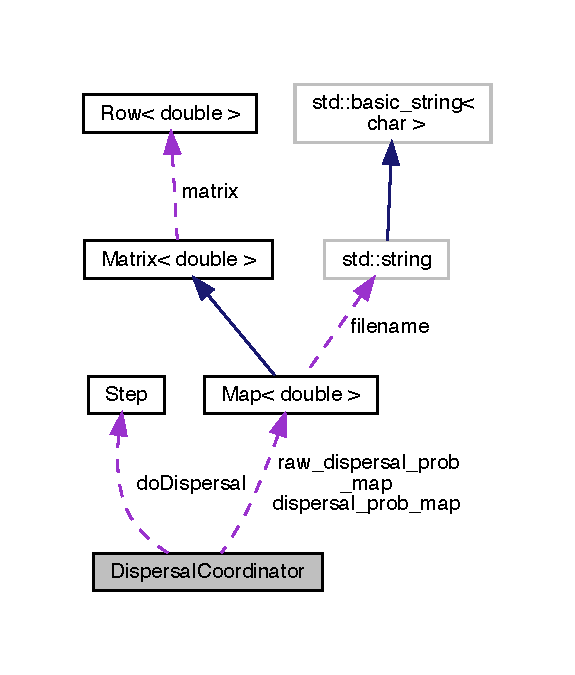
\includegraphics[width=350pt]{class_dispersal_coordinator__coll__graph}
\end{center}
\end{figure}
\subsection*{Public Member Functions}
\begin{DoxyCompactItemize}
\item 
void \hyperlink{class_dispersal_coordinator_a3cfdb18edbf4dd1c45d0cf6af47f91fe}{set\+Random\+Number} (\hyperlink{class_n_rrand}{N\+Rrand} $\ast$N\+R\+\_\+ptr)
\begin{DoxyCompactList}\small\item\em Sets the random number pointer to an \hyperlink{class_n_rrand}{N\+Rrand} instance. \end{DoxyCompactList}\item 
void \hyperlink{class_dispersal_coordinator_a03bc78c6b218366d6165ca49b7e9b35c}{set\+Habitat\+Map} (\hyperlink{class_map}{Map} $\ast$map\+\_\+ptr)
\begin{DoxyCompactList}\small\item\em Sets the pointer to the \hyperlink{class_map}{Map} object. \end{DoxyCompactList}\item 
void \hyperlink{class_dispersal_coordinator_aad9a57afe4629674c958e4d0de4d2451}{set\+Generation\+Ptr} (double $\ast$generation\+\_\+ptr)
\begin{DoxyCompactList}\small\item\em Sets the generation pointer to the provided double. \end{DoxyCompactList}\item 
void \hyperlink{class_dispersal_coordinator_ab0face98d80793e7f4a8ad1bf4dfe3f1}{set\+Dispersal} (const string \&dispersal\+\_\+method, const string \&dispersal\+\_\+file, const unsigned long dispersal\+\_\+x, const unsigned long dispersal\+\_\+y, const double \&m\+\_\+probin, const double \&cutoffin, const double \&sigmain, const double \&tauin, const bool \&restrict\+\_\+self)
\begin{DoxyCompactList}\small\item\em Sets the dispersal method and parameters. \end{DoxyCompactList}\item 
void \hyperlink{class_dispersal_coordinator_a4bac3aeedb3ceb40601c3db951032d0e}{disperse\+Null\+Dispersal\+Map} (\hyperlink{struct_step}{Step} \&this\+\_\+step)
\begin{DoxyCompactList}\small\item\em Picks a random cell from the whole map and stores the value in the step object. \end{DoxyCompactList}\item 
void \hyperlink{class_dispersal_coordinator_a6605069356e02d1c130b6d68e5d08483}{disperse\+Dispersal\+Map} (\hyperlink{struct_step}{Step} \&this\+\_\+step)
\begin{DoxyCompactList}\small\item\em Picks a random dispersal distance from the dispersal map. \end{DoxyCompactList}\item 
void \hyperlink{class_dispersal_coordinator_af2a3792c5e0bea86fa044c4cd3e5146c}{calculate\+Cell\+Coordinates} (\hyperlink{struct_step}{Step} \&this\+\_\+step, const unsigned long \&col\+\_\+ref)
\begin{DoxyCompactList}\small\item\em Calculates the new coordinates for a column reference. This includes converting between the fine map and sample map. New coordinates are saved in this\+\_\+step. \end{DoxyCompactList}\item 
unsigned long \hyperlink{class_dispersal_coordinator_a737c7f1a06650b467d06a91c0474fb79}{calculate\+Cell\+Reference} (\hyperlink{struct_step}{Step} \&this\+\_\+step)
\begin{DoxyCompactList}\small\item\em Calculates the cell reference for a particular coordinate. \end{DoxyCompactList}\item 
void \hyperlink{class_dispersal_coordinator_a79b6018cda012a59f7b80de40b394a6a}{disperse\+Density\+Map} (\hyperlink{struct_step}{Step} \&this\+\_\+step)
\begin{DoxyCompactList}\small\item\em Calls the dispersal kernel from the supplied dispersal distribution. \end{DoxyCompactList}\item 
void \hyperlink{class_dispersal_coordinator_ae72980ec66825c641545675037885248}{set\+End\+Point\+Fptr} (const bool \&restrict\+\_\+self)
\begin{DoxyCompactList}\small\item\em Sets the end point function pointer correctly, based on whether it is restricted or not. \end{DoxyCompactList}\item 
bool \hyperlink{class_dispersal_coordinator_a46fe28ad569bda217e168b33216a888b}{check\+End\+Point} (const unsigned long \&density, long \&oldx, long \&oldy, long \&oldxwrap, long \&oldywrap, const long \&startx, const long \&starty, const long \&startxwrap, const long \&startywrap)
\begin{DoxyCompactList}\small\item\em Check the end point for the given coordinates and density. \end{DoxyCompactList}\item 
bool \hyperlink{class_dispersal_coordinator_a72d8a718590c6dde6f0e8d1ac991d99d}{check\+End\+Point\+Density} (const unsigned long \&density, long \&oldx, long \&oldy, long \&oldxwrap, long \&oldywrap, const long \&startx, const long \&starty, const long \&startxwrap, const long \&startywrap)
\begin{DoxyCompactList}\small\item\em Check the end point for the given coordinates and density. \end{DoxyCompactList}\item 
bool \hyperlink{class_dispersal_coordinator_a055c62c70087ab163bede5c4c4a8be33}{check\+End\+Point\+Restricted} (const unsigned long \&density, long \&oldx, long \&oldy, long \&oldxwrap, long \&oldywrap, const long \&startx, const long \&starty, const long \&startxwrap, const long \&startywrap)
\begin{DoxyCompactList}\small\item\em Check the end point for the given coordinates and density. \end{DoxyCompactList}\item 
void \hyperlink{class_dispersal_coordinator_a08e7c2e1882bd2f83ffd33eed2491fa0}{disperse} (\hyperlink{struct_step}{Step} \&this\+\_\+step)
\begin{DoxyCompactList}\small\item\em Performs the dispersal routine using the \hyperlink{struct_step}{Step} object to read starting positions and record the end positions. \end{DoxyCompactList}\end{DoxyCompactItemize}
\subsection*{Protected Types}
\begin{DoxyCompactItemize}
\item 
typedef void(Dispersal\+Coordinator\+::$\ast$ {\bfseries dispersal\+\_\+fptr}) (\hyperlink{struct_step}{Step} \&this\+\_\+step)\hypertarget{class_dispersal_coordinator_a95a865c016904f23990926af1e7534da}{}\label{class_dispersal_coordinator_a95a865c016904f23990926af1e7534da}

\item 
typedef bool(Dispersal\+Coordinator\+::$\ast$ {\bfseries end\+\_\+fptr}) (const unsigned long \&density, long \&oldx, long \&oldy, long \&oldxwrap, long \&oldywrap, const long \&startx, const long \&starty, const long \&startxwrap, const long \&startywrap)\hypertarget{class_dispersal_coordinator_a6f3d41e77253cb394c63253431decd36}{}\label{class_dispersal_coordinator_a6f3d41e77253cb394c63253431decd36}

\end{DoxyCompactItemize}
\subsection*{Protected Attributes}
\begin{DoxyCompactItemize}
\item 
\hyperlink{class_matrix}{Matrix}$<$ double $>$ {\bfseries dispersal\+\_\+prob\+\_\+map}\hypertarget{class_dispersal_coordinator_a3d780624030ef3d6b3e2b5ae642854fe}{}\label{class_dispersal_coordinator_a3d780624030ef3d6b3e2b5ae642854fe}

\item 
\hyperlink{class_n_rrand}{N\+Rrand} $\ast$ {\bfseries NR}\hypertarget{class_dispersal_coordinator_ac4c17447257ed00e1b5610e0e35a5443}{}\label{class_dispersal_coordinator_ac4c17447257ed00e1b5610e0e35a5443}

\item 
\hyperlink{class_map}{Map} $\ast$ {\bfseries habitat\+\_\+map}\hypertarget{class_dispersal_coordinator_abcd97d006f49882c6f5c4c24df6cb52a}{}\label{class_dispersal_coordinator_abcd97d006f49882c6f5c4c24df6cb52a}

\item 
double $\ast$ {\bfseries generation}\hypertarget{class_dispersal_coordinator_ae3f83d100dad7c60137edf42b3c199c1}{}\label{class_dispersal_coordinator_ae3f83d100dad7c60137edf42b3c199c1}

\item 
dispersal\+\_\+fptr {\bfseries do\+Dispersal}\hypertarget{class_dispersal_coordinator_a93262d2bb612108bfcdc56c1ba11bad1}{}\label{class_dispersal_coordinator_a93262d2bb612108bfcdc56c1ba11bad1}

\item 
end\+\_\+fptr {\bfseries check\+End\+Point\+Fptr}\hypertarget{class_dispersal_coordinator_a1612005c176cd769797a4d4e459e2dec}{}\label{class_dispersal_coordinator_a1612005c176cd769797a4d4e459e2dec}

\item 
unsigned long {\bfseries xdim}\hypertarget{class_dispersal_coordinator_a66668e6ceec55afa61c1e99719bc6146}{}\label{class_dispersal_coordinator_a66668e6ceec55afa61c1e99719bc6146}

\end{DoxyCompactItemize}


\subsection{Detailed Description}
Class for generating dispersal distances and provide routines for reading dispersal distance maps as a unwound map-\/of-\/maps. This class also handles reading density maps for rejection sampling. 

It requires linking to a density map, random number generator and a generation counter from the \hyperlink{class_tree}{Tree} class.

Note that no element of this object is recorded during a paused simulation, as all objects pointed to are stored elsewhere and behaviours are recalculated upon simulation resume. 

\subsection{Member Function Documentation}
\index{Dispersal\+Coordinator@{Dispersal\+Coordinator}!calculate\+Cell\+Coordinates@{calculate\+Cell\+Coordinates}}
\index{calculate\+Cell\+Coordinates@{calculate\+Cell\+Coordinates}!Dispersal\+Coordinator@{Dispersal\+Coordinator}}
\subsubsection[{\texorpdfstring{calculate\+Cell\+Coordinates(\+Step \&this\+\_\+step, const unsigned long \&col\+\_\+ref)}{calculateCellCoordinates(Step &this_step, const unsigned long &col_ref)}}]{\setlength{\rightskip}{0pt plus 5cm}void Dispersal\+Coordinator\+::calculate\+Cell\+Coordinates (
\begin{DoxyParamCaption}
\item[{{\bf Step} \&}]{this\+\_\+step, }
\item[{const unsigned long \&}]{col\+\_\+ref}
\end{DoxyParamCaption}
)}\hypertarget{class_dispersal_coordinator_af2a3792c5e0bea86fa044c4cd3e5146c}{}\label{class_dispersal_coordinator_af2a3792c5e0bea86fa044c4cd3e5146c}


Calculates the new coordinates for a column reference. This includes converting between the fine map and sample map. New coordinates are saved in this\+\_\+step. 


\begin{DoxyParams}{Parameters}
{\em this\+\_\+step} & the step to save new coordinates in. \\
\hline
{\em col\+\_\+ref} & the column reference for \\
\hline
\end{DoxyParams}
\index{Dispersal\+Coordinator@{Dispersal\+Coordinator}!calculate\+Cell\+Reference@{calculate\+Cell\+Reference}}
\index{calculate\+Cell\+Reference@{calculate\+Cell\+Reference}!Dispersal\+Coordinator@{Dispersal\+Coordinator}}
\subsubsection[{\texorpdfstring{calculate\+Cell\+Reference(\+Step \&this\+\_\+step)}{calculateCellReference(Step &this_step)}}]{\setlength{\rightskip}{0pt plus 5cm}unsigned long Dispersal\+Coordinator\+::calculate\+Cell\+Reference (
\begin{DoxyParamCaption}
\item[{{\bf Step} \&}]{this\+\_\+step}
\end{DoxyParamCaption}
)}\hypertarget{class_dispersal_coordinator_a737c7f1a06650b467d06a91c0474fb79}{}\label{class_dispersal_coordinator_a737c7f1a06650b467d06a91c0474fb79}


Calculates the cell reference for a particular coordinate. 

The formula for this calculation is x + (y $\ast$ xdim) where xdim is the dimensions of the fine map, and x and y are the coordinates for the fine map


\begin{DoxyParams}{Parameters}
{\em this\+\_\+step} & the step object containing the x, y location, and x,y wrapping \\
\hline
\end{DoxyParams}
\begin{DoxyReturn}{Returns}
the cell reference from the dispersal\+\_\+prob\+\_\+map which corresponds to the required cell 
\end{DoxyReturn}
\index{Dispersal\+Coordinator@{Dispersal\+Coordinator}!check\+End\+Point@{check\+End\+Point}}
\index{check\+End\+Point@{check\+End\+Point}!Dispersal\+Coordinator@{Dispersal\+Coordinator}}
\subsubsection[{\texorpdfstring{check\+End\+Point(const unsigned long \&density, long \&oldx, long \&oldy, long \&oldxwrap, long \&oldywrap, const long \&startx, const long \&starty, const long \&startxwrap, const long \&startywrap)}{checkEndPoint(const unsigned long &density, long &oldx, long &oldy, long &oldxwrap, long &oldywrap, const long &startx, const long &starty, const long &startxwrap, const long &startywrap)}}]{\setlength{\rightskip}{0pt plus 5cm}bool Dispersal\+Coordinator\+::check\+End\+Point (
\begin{DoxyParamCaption}
\item[{const unsigned long \&}]{density, }
\item[{long \&}]{oldx, }
\item[{long \&}]{oldy, }
\item[{long \&}]{oldxwrap, }
\item[{long \&}]{oldywrap, }
\item[{const long \&}]{startx, }
\item[{const long \&}]{starty, }
\item[{const long \&}]{startxwrap, }
\item[{const long \&}]{startywrap}
\end{DoxyParamCaption}
)}\hypertarget{class_dispersal_coordinator_a46fe28ad569bda217e168b33216a888b}{}\label{class_dispersal_coordinator_a46fe28ad569bda217e168b33216a888b}


Check the end point for the given coordinates and density. 


\begin{DoxyParams}{Parameters}
{\em density} & the density at the end point -\/ avoids an extra call to \hyperlink{class_map_ab96b3097832c620a024184ed54d5e2d1}{Map\+::get\+Val()} \\
\hline
{\em oldx} & the old x position \\
\hline
{\em oldy} & the old y position \\
\hline
{\em oldxwrap} & the old x wrap \\
\hline
{\em oldywrap} & the old y wrap \\
\hline
{\em startx} & the starting x position \\
\hline
{\em starty} & the starting y position \\
\hline
{\em startxwrap} & the starting x wrap \\
\hline
{\em startywrap} & the ending y wrap \\
\hline
\end{DoxyParams}
\begin{DoxyReturn}{Returns}
true if the end point passes the density and restricted checks 
\end{DoxyReturn}
\index{Dispersal\+Coordinator@{Dispersal\+Coordinator}!check\+End\+Point\+Density@{check\+End\+Point\+Density}}
\index{check\+End\+Point\+Density@{check\+End\+Point\+Density}!Dispersal\+Coordinator@{Dispersal\+Coordinator}}
\subsubsection[{\texorpdfstring{check\+End\+Point\+Density(const unsigned long \&density, long \&oldx, long \&oldy, long \&oldxwrap, long \&oldywrap, const long \&startx, const long \&starty, const long \&startxwrap, const long \&startywrap)}{checkEndPointDensity(const unsigned long &density, long &oldx, long &oldy, long &oldxwrap, long &oldywrap, const long &startx, const long &starty, const long &startxwrap, const long &startywrap)}}]{\setlength{\rightskip}{0pt plus 5cm}bool Dispersal\+Coordinator\+::check\+End\+Point\+Density (
\begin{DoxyParamCaption}
\item[{const unsigned long \&}]{density, }
\item[{long \&}]{oldx, }
\item[{long \&}]{oldy, }
\item[{long \&}]{oldxwrap, }
\item[{long \&}]{oldywrap, }
\item[{const long \&}]{startx, }
\item[{const long \&}]{starty, }
\item[{const long \&}]{startxwrap, }
\item[{const long \&}]{startywrap}
\end{DoxyParamCaption}
)}\hypertarget{class_dispersal_coordinator_a72d8a718590c6dde6f0e8d1ac991d99d}{}\label{class_dispersal_coordinator_a72d8a718590c6dde6f0e8d1ac991d99d}


Check the end point for the given coordinates and density. 


\begin{DoxyParams}{Parameters}
{\em density} & the density at the end point -\/ avoids an extra call to \hyperlink{class_map_ab96b3097832c620a024184ed54d5e2d1}{Map\+::get\+Val()} \\
\hline
{\em oldx} & the old x position \\
\hline
{\em oldy} & the old y position \\
\hline
{\em oldxwrap} & the old x wrap \\
\hline
{\em oldywrap} & the old y wrap \\
\hline
{\em startx} & the starting x position \\
\hline
{\em starty} & the starting y position \\
\hline
{\em startxwrap} & the starting x wrap \\
\hline
{\em startywrap} & the ending y wrap \\
\hline
\end{DoxyParams}
\begin{DoxyReturn}{Returns}
true if the end point passes the density and restricted checks 
\end{DoxyReturn}
\index{Dispersal\+Coordinator@{Dispersal\+Coordinator}!check\+End\+Point\+Restricted@{check\+End\+Point\+Restricted}}
\index{check\+End\+Point\+Restricted@{check\+End\+Point\+Restricted}!Dispersal\+Coordinator@{Dispersal\+Coordinator}}
\subsubsection[{\texorpdfstring{check\+End\+Point\+Restricted(const unsigned long \&density, long \&oldx, long \&oldy, long \&oldxwrap, long \&oldywrap, const long \&startx, const long \&starty, const long \&startxwrap, const long \&startywrap)}{checkEndPointRestricted(const unsigned long &density, long &oldx, long &oldy, long &oldxwrap, long &oldywrap, const long &startx, const long &starty, const long &startxwrap, const long &startywrap)}}]{\setlength{\rightskip}{0pt plus 5cm}bool Dispersal\+Coordinator\+::check\+End\+Point\+Restricted (
\begin{DoxyParamCaption}
\item[{const unsigned long \&}]{density, }
\item[{long \&}]{oldx, }
\item[{long \&}]{oldy, }
\item[{long \&}]{oldxwrap, }
\item[{long \&}]{oldywrap, }
\item[{const long \&}]{startx, }
\item[{const long \&}]{starty, }
\item[{const long \&}]{startxwrap, }
\item[{const long \&}]{startywrap}
\end{DoxyParamCaption}
)}\hypertarget{class_dispersal_coordinator_a055c62c70087ab163bede5c4c4a8be33}{}\label{class_dispersal_coordinator_a055c62c70087ab163bede5c4c4a8be33}


Check the end point for the given coordinates and density. 


\begin{DoxyParams}{Parameters}
{\em density} & the density at the end point -\/ avoids an extra call to \hyperlink{class_map_ab96b3097832c620a024184ed54d5e2d1}{Map\+::get\+Val()} \\
\hline
{\em oldx} & the old x position \\
\hline
{\em oldy} & the old y position \\
\hline
{\em oldxwrap} & the old x wrap \\
\hline
{\em oldywrap} & the old y wrap \\
\hline
{\em startx} & the starting x position \\
\hline
{\em starty} & the starting y position \\
\hline
{\em startxwrap} & the starting x wrap \\
\hline
{\em startywrap} & the ending y wrap \\
\hline
\end{DoxyParams}
\begin{DoxyReturn}{Returns}
true if the end point passes the density and restricted checks 
\end{DoxyReturn}
\index{Dispersal\+Coordinator@{Dispersal\+Coordinator}!disperse@{disperse}}
\index{disperse@{disperse}!Dispersal\+Coordinator@{Dispersal\+Coordinator}}
\subsubsection[{\texorpdfstring{disperse(\+Step \&this\+\_\+step)}{disperse(Step &this_step)}}]{\setlength{\rightskip}{0pt plus 5cm}void Dispersal\+Coordinator\+::disperse (
\begin{DoxyParamCaption}
\item[{{\bf Step} \&}]{this\+\_\+step}
\end{DoxyParamCaption}
)}\hypertarget{class_dispersal_coordinator_a08e7c2e1882bd2f83ffd33eed2491fa0}{}\label{class_dispersal_coordinator_a08e7c2e1882bd2f83ffd33eed2491fa0}


Performs the dispersal routine using the \hyperlink{struct_step}{Step} object to read starting positions and record the end positions. 


\begin{DoxyParams}{Parameters}
{\em this\+\_\+step} & the \hyperlink{struct_step}{Step} object for reading starting position and storing output distances and angles \\
\hline
\end{DoxyParams}
\index{Dispersal\+Coordinator@{Dispersal\+Coordinator}!disperse\+Density\+Map@{disperse\+Density\+Map}}
\index{disperse\+Density\+Map@{disperse\+Density\+Map}!Dispersal\+Coordinator@{Dispersal\+Coordinator}}
\subsubsection[{\texorpdfstring{disperse\+Density\+Map(\+Step \&this\+\_\+step)}{disperseDensityMap(Step &this_step)}}]{\setlength{\rightskip}{0pt plus 5cm}void Dispersal\+Coordinator\+::disperse\+Density\+Map (
\begin{DoxyParamCaption}
\item[{{\bf Step} \&}]{this\+\_\+step}
\end{DoxyParamCaption}
)}\hypertarget{class_dispersal_coordinator_a79b6018cda012a59f7b80de40b394a6a}{}\label{class_dispersal_coordinator_a79b6018cda012a59f7b80de40b394a6a}


Calls the dispersal kernel from the supplied dispersal distribution. 


\begin{DoxyParams}{Parameters}
{\em this\+\_\+step} & the step object to store end points in \\
\hline
\end{DoxyParams}
\index{Dispersal\+Coordinator@{Dispersal\+Coordinator}!disperse\+Dispersal\+Map@{disperse\+Dispersal\+Map}}
\index{disperse\+Dispersal\+Map@{disperse\+Dispersal\+Map}!Dispersal\+Coordinator@{Dispersal\+Coordinator}}
\subsubsection[{\texorpdfstring{disperse\+Dispersal\+Map(\+Step \&this\+\_\+step)}{disperseDispersalMap(Step &this_step)}}]{\setlength{\rightskip}{0pt plus 5cm}void Dispersal\+Coordinator\+::disperse\+Dispersal\+Map (
\begin{DoxyParamCaption}
\item[{{\bf Step} \&}]{this\+\_\+step}
\end{DoxyParamCaption}
)}\hypertarget{class_dispersal_coordinator_a6605069356e02d1c130b6d68e5d08483}{}\label{class_dispersal_coordinator_a6605069356e02d1c130b6d68e5d08483}


Picks a random dispersal distance from the dispersal map. 


\begin{DoxyParams}{Parameters}
{\em this\+\_\+step} & the step object to store end points in \\
\hline
\end{DoxyParams}
\index{Dispersal\+Coordinator@{Dispersal\+Coordinator}!disperse\+Null\+Dispersal\+Map@{disperse\+Null\+Dispersal\+Map}}
\index{disperse\+Null\+Dispersal\+Map@{disperse\+Null\+Dispersal\+Map}!Dispersal\+Coordinator@{Dispersal\+Coordinator}}
\subsubsection[{\texorpdfstring{disperse\+Null\+Dispersal\+Map(\+Step \&this\+\_\+step)}{disperseNullDispersalMap(Step &this_step)}}]{\setlength{\rightskip}{0pt plus 5cm}void Dispersal\+Coordinator\+::disperse\+Null\+Dispersal\+Map (
\begin{DoxyParamCaption}
\item[{{\bf Step} \&}]{this\+\_\+step}
\end{DoxyParamCaption}
)}\hypertarget{class_dispersal_coordinator_a4bac3aeedb3ceb40601c3db951032d0e}{}\label{class_dispersal_coordinator_a4bac3aeedb3ceb40601c3db951032d0e}


Picks a random cell from the whole map and stores the value in the step object. 


\begin{DoxyParams}{Parameters}
{\em this\+\_\+step} & the step object to store end points in \\
\hline
\end{DoxyParams}
\index{Dispersal\+Coordinator@{Dispersal\+Coordinator}!set\+Dispersal@{set\+Dispersal}}
\index{set\+Dispersal@{set\+Dispersal}!Dispersal\+Coordinator@{Dispersal\+Coordinator}}
\subsubsection[{\texorpdfstring{set\+Dispersal(const string \&dispersal\+\_\+method, const string \&dispersal\+\_\+file, const unsigned long dispersal\+\_\+x, const unsigned long dispersal\+\_\+y, const double \&m\+\_\+probin, const double \&cutoffin, const double \&sigmain, const double \&tauin, const bool \&restrict\+\_\+self)}{setDispersal(const string &dispersal_method, const string &dispersal_file, const unsigned long dispersal_x, const unsigned long dispersal_y, const double &m_probin, const double &cutoffin, const double &sigmain, const double &tauin, const bool &restrict_self)}}]{\setlength{\rightskip}{0pt plus 5cm}void Dispersal\+Coordinator\+::set\+Dispersal (
\begin{DoxyParamCaption}
\item[{const string \&}]{dispersal\+\_\+method, }
\item[{const string \&}]{dispersal\+\_\+file, }
\item[{const unsigned long}]{dispersal\+\_\+x, }
\item[{const unsigned long}]{dispersal\+\_\+y, }
\item[{const double \&}]{m\+\_\+probin, }
\item[{const double \&}]{cutoffin, }
\item[{const double \&}]{sigmain, }
\item[{const double \&}]{tauin, }
\item[{const bool \&}]{restrict\+\_\+self}
\end{DoxyParamCaption}
)}\hypertarget{class_dispersal_coordinator_ab0face98d80793e7f4a8ad1bf4dfe3f1}{}\label{class_dispersal_coordinator_ab0face98d80793e7f4a8ad1bf4dfe3f1}


Sets the dispersal method and parameters. 


\begin{DoxyParams}{Parameters}
{\em dispersal\+\_\+method} & string containing the dispersal type. Can be one of \mbox{[}normal, fat-\/tail, norm-\/uniform\mbox{]} \\
\hline
{\em dispersal\+\_\+file} & string containing the dispersal file, or \char`\"{}none\char`\"{} if using dispersal kernel \\
\hline
{\em m\+\_\+probin} & the probability of drawing from the uniform distribution. Only relevant for uniform dispersals \\
\hline
{\em cutoffin} & the maximum value to be drawn from the uniform dispersal. Only relevant for uniform dispersals \\
\hline
{\em sigmain} & the fatness of the fat-\/tailed dispersal kernel \\
\hline
{\em tauin} & the width of the fat-\/tailed dispersal kernel \\
\hline
{\em restrict\+\_\+self} & if true, denies possibility that dispersal comes from the same cell as the parent \\
\hline
\end{DoxyParams}
\index{Dispersal\+Coordinator@{Dispersal\+Coordinator}!set\+End\+Point\+Fptr@{set\+End\+Point\+Fptr}}
\index{set\+End\+Point\+Fptr@{set\+End\+Point\+Fptr}!Dispersal\+Coordinator@{Dispersal\+Coordinator}}
\subsubsection[{\texorpdfstring{set\+End\+Point\+Fptr(const bool \&restrict\+\_\+self)}{setEndPointFptr(const bool &restrict_self)}}]{\setlength{\rightskip}{0pt plus 5cm}void Dispersal\+Coordinator\+::set\+End\+Point\+Fptr (
\begin{DoxyParamCaption}
\item[{const bool \&}]{restrict\+\_\+self}
\end{DoxyParamCaption}
)}\hypertarget{class_dispersal_coordinator_ae72980ec66825c641545675037885248}{}\label{class_dispersal_coordinator_ae72980ec66825c641545675037885248}


Sets the end point function pointer correctly, based on whether it is restricted or not. 


\begin{DoxyParams}{Parameters}
{\em restrict\+\_\+self} & if true, denies possibility that dispersal comes from the same cell as the parent \\
\hline
\end{DoxyParams}
\index{Dispersal\+Coordinator@{Dispersal\+Coordinator}!set\+Generation\+Ptr@{set\+Generation\+Ptr}}
\index{set\+Generation\+Ptr@{set\+Generation\+Ptr}!Dispersal\+Coordinator@{Dispersal\+Coordinator}}
\subsubsection[{\texorpdfstring{set\+Generation\+Ptr(double $\ast$generation\+\_\+ptr)}{setGenerationPtr(double *generation_ptr)}}]{\setlength{\rightskip}{0pt plus 5cm}void Dispersal\+Coordinator\+::set\+Generation\+Ptr (
\begin{DoxyParamCaption}
\item[{double $\ast$}]{generation\+\_\+ptr}
\end{DoxyParamCaption}
)}\hypertarget{class_dispersal_coordinator_aad9a57afe4629674c958e4d0de4d2451}{}\label{class_dispersal_coordinator_aad9a57afe4629674c958e4d0de4d2451}


Sets the generation pointer to the provided double. 


\begin{DoxyParams}{Parameters}
{\em generation\+\_\+ptr} & pointer to the generation double \\
\hline
\end{DoxyParams}
\index{Dispersal\+Coordinator@{Dispersal\+Coordinator}!set\+Habitat\+Map@{set\+Habitat\+Map}}
\index{set\+Habitat\+Map@{set\+Habitat\+Map}!Dispersal\+Coordinator@{Dispersal\+Coordinator}}
\subsubsection[{\texorpdfstring{set\+Habitat\+Map(\+Map $\ast$map\+\_\+ptr)}{setHabitatMap(Map *map_ptr)}}]{\setlength{\rightskip}{0pt plus 5cm}void Dispersal\+Coordinator\+::set\+Habitat\+Map (
\begin{DoxyParamCaption}
\item[{{\bf Map} $\ast$}]{map\+\_\+ptr}
\end{DoxyParamCaption}
)}\hypertarget{class_dispersal_coordinator_a03bc78c6b218366d6165ca49b7e9b35c}{}\label{class_dispersal_coordinator_a03bc78c6b218366d6165ca49b7e9b35c}


Sets the pointer to the \hyperlink{class_map}{Map} object. 


\begin{DoxyParams}{Parameters}
{\em map\+\_\+ptr} & pointer to a \hyperlink{class_map}{Map} object \\
\hline
\end{DoxyParams}
\index{Dispersal\+Coordinator@{Dispersal\+Coordinator}!set\+Random\+Number@{set\+Random\+Number}}
\index{set\+Random\+Number@{set\+Random\+Number}!Dispersal\+Coordinator@{Dispersal\+Coordinator}}
\subsubsection[{\texorpdfstring{set\+Random\+Number(\+N\+Rrand $\ast$\+N\+R\+\_\+ptr)}{setRandomNumber(NRrand *NR_ptr)}}]{\setlength{\rightskip}{0pt plus 5cm}void Dispersal\+Coordinator\+::set\+Random\+Number (
\begin{DoxyParamCaption}
\item[{{\bf N\+Rrand} $\ast$}]{N\+R\+\_\+ptr}
\end{DoxyParamCaption}
)}\hypertarget{class_dispersal_coordinator_a3cfdb18edbf4dd1c45d0cf6af47f91fe}{}\label{class_dispersal_coordinator_a3cfdb18edbf4dd1c45d0cf6af47f91fe}


Sets the random number pointer to an \hyperlink{class_n_rrand}{N\+Rrand} instance. 


\begin{DoxyParams}{Parameters}
{\em N\+R\+\_\+ptr} & the random number object to set to \\
\hline
\end{DoxyParams}


The documentation for this class was generated from the following files\+:\begin{DoxyCompactItemize}
\item 
necsim/\hyperlink{_dispersal_coordinator_8h}{Dispersal\+Coordinator.\+h}\item 
necsim/\hyperlink{_dispersal_coordinator_8cpp}{Dispersal\+Coordinator.\+cpp}\end{DoxyCompactItemize}

\hypertarget{struct_fatal___exception}{}\section{Fatal\+\_\+\+Exception Struct Reference}
\label{struct_fatal___exception}\index{Fatal\+\_\+\+Exception@{Fatal\+\_\+\+Exception}}


This is called any time a fatal exception is called and the program is unwound and ended.  




{\ttfamily \#include $<$Custom\+Exceptions.\+h$>$}



Inheritance diagram for Fatal\+\_\+\+Exception\+:
% FIG 0


Collaboration diagram for Fatal\+\_\+\+Exception\+:
% FIG 1
\subsection*{Public Member Functions}
\begin{DoxyCompactItemize}
\item 
{\bfseries Fatal\+\_\+\+Exception} (string msg)\hypertarget{struct_fatal___exception_ab288be87b35a7efa13bd7f1eca94f28a}{}\label{struct_fatal___exception_ab288be87b35a7efa13bd7f1eca94f28a}

\end{DoxyCompactItemize}


\subsection{Detailed Description}
This is called any time a fatal exception is called and the program is unwound and ended. 

The documentation for this struct was generated from the following file\+:\begin{DoxyCompactItemize}
\item 
\hyperlink{_custom_exceptions_8h}{Custom\+Exceptions.\+h}\end{DoxyCompactItemize}

\hypertarget{struct_fragment}{}\section{Fragment Struct Reference}
\label{struct_fragment}\index{Fragment@{Fragment}}


Contains the information needed for defining a fragment. Fragments can be detected from the \hyperlink{class_samplematrix}{Samplematrix} object (which only detects rectangular fragments), or (preferably) is read from an input file. Currently all fragments must be rectangular, although they can be larger than the intended shape if necesssary.  




{\ttfamily \#include $<$Community.\+h$>$}



Collaboration diagram for Fragment\+:
\nopagebreak
\begin{figure}[H]
\begin{center}
\leavevmode
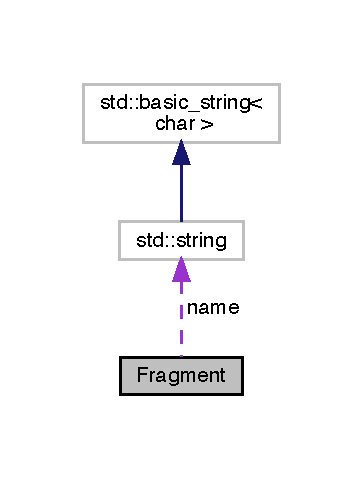
\includegraphics[width=174pt]{struct_fragment__coll__graph}
\end{center}
\end{figure}
\subsection*{Public Attributes}
\begin{DoxyCompactItemize}
\item 
string {\bfseries name}\hypertarget{struct_fragment_acf92da0ecedecb7080adf56e35543636}{}\label{struct_fragment_acf92da0ecedecb7080adf56e35543636}

\item 
long {\bfseries x\+\_\+east}\hypertarget{struct_fragment_a0257d6b1942656e4181eab82cc5392c4}{}\label{struct_fragment_a0257d6b1942656e4181eab82cc5392c4}

\item 
long {\bfseries x\+\_\+west}\hypertarget{struct_fragment_aabfd09652d5abae4b6393fd40e6d3d9d}{}\label{struct_fragment_aabfd09652d5abae4b6393fd40e6d3d9d}

\item 
long {\bfseries y\+\_\+north}\hypertarget{struct_fragment_a1d792c8e975cbc9405ece3a90a283c4f}{}\label{struct_fragment_a1d792c8e975cbc9405ece3a90a283c4f}

\item 
long {\bfseries y\+\_\+south}\hypertarget{struct_fragment_a71d7c613d71459b72158ef80ba705bfc}{}\label{struct_fragment_a71d7c613d71459b72158ef80ba705bfc}

\item 
unsigned long {\bfseries num}\hypertarget{struct_fragment_ac966a3ac928cba2706ca9c87f159d1ee}{}\label{struct_fragment_ac966a3ac928cba2706ca9c87f159d1ee}

\item 
double {\bfseries area}\hypertarget{struct_fragment_ad37e6d449d9b0b1273e712e5a4da2887}{}\label{struct_fragment_ad37e6d449d9b0b1273e712e5a4da2887}

\end{DoxyCompactItemize}


\subsection{Detailed Description}
Contains the information needed for defining a fragment. Fragments can be detected from the \hyperlink{class_samplematrix}{Samplematrix} object (which only detects rectangular fragments), or (preferably) is read from an input file. Currently all fragments must be rectangular, although they can be larger than the intended shape if necesssary. 

The documentation for this struct was generated from the following file\+:\begin{DoxyCompactItemize}
\item 
necsim/Community.\+h\end{DoxyCompactItemize}

\hypertarget{struct_main___exception}{}\section{Main\+\_\+\+Exception Struct Reference}
\label{struct_main___exception}\index{Main\+\_\+\+Exception@{Main\+\_\+\+Exception}}


These are used for non-\/fatal exception thrown from within the main simulation where no-\/more specific location information is possible.  




{\ttfamily \#include $<$Custom\+Exceptions.\+h$>$}



Inheritance diagram for Main\+\_\+\+Exception\+:
% FIG 0


Collaboration diagram for Main\+\_\+\+Exception\+:
% FIG 1
\subsection*{Public Member Functions}
\begin{DoxyCompactItemize}
\item 
{\bfseries Main\+\_\+\+Exception} (string msg)\hypertarget{struct_main___exception_a3b56c19b4513c6695cea80d90ca7da8f}{}\label{struct_main___exception_a3b56c19b4513c6695cea80d90ca7da8f}

\end{DoxyCompactItemize}


\subsection{Detailed Description}
These are used for non-\/fatal exception thrown from within the main simulation where no-\/more specific location information is possible. 

The documentation for this struct was generated from the following file\+:\begin{DoxyCompactItemize}
\item 
\hyperlink{_custom_exceptions_8h}{Custom\+Exceptions.\+h}\end{DoxyCompactItemize}

\hypertarget{class_map}{}\section{Map$<$ T $>$ Class Template Reference}
\label{class_map}\index{Map$<$ T $>$@{Map$<$ T $>$}}


Read a a tif file to a matrix and obtain spatial metadata.  




{\ttfamily \#include $<$Map.\+h$>$}



Inheritance diagram for Map$<$ T $>$\+:
\nopagebreak
\begin{figure}[H]
\begin{center}
\leavevmode
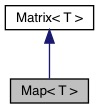
\includegraphics[width=146pt]{class_map__inherit__graph}
\end{center}
\end{figure}


Collaboration diagram for Map$<$ T $>$\+:
\nopagebreak
\begin{figure}[H]
\begin{center}
\leavevmode
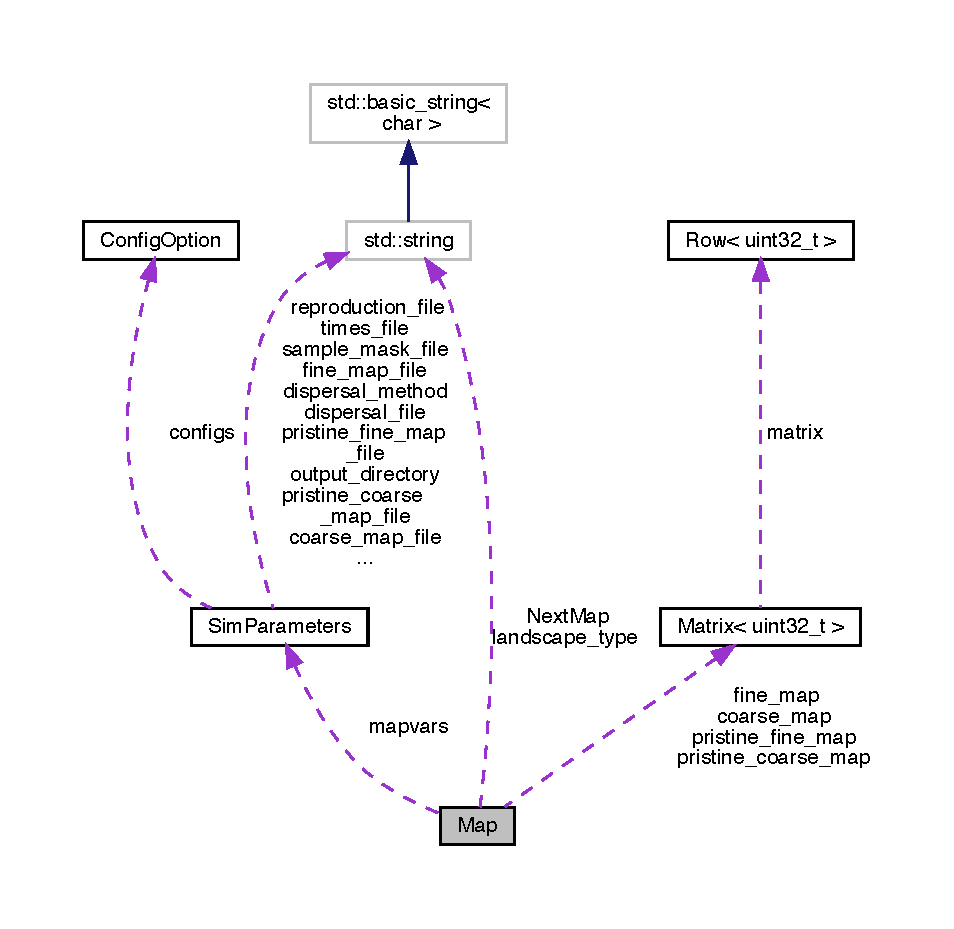
\includegraphics[width=241pt]{class_map__coll__graph}
\end{center}
\end{figure}
\subsection*{Public Member Functions}
\begin{DoxyCompactItemize}
\item 
void \hyperlink{class_map_aa2764c9ae1c54c1821fa4f63b88fe0f3}{open} (const string \&filename\+\_\+in)
\begin{DoxyCompactList}\small\item\em Opens the provided filename to the po\+Dataset object. \end{DoxyCompactList}\item 
void \hyperlink{class_map_a2389e09950706ef49640976837186c79}{open} ()\hypertarget{class_map_a2389e09950706ef49640976837186c79}{}\label{class_map_a2389e09950706ef49640976837186c79}

\begin{DoxyCompactList}\small\item\em Overloaded open for using the preset file name. \end{DoxyCompactList}\item 
bool \hyperlink{class_map_a19f6874b008fcbfac213341d05c2f443}{is\+Open} ()
\begin{DoxyCompactList}\small\item\em Checks if the connection to the map file has already been opened. \end{DoxyCompactList}\item 
void \hyperlink{class_map_ad73fafd17ff95872e9b63945584ae81f}{close} ()\hypertarget{class_map_ad73fafd17ff95872e9b63945584ae81f}{}\label{class_map_ad73fafd17ff95872e9b63945584ae81f}

\begin{DoxyCompactList}\small\item\em Destroys the connection to the dataset. \end{DoxyCompactList}\item 
void \hyperlink{class_map_ade2338d7a8d598c343208b633f8a3a93}{get\+Raster\+Band} ()\hypertarget{class_map_ade2338d7a8d598c343208b633f8a3a93}{}\label{class_map_ade2338d7a8d598c343208b633f8a3a93}

\begin{DoxyCompactList}\small\item\em Sets the raster band to the first raster. \end{DoxyCompactList}\item 
void \hyperlink{class_map_a4e441dcda33d78bef193b1ad1265b5e8}{get\+Block\+Sizes} ()\hypertarget{class_map_a4e441dcda33d78bef193b1ad1265b5e8}{}\label{class_map_a4e441dcda33d78bef193b1ad1265b5e8}

\begin{DoxyCompactList}\small\item\em Obtains the x and y dimensions from the tif file for reading in blocks. \end{DoxyCompactList}\item 
void \hyperlink{class_map_a180284cfba3442eb3d62fc41d0d8f546}{get\+Meta\+Data} ()\hypertarget{class_map_a180284cfba3442eb3d62fc41d0d8f546}{}\label{class_map_a180284cfba3442eb3d62fc41d0d8f546}

\begin{DoxyCompactList}\small\item\em Sets the no data, data type and data type name values from the tif file. \end{DoxyCompactList}\item 
double \hyperlink{class_map_afd32790ea28d0c5aa99b582b2d474933}{get\+Upper\+LeftX} ()
\begin{DoxyCompactList}\small\item\em Gets the upper left x (longitude) coordinate. \end{DoxyCompactList}\item 
double \hyperlink{class_map_a2d7b63836d06b2710192e7c8afd38641}{get\+Upper\+LeftY} ()
\begin{DoxyCompactList}\small\item\em Gets the upper left y (latitude) coordinate. \end{DoxyCompactList}\item 
void \hyperlink{class_map_ad1a25204dce37addc3453e091552b014}{import} (const string \&filename) override
\begin{DoxyCompactList}\small\item\em Imports the matrix from a csv file. \end{DoxyCompactList}\item 
bool \hyperlink{class_map_a2306683b0b3b4ddb7d776d1ff60d4491}{import\+Tif} (const string \&filename)
\begin{DoxyCompactList}\small\item\em Imports the matrix from a tif file using the gdal library functions. \end{DoxyCompactList}\item 
bool \hyperlink{class_map_ade20cc1876ba2774f0f8274d432d89c3}{open\+Offset\+Map} (\hyperlink{class_map}{Map} \&offset\+\_\+map)
\begin{DoxyCompactList}\small\item\em Opens the offset map and fetches the metadata. \end{DoxyCompactList}\item 
void {\bfseries close\+Offset\+Map} (\hyperlink{class_map}{Map} \&offset\+\_\+map, const bool \&opened\+\_\+here)\hypertarget{class_map_a39d76e341e0f817d65ddf0100cfe5f26}{}\label{class_map_a39d76e341e0f817d65ddf0100cfe5f26}

\item 
void \hyperlink{class_map_a200701b23560dd38238801522b234e78}{calculate\+Offset} (\hyperlink{class_map}{Map} \&offset\+\_\+map, long \&offset\+\_\+x, long \&offset\+\_\+y)
\begin{DoxyCompactList}\small\item\em Calculates the offset between the two maps. \end{DoxyCompactList}\item 
unsigned long \hyperlink{class_map_a9862291ea99fe1718d758213b3687bd8}{rounded\+Scale} (\hyperlink{class_map}{Map} \&offset\+\_\+map)
\begin{DoxyCompactList}\small\item\em Calculates the relative scale of this map compared to the offset map. \end{DoxyCompactList}\item 
void \hyperlink{class_map_a0c17360ca7fa935d59f2169fd0007630}{internal\+Import} ()
\begin{DoxyCompactList}\small\item\em Default importer when we rely on the default gdal method of converting between values. Note that importing doubles to ints results in the values being rounded down. \end{DoxyCompactList}\item 
void \hyperlink{class_map_a414e6bc9305ab830836cf817cb4a0d60}{default\+Import} ()\hypertarget{class_map_a414e6bc9305ab830836cf817cb4a0d60}{}\label{class_map_a414e6bc9305ab830836cf817cb4a0d60}

\begin{DoxyCompactList}\small\item\em Default import routine for any type. Provided as a separate function so implementation can be called from any template class type. \end{DoxyCompactList}\item 
void \hyperlink{class_map_aaefe833ab35a68ce54e7eec996c48971}{import\+From\+Double\+And\+Make\+Bool} ()\hypertarget{class_map_aaefe833ab35a68ce54e7eec996c48971}{}\label{class_map_aaefe833ab35a68ce54e7eec996c48971}

\begin{DoxyCompactList}\small\item\em Imports from the supplied filename into the Geo\+Tiff object, converting doubles to booleans. The threshold for conversion is x$>$0.\+5 -\/$>$ true, false otherwise. \end{DoxyCompactList}\item 
{\footnotesize template$<$typename T2 $>$ }\\void \hyperlink{class_map_ae88574927ad3a38fc0a9bc253a9e4a7a}{import\+Using\+Buffer} (G\+D\+A\+L\+Data\+Type dt\+\_\+buff)
\begin{DoxyCompactList}\small\item\em Imports from the supplied filename into the Geo\+Tiff object, converting doubles to booleans. The threshold for conversion is x$>$0.\+5 -\/$>$ true, false otherwise. \end{DoxyCompactList}\item 
void \hyperlink{class_map_a03e0486e704090765d253b18a9dde0f5}{print\+Number\+Complete} (const uint32\+\_\+t \&j, unsigned int \&number\+\_\+printed)
\begin{DoxyCompactList}\small\item\em Print the percentage complete during import. \end{DoxyCompactList}\item 
void \hyperlink{class_map_a6387185da6dc3063cd2311ffab0a5fba}{check\+Tif\+Import\+Failure} ()\hypertarget{class_map_a6387185da6dc3063cd2311ffab0a5fba}{}\label{class_map_a6387185da6dc3063cd2311ffab0a5fba}

\begin{DoxyCompactList}\small\item\em Checks the error code of the C\+P\+L\+Err object and formats the error. \end{DoxyCompactList}\item 
\hyperlink{class_map}{Map} \& \hyperlink{class_map_a00f73ad13cb67e3c4836fae9614d6b40}{operator=} (const \hyperlink{class_map}{Map} \&m)
\begin{DoxyCompactList}\small\item\em Equality operator. \end{DoxyCompactList}\item 
{\footnotesize template$<$$>$ }\\void \hyperlink{class_map_aad03012fb1c3e434747e62804f3149e9}{internal\+Import} ()
\begin{DoxyCompactList}\small\item\em Overloaded functions for importing from tifs and matching between gdal and C types. \end{DoxyCompactList}\item 
{\footnotesize template$<$$>$ }\\void {\bfseries internal\+Import} ()\hypertarget{class_map_a32564b4934b1523465e5e3d7145af8f3}{}\label{class_map_a32564b4934b1523465e5e3d7145af8f3}

\item 
{\footnotesize template$<$$>$ }\\void {\bfseries internal\+Import} ()\hypertarget{class_map_a2147ce914ccd1715f3630fea7684ffcb}{}\label{class_map_a2147ce914ccd1715f3630fea7684ffcb}

\item 
{\footnotesize template$<$$>$ }\\void {\bfseries internal\+Import} ()\hypertarget{class_map_a8cd164b26f77a264c266fa4a3d851885}{}\label{class_map_a8cd164b26f77a264c266fa4a3d851885}

\item 
{\footnotesize template$<$$>$ }\\void {\bfseries internal\+Import} ()\hypertarget{class_map_a483abbb9addc71bcd6afdece77956bb4}{}\label{class_map_a483abbb9addc71bcd6afdece77956bb4}

\item 
{\footnotesize template$<$$>$ }\\void {\bfseries internal\+Import} ()\hypertarget{class_map_a3d33777a41f2e3a3c818c6b24264a2df}{}\label{class_map_a3d33777a41f2e3a3c818c6b24264a2df}

\item 
void \hyperlink{class_matrix_aa393296d4132d7aafc4e236ddfe59f06}{set\+Size} (unsigned long rows, unsigned long cols)
\begin{DoxyCompactList}\small\item\em Sets the matrix size. Similar concept to that for Rows. \end{DoxyCompactList}\item 
unsigned long \hyperlink{class_matrix_a9b4ce445c65dcea66c66dda875cc39d8}{get\+Cols} () const 
\begin{DoxyCompactList}\small\item\em Getter for the number of columns. \end{DoxyCompactList}\item 
unsigned long \hyperlink{class_matrix_a442879db6473eeab202928dc47992206}{get\+Rows} () const 
\begin{DoxyCompactList}\small\item\em Getter for the number of rows. \end{DoxyCompactList}\item 
\hyperlink{class_row}{Row}$<$ T $>$ \& \hyperlink{class_matrix_ae7e14b4bd8bb570260a4e578e4a601b7}{operator\mbox{[}$\,$\mbox{]}} (unsigned long index)
\begin{DoxyCompactList}\small\item\em Overoads the \mbox{[}\mbox{]} operator for \hyperlink{class_matrix}{Matrix}. Allows referencing of a value i,j using \hyperlink{class_matrix}{Matrix}\mbox{[}i\mbox{]}\mbox{[}j\mbox{]}. Includes error checking for if the indices are out of range of the matrix. Note that this functionality has been altered since the original file generation. \end{DoxyCompactList}\item 
const \hyperlink{class_matrix}{Matrix} \hyperlink{class_matrix_a311f3649e41cb4a3155f3f71a65829cb}{operator+} (const \hyperlink{class_matrix}{Matrix} \&m)
\begin{DoxyCompactList}\small\item\em Overloading the + operator. \end{DoxyCompactList}\item 
const \hyperlink{class_matrix}{Matrix} \hyperlink{class_matrix_a08e75978ea8288083ef36f53b4ac115d}{operator-\/} (const \hyperlink{class_matrix}{Matrix} \&m)
\begin{DoxyCompactList}\small\item\em Overloading the -\/ operator. \end{DoxyCompactList}\item 
\hyperlink{class_matrix}{Matrix} \& \hyperlink{class_matrix_a480a72298ae1fc8443b0edfaa66d7c46}{operator+=} (const \hyperlink{class_matrix}{Matrix} \&m)
\begin{DoxyCompactList}\small\item\em Overloading the += operator so that the new object is written to the current object. \end{DoxyCompactList}\item 
\hyperlink{class_matrix}{Matrix} \& \hyperlink{class_matrix_a0e459fd035b2435ea016dc93c55ccac0}{operator-\/=} (const \hyperlink{class_matrix}{Matrix} \&m)
\begin{DoxyCompactList}\small\item\em Overloading the -\/= operator so that the new object is written to the current object. \end{DoxyCompactList}\item 
const \hyperlink{class_matrix}{Matrix} \hyperlink{class_matrix_ac4e94b307c56a15fb47a9255855f94a9}{operator$\ast$} (const double s)
\begin{DoxyCompactList}\small\item\em Overloading the $\ast$ operator for scaling. \end{DoxyCompactList}\item 
const \hyperlink{class_matrix}{Matrix} \hyperlink{class_matrix_ac396cdd2d98e1b4d99f7e17c1c26b1ec}{operator$\ast$} (\hyperlink{class_matrix}{Matrix} \&m)
\begin{DoxyCompactList}\small\item\em Overloading the $\ast$ operator for matrix multiplication. Multiplies each value in the matrix with its corresponding value in the other matrix. \end{DoxyCompactList}\item 
void \hyperlink{class_matrix_ae511e2f5874e7602fc968541efeefca1}{set\+Value} (const unsigned long \&x, const unsigned long \&y, const char $\ast$value)
\begin{DoxyCompactList}\small\item\em Sets the value at the specified indices, including handling type conversion from char to the template class. \end{DoxyCompactList}\item 
bool \hyperlink{class_matrix_a0a5d9135e9807b81ddc3cf05e777a902}{import\+Csv} (const string \&filename)
\begin{DoxyCompactList}\small\item\em Imports the matrix from a csv file using the fast-\/csv-\/parser method. \end{DoxyCompactList}\end{DoxyCompactItemize}
\subsection*{Protected Attributes}
\begin{DoxyCompactItemize}
\item 
G\+D\+A\+L\+Dataset $\ast$ {\bfseries po\+Dataset}\hypertarget{class_map_ab25f4ed0c6612065dbda19cc1db10b75}{}\label{class_map_ab25f4ed0c6612065dbda19cc1db10b75}

\item 
G\+D\+A\+L\+Raster\+Band $\ast$ {\bfseries po\+Band}\hypertarget{class_map_ac6cbdae357af04320bb5d90aee486e33}{}\label{class_map_ac6cbdae357af04320bb5d90aee486e33}

\item 
unsigned long {\bfseries block\+X\+Size}\hypertarget{class_map_a929de1f15110afceeec89b47da506e67}{}\label{class_map_a929de1f15110afceeec89b47da506e67}

\item 
unsigned long {\bfseries block\+Y\+Size}\hypertarget{class_map_ab02c8f5022c1835c135f202fe9b2eebd}{}\label{class_map_ab02c8f5022c1835c135f202fe9b2eebd}

\item 
double {\bfseries no\+Data\+Value}\hypertarget{class_map_ac7c12737fe97556a4d03487716fa4f45}{}\label{class_map_ac7c12737fe97556a4d03487716fa4f45}

\item 
string {\bfseries filename}\hypertarget{class_map_a193db5e3339832c878c37336d39122e0}{}\label{class_map_a193db5e3339832c878c37336d39122e0}

\item 
G\+D\+A\+L\+Data\+Type {\bfseries dt} \{\}\hypertarget{class_map_a3dc928c65262f0c8f20f0f64e6cde40f}{}\label{class_map_a3dc928c65262f0c8f20f0f64e6cde40f}

\item 
C\+P\+L\+Err {\bfseries cpl\+Err} \{C\+E\+\_\+\+None\}\hypertarget{class_map_a388da4db48d63ab579b600294a600c9d}{}\label{class_map_a388da4db48d63ab579b600294a600c9d}

\item 
double {\bfseries upper\+\_\+left\+\_\+x} \{\}\hypertarget{class_map_ae3b72e22a19277aa531ae90f47c461b2}{}\label{class_map_ae3b72e22a19277aa531ae90f47c461b2}

\item 
double {\bfseries upper\+\_\+left\+\_\+y} \{\}\hypertarget{class_map_a37d531f2f186f90d3f4563e91f2623cb}{}\label{class_map_a37d531f2f186f90d3f4563e91f2623cb}

\item 
double {\bfseries x\+\_\+res} \{\}\hypertarget{class_map_ad385ffe20fb2ae2dc5fa1c6edf72649f}{}\label{class_map_ad385ffe20fb2ae2dc5fa1c6edf72649f}

\item 
double {\bfseries y\+\_\+res} \{\}\hypertarget{class_map_aea5d0fe583fdc11aa94fb5eae6766644}{}\label{class_map_aea5d0fe583fdc11aa94fb5eae6766644}

\item 
unsigned long {\bfseries num\+Cols} \{\}\hypertarget{class_matrix_a341aaedcfaac978957087bd0467dc527}{}\label{class_matrix_a341aaedcfaac978957087bd0467dc527}

\item 
unsigned long {\bfseries num\+Rows} \{\}\hypertarget{class_matrix_ac1e96667d48c7845708f978ddd17475d}{}\label{class_matrix_ac1e96667d48c7845708f978ddd17475d}

\item 
\hyperlink{class_row}{Row}$<$ T $>$ $\ast$ {\bfseries matrix}\hypertarget{class_matrix_a7a143ae112112155c9622ba17dc434c7}{}\label{class_matrix_a7a143ae112112155c9622ba17dc434c7}

\end{DoxyCompactItemize}
\subsection*{Friends}
\begin{DoxyCompactItemize}
\item 
ostream \& \hyperlink{class_map_a5f8b100f4f0ca3215429cc9c46cdd90a}{operator$>$$>$} (ostream \&os, const \hyperlink{class_map}{Map} \&m)
\begin{DoxyCompactList}\small\item\em Output operator. \end{DoxyCompactList}\item 
istream \& \hyperlink{class_map_a2cb87ce0bbf263326a632b9537725d96}{operator$<$$<$} (istream \&is, \hyperlink{class_map}{Map} \&m)
\begin{DoxyCompactList}\small\item\em Input operator. \end{DoxyCompactList}\end{DoxyCompactItemize}


\subsection{Detailed Description}
\subsubsection*{template$<$class T$>$\\*
class Map$<$ T $>$}

Read a a tif file to a matrix and obtain spatial metadata. 


\begin{DoxyTemplParams}{Template Parameters}
{\em T} & The type of the \hyperlink{class_matrix}{Matrix} to create. \\
\hline
\end{DoxyTemplParams}


\subsection{Member Function Documentation}
\index{Map@{Map}!calculate\+Offset@{calculate\+Offset}}
\index{calculate\+Offset@{calculate\+Offset}!Map@{Map}}
\subsubsection[{\texorpdfstring{calculate\+Offset(\+Map \&offset\+\_\+map, long \&offset\+\_\+x, long \&offset\+\_\+y)}{calculateOffset(Map &offset_map, long &offset_x, long &offset_y)}}]{\setlength{\rightskip}{0pt plus 5cm}template$<$class T$>$ void {\bf Map}$<$ T $>$\+::calculate\+Offset (
\begin{DoxyParamCaption}
\item[{{\bf Map}$<$ T $>$ \&}]{offset\+\_\+map, }
\item[{long \&}]{offset\+\_\+x, }
\item[{long \&}]{offset\+\_\+y}
\end{DoxyParamCaption}
)\hspace{0.3cm}{\ttfamily [inline]}}\hypertarget{class_map_a200701b23560dd38238801522b234e78}{}\label{class_map_a200701b23560dd38238801522b234e78}


Calculates the offset between the two maps. 

The offset\+\_\+map should be larger and contain this map, otherwise returned values will be negative

\begin{DoxyNote}{Note}
Opens a connection to the tif file (if it has not already been opened), which is then closed. If the connection is already open, then it will not be closed and it is assumed logic elsewhere achieves this.

Offsets are returned as rounded integers at the resolution of the smaller map.
\end{DoxyNote}

\begin{DoxyParams}{Parameters}
{\em offset\+\_\+map} & the offset map to read from \\
\hline
{\em offset\+\_\+x} & the x offset variable to fill \\
\hline
{\em offset\+\_\+y} & the y offset variable to fill \\
\hline
\end{DoxyParams}
\index{Map@{Map}!get\+Cols@{get\+Cols}}
\index{get\+Cols@{get\+Cols}!Map@{Map}}
\subsubsection[{\texorpdfstring{get\+Cols() const }{getCols() const }}]{\setlength{\rightskip}{0pt plus 5cm}template$<$class T$>$ unsigned long {\bf Matrix}$<$ T $>$\+::get\+Cols (
\begin{DoxyParamCaption}
{}
\end{DoxyParamCaption}
) const\hspace{0.3cm}{\ttfamily [inline]}, {\ttfamily [inherited]}}\hypertarget{class_matrix_a9b4ce445c65dcea66c66dda875cc39d8}{}\label{class_matrix_a9b4ce445c65dcea66c66dda875cc39d8}


Getter for the number of columns. 

\begin{DoxyReturn}{Returns}
the number of columns. 
\end{DoxyReturn}
\index{Map@{Map}!get\+Rows@{get\+Rows}}
\index{get\+Rows@{get\+Rows}!Map@{Map}}
\subsubsection[{\texorpdfstring{get\+Rows() const }{getRows() const }}]{\setlength{\rightskip}{0pt plus 5cm}template$<$class T$>$ unsigned long {\bf Matrix}$<$ T $>$\+::get\+Rows (
\begin{DoxyParamCaption}
{}
\end{DoxyParamCaption}
) const\hspace{0.3cm}{\ttfamily [inline]}, {\ttfamily [inherited]}}\hypertarget{class_matrix_a442879db6473eeab202928dc47992206}{}\label{class_matrix_a442879db6473eeab202928dc47992206}


Getter for the number of rows. 

\begin{DoxyReturn}{Returns}
the number of rows. 
\end{DoxyReturn}
\index{Map@{Map}!get\+Upper\+LeftX@{get\+Upper\+LeftX}}
\index{get\+Upper\+LeftX@{get\+Upper\+LeftX}!Map@{Map}}
\subsubsection[{\texorpdfstring{get\+Upper\+Left\+X()}{getUpperLeftX()}}]{\setlength{\rightskip}{0pt plus 5cm}template$<$class T$>$ double {\bf Map}$<$ T $>$\+::get\+Upper\+LeftX (
\begin{DoxyParamCaption}
{}
\end{DoxyParamCaption}
)\hspace{0.3cm}{\ttfamily [inline]}}\hypertarget{class_map_afd32790ea28d0c5aa99b582b2d474933}{}\label{class_map_afd32790ea28d0c5aa99b582b2d474933}


Gets the upper left x (longitude) coordinate. 

\begin{DoxyReturn}{Returns}
upper left x of the map 
\end{DoxyReturn}
\index{Map@{Map}!get\+Upper\+LeftY@{get\+Upper\+LeftY}}
\index{get\+Upper\+LeftY@{get\+Upper\+LeftY}!Map@{Map}}
\subsubsection[{\texorpdfstring{get\+Upper\+Left\+Y()}{getUpperLeftY()}}]{\setlength{\rightskip}{0pt plus 5cm}template$<$class T$>$ double {\bf Map}$<$ T $>$\+::get\+Upper\+LeftY (
\begin{DoxyParamCaption}
{}
\end{DoxyParamCaption}
)\hspace{0.3cm}{\ttfamily [inline]}}\hypertarget{class_map_a2d7b63836d06b2710192e7c8afd38641}{}\label{class_map_a2d7b63836d06b2710192e7c8afd38641}


Gets the upper left y (latitude) coordinate. 

\begin{DoxyReturn}{Returns}
upper left y of the map 
\end{DoxyReturn}
\index{Map@{Map}!import@{import}}
\index{import@{import}!Map@{Map}}
\subsubsection[{\texorpdfstring{import(const string \&filename) override}{import(const string &filename) override}}]{\setlength{\rightskip}{0pt plus 5cm}template$<$class T$>$ void {\bf Map}$<$ T $>$\+::import (
\begin{DoxyParamCaption}
\item[{const string \&}]{filename}
\end{DoxyParamCaption}
)\hspace{0.3cm}{\ttfamily [inline]}, {\ttfamily [override]}, {\ttfamily [virtual]}}\hypertarget{class_map_ad1a25204dce37addc3453e091552b014}{}\label{class_map_ad1a25204dce37addc3453e091552b014}


Imports the matrix from a csv file. 


\begin{DoxyExceptions}{Exceptions}
{\em runtime\+\_\+error} & if type detection for the filename fails. \\
\hline
\end{DoxyExceptions}

\begin{DoxyParams}{Parameters}
{\em filename} & the file to import. \\
\hline
\end{DoxyParams}


Reimplemented from \hyperlink{class_matrix_a2476517be70c810ad586d0f0cf4ec121}{Matrix$<$ T $>$}.

\index{Map@{Map}!import\+Csv@{import\+Csv}}
\index{import\+Csv@{import\+Csv}!Map@{Map}}
\subsubsection[{\texorpdfstring{import\+Csv(const string \&filename)}{importCsv(const string &filename)}}]{\setlength{\rightskip}{0pt plus 5cm}template$<$class T$>$ bool {\bf Matrix}$<$ T $>$\+::import\+Csv (
\begin{DoxyParamCaption}
\item[{const string \&}]{filename}
\end{DoxyParamCaption}
)\hspace{0.3cm}{\ttfamily [inline]}, {\ttfamily [inherited]}}\hypertarget{class_matrix_a0a5d9135e9807b81ddc3cf05e777a902}{}\label{class_matrix_a0a5d9135e9807b81ddc3cf05e777a902}


Imports the matrix from a csv file using the fast-\/csv-\/parser method. 


\begin{DoxyParams}{Parameters}
{\em filename} & the path to the file to import. Imports the matrix from a csv file using the standard, slower method. \\
\hline
\end{DoxyParams}
\begin{DoxyRefDesc}{Deprecated}
\item[\hyperlink{deprecated__deprecated000003}{Deprecated}]this function should not be used any more as it is much slower. \end{DoxyRefDesc}

\begin{DoxyParams}{Parameters}
{\em filename} & the path to the file to import. \\
\hline
\end{DoxyParams}
\begin{DoxyReturn}{Returns}
true if the csv can be imported. 
\end{DoxyReturn}
\index{Map@{Map}!import\+Tif@{import\+Tif}}
\index{import\+Tif@{import\+Tif}!Map@{Map}}
\subsubsection[{\texorpdfstring{import\+Tif(const string \&filename)}{importTif(const string &filename)}}]{\setlength{\rightskip}{0pt plus 5cm}template$<$class T$>$ bool {\bf Map}$<$ T $>$\+::import\+Tif (
\begin{DoxyParamCaption}
\item[{const string \&}]{filename}
\end{DoxyParamCaption}
)\hspace{0.3cm}{\ttfamily [inline]}}\hypertarget{class_map_a2306683b0b3b4ddb7d776d1ff60d4491}{}\label{class_map_a2306683b0b3b4ddb7d776d1ff60d4491}


Imports the matrix from a tif file using the gdal library functions. 

\begin{DoxyNote}{Note}
Opens a connection to the file object, which should be closed. 
\end{DoxyNote}

\begin{DoxyParams}{Parameters}
{\em filename} & the path to the file to import. \\
\hline
\end{DoxyParams}
\index{Map@{Map}!import\+Using\+Buffer@{import\+Using\+Buffer}}
\index{import\+Using\+Buffer@{import\+Using\+Buffer}!Map@{Map}}
\subsubsection[{\texorpdfstring{import\+Using\+Buffer(\+G\+D\+A\+L\+Data\+Type dt\+\_\+buff)}{importUsingBuffer(GDALDataType dt_buff)}}]{\setlength{\rightskip}{0pt plus 5cm}template$<$class T$>$ template$<$typename T2 $>$ void {\bf Map}$<$ T $>$\+::import\+Using\+Buffer (
\begin{DoxyParamCaption}
\item[{G\+D\+A\+L\+Data\+Type}]{dt\+\_\+buff}
\end{DoxyParamCaption}
)\hspace{0.3cm}{\ttfamily [inline]}}\hypertarget{class_map_ae88574927ad3a38fc0a9bc253a9e4a7a}{}\label{class_map_ae88574927ad3a38fc0a9bc253a9e4a7a}


Imports from the supplied filename into the Geo\+Tiff object, converting doubles to booleans. The threshold for conversion is x$>$0.\+5 -\/$>$ true, false otherwise. 


\begin{DoxyParams}{Parameters}
{\em dt\+\_\+buff} & the buffer type for the data \\
\hline
\end{DoxyParams}

\begin{DoxyTemplParams}{Template Parameters}
{\em T2} & the template type for data reading. \\
\hline
\end{DoxyTemplParams}
\index{Map@{Map}!internal\+Import@{internal\+Import}}
\index{internal\+Import@{internal\+Import}!Map@{Map}}
\subsubsection[{\texorpdfstring{internal\+Import()}{internalImport()}}]{\setlength{\rightskip}{0pt plus 5cm}template$<$class T$>$ void {\bf Map}$<$ T $>$\+::internal\+Import (
\begin{DoxyParamCaption}
{}
\end{DoxyParamCaption}
)\hspace{0.3cm}{\ttfamily [inline]}}\hypertarget{class_map_a0c17360ca7fa935d59f2169fd0007630}{}\label{class_map_a0c17360ca7fa935d59f2169fd0007630}


Default importer when we rely on the default gdal method of converting between values. Note that importing doubles to ints results in the values being rounded down. 

\begin{DoxyReturn}{Returns}
true if a tif file exists and can be imported, false otherwise. 
\end{DoxyReturn}
\index{Map@{Map}!internal\+Import@{internal\+Import}}
\index{internal\+Import@{internal\+Import}!Map@{Map}}
\subsubsection[{\texorpdfstring{internal\+Import()}{internalImport()}}]{\setlength{\rightskip}{0pt plus 5cm}template$<$$>$ void {\bf Map}$<$ int8\+\_\+t $>$\+::internal\+Import (
\begin{DoxyParamCaption}
{}
\end{DoxyParamCaption}
)\hspace{0.3cm}{\ttfamily [inline]}}\hypertarget{class_map_aad03012fb1c3e434747e62804f3149e9}{}\label{class_map_aad03012fb1c3e434747e62804f3149e9}


Overloaded functions for importing from tifs and matching between gdal and C types. 


\begin{DoxyParams}{Parameters}
{\em filename} & the path to the filename \\
\hline
{\em po\+Band} & the G\+D\+A\+L\+Raster\+Band pointer to import from \\
\hline
{\em n\+Block\+X\+Size} & the number of elements per row \\
\hline
{\em dt} & the datatype (not required, exists for function overloading) \\
\hline
{\em r} & the error reference object \\
\hline
{\em ndv} & the no data value \\
\hline
\end{DoxyParams}
\index{Map@{Map}!is\+Open@{is\+Open}}
\index{is\+Open@{is\+Open}!Map@{Map}}
\subsubsection[{\texorpdfstring{is\+Open()}{isOpen()}}]{\setlength{\rightskip}{0pt plus 5cm}template$<$class T$>$ bool {\bf Map}$<$ T $>$\+::is\+Open (
\begin{DoxyParamCaption}
{}
\end{DoxyParamCaption}
)\hspace{0.3cm}{\ttfamily [inline]}}\hypertarget{class_map_a19f6874b008fcbfac213341d05c2f443}{}\label{class_map_a19f6874b008fcbfac213341d05c2f443}


Checks if the connection to the map file has already been opened. 

All this does is check if po\+Dataset is a null pointer. \begin{DoxyReturn}{Returns}
true if po\+Dataset is a null pointer. 
\end{DoxyReturn}
\index{Map@{Map}!open@{open}}
\index{open@{open}!Map@{Map}}
\subsubsection[{\texorpdfstring{open(const string \&filename\+\_\+in)}{open(const string &filename_in)}}]{\setlength{\rightskip}{0pt plus 5cm}template$<$class T$>$ void {\bf Map}$<$ T $>$\+::open (
\begin{DoxyParamCaption}
\item[{const string \&}]{filename\+\_\+in}
\end{DoxyParamCaption}
)\hspace{0.3cm}{\ttfamily [inline]}}\hypertarget{class_map_aa2764c9ae1c54c1821fa4f63b88fe0f3}{}\label{class_map_aa2764c9ae1c54c1821fa4f63b88fe0f3}


Opens the provided filename to the po\+Dataset object. 


\begin{DoxyParams}{Parameters}
{\em filename} & file to open in read-\/only mode. \\
\hline
\end{DoxyParams}
\index{Map@{Map}!open\+Offset\+Map@{open\+Offset\+Map}}
\index{open\+Offset\+Map@{open\+Offset\+Map}!Map@{Map}}
\subsubsection[{\texorpdfstring{open\+Offset\+Map(\+Map \&offset\+\_\+map)}{openOffsetMap(Map &offset_map)}}]{\setlength{\rightskip}{0pt plus 5cm}template$<$class T$>$ bool {\bf Map}$<$ T $>$\+::open\+Offset\+Map (
\begin{DoxyParamCaption}
\item[{{\bf Map}$<$ T $>$ \&}]{offset\+\_\+map}
\end{DoxyParamCaption}
)\hspace{0.3cm}{\ttfamily [inline]}}\hypertarget{class_map_ade20cc1876ba2774f0f8274d432d89c3}{}\label{class_map_ade20cc1876ba2774f0f8274d432d89c3}


Opens the offset map and fetches the metadata. 


\begin{DoxyParams}{Parameters}
{\em offset\+\_\+map} & the offset map to open (should be the larger map). \\
\hline
\end{DoxyParams}
\begin{DoxyReturn}{Returns}
true if the offset map is opened within this function 
\end{DoxyReturn}
\index{Map@{Map}!operator$\ast$@{operator$\ast$}}
\index{operator$\ast$@{operator$\ast$}!Map@{Map}}
\subsubsection[{\texorpdfstring{operator$\ast$(const double s)}{operator*(const double s)}}]{\setlength{\rightskip}{0pt plus 5cm}template$<$class T$>$ const {\bf Matrix} {\bf Matrix}$<$ T $>$\+::operator$\ast$ (
\begin{DoxyParamCaption}
\item[{const double}]{s}
\end{DoxyParamCaption}
)\hspace{0.3cm}{\ttfamily [inline]}, {\ttfamily [inherited]}}\hypertarget{class_matrix_ac4e94b307c56a15fb47a9255855f94a9}{}\label{class_matrix_ac4e94b307c56a15fb47a9255855f94a9}


Overloading the $\ast$ operator for scaling. 


\begin{DoxyParams}{Parameters}
{\em s} & the constant to scale the matrix by. \\
\hline
\end{DoxyParams}
\begin{DoxyReturn}{Returns}
the scaled matrix. 
\end{DoxyReturn}
\index{Map@{Map}!operator$\ast$@{operator$\ast$}}
\index{operator$\ast$@{operator$\ast$}!Map@{Map}}
\subsubsection[{\texorpdfstring{operator$\ast$(\+Matrix \&m)}{operator*(Matrix &m)}}]{\setlength{\rightskip}{0pt plus 5cm}template$<$class T$>$ const {\bf Matrix} {\bf Matrix}$<$ T $>$\+::operator$\ast$ (
\begin{DoxyParamCaption}
\item[{{\bf Matrix}$<$ T $>$ \&}]{m}
\end{DoxyParamCaption}
)\hspace{0.3cm}{\ttfamily [inline]}, {\ttfamily [inherited]}}\hypertarget{class_matrix_ac396cdd2d98e1b4d99f7e17c1c26b1ec}{}\label{class_matrix_ac396cdd2d98e1b4d99f7e17c1c26b1ec}


Overloading the $\ast$ operator for matrix multiplication. Multiplies each value in the matrix with its corresponding value in the other matrix. 


\begin{DoxyParams}{Parameters}
{\em m} & the matrix to multiply with \\
\hline
\end{DoxyParams}
\begin{DoxyReturn}{Returns}
the product of each ith,jth value of the matrix. 
\end{DoxyReturn}
\index{Map@{Map}!operator+@{operator+}}
\index{operator+@{operator+}!Map@{Map}}
\subsubsection[{\texorpdfstring{operator+(const Matrix \&m)}{operator+(const Matrix &m)}}]{\setlength{\rightskip}{0pt plus 5cm}template$<$class T$>$ const {\bf Matrix} {\bf Matrix}$<$ T $>$\+::operator+ (
\begin{DoxyParamCaption}
\item[{const {\bf Matrix}$<$ T $>$ \&}]{m}
\end{DoxyParamCaption}
)\hspace{0.3cm}{\ttfamily [inline]}, {\ttfamily [inherited]}}\hypertarget{class_matrix_a311f3649e41cb4a3155f3f71a65829cb}{}\label{class_matrix_a311f3649e41cb4a3155f3f71a65829cb}


Overloading the + operator. 


\begin{DoxyParams}{Parameters}
{\em m} & the matrix to add to this matrix. \\
\hline
\end{DoxyParams}
\begin{DoxyReturn}{Returns}
the matrix object which is the sum of the two matrices. 
\end{DoxyReturn}
\index{Map@{Map}!operator+=@{operator+=}}
\index{operator+=@{operator+=}!Map@{Map}}
\subsubsection[{\texorpdfstring{operator+=(const Matrix \&m)}{operator+=(const Matrix &m)}}]{\setlength{\rightskip}{0pt plus 5cm}template$<$class T$>$ {\bf Matrix}\& {\bf Matrix}$<$ T $>$\+::operator+= (
\begin{DoxyParamCaption}
\item[{const {\bf Matrix}$<$ T $>$ \&}]{m}
\end{DoxyParamCaption}
)\hspace{0.3cm}{\ttfamily [inline]}, {\ttfamily [inherited]}}\hypertarget{class_matrix_a480a72298ae1fc8443b0edfaa66d7c46}{}\label{class_matrix_a480a72298ae1fc8443b0edfaa66d7c46}


Overloading the += operator so that the new object is written to the current object. 


\begin{DoxyParams}{Parameters}
{\em m} & the \hyperlink{class_matrix}{Matrix} object to add to this matrix. \\
\hline
\end{DoxyParams}
\index{Map@{Map}!operator-\/@{operator-\/}}
\index{operator-\/@{operator-\/}!Map@{Map}}
\subsubsection[{\texorpdfstring{operator-\/(const Matrix \&m)}{operator-(const Matrix &m)}}]{\setlength{\rightskip}{0pt plus 5cm}template$<$class T$>$ const {\bf Matrix} {\bf Matrix}$<$ T $>$\+::operator-\/ (
\begin{DoxyParamCaption}
\item[{const {\bf Matrix}$<$ T $>$ \&}]{m}
\end{DoxyParamCaption}
)\hspace{0.3cm}{\ttfamily [inline]}, {\ttfamily [inherited]}}\hypertarget{class_matrix_a08e75978ea8288083ef36f53b4ac115d}{}\label{class_matrix_a08e75978ea8288083ef36f53b4ac115d}


Overloading the -\/ operator. 


\begin{DoxyParams}{Parameters}
{\em m} & the matrix to subtract from this matrix. \\
\hline
\end{DoxyParams}
\begin{DoxyReturn}{Returns}
the matrix object which is the subtraction of the two matrices. 
\end{DoxyReturn}
\index{Map@{Map}!operator-\/=@{operator-\/=}}
\index{operator-\/=@{operator-\/=}!Map@{Map}}
\subsubsection[{\texorpdfstring{operator-\/=(const Matrix \&m)}{operator-=(const Matrix &m)}}]{\setlength{\rightskip}{0pt plus 5cm}template$<$class T$>$ {\bf Matrix}\& {\bf Matrix}$<$ T $>$\+::operator-\/= (
\begin{DoxyParamCaption}
\item[{const {\bf Matrix}$<$ T $>$ \&}]{m}
\end{DoxyParamCaption}
)\hspace{0.3cm}{\ttfamily [inline]}, {\ttfamily [inherited]}}\hypertarget{class_matrix_a0e459fd035b2435ea016dc93c55ccac0}{}\label{class_matrix_a0e459fd035b2435ea016dc93c55ccac0}


Overloading the -\/= operator so that the new object is written to the current object. 


\begin{DoxyParams}{Parameters}
{\em m} & the \hyperlink{class_matrix}{Matrix} object to subtract from this matrix. \\
\hline
\end{DoxyParams}
\index{Map@{Map}!operator=@{operator=}}
\index{operator=@{operator=}!Map@{Map}}
\subsubsection[{\texorpdfstring{operator=(const Map \&m)}{operator=(const Map &m)}}]{\setlength{\rightskip}{0pt plus 5cm}template$<$class T$>$ {\bf Map}\& {\bf Map}$<$ T $>$\+::operator= (
\begin{DoxyParamCaption}
\item[{const {\bf Map}$<$ T $>$ \&}]{m}
\end{DoxyParamCaption}
)\hspace{0.3cm}{\ttfamily [inline]}}\hypertarget{class_map_a00f73ad13cb67e3c4836fae9614d6b40}{}\label{class_map_a00f73ad13cb67e3c4836fae9614d6b40}


Equality operator. 


\begin{DoxyParams}{Parameters}
{\em m} & the \hyperlink{class_map}{Map} object to copy from \\
\hline
\end{DoxyParams}
\begin{DoxyReturn}{Returns}
the self \hyperlink{class_map}{Map} object 
\end{DoxyReturn}
\index{Map@{Map}!operator\mbox{[}$\,$\mbox{]}@{operator[]}}
\index{operator\mbox{[}$\,$\mbox{]}@{operator[]}!Map@{Map}}
\subsubsection[{\texorpdfstring{operator[](unsigned long index)}{operator[](unsigned long index)}}]{\setlength{\rightskip}{0pt plus 5cm}template$<$class T$>$ {\bf Row}$<$T$>$\& {\bf Matrix}$<$ T $>$\+::operator\mbox{[}$\,$\mbox{]} (
\begin{DoxyParamCaption}
\item[{unsigned long}]{index}
\end{DoxyParamCaption}
)\hspace{0.3cm}{\ttfamily [inline]}, {\ttfamily [inherited]}}\hypertarget{class_matrix_ae7e14b4bd8bb570260a4e578e4a601b7}{}\label{class_matrix_ae7e14b4bd8bb570260a4e578e4a601b7}


Overoads the \mbox{[}\mbox{]} operator for \hyperlink{class_matrix}{Matrix}. Allows referencing of a value i,j using \hyperlink{class_matrix}{Matrix}\mbox{[}i\mbox{]}\mbox{[}j\mbox{]}. Includes error checking for if the indices are out of range of the matrix. Note that this functionality has been altered since the original file generation. 


\begin{DoxyParams}{Parameters}
{\em index} & the row number to get the value from. \\
\hline
\end{DoxyParams}
\begin{DoxyReturn}{Returns}
the matrix row object. 
\end{DoxyReturn}
\index{Map@{Map}!print\+Number\+Complete@{print\+Number\+Complete}}
\index{print\+Number\+Complete@{print\+Number\+Complete}!Map@{Map}}
\subsubsection[{\texorpdfstring{print\+Number\+Complete(const uint32\+\_\+t \&j, unsigned int \&number\+\_\+printed)}{printNumberComplete(const uint32_t &j, unsigned int &number_printed)}}]{\setlength{\rightskip}{0pt plus 5cm}template$<$class T$>$ void {\bf Map}$<$ T $>$\+::print\+Number\+Complete (
\begin{DoxyParamCaption}
\item[{const uint32\+\_\+t \&}]{j, }
\item[{unsigned int \&}]{number\+\_\+printed}
\end{DoxyParamCaption}
)\hspace{0.3cm}{\ttfamily [inline]}}\hypertarget{class_map_a03e0486e704090765d253b18a9dde0f5}{}\label{class_map_a03e0486e704090765d253b18a9dde0f5}


Print the percentage complete during import. 


\begin{DoxyParams}{Parameters}
{\em j} & the reference for the counter \\
\hline
{\em number\+\_\+printed} & the number of previously printed lines \\
\hline
\end{DoxyParams}
\index{Map@{Map}!rounded\+Scale@{rounded\+Scale}}
\index{rounded\+Scale@{rounded\+Scale}!Map@{Map}}
\subsubsection[{\texorpdfstring{rounded\+Scale(\+Map \&offset\+\_\+map)}{roundedScale(Map &offset_map)}}]{\setlength{\rightskip}{0pt plus 5cm}template$<$class T$>$ unsigned long {\bf Map}$<$ T $>$\+::rounded\+Scale (
\begin{DoxyParamCaption}
\item[{{\bf Map}$<$ T $>$ \&}]{offset\+\_\+map}
\end{DoxyParamCaption}
)\hspace{0.3cm}{\ttfamily [inline]}}\hypertarget{class_map_a9862291ea99fe1718d758213b3687bd8}{}\label{class_map_a9862291ea99fe1718d758213b3687bd8}


Calculates the relative scale of this map compared to the offset map. 

The offset map should be larger and contain this map.

\begin{DoxyNote}{Note}
Only the x resolution is checked, it is assumed the x and y resolutions of both maps is the same (i.\+e. each cell on the map is a square.
\end{DoxyNote}

\begin{DoxyParams}{Parameters}
{\em offset\+\_\+map} & the offset map object to read from \\
\hline
\end{DoxyParams}
\begin{DoxyReturn}{Returns}
the relative scale of the offset map 
\end{DoxyReturn}
\index{Map@{Map}!set\+Size@{set\+Size}}
\index{set\+Size@{set\+Size}!Map@{Map}}
\subsubsection[{\texorpdfstring{set\+Size(unsigned long rows, unsigned long cols)}{setSize(unsigned long rows, unsigned long cols)}}]{\setlength{\rightskip}{0pt plus 5cm}template$<$class T$>$ void {\bf Matrix}$<$ T $>$\+::set\+Size (
\begin{DoxyParamCaption}
\item[{unsigned long}]{rows, }
\item[{unsigned long}]{cols}
\end{DoxyParamCaption}
)\hspace{0.3cm}{\ttfamily [inline]}, {\ttfamily [inherited]}}\hypertarget{class_matrix_aa393296d4132d7aafc4e236ddfe59f06}{}\label{class_matrix_aa393296d4132d7aafc4e236ddfe59f06}


Sets the matrix size. Similar concept to that for Rows. 


\begin{DoxyParams}{Parameters}
{\em rows} & the number of rows. \\
\hline
{\em cols} & the number of columns. \\
\hline
\end{DoxyParams}
\index{Map@{Map}!set\+Value@{set\+Value}}
\index{set\+Value@{set\+Value}!Map@{Map}}
\subsubsection[{\texorpdfstring{set\+Value(const unsigned long \&x, const unsigned long \&y, const char $\ast$value)}{setValue(const unsigned long &x, const unsigned long &y, const char *value)}}]{\setlength{\rightskip}{0pt plus 5cm}template$<$class T$>$ void {\bf Matrix}$<$ T $>$\+::set\+Value (
\begin{DoxyParamCaption}
\item[{const unsigned long \&}]{x, }
\item[{const unsigned long \&}]{y, }
\item[{const char $\ast$}]{value}
\end{DoxyParamCaption}
)\hspace{0.3cm}{\ttfamily [inline]}, {\ttfamily [inherited]}}\hypertarget{class_matrix_ae511e2f5874e7602fc968541efeefca1}{}\label{class_matrix_ae511e2f5874e7602fc968541efeefca1}


Sets the value at the specified indices, including handling type conversion from char to the template class. 


\begin{DoxyParams}{Parameters}
{\em x} & the x index. \\
\hline
{\em y} & the y index. \\
\hline
{\em value} & the value to set \\
\hline
\end{DoxyParams}


\subsection{Friends And Related Function Documentation}
\index{Map@{Map}!operator$<$$<$@{operator$<$$<$}}
\index{operator$<$$<$@{operator$<$$<$}!Map@{Map}}
\subsubsection[{\texorpdfstring{operator$<$$<$}{operator<<}}]{\setlength{\rightskip}{0pt plus 5cm}template$<$class T$>$ istream\& operator$<$$<$ (
\begin{DoxyParamCaption}
\item[{istream \&}]{is, }
\item[{{\bf Map}$<$ T $>$ \&}]{m}
\end{DoxyParamCaption}
)\hspace{0.3cm}{\ttfamily [friend]}}\hypertarget{class_map_a2cb87ce0bbf263326a632b9537725d96}{}\label{class_map_a2cb87ce0bbf263326a632b9537725d96}


Input operator. 


\begin{DoxyParams}{Parameters}
{\em is} & the input stream \\
\hline
{\em m} & the object to write in \\
\hline
\end{DoxyParams}
\begin{DoxyReturn}{Returns}
the modified input stream 
\end{DoxyReturn}
\index{Map@{Map}!operator$>$$>$@{operator$>$$>$}}
\index{operator$>$$>$@{operator$>$$>$}!Map@{Map}}
\subsubsection[{\texorpdfstring{operator$>$$>$}{operator>>}}]{\setlength{\rightskip}{0pt plus 5cm}template$<$class T$>$ ostream\& operator$>$$>$ (
\begin{DoxyParamCaption}
\item[{ostream \&}]{os, }
\item[{const {\bf Map}$<$ T $>$ \&}]{m}
\end{DoxyParamCaption}
)\hspace{0.3cm}{\ttfamily [friend]}}\hypertarget{class_map_a5f8b100f4f0ca3215429cc9c46cdd90a}{}\label{class_map_a5f8b100f4f0ca3215429cc9c46cdd90a}


Output operator. 


\begin{DoxyParams}{Parameters}
{\em os} & the output stream \\
\hline
{\em m} & the object to write out \\
\hline
\end{DoxyParams}
\begin{DoxyReturn}{Returns}
the modified output stream 
\end{DoxyReturn}


The documentation for this class was generated from the following file\+:\begin{DoxyCompactItemize}
\item 
necsim/Map.\+h\end{DoxyCompactItemize}

\hypertarget{struct_map___exception}{}\section{Map\+\_\+\+Exception Struct Reference}
\label{struct_map___exception}\index{Map\+\_\+\+Exception@{Map\+\_\+\+Exception}}


The non-\/fatal exception thrown when a problem is encountered in any \hyperlink{class_map}{Map} object processes.  




{\ttfamily \#include $<$Custom\+Exceptions.\+h$>$}



Inheritance diagram for Map\+\_\+\+Exception\+:
% FIG 0


Collaboration diagram for Map\+\_\+\+Exception\+:
% FIG 1
\subsection*{Public Member Functions}
\begin{DoxyCompactItemize}
\item 
{\bfseries Map\+\_\+\+Exception} (string msg)\hypertarget{struct_map___exception_afe744dc47a8e404d1c48fc8d6a69cf24}{}\label{struct_map___exception_afe744dc47a8e404d1c48fc8d6a69cf24}

\end{DoxyCompactItemize}


\subsection{Detailed Description}
The non-\/fatal exception thrown when a problem is encountered in any \hyperlink{class_map}{Map} object processes. 

The documentation for this struct was generated from the following file\+:\begin{DoxyCompactItemize}
\item 
\hyperlink{_custom_exceptions_8h}{Custom\+Exceptions.\+h}\end{DoxyCompactItemize}

\hypertarget{struct_map___fatal___exception}{}\section{Map\+\_\+\+Fatal\+\_\+\+Exception Struct Reference}
\label{struct_map___fatal___exception}\index{Map\+\_\+\+Fatal\+\_\+\+Exception@{Map\+\_\+\+Fatal\+\_\+\+Exception}}


The fatal exception thrown when a problem is encountered in any \hyperlink{class_map}{Map} object processes.  




{\ttfamily \#include $<$Custom\+Exceptions.\+h$>$}



Inheritance diagram for Map\+\_\+\+Fatal\+\_\+\+Exception\+:
% FIG 0


Collaboration diagram for Map\+\_\+\+Fatal\+\_\+\+Exception\+:
% FIG 1
\subsection*{Public Member Functions}
\begin{DoxyCompactItemize}
\item 
{\bfseries Map\+\_\+\+Fatal\+\_\+\+Exception} (string msg)\hypertarget{struct_map___fatal___exception_a9ec327b70d3659e84c0b70ed8e74f775}{}\label{struct_map___fatal___exception_a9ec327b70d3659e84c0b70ed8e74f775}

\end{DoxyCompactItemize}


\subsection{Detailed Description}
The fatal exception thrown when a problem is encountered in any \hyperlink{class_map}{Map} object processes. 

The documentation for this struct was generated from the following file\+:\begin{DoxyCompactItemize}
\item 
\hyperlink{_custom_exceptions_8h}{Custom\+Exceptions.\+h}\end{DoxyCompactItemize}

\hypertarget{class_matrix}{}\section{Matrix$<$ T $>$ Class Template Reference}
\label{class_matrix}\index{Matrix$<$ T $>$@{Matrix$<$ T $>$}}


A class containing the \hyperlink{class_matrix}{Matrix} object, set up as an array of \hyperlink{class_row}{Row} objects. Includes basic operations, as well as the \hyperlink{class_matrix_a0a5d9135e9807b81ddc3cf05e777a902}{import\+Csv()} function for more advanced reading from file.  




{\ttfamily \#include $<$Matrix.\+h$>$}



Inheritance diagram for Matrix$<$ T $>$\+:
\nopagebreak
\begin{figure}[H]
\begin{center}
\leavevmode
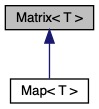
\includegraphics[width=146pt]{class_matrix__inherit__graph}
\end{center}
\end{figure}
\subsection*{Public Member Functions}
\begin{DoxyCompactItemize}
\item 
\hyperlink{class_matrix_a53f60218c002f2bb454695a1fc35c5d3}{Matrix} (unsigned long rows=0, unsigned long cols=0)
\begin{DoxyCompactList}\small\item\em The standard constructor. \end{DoxyCompactList}\item 
\hyperlink{class_matrix_a3796b4f32dc8e11f908a90fd3dd39c45}{Matrix} (const \hyperlink{class_matrix}{Matrix} \&m)
\begin{DoxyCompactList}\small\item\em The copy constructor. \end{DoxyCompactList}\item 
virtual \hyperlink{class_matrix_ab8cec5fdc5a9d228e19d1d1e5ccac8cf}{$\sim$\+Matrix} ()\hypertarget{class_matrix_ab8cec5fdc5a9d228e19d1d1e5ccac8cf}{}\label{class_matrix_ab8cec5fdc5a9d228e19d1d1e5ccac8cf}

\begin{DoxyCompactList}\small\item\em The destructor. \end{DoxyCompactList}\item 
void \hyperlink{class_matrix_aa393296d4132d7aafc4e236ddfe59f06}{set\+Size} (unsigned long rows, unsigned long cols)
\begin{DoxyCompactList}\small\item\em Sets the matrix size. Similar concept to that for Rows. \end{DoxyCompactList}\item 
unsigned long \hyperlink{class_matrix_a9b4ce445c65dcea66c66dda875cc39d8}{get\+Cols} () const 
\begin{DoxyCompactList}\small\item\em Getter for the number of columns. \end{DoxyCompactList}\item 
unsigned long \hyperlink{class_matrix_a442879db6473eeab202928dc47992206}{get\+Rows} () const 
\begin{DoxyCompactList}\small\item\em Getter for the number of rows. \end{DoxyCompactList}\item 
\hyperlink{class_row}{Row}$<$ T $>$ \& \hyperlink{class_matrix_ae7e14b4bd8bb570260a4e578e4a601b7}{operator\mbox{[}$\,$\mbox{]}} (unsigned long index)
\begin{DoxyCompactList}\small\item\em Overoads the \mbox{[}\mbox{]} operator for \hyperlink{class_matrix}{Matrix}. Allows referencing of a value i,j using \hyperlink{class_matrix}{Matrix}\mbox{[}i\mbox{]}\mbox{[}j\mbox{]}. Includes error checking for if the indices are out of range of the matrix. Note that this functionality has been altered since the original file generation. \end{DoxyCompactList}\item 
\hyperlink{class_matrix}{Matrix} \& \hyperlink{class_matrix_a94508f84ba0d62e81aa8d508aa43f1ec}{operator=} (const \hyperlink{class_matrix}{Matrix} \&m)
\begin{DoxyCompactList}\small\item\em Overloading the = operator. \end{DoxyCompactList}\item 
\hyperlink{class_matrix}{Matrix} \hyperlink{class_matrix_abdbd1bbdae2f6926cdc2b58faa304826}{operator+} (const \hyperlink{class_matrix}{Matrix} \&m) const 
\begin{DoxyCompactList}\small\item\em Overloading the + operator. \end{DoxyCompactList}\item 
\hyperlink{class_matrix}{Matrix} \hyperlink{class_matrix_a73b8da7142ea2593ba7d097651a3ce5c}{operator-\/} (const \hyperlink{class_matrix}{Matrix} \&m) const 
\begin{DoxyCompactList}\small\item\em Overloading the -\/ operator. \end{DoxyCompactList}\item 
\hyperlink{class_matrix}{Matrix} \& \hyperlink{class_matrix_a480a72298ae1fc8443b0edfaa66d7c46}{operator+=} (const \hyperlink{class_matrix}{Matrix} \&m)
\begin{DoxyCompactList}\small\item\em Overloading the += operator so that the new object is written to the current object. \end{DoxyCompactList}\item 
\hyperlink{class_matrix}{Matrix} \& \hyperlink{class_matrix_a0e459fd035b2435ea016dc93c55ccac0}{operator-\/=} (const \hyperlink{class_matrix}{Matrix} \&m)
\begin{DoxyCompactList}\small\item\em Overloading the -\/= operator so that the new object is written to the current object. \end{DoxyCompactList}\item 
\hyperlink{class_matrix}{Matrix} \hyperlink{class_matrix_a7285ecf2cfdfdcf3a3e19b4cde235528}{operator$\ast$} (const double s) const 
\begin{DoxyCompactList}\small\item\em Overloading the $\ast$ operator for scaling. \end{DoxyCompactList}\item 
\hyperlink{class_matrix}{Matrix} \hyperlink{class_matrix_a965f8987b92cfdbf8f17d3cf1bf0fa9b}{operator$\ast$} (\hyperlink{class_matrix}{Matrix} \&m) const 
\begin{DoxyCompactList}\small\item\em Overloading the $\ast$ operator for matrix multiplication. Multiplies each value in the matrix with its corresponding value in the other matrix. \end{DoxyCompactList}\item 
void \hyperlink{class_matrix_ae511e2f5874e7602fc968541efeefca1}{set\+Value} (const unsigned long \&x, const unsigned long \&y, const char $\ast$value)
\begin{DoxyCompactList}\small\item\em Sets the value at the specified indices, including handling type conversion from char to the template class. \end{DoxyCompactList}\item 
virtual void \hyperlink{class_matrix_a2476517be70c810ad586d0f0cf4ec121}{import} (const string \&filename)
\begin{DoxyCompactList}\small\item\em Imports the matrix from a csv file. \end{DoxyCompactList}\item 
bool \hyperlink{class_matrix_a0a5d9135e9807b81ddc3cf05e777a902}{import\+Csv} (const string \&filename)
\begin{DoxyCompactList}\small\item\em Imports the matrix from a csv file using the fast-\/csv-\/parser method. \end{DoxyCompactList}\end{DoxyCompactItemize}
\subsection*{Protected Attributes}
\begin{DoxyCompactItemize}
\item 
unsigned long {\bfseries num\+Cols} \{\}\hypertarget{class_matrix_a341aaedcfaac978957087bd0467dc527}{}\label{class_matrix_a341aaedcfaac978957087bd0467dc527}

\item 
unsigned long {\bfseries num\+Rows} \{\}\hypertarget{class_matrix_ac1e96667d48c7845708f978ddd17475d}{}\label{class_matrix_ac1e96667d48c7845708f978ddd17475d}

\item 
\hyperlink{class_row}{Row}$<$ T $>$ $\ast$ {\bfseries matrix}\hypertarget{class_matrix_a7a143ae112112155c9622ba17dc434c7}{}\label{class_matrix_a7a143ae112112155c9622ba17dc434c7}

\end{DoxyCompactItemize}
\subsection*{Friends}
\begin{DoxyCompactItemize}
\item 
ostream \& \hyperlink{class_matrix_ab3d577ddd4221a3da49296c2c4ae4e04}{write\+Out} (ostream \&os, const \hyperlink{class_matrix}{Matrix} \&m)
\begin{DoxyCompactList}\small\item\em Writes the object to the output stream. \end{DoxyCompactList}\item 
istream \& \hyperlink{class_matrix_a7518cae16b9081c23c94b77b6d84e0d8}{read\+In} (istream \&is, \hyperlink{class_matrix}{Matrix} \&m)
\begin{DoxyCompactList}\small\item\em Reads in from the input stream. \end{DoxyCompactList}\item 
ostream \& \hyperlink{class_matrix_a5ed9a90fd6f010e7e9840a17d92d5361}{operator$<$$<$} (ostream \&os, const \hyperlink{class_matrix}{Matrix} \&m)
\begin{DoxyCompactList}\small\item\em Overloading the $<$$<$ operator for outputting to an output stream. This can be used for writing to console or storing to file. \end{DoxyCompactList}\item 
istream \& \hyperlink{class_matrix_afcea9fa7d9a5052070fe1fda963ef237}{operator$>$$>$} (istream \&is, \hyperlink{class_matrix}{Matrix} \&m)
\begin{DoxyCompactList}\small\item\em Overloading the $>$$>$ operator for inputting from an input stream. This can be used for writing to console or storing to file. \end{DoxyCompactList}\end{DoxyCompactItemize}


\subsection{Detailed Description}
\subsubsection*{template$<$class T$>$\\*
class Matrix$<$ T $>$}

A class containing the \hyperlink{class_matrix}{Matrix} object, set up as an array of \hyperlink{class_row}{Row} objects. Includes basic operations, as well as the \hyperlink{class_matrix_a0a5d9135e9807b81ddc3cf05e777a902}{import\+Csv()} function for more advanced reading from file. 


\begin{DoxyTemplParams}{Template Parameters}
{\em T} & the type of the values in the matrix \\
\hline
\end{DoxyTemplParams}


\subsection{Constructor \& Destructor Documentation}
\index{Matrix@{Matrix}!Matrix@{Matrix}}
\index{Matrix@{Matrix}!Matrix@{Matrix}}
\subsubsection[{\texorpdfstring{Matrix(unsigned long rows=0, unsigned long cols=0)}{Matrix(unsigned long rows=0, unsigned long cols=0)}}]{\setlength{\rightskip}{0pt plus 5cm}template$<$class T$>$ {\bf Matrix}$<$ T $>$\+::{\bf Matrix} (
\begin{DoxyParamCaption}
\item[{unsigned long}]{rows = {\ttfamily 0}, }
\item[{unsigned long}]{cols = {\ttfamily 0}}
\end{DoxyParamCaption}
)\hspace{0.3cm}{\ttfamily [inline]}, {\ttfamily [explicit]}}\hypertarget{class_matrix_a53f60218c002f2bb454695a1fc35c5d3}{}\label{class_matrix_a53f60218c002f2bb454695a1fc35c5d3}


The standard constructor. 


\begin{DoxyParams}{Parameters}
{\em rows} & optionally provide the number of rows. \\
\hline
{\em cols} & optionally provide the number of columns. \\
\hline
\end{DoxyParams}
\index{Matrix@{Matrix}!Matrix@{Matrix}}
\index{Matrix@{Matrix}!Matrix@{Matrix}}
\subsubsection[{\texorpdfstring{Matrix(const Matrix \&m)}{Matrix(const Matrix &m)}}]{\setlength{\rightskip}{0pt plus 5cm}template$<$class T$>$ {\bf Matrix}$<$ T $>$\+::{\bf Matrix} (
\begin{DoxyParamCaption}
\item[{const {\bf Matrix}$<$ T $>$ \&}]{m}
\end{DoxyParamCaption}
)\hspace{0.3cm}{\ttfamily [inline]}}\hypertarget{class_matrix_a3796b4f32dc8e11f908a90fd3dd39c45}{}\label{class_matrix_a3796b4f32dc8e11f908a90fd3dd39c45}


The copy constructor. 


\begin{DoxyParams}{Parameters}
{\em m} & a \hyperlink{class_matrix}{Matrix} object to copy from. \\
\hline
\end{DoxyParams}


\subsection{Member Function Documentation}
\index{Matrix@{Matrix}!get\+Cols@{get\+Cols}}
\index{get\+Cols@{get\+Cols}!Matrix@{Matrix}}
\subsubsection[{\texorpdfstring{get\+Cols() const }{getCols() const }}]{\setlength{\rightskip}{0pt plus 5cm}template$<$class T$>$ unsigned long {\bf Matrix}$<$ T $>$\+::get\+Cols (
\begin{DoxyParamCaption}
{}
\end{DoxyParamCaption}
) const\hspace{0.3cm}{\ttfamily [inline]}}\hypertarget{class_matrix_a9b4ce445c65dcea66c66dda875cc39d8}{}\label{class_matrix_a9b4ce445c65dcea66c66dda875cc39d8}


Getter for the number of columns. 

\begin{DoxyReturn}{Returns}
the number of columns. 
\end{DoxyReturn}
\index{Matrix@{Matrix}!get\+Rows@{get\+Rows}}
\index{get\+Rows@{get\+Rows}!Matrix@{Matrix}}
\subsubsection[{\texorpdfstring{get\+Rows() const }{getRows() const }}]{\setlength{\rightskip}{0pt plus 5cm}template$<$class T$>$ unsigned long {\bf Matrix}$<$ T $>$\+::get\+Rows (
\begin{DoxyParamCaption}
{}
\end{DoxyParamCaption}
) const\hspace{0.3cm}{\ttfamily [inline]}}\hypertarget{class_matrix_a442879db6473eeab202928dc47992206}{}\label{class_matrix_a442879db6473eeab202928dc47992206}


Getter for the number of rows. 

\begin{DoxyReturn}{Returns}
the number of rows. 
\end{DoxyReturn}
\index{Matrix@{Matrix}!import@{import}}
\index{import@{import}!Matrix@{Matrix}}
\subsubsection[{\texorpdfstring{import(const string \&filename)}{import(const string &filename)}}]{\setlength{\rightskip}{0pt plus 5cm}template$<$class T$>$ virtual void {\bf Matrix}$<$ T $>$\+::import (
\begin{DoxyParamCaption}
\item[{const string \&}]{filename}
\end{DoxyParamCaption}
)\hspace{0.3cm}{\ttfamily [inline]}, {\ttfamily [virtual]}}\hypertarget{class_matrix_a2476517be70c810ad586d0f0cf4ec121}{}\label{class_matrix_a2476517be70c810ad586d0f0cf4ec121}


Imports the matrix from a csv file. 


\begin{DoxyExceptions}{Exceptions}
{\em runtime\+\_\+error} & if type detection for the filename fails. \\
\hline
\end{DoxyExceptions}

\begin{DoxyParams}{Parameters}
{\em filename} & the file to import. \\
\hline
\end{DoxyParams}


Reimplemented in \hyperlink{class_map_ad1a25204dce37addc3453e091552b014}{Map$<$ T $>$}, \hyperlink{class_map_ad1a25204dce37addc3453e091552b014}{Map$<$ uint32\+\_\+t $>$}, \hyperlink{class_map_ad1a25204dce37addc3453e091552b014}{Map$<$ double $>$}, and \hyperlink{class_map_ad1a25204dce37addc3453e091552b014}{Map$<$ bool $>$}.

\index{Matrix@{Matrix}!import\+Csv@{import\+Csv}}
\index{import\+Csv@{import\+Csv}!Matrix@{Matrix}}
\subsubsection[{\texorpdfstring{import\+Csv(const string \&filename)}{importCsv(const string &filename)}}]{\setlength{\rightskip}{0pt plus 5cm}template$<$class T$>$ bool {\bf Matrix}$<$ T $>$\+::import\+Csv (
\begin{DoxyParamCaption}
\item[{const string \&}]{filename}
\end{DoxyParamCaption}
)\hspace{0.3cm}{\ttfamily [inline]}}\hypertarget{class_matrix_a0a5d9135e9807b81ddc3cf05e777a902}{}\label{class_matrix_a0a5d9135e9807b81ddc3cf05e777a902}


Imports the matrix from a csv file using the fast-\/csv-\/parser method. 


\begin{DoxyParams}{Parameters}
{\em filename} & the path to the file to import. Imports the matrix from a csv file using the standard, slower method. \\
\hline
\end{DoxyParams}
\begin{DoxyRefDesc}{Deprecated}
\item[\hyperlink{deprecated__deprecated000003}{Deprecated}]this function should not be used any more as it is much slower. \end{DoxyRefDesc}

\begin{DoxyParams}{Parameters}
{\em filename} & the path to the file to import. \\
\hline
\end{DoxyParams}
\begin{DoxyReturn}{Returns}
true if the csv can be imported. 
\end{DoxyReturn}
\index{Matrix@{Matrix}!operator$\ast$@{operator$\ast$}}
\index{operator$\ast$@{operator$\ast$}!Matrix@{Matrix}}
\subsubsection[{\texorpdfstring{operator$\ast$(const double s) const }{operator*(const double s) const }}]{\setlength{\rightskip}{0pt plus 5cm}template$<$class T$>$ {\bf Matrix} {\bf Matrix}$<$ T $>$\+::operator$\ast$ (
\begin{DoxyParamCaption}
\item[{const double}]{s}
\end{DoxyParamCaption}
) const\hspace{0.3cm}{\ttfamily [inline]}}\hypertarget{class_matrix_a7285ecf2cfdfdcf3a3e19b4cde235528}{}\label{class_matrix_a7285ecf2cfdfdcf3a3e19b4cde235528}


Overloading the $\ast$ operator for scaling. 


\begin{DoxyParams}{Parameters}
{\em s} & the constant to scale the matrix by. \\
\hline
\end{DoxyParams}
\begin{DoxyReturn}{Returns}
the scaled matrix. 
\end{DoxyReturn}
\index{Matrix@{Matrix}!operator$\ast$@{operator$\ast$}}
\index{operator$\ast$@{operator$\ast$}!Matrix@{Matrix}}
\subsubsection[{\texorpdfstring{operator$\ast$(\+Matrix \&m) const }{operator*(Matrix &m) const }}]{\setlength{\rightskip}{0pt plus 5cm}template$<$class T$>$ {\bf Matrix} {\bf Matrix}$<$ T $>$\+::operator$\ast$ (
\begin{DoxyParamCaption}
\item[{{\bf Matrix}$<$ T $>$ \&}]{m}
\end{DoxyParamCaption}
) const\hspace{0.3cm}{\ttfamily [inline]}}\hypertarget{class_matrix_a965f8987b92cfdbf8f17d3cf1bf0fa9b}{}\label{class_matrix_a965f8987b92cfdbf8f17d3cf1bf0fa9b}


Overloading the $\ast$ operator for matrix multiplication. Multiplies each value in the matrix with its corresponding value in the other matrix. 


\begin{DoxyParams}{Parameters}
{\em m} & the matrix to multiply with \\
\hline
\end{DoxyParams}
\begin{DoxyReturn}{Returns}
the product of each ith,jth value of the matrix. 
\end{DoxyReturn}
\index{Matrix@{Matrix}!operator+@{operator+}}
\index{operator+@{operator+}!Matrix@{Matrix}}
\subsubsection[{\texorpdfstring{operator+(const Matrix \&m) const }{operator+(const Matrix &m) const }}]{\setlength{\rightskip}{0pt plus 5cm}template$<$class T$>$ {\bf Matrix} {\bf Matrix}$<$ T $>$\+::operator+ (
\begin{DoxyParamCaption}
\item[{const {\bf Matrix}$<$ T $>$ \&}]{m}
\end{DoxyParamCaption}
) const\hspace{0.3cm}{\ttfamily [inline]}}\hypertarget{class_matrix_abdbd1bbdae2f6926cdc2b58faa304826}{}\label{class_matrix_abdbd1bbdae2f6926cdc2b58faa304826}


Overloading the + operator. 


\begin{DoxyParams}{Parameters}
{\em m} & the matrix to add to this matrix. \\
\hline
\end{DoxyParams}
\begin{DoxyReturn}{Returns}
the matrix object which is the sum of the two matrices. 
\end{DoxyReturn}
\index{Matrix@{Matrix}!operator+=@{operator+=}}
\index{operator+=@{operator+=}!Matrix@{Matrix}}
\subsubsection[{\texorpdfstring{operator+=(const Matrix \&m)}{operator+=(const Matrix &m)}}]{\setlength{\rightskip}{0pt plus 5cm}template$<$class T$>$ {\bf Matrix}\& {\bf Matrix}$<$ T $>$\+::operator+= (
\begin{DoxyParamCaption}
\item[{const {\bf Matrix}$<$ T $>$ \&}]{m}
\end{DoxyParamCaption}
)\hspace{0.3cm}{\ttfamily [inline]}}\hypertarget{class_matrix_a480a72298ae1fc8443b0edfaa66d7c46}{}\label{class_matrix_a480a72298ae1fc8443b0edfaa66d7c46}


Overloading the += operator so that the new object is written to the current object. 


\begin{DoxyParams}{Parameters}
{\em m} & the \hyperlink{class_matrix}{Matrix} object to add to this matrix. \\
\hline
\end{DoxyParams}
\index{Matrix@{Matrix}!operator-\/@{operator-\/}}
\index{operator-\/@{operator-\/}!Matrix@{Matrix}}
\subsubsection[{\texorpdfstring{operator-\/(const Matrix \&m) const }{operator-(const Matrix &m) const }}]{\setlength{\rightskip}{0pt plus 5cm}template$<$class T$>$ {\bf Matrix} {\bf Matrix}$<$ T $>$\+::operator-\/ (
\begin{DoxyParamCaption}
\item[{const {\bf Matrix}$<$ T $>$ \&}]{m}
\end{DoxyParamCaption}
) const\hspace{0.3cm}{\ttfamily [inline]}}\hypertarget{class_matrix_a73b8da7142ea2593ba7d097651a3ce5c}{}\label{class_matrix_a73b8da7142ea2593ba7d097651a3ce5c}


Overloading the -\/ operator. 


\begin{DoxyParams}{Parameters}
{\em m} & the matrix to subtract from this matrix. \\
\hline
\end{DoxyParams}
\begin{DoxyReturn}{Returns}
the matrix object which is the subtraction of the two matrices. 
\end{DoxyReturn}
\index{Matrix@{Matrix}!operator-\/=@{operator-\/=}}
\index{operator-\/=@{operator-\/=}!Matrix@{Matrix}}
\subsubsection[{\texorpdfstring{operator-\/=(const Matrix \&m)}{operator-=(const Matrix &m)}}]{\setlength{\rightskip}{0pt plus 5cm}template$<$class T$>$ {\bf Matrix}\& {\bf Matrix}$<$ T $>$\+::operator-\/= (
\begin{DoxyParamCaption}
\item[{const {\bf Matrix}$<$ T $>$ \&}]{m}
\end{DoxyParamCaption}
)\hspace{0.3cm}{\ttfamily [inline]}}\hypertarget{class_matrix_a0e459fd035b2435ea016dc93c55ccac0}{}\label{class_matrix_a0e459fd035b2435ea016dc93c55ccac0}


Overloading the -\/= operator so that the new object is written to the current object. 


\begin{DoxyParams}{Parameters}
{\em m} & the \hyperlink{class_matrix}{Matrix} object to subtract from this matrix. \\
\hline
\end{DoxyParams}
\index{Matrix@{Matrix}!operator=@{operator=}}
\index{operator=@{operator=}!Matrix@{Matrix}}
\subsubsection[{\texorpdfstring{operator=(const Matrix \&m)}{operator=(const Matrix &m)}}]{\setlength{\rightskip}{0pt plus 5cm}template$<$class T$>$ {\bf Matrix}\& {\bf Matrix}$<$ T $>$\+::operator= (
\begin{DoxyParamCaption}
\item[{const {\bf Matrix}$<$ T $>$ \&}]{m}
\end{DoxyParamCaption}
)\hspace{0.3cm}{\ttfamily [inline]}}\hypertarget{class_matrix_a94508f84ba0d62e81aa8d508aa43f1ec}{}\label{class_matrix_a94508f84ba0d62e81aa8d508aa43f1ec}


Overloading the = operator. 


\begin{DoxyParams}{Parameters}
{\em m} & the matrix to copy from. \\
\hline
\end{DoxyParams}
\index{Matrix@{Matrix}!operator\mbox{[}$\,$\mbox{]}@{operator[]}}
\index{operator\mbox{[}$\,$\mbox{]}@{operator[]}!Matrix@{Matrix}}
\subsubsection[{\texorpdfstring{operator[](unsigned long index)}{operator[](unsigned long index)}}]{\setlength{\rightskip}{0pt plus 5cm}template$<$class T$>$ {\bf Row}$<$T$>$\& {\bf Matrix}$<$ T $>$\+::operator\mbox{[}$\,$\mbox{]} (
\begin{DoxyParamCaption}
\item[{unsigned long}]{index}
\end{DoxyParamCaption}
)\hspace{0.3cm}{\ttfamily [inline]}}\hypertarget{class_matrix_ae7e14b4bd8bb570260a4e578e4a601b7}{}\label{class_matrix_ae7e14b4bd8bb570260a4e578e4a601b7}


Overoads the \mbox{[}\mbox{]} operator for \hyperlink{class_matrix}{Matrix}. Allows referencing of a value i,j using \hyperlink{class_matrix}{Matrix}\mbox{[}i\mbox{]}\mbox{[}j\mbox{]}. Includes error checking for if the indices are out of range of the matrix. Note that this functionality has been altered since the original file generation. 


\begin{DoxyParams}{Parameters}
{\em index} & the row number to get the value from. \\
\hline
\end{DoxyParams}
\begin{DoxyReturn}{Returns}
the matrix row object. 
\end{DoxyReturn}
\index{Matrix@{Matrix}!set\+Size@{set\+Size}}
\index{set\+Size@{set\+Size}!Matrix@{Matrix}}
\subsubsection[{\texorpdfstring{set\+Size(unsigned long rows, unsigned long cols)}{setSize(unsigned long rows, unsigned long cols)}}]{\setlength{\rightskip}{0pt plus 5cm}template$<$class T$>$ void {\bf Matrix}$<$ T $>$\+::set\+Size (
\begin{DoxyParamCaption}
\item[{unsigned long}]{rows, }
\item[{unsigned long}]{cols}
\end{DoxyParamCaption}
)\hspace{0.3cm}{\ttfamily [inline]}}\hypertarget{class_matrix_aa393296d4132d7aafc4e236ddfe59f06}{}\label{class_matrix_aa393296d4132d7aafc4e236ddfe59f06}


Sets the matrix size. Similar concept to that for Rows. 


\begin{DoxyParams}{Parameters}
{\em rows} & the number of rows. \\
\hline
{\em cols} & the number of columns. \\
\hline
\end{DoxyParams}
\index{Matrix@{Matrix}!set\+Value@{set\+Value}}
\index{set\+Value@{set\+Value}!Matrix@{Matrix}}
\subsubsection[{\texorpdfstring{set\+Value(const unsigned long \&x, const unsigned long \&y, const char $\ast$value)}{setValue(const unsigned long &x, const unsigned long &y, const char *value)}}]{\setlength{\rightskip}{0pt plus 5cm}template$<$class T$>$ void {\bf Matrix}$<$ T $>$\+::set\+Value (
\begin{DoxyParamCaption}
\item[{const unsigned long \&}]{x, }
\item[{const unsigned long \&}]{y, }
\item[{const char $\ast$}]{value}
\end{DoxyParamCaption}
)\hspace{0.3cm}{\ttfamily [inline]}}\hypertarget{class_matrix_ae511e2f5874e7602fc968541efeefca1}{}\label{class_matrix_ae511e2f5874e7602fc968541efeefca1}


Sets the value at the specified indices, including handling type conversion from char to the template class. 


\begin{DoxyParams}{Parameters}
{\em x} & the x index. \\
\hline
{\em y} & the y index. \\
\hline
{\em value} & the value to set \\
\hline
\end{DoxyParams}


\subsection{Friends And Related Function Documentation}
\index{Matrix@{Matrix}!operator$<$$<$@{operator$<$$<$}}
\index{operator$<$$<$@{operator$<$$<$}!Matrix@{Matrix}}
\subsubsection[{\texorpdfstring{operator$<$$<$}{operator<<}}]{\setlength{\rightskip}{0pt plus 5cm}template$<$class T$>$ ostream\& operator$<$$<$ (
\begin{DoxyParamCaption}
\item[{ostream \&}]{os, }
\item[{const {\bf Matrix}$<$ T $>$ \&}]{m}
\end{DoxyParamCaption}
)\hspace{0.3cm}{\ttfamily [friend]}}\hypertarget{class_matrix_a5ed9a90fd6f010e7e9840a17d92d5361}{}\label{class_matrix_a5ed9a90fd6f010e7e9840a17d92d5361}


Overloading the $<$$<$ operator for outputting to an output stream. This can be used for writing to console or storing to file. 


\begin{DoxyParams}{Parameters}
{\em os} & the output stream. \\
\hline
{\em m} & the matrix to output. \\
\hline
\end{DoxyParams}
\begin{DoxyReturn}{Returns}
the output stream. 
\end{DoxyReturn}
\index{Matrix@{Matrix}!operator$>$$>$@{operator$>$$>$}}
\index{operator$>$$>$@{operator$>$$>$}!Matrix@{Matrix}}
\subsubsection[{\texorpdfstring{operator$>$$>$}{operator>>}}]{\setlength{\rightskip}{0pt plus 5cm}template$<$class T$>$ istream\& operator$>$$>$ (
\begin{DoxyParamCaption}
\item[{istream \&}]{is, }
\item[{{\bf Matrix}$<$ T $>$ \&}]{m}
\end{DoxyParamCaption}
)\hspace{0.3cm}{\ttfamily [friend]}}\hypertarget{class_matrix_afcea9fa7d9a5052070fe1fda963ef237}{}\label{class_matrix_afcea9fa7d9a5052070fe1fda963ef237}


Overloading the $>$$>$ operator for inputting from an input stream. This can be used for writing to console or storing to file. 


\begin{DoxyParams}{Parameters}
{\em is} & the input stream. \\
\hline
{\em m} & the matrix to input to. \\
\hline
\end{DoxyParams}
\begin{DoxyReturn}{Returns}
the input stream. 
\end{DoxyReturn}
\index{Matrix@{Matrix}!read\+In@{read\+In}}
\index{read\+In@{read\+In}!Matrix@{Matrix}}
\subsubsection[{\texorpdfstring{read\+In}{readIn}}]{\setlength{\rightskip}{0pt plus 5cm}template$<$class T$>$ istream\& read\+In (
\begin{DoxyParamCaption}
\item[{istream \&}]{is, }
\item[{{\bf Matrix}$<$ T $>$ \&}]{m}
\end{DoxyParamCaption}
)\hspace{0.3cm}{\ttfamily [friend]}}\hypertarget{class_matrix_a7518cae16b9081c23c94b77b6d84e0d8}{}\label{class_matrix_a7518cae16b9081c23c94b77b6d84e0d8}


Reads in from the input stream. 


\begin{DoxyParams}{Parameters}
{\em is} & the input stream to read from \\
\hline
{\em m} & the object to read into \\
\hline
\end{DoxyParams}
\begin{DoxyReturn}{Returns}

\end{DoxyReturn}
\index{Matrix@{Matrix}!write\+Out@{write\+Out}}
\index{write\+Out@{write\+Out}!Matrix@{Matrix}}
\subsubsection[{\texorpdfstring{write\+Out}{writeOut}}]{\setlength{\rightskip}{0pt plus 5cm}template$<$class T$>$ ostream\& write\+Out (
\begin{DoxyParamCaption}
\item[{ostream \&}]{os, }
\item[{const {\bf Matrix}$<$ T $>$ \&}]{m}
\end{DoxyParamCaption}
)\hspace{0.3cm}{\ttfamily [friend]}}\hypertarget{class_matrix_ab3d577ddd4221a3da49296c2c4ae4e04}{}\label{class_matrix_ab3d577ddd4221a3da49296c2c4ae4e04}


Writes the object to the output stream. 


\begin{DoxyParams}{Parameters}
{\em os} & the output stream to write to \\
\hline
{\em m} & the object to write out \\
\hline
\end{DoxyParams}
\begin{DoxyReturn}{Returns}
the output stream 
\end{DoxyReturn}


The documentation for this class was generated from the following file\+:\begin{DoxyCompactItemize}
\item 
necsim/Matrix.\+h\end{DoxyCompactItemize}

\hypertarget{structmodule__state}{}\section{module\+\_\+state Struct Reference}
\label{structmodule__state}\index{module\+\_\+state@{module\+\_\+state}}
\subsection*{Public Attributes}
\begin{DoxyCompactItemize}
\item 
Py\+Object $\ast$ {\bfseries error}\hypertarget{structmodule__state_a6593da300121fe46fad3e7280053fab8}{}\label{structmodule__state_a6593da300121fe46fad3e7280053fab8}

\end{DoxyCompactItemize}


The documentation for this struct was generated from the following files\+:\begin{DoxyCompactItemize}
\item 
\hyperlink{applyspecmodule_8h}{applyspecmodule.\+h}\item 
\hyperlink{dispersalmodule_8h}{dispersalmodule.\+h}\item 
\hyperlink{necsimmodule_8h}{necsimmodule.\+h}\end{DoxyCompactItemize}

\hypertarget{class_n_rrand}{}\section{N\+Rrand Class Reference}
\label{class_n_rrand}\index{N\+Rrand@{N\+Rrand}}


Contains the functions for random number generation.  




{\ttfamily \#include $<$N\+Rrand.\+h$>$}

\subsection*{Public Member Functions}
\begin{DoxyCompactItemize}
\item 
\hyperlink{class_n_rrand_a674521c4c29a6cb692f343ea9cf6a40c}{N\+Rrand} ()\hypertarget{class_n_rrand_a674521c4c29a6cb692f343ea9cf6a40c}{}\label{class_n_rrand_a674521c4c29a6cb692f343ea9cf6a40c}

\begin{DoxyCompactList}\small\item\em Standard constructor. \end{DoxyCompactList}\item 
void \hyperlink{class_n_rrand_a23325b4d35ee0b5b580726db05e2b8a3}{set\+Seed} (long seed)
\begin{DoxyCompactList}\small\item\em Sets the seed to the given input. Is only seeded if the seed hasn\textquotesingle{}t already been provided. \end{DoxyCompactList}\item 
double \hyperlink{class_n_rrand_a0043ba1c33b3dcb3b98210fb432f9f6c}{d01} ()
\begin{DoxyCompactList}\small\item\em The random number generator. Uses Schrage\textquotesingle{}s method and a shuffle table to generate the output. \end{DoxyCompactList}\item 
unsigned long \hyperlink{class_n_rrand_abb6db53dd1fdd9388b39e5dcd26c13ac}{i0} (unsigned long max)
\begin{DoxyCompactList}\small\item\em Generates a random number uniformly from 0 to the maximum value provided. \end{DoxyCompactList}\item 
double \hyperlink{class_n_rrand_aa57a6e9bae94c2df5a00473ba6fa900d}{norm} ()
\begin{DoxyCompactList}\small\item\em Generates a normally distributed number Uses the standard normal distribution from a Box-\/\+Muller transform. \end{DoxyCompactList}\item 
double \hyperlink{class_n_rrand_a754e5083299d12c1b33e8c66519d057e}{norm2D} ()
\begin{DoxyCompactList}\small\item\em Returns a 2 dimensional call from a normal distribution, giving a distance in cartesian space This way is slightly inefficient for normal distributions, but it\textquotesingle{}s kept this way to make the \hyperlink{class_map_a7c5b0623134a33511d7c17626c967176}{Map\+::run\+Dispersal()} function applicable with any dispersal type. \end{DoxyCompactList}\item 
void \hyperlink{class_n_rrand_a5679f458940de730f527772ca27db5ad}{set\+Dispersal\+Params} (const double sigmain, const double tauin)
\begin{DoxyCompactList}\small\item\em Sets the dispersal parameters, avoiding requirement to provide these numbers each function call. This is only relevant for fat-\/tailed dispersal calls. \end{DoxyCompactList}\item 
double \hyperlink{class_n_rrand_a464101f3def678477f9156d0bd1aab54}{fattail} (double z)
\begin{DoxyCompactList}\small\item\em Call from the fat-\/tailed dispersal kernel with the provided sigma. \end{DoxyCompactList}\item 
double \hyperlink{class_n_rrand_a3ec8aae87ae486ddfb5ad481a7972c27}{fattail} ()
\begin{DoxyCompactList}\small\item\em Call from fat-\/tailed dispersal kernel. This function requires \hyperlink{class_n_rrand_a5679f458940de730f527772ca27db5ad}{set\+Dispersal\+Params()} has already been called. \end{DoxyCompactList}\item 
double \hyperlink{class_n_rrand_aab0ec97e2c0f74cf38cc7047356cae5c}{fattail\+\_\+old} ()
\begin{DoxyCompactList}\small\item\em Old version of the function call reparameterised for different nu and sigma. \end{DoxyCompactList}\item 
double \hyperlink{class_n_rrand_aef021289f62893215204589af450bf65}{direction} ()
\begin{DoxyCompactList}\small\item\em Generates a direction in radians. \end{DoxyCompactList}\item 
bool \hyperlink{class_n_rrand_a7c7a2dc1b3f14ebaaa0e6edd6c1d517a}{event} (double event\+\_\+probability)
\begin{DoxyCompactList}\small\item\em For a given event probability, returns the probability that the event has occured. \end{DoxyCompactList}\item 
double \hyperlink{class_n_rrand_ab18277b2f873878602e82672b272c9be}{norm\+Uniform} ()
\begin{DoxyCompactList}\small\item\em Normal distribution, with percentage chance to choose a uniform distribution instead. \end{DoxyCompactList}\item 
double \hyperlink{class_n_rrand_a799f55c57dc238f094a20e882e3abb51}{uniform\+Uniform} ()
\begin{DoxyCompactList}\small\item\em Two uniform distributions, the first between 0 and 0.\+1$\ast$cutoff, and the second between 0.\+9$\ast$cutoff and cutoff. Selects from both distributions equally. \end{DoxyCompactList}\item 
void \hyperlink{class_n_rrand_a432b648073ccd3cb7f8215bb5c299619}{set\+Dispersal\+Method} (const string \&dispersal\+\_\+method, const double \&m\+\_\+probin, const double \&cutoffin)
\begin{DoxyCompactList}\small\item\em Sets the dispersal method by creating the link between dispersal\+Function() and the correct dispersal character. \end{DoxyCompactList}\item 
double \hyperlink{class_n_rrand_a1e15746ff8398488245b750325f37b08}{dispersal} ()
\begin{DoxyCompactList}\small\item\em Runs the dispersal with the allocated dispersal function. \end{DoxyCompactList}\end{DoxyCompactItemize}
\subsection*{Friends}
\begin{DoxyCompactItemize}
\item 
ostream \& \hyperlink{class_n_rrand_a604ebc1c878ab63df21e123dbd34185f}{operator$<$$<$} (ostream \&os, const \hyperlink{class_n_rrand}{N\+Rrand} \&r)
\begin{DoxyCompactList}\small\item\em Outputs the \hyperlink{class_n_rrand}{N\+Rrand} object to the output stream. Used for saving the object to file. \end{DoxyCompactList}\item 
istream \& \hyperlink{class_n_rrand_a0b8544414e90bb92ba90afa881b1f06e}{operator$>$$>$} (istream \&is, \hyperlink{class_n_rrand}{N\+Rrand} \&r)
\begin{DoxyCompactList}\small\item\em Inputs the \hyperlink{class_n_rrand}{N\+Rrand} object from the input stream. Used for reading the \hyperlink{class_n_rrand}{N\+Rrand} object from a file. \end{DoxyCompactList}\end{DoxyCompactItemize}


\subsection{Detailed Description}
Contains the functions for random number generation. 

\subsection{Member Function Documentation}
\index{N\+Rrand@{N\+Rrand}!d01@{d01}}
\index{d01@{d01}!N\+Rrand@{N\+Rrand}}
\subsubsection[{\texorpdfstring{d01()}{d01()}}]{\setlength{\rightskip}{0pt plus 5cm}double N\+Rrand\+::d01 (
\begin{DoxyParamCaption}
{}
\end{DoxyParamCaption}
)\hspace{0.3cm}{\ttfamily [inline]}}\hypertarget{class_n_rrand_a0043ba1c33b3dcb3b98210fb432f9f6c}{}\label{class_n_rrand_a0043ba1c33b3dcb3b98210fb432f9f6c}


The random number generator. Uses Schrage\textquotesingle{}s method and a shuffle table to generate the output. 

\begin{DoxyReturn}{Returns}
the random number (a double between 0 and 1). 
\end{DoxyReturn}
\index{N\+Rrand@{N\+Rrand}!direction@{direction}}
\index{direction@{direction}!N\+Rrand@{N\+Rrand}}
\subsubsection[{\texorpdfstring{direction()}{direction()}}]{\setlength{\rightskip}{0pt plus 5cm}double N\+Rrand\+::direction (
\begin{DoxyParamCaption}
{}
\end{DoxyParamCaption}
)\hspace{0.3cm}{\ttfamily [inline]}}\hypertarget{class_n_rrand_aef021289f62893215204589af450bf65}{}\label{class_n_rrand_aef021289f62893215204589af450bf65}


Generates a direction in radians. 

\begin{DoxyReturn}{Returns}
the direction in radians 
\end{DoxyReturn}
\index{N\+Rrand@{N\+Rrand}!dispersal@{dispersal}}
\index{dispersal@{dispersal}!N\+Rrand@{N\+Rrand}}
\subsubsection[{\texorpdfstring{dispersal()}{dispersal()}}]{\setlength{\rightskip}{0pt plus 5cm}double N\+Rrand\+::dispersal (
\begin{DoxyParamCaption}
{}
\end{DoxyParamCaption}
)\hspace{0.3cm}{\ttfamily [inline]}}\hypertarget{class_n_rrand_a1e15746ff8398488245b750325f37b08}{}\label{class_n_rrand_a1e15746ff8398488245b750325f37b08}


Runs the dispersal with the allocated dispersal function. 

\begin{DoxyNote}{Note}
This function will never return a value larger than the size of L\+O\+N\+G\+\_\+\+M\+AX to avoid issues of converting doubles to integers. For dispersal distance within coalescence simulations, this is seemed a reasonable assumption, but may cause issues if code is re-\/used in later projects.
\end{DoxyNote}
\begin{DoxyReturn}{Returns}
distance the dispersal distance 
\end{DoxyReturn}
\index{N\+Rrand@{N\+Rrand}!event@{event}}
\index{event@{event}!N\+Rrand@{N\+Rrand}}
\subsubsection[{\texorpdfstring{event(double event\+\_\+probability)}{event(double event_probability)}}]{\setlength{\rightskip}{0pt plus 5cm}bool N\+Rrand\+::event (
\begin{DoxyParamCaption}
\item[{double}]{event\+\_\+probability}
\end{DoxyParamCaption}
)\hspace{0.3cm}{\ttfamily [inline]}}\hypertarget{class_n_rrand_a7c7a2dc1b3f14ebaaa0e6edd6c1d517a}{}\label{class_n_rrand_a7c7a2dc1b3f14ebaaa0e6edd6c1d517a}


For a given event probability, returns the probability that the event has occured. 


\begin{DoxyParams}{Parameters}
{\em event\+\_\+probability} & the event probability. \\
\hline
\end{DoxyParams}
\begin{DoxyReturn}{Returns}
whether or not the event has occured. 
\end{DoxyReturn}
\index{N\+Rrand@{N\+Rrand}!fattail@{fattail}}
\index{fattail@{fattail}!N\+Rrand@{N\+Rrand}}
\subsubsection[{\texorpdfstring{fattail(double z)}{fattail(double z)}}]{\setlength{\rightskip}{0pt plus 5cm}double N\+Rrand\+::fattail (
\begin{DoxyParamCaption}
\item[{double}]{z}
\end{DoxyParamCaption}
)\hspace{0.3cm}{\ttfamily [inline]}}\hypertarget{class_n_rrand_a464101f3def678477f9156d0bd1aab54}{}\label{class_n_rrand_a464101f3def678477f9156d0bd1aab54}


Call from the fat-\/tailed dispersal kernel with the provided sigma. 

\begin{DoxyRefDesc}{Deprecated}
\item[\hyperlink{deprecated__deprecated000004}{Deprecated}]This is the original version used in J Rosindell\textquotesingle{}s codebase, and has been altered for a version which approximates the gaussian distribution at extreme limits. \end{DoxyRefDesc}

\begin{DoxyParams}{Parameters}
{\em z} & the desired sigma. \\
\hline
\end{DoxyParams}
\begin{DoxyReturn}{Returns}
a random number drawn from the fat-\/tailed dispersal kernel. 
\end{DoxyReturn}
\index{N\+Rrand@{N\+Rrand}!fattail@{fattail}}
\index{fattail@{fattail}!N\+Rrand@{N\+Rrand}}
\subsubsection[{\texorpdfstring{fattail()}{fattail()}}]{\setlength{\rightskip}{0pt plus 5cm}double N\+Rrand\+::fattail (
\begin{DoxyParamCaption}
{}
\end{DoxyParamCaption}
)\hspace{0.3cm}{\ttfamily [inline]}}\hypertarget{class_n_rrand_a3ec8aae87ae486ddfb5ad481a7972c27}{}\label{class_n_rrand_a3ec8aae87ae486ddfb5ad481a7972c27}


Call from fat-\/tailed dispersal kernel. This function requires \hyperlink{class_n_rrand_a5679f458940de730f527772ca27db5ad}{set\+Dispersal\+Params()} has already been called. 

\begin{DoxyRefDesc}{Deprecated}
\item[\hyperlink{deprecated__deprecated000005}{Deprecated}]deprecated, kept for testing purposes only \end{DoxyRefDesc}
\begin{DoxyReturn}{Returns}
a random number drawn from the fat-\/tailed dispersal kernel. 
\end{DoxyReturn}
\index{N\+Rrand@{N\+Rrand}!fattail\+\_\+old@{fattail\+\_\+old}}
\index{fattail\+\_\+old@{fattail\+\_\+old}!N\+Rrand@{N\+Rrand}}
\subsubsection[{\texorpdfstring{fattail\+\_\+old()}{fattail_old()}}]{\setlength{\rightskip}{0pt plus 5cm}double N\+Rrand\+::fattail\+\_\+old (
\begin{DoxyParamCaption}
{}
\end{DoxyParamCaption}
)\hspace{0.3cm}{\ttfamily [inline]}}\hypertarget{class_n_rrand_aab0ec97e2c0f74cf38cc7047356cae5c}{}\label{class_n_rrand_aab0ec97e2c0f74cf38cc7047356cae5c}


Old version of the function call reparameterised for different nu and sigma. 

\begin{DoxyRefDesc}{Deprecated}
\item[\hyperlink{deprecated__deprecated000006}{Deprecated}]Kept only for testing purposes. \end{DoxyRefDesc}
\begin{DoxyReturn}{Returns}
a random number drawn from the fat-\/tailed dispersal kernel. 
\end{DoxyReturn}
\index{N\+Rrand@{N\+Rrand}!i0@{i0}}
\index{i0@{i0}!N\+Rrand@{N\+Rrand}}
\subsubsection[{\texorpdfstring{i0(unsigned long max)}{i0(unsigned long max)}}]{\setlength{\rightskip}{0pt plus 5cm}unsigned long N\+Rrand\+::i0 (
\begin{DoxyParamCaption}
\item[{unsigned long}]{max}
\end{DoxyParamCaption}
)\hspace{0.3cm}{\ttfamily [inline]}}\hypertarget{class_n_rrand_abb6db53dd1fdd9388b39e5dcd26c13ac}{}\label{class_n_rrand_abb6db53dd1fdd9388b39e5dcd26c13ac}


Generates a random number uniformly from 0 to the maximum value provided. 


\begin{DoxyParams}{Parameters}
{\em max} & the maximum number. \\
\hline
\end{DoxyParams}
\begin{DoxyReturn}{Returns}
an integer of the produced random number. 
\end{DoxyReturn}
\index{N\+Rrand@{N\+Rrand}!norm@{norm}}
\index{norm@{norm}!N\+Rrand@{N\+Rrand}}
\subsubsection[{\texorpdfstring{norm()}{norm()}}]{\setlength{\rightskip}{0pt plus 5cm}double N\+Rrand\+::norm (
\begin{DoxyParamCaption}
{}
\end{DoxyParamCaption}
)\hspace{0.3cm}{\ttfamily [inline]}}\hypertarget{class_n_rrand_aa57a6e9bae94c2df5a00473ba6fa900d}{}\label{class_n_rrand_aa57a6e9bae94c2df5a00473ba6fa900d}


Generates a normally distributed number Uses the standard normal distribution from a Box-\/\+Muller transform. 

\begin{DoxyReturn}{Returns}
the random number from a normal distribution. 
\end{DoxyReturn}
\index{N\+Rrand@{N\+Rrand}!norm2D@{norm2D}}
\index{norm2D@{norm2D}!N\+Rrand@{N\+Rrand}}
\subsubsection[{\texorpdfstring{norm2\+D()}{norm2D()}}]{\setlength{\rightskip}{0pt plus 5cm}double N\+Rrand\+::norm2D (
\begin{DoxyParamCaption}
{}
\end{DoxyParamCaption}
)\hspace{0.3cm}{\ttfamily [inline]}}\hypertarget{class_n_rrand_a754e5083299d12c1b33e8c66519d057e}{}\label{class_n_rrand_a754e5083299d12c1b33e8c66519d057e}


Returns a 2 dimensional call from a normal distribution, giving a distance in cartesian space This way is slightly inefficient for normal distributions, but it\textquotesingle{}s kept this way to make the \hyperlink{class_map_a7c5b0623134a33511d7c17626c967176}{Map\+::run\+Dispersal()} function applicable with any dispersal type. 

\begin{DoxyReturn}{Returns}
dispersal distance of a normal distribution 
\end{DoxyReturn}
\index{N\+Rrand@{N\+Rrand}!norm\+Uniform@{norm\+Uniform}}
\index{norm\+Uniform@{norm\+Uniform}!N\+Rrand@{N\+Rrand}}
\subsubsection[{\texorpdfstring{norm\+Uniform()}{normUniform()}}]{\setlength{\rightskip}{0pt plus 5cm}double N\+Rrand\+::norm\+Uniform (
\begin{DoxyParamCaption}
{}
\end{DoxyParamCaption}
)\hspace{0.3cm}{\ttfamily [inline]}}\hypertarget{class_n_rrand_ab18277b2f873878602e82672b272c9be}{}\label{class_n_rrand_ab18277b2f873878602e82672b272c9be}


Normal distribution, with percentage chance to choose a uniform distribution instead. 

\begin{DoxyNote}{Note}
This function will not produce the same output as \hyperlink{class_n_rrand_aa57a6e9bae94c2df5a00473ba6fa900d}{norm()} for the same parameters, even with a zero chance of picking from the uniform distribution (due to random number draws). 
\end{DoxyNote}
\begin{DoxyReturn}{Returns}
normally (or uniformly) distributed number 
\end{DoxyReturn}
\index{N\+Rrand@{N\+Rrand}!set\+Dispersal\+Method@{set\+Dispersal\+Method}}
\index{set\+Dispersal\+Method@{set\+Dispersal\+Method}!N\+Rrand@{N\+Rrand}}
\subsubsection[{\texorpdfstring{set\+Dispersal\+Method(const string \&dispersal\+\_\+method, const double \&m\+\_\+probin, const double \&cutoffin)}{setDispersalMethod(const string &dispersal_method, const double &m_probin, const double &cutoffin)}}]{\setlength{\rightskip}{0pt plus 5cm}void N\+Rrand\+::set\+Dispersal\+Method (
\begin{DoxyParamCaption}
\item[{const string \&}]{dispersal\+\_\+method, }
\item[{const double \&}]{m\+\_\+probin, }
\item[{const double \&}]{cutoffin}
\end{DoxyParamCaption}
)\hspace{0.3cm}{\ttfamily [inline]}}\hypertarget{class_n_rrand_a432b648073ccd3cb7f8215bb5c299619}{}\label{class_n_rrand_a432b648073ccd3cb7f8215bb5c299619}


Sets the dispersal method by creating the link between dispersal\+Function() and the correct dispersal character. 


\begin{DoxyParams}{Parameters}
{\em dispersal\+\_\+method} & string containing the dispersal type. Can be one of \mbox{[}normal, fat-\/tail, norm-\/uniform\mbox{]} \\
\hline
{\em m\+\_\+probin} & the probability of drawing from the uniform distribution. Only relevant for uniform dispersals. \\
\hline
{\em cutoffin} & the maximum value to be drawn from the uniform dispersal. Only relevant for uniform dispersals. \\
\hline
\end{DoxyParams}
\index{N\+Rrand@{N\+Rrand}!set\+Dispersal\+Params@{set\+Dispersal\+Params}}
\index{set\+Dispersal\+Params@{set\+Dispersal\+Params}!N\+Rrand@{N\+Rrand}}
\subsubsection[{\texorpdfstring{set\+Dispersal\+Params(const double sigmain, const double tauin)}{setDispersalParams(const double sigmain, const double tauin)}}]{\setlength{\rightskip}{0pt plus 5cm}void N\+Rrand\+::set\+Dispersal\+Params (
\begin{DoxyParamCaption}
\item[{const double}]{sigmain, }
\item[{const double}]{tauin}
\end{DoxyParamCaption}
)\hspace{0.3cm}{\ttfamily [inline]}}\hypertarget{class_n_rrand_a5679f458940de730f527772ca27db5ad}{}\label{class_n_rrand_a5679f458940de730f527772ca27db5ad}


Sets the dispersal parameters, avoiding requirement to provide these numbers each function call. This is only relevant for fat-\/tailed dispersal calls. 


\begin{DoxyParams}{Parameters}
{\em sigmain} & the fatness of the fat-\/tailed dispersal kernel. \\
\hline
{\em tauin} & the width of the fat-\/tailed dispersal kernel. \\
\hline
\end{DoxyParams}
\index{N\+Rrand@{N\+Rrand}!set\+Seed@{set\+Seed}}
\index{set\+Seed@{set\+Seed}!N\+Rrand@{N\+Rrand}}
\subsubsection[{\texorpdfstring{set\+Seed(long seed)}{setSeed(long seed)}}]{\setlength{\rightskip}{0pt plus 5cm}void N\+Rrand\+::set\+Seed (
\begin{DoxyParamCaption}
\item[{long}]{seed}
\end{DoxyParamCaption}
)\hspace{0.3cm}{\ttfamily [inline]}}\hypertarget{class_n_rrand_a23325b4d35ee0b5b580726db05e2b8a3}{}\label{class_n_rrand_a23325b4d35ee0b5b580726db05e2b8a3}


Sets the seed to the given input. Is only seeded if the seed hasn\textquotesingle{}t already been provided. 


\begin{DoxyParams}{Parameters}
{\em seed} & the input seed. \\
\hline
\end{DoxyParams}
\index{N\+Rrand@{N\+Rrand}!uniform\+Uniform@{uniform\+Uniform}}
\index{uniform\+Uniform@{uniform\+Uniform}!N\+Rrand@{N\+Rrand}}
\subsubsection[{\texorpdfstring{uniform\+Uniform()}{uniformUniform()}}]{\setlength{\rightskip}{0pt plus 5cm}double N\+Rrand\+::uniform\+Uniform (
\begin{DoxyParamCaption}
{}
\end{DoxyParamCaption}
)\hspace{0.3cm}{\ttfamily [inline]}}\hypertarget{class_n_rrand_a799f55c57dc238f094a20e882e3abb51}{}\label{class_n_rrand_a799f55c57dc238f094a20e882e3abb51}


Two uniform distributions, the first between 0 and 0.\+1$\ast$cutoff, and the second between 0.\+9$\ast$cutoff and cutoff. Selects from both distributions equally. 

\begin{DoxyNote}{Note}
The mean for this function should be identical to a uniform distribution between 0 and cutoff. 
\end{DoxyNote}
\begin{DoxyReturn}{Returns}
uniformly distributed number 
\end{DoxyReturn}


\subsection{Friends And Related Function Documentation}
\index{N\+Rrand@{N\+Rrand}!operator$<$$<$@{operator$<$$<$}}
\index{operator$<$$<$@{operator$<$$<$}!N\+Rrand@{N\+Rrand}}
\subsubsection[{\texorpdfstring{operator$<$$<$}{operator<<}}]{\setlength{\rightskip}{0pt plus 5cm}ostream\& operator$<$$<$ (
\begin{DoxyParamCaption}
\item[{ostream \&}]{os, }
\item[{const {\bf N\+Rrand} \&}]{r}
\end{DoxyParamCaption}
)\hspace{0.3cm}{\ttfamily [friend]}}\hypertarget{class_n_rrand_a604ebc1c878ab63df21e123dbd34185f}{}\label{class_n_rrand_a604ebc1c878ab63df21e123dbd34185f}


Outputs the \hyperlink{class_n_rrand}{N\+Rrand} object to the output stream. Used for saving the object to file. 


\begin{DoxyParams}{Parameters}
{\em os} & the output stream. \\
\hline
{\em r} & the \hyperlink{class_n_rrand}{N\+Rrand} object to output. \\
\hline
\end{DoxyParams}
\begin{DoxyReturn}{Returns}
the output stream. 
\end{DoxyReturn}
\index{N\+Rrand@{N\+Rrand}!operator$>$$>$@{operator$>$$>$}}
\index{operator$>$$>$@{operator$>$$>$}!N\+Rrand@{N\+Rrand}}
\subsubsection[{\texorpdfstring{operator$>$$>$}{operator>>}}]{\setlength{\rightskip}{0pt plus 5cm}istream\& operator$>$$>$ (
\begin{DoxyParamCaption}
\item[{istream \&}]{is, }
\item[{{\bf N\+Rrand} \&}]{r}
\end{DoxyParamCaption}
)\hspace{0.3cm}{\ttfamily [friend]}}\hypertarget{class_n_rrand_a0b8544414e90bb92ba90afa881b1f06e}{}\label{class_n_rrand_a0b8544414e90bb92ba90afa881b1f06e}


Inputs the \hyperlink{class_n_rrand}{N\+Rrand} object from the input stream. Used for reading the \hyperlink{class_n_rrand}{N\+Rrand} object from a file. 


\begin{DoxyParams}{Parameters}
{\em is} & the input stream. \\
\hline
{\em r} & the \hyperlink{class_n_rrand}{N\+Rrand} object to input to. \\
\hline
\end{DoxyParams}
\begin{DoxyReturn}{Returns}
the input stream. 
\end{DoxyReturn}


The documentation for this class was generated from the following file\+:\begin{DoxyCompactItemize}
\item 
necsim/N\+Rrand.\+h\end{DoxyCompactItemize}

\hypertarget{struct_previous_calc_pair}{}\section{Previous\+Calc\+Pair Struct Reference}
\label{struct_previous_calc_pair}\index{Previous\+Calc\+Pair@{Previous\+Calc\+Pair}}


A struct for containing pairs of previous calculations to make sure that aren\textquotesingle{}t repeated.  




{\ttfamily \#include $<$Treelist.\+h$>$}

\subsection*{Public Member Functions}
\begin{DoxyCompactItemize}
\item 
\hyperlink{struct_previous_calc_pair_abf9ef9db746cb5c6187a5f2005082370}{Previous\+Calc\+Pair} (double speciation\+\_\+rate\+\_\+in, double time\+\_\+in, double fragment\+\_\+in)
\begin{DoxyCompactList}\small\item\em Constructor for \hyperlink{struct_previous_calc_pair}{Previous\+Calc\+Pair}, for storing a pairs of previous calculations, requiring a speciation rate and a time. \end{DoxyCompactList}\end{DoxyCompactItemize}
\subsection*{Public Attributes}
\begin{DoxyCompactItemize}
\item 
double {\bfseries speciation\+\_\+rate}\hypertarget{struct_previous_calc_pair_ab6c2d35a7aef763d80c96a9edba05df8}{}\label{struct_previous_calc_pair_ab6c2d35a7aef763d80c96a9edba05df8}

\item 
double {\bfseries time}\hypertarget{struct_previous_calc_pair_a4842282f698c0160b757bc3cc513c9bc}{}\label{struct_previous_calc_pair_a4842282f698c0160b757bc3cc513c9bc}

\item 
bool {\bfseries fragment}\hypertarget{struct_previous_calc_pair_a497aa4f0d1ab698f68f4f1275caae857}{}\label{struct_previous_calc_pair_a497aa4f0d1ab698f68f4f1275caae857}

\end{DoxyCompactItemize}


\subsection{Detailed Description}
A struct for containing pairs of previous calculations to make sure that aren\textquotesingle{}t repeated. 

\subsection{Constructor \& Destructor Documentation}
\index{Previous\+Calc\+Pair@{Previous\+Calc\+Pair}!Previous\+Calc\+Pair@{Previous\+Calc\+Pair}}
\index{Previous\+Calc\+Pair@{Previous\+Calc\+Pair}!Previous\+Calc\+Pair@{Previous\+Calc\+Pair}}
\subsubsection[{\texorpdfstring{Previous\+Calc\+Pair(double speciation\+\_\+rate\+\_\+in, double time\+\_\+in, double fragment\+\_\+in)}{PreviousCalcPair(double speciation_rate_in, double time_in, double fragment_in)}}]{\setlength{\rightskip}{0pt plus 5cm}Previous\+Calc\+Pair\+::\+Previous\+Calc\+Pair (
\begin{DoxyParamCaption}
\item[{double}]{speciation\+\_\+rate\+\_\+in, }
\item[{double}]{time\+\_\+in, }
\item[{double}]{fragment\+\_\+in}
\end{DoxyParamCaption}
)\hspace{0.3cm}{\ttfamily [inline]}}\hypertarget{struct_previous_calc_pair_abf9ef9db746cb5c6187a5f2005082370}{}\label{struct_previous_calc_pair_abf9ef9db746cb5c6187a5f2005082370}


Constructor for \hyperlink{struct_previous_calc_pair}{Previous\+Calc\+Pair}, for storing a pairs of previous calculations, requiring a speciation rate and a time. 


\begin{DoxyParams}{Parameters}
{\em speciation\+\_\+rate\+\_\+in} & the speciation rate of the previous calculation \\
\hline
{\em time\+\_\+in} & the time of the previous calculation \\
\hline
{\em fragment\+\_\+in} & bool of whether fragments were used in the previous calculation \\
\hline
\end{DoxyParams}
\begin{DoxyReturn}{Returns}

\end{DoxyReturn}


The documentation for this struct was generated from the following file\+:\begin{DoxyCompactItemize}
\item 
\hyperlink{_treelist_8h}{Treelist.\+h}\end{DoxyCompactItemize}

\hypertarget{class_protracted_tree}{}\section{Protracted\+Tree Class Reference}
\label{class_protracted_tree}\index{Protracted\+Tree@{Protracted\+Tree}}


{\ttfamily \#include $<$Protracted\+Spatial\+Tree.\+h$>$}



Inheritance diagram for Protracted\+Tree\+:\nopagebreak
\begin{figure}[H]
\begin{center}
\leavevmode
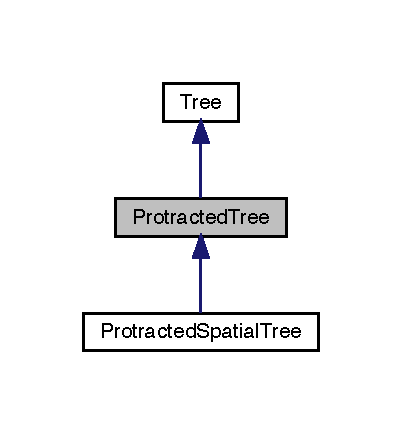
\includegraphics[width=193pt]{class_protracted_tree__inherit__graph}
\end{center}
\end{figure}


Collaboration diagram for Protracted\+Tree\+:\nopagebreak
\begin{figure}[H]
\begin{center}
\leavevmode
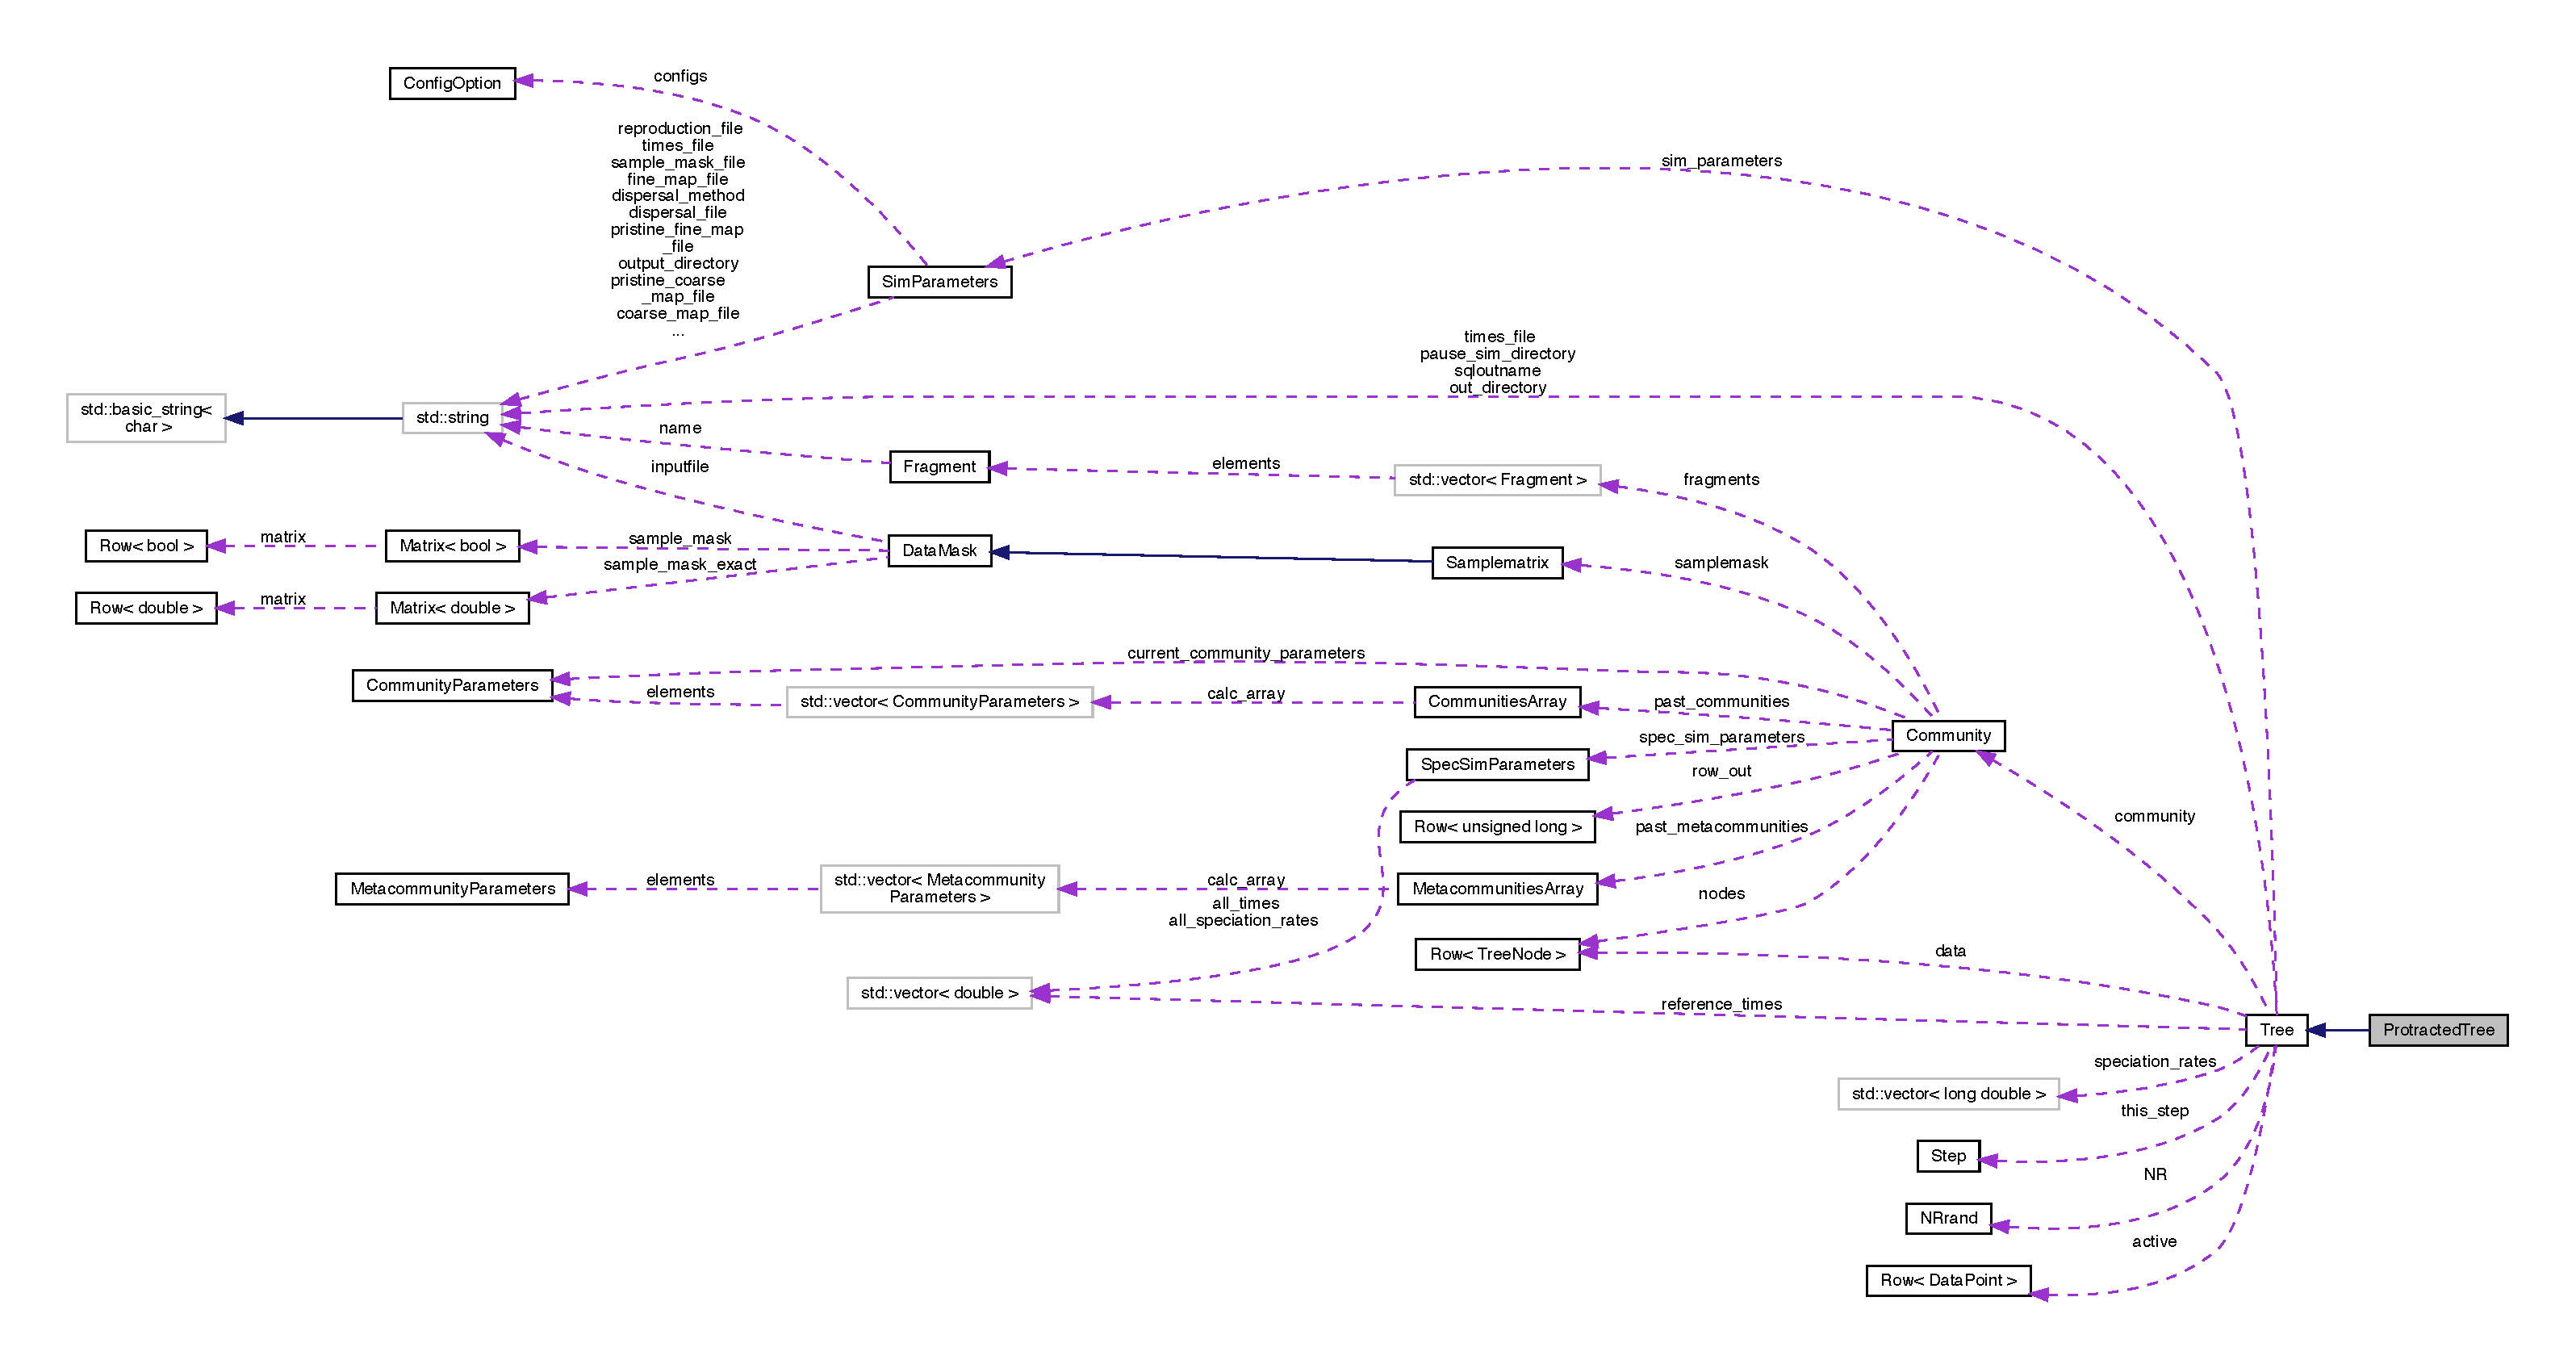
\includegraphics[width=350pt]{class_protracted_tree__coll__graph}
\end{center}
\end{figure}
\subsection*{Public Member Functions}
\begin{DoxyCompactItemize}
\item 
bool \hyperlink{class_protracted_tree_af9690f122e77c0a60d363af3e818c9a2}{calc\+Speciation} (const long double \&random\+\_\+number, const long double \&speciation\+\_\+rate, const unsigned long \&no\+\_\+generations) override
\begin{DoxyCompactList}\small\item\em Calculates the speciation probability from the random number, speciation rate and number of generations a lineage has existed for. \end{DoxyCompactList}\item 
void \hyperlink{class_protracted_tree_aaa2f1db86b0fd49a69d0809bd1c1fb81}{speciate\+Lineage} (const unsigned long \&data\+\_\+position) override
\begin{DoxyCompactList}\small\item\em Performs the actual speciation. Includes handling of speciated lineages under protracted conditions. \end{DoxyCompactList}\item 
bool \hyperlink{class_protracted_tree_ab0bb05fbdeb2aa75a3d3128ded3d655b}{get\+Protracted} () override
\begin{DoxyCompactList}\small\item\em Gets the protractedness of the simulation. Overridden by protracted child classes. \end{DoxyCompactList}\item 
void \hyperlink{class_protracted_tree_a6e04aa92dd30e889a468d9b9fc6fd58d}{set\+Protracted\+Variables} (double speciation\+\_\+gen\+\_\+min, double speciation\+\_\+gen\+\_\+max) override
\begin{DoxyCompactList}\small\item\em Sets the protracted variables. \end{DoxyCompactList}\item 
string \hyperlink{class_protracted_tree_af0eca5eb2a790fcee9a0854e30088753}{get\+Protracted\+Variables} () override
\begin{DoxyCompactList}\small\item\em Gets the protracted variables and returns them as a single, newline separated string. \end{DoxyCompactList}\item 
double \hyperlink{class_protracted_tree_a331561815abc7d595e88d98e9268e7a1}{get\+Protracted\+Generation\+Min} () override
\begin{DoxyCompactList}\small\item\em Gets the minimum number of generations a lineage must exist. \end{DoxyCompactList}\item 
double \hyperlink{class_protracted_tree_a2093dd13cdbfc66e6c1de1406023bad6}{get\+Protracted\+Generation\+Max} () override
\begin{DoxyCompactList}\small\item\em Gets the maximum number of generations a lineage can exist. \end{DoxyCompactList}\item 
string \hyperlink{class_protracted_tree_a505a464578e6a7028e66f26b3e6b4a92}{protracted\+Vars\+To\+String} () override
\begin{DoxyCompactList}\small\item\em Outputs the protracted variables to a string. \end{DoxyCompactList}\item 
void \hyperlink{class_protracted_tree_a56a3631e65bb91d04ba4626c4c1ea79a}{apply\+Spec\+Rate} (double sr, double t)
\begin{DoxyCompactList}\small\item\em Applies the given speciation rate to the tree. \end{DoxyCompactList}\end{DoxyCompactItemize}
\subsection*{Additional Inherited Members}


\subsection{Detailed Description}
\begin{DoxyAuthor}{Author}
Sam Thompson 
\end{DoxyAuthor}
\begin{DoxyDate}{Date}
10/07/2017 
\end{DoxyDate}


\subsection{Member Function Documentation}
\index{Protracted\+Tree@{Protracted\+Tree}!apply\+Spec\+Rate@{apply\+Spec\+Rate}}
\index{apply\+Spec\+Rate@{apply\+Spec\+Rate}!Protracted\+Tree@{Protracted\+Tree}}
\subsubsection[{\texorpdfstring{apply\+Spec\+Rate(double sr, double t)}{applySpecRate(double sr, double t)}}]{\setlength{\rightskip}{0pt plus 5cm}void Protracted\+Tree\+::apply\+Spec\+Rate (
\begin{DoxyParamCaption}
\item[{double}]{sr, }
\item[{double}]{t}
\end{DoxyParamCaption}
)}\hypertarget{class_protracted_tree_a56a3631e65bb91d04ba4626c4c1ea79a}{}\label{class_protracted_tree_a56a3631e65bb91d04ba4626c4c1ea79a}


Applies the given speciation rate to the tree. 

\begin{DoxyNote}{Note}
Currently this just copies code from the version in tree, which is not ideal, but this avoids creating an extra function.
\end{DoxyNote}

\begin{DoxyParams}{Parameters}
{\em sr} & the required speciation rate \\
\hline
\end{DoxyParams}
\index{Protracted\+Tree@{Protracted\+Tree}!calc\+Speciation@{calc\+Speciation}}
\index{calc\+Speciation@{calc\+Speciation}!Protracted\+Tree@{Protracted\+Tree}}
\subsubsection[{\texorpdfstring{calc\+Speciation(const long double \&random\+\_\+number, const long double \&speciation\+\_\+rate, const unsigned long \&no\+\_\+generations) override}{calcSpeciation(const long double &random_number, const long double &speciation_rate, const unsigned long &no_generations) override}}]{\setlength{\rightskip}{0pt plus 5cm}bool Protracted\+Tree\+::calc\+Speciation (
\begin{DoxyParamCaption}
\item[{const long double \&}]{random\+\_\+number, }
\item[{const long double \&}]{speciation\+\_\+rate, }
\item[{const unsigned long \&}]{no\+\_\+generations}
\end{DoxyParamCaption}
)\hspace{0.3cm}{\ttfamily [override]}, {\ttfamily [virtual]}}\hypertarget{class_protracted_tree_af9690f122e77c0a60d363af3e818c9a2}{}\label{class_protracted_tree_af9690f122e77c0a60d363af3e818c9a2}


Calculates the speciation probability from the random number, speciation rate and number of generations a lineage has existed for. 


\begin{DoxyParams}{Parameters}
{\em random\+\_\+number} & the generated random number from 0-\/1 \\
\hline
{\em speciation\+\_\+rate} & the speciation rate to be applied \\
\hline
{\em no\+\_\+generations} & the number of generations a lineage has existed for \\
\hline
\end{DoxyParams}
\begin{DoxyReturn}{Returns}
if true, speciation has occured 
\end{DoxyReturn}


Reimplemented from \hyperlink{class_tree_abc9389511e1aecf5e573315fc8f4d77c}{Tree}.

\index{Protracted\+Tree@{Protracted\+Tree}!get\+Protracted@{get\+Protracted}}
\index{get\+Protracted@{get\+Protracted}!Protracted\+Tree@{Protracted\+Tree}}
\subsubsection[{\texorpdfstring{get\+Protracted() override}{getProtracted() override}}]{\setlength{\rightskip}{0pt plus 5cm}bool Protracted\+Tree\+::get\+Protracted (
\begin{DoxyParamCaption}
{}
\end{DoxyParamCaption}
)\hspace{0.3cm}{\ttfamily [override]}, {\ttfamily [virtual]}}\hypertarget{class_protracted_tree_ab0bb05fbdeb2aa75a3d3128ded3d655b}{}\label{class_protracted_tree_ab0bb05fbdeb2aa75a3d3128ded3d655b}


Gets the protractedness of the simulation. Overridden by protracted child classes. 

\begin{DoxyReturn}{Returns}

\end{DoxyReturn}


Reimplemented from \hyperlink{class_tree_aa23a57f7863d58384f61d464d998ab3c}{Tree}.

\index{Protracted\+Tree@{Protracted\+Tree}!get\+Protracted\+Generation\+Max@{get\+Protracted\+Generation\+Max}}
\index{get\+Protracted\+Generation\+Max@{get\+Protracted\+Generation\+Max}!Protracted\+Tree@{Protracted\+Tree}}
\subsubsection[{\texorpdfstring{get\+Protracted\+Generation\+Max() override}{getProtractedGenerationMax() override}}]{\setlength{\rightskip}{0pt plus 5cm}double Protracted\+Tree\+::get\+Protracted\+Generation\+Max (
\begin{DoxyParamCaption}
{}
\end{DoxyParamCaption}
)\hspace{0.3cm}{\ttfamily [override]}, {\ttfamily [virtual]}}\hypertarget{class_protracted_tree_a2093dd13cdbfc66e6c1de1406023bad6}{}\label{class_protracted_tree_a2093dd13cdbfc66e6c1de1406023bad6}


Gets the maximum number of generations a lineage can exist. 

\begin{DoxyReturn}{Returns}
double the number of generations a lineage must exist 
\end{DoxyReturn}


Reimplemented from \hyperlink{class_tree_a0c5e746982a87f24c083f4534bf92b45}{Tree}.

\index{Protracted\+Tree@{Protracted\+Tree}!get\+Protracted\+Generation\+Min@{get\+Protracted\+Generation\+Min}}
\index{get\+Protracted\+Generation\+Min@{get\+Protracted\+Generation\+Min}!Protracted\+Tree@{Protracted\+Tree}}
\subsubsection[{\texorpdfstring{get\+Protracted\+Generation\+Min() override}{getProtractedGenerationMin() override}}]{\setlength{\rightskip}{0pt plus 5cm}double Protracted\+Tree\+::get\+Protracted\+Generation\+Min (
\begin{DoxyParamCaption}
{}
\end{DoxyParamCaption}
)\hspace{0.3cm}{\ttfamily [override]}, {\ttfamily [virtual]}}\hypertarget{class_protracted_tree_a331561815abc7d595e88d98e9268e7a1}{}\label{class_protracted_tree_a331561815abc7d595e88d98e9268e7a1}


Gets the minimum number of generations a lineage must exist. 

\begin{DoxyReturn}{Returns}
double the number of generations a lineage must exist 
\end{DoxyReturn}


Reimplemented from \hyperlink{class_tree_a6ffc42e941f352cd74f01f6f7011f00b}{Tree}.

\index{Protracted\+Tree@{Protracted\+Tree}!get\+Protracted\+Variables@{get\+Protracted\+Variables}}
\index{get\+Protracted\+Variables@{get\+Protracted\+Variables}!Protracted\+Tree@{Protracted\+Tree}}
\subsubsection[{\texorpdfstring{get\+Protracted\+Variables() override}{getProtractedVariables() override}}]{\setlength{\rightskip}{0pt plus 5cm}string Protracted\+Tree\+::get\+Protracted\+Variables (
\begin{DoxyParamCaption}
{}
\end{DoxyParamCaption}
)\hspace{0.3cm}{\ttfamily [override]}, {\ttfamily [virtual]}}\hypertarget{class_protracted_tree_af0eca5eb2a790fcee9a0854e30088753}{}\label{class_protracted_tree_af0eca5eb2a790fcee9a0854e30088753}


Gets the protracted variables and returns them as a single, newline separated string. 

\begin{DoxyReturn}{Returns}
string containing the protracted variables, separated by newlines. 
\end{DoxyReturn}


Reimplemented from \hyperlink{class_tree_a34c0808026bf00546c8f9786376be730}{Tree}.

\index{Protracted\+Tree@{Protracted\+Tree}!protracted\+Vars\+To\+String@{protracted\+Vars\+To\+String}}
\index{protracted\+Vars\+To\+String@{protracted\+Vars\+To\+String}!Protracted\+Tree@{Protracted\+Tree}}
\subsubsection[{\texorpdfstring{protracted\+Vars\+To\+String() override}{protractedVarsToString() override}}]{\setlength{\rightskip}{0pt plus 5cm}string Protracted\+Tree\+::protracted\+Vars\+To\+String (
\begin{DoxyParamCaption}
{}
\end{DoxyParamCaption}
)\hspace{0.3cm}{\ttfamily [override]}, {\ttfamily [virtual]}}\hypertarget{class_protracted_tree_a505a464578e6a7028e66f26b3e6b4a92}{}\label{class_protracted_tree_a505a464578e6a7028e66f26b3e6b4a92}


Outputs the protracted variables to a string. 

This function is intended to be overridden by derived classes. It is intended the output is used for writing to S\+QL databases.

\begin{DoxyReturn}{Returns}
string containing a list of the protracted speciation variables. 
\end{DoxyReturn}


Reimplemented from \hyperlink{class_tree_aa8bb5d93c7992404ede0a49bb69ccd1f}{Tree}.

\index{Protracted\+Tree@{Protracted\+Tree}!set\+Protracted\+Variables@{set\+Protracted\+Variables}}
\index{set\+Protracted\+Variables@{set\+Protracted\+Variables}!Protracted\+Tree@{Protracted\+Tree}}
\subsubsection[{\texorpdfstring{set\+Protracted\+Variables(double speciation\+\_\+gen\+\_\+min, double speciation\+\_\+gen\+\_\+max) override}{setProtractedVariables(double speciation_gen_min, double speciation_gen_max) override}}]{\setlength{\rightskip}{0pt plus 5cm}void Protracted\+Tree\+::set\+Protracted\+Variables (
\begin{DoxyParamCaption}
\item[{double}]{speciation\+\_\+gen\+\_\+min, }
\item[{double}]{speciation\+\_\+gen\+\_\+max}
\end{DoxyParamCaption}
)\hspace{0.3cm}{\ttfamily [override]}, {\ttfamily [virtual]}}\hypertarget{class_protracted_tree_a6e04aa92dd30e889a468d9b9fc6fd58d}{}\label{class_protracted_tree_a6e04aa92dd30e889a468d9b9fc6fd58d}


Sets the protracted variables. 


\begin{DoxyParams}{Parameters}
{\em speciation\+\_\+gen\+\_\+min} & the minimum number of generations to have passed before speciation is allowed \\
\hline
{\em speciation\+\_\+gen\+\_\+max} & the maximum number of generations a lineage can exist for before it is speciated. \\
\hline
\end{DoxyParams}


Reimplemented from \hyperlink{class_tree_a891764ffc1e29d3edbe0fd08e67a184b}{Tree}.

\index{Protracted\+Tree@{Protracted\+Tree}!speciate\+Lineage@{speciate\+Lineage}}
\index{speciate\+Lineage@{speciate\+Lineage}!Protracted\+Tree@{Protracted\+Tree}}
\subsubsection[{\texorpdfstring{speciate\+Lineage(const unsigned long \&data\+\_\+position) override}{speciateLineage(const unsigned long &data_position) override}}]{\setlength{\rightskip}{0pt plus 5cm}void Protracted\+Tree\+::speciate\+Lineage (
\begin{DoxyParamCaption}
\item[{const unsigned long \&}]{data\+\_\+position}
\end{DoxyParamCaption}
)\hspace{0.3cm}{\ttfamily [override]}, {\ttfamily [virtual]}}\hypertarget{class_protracted_tree_aaa2f1db86b0fd49a69d0809bd1c1fb81}{}\label{class_protracted_tree_aaa2f1db86b0fd49a69d0809bd1c1fb81}


Performs the actual speciation. Includes handling of speciated lineages under protracted conditions. 


\begin{DoxyParams}{Parameters}
{\em data\+\_\+position} & the position in the array of Tree\+Nodes for this lineage \\
\hline
\end{DoxyParams}


Reimplemented from \hyperlink{class_tree_a32e12cc62ce2d9ae893214b1f4cfad1f}{Tree}.



The documentation for this class was generated from the following files\+:\begin{DoxyCompactItemize}
\item 
necsim/\hyperlink{_protracted_tree_8h}{Protracted\+Tree.\+h}\item 
necsim/\hyperlink{_protracted_tree_8cpp}{Protracted\+Tree.\+cpp}\end{DoxyCompactItemize}

\hypertarget{class_reproduction_map}{}\section{Reproduction\+Map Class Reference}
\label{class_reproduction_map}\index{Reproduction\+Map@{Reproduction\+Map}}


Contains the routines for importing the reproduction map and getting a cell value from the map.  




{\ttfamily \#include $<$Reproduction\+Map.\+h$>$}



Collaboration diagram for Reproduction\+Map\+:
% FIG 0
\subsection*{Public Member Functions}
\begin{DoxyCompactItemize}
\item 
void \hyperlink{class_reproduction_map_a144d2f39ff2e978acd9d2ebcb6f8dc97}{import} (string file\+\_\+name, unsigned long size\+\_\+x, unsigned long size\+\_\+y)
\begin{DoxyCompactList}\small\item\em Imports the map file from the given path Requires the dimensions to be identical as the fine map file dimensions. \end{DoxyCompactList}\item 
void \hyperlink{class_reproduction_map_afc0419bc78ce9a4813212360c67b49a2}{set\+Reproduction\+Function} ()\hypertarget{class_reproduction_map_afc0419bc78ce9a4813212360c67b49a2}{}\label{class_reproduction_map_afc0419bc78ce9a4813212360c67b49a2}

\begin{DoxyCompactList}\small\item\em Correctly sets the reproduction function to either rejection\+Sample\+Null or rejection\+Sample depending on if a reproduction map is used or not. \end{DoxyCompactList}\item 
void \hyperlink{class_reproduction_map_aba75d30a9d2c7cd8aa06db17af286f7d}{set\+Offsets} (const unsigned long \&x\+\_\+offset, const unsigned long \&y\+\_\+offset, const unsigned long \&xdim, const unsigned long \&ydim)
\begin{DoxyCompactList}\small\item\em Sets the offsets for the reproduction map from the sample grid. \end{DoxyCompactList}\item 
bool \hyperlink{class_reproduction_map_a80dfa3194b7acabd813d9ae6b4ae3671}{rejection\+Sample\+Null} (\hyperlink{class_n_rrand}{N\+Rrand} \&random\+\_\+number, const unsigned long \&x, const unsigned long \&y, const long \&xwrap, const long \&ywrap)
\begin{DoxyCompactList}\small\item\em Returns true for all cell values Function to be pointed to in cases where there is no reproduction map. \end{DoxyCompactList}\item 
bool \hyperlink{class_reproduction_map_a2dccd14c9d4cdc1b14a63e7d95eba0ae}{rejection\+Sample} (\hyperlink{class_n_rrand}{N\+Rrand} \&random\+\_\+number, const unsigned long \&x, const unsigned long \&y, const long \&xwrap, const long \&ywrap)
\begin{DoxyCompactList}\small\item\em Returns true for all cell values Function to be pointed to in cases where there is no reproduction map. \end{DoxyCompactList}\item 
double \hyperlink{class_reproduction_map_a36cb74792a8e935eec6f7fcb6af3aeb8}{get\+Val} (const unsigned long \&x, const unsigned long \&y, const long \&xwrap, const long \&ywrap)
\begin{DoxyCompactList}\small\item\em Gets the value of the reproduction map at that location. \end{DoxyCompactList}\item 
bool \hyperlink{class_reproduction_map_aa8afbdf28197532a65c17035a075fe9b}{has\+Reproduced} (\hyperlink{class_n_rrand}{N\+Rrand} \&random\+\_\+number, const unsigned long \&x, const unsigned long \&y, const long \&xwrap, const long \&ywrap)
\item 
\hyperlink{class_row}{Row}$<$ double $>$ \hyperlink{class_reproduction_map_ad9489c17cf27be65c21f54ff20e6ccc8}{operator\mbox{[}$\,$\mbox{]}} (long index)
\begin{DoxyCompactList}\small\item\em Operator \mbox{[}\mbox{]} for getting values directly from the reproduction map. \end{DoxyCompactList}\end{DoxyCompactItemize}
\subsection*{Protected Types}
\begin{DoxyCompactItemize}
\item 
typedef bool(Reproduction\+Map\+::$\ast$ {\bfseries rep\+\_\+ptr}) (\hyperlink{class_n_rrand}{N\+Rrand} \&random\+\_\+no, const unsigned long \&x, const unsigned long \&y, const long \&xwrap, const long \&ywrap)\hypertarget{class_reproduction_map_a5edd07fa5fe2f2ecbd778f2fa20d2a88}{}\label{class_reproduction_map_a5edd07fa5fe2f2ecbd778f2fa20d2a88}

\end{DoxyCompactItemize}
\subsection*{Protected Attributes}
\begin{DoxyCompactItemize}
\item 
\hyperlink{class_matrix}{Matrix}$<$ double $>$ {\bfseries reproduction\+\_\+map}\hypertarget{class_reproduction_map_a4092819111e3b20c8c6bbd189a81def7}{}\label{class_reproduction_map_a4092819111e3b20c8c6bbd189a81def7}

\item 
string {\bfseries map\+\_\+file}\hypertarget{class_reproduction_map_a4fdefab63d92f1244422b602ef11b2ee}{}\label{class_reproduction_map_a4fdefab63d92f1244422b602ef11b2ee}

\item 
double {\bfseries max\+\_\+val}\hypertarget{class_reproduction_map_a093ebaad740e4d8b0873bb6e96e5e1c1}{}\label{class_reproduction_map_a093ebaad740e4d8b0873bb6e96e5e1c1}

\item 
bool {\bfseries null\+\_\+map}\hypertarget{class_reproduction_map_a3ae593187d7087cb543f40fe59218257}{}\label{class_reproduction_map_a3ae593187d7087cb543f40fe59218257}

\item 
unsigned long {\bfseries offset\+\_\+x}\hypertarget{class_reproduction_map_acaa2a99d3667440a1e610fd1d0ecda7e}{}\label{class_reproduction_map_acaa2a99d3667440a1e610fd1d0ecda7e}

\item 
unsigned long {\bfseries offset\+\_\+y}\hypertarget{class_reproduction_map_ae70ca7adb1272ed2a15287108526351b}{}\label{class_reproduction_map_ae70ca7adb1272ed2a15287108526351b}

\item 
unsigned long {\bfseries x\+\_\+dim}\hypertarget{class_reproduction_map_aea934c598f314851c50a9d5aa12f8035}{}\label{class_reproduction_map_aea934c598f314851c50a9d5aa12f8035}

\item 
unsigned long {\bfseries y\+\_\+dim}\hypertarget{class_reproduction_map_a48dcb8efff54b3734d2a560f6660dc18}{}\label{class_reproduction_map_a48dcb8efff54b3734d2a560f6660dc18}

\item 
rep\+\_\+ptr {\bfseries reproduction\+Map\+Checker\+\_\+fptr}\hypertarget{class_reproduction_map_a927b35c48a2c3c32a994a95ebfb9aa87}{}\label{class_reproduction_map_a927b35c48a2c3c32a994a95ebfb9aa87}

\end{DoxyCompactItemize}
\subsection*{Friends}
\begin{DoxyCompactItemize}
\item 
ostream \& \hyperlink{class_reproduction_map_a98af33155ec460fb9b9c55fa53458262}{operator$<$$<$} (ostream \&os, \hyperlink{class_reproduction_map}{Reproduction\+Map} \&r)
\begin{DoxyCompactList}\small\item\em Operator for outputting to an ostream. \end{DoxyCompactList}\item 
istream \& \hyperlink{class_reproduction_map_a7cffbc069ece5bfb93d296580e22892a}{operator$>$$>$} (istream \&is, \hyperlink{class_reproduction_map}{Reproduction\+Map} \&r)
\begin{DoxyCompactList}\small\item\em Operator for inputting from an istream. \end{DoxyCompactList}\end{DoxyCompactItemize}


\subsection{Detailed Description}
Contains the routines for importing the reproduction map and getting a cell value from the map. 

\subsection{Member Function Documentation}
\index{Reproduction\+Map@{Reproduction\+Map}!get\+Val@{get\+Val}}
\index{get\+Val@{get\+Val}!Reproduction\+Map@{Reproduction\+Map}}
\subsubsection[{\texorpdfstring{get\+Val(const unsigned long \&x, const unsigned long \&y, const long \&xwrap, const long \&ywrap)}{getVal(const unsigned long &x, const unsigned long &y, const long &xwrap, const long &ywrap)}}]{\setlength{\rightskip}{0pt plus 5cm}double Reproduction\+Map\+::get\+Val (
\begin{DoxyParamCaption}
\item[{const unsigned long \&}]{x, }
\item[{const unsigned long \&}]{y, }
\item[{const long \&}]{xwrap, }
\item[{const long \&}]{ywrap}
\end{DoxyParamCaption}
)}\hypertarget{class_reproduction_map_a36cb74792a8e935eec6f7fcb6af3aeb8}{}\label{class_reproduction_map_a36cb74792a8e935eec6f7fcb6af3aeb8}


Gets the value of the reproduction map at that location. 


\begin{DoxyParams}{Parameters}
{\em x} & x coordinate of the lineage on the sample grid \\
\hline
{\em y} & y coordinate of the lineage on the sample grid \\
\hline
{\em xwrap} & x wrapping of the lineage \\
\hline
{\em ywrap} & y wrapping of the lineage \\
\hline
\end{DoxyParams}
\begin{DoxyReturn}{Returns}
value of the reproduction map at the required location 
\end{DoxyReturn}
\index{Reproduction\+Map@{Reproduction\+Map}!has\+Reproduced@{has\+Reproduced}}
\index{has\+Reproduced@{has\+Reproduced}!Reproduction\+Map@{Reproduction\+Map}}
\subsubsection[{\texorpdfstring{has\+Reproduced(\+N\+Rrand \&random\+\_\+number, const unsigned long \&x, const unsigned long \&y, const long \&xwrap, const long \&ywrap)}{hasReproduced(NRrand &random_number, const unsigned long &x, const unsigned long &y, const long &xwrap, const long &ywrap)}}]{\setlength{\rightskip}{0pt plus 5cm}bool Reproduction\+Map\+::has\+Reproduced (
\begin{DoxyParamCaption}
\item[{{\bf N\+Rrand} \&}]{random\+\_\+number, }
\item[{const unsigned long \&}]{x, }
\item[{const unsigned long \&}]{y, }
\item[{const long \&}]{xwrap, }
\item[{const long \&}]{ywrap}
\end{DoxyParamCaption}
)}\hypertarget{class_reproduction_map_aa8afbdf28197532a65c17035a075fe9b}{}\label{class_reproduction_map_aa8afbdf28197532a65c17035a075fe9b}

\begin{DoxyParams}{Parameters}
{\em random\+\_\+number} & random number object to draw from \\
\hline
{\em x} & x coordinate of the lineage on the sample grid \\
\hline
{\em y} & y coordinate of the lineage on the sample grid \\
\hline
{\em xwrap} & x wrapping of the lineage \\
\hline
{\em ywrap} & y wrapping of the lineage \\
\hline
\end{DoxyParams}
\begin{DoxyReturn}{Returns}
value of the reproduction map at the required location 
\end{DoxyReturn}
\index{Reproduction\+Map@{Reproduction\+Map}!import@{import}}
\index{import@{import}!Reproduction\+Map@{Reproduction\+Map}}
\subsubsection[{\texorpdfstring{import(string file\+\_\+name, unsigned long size\+\_\+x, unsigned long size\+\_\+y)}{import(string file_name, unsigned long size_x, unsigned long size_y)}}]{\setlength{\rightskip}{0pt plus 5cm}void Reproduction\+Map\+::import (
\begin{DoxyParamCaption}
\item[{string}]{file\+\_\+name, }
\item[{unsigned long}]{size\+\_\+x, }
\item[{unsigned long}]{size\+\_\+y}
\end{DoxyParamCaption}
)}\hypertarget{class_reproduction_map_a144d2f39ff2e978acd9d2ebcb6f8dc97}{}\label{class_reproduction_map_a144d2f39ff2e978acd9d2ebcb6f8dc97}


Imports the map file from the given path Requires the dimensions to be identical as the fine map file dimensions. 


\begin{DoxyParams}{Parameters}
{\em file\+\_\+name} & the path to the reproduction map to import \\
\hline
{\em size\+\_\+x} & the x dimensions of the map file \\
\hline
{\em size\+\_\+y} & the y dimensions of the map file \\
\hline
\end{DoxyParams}
\index{Reproduction\+Map@{Reproduction\+Map}!operator\mbox{[}$\,$\mbox{]}@{operator[]}}
\index{operator\mbox{[}$\,$\mbox{]}@{operator[]}!Reproduction\+Map@{Reproduction\+Map}}
\subsubsection[{\texorpdfstring{operator[](long index)}{operator[](long index)}}]{\setlength{\rightskip}{0pt plus 5cm}{\bf Row}$<$double$>$ Reproduction\+Map\+::operator\mbox{[}$\,$\mbox{]} (
\begin{DoxyParamCaption}
\item[{long}]{index}
\end{DoxyParamCaption}
)\hspace{0.3cm}{\ttfamily [inline]}}\hypertarget{class_reproduction_map_ad9489c17cf27be65c21f54ff20e6ccc8}{}\label{class_reproduction_map_ad9489c17cf27be65c21f54ff20e6ccc8}


Operator \mbox{[}\mbox{]} for getting values directly from the reproduction map. 


\begin{DoxyParams}{Parameters}
{\em index} & the index to get the row of \\
\hline
\end{DoxyParams}
\begin{DoxyReturn}{Returns}
the row present at that index 
\end{DoxyReturn}
\index{Reproduction\+Map@{Reproduction\+Map}!rejection\+Sample@{rejection\+Sample}}
\index{rejection\+Sample@{rejection\+Sample}!Reproduction\+Map@{Reproduction\+Map}}
\subsubsection[{\texorpdfstring{rejection\+Sample(\+N\+Rrand \&random\+\_\+number, const unsigned long \&x, const unsigned long \&y, const long \&xwrap, const long \&ywrap)}{rejectionSample(NRrand &random_number, const unsigned long &x, const unsigned long &y, const long &xwrap, const long &ywrap)}}]{\setlength{\rightskip}{0pt plus 5cm}bool Reproduction\+Map\+::rejection\+Sample (
\begin{DoxyParamCaption}
\item[{{\bf N\+Rrand} \&}]{random\+\_\+number, }
\item[{const unsigned long \&}]{x, }
\item[{const unsigned long \&}]{y, }
\item[{const long \&}]{xwrap, }
\item[{const long \&}]{ywrap}
\end{DoxyParamCaption}
)}\hypertarget{class_reproduction_map_a2dccd14c9d4cdc1b14a63e7d95eba0ae}{}\label{class_reproduction_map_a2dccd14c9d4cdc1b14a63e7d95eba0ae}


Returns true for all cell values Function to be pointed to in cases where there is no reproduction map. 


\begin{DoxyParams}{Parameters}
{\em random\+\_\+number} & random number object to pass forward \\
\hline
{\em x} & x coordinate of the lineage on the sample grid \\
\hline
{\em y} & y coordinate of the lineage on the sample grid \\
\hline
{\em xwrap} & x wrapping of the lineage \\
\hline
{\em ywrap} & y wrapping of the lineage \\
\hline
\end{DoxyParams}
\begin{DoxyReturn}{Returns}
true always 
\end{DoxyReturn}
\index{Reproduction\+Map@{Reproduction\+Map}!rejection\+Sample\+Null@{rejection\+Sample\+Null}}
\index{rejection\+Sample\+Null@{rejection\+Sample\+Null}!Reproduction\+Map@{Reproduction\+Map}}
\subsubsection[{\texorpdfstring{rejection\+Sample\+Null(\+N\+Rrand \&random\+\_\+number, const unsigned long \&x, const unsigned long \&y, const long \&xwrap, const long \&ywrap)}{rejectionSampleNull(NRrand &random_number, const unsigned long &x, const unsigned long &y, const long &xwrap, const long &ywrap)}}]{\setlength{\rightskip}{0pt plus 5cm}bool Reproduction\+Map\+::rejection\+Sample\+Null (
\begin{DoxyParamCaption}
\item[{{\bf N\+Rrand} \&}]{random\+\_\+number, }
\item[{const unsigned long \&}]{x, }
\item[{const unsigned long \&}]{y, }
\item[{const long \&}]{xwrap, }
\item[{const long \&}]{ywrap}
\end{DoxyParamCaption}
)}\hypertarget{class_reproduction_map_a80dfa3194b7acabd813d9ae6b4ae3671}{}\label{class_reproduction_map_a80dfa3194b7acabd813d9ae6b4ae3671}


Returns true for all cell values Function to be pointed to in cases where there is no reproduction map. 


\begin{DoxyParams}{Parameters}
{\em random\+\_\+number} & random number object to pass forward \\
\hline
{\em x} & x coordinate of the lineage on the sample grid \\
\hline
{\em y} & y coordinate of the lineage on the sample grid \\
\hline
{\em xwrap} & x wrapping of the lineage \\
\hline
{\em ywrap} & y wrapping of the lineage \\
\hline
\end{DoxyParams}
\begin{DoxyReturn}{Returns}
true always 
\end{DoxyReturn}
\index{Reproduction\+Map@{Reproduction\+Map}!set\+Offsets@{set\+Offsets}}
\index{set\+Offsets@{set\+Offsets}!Reproduction\+Map@{Reproduction\+Map}}
\subsubsection[{\texorpdfstring{set\+Offsets(const unsigned long \&x\+\_\+offset, const unsigned long \&y\+\_\+offset, const unsigned long \&xdim, const unsigned long \&ydim)}{setOffsets(const unsigned long &x_offset, const unsigned long &y_offset, const unsigned long &xdim, const unsigned long &ydim)}}]{\setlength{\rightskip}{0pt plus 5cm}void Reproduction\+Map\+::set\+Offsets (
\begin{DoxyParamCaption}
\item[{const unsigned long \&}]{x\+\_\+offset, }
\item[{const unsigned long \&}]{y\+\_\+offset, }
\item[{const unsigned long \&}]{xdim, }
\item[{const unsigned long \&}]{ydim}
\end{DoxyParamCaption}
)}\hypertarget{class_reproduction_map_aba75d30a9d2c7cd8aa06db17af286f7d}{}\label{class_reproduction_map_aba75d30a9d2c7cd8aa06db17af286f7d}


Sets the offsets for the reproduction map from the sample grid. 


\begin{DoxyParams}{Parameters}
{\em x\+\_\+offset} & the x offset from the sample grid \\
\hline
{\em y\+\_\+offset} & the y offset from the sample grid \\
\hline
{\em xdim} & the x dimension of the sample grid \\
\hline
{\em ydim} & the y dimension of the sample grid \\
\hline
\end{DoxyParams}


\subsection{Friends And Related Function Documentation}
\index{Reproduction\+Map@{Reproduction\+Map}!operator$<$$<$@{operator$<$$<$}}
\index{operator$<$$<$@{operator$<$$<$}!Reproduction\+Map@{Reproduction\+Map}}
\subsubsection[{\texorpdfstring{operator$<$$<$}{operator<<}}]{\setlength{\rightskip}{0pt plus 5cm}ostream\& operator$<$$<$ (
\begin{DoxyParamCaption}
\item[{ostream \&}]{os, }
\item[{{\bf Reproduction\+Map} \&}]{r}
\end{DoxyParamCaption}
)\hspace{0.3cm}{\ttfamily [friend]}}\hypertarget{class_reproduction_map_a98af33155ec460fb9b9c55fa53458262}{}\label{class_reproduction_map_a98af33155ec460fb9b9c55fa53458262}


Operator for outputting to an ostream. 


\begin{DoxyParams}{Parameters}
{\em os} & the ostream to output to \\
\hline
{\em r} & the \hyperlink{class_reproduction_map}{Reproduction\+Map} to read from \\
\hline
\end{DoxyParams}
\begin{DoxyReturn}{Returns}
the os object 
\end{DoxyReturn}
\index{Reproduction\+Map@{Reproduction\+Map}!operator$>$$>$@{operator$>$$>$}}
\index{operator$>$$>$@{operator$>$$>$}!Reproduction\+Map@{Reproduction\+Map}}
\subsubsection[{\texorpdfstring{operator$>$$>$}{operator>>}}]{\setlength{\rightskip}{0pt plus 5cm}istream\& operator$>$$>$ (
\begin{DoxyParamCaption}
\item[{istream \&}]{is, }
\item[{{\bf Reproduction\+Map} \&}]{r}
\end{DoxyParamCaption}
)\hspace{0.3cm}{\ttfamily [friend]}}\hypertarget{class_reproduction_map_a7cffbc069ece5bfb93d296580e22892a}{}\label{class_reproduction_map_a7cffbc069ece5bfb93d296580e22892a}


Operator for inputting from an istream. 


\begin{DoxyParams}{Parameters}
{\em is} & the istream to input from \\
\hline
{\em r} & the \hyperlink{class_reproduction_map}{Reproduction\+Map} to input to \\
\hline
\end{DoxyParams}
\begin{DoxyReturn}{Returns}
the is object 
\end{DoxyReturn}


The documentation for this class was generated from the following files\+:\begin{DoxyCompactItemize}
\item 
\hyperlink{_reproduction_map_8h}{Reproduction\+Map.\+h}\item 
\hyperlink{_reproduction_map_8cpp}{Reproduction\+Map.\+cpp}\end{DoxyCompactItemize}

\hypertarget{class_row}{}\section{Row$<$ T $>$ Class Template Reference}
\label{class_row}\index{Row$<$ T $>$@{Row$<$ T $>$}}


Contains a template \hyperlink{class_row}{Row} class and basic operations. Uses an array to store the row.  




{\ttfamily \#include $<$Matrix.\+h$>$}

\subsection*{Public Member Functions}
\begin{DoxyCompactItemize}
\item 
\hyperlink{class_row_a32774cba0d7cdb6f0d7100c395ece9e5}{Row} (unsigned long cols=0)
\begin{DoxyCompactList}\small\item\em Standard constructor. \end{DoxyCompactList}\item 
\hyperlink{class_row_a8e888a33060156cd2e3757a95e9feee1}{$\sim$\+Row} ()\hypertarget{class_row_a8e888a33060156cd2e3757a95e9feee1}{}\label{class_row_a8e888a33060156cd2e3757a95e9feee1}

\begin{DoxyCompactList}\small\item\em Standard destructor. \end{DoxyCompactList}\item 
\hyperlink{class_row_a3c76905ddd4522c92da0d8a9e24a22a1}{Row} (const \hyperlink{class_row}{Row} \&r)
\begin{DoxyCompactList}\small\item\em Copy constructor. \end{DoxyCompactList}\item 
void \hyperlink{class_row_a4015d3cc7a22a4a4ad31ae410ab8fce4}{set\+Size} (unsigned long n)
\begin{DoxyCompactList}\small\item\em Setter for the row size. \end{DoxyCompactList}\item 
void \hyperlink{class_row_aac3e65388e6ce2a003be1a1b460fab53}{resize} (unsigned long n)
\begin{DoxyCompactList}\small\item\em Changes the size of the array. \end{DoxyCompactList}\item 
unsigned long \hyperlink{class_row_a5fdbcb2478b0ff00d12b8b109b0eb89a}{size} ()
\begin{DoxyCompactList}\small\item\em Getter for the size of the array. \end{DoxyCompactList}\item 
T \& \hyperlink{class_row_aecb642c8ceffbb7d6c69bc13d9de4bb0}{operator\mbox{[}$\,$\mbox{]}} (unsigned long column)
\begin{DoxyCompactList}\small\item\em Overloading the \mbox{[}\mbox{]} operator to allow for simple referencing. \end{DoxyCompactList}\item 
\hyperlink{class_row}{Row} \& \hyperlink{class_row_a877484e061eef2a179cc28d30b3ec542}{operator=} (const \hyperlink{class_row}{Row} \&r)
\begin{DoxyCompactList}\small\item\em Overloading the = operator to allow for copying data across. \end{DoxyCompactList}\end{DoxyCompactItemize}
\subsection*{Friends}
\begin{DoxyCompactItemize}
\item 
ostream \& \hyperlink{class_row_a8aaaee73ace04bfd4dda937bc311a16e}{operator$<$$<$} (ostream \&os, const \hyperlink{class_row}{Row} \&r)
\begin{DoxyCompactList}\small\item\em Overloading the $<$$<$ operator for outputting to the output stream. \end{DoxyCompactList}\item 
istream \& \hyperlink{class_row_adaa9bd295e9b13a99d9205911763468c}{operator$>$$>$} (istream \&is, \hyperlink{class_row}{Row} \&r)
\begin{DoxyCompactList}\small\item\em Overloading the $<$$<$ operator for inputting from an input stream. \end{DoxyCompactList}\end{DoxyCompactItemize}


\subsection{Detailed Description}
\subsubsection*{template$<$class T$>$\\*
class Row$<$ T $>$}

Contains a template \hyperlink{class_row}{Row} class and basic operations. Uses an array to store the row. 

\subsection{Constructor \& Destructor Documentation}
\index{Row@{Row}!Row@{Row}}
\index{Row@{Row}!Row@{Row}}
\subsubsection[{\texorpdfstring{Row(unsigned long cols=0)}{Row(unsigned long cols=0)}}]{\setlength{\rightskip}{0pt plus 5cm}template$<$class T$>$ {\bf Row}$<$ T $>$\+::{\bf Row} (
\begin{DoxyParamCaption}
\item[{unsigned long}]{cols = {\ttfamily 0}}
\end{DoxyParamCaption}
)\hspace{0.3cm}{\ttfamily [inline]}, {\ttfamily [explicit]}}\hypertarget{class_row_a32774cba0d7cdb6f0d7100c395ece9e5}{}\label{class_row_a32774cba0d7cdb6f0d7100c395ece9e5}


Standard constructor. 


\begin{DoxyParams}{Parameters}
{\em cols} & optionally provide the number of rows to initiate with. \\
\hline
\end{DoxyParams}
\index{Row@{Row}!Row@{Row}}
\index{Row@{Row}!Row@{Row}}
\subsubsection[{\texorpdfstring{Row(const Row \&r)}{Row(const Row &r)}}]{\setlength{\rightskip}{0pt plus 5cm}template$<$class T$>$ {\bf Row}$<$ T $>$\+::{\bf Row} (
\begin{DoxyParamCaption}
\item[{const {\bf Row}$<$ T $>$ \&}]{r}
\end{DoxyParamCaption}
)\hspace{0.3cm}{\ttfamily [inline]}}\hypertarget{class_row_a3c76905ddd4522c92da0d8a9e24a22a1}{}\label{class_row_a3c76905ddd4522c92da0d8a9e24a22a1}


Copy constructor. 


\begin{DoxyParams}{Parameters}
{\em r} & the \hyperlink{class_row}{Row} object to copy from. \\
\hline
\end{DoxyParams}


\subsection{Member Function Documentation}
\index{Row@{Row}!operator=@{operator=}}
\index{operator=@{operator=}!Row@{Row}}
\subsubsection[{\texorpdfstring{operator=(const Row \&r)}{operator=(const Row &r)}}]{\setlength{\rightskip}{0pt plus 5cm}template$<$class T$>$ {\bf Row}\& {\bf Row}$<$ T $>$\+::operator= (
\begin{DoxyParamCaption}
\item[{const {\bf Row}$<$ T $>$ \&}]{r}
\end{DoxyParamCaption}
)\hspace{0.3cm}{\ttfamily [inline]}}\hypertarget{class_row_a877484e061eef2a179cc28d30b3ec542}{}\label{class_row_a877484e061eef2a179cc28d30b3ec542}


Overloading the = operator to allow for copying data across. 


\begin{DoxyParams}{Parameters}
{\em r} & the \hyperlink{class_row}{Row} object to copy data from. \\
\hline
\end{DoxyParams}
\index{Row@{Row}!operator\mbox{[}$\,$\mbox{]}@{operator[]}}
\index{operator\mbox{[}$\,$\mbox{]}@{operator[]}!Row@{Row}}
\subsubsection[{\texorpdfstring{operator[](unsigned long column)}{operator[](unsigned long column)}}]{\setlength{\rightskip}{0pt plus 5cm}template$<$class T$>$ T\& {\bf Row}$<$ T $>$\+::operator\mbox{[}$\,$\mbox{]} (
\begin{DoxyParamCaption}
\item[{unsigned long}]{column}
\end{DoxyParamCaption}
)\hspace{0.3cm}{\ttfamily [inline]}}\hypertarget{class_row_aecb642c8ceffbb7d6c69bc13d9de4bb0}{}\label{class_row_aecb642c8ceffbb7d6c69bc13d9de4bb0}


Overloading the \mbox{[}\mbox{]} operator to allow for simple referencing. 


\begin{DoxyParams}{Parameters}
{\em column} & the column to get the value from. \\
\hline
\end{DoxyParams}
\begin{DoxyReturn}{Returns}
the value in the specified column. Note that different versions deal with values outside of (0,num\+Cols) in different ways. 
\end{DoxyReturn}
\begin{DoxyNote}{Note}
updated to throw an out\+\_\+of\+\_\+range exception if the column is out of the row range. 
\end{DoxyNote}
\index{Row@{Row}!resize@{resize}}
\index{resize@{resize}!Row@{Row}}
\subsubsection[{\texorpdfstring{resize(unsigned long n)}{resize(unsigned long n)}}]{\setlength{\rightskip}{0pt plus 5cm}template$<$class T$>$ void {\bf Row}$<$ T $>$\+::resize (
\begin{DoxyParamCaption}
\item[{unsigned long}]{n}
\end{DoxyParamCaption}
)\hspace{0.3cm}{\ttfamily [inline]}}\hypertarget{class_row_aac3e65388e6ce2a003be1a1b460fab53}{}\label{class_row_aac3e65388e6ce2a003be1a1b460fab53}


Changes the size of the array. 


\begin{DoxyParams}{Parameters}
{\em n} & the new size to change to. Note that no checks are performed that the new row size is larger than the old row size. Thus is this function is used to shrink the row size, a bad\+\_\+alloc error will likely be thrown. \\
\hline
\end{DoxyParams}
\index{Row@{Row}!set\+Size@{set\+Size}}
\index{set\+Size@{set\+Size}!Row@{Row}}
\subsubsection[{\texorpdfstring{set\+Size(unsigned long n)}{setSize(unsigned long n)}}]{\setlength{\rightskip}{0pt plus 5cm}template$<$class T$>$ void {\bf Row}$<$ T $>$\+::set\+Size (
\begin{DoxyParamCaption}
\item[{unsigned long}]{n}
\end{DoxyParamCaption}
)\hspace{0.3cm}{\ttfamily [inline]}}\hypertarget{class_row_a4015d3cc7a22a4a4ad31ae410ab8fce4}{}\label{class_row_a4015d3cc7a22a4a4ad31ae410ab8fce4}


Setter for the row size. 


\begin{DoxyParams}{Parameters}
{\em n} & the number of rows to initiate with. Set\+Row\+Size() deletes any old data, and allocates space for new data, unless we set the number of columns to 0, in which case it merely deletes the data. This lets us use this function for construction, destruction, and dynamic modification in one method. \\
\hline
\end{DoxyParams}
\index{Row@{Row}!size@{size}}
\index{size@{size}!Row@{Row}}
\subsubsection[{\texorpdfstring{size()}{size()}}]{\setlength{\rightskip}{0pt plus 5cm}template$<$class T$>$ unsigned long {\bf Row}$<$ T $>$\+::size (
\begin{DoxyParamCaption}
{}
\end{DoxyParamCaption}
)\hspace{0.3cm}{\ttfamily [inline]}}\hypertarget{class_row_a5fdbcb2478b0ff00d12b8b109b0eb89a}{}\label{class_row_a5fdbcb2478b0ff00d12b8b109b0eb89a}


Getter for the size of the array. 

\begin{DoxyReturn}{Returns}
the number of columns. 
\end{DoxyReturn}


\subsection{Friends And Related Function Documentation}
\index{Row@{Row}!operator$<$$<$@{operator$<$$<$}}
\index{operator$<$$<$@{operator$<$$<$}!Row@{Row}}
\subsubsection[{\texorpdfstring{operator$<$$<$}{operator<<}}]{\setlength{\rightskip}{0pt plus 5cm}template$<$class T$>$ ostream\& operator$<$$<$ (
\begin{DoxyParamCaption}
\item[{ostream \&}]{os, }
\item[{const {\bf Row}$<$ T $>$ \&}]{r}
\end{DoxyParamCaption}
)\hspace{0.3cm}{\ttfamily [friend]}}\hypertarget{class_row_a8aaaee73ace04bfd4dda937bc311a16e}{}\label{class_row_a8aaaee73ace04bfd4dda937bc311a16e}


Overloading the $<$$<$ operator for outputting to the output stream. 


\begin{DoxyParams}{Parameters}
{\em os} & the output stream. \\
\hline
{\em r} & the \hyperlink{class_row}{Row} object to output from. \\
\hline
\end{DoxyParams}
\begin{DoxyReturn}{Returns}
os the output stream. 
\end{DoxyReturn}
\index{Row@{Row}!operator$>$$>$@{operator$>$$>$}}
\index{operator$>$$>$@{operator$>$$>$}!Row@{Row}}
\subsubsection[{\texorpdfstring{operator$>$$>$}{operator>>}}]{\setlength{\rightskip}{0pt plus 5cm}template$<$class T$>$ istream\& operator$>$$>$ (
\begin{DoxyParamCaption}
\item[{istream \&}]{is, }
\item[{{\bf Row}$<$ T $>$ \&}]{r}
\end{DoxyParamCaption}
)\hspace{0.3cm}{\ttfamily [friend]}}\hypertarget{class_row_adaa9bd295e9b13a99d9205911763468c}{}\label{class_row_adaa9bd295e9b13a99d9205911763468c}


Overloading the $<$$<$ operator for inputting from an input stream. 


\begin{DoxyParams}{Parameters}
{\em is} & the input stream. \\
\hline
{\em r} & the \hyperlink{class_row}{Row} object to input to. \\
\hline
\end{DoxyParams}
\begin{DoxyReturn}{Returns}
the input stream. 
\end{DoxyReturn}


The documentation for this class was generated from the following file\+:\begin{DoxyCompactItemize}
\item 
necsim/Matrix.\+h\end{DoxyCompactItemize}

\hypertarget{class_samplematrix}{}\section{Samplematrix Class Reference}
\label{class_samplematrix}\index{Samplematrix@{Samplematrix}}


A child of the \hyperlink{class_matrix}{Matrix} class as booleans. Used for determining where to sample species from.  




{\ttfamily \#include $<$Community.\+h$>$}



Inheritance diagram for Samplematrix\+:
\nopagebreak
\begin{figure}[H]
\begin{center}
\leavevmode
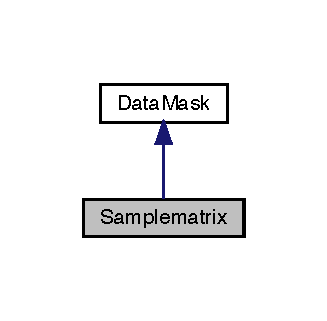
\includegraphics[width=157pt]{class_samplematrix__inherit__graph}
\end{center}
\end{figure}


Collaboration diagram for Samplematrix\+:
\nopagebreak
\begin{figure}[H]
\begin{center}
\leavevmode
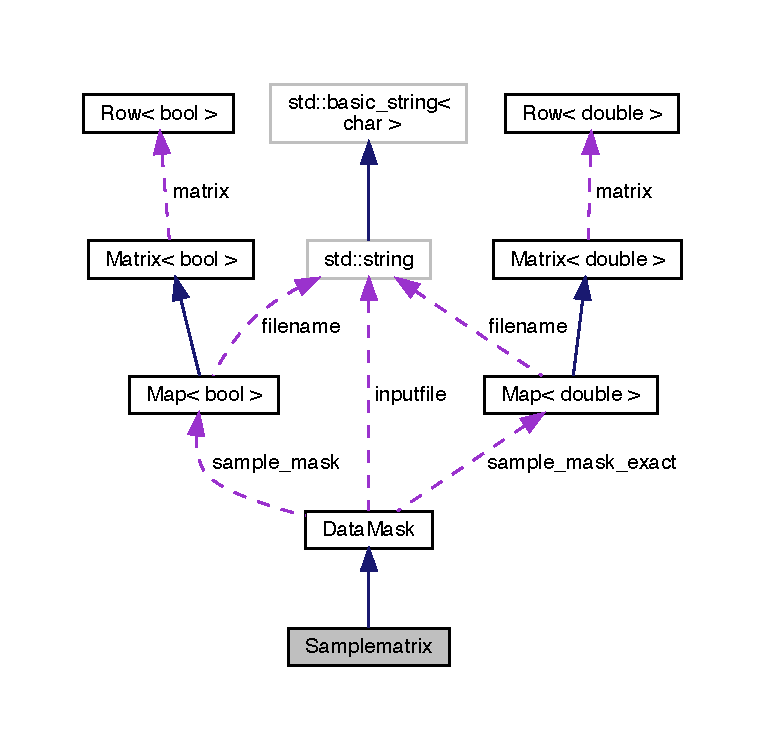
\includegraphics[width=174pt]{class_samplematrix__coll__graph}
\end{center}
\end{figure}
\subsection*{Public Member Functions}
\begin{DoxyCompactItemize}
\item 
\hyperlink{class_samplematrix_abe3fb4ca1e24678f2720f451cee80492}{Samplematrix} ()\hypertarget{class_samplematrix_abe3fb4ca1e24678f2720f451cee80492}{}\label{class_samplematrix_abe3fb4ca1e24678f2720f451cee80492}

\begin{DoxyCompactList}\small\item\em Inherit construction from the \hyperlink{class_matrix}{Matrix} class, but also set the booleans. \end{DoxyCompactList}\item 
bool \hyperlink{class_samplematrix_a834c750ab142d1ed2241fb9ab559b704}{get\+Test\+Val} (unsigned long xval, unsigned long yval, long xwrap, long ywrap)
\begin{DoxyCompactList}\small\item\em Returns the value at the x,y position. This is used for testing purposes only. \end{DoxyCompactList}\item 
bool \hyperlink{class_samplematrix_a8b494886260857ffdc9f52f47661a628}{get\+Mask\+Val} (unsigned long x1, unsigned long y1, long x\+\_\+wrap, long y\+\_\+wrap)
\begin{DoxyCompactList}\small\item\em Returns the value at the x,y position, with the given x and y wrap. Also checks whether or not the map is set to null, or whether the value comes from within a fragment. \end{DoxyCompactList}\item 
void \hyperlink{class_samplematrix_adbc1732a726c387965f63d4484bd4c25}{set\+Fragment} (\hyperlink{struct_fragment}{Fragment} \&fragment\+\_\+in)
\begin{DoxyCompactList}\small\item\em Set the fragment for the samplemask to some calculated fragment. This can be set multiple times. \end{DoxyCompactList}\item 
void \hyperlink{class_samplematrix_a9b796f2279f1716c2a555ff3d641ea0b}{remove\+Fragment} ()\hypertarget{class_samplematrix_a9b796f2279f1716c2a555ff3d641ea0b}{}\label{class_samplematrix_a9b796f2279f1716c2a555ff3d641ea0b}

\begin{DoxyCompactList}\small\item\em Removes the fragment. \end{DoxyCompactList}\item 
bool \hyperlink{class_data_mask_a093364b6da9442f7c4945b5a06cfe3af}{get\+Default} ()
\begin{DoxyCompactList}\small\item\em Returns if the simulation is using the a null samplemask, and therefore does not need to store the full sample grid in memory. \end{DoxyCompactList}\item 
bool \hyperlink{class_data_mask_a73922a90e7f491ec3dcf90fdd400fdf8}{setup} (const string \&sample\+\_\+mask\+\_\+file, const unsigned long \&x\+\_\+in, const unsigned long \&y\+\_\+in, const unsigned long \&mask\+\_\+x\+\_\+in, const unsigned long \&mask\+\_\+y\+\_\+in, const unsigned long \&x\+\_\+offset\+\_\+in, const unsigned long \&y\+\_\+offset\+\_\+in)
\begin{DoxyCompactList}\small\item\em Sets the parameters for the datamask, including the dimensions of the map, the offsets from the grid and the dimensions of the grid itself for recalculating coordinates. \end{DoxyCompactList}\item 
void \hyperlink{class_data_mask_a819eacf6968b0384a0221599dac09122}{import\+Boolean\+Mask} (unsigned long xdim, unsigned long ydim, unsigned long mask\+\_\+xdim, unsigned long mask\+\_\+ydim, unsigned long xoffset, unsigned long yoffset, string inputfile)
\begin{DoxyCompactList}\small\item\em Imports the sample mask as a boolean mask and sets the relevant sample mask dimensions. \end{DoxyCompactList}\item 
void \hyperlink{class_data_mask_a85f7b85bb4ac54aa884a8a06f1d35d1b}{do\+Import} ()\hypertarget{class_data_mask_a85f7b85bb4ac54aa884a8a06f1d35d1b}{}\label{class_data_mask_a85f7b85bb4ac54aa884a8a06f1d35d1b}

\begin{DoxyCompactList}\small\item\em Imports the boolean map object. \end{DoxyCompactList}\item 
void \hyperlink{class_data_mask_ac756e21b1c8d9412d565fb020eec9a06}{import\+Sample\+Mask} (\hyperlink{struct_sim_parameters}{Sim\+Parameters} \&mapvarin)
\begin{DoxyCompactList}\small\item\em Imports the specified file for the sampling percentage within each cell. \end{DoxyCompactList}\item 
bool \hyperlink{class_data_mask_ace6578db5b096b0c24112cc438cfa90d}{get\+Val} (const long \&x, const long \&y, const long \&xwrap, const long \&ywrap)
\begin{DoxyCompactList}\small\item\em Calculates the matrix value at the provided x, y location. If everywhere is sampled, simply returns true, as no sample\+\_\+mask will be stored in memory. This is to save R\+AM where possible. \end{DoxyCompactList}\item 
double \hyperlink{class_data_mask_af7a7cb35d309d37f42c7a3720a02b400}{get\+Null\+Proportion} (const long \&x, const long \&y, const long \&xwrap, const long \&ywrap)
\begin{DoxyCompactList}\small\item\em Separate return function for always returning 1.\+0 as density value. \end{DoxyCompactList}\item 
double \hyperlink{class_data_mask_a31cb42c363219967a7867340a7110e9f}{get\+Bool\+Proportion} (const long \&x, const long \&y, const long \&xwrap, const long \&ywrap)
\begin{DoxyCompactList}\small\item\em Returns the exact value from the spatial sampling map, for calculating the proportion of individuals to be sampled in each cell. \end{DoxyCompactList}\item 
double \hyperlink{class_data_mask_a682324892b67910b1dd2fa86a98c0873}{get\+Sample\+Proportion} (const long \&x, const long \&y, const long \&xwrap, const long \&ywrap)
\begin{DoxyCompactList}\small\item\em Returns the exact value from the spatial sampling map, for calculating the proportion of individuals to be sampled in each cell. \end{DoxyCompactList}\item 
double \hyperlink{class_data_mask_a2738d996bf7ee99d44a2833b2bed15ef}{get\+Exact\+Value} (const long \&x, const long \&y, const long \&xwrap, const long \&ywrap)
\begin{DoxyCompactList}\small\item\em Returns the exact value from the spatial sampling map, as returned by the pointer function. \end{DoxyCompactList}\item 
void \hyperlink{class_data_mask_a881c2393b1506d5dd026750405613bdd}{convert\+Boolean} (\hyperlink{class_landscape}{Landscape} \&map1, const double \&deme\+\_\+sampling, const double \&generation)
\begin{DoxyCompactList}\small\item\em Converts the spatial map into the boolean grid required for continued simulation. This is done so that the faster boolean accesses are possible. \end{DoxyCompactList}\item 
void \hyperlink{class_data_mask_a2d152bcb13820a9061ea85c984e042a7}{clear\+Spatial\+Mask} ()\hypertarget{class_data_mask_a2d152bcb13820a9061ea85c984e042a7}{}\label{class_data_mask_a2d152bcb13820a9061ea85c984e042a7}

\begin{DoxyCompactList}\small\item\em Removes the spatial mask from memory. This should be performed if no more map expansions are required. \end{DoxyCompactList}\item 
void \hyperlink{class_data_mask_ab96af629241f61a4d7122c6b7a91a3ef}{recalculate\+\_\+coordinates} (long \&x, long \&y, long \&x\+\_\+wrap, long \&y\+\_\+wrap)
\begin{DoxyCompactList}\small\item\em Converts the coordinates back into the grid format. Changes the values in the provided variables to be correct. \end{DoxyCompactList}\end{DoxyCompactItemize}
\subsection*{Public Attributes}
\begin{DoxyCompactItemize}
\item 
Map$<$ bool $>$ {\bfseries sample\+\_\+mask}\hypertarget{class_data_mask_a0ebe741d4b22824f93dacddd175d2c96}{}\label{class_data_mask_a0ebe741d4b22824f93dacddd175d2c96}

\item 
Map$<$ double $>$ \hyperlink{class_data_mask_acc231ebddc3e5db0103220b20d968a4f}{sample\+\_\+mask\+\_\+exact}
\end{DoxyCompactItemize}
\subsection*{Protected Types}
\begin{DoxyCompactItemize}
\item 
typedef double(Data\+Mask\+::$\ast$ {\bfseries fptr}) (const long \&x, const long \&y, const long \&xwrap, const long \&ywrap)\hypertarget{class_data_mask_a0ed51de5661fc3046d085e044a7efd4a}{}\label{class_data_mask_a0ed51de5661fc3046d085e044a7efd4a}

\end{DoxyCompactItemize}
\subsection*{Protected Attributes}
\begin{DoxyCompactItemize}
\item 
string {\bfseries inputfile}\hypertarget{class_data_mask_acde16cc845a6102a8b2ee0aa9b8917cb}{}\label{class_data_mask_acde16cc845a6102a8b2ee0aa9b8917cb}

\item 
bool {\bfseries b\+Default}\hypertarget{class_data_mask_af5d895b50f04eceac1e473dee6f36703}{}\label{class_data_mask_af5d895b50f04eceac1e473dee6f36703}

\item 
unsigned long {\bfseries x\+\_\+offset}\hypertarget{class_data_mask_a70178c907b2dc072b62f4bfb8f690823}{}\label{class_data_mask_a70178c907b2dc072b62f4bfb8f690823}

\item 
unsigned long {\bfseries y\+\_\+offset}\hypertarget{class_data_mask_ab4508058d8563d90bfc606a648cedb2f}{}\label{class_data_mask_ab4508058d8563d90bfc606a648cedb2f}

\item 
unsigned long {\bfseries x\+\_\+dim}\hypertarget{class_data_mask_aba77e907211dea06a4a52ad3036716b0}{}\label{class_data_mask_aba77e907211dea06a4a52ad3036716b0}

\item 
unsigned long {\bfseries y\+\_\+dim}\hypertarget{class_data_mask_aa2c689edd7b8bd84bb60e836aac4e378}{}\label{class_data_mask_aa2c689edd7b8bd84bb60e836aac4e378}

\item 
unsigned long {\bfseries mask\+\_\+x\+\_\+dim}\hypertarget{class_data_mask_ab971fd5a14a17e850cd92c79c3a1543e}{}\label{class_data_mask_ab971fd5a14a17e850cd92c79c3a1543e}

\item 
unsigned long {\bfseries mask\+\_\+y\+\_\+dim}\hypertarget{class_data_mask_a5ab1bf33e9b9fac964c8c2576fc5edca}{}\label{class_data_mask_a5ab1bf33e9b9fac964c8c2576fc5edca}

\item 
fptr {\bfseries get\+Proportionfptr}\hypertarget{class_data_mask_a67c92c63f3397de5312c573281515c1c}{}\label{class_data_mask_a67c92c63f3397de5312c573281515c1c}

\end{DoxyCompactItemize}


\subsection{Detailed Description}
A child of the \hyperlink{class_matrix}{Matrix} class as booleans. Used for determining where to sample species from. 

\subsection{Member Function Documentation}
\index{Samplematrix@{Samplematrix}!convert\+Boolean@{convert\+Boolean}}
\index{convert\+Boolean@{convert\+Boolean}!Samplematrix@{Samplematrix}}
\subsubsection[{\texorpdfstring{convert\+Boolean(\+Landscape \&map1, const double \&deme\+\_\+sampling, const double \&generation)}{convertBoolean(Landscape &map1, const double &deme_sampling, const double &generation)}}]{\setlength{\rightskip}{0pt plus 5cm}void Data\+Mask\+::convert\+Boolean (
\begin{DoxyParamCaption}
\item[{{\bf Landscape} \&}]{map1, }
\item[{const double \&}]{deme\+\_\+sampling, }
\item[{const double \&}]{generation}
\end{DoxyParamCaption}
)\hspace{0.3cm}{\ttfamily [inherited]}}\hypertarget{class_data_mask_a881c2393b1506d5dd026750405613bdd}{}\label{class_data_mask_a881c2393b1506d5dd026750405613bdd}


Converts the spatial map into the boolean grid required for continued simulation. This is done so that the faster boolean accesses are possible. 


\begin{DoxyParams}{Parameters}
{\em map1} & the map object to obtain density values from \\
\hline
{\em deme\+\_\+sampling} & the proportion of individuals to sample \\
\hline
{\em generation} & the generation individuals are added at \\
\hline
\end{DoxyParams}
\index{Samplematrix@{Samplematrix}!get\+Bool\+Proportion@{get\+Bool\+Proportion}}
\index{get\+Bool\+Proportion@{get\+Bool\+Proportion}!Samplematrix@{Samplematrix}}
\subsubsection[{\texorpdfstring{get\+Bool\+Proportion(const long \&x, const long \&y, const long \&xwrap, const long \&ywrap)}{getBoolProportion(const long &x, const long &y, const long &xwrap, const long &ywrap)}}]{\setlength{\rightskip}{0pt plus 5cm}double Data\+Mask\+::get\+Bool\+Proportion (
\begin{DoxyParamCaption}
\item[{const long \&}]{x, }
\item[{const long \&}]{y, }
\item[{const long \&}]{xwrap, }
\item[{const long \&}]{ywrap}
\end{DoxyParamCaption}
)\hspace{0.3cm}{\ttfamily [inherited]}}\hypertarget{class_data_mask_a31cb42c363219967a7867340a7110e9f}{}\label{class_data_mask_a31cb42c363219967a7867340a7110e9f}


Returns the exact value from the spatial sampling map, for calculating the proportion of individuals to be sampled in each cell. 

\begin{DoxyNote}{Note}
this function assumes that the file is not \char`\"{}null\char`\"{} and the exact sampling mask has been imported. No error checks on these conditions are performed except in debugging mode. 
\end{DoxyNote}

\begin{DoxyParams}{Parameters}
{\em x} & the x position on the grid \\
\hline
{\em y} & the y position on the grid \\
\hline
{\em xwrap} & the number of x wraps around the map \\
\hline
{\em ywrap} & the number of y wraps around the map \\
\hline
\end{DoxyParams}
\begin{DoxyReturn}{Returns}
the sample\+\_\+mask\+\_\+exact value at (x, y) 
\end{DoxyReturn}
\index{Samplematrix@{Samplematrix}!get\+Default@{get\+Default}}
\index{get\+Default@{get\+Default}!Samplematrix@{Samplematrix}}
\subsubsection[{\texorpdfstring{get\+Default()}{getDefault()}}]{\setlength{\rightskip}{0pt plus 5cm}bool Data\+Mask\+::get\+Default (
\begin{DoxyParamCaption}
{}
\end{DoxyParamCaption}
)\hspace{0.3cm}{\ttfamily [inherited]}}\hypertarget{class_data_mask_a093364b6da9442f7c4945b5a06cfe3af}{}\label{class_data_mask_a093364b6da9442f7c4945b5a06cfe3af}


Returns if the simulation is using the a null samplemask, and therefore does not need to store the full sample grid in memory. 

\begin{DoxyReturn}{Returns}
true if using a null samplemask 
\end{DoxyReturn}
\index{Samplematrix@{Samplematrix}!get\+Exact\+Value@{get\+Exact\+Value}}
\index{get\+Exact\+Value@{get\+Exact\+Value}!Samplematrix@{Samplematrix}}
\subsubsection[{\texorpdfstring{get\+Exact\+Value(const long \&x, const long \&y, const long \&xwrap, const long \&ywrap)}{getExactValue(const long &x, const long &y, const long &xwrap, const long &ywrap)}}]{\setlength{\rightskip}{0pt plus 5cm}double Data\+Mask\+::get\+Exact\+Value (
\begin{DoxyParamCaption}
\item[{const long \&}]{x, }
\item[{const long \&}]{y, }
\item[{const long \&}]{xwrap, }
\item[{const long \&}]{ywrap}
\end{DoxyParamCaption}
)\hspace{0.3cm}{\ttfamily [inherited]}}\hypertarget{class_data_mask_a2738d996bf7ee99d44a2833b2bed15ef}{}\label{class_data_mask_a2738d996bf7ee99d44a2833b2bed15ef}


Returns the exact value from the spatial sampling map, as returned by the pointer function. 


\begin{DoxyParams}{Parameters}
{\em x} & the x position on the grid \\
\hline
{\em y} & the y position on the grid \\
\hline
{\em xwrap} & the number of x wraps around the map \\
\hline
{\em ywrap} & the number of y wraps around the map \\
\hline
\end{DoxyParams}
\begin{DoxyReturn}{Returns}
the sample\+\_\+mask\+\_\+exact value at (x, y) 
\end{DoxyReturn}
\index{Samplematrix@{Samplematrix}!get\+Mask\+Val@{get\+Mask\+Val}}
\index{get\+Mask\+Val@{get\+Mask\+Val}!Samplematrix@{Samplematrix}}
\subsubsection[{\texorpdfstring{get\+Mask\+Val(unsigned long x1, unsigned long y1, long x\+\_\+wrap, long y\+\_\+wrap)}{getMaskVal(unsigned long x1, unsigned long y1, long x_wrap, long y_wrap)}}]{\setlength{\rightskip}{0pt plus 5cm}bool Samplematrix\+::get\+Mask\+Val (
\begin{DoxyParamCaption}
\item[{unsigned long}]{x1, }
\item[{unsigned long}]{y1, }
\item[{long}]{x\+\_\+wrap, }
\item[{long}]{y\+\_\+wrap}
\end{DoxyParamCaption}
)}\hypertarget{class_samplematrix_a8b494886260857ffdc9f52f47661a628}{}\label{class_samplematrix_a8b494886260857ffdc9f52f47661a628}


Returns the value at the x,y position, with the given x and y wrap. Also checks whether or not the map is set to null, or whether the value comes from within a fragment. 


\begin{DoxyParams}{Parameters}
{\em x1} & the x coordinate. \\
\hline
{\em y1} & the y coordinate \\
\hline
\end{DoxyParams}
\begin{DoxyReturn}{Returns}
the value at x,y. 
\end{DoxyReturn}
\index{Samplematrix@{Samplematrix}!get\+Null\+Proportion@{get\+Null\+Proportion}}
\index{get\+Null\+Proportion@{get\+Null\+Proportion}!Samplematrix@{Samplematrix}}
\subsubsection[{\texorpdfstring{get\+Null\+Proportion(const long \&x, const long \&y, const long \&xwrap, const long \&ywrap)}{getNullProportion(const long &x, const long &y, const long &xwrap, const long &ywrap)}}]{\setlength{\rightskip}{0pt plus 5cm}double Data\+Mask\+::get\+Null\+Proportion (
\begin{DoxyParamCaption}
\item[{const long \&}]{x, }
\item[{const long \&}]{y, }
\item[{const long \&}]{xwrap, }
\item[{const long \&}]{ywrap}
\end{DoxyParamCaption}
)\hspace{0.3cm}{\ttfamily [inherited]}}\hypertarget{class_data_mask_af7a7cb35d309d37f42c7a3720a02b400}{}\label{class_data_mask_af7a7cb35d309d37f42c7a3720a02b400}


Separate return function for always returning 1.\+0 as density value. 


\begin{DoxyParams}{Parameters}
{\em x} & the x position on the grid \\
\hline
{\em y} & the y position on the grid \\
\hline
{\em xwrap} & the number of x wraps around the map \\
\hline
{\em ywrap} & the number of y wraps around the map \\
\hline
\end{DoxyParams}
\begin{DoxyReturn}{Returns}
the sample\+\_\+mask\+\_\+exact value at (x, y) 
\end{DoxyReturn}
\index{Samplematrix@{Samplematrix}!get\+Sample\+Proportion@{get\+Sample\+Proportion}}
\index{get\+Sample\+Proportion@{get\+Sample\+Proportion}!Samplematrix@{Samplematrix}}
\subsubsection[{\texorpdfstring{get\+Sample\+Proportion(const long \&x, const long \&y, const long \&xwrap, const long \&ywrap)}{getSampleProportion(const long &x, const long &y, const long &xwrap, const long &ywrap)}}]{\setlength{\rightskip}{0pt plus 5cm}double Data\+Mask\+::get\+Sample\+Proportion (
\begin{DoxyParamCaption}
\item[{const long \&}]{x, }
\item[{const long \&}]{y, }
\item[{const long \&}]{xwrap, }
\item[{const long \&}]{ywrap}
\end{DoxyParamCaption}
)\hspace{0.3cm}{\ttfamily [inherited]}}\hypertarget{class_data_mask_a682324892b67910b1dd2fa86a98c0873}{}\label{class_data_mask_a682324892b67910b1dd2fa86a98c0873}


Returns the exact value from the spatial sampling map, for calculating the proportion of individuals to be sampled in each cell. 

\begin{DoxyNote}{Note}
this function assumes that the file is not \char`\"{}null\char`\"{} and the exact sampling mask has been imported. No error checks on these conditions are performed except in debugging mode. 
\end{DoxyNote}

\begin{DoxyParams}{Parameters}
{\em x} & the x position on the grid \\
\hline
{\em y} & the y position on the grid \\
\hline
{\em xwrap} & the number of x wraps around the map \\
\hline
{\em ywrap} & the number of y wraps around the map \\
\hline
\end{DoxyParams}
\begin{DoxyReturn}{Returns}
the sample\+\_\+mask\+\_\+exact value at (x, y) 
\end{DoxyReturn}
\index{Samplematrix@{Samplematrix}!get\+Test\+Val@{get\+Test\+Val}}
\index{get\+Test\+Val@{get\+Test\+Val}!Samplematrix@{Samplematrix}}
\subsubsection[{\texorpdfstring{get\+Test\+Val(unsigned long xval, unsigned long yval, long xwrap, long ywrap)}{getTestVal(unsigned long xval, unsigned long yval, long xwrap, long ywrap)}}]{\setlength{\rightskip}{0pt plus 5cm}bool Samplematrix\+::get\+Test\+Val (
\begin{DoxyParamCaption}
\item[{unsigned long}]{xval, }
\item[{unsigned long}]{yval, }
\item[{long}]{xwrap, }
\item[{long}]{ywrap}
\end{DoxyParamCaption}
)}\hypertarget{class_samplematrix_a834c750ab142d1ed2241fb9ab559b704}{}\label{class_samplematrix_a834c750ab142d1ed2241fb9ab559b704}


Returns the value at the x,y position. This is used for testing purposes only. 


\begin{DoxyParams}{Parameters}
{\em xval} & the x coordinate. \\
\hline
{\em yval} & the y coordinate \\
\hline
{\em xwrap} & the x wrapping \\
\hline
{\em ywrap} & the y wrapping \\
\hline
\end{DoxyParams}
\begin{DoxyReturn}{Returns}
the value at x,y. 
\end{DoxyReturn}
\index{Samplematrix@{Samplematrix}!get\+Val@{get\+Val}}
\index{get\+Val@{get\+Val}!Samplematrix@{Samplematrix}}
\subsubsection[{\texorpdfstring{get\+Val(const long \&x, const long \&y, const long \&xwrap, const long \&ywrap)}{getVal(const long &x, const long &y, const long &xwrap, const long &ywrap)}}]{\setlength{\rightskip}{0pt plus 5cm}bool Data\+Mask\+::get\+Val (
\begin{DoxyParamCaption}
\item[{const long \&}]{x, }
\item[{const long \&}]{y, }
\item[{const long \&}]{xwrap, }
\item[{const long \&}]{ywrap}
\end{DoxyParamCaption}
)\hspace{0.3cm}{\ttfamily [inherited]}}\hypertarget{class_data_mask_ace6578db5b096b0c24112cc438cfa90d}{}\label{class_data_mask_ace6578db5b096b0c24112cc438cfa90d}


Calculates the matrix value at the provided x, y location. If everywhere is sampled, simply returns true, as no sample\+\_\+mask will be stored in memory. This is to save R\+AM where possible. 


\begin{DoxyParams}{Parameters}
{\em x} & the x position on the grid \\
\hline
{\em y} & the y position on the grid \\
\hline
{\em xval} & the number of x wraps \\
\hline
{\em yval} & the number of y wraps \\
\hline
\end{DoxyParams}
\begin{DoxyReturn}{Returns}
the sample\+\_\+mask value at x,y (or true if the file was \char`\"{}null\char`\"{}) 
\end{DoxyReturn}
\index{Samplematrix@{Samplematrix}!import\+Boolean\+Mask@{import\+Boolean\+Mask}}
\index{import\+Boolean\+Mask@{import\+Boolean\+Mask}!Samplematrix@{Samplematrix}}
\subsubsection[{\texorpdfstring{import\+Boolean\+Mask(unsigned long xdim, unsigned long ydim, unsigned long mask\+\_\+xdim, unsigned long mask\+\_\+ydim, unsigned long xoffset, unsigned long yoffset, string inputfile)}{importBooleanMask(unsigned long xdim, unsigned long ydim, unsigned long mask_xdim, unsigned long mask_ydim, unsigned long xoffset, unsigned long yoffset, string inputfile)}}]{\setlength{\rightskip}{0pt plus 5cm}void Data\+Mask\+::import\+Boolean\+Mask (
\begin{DoxyParamCaption}
\item[{unsigned long}]{xdim, }
\item[{unsigned long}]{ydim, }
\item[{unsigned long}]{mask\+\_\+xdim, }
\item[{unsigned long}]{mask\+\_\+ydim, }
\item[{unsigned long}]{xoffset, }
\item[{unsigned long}]{yoffset, }
\item[{string}]{inputfile}
\end{DoxyParamCaption}
)\hspace{0.3cm}{\ttfamily [inherited]}}\hypertarget{class_data_mask_a819eacf6968b0384a0221599dac09122}{}\label{class_data_mask_a819eacf6968b0384a0221599dac09122}


Imports the sample mask as a boolean mask and sets the relevant sample mask dimensions. 


\begin{DoxyParams}{Parameters}
{\em xdim} & the x dimension of the grid area \\
\hline
{\em ydim} & the y dimension of the grid area \\
\hline
{\em mask\+\_\+xdim} & the x dimension of the sample map file \\
\hline
{\em mask\+\_\+ydim} & the y dimension of the sample map file \\
\hline
{\em xoffset} & the x offset of the grid area from the sample map file \\
\hline
{\em yoffset} & the y offset of the grid area from the sample map file \\
\hline
{\em inputfile} & the path to the sample map file \\
\hline
\end{DoxyParams}
\index{Samplematrix@{Samplematrix}!import\+Sample\+Mask@{import\+Sample\+Mask}}
\index{import\+Sample\+Mask@{import\+Sample\+Mask}!Samplematrix@{Samplematrix}}
\subsubsection[{\texorpdfstring{import\+Sample\+Mask(\+Sim\+Parameters \&mapvarin)}{importSampleMask(SimParameters &mapvarin)}}]{\setlength{\rightskip}{0pt plus 5cm}void Data\+Mask\+::import\+Sample\+Mask (
\begin{DoxyParamCaption}
\item[{{\bf Sim\+Parameters} \&}]{mapvarin}
\end{DoxyParamCaption}
)\hspace{0.3cm}{\ttfamily [inherited]}}\hypertarget{class_data_mask_ac756e21b1c8d9412d565fb020eec9a06}{}\label{class_data_mask_ac756e21b1c8d9412d565fb020eec9a06}


Imports the specified file for the sampling percentage within each cell. 

The map should consist of floating points representing the relative sampling rates in each cell. Note that the actual sampling proportion is equal to the cell value multiplied by global deme sampling proportion. 
\begin{DoxyParams}{Parameters}
{\em mapvarin} & the \hyperlink{struct_sim_parameters}{Sim\+Parameters} object containing the samplemask file location and dimensions \\
\hline
\end{DoxyParams}
\index{Samplematrix@{Samplematrix}!recalculate\+\_\+coordinates@{recalculate\+\_\+coordinates}}
\index{recalculate\+\_\+coordinates@{recalculate\+\_\+coordinates}!Samplematrix@{Samplematrix}}
\subsubsection[{\texorpdfstring{recalculate\+\_\+coordinates(long \&x, long \&y, long \&x\+\_\+wrap, long \&y\+\_\+wrap)}{recalculate_coordinates(long &x, long &y, long &x_wrap, long &y_wrap)}}]{\setlength{\rightskip}{0pt plus 5cm}void Data\+Mask\+::recalculate\+\_\+coordinates (
\begin{DoxyParamCaption}
\item[{long \&}]{x, }
\item[{long \&}]{y, }
\item[{long \&}]{x\+\_\+wrap, }
\item[{long \&}]{y\+\_\+wrap}
\end{DoxyParamCaption}
)\hspace{0.3cm}{\ttfamily [inherited]}}\hypertarget{class_data_mask_ab96af629241f61a4d7122c6b7a91a3ef}{}\label{class_data_mask_ab96af629241f61a4d7122c6b7a91a3ef}


Converts the coordinates back into the grid format. Changes the values in the provided variables to be correct. 


\begin{DoxyParams}{Parameters}
{\em x} & the x value to convert \\
\hline
{\em y} & the y value to convert \\
\hline
{\em x\+\_\+wrap} & the xwrap variable to place the value into \\
\hline
{\em y\+\_\+wrap} & the ywrap variable to place the value into \\
\hline
\end{DoxyParams}
\index{Samplematrix@{Samplematrix}!set\+Fragment@{set\+Fragment}}
\index{set\+Fragment@{set\+Fragment}!Samplematrix@{Samplematrix}}
\subsubsection[{\texorpdfstring{set\+Fragment(\+Fragment \&fragment\+\_\+in)}{setFragment(Fragment &fragment_in)}}]{\setlength{\rightskip}{0pt plus 5cm}void Samplematrix\+::set\+Fragment (
\begin{DoxyParamCaption}
\item[{{\bf Fragment} \&}]{fragment\+\_\+in}
\end{DoxyParamCaption}
)}\hypertarget{class_samplematrix_adbc1732a726c387965f63d4484bd4c25}{}\label{class_samplematrix_adbc1732a726c387965f63d4484bd4c25}


Set the fragment for the samplemask to some calculated fragment. This can be set multiple times. 


\begin{DoxyParams}{Parameters}
{\em fragment\+\_\+in} & the \hyperlink{struct_fragment}{Fragment} to set the samplemask to. \\
\hline
\end{DoxyParams}
\index{Samplematrix@{Samplematrix}!setup@{setup}}
\index{setup@{setup}!Samplematrix@{Samplematrix}}
\subsubsection[{\texorpdfstring{setup(const string \&sample\+\_\+mask\+\_\+file, const unsigned long \&x\+\_\+in, const unsigned long \&y\+\_\+in, const unsigned long \&mask\+\_\+x\+\_\+in, const unsigned long \&mask\+\_\+y\+\_\+in, const unsigned long \&x\+\_\+offset\+\_\+in, const unsigned long \&y\+\_\+offset\+\_\+in)}{setup(const string &sample_mask_file, const unsigned long &x_in, const unsigned long &y_in, const unsigned long &mask_x_in, const unsigned long &mask_y_in, const unsigned long &x_offset_in, const unsigned long &y_offset_in)}}]{\setlength{\rightskip}{0pt plus 5cm}bool Data\+Mask\+::setup (
\begin{DoxyParamCaption}
\item[{const string \&}]{sample\+\_\+mask\+\_\+file, }
\item[{const unsigned long \&}]{x\+\_\+in, }
\item[{const unsigned long \&}]{y\+\_\+in, }
\item[{const unsigned long \&}]{mask\+\_\+x\+\_\+in, }
\item[{const unsigned long \&}]{mask\+\_\+y\+\_\+in, }
\item[{const unsigned long \&}]{x\+\_\+offset\+\_\+in, }
\item[{const unsigned long \&}]{y\+\_\+offset\+\_\+in}
\end{DoxyParamCaption}
)\hspace{0.3cm}{\ttfamily [inherited]}}\hypertarget{class_data_mask_a73922a90e7f491ec3dcf90fdd400fdf8}{}\label{class_data_mask_a73922a90e7f491ec3dcf90fdd400fdf8}


Sets the parameters for the datamask, including the dimensions of the map, the offsets from the grid and the dimensions of the grid itself for recalculating coordinates. 


\begin{DoxyParams}{Parameters}
{\em sample\+\_\+mask\+\_\+file} & the file to import the samplemask from (or \char`\"{}null\char`\"{}) \\
\hline
{\em x\+\_\+in} & x dimension of the grid \\
\hline
{\em y\+\_\+in} & y dimension of the grid \\
\hline
{\em mask\+\_\+x\+\_\+in} & x dimension of the sample mask \\
\hline
{\em mask\+\_\+y\+\_\+in} & y dimension of the sample mask \\
\hline
{\em x\+\_\+offset\+\_\+in} & x offset of the sample mask from the grid \\
\hline
{\em y\+\_\+offset\+\_\+in} & y offset of the sample mask from the grid \\
\hline
\end{DoxyParams}
\begin{DoxyReturn}{Returns}
true if using a \char`\"{}null\char`\"{} samplemask 
\end{DoxyReturn}


\subsection{Member Data Documentation}
\index{Samplematrix@{Samplematrix}!sample\+\_\+mask\+\_\+exact@{sample\+\_\+mask\+\_\+exact}}
\index{sample\+\_\+mask\+\_\+exact@{sample\+\_\+mask\+\_\+exact}!Samplematrix@{Samplematrix}}
\subsubsection[{\texorpdfstring{sample\+\_\+mask\+\_\+exact}{sample_mask_exact}}]{\setlength{\rightskip}{0pt plus 5cm}Map$<$double$>$ Data\+Mask\+::sample\+\_\+mask\+\_\+exact\hspace{0.3cm}{\ttfamily [inherited]}}\hypertarget{class_data_mask_acc231ebddc3e5db0103220b20d968a4f}{}\label{class_data_mask_acc231ebddc3e5db0103220b20d968a4f}
A binary grid telling whether or not the cell should be sampled. 

The documentation for this class was generated from the following files\+:\begin{DoxyCompactItemize}
\item 
necsim/Community.\+h\item 
necsim/Community.\+cpp\end{DoxyCompactItemize}

\hypertarget{struct_section_option}{}\section{Section\+Option Struct Reference}
\label{struct_section_option}\index{Section\+Option@{Section\+Option}}


A simple container for importing options from a config file.  




{\ttfamily \#include $<$Config\+File\+Parser.\+h$>$}



Collaboration diagram for Section\+Option\+:
\nopagebreak
\begin{figure}[H]
\begin{center}
\leavevmode
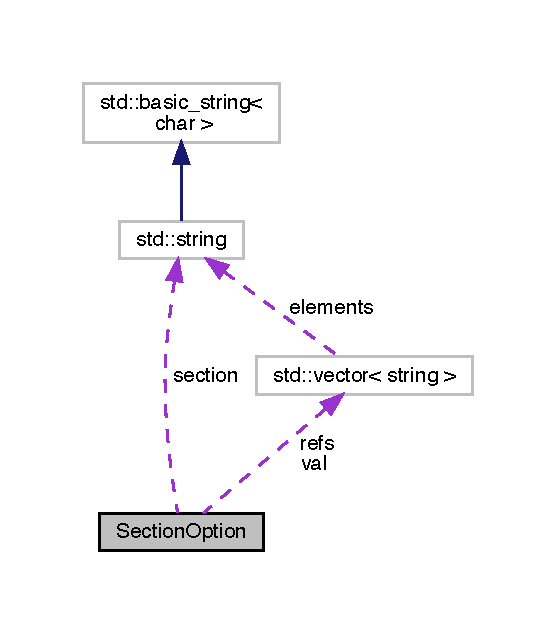
\includegraphics[width=267pt]{struct_section_option__coll__graph}
\end{center}
\end{figure}
\subsection*{Public Member Functions}
\begin{DoxyCompactItemize}
\item 
\hyperlink{struct_section_option_a0a6a33e41311ea0eef34b76379421362}{Section\+Option} ()\hypertarget{struct_section_option_a0a6a33e41311ea0eef34b76379421362}{}\label{struct_section_option_a0a6a33e41311ea0eef34b76379421362}

\begin{DoxyCompactList}\small\item\em Default constructor for \hyperlink{struct_section_option}{Section\+Option}. \end{DoxyCompactList}\item 
string \hyperlink{struct_section_option_a78d55aa842ba2056764236246492734f}{get\+Option} (string refval)
\begin{DoxyCompactList}\small\item\em Returns the value for the provided reference from within the key. \end{DoxyCompactList}\end{DoxyCompactItemize}
\subsection*{Public Attributes}
\begin{DoxyCompactItemize}
\item 
string {\bfseries section}\hypertarget{struct_section_option_af6dd28af164466810fe9f36091b9d6d1}{}\label{struct_section_option_af6dd28af164466810fe9f36091b9d6d1}

\item 
vector$<$ string $>$ {\bfseries val}\hypertarget{struct_section_option_a789da4aa7aeef3887bcfc94f7cf2c254}{}\label{struct_section_option_a789da4aa7aeef3887bcfc94f7cf2c254}

\item 
vector$<$ string $>$ {\bfseries refs}\hypertarget{struct_section_option_a916b36005e0e1817a9dcf45bf02952e4}{}\label{struct_section_option_a916b36005e0e1817a9dcf45bf02952e4}

\end{DoxyCompactItemize}
\subsection*{Friends}
\begin{DoxyCompactItemize}
\item 
ostream \& \hyperlink{struct_section_option_a8e9eafe82f001a7bf599bebb1f0bdb76}{operator$<$$<$} (ostream \&os, const \hyperlink{struct_section_option}{Section\+Option} \&k)
\begin{DoxyCompactList}\small\item\em Overloading the $<$$<$ operator for outputting to the output stream. \end{DoxyCompactList}\item 
istream \& \hyperlink{struct_section_option_a6e317b3e4692b867e48205afcceff1a1}{operator$>$$>$} (istream \&is, \hyperlink{struct_section_option}{Section\+Option} \&k)
\begin{DoxyCompactList}\small\item\em Overloading the $>$$>$ operator for inputting from an input stream. \end{DoxyCompactList}\end{DoxyCompactItemize}


\subsection{Detailed Description}
A simple container for importing options from a config file. 

\subsection{Member Function Documentation}
\index{Section\+Option@{Section\+Option}!get\+Option@{get\+Option}}
\index{get\+Option@{get\+Option}!Section\+Option@{Section\+Option}}
\subsubsection[{\texorpdfstring{get\+Option(string refval)}{getOption(string refval)}}]{\setlength{\rightskip}{0pt plus 5cm}string Section\+Option\+::get\+Option (
\begin{DoxyParamCaption}
\item[{string}]{refval}
\end{DoxyParamCaption}
)}\hypertarget{struct_section_option_a78d55aa842ba2056764236246492734f}{}\label{struct_section_option_a78d55aa842ba2056764236246492734f}


Returns the value for the provided reference from within the key. 


\begin{DoxyParams}{Parameters}
{\em refval} & the reference to obtain the value of \\
\hline
\end{DoxyParams}
\begin{DoxyReturn}{Returns}
the requested value as a string. Returns string \char`\"{}null\char`\"{} if no reference is found. 
\end{DoxyReturn}


\subsection{Friends And Related Function Documentation}
\index{Section\+Option@{Section\+Option}!operator$<$$<$@{operator$<$$<$}}
\index{operator$<$$<$@{operator$<$$<$}!Section\+Option@{Section\+Option}}
\subsubsection[{\texorpdfstring{operator$<$$<$}{operator<<}}]{\setlength{\rightskip}{0pt plus 5cm}ostream\& operator$<$$<$ (
\begin{DoxyParamCaption}
\item[{ostream \&}]{os, }
\item[{const {\bf Section\+Option} \&}]{k}
\end{DoxyParamCaption}
)\hspace{0.3cm}{\ttfamily [friend]}}\hypertarget{struct_section_option_a8e9eafe82f001a7bf599bebb1f0bdb76}{}\label{struct_section_option_a8e9eafe82f001a7bf599bebb1f0bdb76}


Overloading the $<$$<$ operator for outputting to the output stream. 


\begin{DoxyParams}{Parameters}
{\em os} & the output stream. \\
\hline
{\em k} & the Key\+Option object. \\
\hline
\end{DoxyParams}
\begin{DoxyReturn}{Returns}
os the output stream. 
\end{DoxyReturn}
\index{Section\+Option@{Section\+Option}!operator$>$$>$@{operator$>$$>$}}
\index{operator$>$$>$@{operator$>$$>$}!Section\+Option@{Section\+Option}}
\subsubsection[{\texorpdfstring{operator$>$$>$}{operator>>}}]{\setlength{\rightskip}{0pt plus 5cm}istream\& operator$>$$>$ (
\begin{DoxyParamCaption}
\item[{istream \&}]{is, }
\item[{{\bf Section\+Option} \&}]{k}
\end{DoxyParamCaption}
)\hspace{0.3cm}{\ttfamily [friend]}}\hypertarget{struct_section_option_a6e317b3e4692b867e48205afcceff1a1}{}\label{struct_section_option_a6e317b3e4692b867e48205afcceff1a1}


Overloading the $>$$>$ operator for inputting from an input stream. 


\begin{DoxyParams}{Parameters}
{\em is} & the input stream \\
\hline
{\em k} & the Key\+Option object \\
\hline
\end{DoxyParams}
\begin{DoxyReturn}{Returns}
is the input stream 
\end{DoxyReturn}


The documentation for this struct was generated from the following files\+:\begin{DoxyCompactItemize}
\item 
necsim/Config\+File\+Parser.\+h\item 
necsim/Config\+File\+Parser.\+cpp\end{DoxyCompactItemize}

\hypertarget{struct_sim_parameters}{}\section{Sim\+Parameters Struct Reference}
\label{struct_sim_parameters}\index{Sim\+Parameters@{Sim\+Parameters}}


Stores and imports the variables required by the Map object. Used to setting the Map variables in a more elegant way.  




{\ttfamily \#include $<$Sim\+Parameters.\+h$>$}



Collaboration diagram for Sim\+Parameters\+:
\nopagebreak
\begin{figure}[H]
\begin{center}
\leavevmode
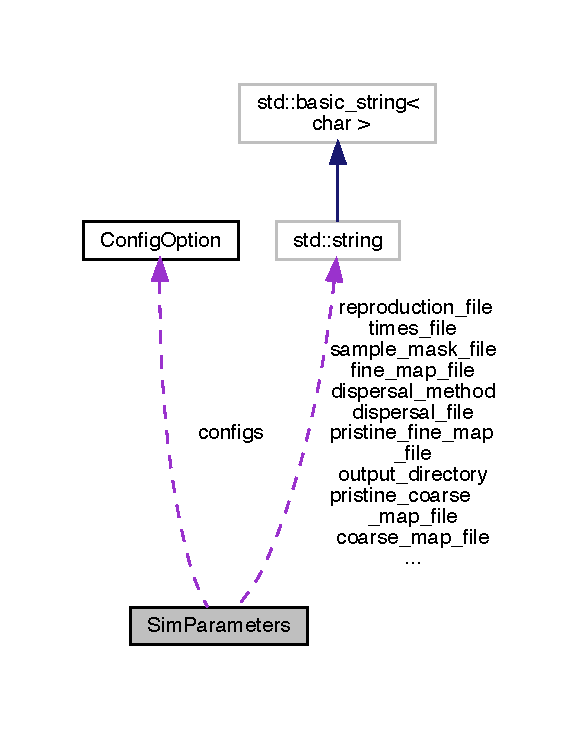
\includegraphics[width=350pt]{struct_sim_parameters__coll__graph}
\end{center}
\end{figure}
\subsection*{Public Member Functions}
\begin{DoxyCompactItemize}
\item 
\hyperlink{struct_sim_parameters_aa91bc46ea6909abeeb7488c36da269ee}{Sim\+Parameters} ()\hypertarget{struct_sim_parameters_aa91bc46ea6909abeeb7488c36da269ee}{}\label{struct_sim_parameters_aa91bc46ea6909abeeb7488c36da269ee}

\begin{DoxyCompactList}\small\item\em Default constructor. \end{DoxyCompactList}\item 
void \hyperlink{struct_sim_parameters_affb4a6133434c61c720b648012ccbcea}{import\+Parameters} (\hyperlink{class_config_option}{Config\+Option} $\ast$config\+Option)
\begin{DoxyCompactList}\small\item\em Links to the provided \hyperlink{class_config_option}{Config\+Option}. Assumes that the parameters have already been parsed from the config file. \end{DoxyCompactList}\item 
void \hyperlink{struct_sim_parameters_a2c587f1f41e13c51696ca24e5edadc96}{import\+Parameters} (const string \&conf\+\_\+in)
\begin{DoxyCompactList}\small\item\em Imports the spatial variables from a path to the config file.. \end{DoxyCompactList}\item 
void \hyperlink{struct_sim_parameters_a65833f22d1f30997727ed71e989af02e}{import\+Parameters} ()\hypertarget{struct_sim_parameters_a65833f22d1f30997727ed71e989af02e}{}\label{struct_sim_parameters_a65833f22d1f30997727ed71e989af02e}

\begin{DoxyCompactList}\small\item\em Main import of parameters from the config file option. \end{DoxyCompactList}\item 
void \hyperlink{struct_sim_parameters_aa6684caccd53613a5d08ff4071d0edc9}{set\+Key\+Parameters} (const long long \&task\+\_\+in, const long long \&seed\+\_\+in, const string \&output\+\_\+directory\+\_\+in, const unsigned long \&max\+\_\+time\+\_\+in, unsigned long desired\+\_\+specnum\+\_\+in, const string \&times\+\_\+file\+\_\+in)
\begin{DoxyCompactList}\small\item\em Sets the main simulation parameters. \end{DoxyCompactList}\item 
void \hyperlink{struct_sim_parameters_a6753a70e7b9183c97fb1b304b089968d}{set\+Speciation\+Parameters} (const long double \&spec\+\_\+in, bool is\+\_\+protracted\+\_\+in, const double \&min\+\_\+speciation\+\_\+gen\+\_\+in, const double \&max\+\_\+speciation\+\_\+gen\+\_\+in)
\begin{DoxyCompactList}\small\item\em Sets the speciation parameters for the simulation. \end{DoxyCompactList}\item 
void \hyperlink{struct_sim_parameters_a74782aab11b1e07a507cc60bdec3bf95}{set\+Dispersal\+Parameters} (const string \&dispersal\+\_\+method\+\_\+in, const double \&sigma\+\_\+in, const double \&tau\+\_\+in, const double \&m\+\_\+prob\+\_\+in, const double \&cutoff\+\_\+in, const double \&dispersal\+\_\+relative\+\_\+cost\+\_\+in, bool restrict\+\_\+self\+\_\+in, const string \&landscape\+\_\+type\+\_\+in, const string \&dispersal\+\_\+file\+\_\+in, const string \&reproduction\+\_\+file\+\_\+in)
\begin{DoxyCompactList}\small\item\em Sets the dispersal parameters for the simulation. \end{DoxyCompactList}\item 
void \hyperlink{struct_sim_parameters_afae472eb2788205a8587db87778f0333}{set\+Historical\+Map\+Parameters} (const string \&historical\+\_\+fine\+\_\+file\+\_\+map\+\_\+in, const string \&historical\+\_\+coarse\+\_\+map\+\_\+file\+\_\+in, const double \&gen\+\_\+since\+\_\+historical\+\_\+in, const double \&habitat\+\_\+change\+\_\+rate\+\_\+in)
\begin{DoxyCompactList}\small\item\em Sets the historical map parameters for the simulation. \end{DoxyCompactList}\item 
void {\bfseries set\+Historical\+Map\+Parameters} (vector$<$ string $>$ path\+\_\+fine, vector$<$ unsigned long $>$ number\+\_\+fine, vector$<$ double $>$ rate\+\_\+fine, vector$<$ double $>$ time\+\_\+fine, vector$<$ string $>$ path\+\_\+coarse, vector$<$ unsigned long $>$ number\+\_\+coarse, vector$<$ double $>$ rate\+\_\+coarse, vector$<$ double $>$ time\+\_\+coarse)\hypertarget{struct_sim_parameters_ae86196bee7f469e308d23e7dbbf7320c}{}\label{struct_sim_parameters_ae86196bee7f469e308d23e7dbbf7320c}

\item 
void \hyperlink{struct_sim_parameters_a4073ee2bf48a25eebdc0439e3b8625e7}{set\+Map\+Parameters} (const string \&fine\+\_\+map\+\_\+file\+\_\+in, const string \&coarse\+\_\+map\+\_\+file\+\_\+in, const string \&sample\+\_\+mask\+\_\+file\+\_\+in, const unsigned long \&grid\+\_\+x\+\_\+size\+\_\+in, const unsigned long \&grid\+\_\+y\+\_\+size\+\_\+in, const unsigned long \&sample\+\_\+x\+\_\+size\+\_\+in, const unsigned long \&sample\+\_\+y\+\_\+size\+\_\+in, const unsigned long \&sample\+\_\+x\+\_\+offset\+\_\+in, const unsigned long \&sample\+\_\+y\+\_\+offset\+\_\+in, const unsigned long \&fine\+\_\+map\+\_\+x\+\_\+size\+\_\+in, const unsigned long \&fine\+\_\+map\+\_\+y\+\_\+size\+\_\+in, const unsigned long \&fine\+\_\+map\+\_\+x\+\_\+offset\+\_\+in, const unsigned long \&fine\+\_\+map\+\_\+y\+\_\+offset\+\_\+in, const unsigned long \&coarse\+\_\+map\+\_\+x\+\_\+size\+\_\+in, const unsigned long \&coarse\+\_\+map\+\_\+y\+\_\+size\+\_\+in, const unsigned long \&coarse\+\_\+map\+\_\+x\+\_\+offset\+\_\+in, const unsigned long \&coarse\+\_\+map\+\_\+y\+\_\+offset\+\_\+in, const unsigned long \&coarse\+\_\+map\+\_\+scale\+\_\+in, const unsigned long \&deme\+\_\+in, const double \&deme\+\_\+sample\+\_\+in, bool uses\+\_\+spatial\+\_\+sampling\+\_\+in)
\begin{DoxyCompactList}\small\item\em Sets the map parameters for the simulation. \end{DoxyCompactList}\item 
bool \hyperlink{struct_sim_parameters_adae32b41ebc9b9bd0ae89ceb039430b4}{set\+Historical} (unsigned int n)
\begin{DoxyCompactList}\small\item\em Alters the historical parameters to the configuration matching the input number. If no configuration option exists for this number, is\+\_\+historical will be set to true. \end{DoxyCompactList}\item 
void \hyperlink{struct_sim_parameters_ac7072f58a9dccc718341d25a84148ffc}{print\+Vars} ()\hypertarget{struct_sim_parameters_ac7072f58a9dccc718341d25a84148ffc}{}\label{struct_sim_parameters_ac7072f58a9dccc718341d25a84148ffc}

\begin{DoxyCompactList}\small\item\em Prints selected important variables to the terminal. \end{DoxyCompactList}\item 
void \hyperlink{struct_sim_parameters_a04636fc2b0899400011b54bb1f175eb0}{print\+Spatial\+Vars} ()\hypertarget{struct_sim_parameters_a04636fc2b0899400011b54bb1f175eb0}{}\label{struct_sim_parameters_a04636fc2b0899400011b54bb1f175eb0}

\begin{DoxyCompactList}\small\item\em Prints the spatial variables. \end{DoxyCompactList}\item 
void {\bfseries set\+Metacommunity\+Parameters} (const unsigned long \&metacommunity\+\_\+size, const double \&speciation\+\_\+rate, const unsigned long \&seed, const unsigned long \&job)\hypertarget{struct_sim_parameters_a8a245d9aef5595c7d3b4e29e3b1a2ef2}{}\label{struct_sim_parameters_a8a245d9aef5595c7d3b4e29e3b1a2ef2}

\end{DoxyCompactItemize}
\subsection*{Public Attributes}
\begin{DoxyCompactItemize}
\item 
string {\bfseries fine\+\_\+map\+\_\+file}\hypertarget{struct_sim_parameters_a24483485b1127d7c4a91f02bd56a130e}{}\label{struct_sim_parameters_a24483485b1127d7c4a91f02bd56a130e}

\item 
string {\bfseries coarse\+\_\+map\+\_\+file}\hypertarget{struct_sim_parameters_a03831d4d7590072a153620fdedd7e2fd}{}\label{struct_sim_parameters_a03831d4d7590072a153620fdedd7e2fd}

\item 
string {\bfseries output\+\_\+directory}\hypertarget{struct_sim_parameters_afc36bb2fbfc7ebf5e84149be5be87c1e}{}\label{struct_sim_parameters_afc36bb2fbfc7ebf5e84149be5be87c1e}

\item 
string {\bfseries historical\+\_\+fine\+\_\+map\+\_\+file}\hypertarget{struct_sim_parameters_a0904ed1272de111c9e80c22dcdb2e039}{}\label{struct_sim_parameters_a0904ed1272de111c9e80c22dcdb2e039}

\item 
string {\bfseries historical\+\_\+coarse\+\_\+map\+\_\+file}\hypertarget{struct_sim_parameters_a621bfeaf44861f6b88d4117bc7da5a2b}{}\label{struct_sim_parameters_a621bfeaf44861f6b88d4117bc7da5a2b}

\item 
string {\bfseries sample\+\_\+mask\+\_\+file}\hypertarget{struct_sim_parameters_ac5298525ed1d094d1668bc78491b0c69}{}\label{struct_sim_parameters_ac5298525ed1d094d1668bc78491b0c69}

\item 
long long {\bfseries the\+\_\+task} \{\}\hypertarget{struct_sim_parameters_a219ea06b17e82f1512e0e8cdd9990ea7}{}\label{struct_sim_parameters_a219ea06b17e82f1512e0e8cdd9990ea7}

\item 
long long {\bfseries the\+\_\+seed} \{\}\hypertarget{struct_sim_parameters_a689610f6fd7c87866ca950c8700b4943}{}\label{struct_sim_parameters_a689610f6fd7c87866ca950c8700b4943}

\item 
unsigned long {\bfseries grid\+\_\+x\+\_\+size} \{\}\hypertarget{struct_sim_parameters_aba773a5ec7ad130d6009d319c7d2f591}{}\label{struct_sim_parameters_aba773a5ec7ad130d6009d319c7d2f591}

\item 
unsigned long {\bfseries grid\+\_\+y\+\_\+size} \{\}\hypertarget{struct_sim_parameters_a3d52bbca2ec77eb584b2940fce8b018f}{}\label{struct_sim_parameters_a3d52bbca2ec77eb584b2940fce8b018f}

\item 
unsigned long {\bfseries sample\+\_\+x\+\_\+size} \{\}\hypertarget{struct_sim_parameters_ae5b4ec9858fdeb80231ad20a255402ee}{}\label{struct_sim_parameters_ae5b4ec9858fdeb80231ad20a255402ee}

\item 
unsigned long {\bfseries sample\+\_\+y\+\_\+size} \{\}\hypertarget{struct_sim_parameters_a81ffb850421d1e758c770fdbba39ed67}{}\label{struct_sim_parameters_a81ffb850421d1e758c770fdbba39ed67}

\item 
unsigned long {\bfseries sample\+\_\+x\+\_\+offset} \{\}\hypertarget{struct_sim_parameters_a8f303a960065679ea0d5fcb3c85f87f6}{}\label{struct_sim_parameters_a8f303a960065679ea0d5fcb3c85f87f6}

\item 
unsigned long {\bfseries sample\+\_\+y\+\_\+offset} \{\}\hypertarget{struct_sim_parameters_ab6bc36c5ef40d86635116626964da79a}{}\label{struct_sim_parameters_ab6bc36c5ef40d86635116626964da79a}

\item 
unsigned long {\bfseries fine\+\_\+map\+\_\+x\+\_\+size} \{\}\hypertarget{struct_sim_parameters_aec1386c872750e502b69c3037afdba2f}{}\label{struct_sim_parameters_aec1386c872750e502b69c3037afdba2f}

\item 
unsigned long {\bfseries fine\+\_\+map\+\_\+y\+\_\+size} \{\}\hypertarget{struct_sim_parameters_ad810612827e11f079e8a5c57bc4fabed}{}\label{struct_sim_parameters_ad810612827e11f079e8a5c57bc4fabed}

\item 
unsigned long {\bfseries fine\+\_\+map\+\_\+x\+\_\+offset} \{\}\hypertarget{struct_sim_parameters_a8785eeb045175ada592cfcd929130bf5}{}\label{struct_sim_parameters_a8785eeb045175ada592cfcd929130bf5}

\item 
unsigned long {\bfseries fine\+\_\+map\+\_\+y\+\_\+offset} \{\}\hypertarget{struct_sim_parameters_aa967eee87a44c6ff0f6b386bff1aacbe}{}\label{struct_sim_parameters_aa967eee87a44c6ff0f6b386bff1aacbe}

\item 
unsigned long {\bfseries coarse\+\_\+map\+\_\+x\+\_\+size} \{\}\hypertarget{struct_sim_parameters_a3381edb83995cd9885299c7df7a754e3}{}\label{struct_sim_parameters_a3381edb83995cd9885299c7df7a754e3}

\item 
unsigned long {\bfseries coarse\+\_\+map\+\_\+y\+\_\+size} \{\}\hypertarget{struct_sim_parameters_aeab1bf5577592c3bafb36b5b15a54919}{}\label{struct_sim_parameters_aeab1bf5577592c3bafb36b5b15a54919}

\item 
unsigned long {\bfseries coarse\+\_\+map\+\_\+x\+\_\+offset} \{\}\hypertarget{struct_sim_parameters_a3f95e2012d3708621cb0861b879b52b3}{}\label{struct_sim_parameters_a3f95e2012d3708621cb0861b879b52b3}

\item 
unsigned long {\bfseries coarse\+\_\+map\+\_\+y\+\_\+offset} \{\}\hypertarget{struct_sim_parameters_a8713a6b0664c61c70e7af783d84e373d}{}\label{struct_sim_parameters_a8713a6b0664c61c70e7af783d84e373d}

\item 
unsigned long {\bfseries coarse\+\_\+map\+\_\+scale} \{\}\hypertarget{struct_sim_parameters_a800d7f614c88ed8a6456e77d75456670}{}\label{struct_sim_parameters_a800d7f614c88ed8a6456e77d75456670}

\item 
unsigned long {\bfseries desired\+\_\+specnum} \{\}\hypertarget{struct_sim_parameters_a9def538c1416f7318c4cc264cfcb3897}{}\label{struct_sim_parameters_a9def538c1416f7318c4cc264cfcb3897}

\item 
double {\bfseries dispersal\+\_\+relative\+\_\+cost} \{\}\hypertarget{struct_sim_parameters_a4d6187a8a4d767d5eb8bc4bf41f3b2fe}{}\label{struct_sim_parameters_a4d6187a8a4d767d5eb8bc4bf41f3b2fe}

\item 
unsigned long {\bfseries deme} \{\}\hypertarget{struct_sim_parameters_a769999e2ea3ab2dff10ea085dda7582f}{}\label{struct_sim_parameters_a769999e2ea3ab2dff10ea085dda7582f}

\item 
double {\bfseries deme\+\_\+sample} \{\}\hypertarget{struct_sim_parameters_a14db55cf335c4bf539d6ad8c029a3010}{}\label{struct_sim_parameters_a14db55cf335c4bf539d6ad8c029a3010}

\item 
long double {\bfseries spec} \{\}\hypertarget{struct_sim_parameters_af0edb212b87212a38a68bf287316ccba}{}\label{struct_sim_parameters_af0edb212b87212a38a68bf287316ccba}

\item 
double {\bfseries sigma} \{\}\hypertarget{struct_sim_parameters_a6292e5891ccbf9c188c45688d8d43b6b}{}\label{struct_sim_parameters_a6292e5891ccbf9c188c45688d8d43b6b}

\item 
unsigned long {\bfseries max\+\_\+time} \{\}\hypertarget{struct_sim_parameters_a17f737b3df0bc13f924b0a9e71d062f8}{}\label{struct_sim_parameters_a17f737b3df0bc13f924b0a9e71d062f8}

\item 
double {\bfseries gen\+\_\+since\+\_\+historical} \{\}\hypertarget{struct_sim_parameters_a176377d5954b76ef8fa4dd247d822bfd}{}\label{struct_sim_parameters_a176377d5954b76ef8fa4dd247d822bfd}

\item 
double {\bfseries habitat\+\_\+change\+\_\+rate} \{\}\hypertarget{struct_sim_parameters_a91166734e5a125ee5f07051bc5b3fdb2}{}\label{struct_sim_parameters_a91166734e5a125ee5f07051bc5b3fdb2}

\item 
double {\bfseries tau} \{\}\hypertarget{struct_sim_parameters_a2e1055f1888b9be5eef4e62a191e1cd8}{}\label{struct_sim_parameters_a2e1055f1888b9be5eef4e62a191e1cd8}

\item 
string {\bfseries dispersal\+\_\+method}\hypertarget{struct_sim_parameters_a6fe66a71f2ed472b63bd7c59900ce0e3}{}\label{struct_sim_parameters_a6fe66a71f2ed472b63bd7c59900ce0e3}

\item 
double {\bfseries m\+\_\+prob} \{\}\hypertarget{struct_sim_parameters_a6352831b6cec12ebdcb06aad5fab50d6}{}\label{struct_sim_parameters_a6352831b6cec12ebdcb06aad5fab50d6}

\item 
double {\bfseries cutoff} \{\}\hypertarget{struct_sim_parameters_a92d960aaf1e219077939fee652477c6f}{}\label{struct_sim_parameters_a92d960aaf1e219077939fee652477c6f}

\item 
bool {\bfseries restrict\+\_\+self} \{\}\hypertarget{struct_sim_parameters_ae7a20347a2beb38b8bdfd200e1e1d11e}{}\label{struct_sim_parameters_ae7a20347a2beb38b8bdfd200e1e1d11e}

\item 
string {\bfseries times\+\_\+file}\hypertarget{struct_sim_parameters_aefc1652e914bfee5e6649dc96c1409e8}{}\label{struct_sim_parameters_aefc1652e914bfee5e6649dc96c1409e8}

\item 
vector$<$ double $>$ {\bfseries times} \{\}\hypertarget{struct_sim_parameters_a78f217a9db8c2f15bf5004ae30583a56}{}\label{struct_sim_parameters_a78f217a9db8c2f15bf5004ae30583a56}

\item 
\hyperlink{class_config_option}{Config\+Option} {\bfseries configs} \{\}\hypertarget{struct_sim_parameters_a8fd9196201c4e49d844f8a028936926f}{}\label{struct_sim_parameters_a8fd9196201c4e49d844f8a028936926f}

\item 
bool {\bfseries is\+\_\+historical} \{\}\hypertarget{struct_sim_parameters_ada62f1a4b83ff49f4a4e87724f031c4e}{}\label{struct_sim_parameters_ada62f1a4b83ff49f4a4e87724f031c4e}

\item 
bool {\bfseries uses\+\_\+spatial\+\_\+sampling} \{\}\hypertarget{struct_sim_parameters_a5f05ff4f1197c72bf3151cf7f3dbfac8}{}\label{struct_sim_parameters_a5f05ff4f1197c72bf3151cf7f3dbfac8}

\item 
string {\bfseries landscape\+\_\+type}\hypertarget{struct_sim_parameters_a5c324616c8e08b4af3407d0a8f7b24bb}{}\label{struct_sim_parameters_a5c324616c8e08b4af3407d0a8f7b24bb}

\item 
bool {\bfseries is\+\_\+protracted} \{\}\hypertarget{struct_sim_parameters_a6472949dd3ecea1e089582ea8da3eac6}{}\label{struct_sim_parameters_a6472949dd3ecea1e089582ea8da3eac6}

\item 
double {\bfseries min\+\_\+speciation\+\_\+gen} \{\}\hypertarget{struct_sim_parameters_a9356adf501b3ed9af2c30fcb525762fc}{}\label{struct_sim_parameters_a9356adf501b3ed9af2c30fcb525762fc}

\item 
double {\bfseries max\+\_\+speciation\+\_\+gen} \{\}\hypertarget{struct_sim_parameters_aa482e642b80dc339e44f79f9c0be8324}{}\label{struct_sim_parameters_aa482e642b80dc339e44f79f9c0be8324}

\item 
string {\bfseries dispersal\+\_\+file}\hypertarget{struct_sim_parameters_aa7966dd17cfc1f04211e75f92de3bf25}{}\label{struct_sim_parameters_aa7966dd17cfc1f04211e75f92de3bf25}

\item 
string {\bfseries reproduction\+\_\+file}\hypertarget{struct_sim_parameters_ade1188f6c86ee8b46091be3fb314d73d}{}\label{struct_sim_parameters_ade1188f6c86ee8b46091be3fb314d73d}

\end{DoxyCompactItemize}
\subsection*{Friends}
\begin{DoxyCompactItemize}
\item 
ostream \& \hyperlink{struct_sim_parameters_a9a762d7dd8157c538a45194e17fed2e8}{operator$<$$<$} (ostream \&os, const \hyperlink{struct_sim_parameters}{Sim\+Parameters} \&m)
\begin{DoxyCompactList}\small\item\em Overloading the $<$$<$ operator for outputting to the output stream. \end{DoxyCompactList}\item 
istream \& \hyperlink{struct_sim_parameters_a5265cab3c1560ae4133b04a3a434a892}{operator$>$$>$} (istream \&is, \hyperlink{struct_sim_parameters}{Sim\+Parameters} \&m)
\begin{DoxyCompactList}\small\item\em Overloading the $>$$>$ operator for inputting from an input stream. \end{DoxyCompactList}\end{DoxyCompactItemize}


\subsection{Detailed Description}
Stores and imports the variables required by the Map object. Used to setting the Map variables in a more elegant way. 

\subsection{Member Function Documentation}
\index{Sim\+Parameters@{Sim\+Parameters}!import\+Parameters@{import\+Parameters}}
\index{import\+Parameters@{import\+Parameters}!Sim\+Parameters@{Sim\+Parameters}}
\subsubsection[{\texorpdfstring{import\+Parameters(\+Config\+Option $\ast$config\+Option)}{importParameters(ConfigOption *configOption)}}]{\setlength{\rightskip}{0pt plus 5cm}void Sim\+Parameters\+::import\+Parameters (
\begin{DoxyParamCaption}
\item[{{\bf Config\+Option} $\ast$}]{config\+Option}
\end{DoxyParamCaption}
)\hspace{0.3cm}{\ttfamily [inline]}}\hypertarget{struct_sim_parameters_affb4a6133434c61c720b648012ccbcea}{}\label{struct_sim_parameters_affb4a6133434c61c720b648012ccbcea}


Links to the provided \hyperlink{class_config_option}{Config\+Option}. Assumes that the parameters have already been parsed from the config file. 


\begin{DoxyParams}{Parameters}
{\em config\+Option} & the pointer to the parsed \hyperlink{class_config_option}{Config\+Option} object \\
\hline
\end{DoxyParams}
\index{Sim\+Parameters@{Sim\+Parameters}!import\+Parameters@{import\+Parameters}}
\index{import\+Parameters@{import\+Parameters}!Sim\+Parameters@{Sim\+Parameters}}
\subsubsection[{\texorpdfstring{import\+Parameters(const string \&conf\+\_\+in)}{importParameters(const string &conf_in)}}]{\setlength{\rightskip}{0pt plus 5cm}void Sim\+Parameters\+::import\+Parameters (
\begin{DoxyParamCaption}
\item[{const string \&}]{conf\+\_\+in}
\end{DoxyParamCaption}
)\hspace{0.3cm}{\ttfamily [inline]}}\hypertarget{struct_sim_parameters_a2c587f1f41e13c51696ca24e5edadc96}{}\label{struct_sim_parameters_a2c587f1f41e13c51696ca24e5edadc96}


Imports the spatial variables from a path to the config file.. 


\begin{DoxyParams}{Parameters}
{\em config\+\_\+in} & string of the path to the config file \\
\hline
\end{DoxyParams}
\index{Sim\+Parameters@{Sim\+Parameters}!set\+Dispersal\+Parameters@{set\+Dispersal\+Parameters}}
\index{set\+Dispersal\+Parameters@{set\+Dispersal\+Parameters}!Sim\+Parameters@{Sim\+Parameters}}
\subsubsection[{\texorpdfstring{set\+Dispersal\+Parameters(const string \&dispersal\+\_\+method\+\_\+in, const double \&sigma\+\_\+in, const double \&tau\+\_\+in, const double \&m\+\_\+prob\+\_\+in, const double \&cutoff\+\_\+in, const double \&dispersal\+\_\+relative\+\_\+cost\+\_\+in, bool restrict\+\_\+self\+\_\+in, const string \&landscape\+\_\+type\+\_\+in, const string \&dispersal\+\_\+file\+\_\+in, const string \&reproduction\+\_\+file\+\_\+in)}{setDispersalParameters(const string &dispersal_method_in, const double &sigma_in, const double &tau_in, const double &m_prob_in, const double &cutoff_in, const double &dispersal_relative_cost_in, bool restrict_self_in, const string &landscape_type_in, const string &dispersal_file_in, const string &reproduction_file_in)}}]{\setlength{\rightskip}{0pt plus 5cm}void Sim\+Parameters\+::set\+Dispersal\+Parameters (
\begin{DoxyParamCaption}
\item[{const string \&}]{dispersal\+\_\+method\+\_\+in, }
\item[{const double \&}]{sigma\+\_\+in, }
\item[{const double \&}]{tau\+\_\+in, }
\item[{const double \&}]{m\+\_\+prob\+\_\+in, }
\item[{const double \&}]{cutoff\+\_\+in, }
\item[{const double \&}]{dispersal\+\_\+relative\+\_\+cost\+\_\+in, }
\item[{bool}]{restrict\+\_\+self\+\_\+in, }
\item[{const string \&}]{landscape\+\_\+type\+\_\+in, }
\item[{const string \&}]{dispersal\+\_\+file\+\_\+in, }
\item[{const string \&}]{reproduction\+\_\+file\+\_\+in}
\end{DoxyParamCaption}
)\hspace{0.3cm}{\ttfamily [inline]}}\hypertarget{struct_sim_parameters_a74782aab11b1e07a507cc60bdec3bf95}{}\label{struct_sim_parameters_a74782aab11b1e07a507cc60bdec3bf95}


Sets the dispersal parameters for the simulation. 


\begin{DoxyParams}{Parameters}
{\em dispersal\+\_\+method\+\_\+in} & the method of individuals dispersing (normal, fat-\/tailed or norm-\/uniform) \\
\hline
{\em sigma\+\_\+in} & the sigma value for a normal distribution \\
\hline
{\em tau\+\_\+in} & the tau value for the fat-\/tailed distribution \\
\hline
{\em m\+\_\+prob\+\_\+in} & the probability of uniform dispersal for the norm-\/uniform distribution \\
\hline
{\em cutoff\+\_\+in} & the maximum dispersal distance for the uniform distribution \\
\hline
{\em dispersal\+\_\+relative\+\_\+cost\+\_\+in} & the relative cost of dispersing through non-\/forest \\
\hline
{\em restrict\+\_\+self\+\_\+in} & if true, prevents dispersal from the same cell \\
\hline
{\em landscape\+\_\+type\+\_\+in} & the landscape type (infinite, tiled or closed) \\
\hline
{\em dispersal\+\_\+file\+\_\+in} & a map of dispersal probabilities \\
\hline
{\em reproduction\+\_\+file\+\_\+in} & a map of reproduction probabilities \\
\hline
\end{DoxyParams}
\index{Sim\+Parameters@{Sim\+Parameters}!set\+Historical@{set\+Historical}}
\index{set\+Historical@{set\+Historical}!Sim\+Parameters@{Sim\+Parameters}}
\subsubsection[{\texorpdfstring{set\+Historical(unsigned int n)}{setHistorical(unsigned int n)}}]{\setlength{\rightskip}{0pt plus 5cm}bool Sim\+Parameters\+::set\+Historical (
\begin{DoxyParamCaption}
\item[{unsigned int}]{n}
\end{DoxyParamCaption}
)\hspace{0.3cm}{\ttfamily [inline]}}\hypertarget{struct_sim_parameters_adae32b41ebc9b9bd0ae89ceb039430b4}{}\label{struct_sim_parameters_adae32b41ebc9b9bd0ae89ceb039430b4}


Alters the historical parameters to the configuration matching the input number. If no configuration option exists for this number, is\+\_\+historical will be set to true. 


\begin{DoxyParams}{Parameters}
{\em n} & the historical map number to check. \\
\hline
\end{DoxyParams}
\begin{DoxyReturn}{Returns}
bool true if we need to re-\/import the maps (i.\+e. the historical maps have changed between updates) 
\end{DoxyReturn}
\index{Sim\+Parameters@{Sim\+Parameters}!set\+Historical\+Map\+Parameters@{set\+Historical\+Map\+Parameters}}
\index{set\+Historical\+Map\+Parameters@{set\+Historical\+Map\+Parameters}!Sim\+Parameters@{Sim\+Parameters}}
\subsubsection[{\texorpdfstring{set\+Historical\+Map\+Parameters(const string \&historical\+\_\+fine\+\_\+file\+\_\+map\+\_\+in, const string \&historical\+\_\+coarse\+\_\+map\+\_\+file\+\_\+in, const double \&gen\+\_\+since\+\_\+historical\+\_\+in, const double \&habitat\+\_\+change\+\_\+rate\+\_\+in)}{setHistoricalMapParameters(const string &historical_fine_file_map_in, const string &historical_coarse_map_file_in, const double &gen_since_historical_in, const double &habitat_change_rate_in)}}]{\setlength{\rightskip}{0pt plus 5cm}void Sim\+Parameters\+::set\+Historical\+Map\+Parameters (
\begin{DoxyParamCaption}
\item[{const string \&}]{historical\+\_\+fine\+\_\+file\+\_\+map\+\_\+in, }
\item[{const string \&}]{historical\+\_\+coarse\+\_\+map\+\_\+file\+\_\+in, }
\item[{const double \&}]{gen\+\_\+since\+\_\+historical\+\_\+in, }
\item[{const double \&}]{habitat\+\_\+change\+\_\+rate\+\_\+in}
\end{DoxyParamCaption}
)\hspace{0.3cm}{\ttfamily [inline]}}\hypertarget{struct_sim_parameters_afae472eb2788205a8587db87778f0333}{}\label{struct_sim_parameters_afae472eb2788205a8587db87778f0333}


Sets the historical map parameters for the simulation. 


\begin{DoxyParams}{Parameters}
{\em historical\+\_\+fine\+\_\+file\+\_\+map\+\_\+in} & the fine resolution historical file \\
\hline
{\em historical\+\_\+coarse\+\_\+map\+\_\+file\+\_\+in} & the coarse resolution historical file \\
\hline
{\em gen\+\_\+since\+\_\+historical\+\_\+in} & the number of generations since the historical state was achieved \\
\hline
{\em habitat\+\_\+change\+\_\+rate\+\_\+in} & the rate of habitat change towards the historical state \\
\hline
\end{DoxyParams}
\index{Sim\+Parameters@{Sim\+Parameters}!set\+Key\+Parameters@{set\+Key\+Parameters}}
\index{set\+Key\+Parameters@{set\+Key\+Parameters}!Sim\+Parameters@{Sim\+Parameters}}
\subsubsection[{\texorpdfstring{set\+Key\+Parameters(const long long \&task\+\_\+in, const long long \&seed\+\_\+in, const string \&output\+\_\+directory\+\_\+in, const unsigned long \&max\+\_\+time\+\_\+in, unsigned long desired\+\_\+specnum\+\_\+in, const string \&times\+\_\+file\+\_\+in)}{setKeyParameters(const long long &task_in, const long long &seed_in, const string &output_directory_in, const unsigned long &max_time_in, unsigned long desired_specnum_in, const string &times_file_in)}}]{\setlength{\rightskip}{0pt plus 5cm}void Sim\+Parameters\+::set\+Key\+Parameters (
\begin{DoxyParamCaption}
\item[{const long long \&}]{task\+\_\+in, }
\item[{const long long \&}]{seed\+\_\+in, }
\item[{const string \&}]{output\+\_\+directory\+\_\+in, }
\item[{const unsigned long \&}]{max\+\_\+time\+\_\+in, }
\item[{unsigned long}]{desired\+\_\+specnum\+\_\+in, }
\item[{const string \&}]{times\+\_\+file\+\_\+in}
\end{DoxyParamCaption}
)\hspace{0.3cm}{\ttfamily [inline]}}\hypertarget{struct_sim_parameters_aa6684caccd53613a5d08ff4071d0edc9}{}\label{struct_sim_parameters_aa6684caccd53613a5d08ff4071d0edc9}


Sets the main simulation parameters. 


\begin{DoxyParams}{Parameters}
{\em task\+\_\+in} & the task reference number, used for file referencing \\
\hline
{\em seed\+\_\+in} & the seed to set random number generation \\
\hline
{\em output\+\_\+directory\+\_\+in} & the output directory \\
\hline
{\em max\+\_\+time\+\_\+in} & the maximum time to simulate for \\
\hline
{\em desired\+\_\+specnum\+\_\+in} & the desired number of species to aim towards (currently not functional) \\
\hline
{\em times\+\_\+file\+\_\+in} & the file containing a list of temporal sampling points \\
\hline
\end{DoxyParams}
\index{Sim\+Parameters@{Sim\+Parameters}!set\+Map\+Parameters@{set\+Map\+Parameters}}
\index{set\+Map\+Parameters@{set\+Map\+Parameters}!Sim\+Parameters@{Sim\+Parameters}}
\subsubsection[{\texorpdfstring{set\+Map\+Parameters(const string \&fine\+\_\+map\+\_\+file\+\_\+in, const string \&coarse\+\_\+map\+\_\+file\+\_\+in, const string \&sample\+\_\+mask\+\_\+file\+\_\+in, const unsigned long \&grid\+\_\+x\+\_\+size\+\_\+in, const unsigned long \&grid\+\_\+y\+\_\+size\+\_\+in, const unsigned long \&sample\+\_\+x\+\_\+size\+\_\+in, const unsigned long \&sample\+\_\+y\+\_\+size\+\_\+in, const unsigned long \&sample\+\_\+x\+\_\+offset\+\_\+in, const unsigned long \&sample\+\_\+y\+\_\+offset\+\_\+in, const unsigned long \&fine\+\_\+map\+\_\+x\+\_\+size\+\_\+in, const unsigned long \&fine\+\_\+map\+\_\+y\+\_\+size\+\_\+in, const unsigned long \&fine\+\_\+map\+\_\+x\+\_\+offset\+\_\+in, const unsigned long \&fine\+\_\+map\+\_\+y\+\_\+offset\+\_\+in, const unsigned long \&coarse\+\_\+map\+\_\+x\+\_\+size\+\_\+in, const unsigned long \&coarse\+\_\+map\+\_\+y\+\_\+size\+\_\+in, const unsigned long \&coarse\+\_\+map\+\_\+x\+\_\+offset\+\_\+in, const unsigned long \&coarse\+\_\+map\+\_\+y\+\_\+offset\+\_\+in, const unsigned long \&coarse\+\_\+map\+\_\+scale\+\_\+in, const unsigned long \&deme\+\_\+in, const double \&deme\+\_\+sample\+\_\+in, bool uses\+\_\+spatial\+\_\+sampling\+\_\+in)}{setMapParameters(const string &fine_map_file_in, const string &coarse_map_file_in, const string &sample_mask_file_in, const unsigned long &grid_x_size_in, const unsigned long &grid_y_size_in, const unsigned long &sample_x_size_in, const unsigned long &sample_y_size_in, const unsigned long &sample_x_offset_in, const unsigned long &sample_y_offset_in, const unsigned long &fine_map_x_size_in, const unsigned long &fine_map_y_size_in, const unsigned long &fine_map_x_offset_in, const unsigned long &fine_map_y_offset_in, const unsigned long &coarse_map_x_size_in, const unsigned long &coarse_map_y_size_in, const unsigned long &coarse_map_x_offset_in, const unsigned long &coarse_map_y_offset_in, const unsigned long &coarse_map_scale_in, const unsigned long &deme_in, const double &deme_sample_in, bool uses_spatial_sampling_in)}}]{\setlength{\rightskip}{0pt plus 5cm}void Sim\+Parameters\+::set\+Map\+Parameters (
\begin{DoxyParamCaption}
\item[{const string \&}]{fine\+\_\+map\+\_\+file\+\_\+in, }
\item[{const string \&}]{coarse\+\_\+map\+\_\+file\+\_\+in, }
\item[{const string \&}]{sample\+\_\+mask\+\_\+file\+\_\+in, }
\item[{const unsigned long \&}]{grid\+\_\+x\+\_\+size\+\_\+in, }
\item[{const unsigned long \&}]{grid\+\_\+y\+\_\+size\+\_\+in, }
\item[{const unsigned long \&}]{sample\+\_\+x\+\_\+size\+\_\+in, }
\item[{const unsigned long \&}]{sample\+\_\+y\+\_\+size\+\_\+in, }
\item[{const unsigned long \&}]{sample\+\_\+x\+\_\+offset\+\_\+in, }
\item[{const unsigned long \&}]{sample\+\_\+y\+\_\+offset\+\_\+in, }
\item[{const unsigned long \&}]{fine\+\_\+map\+\_\+x\+\_\+size\+\_\+in, }
\item[{const unsigned long \&}]{fine\+\_\+map\+\_\+y\+\_\+size\+\_\+in, }
\item[{const unsigned long \&}]{fine\+\_\+map\+\_\+x\+\_\+offset\+\_\+in, }
\item[{const unsigned long \&}]{fine\+\_\+map\+\_\+y\+\_\+offset\+\_\+in, }
\item[{const unsigned long \&}]{coarse\+\_\+map\+\_\+x\+\_\+size\+\_\+in, }
\item[{const unsigned long \&}]{coarse\+\_\+map\+\_\+y\+\_\+size\+\_\+in, }
\item[{const unsigned long \&}]{coarse\+\_\+map\+\_\+x\+\_\+offset\+\_\+in, }
\item[{const unsigned long \&}]{coarse\+\_\+map\+\_\+y\+\_\+offset\+\_\+in, }
\item[{const unsigned long \&}]{coarse\+\_\+map\+\_\+scale\+\_\+in, }
\item[{const unsigned long \&}]{deme\+\_\+in, }
\item[{const double \&}]{deme\+\_\+sample\+\_\+in, }
\item[{bool}]{uses\+\_\+spatial\+\_\+sampling\+\_\+in}
\end{DoxyParamCaption}
)\hspace{0.3cm}{\ttfamily [inline]}}\hypertarget{struct_sim_parameters_a4073ee2bf48a25eebdc0439e3b8625e7}{}\label{struct_sim_parameters_a4073ee2bf48a25eebdc0439e3b8625e7}


Sets the map parameters for the simulation. 


\begin{DoxyParams}{Parameters}
{\em fine\+\_\+map\+\_\+file\+\_\+in} & the fine resolution density map \\
\hline
{\em coarse\+\_\+map\+\_\+file\+\_\+in} & the coarse resolution density map \\
\hline
{\em sample\+\_\+mask\+\_\+file\+\_\+in} & the spatial sampling mask \\
\hline
{\em grid\+\_\+x\+\_\+size\+\_\+in} & the x dimension of the grid \\
\hline
{\em grid\+\_\+y\+\_\+size\+\_\+in} & the y dimension of the grid \\
\hline
{\em sample\+\_\+x\+\_\+size\+\_\+in} & the x dimension of the sample mask \\
\hline
{\em sample\+\_\+y\+\_\+size\+\_\+in} & the y dimension of the sample mask \\
\hline
{\em sample\+\_\+x\+\_\+offset\+\_\+in} & the x offset of the sample mask from the grid \\
\hline
{\em sample\+\_\+y\+\_\+offset\+\_\+in} & the y offset of the sample mask from the grid \\
\hline
{\em fine\+\_\+map\+\_\+x\+\_\+size\+\_\+in} & the x dimension of the fine map \\
\hline
{\em fine\+\_\+map\+\_\+y\+\_\+size\+\_\+in} & the y dimension of the fine map \\
\hline
{\em fine\+\_\+map\+\_\+x\+\_\+offset\+\_\+in} & the x offset of the fine map from the sample mask \\
\hline
{\em fine\+\_\+map\+\_\+y\+\_\+offset\+\_\+in} & the y offset of the fine map from the sample mask \\
\hline
{\em coarse\+\_\+map\+\_\+x\+\_\+size\+\_\+in} & the x dimension of the coarse map \\
\hline
{\em coarse\+\_\+map\+\_\+y\+\_\+size\+\_\+in} & the y dimension of the coarse map \\
\hline
{\em coarse\+\_\+map\+\_\+x\+\_\+offset\+\_\+in} & the x offset of the coarse map from the fine map \\
\hline
{\em coarse\+\_\+map\+\_\+y\+\_\+offset\+\_\+in} & the y offset of the coarse map from the fine map \\
\hline
{\em coarse\+\_\+map\+\_\+scale\+\_\+in} & the scale of the coarse map compared to the fine map \\
\hline
{\em deme\+\_\+in} & the number of individuals per cell \\
\hline
{\em deme\+\_\+sample\+\_\+in} & the proportion of individuals to sample from each cell \\
\hline
{\em uses\+\_\+spatial\+\_\+sampling\+\_\+in} & if the sample mask denotes differing spatial sampling proportions \\
\hline
\end{DoxyParams}
\index{Sim\+Parameters@{Sim\+Parameters}!set\+Speciation\+Parameters@{set\+Speciation\+Parameters}}
\index{set\+Speciation\+Parameters@{set\+Speciation\+Parameters}!Sim\+Parameters@{Sim\+Parameters}}
\subsubsection[{\texorpdfstring{set\+Speciation\+Parameters(const long double \&spec\+\_\+in, bool is\+\_\+protracted\+\_\+in, const double \&min\+\_\+speciation\+\_\+gen\+\_\+in, const double \&max\+\_\+speciation\+\_\+gen\+\_\+in)}{setSpeciationParameters(const long double &spec_in, bool is_protracted_in, const double &min_speciation_gen_in, const double &max_speciation_gen_in)}}]{\setlength{\rightskip}{0pt plus 5cm}void Sim\+Parameters\+::set\+Speciation\+Parameters (
\begin{DoxyParamCaption}
\item[{const long double \&}]{spec\+\_\+in, }
\item[{bool}]{is\+\_\+protracted\+\_\+in, }
\item[{const double \&}]{min\+\_\+speciation\+\_\+gen\+\_\+in, }
\item[{const double \&}]{max\+\_\+speciation\+\_\+gen\+\_\+in}
\end{DoxyParamCaption}
)\hspace{0.3cm}{\ttfamily [inline]}}\hypertarget{struct_sim_parameters_a6753a70e7b9183c97fb1b304b089968d}{}\label{struct_sim_parameters_a6753a70e7b9183c97fb1b304b089968d}


Sets the speciation parameters for the simulation. 


\begin{DoxyParams}{Parameters}
{\em spec\+\_\+in} & the speciation rate to use \\
\hline
{\em is\+\_\+protracted\+\_\+in} & if true, simulates as a protracted simulation \\
\hline
{\em min\+\_\+speciation\+\_\+gen\+\_\+in} & the minimum speciation generation for protracted simulations \\
\hline
{\em max\+\_\+speciation\+\_\+gen\+\_\+in} & the maximum speciation generation for protracted simulations \\
\hline
\end{DoxyParams}


\subsection{Friends And Related Function Documentation}
\index{Sim\+Parameters@{Sim\+Parameters}!operator$<$$<$@{operator$<$$<$}}
\index{operator$<$$<$@{operator$<$$<$}!Sim\+Parameters@{Sim\+Parameters}}
\subsubsection[{\texorpdfstring{operator$<$$<$}{operator<<}}]{\setlength{\rightskip}{0pt plus 5cm}ostream\& operator$<$$<$ (
\begin{DoxyParamCaption}
\item[{ostream \&}]{os, }
\item[{const {\bf Sim\+Parameters} \&}]{m}
\end{DoxyParamCaption}
)\hspace{0.3cm}{\ttfamily [friend]}}\hypertarget{struct_sim_parameters_a9a762d7dd8157c538a45194e17fed2e8}{}\label{struct_sim_parameters_a9a762d7dd8157c538a45194e17fed2e8}


Overloading the $<$$<$ operator for outputting to the output stream. 


\begin{DoxyParams}{Parameters}
{\em os} & the output stream. \\
\hline
{\em m} & the \hyperlink{struct_sim_parameters}{Sim\+Parameters} object. \\
\hline
\end{DoxyParams}
\begin{DoxyReturn}{Returns}
os the output stream. 
\end{DoxyReturn}
\index{Sim\+Parameters@{Sim\+Parameters}!operator$>$$>$@{operator$>$$>$}}
\index{operator$>$$>$@{operator$>$$>$}!Sim\+Parameters@{Sim\+Parameters}}
\subsubsection[{\texorpdfstring{operator$>$$>$}{operator>>}}]{\setlength{\rightskip}{0pt plus 5cm}istream\& operator$>$$>$ (
\begin{DoxyParamCaption}
\item[{istream \&}]{is, }
\item[{{\bf Sim\+Parameters} \&}]{m}
\end{DoxyParamCaption}
)\hspace{0.3cm}{\ttfamily [friend]}}\hypertarget{struct_sim_parameters_a5265cab3c1560ae4133b04a3a434a892}{}\label{struct_sim_parameters_a5265cab3c1560ae4133b04a3a434a892}


Overloading the $>$$>$ operator for inputting from an input stream. 


\begin{DoxyParams}{Parameters}
{\em is} & the input stream \\
\hline
{\em m} & the mapvars object \\
\hline
\end{DoxyParams}
\begin{DoxyReturn}{Returns}
is the input stream 
\end{DoxyReturn}


The documentation for this struct was generated from the following file\+:\begin{DoxyCompactItemize}
\item 
necsim/Sim\+Parameters.\+h\end{DoxyCompactItemize}

\hypertarget{class_simulate_dispersal}{}\section{Simulate\+Dispersal Class Reference}
\label{class_simulate_dispersal}\index{Simulate\+Dispersal@{Simulate\+Dispersal}}


Contains routines for importing a density map file, running a dispersal kernel n times on a landscape and record the dispersal distances.  




{\ttfamily \#include $<$Simulate\+Dispersal.\+h$>$}



Collaboration diagram for Simulate\+Dispersal\+:\nopagebreak
\begin{figure}[H]
\begin{center}
\leavevmode
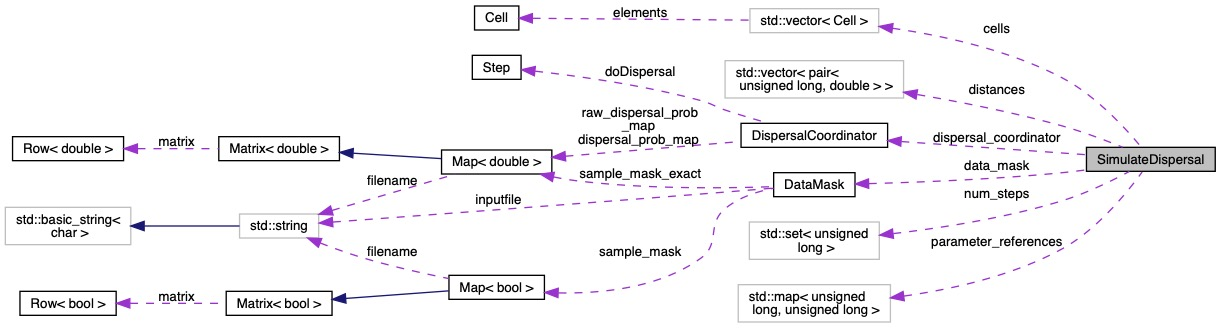
\includegraphics[width=350pt]{class_simulate_dispersal__coll__graph}
\end{center}
\end{figure}
\subsection*{Public Member Functions}
\begin{DoxyCompactItemize}
\item 
void \hyperlink{class_simulate_dispersal_a3da09319132db8c7ad035290be6590ef}{set\+Sequential} (bool b\+Sequential)
\begin{DoxyCompactList}\small\item\em Sets the is\+\_\+sequential flag. \end{DoxyCompactList}\item 
void \hyperlink{class_simulate_dispersal_ade30de5c9c7daebb6ccc4168fec3e813}{set\+Sizes} (unsigned long x, unsigned long y)
\begin{DoxyCompactList}\small\item\em Sets the sizes of the density map. \end{DoxyCompactList}\item 
void \hyperlink{class_simulate_dispersal_a8c7c65b4788010f02213fba5c985f49a}{import\+Maps} (string map\+\_\+file)
\begin{DoxyCompactList}\small\item\em Import the map from the prescribed file. \end{DoxyCompactList}\item 
void \hyperlink{class_simulate_dispersal_a46f2cd557ac9b21c107eac75e7c916af}{set\+Seed} (unsigned long s)
\begin{DoxyCompactList}\small\item\em Sets the seed for the random number generator. \end{DoxyCompactList}\item 
void \hyperlink{class_simulate_dispersal_a93b3d450679b00c015f5e18d91f3a426}{set\+Dispersal\+Parameters} (string dispersal\+\_\+method\+\_\+in, double sigma\+\_\+in, double tau\+\_\+in, double m\+\_\+prob\+\_\+in, double cutoff\+\_\+in, string landscape\+\_\+type)
\begin{DoxyCompactList}\small\item\em Sets the dispersal parameters. \end{DoxyCompactList}\item 
void {\bfseries set\+Landscape\+Type} (string landscape\+\_\+type)\hypertarget{class_simulate_dispersal_a627bcb0be7e7d6b0ef1dbd44b32a1909}{}\label{class_simulate_dispersal_a627bcb0be7e7d6b0ef1dbd44b32a1909}

\item 
void \hyperlink{class_simulate_dispersal_acae5067045d5989df6d7dce80bcfe276}{set\+Output\+Database} (string out\+\_\+database)
\begin{DoxyCompactList}\small\item\em Sets the output database for writing results to. \end{DoxyCompactList}\item 
void \hyperlink{class_simulate_dispersal_a29c7cf41d8b5610109d61f302fb32e73}{set\+Number\+Repeats} (unsigned long n)
\begin{DoxyCompactList}\small\item\em Sets the number of repeats to run the dispersal kernel for. \end{DoxyCompactList}\item 
void \hyperlink{class_simulate_dispersal_a4a38f61284426daa4d968bbab91d3608}{set\+Number\+Steps} (unsigned long s)
\begin{DoxyCompactList}\small\item\em Sets the number of steps to run each repeat of the dispersal kernel for when recording mean distance travelled. \end{DoxyCompactList}\item 
void \hyperlink{class_simulate_dispersal_a85d8ee68e5f4962429571c835aa028b4}{store\+Cell\+List} ()\hypertarget{class_simulate_dispersal_a85d8ee68e5f4962429571c835aa028b4}{}\label{class_simulate_dispersal_a85d8ee68e5f4962429571c835aa028b4}

\begin{DoxyCompactList}\small\item\em Calculates the list of cells to choose randomly from. \end{DoxyCompactList}\item 
const \hyperlink{struct_cell}{Cell} \& \hyperlink{class_simulate_dispersal_a7d0a2b28dd8d45f1b8a74dbcd82290e7}{get\+Random\+Cell} ()
\begin{DoxyCompactList}\small\item\em Gets a random cell from the list of cells. \end{DoxyCompactList}\item 
void \hyperlink{class_simulate_dispersal_a75eeedf1627eb25945a2d8f5dd0a2379}{calculate\+New\+Position} (const double \&dist, const double \&angle, const \hyperlink{struct_cell}{Cell} \&start\+\_\+cell, \hyperlink{struct_cell}{Cell} \&end\+\_\+cell)
\begin{DoxyCompactList}\small\item\em Calculates the new position from the start cell based on the distance and angle moved. Stores the new x and y location in the end cell. \end{DoxyCompactList}\item 
bool \hyperlink{class_simulate_dispersal_acb12b6b2f113e58c62636b2b4456f4da}{get\+End\+Point\+Infinite} (const double \&dist, const double \&angle, const \hyperlink{struct_cell}{Cell} \&this\+\_\+cell, \hyperlink{struct_cell}{Cell} \&end\+\_\+cell)
\begin{DoxyCompactList}\small\item\em Checks the density is greater than 0 a given distance from the start point on an infinite null landscape. \end{DoxyCompactList}\item 
bool \hyperlink{class_simulate_dispersal_a9694673493b261697020f42aa2fdf9e7}{get\+End\+Point\+Tiled} (const double \&dist, const double \&angle, const \hyperlink{struct_cell}{Cell} \&this\+\_\+cell, \hyperlink{struct_cell}{Cell} \&end\+\_\+cell)
\begin{DoxyCompactList}\small\item\em Checks the density is greater than 0 a given distance from the start point on an infinite tiled landscape. \end{DoxyCompactList}\item 
bool \hyperlink{class_simulate_dispersal_ab7fa3b37534cdd35871b30c7bb511351}{get\+End\+Point\+Closed} (const double \&dist, const double \&angle, const \hyperlink{struct_cell}{Cell} \&this\+\_\+cell, \hyperlink{struct_cell}{Cell} \&end\+\_\+cell)
\begin{DoxyCompactList}\small\item\em Checks the density a given distance from the start point on an closed landscape. \end{DoxyCompactList}\item 
bool \hyperlink{class_simulate_dispersal_a10a1dd769e993d018e7c7ae9208240ab}{get\+End\+Point} (const double \&dist, const double \&angle, const \hyperlink{struct_cell}{Cell} \&this\+\_\+cell, \hyperlink{struct_cell}{Cell} \&end\+\_\+cell)
\begin{DoxyCompactList}\small\item\em Checks the density a given distance from the start point, calling the relevant landscape function. \end{DoxyCompactList}\item 
void \hyperlink{class_simulate_dispersal_a4a759f6bb3b8288345eaf7c0d66ad29e}{run\+Mean\+Dispersal\+Distance} ()\hypertarget{class_simulate_dispersal_a4a759f6bb3b8288345eaf7c0d66ad29e}{}\label{class_simulate_dispersal_a4a759f6bb3b8288345eaf7c0d66ad29e}

\begin{DoxyCompactList}\small\item\em Simulates the dispersal kernel for the set parameters, storing the mean dispersal distance. \end{DoxyCompactList}\item 
void \hyperlink{class_simulate_dispersal_a406514e917874907cfb7a8d6c7889098}{run\+Mean\+Distance\+Travelled} ()\hypertarget{class_simulate_dispersal_a406514e917874907cfb7a8d6c7889098}{}\label{class_simulate_dispersal_a406514e917874907cfb7a8d6c7889098}

\begin{DoxyCompactList}\small\item\em Simulates the dispersal kernel for the set parameters, storing the mean distance travelled. \end{DoxyCompactList}\item 
void \hyperlink{class_simulate_dispersal_af7d0a726cb3724c159ca46f4586a8bd3}{write\+Database} (string table\+\_\+name)
\begin{DoxyCompactList}\small\item\em Writes out the distances to the S\+QL database. \end{DoxyCompactList}\item 
void \hyperlink{class_simulate_dispersal_ae0afed6eeb06f5bae4ee13a24850c8c5}{write\+Parameters} (string table\+\_\+name)
\begin{DoxyCompactList}\small\item\em Writes the simulation parameters to the output S\+QL database. \end{DoxyCompactList}\item 
void \hyperlink{class_simulate_dispersal_a0dee5d1529bd7ee6f382f7cd1b5393e5}{check\+Max\+Parameter\+Reference} ()\hypertarget{class_simulate_dispersal_a0dee5d1529bd7ee6f382f7cd1b5393e5}{}\label{class_simulate_dispersal_a0dee5d1529bd7ee6f382f7cd1b5393e5}

\begin{DoxyCompactList}\small\item\em Gets the maximum parameter reference from the output S\+QL database and saves val + 1 to parameter\+\_\+reference Assumes that the database exists. \end{DoxyCompactList}\item 
unsigned long \hyperlink{class_simulate_dispersal_abafd3fc30df157d12e462c4b1907d8fa}{check\+Max\+Id\+Number} (string table\+\_\+name)
\begin{DoxyCompactList}\small\item\em Gets the maximum id number from the output S\+QL database and returns val + 1 Assumes that the database exists. \end{DoxyCompactList}\end{DoxyCompactItemize}
\subsection*{Protected Types}
\begin{DoxyCompactItemize}
\item 
typedef bool(Simulate\+Dispersal\+::$\ast$ {\bfseries landscape\+\_\+fptr}) (const double \&dist, const double \&angle, const \hyperlink{struct_cell}{Cell} \&this\+\_\+cell, \hyperlink{struct_cell}{Cell} \&end\+\_\+cell)\hypertarget{class_simulate_dispersal_a33cf29f05f05fbf3cd70f759e62f57f0}{}\label{class_simulate_dispersal_a33cf29f05f05fbf3cd70f759e62f57f0}

\end{DoxyCompactItemize}
\subsection*{Protected Attributes}
\begin{DoxyCompactItemize}
\item 
\hyperlink{class_matrix}{Matrix}$<$ uint32\+\_\+t $>$ {\bfseries density\+\_\+map}\hypertarget{class_simulate_dispersal_aa699133749e7a30f225cb355f95f51e6}{}\label{class_simulate_dispersal_aa699133749e7a30f225cb355f95f51e6}

\item 
bool {\bfseries has\+\_\+set\+\_\+size}\hypertarget{class_simulate_dispersal_aff72c923e8454470b2d4c8935061fb21}{}\label{class_simulate_dispersal_aff72c923e8454470b2d4c8935061fb21}

\item 
\hyperlink{class_n_rrand}{N\+Rrand} {\bfseries random}\hypertarget{class_simulate_dispersal_a5f6389fc4116b52622a900c55532f86b}{}\label{class_simulate_dispersal_a5f6389fc4116b52622a900c55532f86b}

\item 
string {\bfseries map\+\_\+name}\hypertarget{class_simulate_dispersal_af1dc4cf60a69aafc2be4c80b0e9228c2}{}\label{class_simulate_dispersal_af1dc4cf60a69aafc2be4c80b0e9228c2}

\item 
unsigned long {\bfseries seed}\hypertarget{class_simulate_dispersal_af9ab2fa8b2c3e1bb1ba49b31679ae0d7}{}\label{class_simulate_dispersal_af9ab2fa8b2c3e1bb1ba49b31679ae0d7}

\item 
string {\bfseries dispersal\+\_\+method}\hypertarget{class_simulate_dispersal_aedabf3440f475bc15d4b95f9e8500d94}{}\label{class_simulate_dispersal_aedabf3440f475bc15d4b95f9e8500d94}

\item 
double {\bfseries sigma}\hypertarget{class_simulate_dispersal_ad6d6ae35911ed2bd045bf8e5bb30b628}{}\label{class_simulate_dispersal_ad6d6ae35911ed2bd045bf8e5bb30b628}

\item 
double {\bfseries tau}\hypertarget{class_simulate_dispersal_aa195b7e1b697c93e85a923eea5fabccc}{}\label{class_simulate_dispersal_aa195b7e1b697c93e85a923eea5fabccc}

\item 
double {\bfseries m\+\_\+prob}\hypertarget{class_simulate_dispersal_ae4b679b39467170abf45845d4591e6db}{}\label{class_simulate_dispersal_ae4b679b39467170abf45845d4591e6db}

\item 
double {\bfseries cutoff}\hypertarget{class_simulate_dispersal_a532f1c5ba22d681c5761dcce4fc8555d}{}\label{class_simulate_dispersal_a532f1c5ba22d681c5761dcce4fc8555d}

\item 
sqlite3 $\ast$ {\bfseries database}\hypertarget{class_simulate_dispersal_afd3f96f169715aacbcc2939614a6a910}{}\label{class_simulate_dispersal_afd3f96f169715aacbcc2939614a6a910}

\item 
vector$<$ double $>$ {\bfseries distances}\hypertarget{class_simulate_dispersal_a616354e9527a71396a428bb63f444a15}{}\label{class_simulate_dispersal_a616354e9527a71396a428bb63f444a15}

\item 
vector$<$ \hyperlink{struct_cell}{Cell} $>$ {\bfseries cells}\hypertarget{class_simulate_dispersal_abcb3ce61b835cbd007d09726302d692a}{}\label{class_simulate_dispersal_abcb3ce61b835cbd007d09726302d692a}

\item 
unsigned long {\bfseries num\+\_\+repeats}\hypertarget{class_simulate_dispersal_a36ca3df92a79e284cdeb84ea0dfb3c9a}{}\label{class_simulate_dispersal_a36ca3df92a79e284cdeb84ea0dfb3c9a}

\item 
unsigned long {\bfseries num\+\_\+steps}\hypertarget{class_simulate_dispersal_a7f3401f3a7f1ec48635973d94e3470e8}{}\label{class_simulate_dispersal_a7f3401f3a7f1ec48635973d94e3470e8}

\item 
unsigned long {\bfseries max\+\_\+density}\hypertarget{class_simulate_dispersal_a0edc9ca52d14b3ea78c99c33b200447e}{}\label{class_simulate_dispersal_a0edc9ca52d14b3ea78c99c33b200447e}

\item 
bool {\bfseries is\+\_\+sequential}\hypertarget{class_simulate_dispersal_a72f4b5ec8d52f080f2c9df991fb546ef}{}\label{class_simulate_dispersal_a72f4b5ec8d52f080f2c9df991fb546ef}

\item 
unsigned long {\bfseries parameter\+\_\+reference}\hypertarget{class_simulate_dispersal_a2d15ba06c50a249328f867a105848f72}{}\label{class_simulate_dispersal_a2d15ba06c50a249328f867a105848f72}

\item 
landscape\+\_\+fptr {\bfseries get\+Val\+Fptr}\hypertarget{class_simulate_dispersal_ae1f3a40b1805f024e41ec8df9c38c01e}{}\label{class_simulate_dispersal_ae1f3a40b1805f024e41ec8df9c38c01e}

\end{DoxyCompactItemize}


\subsection{Detailed Description}
Contains routines for importing a density map file, running a dispersal kernel n times on a landscape and record the dispersal distances. 

\subsection{Member Function Documentation}
\index{Simulate\+Dispersal@{Simulate\+Dispersal}!calculate\+New\+Position@{calculate\+New\+Position}}
\index{calculate\+New\+Position@{calculate\+New\+Position}!Simulate\+Dispersal@{Simulate\+Dispersal}}
\subsubsection[{\texorpdfstring{calculate\+New\+Position(const double \&dist, const double \&angle, const Cell \&start\+\_\+cell, Cell \&end\+\_\+cell)}{calculateNewPosition(const double &dist, const double &angle, const Cell &start_cell, Cell &end_cell)}}]{\setlength{\rightskip}{0pt plus 5cm}void Simulate\+Dispersal\+::calculate\+New\+Position (
\begin{DoxyParamCaption}
\item[{const double \&}]{dist, }
\item[{const double \&}]{angle, }
\item[{const {\bf Cell} \&}]{start\+\_\+cell, }
\item[{{\bf Cell} \&}]{end\+\_\+cell}
\end{DoxyParamCaption}
)}\hypertarget{class_simulate_dispersal_a75eeedf1627eb25945a2d8f5dd0a2379}{}\label{class_simulate_dispersal_a75eeedf1627eb25945a2d8f5dd0a2379}


Calculates the new position from the start cell based on the distance and angle moved. Stores the new x and y location in the end cell. 


\begin{DoxyParams}{Parameters}
{\em dist} & the distance to move \\
\hline
{\em angle} & the direction from the start cell to move \\
\hline
{\em start\+\_\+cell} & the cell containing the start x and y position \\
\hline
{\em end\+\_\+cell} & the cell to contain the end x and y position \\
\hline
\end{DoxyParams}
\index{Simulate\+Dispersal@{Simulate\+Dispersal}!check\+Max\+Id\+Number@{check\+Max\+Id\+Number}}
\index{check\+Max\+Id\+Number@{check\+Max\+Id\+Number}!Simulate\+Dispersal@{Simulate\+Dispersal}}
\subsubsection[{\texorpdfstring{check\+Max\+Id\+Number(string table\+\_\+name)}{checkMaxIdNumber(string table_name)}}]{\setlength{\rightskip}{0pt plus 5cm}unsigned long Simulate\+Dispersal\+::check\+Max\+Id\+Number (
\begin{DoxyParamCaption}
\item[{string}]{table\+\_\+name}
\end{DoxyParamCaption}
)}\hypertarget{class_simulate_dispersal_abafd3fc30df157d12e462c4b1907d8fa}{}\label{class_simulate_dispersal_abafd3fc30df157d12e462c4b1907d8fa}


Gets the maximum id number from the output S\+QL database and returns val + 1 Assumes that the database exists. 

\begin{DoxyNote}{Note}
this function does not check for S\+QL injection attacks and should not be used with variable function names. 
\end{DoxyNote}

\begin{DoxyParams}{Parameters}
{\em table\+\_\+name} & the name of the table to check for max(id) in \\
\hline
\end{DoxyParams}
\begin{DoxyReturn}{Returns}
the maximum id + 1 from the given table 
\end{DoxyReturn}
\index{Simulate\+Dispersal@{Simulate\+Dispersal}!get\+End\+Point@{get\+End\+Point}}
\index{get\+End\+Point@{get\+End\+Point}!Simulate\+Dispersal@{Simulate\+Dispersal}}
\subsubsection[{\texorpdfstring{get\+End\+Point(const double \&dist, const double \&angle, const Cell \&this\+\_\+cell, Cell \&end\+\_\+cell)}{getEndPoint(const double &dist, const double &angle, const Cell &this_cell, Cell &end_cell)}}]{\setlength{\rightskip}{0pt plus 5cm}bool Simulate\+Dispersal\+::get\+End\+Point (
\begin{DoxyParamCaption}
\item[{const double \&}]{dist, }
\item[{const double \&}]{angle, }
\item[{const {\bf Cell} \&}]{this\+\_\+cell, }
\item[{{\bf Cell} \&}]{end\+\_\+cell}
\end{DoxyParamCaption}
)}\hypertarget{class_simulate_dispersal_a10a1dd769e993d018e7c7ae9208240ab}{}\label{class_simulate_dispersal_a10a1dd769e993d018e7c7ae9208240ab}


Checks the density a given distance from the start point, calling the relevant landscape function. 

This also takes into account the rejection sampling of density based on the maximal density value from the map.


\begin{DoxyParams}{Parameters}
{\em dist} & the distance of dispersal \\
\hline
{\em angle} & the angle of dispersal \\
\hline
{\em this\+\_\+cell} & \hyperlink{struct_cell}{Cell} containing the x and y coordinates of the starting position \\
\hline
{\em end\+\_\+cell} & \hyperlink{struct_cell}{Cell} to store the end point in\\
\hline
\end{DoxyParams}
\begin{DoxyReturn}{Returns}
true if the point has a density $>$ 0, otherwise generates a random number between 0 and the max size and if it is $>$ the density, return true, false otherwise. 
\end{DoxyReturn}
\index{Simulate\+Dispersal@{Simulate\+Dispersal}!get\+End\+Point\+Closed@{get\+End\+Point\+Closed}}
\index{get\+End\+Point\+Closed@{get\+End\+Point\+Closed}!Simulate\+Dispersal@{Simulate\+Dispersal}}
\subsubsection[{\texorpdfstring{get\+End\+Point\+Closed(const double \&dist, const double \&angle, const Cell \&this\+\_\+cell, Cell \&end\+\_\+cell)}{getEndPointClosed(const double &dist, const double &angle, const Cell &this_cell, Cell &end_cell)}}]{\setlength{\rightskip}{0pt plus 5cm}bool Simulate\+Dispersal\+::get\+End\+Point\+Closed (
\begin{DoxyParamCaption}
\item[{const double \&}]{dist, }
\item[{const double \&}]{angle, }
\item[{const {\bf Cell} \&}]{this\+\_\+cell, }
\item[{{\bf Cell} \&}]{end\+\_\+cell}
\end{DoxyParamCaption}
)}\hypertarget{class_simulate_dispersal_ab7fa3b37534cdd35871b30c7bb511351}{}\label{class_simulate_dispersal_ab7fa3b37534cdd35871b30c7bb511351}


Checks the density a given distance from the start point on an closed landscape. 

This also takes into account the rejection sampling of density based on the maximal density value from the map.


\begin{DoxyParams}{Parameters}
{\em dist} & the distance of dispersal \\
\hline
{\em angle} & the angle of dispersal \\
\hline
{\em this\+\_\+cell} & \hyperlink{struct_cell}{Cell} containing the x and y coordinates of the starting position \\
\hline
{\em end\+\_\+cell} & \hyperlink{struct_cell}{Cell} to store the end point in\\
\hline
\end{DoxyParams}
\begin{DoxyReturn}{Returns}
true if the point has a density $>$ 0, otherwise generates a random number between 0 and the max size and if it is $>$ the density, return true, false otherwise. 
\end{DoxyReturn}
\index{Simulate\+Dispersal@{Simulate\+Dispersal}!get\+End\+Point\+Infinite@{get\+End\+Point\+Infinite}}
\index{get\+End\+Point\+Infinite@{get\+End\+Point\+Infinite}!Simulate\+Dispersal@{Simulate\+Dispersal}}
\subsubsection[{\texorpdfstring{get\+End\+Point\+Infinite(const double \&dist, const double \&angle, const Cell \&this\+\_\+cell, Cell \&end\+\_\+cell)}{getEndPointInfinite(const double &dist, const double &angle, const Cell &this_cell, Cell &end_cell)}}]{\setlength{\rightskip}{0pt plus 5cm}bool Simulate\+Dispersal\+::get\+End\+Point\+Infinite (
\begin{DoxyParamCaption}
\item[{const double \&}]{dist, }
\item[{const double \&}]{angle, }
\item[{const {\bf Cell} \&}]{this\+\_\+cell, }
\item[{{\bf Cell} \&}]{end\+\_\+cell}
\end{DoxyParamCaption}
)}\hypertarget{class_simulate_dispersal_acb12b6b2f113e58c62636b2b4456f4da}{}\label{class_simulate_dispersal_acb12b6b2f113e58c62636b2b4456f4da}


Checks the density is greater than 0 a given distance from the start point on an infinite null landscape. 

This also takes into account the rejection sampling of density based on the maximal density value from the map.


\begin{DoxyParams}{Parameters}
{\em dist} & the distance of dispersal \\
\hline
{\em angle} & the angle of dispersal \\
\hline
{\em this\+\_\+cell} & \hyperlink{struct_cell}{Cell} containing the x and y coordinates of the starting position \\
\hline
{\em end\+\_\+cell} & \hyperlink{struct_cell}{Cell} to store the end point in \\
\hline
\end{DoxyParams}
\begin{DoxyReturn}{Returns}
true if the point has a density $>$ 0, otherwise generates a random number between 0 and the max size and if it is $>$ the density, return true, false otherwise. 
\end{DoxyReturn}
\index{Simulate\+Dispersal@{Simulate\+Dispersal}!get\+End\+Point\+Tiled@{get\+End\+Point\+Tiled}}
\index{get\+End\+Point\+Tiled@{get\+End\+Point\+Tiled}!Simulate\+Dispersal@{Simulate\+Dispersal}}
\subsubsection[{\texorpdfstring{get\+End\+Point\+Tiled(const double \&dist, const double \&angle, const Cell \&this\+\_\+cell, Cell \&end\+\_\+cell)}{getEndPointTiled(const double &dist, const double &angle, const Cell &this_cell, Cell &end_cell)}}]{\setlength{\rightskip}{0pt plus 5cm}bool Simulate\+Dispersal\+::get\+End\+Point\+Tiled (
\begin{DoxyParamCaption}
\item[{const double \&}]{dist, }
\item[{const double \&}]{angle, }
\item[{const {\bf Cell} \&}]{this\+\_\+cell, }
\item[{{\bf Cell} \&}]{end\+\_\+cell}
\end{DoxyParamCaption}
)}\hypertarget{class_simulate_dispersal_a9694673493b261697020f42aa2fdf9e7}{}\label{class_simulate_dispersal_a9694673493b261697020f42aa2fdf9e7}


Checks the density is greater than 0 a given distance from the start point on an infinite tiled landscape. 

This also takes into account the rejection sampling of density based on the maximal density value from the map.


\begin{DoxyParams}{Parameters}
{\em dist} & the distance of dispersal \\
\hline
{\em angle} & the angle of dispersal \\
\hline
{\em this\+\_\+cell} & \hyperlink{struct_cell}{Cell} containing the x and y coordinates of the starting position \\
\hline
{\em end\+\_\+cell} & \hyperlink{struct_cell}{Cell} to store the end point in\\
\hline
\end{DoxyParams}
\begin{DoxyReturn}{Returns}
true if the point has a density $>$ 0, otherwise generates a random number between 0 and the max size and if it is $>$ the density, return true, false otherwise. 
\end{DoxyReturn}
\index{Simulate\+Dispersal@{Simulate\+Dispersal}!get\+Random\+Cell@{get\+Random\+Cell}}
\index{get\+Random\+Cell@{get\+Random\+Cell}!Simulate\+Dispersal@{Simulate\+Dispersal}}
\subsubsection[{\texorpdfstring{get\+Random\+Cell()}{getRandomCell()}}]{\setlength{\rightskip}{0pt plus 5cm}const {\bf Cell} \& Simulate\+Dispersal\+::get\+Random\+Cell (
\begin{DoxyParamCaption}
{}
\end{DoxyParamCaption}
)}\hypertarget{class_simulate_dispersal_a7d0a2b28dd8d45f1b8a74dbcd82290e7}{}\label{class_simulate_dispersal_a7d0a2b28dd8d45f1b8a74dbcd82290e7}


Gets a random cell from the list of cells. 

\begin{DoxyReturn}{Returns}
a \hyperlink{struct_cell}{Cell} object reference containing the x and y positions to choose from 
\end{DoxyReturn}
\index{Simulate\+Dispersal@{Simulate\+Dispersal}!import\+Maps@{import\+Maps}}
\index{import\+Maps@{import\+Maps}!Simulate\+Dispersal@{Simulate\+Dispersal}}
\subsubsection[{\texorpdfstring{import\+Maps(string map\+\_\+file)}{importMaps(string map_file)}}]{\setlength{\rightskip}{0pt plus 5cm}void Simulate\+Dispersal\+::import\+Maps (
\begin{DoxyParamCaption}
\item[{string}]{map\+\_\+file}
\end{DoxyParamCaption}
)}\hypertarget{class_simulate_dispersal_a8c7c65b4788010f02213fba5c985f49a}{}\label{class_simulate_dispersal_a8c7c65b4788010f02213fba5c985f49a}


Import the map from the prescribed file. 


\begin{DoxyParams}{Parameters}
{\em map\+\_\+file} & the map file to import from \\
\hline
\end{DoxyParams}
\index{Simulate\+Dispersal@{Simulate\+Dispersal}!set\+Dispersal\+Parameters@{set\+Dispersal\+Parameters}}
\index{set\+Dispersal\+Parameters@{set\+Dispersal\+Parameters}!Simulate\+Dispersal@{Simulate\+Dispersal}}
\subsubsection[{\texorpdfstring{set\+Dispersal\+Parameters(string dispersal\+\_\+method\+\_\+in, double sigma\+\_\+in, double tau\+\_\+in, double m\+\_\+prob\+\_\+in, double cutoff\+\_\+in, string landscape\+\_\+type)}{setDispersalParameters(string dispersal_method_in, double sigma_in, double tau_in, double m_prob_in, double cutoff_in, string landscape_type)}}]{\setlength{\rightskip}{0pt plus 5cm}void Simulate\+Dispersal\+::set\+Dispersal\+Parameters (
\begin{DoxyParamCaption}
\item[{string}]{dispersal\+\_\+method\+\_\+in, }
\item[{double}]{sigma\+\_\+in, }
\item[{double}]{tau\+\_\+in, }
\item[{double}]{m\+\_\+prob\+\_\+in, }
\item[{double}]{cutoff\+\_\+in, }
\item[{string}]{landscape\+\_\+type}
\end{DoxyParamCaption}
)}\hypertarget{class_simulate_dispersal_a93b3d450679b00c015f5e18d91f3a426}{}\label{class_simulate_dispersal_a93b3d450679b00c015f5e18d91f3a426}


Sets the dispersal parameters. 


\begin{DoxyParams}{Parameters}
{\em dispersal\+\_\+method\+\_\+in} & the dispersal method (e.\+g. \char`\"{}normal\char`\"{}) \\
\hline
{\em sigma\+\_\+in} & the sigma value for normal and fat-\/tailed dispersals \\
\hline
{\em tau\+\_\+in} & the nu value for fat-\/tailed dispersals \\
\hline
{\em m\+\_\+prob\+\_\+in} & the m\+\_\+prob for norm-\/uniform dispersals \\
\hline
{\em cutoff\+\_\+in} & the maximum dispersal distance for norm-\/uniform dispersal \\
\hline
{\em landscape\+\_\+type} & string containing the landscape type (one of \char`\"{}closed\char`\"{}, \char`\"{}tiled\char`\"{} or \char`\"{}infinite\char`\"{}). \\
\hline
\end{DoxyParams}
\index{Simulate\+Dispersal@{Simulate\+Dispersal}!set\+Number\+Repeats@{set\+Number\+Repeats}}
\index{set\+Number\+Repeats@{set\+Number\+Repeats}!Simulate\+Dispersal@{Simulate\+Dispersal}}
\subsubsection[{\texorpdfstring{set\+Number\+Repeats(unsigned long n)}{setNumberRepeats(unsigned long n)}}]{\setlength{\rightskip}{0pt plus 5cm}void Simulate\+Dispersal\+::set\+Number\+Repeats (
\begin{DoxyParamCaption}
\item[{unsigned long}]{n}
\end{DoxyParamCaption}
)}\hypertarget{class_simulate_dispersal_a29c7cf41d8b5610109d61f302fb32e73}{}\label{class_simulate_dispersal_a29c7cf41d8b5610109d61f302fb32e73}


Sets the number of repeats to run the dispersal kernel for. 


\begin{DoxyParams}{Parameters}
{\em n} & the number of repeats \\
\hline
\end{DoxyParams}
\index{Simulate\+Dispersal@{Simulate\+Dispersal}!set\+Number\+Steps@{set\+Number\+Steps}}
\index{set\+Number\+Steps@{set\+Number\+Steps}!Simulate\+Dispersal@{Simulate\+Dispersal}}
\subsubsection[{\texorpdfstring{set\+Number\+Steps(unsigned long s)}{setNumberSteps(unsigned long s)}}]{\setlength{\rightskip}{0pt plus 5cm}void Simulate\+Dispersal\+::set\+Number\+Steps (
\begin{DoxyParamCaption}
\item[{unsigned long}]{s}
\end{DoxyParamCaption}
)}\hypertarget{class_simulate_dispersal_a4a38f61284426daa4d968bbab91d3608}{}\label{class_simulate_dispersal_a4a38f61284426daa4d968bbab91d3608}


Sets the number of steps to run each repeat of the dispersal kernel for when recording mean distance travelled. 


\begin{DoxyParams}{Parameters}
{\em s} & the number of steps \\
\hline
\end{DoxyParams}
\index{Simulate\+Dispersal@{Simulate\+Dispersal}!set\+Output\+Database@{set\+Output\+Database}}
\index{set\+Output\+Database@{set\+Output\+Database}!Simulate\+Dispersal@{Simulate\+Dispersal}}
\subsubsection[{\texorpdfstring{set\+Output\+Database(string out\+\_\+database)}{setOutputDatabase(string out_database)}}]{\setlength{\rightskip}{0pt plus 5cm}void Simulate\+Dispersal\+::set\+Output\+Database (
\begin{DoxyParamCaption}
\item[{string}]{out\+\_\+database}
\end{DoxyParamCaption}
)}\hypertarget{class_simulate_dispersal_acae5067045d5989df6d7dce80bcfe276}{}\label{class_simulate_dispersal_acae5067045d5989df6d7dce80bcfe276}


Sets the output database for writing results to. 


\begin{DoxyParams}{Parameters}
{\em out\+\_\+database} & path to the output database \\
\hline
\end{DoxyParams}
\index{Simulate\+Dispersal@{Simulate\+Dispersal}!set\+Seed@{set\+Seed}}
\index{set\+Seed@{set\+Seed}!Simulate\+Dispersal@{Simulate\+Dispersal}}
\subsubsection[{\texorpdfstring{set\+Seed(unsigned long s)}{setSeed(unsigned long s)}}]{\setlength{\rightskip}{0pt plus 5cm}void Simulate\+Dispersal\+::set\+Seed (
\begin{DoxyParamCaption}
\item[{unsigned long}]{s}
\end{DoxyParamCaption}
)\hspace{0.3cm}{\ttfamily [inline]}}\hypertarget{class_simulate_dispersal_a46f2cd557ac9b21c107eac75e7c916af}{}\label{class_simulate_dispersal_a46f2cd557ac9b21c107eac75e7c916af}


Sets the seed for the random number generator. 


\begin{DoxyParams}{Parameters}
{\em s} & the seed \\
\hline
\end{DoxyParams}
\index{Simulate\+Dispersal@{Simulate\+Dispersal}!set\+Sequential@{set\+Sequential}}
\index{set\+Sequential@{set\+Sequential}!Simulate\+Dispersal@{Simulate\+Dispersal}}
\subsubsection[{\texorpdfstring{set\+Sequential(bool b\+Sequential)}{setSequential(bool bSequential)}}]{\setlength{\rightskip}{0pt plus 5cm}void Simulate\+Dispersal\+::set\+Sequential (
\begin{DoxyParamCaption}
\item[{bool}]{b\+Sequential}
\end{DoxyParamCaption}
)}\hypertarget{class_simulate_dispersal_a3da09319132db8c7ad035290be6590ef}{}\label{class_simulate_dispersal_a3da09319132db8c7ad035290be6590ef}


Sets the is\+\_\+sequential flag. 


\begin{DoxyParams}{Parameters}
{\em b\+Sequential} & if true, dispersal events are selected using the end point of the last dispersal distance for the start of the next move event \\
\hline
\end{DoxyParams}
\index{Simulate\+Dispersal@{Simulate\+Dispersal}!set\+Sizes@{set\+Sizes}}
\index{set\+Sizes@{set\+Sizes}!Simulate\+Dispersal@{Simulate\+Dispersal}}
\subsubsection[{\texorpdfstring{set\+Sizes(unsigned long x, unsigned long y)}{setSizes(unsigned long x, unsigned long y)}}]{\setlength{\rightskip}{0pt plus 5cm}void Simulate\+Dispersal\+::set\+Sizes (
\begin{DoxyParamCaption}
\item[{unsigned long}]{x, }
\item[{unsigned long}]{y}
\end{DoxyParamCaption}
)}\hypertarget{class_simulate_dispersal_ade30de5c9c7daebb6ccc4168fec3e813}{}\label{class_simulate_dispersal_ade30de5c9c7daebb6ccc4168fec3e813}


Sets the sizes of the density map. 


\begin{DoxyParams}{Parameters}
{\em x} & the x dimension (number of columns) in the density map \\
\hline
{\em y} & the y dimension (number of rows) in the density map \\
\hline
\end{DoxyParams}
\index{Simulate\+Dispersal@{Simulate\+Dispersal}!write\+Database@{write\+Database}}
\index{write\+Database@{write\+Database}!Simulate\+Dispersal@{Simulate\+Dispersal}}
\subsubsection[{\texorpdfstring{write\+Database(string table\+\_\+name)}{writeDatabase(string table_name)}}]{\setlength{\rightskip}{0pt plus 5cm}void Simulate\+Dispersal\+::write\+Database (
\begin{DoxyParamCaption}
\item[{string}]{table\+\_\+name}
\end{DoxyParamCaption}
)}\hypertarget{class_simulate_dispersal_af7d0a726cb3724c159ca46f4586a8bd3}{}\label{class_simulate_dispersal_af7d0a726cb3724c159ca46f4586a8bd3}


Writes out the distances to the S\+QL database. 


\begin{DoxyParams}{Parameters}
{\em table\+\_\+name} & the name of the table to output to, either \textquotesingle{}D\+I\+S\+P\+E\+R\+S\+A\+L\+\_\+\+D\+I\+S\+T\+A\+N\+CE\textquotesingle{} or \textquotesingle{}D\+I\+S\+T\+A\+N\+C\+E\+S\+\_\+\+T\+R\+A\+V\+E\+L\+L\+ED\textquotesingle{} \\
\hline
\end{DoxyParams}
\index{Simulate\+Dispersal@{Simulate\+Dispersal}!write\+Parameters@{write\+Parameters}}
\index{write\+Parameters@{write\+Parameters}!Simulate\+Dispersal@{Simulate\+Dispersal}}
\subsubsection[{\texorpdfstring{write\+Parameters(string table\+\_\+name)}{writeParameters(string table_name)}}]{\setlength{\rightskip}{0pt plus 5cm}void Simulate\+Dispersal\+::write\+Parameters (
\begin{DoxyParamCaption}
\item[{string}]{table\+\_\+name}
\end{DoxyParamCaption}
)}\hypertarget{class_simulate_dispersal_ae0afed6eeb06f5bae4ee13a24850c8c5}{}\label{class_simulate_dispersal_ae0afed6eeb06f5bae4ee13a24850c8c5}


Writes the simulation parameters to the output S\+QL database. 


\begin{DoxyParams}{Parameters}
{\em table\+\_\+name} & the name of the table to output to, either \textquotesingle{}D\+I\+S\+P\+E\+R\+S\+A\+L\+\_\+\+D\+I\+S\+T\+A\+N\+CE\textquotesingle{} or \textquotesingle{}D\+I\+S\+T\+A\+N\+C\+E\+S\+\_\+\+T\+R\+A\+V\+E\+L\+L\+ED\textquotesingle{} \\
\hline
\end{DoxyParams}


The documentation for this class was generated from the following files\+:\begin{DoxyCompactItemize}
\item 
necsim/\hyperlink{_simulate_dispersal_8h}{Simulate\+Dispersal.\+h}\item 
necsim/\hyperlink{_simulate_dispersal_8cpp}{Simulate\+Dispersal.\+cpp}\end{DoxyCompactItemize}

\hypertarget{struct_species_exception}{}\section{Species\+Exception Struct Reference}
\label{struct_species_exception}\index{Species\+Exception@{Species\+Exception}}


An exception thrown whenever a non-\/fatal Species exception is thrown.  




{\ttfamily \#include $<$Custom\+Exceptions.\+h$>$}



Inheritance diagram for Species\+Exception\+:
% FIG 0


Collaboration diagram for Species\+Exception\+:
% FIG 1
\subsection*{Public Member Functions}
\begin{DoxyCompactItemize}
\item 
\hyperlink{struct_species_exception_aad9febae65922d3a68a3d70ddc8b6a16}{Species\+Exception} ()\hypertarget{struct_species_exception_aad9febae65922d3a68a3d70ddc8b6a16}{}\label{struct_species_exception_aad9febae65922d3a68a3d70ddc8b6a16}

\begin{DoxyCompactList}\small\item\em Throws a runtime\+\_\+error with a custom message indicating source. \end{DoxyCompactList}\item 
\hyperlink{struct_species_exception_aee4c223dc1b702be3b937556f39b26a5}{Species\+Exception} (string msg)
\begin{DoxyCompactList}\small\item\em Overloaded runtime\+\_\+error call which provides error message parsing. \end{DoxyCompactList}\end{DoxyCompactItemize}


\subsection{Detailed Description}
An exception thrown whenever a non-\/fatal Species exception is thrown. 

\subsection{Constructor \& Destructor Documentation}
\index{Species\+Exception@{Species\+Exception}!Species\+Exception@{Species\+Exception}}
\index{Species\+Exception@{Species\+Exception}!Species\+Exception@{Species\+Exception}}
\subsubsection[{\texorpdfstring{Species\+Exception(string msg)}{SpeciesException(string msg)}}]{\setlength{\rightskip}{0pt plus 5cm}Species\+Exception\+::\+Species\+Exception (
\begin{DoxyParamCaption}
\item[{string}]{msg}
\end{DoxyParamCaption}
)\hspace{0.3cm}{\ttfamily [inline]}}\hypertarget{struct_species_exception_aee4c223dc1b702be3b937556f39b26a5}{}\label{struct_species_exception_aee4c223dc1b702be3b937556f39b26a5}


Overloaded runtime\+\_\+error call which provides error message parsing. 


\begin{DoxyParams}{Parameters}
{\em msg} & the message to be passed to the runtime\+\_\+error \\
\hline
\end{DoxyParams}


The documentation for this struct was generated from the following file\+:\begin{DoxyCompactItemize}
\item 
\hyperlink{_custom_exceptions_8h}{Custom\+Exceptions.\+h}\end{DoxyCompactItemize}

\hypertarget{class_species_list}{}\section{Species\+List Class Reference}
\label{class_species_list}\index{Species\+List@{Species\+List}}


Contains a list of the species that exist at one location. The \hyperlink{class_row}{Row} object, list, contains the active reference number, for looking up the lineage in a \hyperlink{class_row}{Row} of Datapoint objects. Also contains the functions for correctly generating coalescence probabilities and list management.  




{\ttfamily \#include $<$Species\+List.\+h$>$}

\subsection*{Public Member Functions}
\begin{DoxyCompactItemize}
\item 
\hyperlink{class_species_list_a5ebcb2cf12fc4e7a3d8bbd650814a5fb}{Species\+List} ()\hypertarget{class_species_list_a5ebcb2cf12fc4e7a3d8bbd650814a5fb}{}\label{class_species_list_a5ebcb2cf12fc4e7a3d8bbd650814a5fb}

\begin{DoxyCompactList}\small\item\em Default constructor. \end{DoxyCompactList}\item 
\hyperlink{class_species_list_a16e2d58a8643fa58eb25e8258682965c}{$\sim$\+Species\+List} ()=default\hypertarget{class_species_list_a16e2d58a8643fa58eb25e8258682965c}{}\label{class_species_list_a16e2d58a8643fa58eb25e8258682965c}

\begin{DoxyCompactList}\small\item\em Default destructor. \end{DoxyCompactList}\item 
void \hyperlink{class_species_list_ad617317047f221e64066dd851b9e8d2d}{fill\+List} ()\hypertarget{class_species_list_ad617317047f221e64066dd851b9e8d2d}{}\label{class_species_list_ad617317047f221e64066dd851b9e8d2d}

\begin{DoxyCompactList}\small\item\em Fills the list with 0, up to the specified maximum size. \end{DoxyCompactList}\item 
void \hyperlink{class_species_list_ab36fdc058217514e66e6152479dfab8d}{initialise} (unsigned long maxsizein)
\begin{DoxyCompactList}\small\item\em Initialises the list to the specified size. \end{DoxyCompactList}\item 
void \hyperlink{class_species_list_a8532bddc8397cf50531639c50cccbef3}{set\+Maxsize} (unsigned long maxsizein)
\begin{DoxyCompactList}\small\item\em Sets the maxsize without altering the actual size of list. \end{DoxyCompactList}\item 
void \hyperlink{class_species_list_a98f19fa65ed7cbe4536342ce2dff2b7b}{set\+Species} (unsigned long index, unsigned long new\+\_\+val)
\begin{DoxyCompactList}\small\item\em Set specific entry to a particular species reference number. \end{DoxyCompactList}\item 
void \hyperlink{class_species_list_ae4b1baaacea721479c8585d36b475c96}{set\+Species\+Empty} (int index, unsigned long new\+\_\+val)
\begin{DoxyCompactList}\small\item\em Set specific entry to a particular species reference number. \end{DoxyCompactList}\item 
void \hyperlink{class_species_list_a627f9d95948f4a2cb6cfb3d8b8f9f2ea}{set\+Next} (unsigned long n)
\begin{DoxyCompactList}\small\item\em Set the next active lineage (for wrapping purposes). \end{DoxyCompactList}\item 
void \hyperlink{class_species_list_ad3f8f91e3983b8829c0b405013b2709e}{set\+Nwrap} (unsigned long nr)
\begin{DoxyCompactList}\small\item\em Set the number of wrapping lineages. \end{DoxyCompactList}\item 
unsigned long \hyperlink{class_species_list_a4a54fa9e6c07f8d75d9cddbf9a04da19}{add\+Species} (unsigned long new\+\_\+spec)
\begin{DoxyCompactList}\small\item\em Add a new species to the first empty place and return the position of the lineage. \end{DoxyCompactList}\item 
void \hyperlink{class_species_list_af84a5aa6584f16dfb8e8f2ce379cf947}{add\+Species\+Silent} (unsigned long new\+\_\+spec)
\begin{DoxyCompactList}\small\item\em Add a new species to the first empty place. Essentially a version of \hyperlink{class_species_list_a4a54fa9e6c07f8d75d9cddbf9a04da19}{add\+Species()} without returning the species location. \end{DoxyCompactList}\item 
void \hyperlink{class_species_list_af7464b3a3ea20220634ab38476a195e4}{delete\+Species} (unsigned long index)
\begin{DoxyCompactList}\small\item\em Removes the species at the specified index. The species number will be replaced with 0, indicating no species present. \end{DoxyCompactList}\item 
void \hyperlink{class_species_list_a15420717ab0ba00bba0ff55f971ee3d2}{decrease\+Nwrap} ()
\begin{DoxyCompactList}\small\item\em Decreases the nwrap by one. \end{DoxyCompactList}\item 
void \hyperlink{class_species_list_ac15ecbcddcce068f75162dac03eafcfc}{increase\+List\+Size} ()\hypertarget{class_species_list_ac15ecbcddcce068f75162dac03eafcfc}{}\label{class_species_list_ac15ecbcddcce068f75162dac03eafcfc}

\begin{DoxyCompactList}\small\item\em Increases the list size by one. \end{DoxyCompactList}\item 
void \hyperlink{class_species_list_aa9e64b4e922b43c17e188ca2038cb18a}{increase\+Nwrap} ()
\begin{DoxyCompactList}\small\item\em Increases the nwrap by one. \end{DoxyCompactList}\item 
void \hyperlink{class_species_list_a40206bc9836f394653997a61c1c8617a}{change\+Percent\+Cover} (unsigned long newmaxsize)
\begin{DoxyCompactList}\small\item\em Changes the maximum size of the \hyperlink{class_species_list}{Species\+List}. Creates a new list object with all the species in the correct place from the old list object and zeros everywhere else. \end{DoxyCompactList}\item 
unsigned long \hyperlink{class_species_list_a8e57aa257510bf61680e53c548fd4610}{get\+Rand\+Lineage} (\hyperlink{class_n_rrand}{N\+Rrand} \&rand\+\_\+no)
\begin{DoxyCompactList}\small\item\em Get a random species reference number from all the potential entries. Updated alternative version returns any entry, including empty cells, giving the probability of coalescence as well. \end{DoxyCompactList}\item 
unsigned long \hyperlink{class_species_list_ab215c2790feb1a721c759bbb1c434f85}{get\+Species} (unsigned long index)
\begin{DoxyCompactList}\small\item\em Get the species reference number from a particular entry. \end{DoxyCompactList}\item 
unsigned long \hyperlink{class_species_list_ac3fffc2d47557af6964cb25336d0e5cc}{get\+Next} ()
\begin{DoxyCompactList}\small\item\em Get the next\+\_\+active variable. \end{DoxyCompactList}\item 
unsigned long \hyperlink{class_species_list_a9cd0acb0d22d6b14c4d58668cdb36af3}{get\+Nwrap} ()
\begin{DoxyCompactList}\small\item\em Getter for the nwrap. \end{DoxyCompactList}\item 
unsigned long \hyperlink{class_species_list_a9c6206262b57a450eb92c95f94bd59f7}{get\+Listsize} ()
\begin{DoxyCompactList}\small\item\em Getter for the list size. \end{DoxyCompactList}\item 
unsigned long \hyperlink{class_species_list_ad7d1f16709df32455743995ecb61ed9e}{get\+Maxsize} ()
\begin{DoxyCompactList}\small\item\em Getter for the maximum size of the \hyperlink{class_species_list}{Species\+List} object. \end{DoxyCompactList}\item 
void \hyperlink{class_species_list_acd0fd4ab7517523f04d8c37bb918d390}{wipe\+List} ()\hypertarget{class_species_list_acd0fd4ab7517523f04d8c37bb918d390}{}\label{class_species_list_acd0fd4ab7517523f04d8c37bb918d390}

\begin{DoxyCompactList}\small\item\em Empties the list of any data and fills the list with zeros. \end{DoxyCompactList}\end{DoxyCompactItemize}
\subsection*{Friends}
\begin{DoxyCompactItemize}
\item 
ostream \& \hyperlink{class_species_list_a307fffef634cd0a4615794ef7498cd4a}{operator$<$$<$} (ostream \&os, const \hyperlink{class_species_list}{Species\+List} \&r)
\begin{DoxyCompactList}\small\item\em Outputs the \hyperlink{class_species_list}{Species\+List} object to an output stream. Allows for piping to the terminal or writing the object to a file. \end{DoxyCompactList}\item 
istream \& \hyperlink{class_species_list_a2d74faa6012ce148a9f437249390c294}{operator$>$$>$} (istream \&is, \hyperlink{class_species_list}{Species\+List} \&r)
\begin{DoxyCompactList}\small\item\em Inputs the \hyperlink{class_species_list}{Species\+List} object from an input stream. Allows for reading data from a file or string stream. \end{DoxyCompactList}\end{DoxyCompactItemize}


\subsection{Detailed Description}
Contains a list of the species that exist at one location. The \hyperlink{class_row}{Row} object, list, contains the active reference number, for looking up the lineage in a \hyperlink{class_row}{Row} of Datapoint objects. Also contains the functions for correctly generating coalescence probabilities and list management. 

Note that the maximum size of the list is constrained by the maximum size of unsigned long. Any simulation requiring more individuals per cell than this will unlikely finish in any reasonable time anyway. 

\subsection{Member Function Documentation}
\index{Species\+List@{Species\+List}!add\+Species@{add\+Species}}
\index{add\+Species@{add\+Species}!Species\+List@{Species\+List}}
\subsubsection[{\texorpdfstring{add\+Species(unsigned long new\+\_\+spec)}{addSpecies(unsigned long new_spec)}}]{\setlength{\rightskip}{0pt plus 5cm}unsigned long Species\+List\+::add\+Species (
\begin{DoxyParamCaption}
\item[{unsigned long}]{new\+\_\+spec}
\end{DoxyParamCaption}
)}\hypertarget{class_species_list_a4a54fa9e6c07f8d75d9cddbf9a04da19}{}\label{class_species_list_a4a54fa9e6c07f8d75d9cddbf9a04da19}


Add a new species to the first empty place and return the position of the lineage. 


\begin{DoxyParams}{Parameters}
{\em new\+\_\+spec} & the new species reference to place in the first empty space. \\
\hline
\end{DoxyParams}
\begin{DoxyReturn}{Returns}
the location the species has been added to. 
\end{DoxyReturn}
\index{Species\+List@{Species\+List}!add\+Species\+Silent@{add\+Species\+Silent}}
\index{add\+Species\+Silent@{add\+Species\+Silent}!Species\+List@{Species\+List}}
\subsubsection[{\texorpdfstring{add\+Species\+Silent(unsigned long new\+\_\+spec)}{addSpeciesSilent(unsigned long new_spec)}}]{\setlength{\rightskip}{0pt plus 5cm}void Species\+List\+::add\+Species\+Silent (
\begin{DoxyParamCaption}
\item[{unsigned long}]{new\+\_\+spec}
\end{DoxyParamCaption}
)}\hypertarget{class_species_list_af84a5aa6584f16dfb8e8f2ce379cf947}{}\label{class_species_list_af84a5aa6584f16dfb8e8f2ce379cf947}


Add a new species to the first empty place. Essentially a version of \hyperlink{class_species_list_a4a54fa9e6c07f8d75d9cddbf9a04da19}{add\+Species()} without returning the species location. 


\begin{DoxyParams}{Parameters}
{\em new\+\_\+spec} & the new species reference to place in the first empty space. \\
\hline
\end{DoxyParams}
\index{Species\+List@{Species\+List}!change\+Percent\+Cover@{change\+Percent\+Cover}}
\index{change\+Percent\+Cover@{change\+Percent\+Cover}!Species\+List@{Species\+List}}
\subsubsection[{\texorpdfstring{change\+Percent\+Cover(unsigned long newmaxsize)}{changePercentCover(unsigned long newmaxsize)}}]{\setlength{\rightskip}{0pt plus 5cm}void Species\+List\+::change\+Percent\+Cover (
\begin{DoxyParamCaption}
\item[{unsigned long}]{newmaxsize}
\end{DoxyParamCaption}
)}\hypertarget{class_species_list_a40206bc9836f394653997a61c1c8617a}{}\label{class_species_list_a40206bc9836f394653997a61c1c8617a}


Changes the maximum size of the \hyperlink{class_species_list}{Species\+List}. Creates a new list object with all the species in the correct place from the old list object and zeros everywhere else. 


\begin{DoxyParams}{Parameters}
{\em newmaxsize} & the new maximum size to be applied. \\
\hline
\end{DoxyParams}
\index{Species\+List@{Species\+List}!decrease\+Nwrap@{decrease\+Nwrap}}
\index{decrease\+Nwrap@{decrease\+Nwrap}!Species\+List@{Species\+List}}
\subsubsection[{\texorpdfstring{decrease\+Nwrap()}{decreaseNwrap()}}]{\setlength{\rightskip}{0pt plus 5cm}void Species\+List\+::decrease\+Nwrap (
\begin{DoxyParamCaption}
{}
\end{DoxyParamCaption}
)}\hypertarget{class_species_list_a15420717ab0ba00bba0ff55f971ee3d2}{}\label{class_species_list_a15420717ab0ba00bba0ff55f971ee3d2}


Decreases the nwrap by one. 

Indicates the number of species wrapped at the location of this \hyperlink{class_species_list}{Species\+List} object has decreased by one. \index{Species\+List@{Species\+List}!delete\+Species@{delete\+Species}}
\index{delete\+Species@{delete\+Species}!Species\+List@{Species\+List}}
\subsubsection[{\texorpdfstring{delete\+Species(unsigned long index)}{deleteSpecies(unsigned long index)}}]{\setlength{\rightskip}{0pt plus 5cm}void Species\+List\+::delete\+Species (
\begin{DoxyParamCaption}
\item[{unsigned long}]{index}
\end{DoxyParamCaption}
)}\hypertarget{class_species_list_af7464b3a3ea20220634ab38476a195e4}{}\label{class_species_list_af7464b3a3ea20220634ab38476a195e4}


Removes the species at the specified index. The species number will be replaced with 0, indicating no species present. 

Older versions of this function re-\/shuffled the list so that all species came at the top. 
\begin{DoxyParams}{Parameters}
{\em index} & the index of the species to remove from the list. \\
\hline
\end{DoxyParams}
\index{Species\+List@{Species\+List}!get\+Listsize@{get\+Listsize}}
\index{get\+Listsize@{get\+Listsize}!Species\+List@{Species\+List}}
\subsubsection[{\texorpdfstring{get\+Listsize()}{getListsize()}}]{\setlength{\rightskip}{0pt plus 5cm}unsigned long Species\+List\+::get\+Listsize (
\begin{DoxyParamCaption}
{}
\end{DoxyParamCaption}
)}\hypertarget{class_species_list_a9c6206262b57a450eb92c95f94bd59f7}{}\label{class_species_list_a9c6206262b57a450eb92c95f94bd59f7}


Getter for the list size. 

\begin{DoxyReturn}{Returns}
the number of lineages currently directly within the \hyperlink{class_species_list}{Species\+List}. 
\end{DoxyReturn}
\index{Species\+List@{Species\+List}!get\+Maxsize@{get\+Maxsize}}
\index{get\+Maxsize@{get\+Maxsize}!Species\+List@{Species\+List}}
\subsubsection[{\texorpdfstring{get\+Maxsize()}{getMaxsize()}}]{\setlength{\rightskip}{0pt plus 5cm}unsigned long Species\+List\+::get\+Maxsize (
\begin{DoxyParamCaption}
{}
\end{DoxyParamCaption}
)}\hypertarget{class_species_list_ad7d1f16709df32455743995ecb61ed9e}{}\label{class_species_list_ad7d1f16709df32455743995ecb61ed9e}


Getter for the maximum size of the \hyperlink{class_species_list}{Species\+List} object. 

\begin{DoxyReturn}{Returns}
the maximum number of lineages that can exist currently. 
\end{DoxyReturn}
\index{Species\+List@{Species\+List}!get\+Next@{get\+Next}}
\index{get\+Next@{get\+Next}!Species\+List@{Species\+List}}
\subsubsection[{\texorpdfstring{get\+Next()}{getNext()}}]{\setlength{\rightskip}{0pt plus 5cm}unsigned long Species\+List\+::get\+Next (
\begin{DoxyParamCaption}
{}
\end{DoxyParamCaption}
)}\hypertarget{class_species_list_ac3fffc2d47557af6964cb25336d0e5cc}{}\label{class_species_list_ac3fffc2d47557af6964cb25336d0e5cc}


Get the next\+\_\+active variable. 

\begin{DoxyReturn}{Returns}
the next linked species reference. 
\end{DoxyReturn}
\index{Species\+List@{Species\+List}!get\+Nwrap@{get\+Nwrap}}
\index{get\+Nwrap@{get\+Nwrap}!Species\+List@{Species\+List}}
\subsubsection[{\texorpdfstring{get\+Nwrap()}{getNwrap()}}]{\setlength{\rightskip}{0pt plus 5cm}unsigned long Species\+List\+::get\+Nwrap (
\begin{DoxyParamCaption}
{}
\end{DoxyParamCaption}
)}\hypertarget{class_species_list_a9cd0acb0d22d6b14c4d58668cdb36af3}{}\label{class_species_list_a9cd0acb0d22d6b14c4d58668cdb36af3}


Getter for the nwrap. 

\begin{DoxyReturn}{Returns}
the number of wrapped lineages currently at this grid cell. 
\end{DoxyReturn}
\index{Species\+List@{Species\+List}!get\+Rand\+Lineage@{get\+Rand\+Lineage}}
\index{get\+Rand\+Lineage@{get\+Rand\+Lineage}!Species\+List@{Species\+List}}
\subsubsection[{\texorpdfstring{get\+Rand\+Lineage(\+N\+Rrand \&rand\+\_\+no)}{getRandLineage(NRrand &rand_no)}}]{\setlength{\rightskip}{0pt plus 5cm}unsigned long Species\+List\+::get\+Rand\+Lineage (
\begin{DoxyParamCaption}
\item[{{\bf N\+Rrand} \&}]{rand\+\_\+no}
\end{DoxyParamCaption}
)}\hypertarget{class_species_list_a8e57aa257510bf61680e53c548fd4610}{}\label{class_species_list_a8e57aa257510bf61680e53c548fd4610}


Get a random species reference number from all the potential entries. Updated alternative version returns any entry, including empty cells, giving the probability of coalescence as well. 


\begin{DoxyParams}{Parameters}
{\em rand\+\_\+no} & the random number object to pass (for maintaining the same seed throughout simulations). \\
\hline
\end{DoxyParams}
\begin{DoxyReturn}{Returns}
the reference of the random lineage. 0 indicates an empty space. 
\end{DoxyReturn}
\index{Species\+List@{Species\+List}!get\+Species@{get\+Species}}
\index{get\+Species@{get\+Species}!Species\+List@{Species\+List}}
\subsubsection[{\texorpdfstring{get\+Species(unsigned long index)}{getSpecies(unsigned long index)}}]{\setlength{\rightskip}{0pt plus 5cm}unsigned long Species\+List\+::get\+Species (
\begin{DoxyParamCaption}
\item[{unsigned long}]{index}
\end{DoxyParamCaption}
)}\hypertarget{class_species_list_ab215c2790feb1a721c759bbb1c434f85}{}\label{class_species_list_ab215c2790feb1a721c759bbb1c434f85}


Get the species reference number from a particular entry. 


\begin{DoxyParams}{Parameters}
{\em index} & the location of the species to reference. \\
\hline
\end{DoxyParams}
\begin{DoxyReturn}{Returns}
the species reference at the specified location. 
\end{DoxyReturn}
\index{Species\+List@{Species\+List}!increase\+Nwrap@{increase\+Nwrap}}
\index{increase\+Nwrap@{increase\+Nwrap}!Species\+List@{Species\+List}}
\subsubsection[{\texorpdfstring{increase\+Nwrap()}{increaseNwrap()}}]{\setlength{\rightskip}{0pt plus 5cm}void Species\+List\+::increase\+Nwrap (
\begin{DoxyParamCaption}
{}
\end{DoxyParamCaption}
)}\hypertarget{class_species_list_aa9e64b4e922b43c17e188ca2038cb18a}{}\label{class_species_list_aa9e64b4e922b43c17e188ca2038cb18a}


Increases the nwrap by one. 

Indicates the number of species wrapped at the location of this \hyperlink{class_species_list}{Species\+List} object has increased by one. \index{Species\+List@{Species\+List}!initialise@{initialise}}
\index{initialise@{initialise}!Species\+List@{Species\+List}}
\subsubsection[{\texorpdfstring{initialise(unsigned long maxsizein)}{initialise(unsigned long maxsizein)}}]{\setlength{\rightskip}{0pt plus 5cm}void Species\+List\+::initialise (
\begin{DoxyParamCaption}
\item[{unsigned long}]{maxsizein}
\end{DoxyParamCaption}
)}\hypertarget{class_species_list_ab36fdc058217514e66e6152479dfab8d}{}\label{class_species_list_ab36fdc058217514e66e6152479dfab8d}


Initialises the list to the specified size. 


\begin{DoxyParams}{Parameters}
{\em maxsizein} & the maximum list size. \\
\hline
\end{DoxyParams}
\index{Species\+List@{Species\+List}!set\+Maxsize@{set\+Maxsize}}
\index{set\+Maxsize@{set\+Maxsize}!Species\+List@{Species\+List}}
\subsubsection[{\texorpdfstring{set\+Maxsize(unsigned long maxsizein)}{setMaxsize(unsigned long maxsizein)}}]{\setlength{\rightskip}{0pt plus 5cm}void Species\+List\+::set\+Maxsize (
\begin{DoxyParamCaption}
\item[{unsigned long}]{maxsizein}
\end{DoxyParamCaption}
)}\hypertarget{class_species_list_a8532bddc8397cf50531639c50cccbef3}{}\label{class_species_list_a8532bddc8397cf50531639c50cccbef3}


Sets the maxsize without altering the actual size of list. 


\begin{DoxyParams}{Parameters}
{\em maxsizein} & The new maximum size to set. \\
\hline
\end{DoxyParams}
\index{Species\+List@{Species\+List}!set\+Next@{set\+Next}}
\index{set\+Next@{set\+Next}!Species\+List@{Species\+List}}
\subsubsection[{\texorpdfstring{set\+Next(unsigned long n)}{setNext(unsigned long n)}}]{\setlength{\rightskip}{0pt plus 5cm}void Species\+List\+::set\+Next (
\begin{DoxyParamCaption}
\item[{unsigned long}]{n}
\end{DoxyParamCaption}
)}\hypertarget{class_species_list_a627f9d95948f4a2cb6cfb3d8b8f9f2ea}{}\label{class_species_list_a627f9d95948f4a2cb6cfb3d8b8f9f2ea}


Set the next active lineage (for wrapping purposes). 


\begin{DoxyParams}{Parameters}
{\em n} & the lineage to set as the first wrapped lineage. \\
\hline
\end{DoxyParams}
\index{Species\+List@{Species\+List}!set\+Nwrap@{set\+Nwrap}}
\index{set\+Nwrap@{set\+Nwrap}!Species\+List@{Species\+List}}
\subsubsection[{\texorpdfstring{set\+Nwrap(unsigned long nr)}{setNwrap(unsigned long nr)}}]{\setlength{\rightskip}{0pt plus 5cm}void Species\+List\+::set\+Nwrap (
\begin{DoxyParamCaption}
\item[{unsigned long}]{nr}
\end{DoxyParamCaption}
)}\hypertarget{class_species_list_ad3f8f91e3983b8829c0b405013b2709e}{}\label{class_species_list_ad3f8f91e3983b8829c0b405013b2709e}


Set the number of wrapping lineages. 


\begin{DoxyParams}{Parameters}
{\em nr} & the number of wrapped lineages. \\
\hline
\end{DoxyParams}
\index{Species\+List@{Species\+List}!set\+Species@{set\+Species}}
\index{set\+Species@{set\+Species}!Species\+List@{Species\+List}}
\subsubsection[{\texorpdfstring{set\+Species(unsigned long index, unsigned long new\+\_\+val)}{setSpecies(unsigned long index, unsigned long new_val)}}]{\setlength{\rightskip}{0pt plus 5cm}void Species\+List\+::set\+Species (
\begin{DoxyParamCaption}
\item[{unsigned long}]{index, }
\item[{unsigned long}]{new\+\_\+val}
\end{DoxyParamCaption}
)}\hypertarget{class_species_list_a98f19fa65ed7cbe4536342ce2dff2b7b}{}\label{class_species_list_a98f19fa65ed7cbe4536342ce2dff2b7b}


Set specific entry to a particular species reference number. 


\begin{DoxyParams}{Parameters}
{\em index} & the location in list of the species. \\
\hline
{\em new\+\_\+val} & the new species reference to set list\mbox{[}index\mbox{]} to.\\
\hline
\end{DoxyParams}
This version throws an error if the space is empty. \index{Species\+List@{Species\+List}!set\+Species\+Empty@{set\+Species\+Empty}}
\index{set\+Species\+Empty@{set\+Species\+Empty}!Species\+List@{Species\+List}}
\subsubsection[{\texorpdfstring{set\+Species\+Empty(int index, unsigned long new\+\_\+val)}{setSpeciesEmpty(int index, unsigned long new_val)}}]{\setlength{\rightskip}{0pt plus 5cm}void Species\+List\+::set\+Species\+Empty (
\begin{DoxyParamCaption}
\item[{int}]{index, }
\item[{unsigned long}]{new\+\_\+val}
\end{DoxyParamCaption}
)}\hypertarget{class_species_list_ae4b1baaacea721479c8585d36b475c96}{}\label{class_species_list_ae4b1baaacea721479c8585d36b475c96}


Set specific entry to a particular species reference number. 


\begin{DoxyParams}{Parameters}
{\em index} & the location in list of the species \\
\hline
{\em new\+\_\+val} & the new species reference to set list\mbox{[}index\mbox{]} to\\
\hline
\end{DoxyParams}
Note this version will throw a runtime\+\_\+error if the space is not empty 

\subsection{Friends And Related Function Documentation}
\index{Species\+List@{Species\+List}!operator$<$$<$@{operator$<$$<$}}
\index{operator$<$$<$@{operator$<$$<$}!Species\+List@{Species\+List}}
\subsubsection[{\texorpdfstring{operator$<$$<$}{operator<<}}]{\setlength{\rightskip}{0pt plus 5cm}ostream\& operator$<$$<$ (
\begin{DoxyParamCaption}
\item[{ostream \&}]{os, }
\item[{const {\bf Species\+List} \&}]{r}
\end{DoxyParamCaption}
)\hspace{0.3cm}{\ttfamily [friend]}}\hypertarget{class_species_list_a307fffef634cd0a4615794ef7498cd4a}{}\label{class_species_list_a307fffef634cd0a4615794ef7498cd4a}


Outputs the \hyperlink{class_species_list}{Species\+List} object to an output stream. Allows for piping to the terminal or writing the object to a file. 


\begin{DoxyParams}{Parameters}
{\em os} & the output stream. \\
\hline
{\em r} & the \hyperlink{class_species_list}{Species\+List} object to output. \\
\hline
\end{DoxyParams}
\begin{DoxyReturn}{Returns}
the output stream. 
\end{DoxyReturn}
\index{Species\+List@{Species\+List}!operator$>$$>$@{operator$>$$>$}}
\index{operator$>$$>$@{operator$>$$>$}!Species\+List@{Species\+List}}
\subsubsection[{\texorpdfstring{operator$>$$>$}{operator>>}}]{\setlength{\rightskip}{0pt plus 5cm}istream\& operator$>$$>$ (
\begin{DoxyParamCaption}
\item[{istream \&}]{is, }
\item[{{\bf Species\+List} \&}]{r}
\end{DoxyParamCaption}
)\hspace{0.3cm}{\ttfamily [friend]}}\hypertarget{class_species_list_a2d74faa6012ce148a9f437249390c294}{}\label{class_species_list_a2d74faa6012ce148a9f437249390c294}


Inputs the \hyperlink{class_species_list}{Species\+List} object from an input stream. Allows for reading data from a file or string stream. 


\begin{DoxyParams}{Parameters}
{\em is} & the input stream. \\
\hline
{\em r} & the \hyperlink{class_species_list}{Species\+List} object to input to. \\
\hline
\end{DoxyParams}


The documentation for this class was generated from the following files\+:\begin{DoxyCompactItemize}
\item 
necsim/Species\+List.\+h\item 
necsim/Species\+List.\+cpp\end{DoxyCompactItemize}

\hypertarget{struct_spec_sim_parameters}{}\section{Spec\+Sim\+Parameters Class Reference}
\label{struct_spec_sim_parameters}\index{Spec\+Sim\+Parameters@{Spec\+Sim\+Parameters}}


Contains the simulation parameters that are read from the command line.  




{\ttfamily \#include $<$Spec\+Sim\+Parameters.\+h$>$}



Collaboration diagram for Spec\+Sim\+Parameters\+:
\nopagebreak
\begin{figure}[H]
\begin{center}
\leavevmode
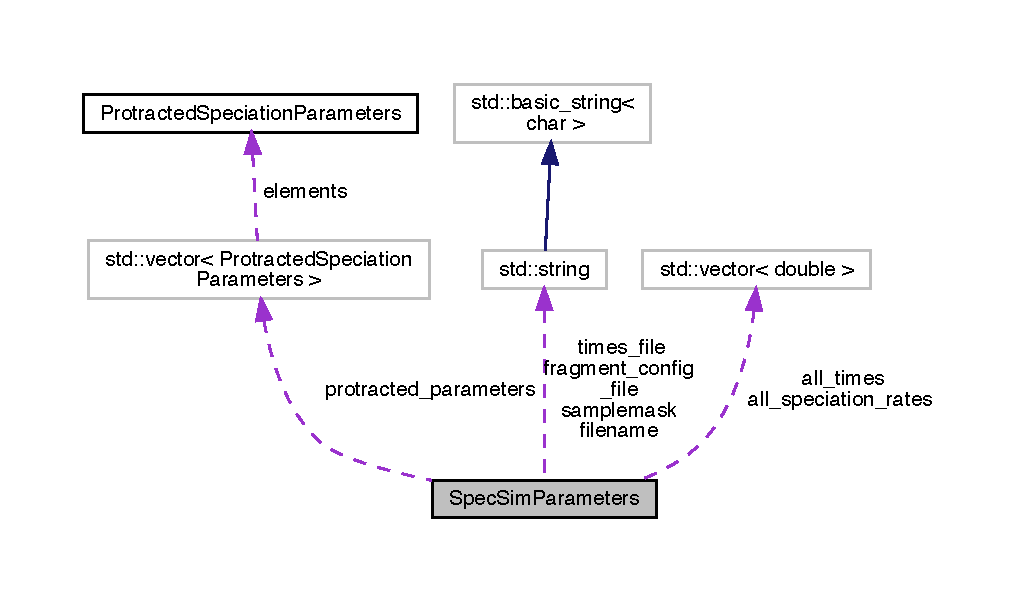
\includegraphics[width=350pt]{struct_spec_sim_parameters__coll__graph}
\end{center}
\end{figure}
\subsection*{Public Member Functions}
\begin{DoxyCompactItemize}
\item 
void \hyperlink{struct_spec_sim_parameters_acbd3e700200cf2bb07b3e58f1dc95ec6}{setup} (string file\+\_\+in, bool use\+\_\+spatial\+\_\+in, string sample\+\_\+file, vector$<$ double $>$ times, string use\+\_\+fragments\+\_\+in, vector$<$ double $>$ speciation\+\_\+rates, vector$<$ double $>$ min\+\_\+speciation\+\_\+gen\+\_\+in, vector$<$ double $>$ max\+\_\+speciation\+\_\+gen\+\_\+in)
\begin{DoxyCompactList}\small\item\em Sets the application arguments for the inputs. Intended for use with the applyspecmodule for integration with python. \end{DoxyCompactList}\item 
void \hyperlink{struct_spec_sim_parameters_acabbdf627ecb8bec48314f7990b9b575}{setup} (string file\+\_\+in, bool use\+\_\+spatial\+\_\+in, string sample\+\_\+file, const vector$<$ double $>$ \&times, string use\+\_\+fragments\+\_\+in, vector$<$ double $>$ speciation\+\_\+rates, vector$<$ double $>$ min\+\_\+speciation\+\_\+gen\+\_\+in, vector$<$ double $>$ max\+\_\+speciation\+\_\+gen\+\_\+in, unsigned long metacommunity\+\_\+size\+\_\+in, double metacommunity\+\_\+speciation\+\_\+rate\+\_\+in)
\begin{DoxyCompactList}\small\item\em Sets the application arguments for the inputs. Intended for use with the applyspecmodule for integration with python. \end{DoxyCompactList}\item 
void \hyperlink{struct_spec_sim_parameters_ae0196a50a551a821b75b6e92a35534a7}{import\+Time\+Config} ()\hypertarget{struct_spec_sim_parameters_ae0196a50a551a821b75b6e92a35534a7}{}\label{struct_spec_sim_parameters_ae0196a50a551a821b75b6e92a35534a7}

\begin{DoxyCompactList}\small\item\em Import the time config file, if there is one. \end{DoxyCompactList}\item 
void \hyperlink{struct_spec_sim_parameters_a10aac8e7ab592f53b071287e60483b88}{wipe} ()\hypertarget{struct_spec_sim_parameters_a10aac8e7ab592f53b071287e60483b88}{}\label{struct_spec_sim_parameters_a10aac8e7ab592f53b071287e60483b88}

\begin{DoxyCompactList}\small\item\em Deletes all the parameters. \end{DoxyCompactList}\item 
void \hyperlink{struct_spec_sim_parameters_a78e27888e92d1b1ddfd9d9a8e129b618}{add\+Time} (double time)
\begin{DoxyCompactList}\small\item\em Adds an additional time to the times vector. \end{DoxyCompactList}\item 
void \hyperlink{struct_spec_sim_parameters_af88d55fcc175d52519a6c2a0843173eb}{add\+Protracted\+Parameters} (double proc\+\_\+spec\+\_\+min, double proc\+\_\+spec\+\_\+max)
\begin{DoxyCompactList}\small\item\em Adds a set of protracted speciation parameters to the protracted parameters vector. \end{DoxyCompactList}\end{DoxyCompactItemize}
\subsection*{Public Attributes}
\begin{DoxyCompactItemize}
\item 
bool {\bfseries use\+\_\+spatial}\hypertarget{struct_spec_sim_parameters_a7baa6db5f411b4fdb9dd5fae0fd25a26}{}\label{struct_spec_sim_parameters_a7baa6db5f411b4fdb9dd5fae0fd25a26}

\item 
bool {\bfseries b\+Multi\+Run}\hypertarget{struct_spec_sim_parameters_a7ca69d2db2aaf8cdcc62b1ec854f72bf}{}\label{struct_spec_sim_parameters_a7ca69d2db2aaf8cdcc62b1ec854f72bf}

\item 
bool {\bfseries use\+\_\+fragments}\hypertarget{struct_spec_sim_parameters_ae2a8648d57c4b7df097bd450ab868e64}{}\label{struct_spec_sim_parameters_ae2a8648d57c4b7df097bd450ab868e64}

\item 
string {\bfseries filename}\hypertarget{struct_spec_sim_parameters_a39beb88bb0ce36265bb0b8c8468cbe48}{}\label{struct_spec_sim_parameters_a39beb88bb0ce36265bb0b8c8468cbe48}

\item 
vector$<$ double $>$ {\bfseries all\+\_\+speciation\+\_\+rates}\hypertarget{struct_spec_sim_parameters_af70bb0689f934fd5ec5ea1878a3e4011}{}\label{struct_spec_sim_parameters_af70bb0689f934fd5ec5ea1878a3e4011}

\item 
string {\bfseries samplemask}\hypertarget{struct_spec_sim_parameters_add68fe2a48b1d80173c5066bf9cd0f6c}{}\label{struct_spec_sim_parameters_add68fe2a48b1d80173c5066bf9cd0f6c}

\item 
string {\bfseries times\+\_\+file}\hypertarget{struct_spec_sim_parameters_a83a3ce34449db0152e0012838c0ac3a6}{}\label{struct_spec_sim_parameters_a83a3ce34449db0152e0012838c0ac3a6}

\item 
vector$<$ double $>$ {\bfseries all\+\_\+times}\hypertarget{struct_spec_sim_parameters_a2a61028935128b94785b6faca0a5788f}{}\label{struct_spec_sim_parameters_a2a61028935128b94785b6faca0a5788f}

\item 
string {\bfseries fragment\+\_\+config\+\_\+file}\hypertarget{struct_spec_sim_parameters_adef81f827b1402d19f318c66f295c62a}{}\label{struct_spec_sim_parameters_adef81f827b1402d19f318c66f295c62a}

\item 
vector$<$ \hyperlink{struct_protracted_speciation_parameters}{Protracted\+Speciation\+Parameters} $>$ {\bfseries protracted\+\_\+parameters}\hypertarget{struct_spec_sim_parameters_a4eba5de74f81f0a81097b4159f6ae797}{}\label{struct_spec_sim_parameters_a4eba5de74f81f0a81097b4159f6ae797}

\item 
unsigned long {\bfseries metacommunity\+\_\+size}\hypertarget{struct_spec_sim_parameters_a5afee22112d2be5b0dc730553e01d2cd}{}\label{struct_spec_sim_parameters_a5afee22112d2be5b0dc730553e01d2cd}

\item 
double {\bfseries metacommunity\+\_\+speciation\+\_\+rate}\hypertarget{struct_spec_sim_parameters_a4aa21c1b3e61729fb6f25d1b5cf38bd2}{}\label{struct_spec_sim_parameters_a4aa21c1b3e61729fb6f25d1b5cf38bd2}

\end{DoxyCompactItemize}


\subsection{Detailed Description}
Contains the simulation parameters that are read from the command line. 

\subsection{Member Function Documentation}
\index{Spec\+Sim\+Parameters@{Spec\+Sim\+Parameters}!add\+Protracted\+Parameters@{add\+Protracted\+Parameters}}
\index{add\+Protracted\+Parameters@{add\+Protracted\+Parameters}!Spec\+Sim\+Parameters@{Spec\+Sim\+Parameters}}
\subsubsection[{\texorpdfstring{add\+Protracted\+Parameters(double proc\+\_\+spec\+\_\+min, double proc\+\_\+spec\+\_\+max)}{addProtractedParameters(double proc_spec_min, double proc_spec_max)}}]{\setlength{\rightskip}{0pt plus 5cm}void Spec\+Sim\+Parameters\+::add\+Protracted\+Parameters (
\begin{DoxyParamCaption}
\item[{double}]{proc\+\_\+spec\+\_\+min, }
\item[{double}]{proc\+\_\+spec\+\_\+max}
\end{DoxyParamCaption}
)\hspace{0.3cm}{\ttfamily [inline]}}\hypertarget{struct_spec_sim_parameters_af88d55fcc175d52519a6c2a0843173eb}{}\label{struct_spec_sim_parameters_af88d55fcc175d52519a6c2a0843173eb}


Adds a set of protracted speciation parameters to the protracted parameters vector. 


\begin{DoxyParams}{Parameters}
{\em proc\+\_\+spec\+\_\+min} & the minimum protracted speciation generation \\
\hline
{\em proc\+\_\+spec\+\_\+max} & the maximum protracted speciation generation \\
\hline
\end{DoxyParams}
\index{Spec\+Sim\+Parameters@{Spec\+Sim\+Parameters}!add\+Time@{add\+Time}}
\index{add\+Time@{add\+Time}!Spec\+Sim\+Parameters@{Spec\+Sim\+Parameters}}
\subsubsection[{\texorpdfstring{add\+Time(double time)}{addTime(double time)}}]{\setlength{\rightskip}{0pt plus 5cm}void Spec\+Sim\+Parameters\+::add\+Time (
\begin{DoxyParamCaption}
\item[{double}]{time}
\end{DoxyParamCaption}
)\hspace{0.3cm}{\ttfamily [inline]}}\hypertarget{struct_spec_sim_parameters_a78e27888e92d1b1ddfd9d9a8e129b618}{}\label{struct_spec_sim_parameters_a78e27888e92d1b1ddfd9d9a8e129b618}


Adds an additional time to the times vector. 


\begin{DoxyParams}{Parameters}
{\em time} & a time to calculate speciation rates at \\
\hline
\end{DoxyParams}
\index{Spec\+Sim\+Parameters@{Spec\+Sim\+Parameters}!setup@{setup}}
\index{setup@{setup}!Spec\+Sim\+Parameters@{Spec\+Sim\+Parameters}}
\subsubsection[{\texorpdfstring{setup(string file\+\_\+in, bool use\+\_\+spatial\+\_\+in, string sample\+\_\+file, vector$<$ double $>$ times, string use\+\_\+fragments\+\_\+in, vector$<$ double $>$ speciation\+\_\+rates, vector$<$ double $>$ min\+\_\+speciation\+\_\+gen\+\_\+in, vector$<$ double $>$ max\+\_\+speciation\+\_\+gen\+\_\+in)}{setup(string file_in, bool use_spatial_in, string sample_file, vector< double > times, string use_fragments_in, vector< double > speciation_rates, vector< double > min_speciation_gen_in, vector< double > max_speciation_gen_in)}}]{\setlength{\rightskip}{0pt plus 5cm}void Spec\+Sim\+Parameters\+::setup (
\begin{DoxyParamCaption}
\item[{string}]{file\+\_\+in, }
\item[{bool}]{use\+\_\+spatial\+\_\+in, }
\item[{string}]{sample\+\_\+file, }
\item[{vector$<$ double $>$}]{times, }
\item[{string}]{use\+\_\+fragments\+\_\+in, }
\item[{vector$<$ double $>$}]{speciation\+\_\+rates, }
\item[{vector$<$ double $>$}]{min\+\_\+speciation\+\_\+gen\+\_\+in, }
\item[{vector$<$ double $>$}]{max\+\_\+speciation\+\_\+gen\+\_\+in}
\end{DoxyParamCaption}
)\hspace{0.3cm}{\ttfamily [inline]}}\hypertarget{struct_spec_sim_parameters_acbd3e700200cf2bb07b3e58f1dc95ec6}{}\label{struct_spec_sim_parameters_acbd3e700200cf2bb07b3e58f1dc95ec6}


Sets the application arguments for the inputs. Intended for use with the applyspecmodule for integration with python. 


\begin{DoxyParams}{Parameters}
{\em file\+\_\+in} & the database to apply speciation rates to \\
\hline
{\em use\+\_\+spatial\+\_\+in} & if true, record full spatial data \\
\hline
{\em sample\+\_\+file} & the sample file to select lineages from the map \\
\hline
{\em times} & vector of times to apply \\
\hline
{\em use\+\_\+fragments\+\_\+in} & fragment file, or \char`\"{}\+T\char`\"{}/\char`\"{}\+F\char`\"{} for automatic detection/no detection \\
\hline
{\em speciation\+\_\+rates} & the speciation rates to apply \\
\hline
{\em min\+\_\+speciation\+\_\+gen\+\_\+in} & the minimum generation rate for speciation in protracted simulations \\
\hline
{\em max\+\_\+speciation\+\_\+gen\+\_\+in} & the maximum generation rate for speciation in protracted simulations \\
\hline
\end{DoxyParams}
\index{Spec\+Sim\+Parameters@{Spec\+Sim\+Parameters}!setup@{setup}}
\index{setup@{setup}!Spec\+Sim\+Parameters@{Spec\+Sim\+Parameters}}
\subsubsection[{\texorpdfstring{setup(string file\+\_\+in, bool use\+\_\+spatial\+\_\+in, string sample\+\_\+file, const vector$<$ double $>$ \&times, string use\+\_\+fragments\+\_\+in, vector$<$ double $>$ speciation\+\_\+rates, vector$<$ double $>$ min\+\_\+speciation\+\_\+gen\+\_\+in, vector$<$ double $>$ max\+\_\+speciation\+\_\+gen\+\_\+in, unsigned long metacommunity\+\_\+size\+\_\+in, double metacommunity\+\_\+speciation\+\_\+rate\+\_\+in)}{setup(string file_in, bool use_spatial_in, string sample_file, const vector< double > &times, string use_fragments_in, vector< double > speciation_rates, vector< double > min_speciation_gen_in, vector< double > max_speciation_gen_in, unsigned long metacommunity_size_in, double metacommunity_speciation_rate_in)}}]{\setlength{\rightskip}{0pt plus 5cm}void Spec\+Sim\+Parameters\+::setup (
\begin{DoxyParamCaption}
\item[{string}]{file\+\_\+in, }
\item[{bool}]{use\+\_\+spatial\+\_\+in, }
\item[{string}]{sample\+\_\+file, }
\item[{const vector$<$ double $>$ \&}]{times, }
\item[{string}]{use\+\_\+fragments\+\_\+in, }
\item[{vector$<$ double $>$}]{speciation\+\_\+rates, }
\item[{vector$<$ double $>$}]{min\+\_\+speciation\+\_\+gen\+\_\+in, }
\item[{vector$<$ double $>$}]{max\+\_\+speciation\+\_\+gen\+\_\+in, }
\item[{unsigned long}]{metacommunity\+\_\+size\+\_\+in, }
\item[{double}]{metacommunity\+\_\+speciation\+\_\+rate\+\_\+in}
\end{DoxyParamCaption}
)\hspace{0.3cm}{\ttfamily [inline]}}\hypertarget{struct_spec_sim_parameters_acabbdf627ecb8bec48314f7990b9b575}{}\label{struct_spec_sim_parameters_acabbdf627ecb8bec48314f7990b9b575}


Sets the application arguments for the inputs. Intended for use with the applyspecmodule for integration with python. 


\begin{DoxyParams}{Parameters}
{\em file\+\_\+in} & the database to apply speciation rates to \\
\hline
{\em use\+\_\+spatial\+\_\+in} & if true, record full spatial data \\
\hline
{\em sample\+\_\+file} & the sample file to select lineages from the map \\
\hline
{\em times} & vector of times to apply \\
\hline
{\em use\+\_\+fragments\+\_\+in} & fragment file, or \char`\"{}\+T\char`\"{}/\char`\"{}\+F\char`\"{} for automatic detection/no detection \\
\hline
{\em speciation\+\_\+rates} & the speciation rates to apply \\
\hline
{\em min\+\_\+speciation\+\_\+gen\+\_\+in} & the minimum generation rate for speciation in protracted simulations \\
\hline
{\em max\+\_\+speciation\+\_\+gen\+\_\+in} & the maximum generation rate for speciation in protracted simulations \\
\hline
{\em metacommunity\+\_\+size\+\_\+in} & \\
\hline
{\em metacommunity\+\_\+speciation\+\_\+rate\+\_\+in} & \\
\hline
\end{DoxyParams}


The documentation for this class was generated from the following file\+:\begin{DoxyCompactItemize}
\item 
necsim/Spec\+Sim\+Parameters.\+h\end{DoxyCompactItemize}

\hypertarget{struct_step}{}\section{Step Class Reference}
\label{struct_step}\index{Step@{Step}}


Stores the elements associated with a single step in a coalescence simulation.  




{\ttfamily \#include $<$Step.\+h$>$}

\subsection*{Public Member Functions}
\begin{DoxyCompactItemize}
\item 
\hyperlink{struct_step_a3f66a321aa9c417352a75c85cff5aca5}{Step} ()
\begin{DoxyCompactList}\small\item\em \hyperlink{struct_step}{Step} constructor. \end{DoxyCompactList}\item 
void \hyperlink{struct_step_ac70e891f944dbeba29bfd1d168b9593c}{wipe\+Data} ()\hypertarget{struct_step_ac70e891f944dbeba29bfd1d168b9593c}{}\label{struct_step_ac70e891f944dbeba29bfd1d168b9593c}

\begin{DoxyCompactList}\small\item\em Removes all stored data from the step. This should be run at the start of a single coalescence step. \end{DoxyCompactList}\end{DoxyCompactItemize}
\subsection*{Public Attributes}
\begin{DoxyCompactItemize}
\item 
unsigned long {\bfseries chosen}\hypertarget{struct_step_a03a0984250a050752ff20129ff457510}{}\label{struct_step_a03a0984250a050752ff20129ff457510}

\item 
unsigned long {\bfseries coalchosen}\hypertarget{struct_step_a5824c6f227fbe3aa249f6067bae0aab2}{}\label{struct_step_a5824c6f227fbe3aa249f6067bae0aab2}

\item 
long {\bfseries oldx}\hypertarget{struct_step_a79f782f87fe4df1f7df10bc6b102530a}{}\label{struct_step_a79f782f87fe4df1f7df10bc6b102530a}

\item 
long {\bfseries oldy}\hypertarget{struct_step_afde730c847c774e13f96c36a2a87a818}{}\label{struct_step_afde730c847c774e13f96c36a2a87a818}

\item 
long {\bfseries oldxwrap}\hypertarget{struct_step_ad627fdb344ea1b6e143bf81794955f9a}{}\label{struct_step_ad627fdb344ea1b6e143bf81794955f9a}

\item 
long {\bfseries oldywrap}\hypertarget{struct_step_ae18da2822c5603f935b02454c1c8f9f3}{}\label{struct_step_ae18da2822c5603f935b02454c1c8f9f3}

\item 
bool {\bfseries coal}\hypertarget{struct_step_a20362fa305c240b197cab6934b4b5087}{}\label{struct_step_a20362fa305c240b197cab6934b4b5087}

\item 
bool {\bfseries b\+Continue\+Sim}\hypertarget{struct_step_a38035eb27c4eb998e5303905356a2cab}{}\label{struct_step_a38035eb27c4eb998e5303905356a2cab}

\item 
unsigned int {\bfseries i\+Auto\+Complete}\hypertarget{struct_step_ad717fe7188f60b50db9675d3cd5ad9d8}{}\label{struct_step_ad717fe7188f60b50db9675d3cd5ad9d8}

\item 
double {\bfseries distance}\hypertarget{struct_step_adcded9ae31a77edc5b91457e38008a7a}{}\label{struct_step_adcded9ae31a77edc5b91457e38008a7a}

\item 
double {\bfseries angle}\hypertarget{struct_step_a92772e673d8c49b468df8710e49cffcb}{}\label{struct_step_a92772e673d8c49b468df8710e49cffcb}

\end{DoxyCompactItemize}


\subsection{Detailed Description}
Stores the elements associated with a single step in a coalescence simulation. 

\begin{DoxyAuthor}{Author}
Sam Thompson 
\end{DoxyAuthor}
\begin{DoxyDate}{Date}
09/08/2017
\end{DoxyDate}
This object should only contain transient variables that are used within a single simulation step and therefore should not be important for pausing/resuming simulations. 

\subsection{Constructor \& Destructor Documentation}
\index{Step@{Step}!Step@{Step}}
\index{Step@{Step}!Step@{Step}}
\subsubsection[{\texorpdfstring{Step()}{Step()}}]{\setlength{\rightskip}{0pt plus 5cm}Step\+::\+Step (
\begin{DoxyParamCaption}
{}
\end{DoxyParamCaption}
)\hspace{0.3cm}{\ttfamily [inline]}}\hypertarget{struct_step_a3f66a321aa9c417352a75c85cff5aca5}{}\label{struct_step_a3f66a321aa9c417352a75c85cff5aca5}


\hyperlink{struct_step}{Step} constructor. 

\begin{DoxyReturn}{Returns}

\end{DoxyReturn}


The documentation for this class was generated from the following file\+:\begin{DoxyCompactItemize}
\item 
\hyperlink{_step_8h}{Step.\+h}\end{DoxyCompactItemize}

\hypertarget{class_tree}{}\section{Tree Class Reference}
\label{class_tree}\index{Tree@{Tree}}


Inheritance diagram for Tree\+:\nopagebreak
\begin{figure}[H]
\begin{center}
\leavevmode
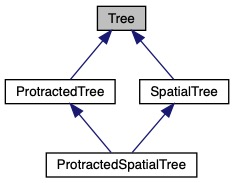
\includegraphics[width=248pt]{class_tree__inherit__graph}
\end{center}
\end{figure}


Collaboration diagram for Tree\+:\nopagebreak
\begin{figure}[H]
\begin{center}
\leavevmode
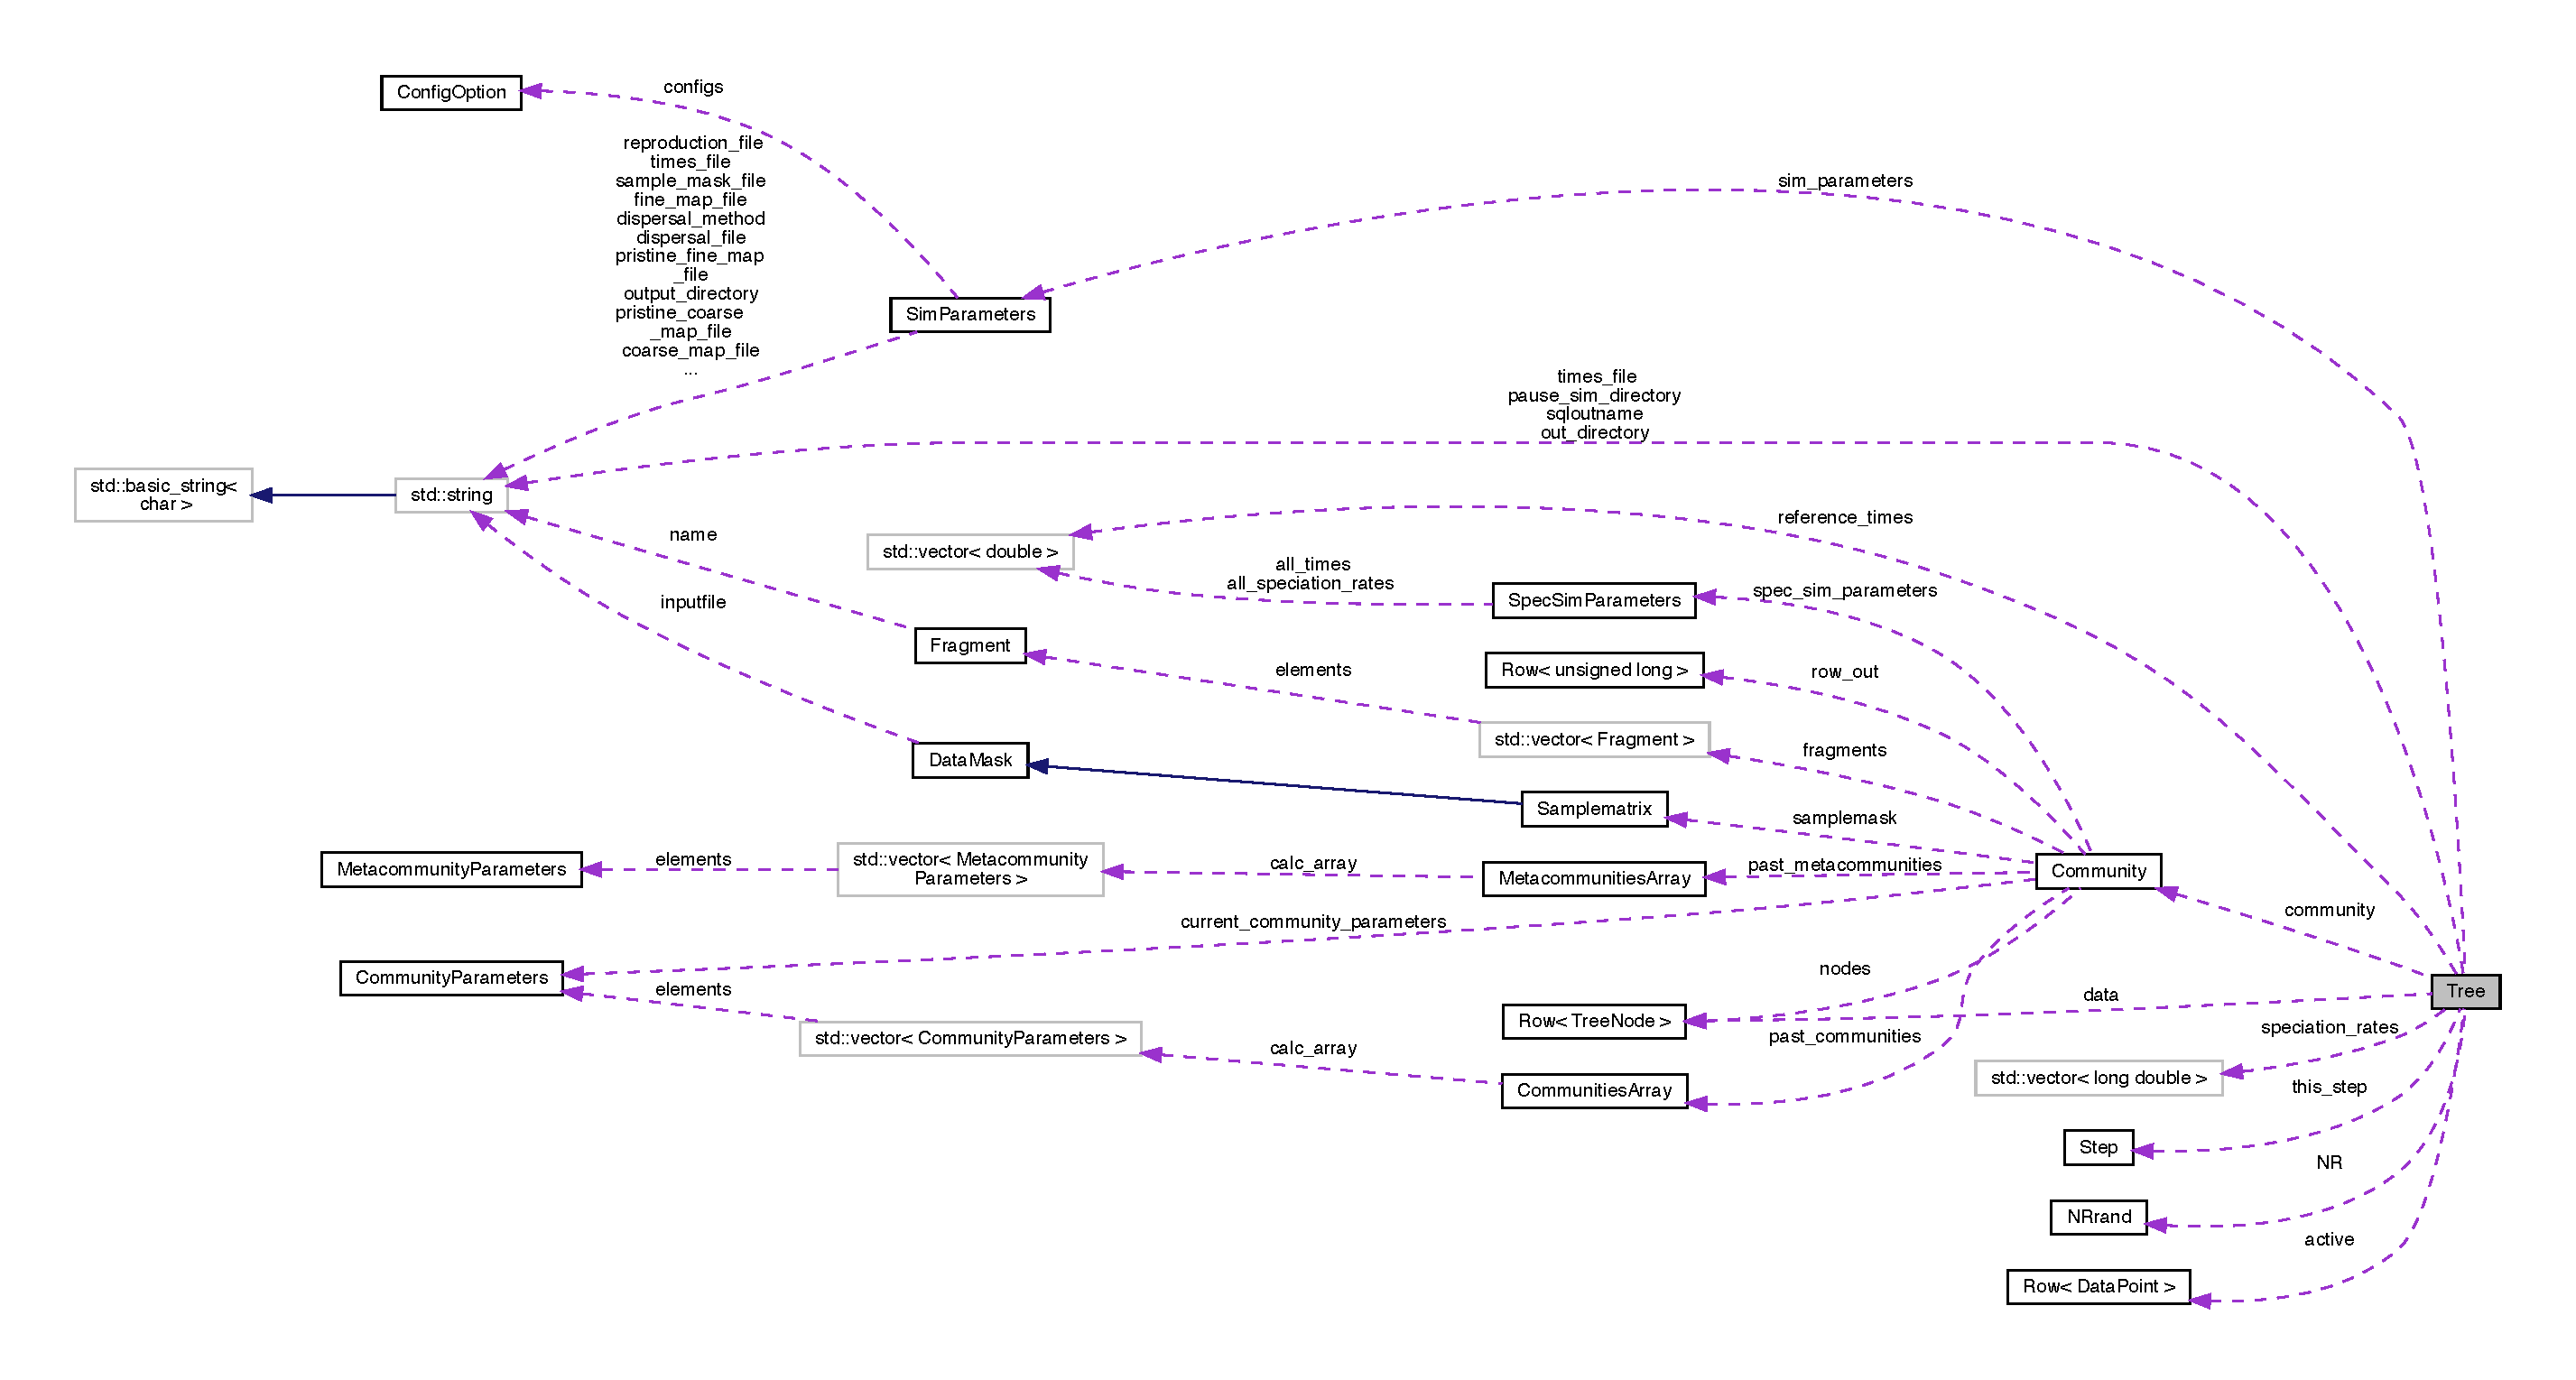
\includegraphics[width=350pt]{class_tree__coll__graph}
\end{center}
\end{figure}
\subsection*{Public Member Functions}
\begin{DoxyCompactItemize}
\item 
void \hyperlink{class_tree_a455d87022772b309a5974ea5f0295139}{import\+Simulation\+Variables} (const string \&configfile)
\begin{DoxyCompactList}\small\item\em Import the simulation variables from the command line structure. \end{DoxyCompactList}\item 
void \hyperlink{class_tree_a029af5f2dc1e33b4eead8110090ac778}{import\+Simulation\+Variables} (\hyperlink{class_config_option}{Config\+Option} config)
\begin{DoxyCompactList}\small\item\em Import the simulation variables from a \hyperlink{class_config_option}{Config\+Option}. \end{DoxyCompactList}\item 
virtual void \hyperlink{class_tree_a0aefbe2466aefd46dec8c4aea4c85c5e}{run\+File\+Checks} ()\hypertarget{class_tree_a0aefbe2466aefd46dec8c4aea4c85c5e}{}\label{class_tree_a0aefbe2466aefd46dec8c4aea4c85c5e}

\begin{DoxyCompactList}\small\item\em Runs the basic file existence checks. Checks for paused simulations and file existence. \end{DoxyCompactList}\item 
void \hyperlink{class_tree_aa31508ea6d5801c6dee17c035f393b60}{wipe\+Simulation\+Variables} ()\hypertarget{class_tree_aa31508ea6d5801c6dee17c035f393b60}{}\label{class_tree_aa31508ea6d5801c6dee17c035f393b60}

\begin{DoxyCompactList}\small\item\em Resets all the simulation variables. \end{DoxyCompactList}\item 
void \hyperlink{class_tree_a62db83e47e5850c6a83793829b22b68b}{internal\+Setup} (const \hyperlink{struct_sim_parameters}{Sim\+Parameters} \&sim\+\_\+parameters\+\_\+in)
\begin{DoxyCompactList}\small\item\em Sets up the simulation parameters from the one provided. \end{DoxyCompactList}\item 
bool \hyperlink{class_tree_a5c6065ede9862e9fb6561eb8beaf5d78}{check\+Output\+Directory} ()
\begin{DoxyCompactList}\small\item\em Asserts that the output directory is not null and exists. If it doesn\textquotesingle{}t exist, it attempts to create it. \end{DoxyCompactList}\item 
void \hyperlink{class_tree_ad0bcc474a9ab1d4e3e2458c4de7304ad}{check\+Sims} ()
\begin{DoxyCompactList}\small\item\em Checks for existing paused simulations to resume from Sets b\+Paused if there are. \end{DoxyCompactList}\item 
void \hyperlink{class_tree_aafaede1da6c79583bf2e28b7a1881a5c}{check\+Sims} (string output\+\_\+dir, long seed, long task)
\begin{DoxyCompactList}\small\item\em Checks for existing paused simulations to resume from. \end{DoxyCompactList}\item 
virtual void \hyperlink{class_tree_ac374d237b7e2e7e11f6a0ff395003635}{set\+Parameters} ()\hypertarget{class_tree_ac374d237b7e2e7e11f6a0ff395003635}{}\label{class_tree_ac374d237b7e2e7e11f6a0ff395003635}

\begin{DoxyCompactList}\small\item\em Move the parameters from the sim\+\_\+parameters object to their relevant parameters. \end{DoxyCompactList}\item 
virtual void \hyperlink{class_tree_a891764ffc1e29d3edbe0fd08e67a184b}{set\+Protracted\+Variables} (double speciation\+\_\+gen\+\_\+min, double speciation\+\_\+gen\+\_\+max)
\begin{DoxyCompactList}\small\item\em Sets the protracted variables. \end{DoxyCompactList}\item 
bool \hyperlink{class_tree_ae07761c0a91a44ebe459904b1b8ffb43}{has\+Paused} ()
\begin{DoxyCompactList}\small\item\em Gets the has\+\_\+paused variable for resuming sims. \end{DoxyCompactList}\item 
vector$<$ double $>$ \hyperlink{class_tree_ac03c034a5730ee4f4d8727aace776412}{get\+Temporal\+Sampling} ()\hypertarget{class_tree_ac03c034a5730ee4f4d8727aace776412}{}\label{class_tree_ac03c034a5730ee4f4d8727aace776412}

\begin{DoxyCompactList}\small\item\em Gets the map autocorrel times. \end{DoxyCompactList}\item 
long long \hyperlink{class_tree_a857521315ca6bd9b3300d099488d74f1}{get\+Seed} ()
\begin{DoxyCompactList}\small\item\em Getter for the simulation seed. \end{DoxyCompactList}\item 
void \hyperlink{class_tree_ab240ab1988cbde281a6811b3fdc1dd5d}{set\+Seed} (long long seed\+\_\+in)
\begin{DoxyCompactList}\small\item\em Sets the simulation seed for the random number generator. \end{DoxyCompactList}\item 
virtual unsigned long \hyperlink{class_tree_a1e0685310a5a9bca4d6069e8d4ce1f1b}{get\+Initial\+Count} ()
\begin{DoxyCompactList}\small\item\em Gets the initial number of individuals. \end{DoxyCompactList}\item 
unsigned long \hyperlink{class_tree_a869ab0aba75336f737cbb137c74b8abc}{set\+Object\+Sizes} ()
\begin{DoxyCompactList}\small\item\em Sets the sizes of grid, active and data, based on the number of individuals counted from the samplemask. \end{DoxyCompactList}\item 
virtual void \hyperlink{class_tree_aec10ea2b720edc13a38310afdfe2b6e4}{setup} ()
\begin{DoxyCompactList}\small\item\em The setup function for generating the simulation objects. \end{DoxyCompactList}\item 
void \hyperlink{class_tree_aec2640897132a1b667e852bbafc14c78}{set\+Initial\+Values} ()\hypertarget{class_tree_aec2640897132a1b667e852bbafc14c78}{}\label{class_tree_aec2640897132a1b667e852bbafc14c78}

\begin{DoxyCompactList}\small\item\em Sets the starting values for required parameters. \end{DoxyCompactList}\item 
void \hyperlink{class_tree_a1ba0f5d27c6ef6e9e17f988aff2dfe65}{set\+Sim\+Start\+Variables} ()
\begin{DoxyCompactList}\small\item\em Sets the variables at the start of a simulation for temporary data. \end{DoxyCompactList}\item 
void \hyperlink{class_tree_ab71da7797a6586ddd948661c34ce4788}{print\+Setup} ()
\begin{DoxyCompactList}\small\item\em Prints the statement for the setup initiation. \end{DoxyCompactList}\item 
void \hyperlink{class_tree_ae3fb33c46cf7e3af44604a9875b375a3}{set\+Times} ()\hypertarget{class_tree_ae3fb33c46cf7e3af44604a9875b375a3}{}\label{class_tree_ae3fb33c46cf7e3af44604a9875b375a3}

\begin{DoxyCompactList}\small\item\em Sets the temporal sampling points from the time config file. \end{DoxyCompactList}\item 
void \hyperlink{class_tree_a25f082da13789dfa3fefcbcfd08b4dfe}{determine\+Speciation\+Rates} ()
\begin{DoxyCompactList}\small\item\em Determines the speciation rates to apply and then applies them to the coalescence tree post-\/simulation. \end{DoxyCompactList}\item 
void \hyperlink{class_tree_a38488499b196d3f5ee40b2a68fe3279e}{add\+Speciation\+Rates} (vector$<$ long double $>$ spec\+\_\+rates\+\_\+in)\hypertarget{class_tree_a38488499b196d3f5ee40b2a68fe3279e}{}\label{class_tree_a38488499b196d3f5ee40b2a68fe3279e}

\begin{DoxyCompactList}\small\item\em Adds the speciation rates to those to be applied. \end{DoxyCompactList}\item 
void \hyperlink{class_tree_a50b3d13d4032e0d7a69890b9bd7f84fa}{generate\+Objects} ()\hypertarget{class_tree_a50b3d13d4032e0d7a69890b9bd7f84fa}{}\label{class_tree_a50b3d13d4032e0d7a69890b9bd7f84fa}

\begin{DoxyCompactList}\small\item\em Assigns the objects sizes in memory and fills with the starting lineages. \end{DoxyCompactList}\item 
virtual unsigned long \hyperlink{class_tree_a4af845777294c9116c60115e651620b4}{fill\+Objects} (const unsigned long \&initial\+\_\+count)
\begin{DoxyCompactList}\small\item\em Fills the active and data objects with the starting lineages. \end{DoxyCompactList}\item 
virtual bool \hyperlink{class_tree_afe75245862a1c40030c1c8607518cf8d}{run\+Simulation} ()
\begin{DoxyCompactList}\small\item\em Run the entire simulation given the start conditions already defined by \hyperlink{class_tree_aec10ea2b720edc13a38310afdfe2b6e4}{setup()} \end{DoxyCompactList}\item 
void \hyperlink{class_tree_a95360a2f62ef0eb436d586552b299e1f}{write\+Sim\+Start\+To\+Console} ()\hypertarget{class_tree_a95360a2f62ef0eb436d586552b299e1f}{}\label{class_tree_a95360a2f62ef0eb436d586552b299e1f}

\begin{DoxyCompactList}\small\item\em Writes to the console that the simulation is beginning. \end{DoxyCompactList}\item 
void \hyperlink{class_tree_a37de93174eece50a2fc082b683d97047}{write\+Step\+To\+Console} ()\hypertarget{class_tree_a37de93174eece50a2fc082b683d97047}{}\label{class_tree_a37de93174eece50a2fc082b683d97047}

\begin{DoxyCompactList}\small\item\em Write the step counter to console. This function should only be called in debugging mode. \end{DoxyCompactList}\item 
virtual void \hyperlink{class_tree_a3f0c8928b4b72fb6f03cabd4d0e04457}{increment\+Generation} ()\hypertarget{class_tree_a3f0c8928b4b72fb6f03cabd4d0e04457}{}\label{class_tree_a3f0c8928b4b72fb6f03cabd4d0e04457}

\begin{DoxyCompactList}\small\item\em Increments the generation counter and step references. \end{DoxyCompactList}\item 
void \hyperlink{class_tree_a23803bddf46ad28a1bdd46bf05693b1f}{choose\+Random\+Lineage} ()
\begin{DoxyCompactList}\small\item\em Chooses a random lineage from active. \end{DoxyCompactList}\item 
virtual void \hyperlink{class_tree_ad65e94936001675b8bc908cf77e0cb53}{update\+Step\+Coalescence\+Variables} ()\hypertarget{class_tree_ad65e94936001675b8bc908cf77e0cb53}{}\label{class_tree_ad65e94936001675b8bc908cf77e0cb53}

\begin{DoxyCompactList}\small\item\em Updates the coalescence variables in the step object. \end{DoxyCompactList}\item 
void \hyperlink{class_tree_a05c9e44f1a4d7af83e65b6c4565b1b28}{speciation} (const unsigned long \&chosen)
\begin{DoxyCompactList}\small\item\em Speciation to supplied lineage. \end{DoxyCompactList}\item 
virtual void \hyperlink{class_tree_a32e12cc62ce2d9ae893214b1f4cfad1f}{speciate\+Lineage} (const unsigned long \&data\+\_\+position)
\begin{DoxyCompactList}\small\item\em Performs the actual speciation. \end{DoxyCompactList}\item 
virtual void \hyperlink{class_tree_ad74c05729c9e5235ab0fa6e34260093a}{remove\+Old\+Position} (const unsigned long \&chosen)
\begin{DoxyCompactList}\small\item\em Removes the old position within active. \end{DoxyCompactList}\item 
virtual void \hyperlink{class_tree_ab1be13d2e99a4445a7cc84f907e0c90e}{switch\+Positions} (const unsigned long \&chosen)
\begin{DoxyCompactList}\small\item\em Switches the chosen position with the endactive position. \end{DoxyCompactList}\item 
virtual void \hyperlink{class_tree_a0dc015aa5a45d2a75d80456d680172ac}{calc\+Next\+Step} ()\hypertarget{class_tree_a0dc015aa5a45d2a75d80456d680172ac}{}\label{class_tree_a0dc015aa5a45d2a75d80456d680172ac}

\begin{DoxyCompactList}\small\item\em Calculates the next step for the simulation. \end{DoxyCompactList}\item 
virtual bool \hyperlink{class_tree_abc9389511e1aecf5e573315fc8f4d77c}{calc\+Speciation} (const long double \&random\+\_\+number, const long double \&speciation\+\_\+rate, const unsigned long \&no\+\_\+generations)
\begin{DoxyCompactList}\small\item\em Calculates the speciation probability from the random number, speciation rate and number of generations a lineage has existed for. \end{DoxyCompactList}\item 
void \hyperlink{class_tree_a16eedb70009e7570d933f88e8ce44117}{coalescence\+Event} (const unsigned long \&chosen, unsigned long \&coalchosen)
\begin{DoxyCompactList}\small\item\em Perform the coalescence between lineages. Once coalesced, lineages are removed from the active scope. \end{DoxyCompactList}\item 
void \hyperlink{class_tree_afcbe72c55b38c94ae17de9c2e1dd3a7f}{check\+Time\+Update} ()\hypertarget{class_tree_afcbe72c55b38c94ae17de9c2e1dd3a7f}{}\label{class_tree_afcbe72c55b38c94ae17de9c2e1dd3a7f}

\begin{DoxyCompactList}\small\item\em Checks if the number of lineages should be expanded at another sample point. \end{DoxyCompactList}\item 
virtual void \hyperlink{class_tree_a8bfa9a86f122b21900ec33ab4b1e323f}{add\+Lineages} (double generation\+\_\+in)
\begin{DoxyCompactList}\small\item\em Adds the required lineages at the generation time. \end{DoxyCompactList}\item 
void \hyperlink{class_tree_ab8a62d0ca2b1746676073e3f33e2a949}{check\+Sim\+Size} (unsigned long req\+\_\+data, unsigned long req\+\_\+active)
\begin{DoxyCompactList}\small\item\em Checks the size of the main active and data objects is large enough. \end{DoxyCompactList}\item 
void \hyperlink{class_tree_a0973cc37d9b95144db76d36cb363caca}{make\+Tip} (const unsigned long \&tmp\+\_\+active, const double \&generation\+\_\+in)
\begin{DoxyCompactList}\small\item\em Sets the active reference to a tip, if it isn\textquotesingle{}t one already. Otherwise, creates a new tip for the new generation time. \end{DoxyCompactList}\item 
void \hyperlink{class_tree_a6af2aaa691ffbb9899e3f070a715e371}{convert\+Tip} (unsigned long i, double generationin)
\begin{DoxyCompactList}\small\item\em Creates a new reference in data containing the tip with a new generation counter. \end{DoxyCompactList}\item 
bool \hyperlink{class_tree_afd6bd75c301d2f57c4997fcfc92f192e}{stop\+Simulation} ()
\begin{DoxyCompactList}\small\item\em Finalises the simulation, and performs the correct tasks depending if the sim has been paused or finished. \end{DoxyCompactList}\item 
void \hyperlink{class_tree_aa6349a32b3fcfb82a5f8311b11db3982}{apply\+Spec\+Rate} (long double sr, double t)
\begin{DoxyCompactList}\small\item\em Applies the given speciation rate to the tree. \end{DoxyCompactList}\item 
void \hyperlink{class_tree_ac89abe0404d05d0363258b72cb80700b}{apply\+Spec\+Rate\+Internal} (long double sr, double t)
\begin{DoxyCompactList}\small\item\em Applies the given speciation rate to the tree, but does not output to a file. Instead returns a pointer to the nodes object. \end{DoxyCompactList}\item 
\hyperlink{class_row}{Row}$<$ unsigned long $>$ $\ast$ \hyperlink{class_tree_a49a94b2218f7ae127a53af4a58d02b06}{get\+Cumulative\+Abundances} ()
\begin{DoxyCompactList}\small\item\em Gets the sorted cumulative species abundances from the contained Tree\+List. \end{DoxyCompactList}\item 
void \hyperlink{class_tree_a9997b98824a786d9843a3df40de1226a}{setup\+Tree\+Generation} (long double sr, double t)
\begin{DoxyCompactList}\small\item\em Sets up the generation of the tree object. \end{DoxyCompactList}\item 
void \hyperlink{class_tree_ab699328f13b22f48faa63a5638e907db}{apply\+Spec\+Rate} (long double sr)
\begin{DoxyCompactList}\small\item\em Overloaded version of apply\+Spec\+Rates for the default generation (0.\+0). \end{DoxyCompactList}\item 
void \hyperlink{class_tree_acfc7efdec999f6dbf2ac089514d22091}{apply\+Multiple\+Rates} ()
\begin{DoxyCompactList}\small\item\em Applies multiple speciation rates to the coalescence tree, ignoring repeated speciation rates. \end{DoxyCompactList}\item 
virtual bool \hyperlink{class_tree_aa23a57f7863d58384f61d464d998ab3c}{get\+Protracted} ()
\begin{DoxyCompactList}\small\item\em Gets the protractedness of the simulation. Overridden by protracted child classes. \end{DoxyCompactList}\item 
virtual string \hyperlink{class_tree_a34c0808026bf00546c8f9786376be730}{get\+Protracted\+Variables} ()
\begin{DoxyCompactList}\small\item\em Gets the protracted variables and returns them as a single, newline separated string. This method is intended to be overridden in derived classes. \end{DoxyCompactList}\item 
virtual double \hyperlink{class_tree_a6ffc42e941f352cd74f01f6f7011f00b}{get\+Protracted\+Generation\+Min} ()
\begin{DoxyCompactList}\small\item\em Gets the minimum number of generations a lineage must exist. \end{DoxyCompactList}\item 
virtual double \hyperlink{class_tree_a0c5e746982a87f24c083f4534bf92b45}{get\+Protracted\+Generation\+Max} ()
\begin{DoxyCompactList}\small\item\em Gets the maximum number of generations a lineage can exist. \end{DoxyCompactList}\item 
void \hyperlink{class_tree_a8cd3db7add1884ea53b0d98002d39cd3}{sql\+Output} ()
\begin{DoxyCompactList}\small\item\em Copy the in-\/memory database to file. \end{DoxyCompactList}\item 
void \hyperlink{class_tree_afdf680e187c25ed39d1e66542ce44cc3}{output\+Data} ()\hypertarget{class_tree_afdf680e187c25ed39d1e66542ce44cc3}{}\label{class_tree_afdf680e187c25ed39d1e66542ce44cc3}

\begin{DoxyCompactList}\small\item\em Outputs important simulation data to a csv file. Overloaded version which automatically calls \hyperlink{class_tree_a2d2065bbebee8b55270d2691d40cd974}{sort\+Data()} if no species richness is provided. \end{DoxyCompactList}\item 
void \hyperlink{class_tree_a5acf7d0eea9ea2ef4928bb6691b87724}{output\+Data} (unsigned long species\+\_\+richness)
\begin{DoxyCompactList}\small\item\em Outputs important simulation data to a csv file. This function will likely be remove in future versions as all simulation output is now contained in an S\+Q\+Lite database. \end{DoxyCompactList}\item 
unsigned long \hyperlink{class_tree_a2d2065bbebee8b55270d2691d40cd974}{sort\+Data} ()\hypertarget{class_tree_a2d2065bbebee8b55270d2691d40cd974}{}\label{class_tree_a2d2065bbebee8b55270d2691d40cd974}

\begin{DoxyCompactList}\small\item\em Sort and process the species list so that the useful information can be extracted from it. \end{DoxyCompactList}\item 
void \hyperlink{class_tree_ab8785fc9e27868a56335048321c13290}{write\+Times} ()\hypertarget{class_tree_ab8785fc9e27868a56335048321c13290}{}\label{class_tree_ab8785fc9e27868a56335048321c13290}

\begin{DoxyCompactList}\small\item\em Writes the times to the terminal for simulation information. \end{DoxyCompactList}\item 
void \hyperlink{class_tree_a9e240bbfc3139b290a0dead741f560bf}{open\+S\+Q\+L\+Database} ()\hypertarget{class_tree_a9e240bbfc3139b290a0dead741f560bf}{}\label{class_tree_a9e240bbfc3139b290a0dead741f560bf}

\begin{DoxyCompactList}\small\item\em Opens a connection to the in-\/memory database, or the on-\/disk database, depending on the compilation options. \end{DoxyCompactList}\item 
void \hyperlink{class_tree_ae784a6ed362f6c5263ee797759f715b6}{sql\+Create} ()\hypertarget{class_tree_ae784a6ed362f6c5263ee797759f715b6}{}\label{class_tree_ae784a6ed362f6c5263ee797759f715b6}

\begin{DoxyCompactList}\small\item\em Generates the S\+QL database file from the full simulation data. This allows for greater analysis of the data after completion of the simulation. \end{DoxyCompactList}\item 
void \hyperlink{class_tree_a199f47b62b9b10917ff8b89d20c543a7}{sql\+Create\+Simulation\+Parameters} ()\hypertarget{class_tree_a199f47b62b9b10917ff8b89d20c543a7}{}\label{class_tree_a199f47b62b9b10917ff8b89d20c543a7}

\begin{DoxyCompactList}\small\item\em Creates the S\+I\+M\+U\+L\+A\+T\+I\+O\+N\+\_\+\+P\+A\+R\+A\+M\+E\+T\+E\+RS table in the S\+QL database. \end{DoxyCompactList}\item 
virtual string \hyperlink{class_tree_aed6504b4f759fb31fdeb61cd03b2b3f9}{simulation\+Parameters\+Sql\+Insertion} ()
\begin{DoxyCompactList}\small\item\em Creates a string containing the S\+QL insertion statement for the simulation parameters. \end{DoxyCompactList}\item 
virtual string \hyperlink{class_tree_aa8bb5d93c7992404ede0a49bb69ccd1f}{protracted\+Vars\+To\+String} ()
\begin{DoxyCompactList}\small\item\em Outputs the protracted variables to a string. \end{DoxyCompactList}\item 
virtual void \hyperlink{class_tree_ae5308f74e982485ac444aa394b952152}{sim\+Pause} ()\hypertarget{class_tree_ae5308f74e982485ac444aa394b952152}{}\label{class_tree_ae5308f74e982485ac444aa394b952152}

\begin{DoxyCompactList}\small\item\em Pause the simulation and dump data from memory. \end{DoxyCompactList}\item 
string \hyperlink{class_tree_a9b2df7fd1b61d3d70ac630f7fbfd683d}{initiate\+Pause} ()\hypertarget{class_tree_a9b2df7fd1b61d3d70ac630f7fbfd683d}{}\label{class_tree_a9b2df7fd1b61d3d70ac630f7fbfd683d}

\begin{DoxyCompactList}\small\item\em Checks the output folder exists and initiates the pause. \end{DoxyCompactList}\item 
void \hyperlink{class_tree_a4c2988184328a5236ca61f16744cfac2}{dump\+Main} (string pause\+\_\+folder)
\begin{DoxyCompactList}\small\item\em Saves the main simulation variables to file. \end{DoxyCompactList}\item 
void \hyperlink{class_tree_aca99503f49b91baae7401423fe547daf}{dump\+Active} (string pause\+\_\+folder)
\begin{DoxyCompactList}\small\item\em Saves the active object to file. \end{DoxyCompactList}\item 
void \hyperlink{class_tree_acd23fa139c7d097315c9479187b1a674}{dump\+Data} (string pause\+\_\+folder)
\begin{DoxyCompactList}\small\item\em Saves the data object to file. \end{DoxyCompactList}\item 
void \hyperlink{class_tree_a3fddb18a5d19b64dec378dca3d3fea31}{complete\+Pause} ()\hypertarget{class_tree_a3fddb18a5d19b64dec378dca3d3fea31}{}\label{class_tree_a3fddb18a5d19b64dec378dca3d3fea31}

\begin{DoxyCompactList}\small\item\em Completes the pause routine and outputs the sql dump. \end{DoxyCompactList}\item 
void \hyperlink{class_tree_ac545d844141db977920fc9fd76ce9dbb}{set\+Resume\+Parameters} (string pausedir, string outdir, unsigned long seed, unsigned long task, unsigned long new\+\_\+max\+\_\+time)
\begin{DoxyCompactList}\small\item\em Sets the resume variables so that the simulation can be resumed. \end{DoxyCompactList}\item 
void \hyperlink{class_tree_aeade4bccb8394937a53bc4fbcf2b4300}{set\+Resume\+Parameters} ()\hypertarget{class_tree_aeade4bccb8394937a53bc4fbcf2b4300}{}\label{class_tree_aeade4bccb8394937a53bc4fbcf2b4300}

\begin{DoxyCompactList}\small\item\em Sets the resume variables to the defaults. \end{DoxyCompactList}\item 
virtual void \hyperlink{class_tree_af57075728924141c7b6d311822a22dc0}{load\+Main\+Save} ()\hypertarget{class_tree_af57075728924141c7b6d311822a22dc0}{}\label{class_tree_af57075728924141c7b6d311822a22dc0}

\begin{DoxyCompactList}\small\item\em Loads the main simulation parameters from the save file into memory. \end{DoxyCompactList}\item 
void \hyperlink{class_tree_af7db53d4870d845741d3159f57b73b30}{load\+Data\+Save} ()\hypertarget{class_tree_af7db53d4870d845741d3159f57b73b30}{}\label{class_tree_af7db53d4870d845741d3159f57b73b30}

\begin{DoxyCompactList}\small\item\em Loads the data object from the save file into memory. \end{DoxyCompactList}\item 
void \hyperlink{class_tree_af145148202f11654d6d6a15a6c021924}{load\+Active\+Save} ()\hypertarget{class_tree_af145148202f11654d6d6a15a6c021924}{}\label{class_tree_af145148202f11654d6d6a15a6c021924}

\begin{DoxyCompactList}\small\item\em Loads the active object from the save file into memory. \end{DoxyCompactList}\item 
void \hyperlink{class_tree_a8cfe5d30d53d702f18cd67981e2c9acb}{initiate\+Resume} ()\hypertarget{class_tree_a8cfe5d30d53d702f18cd67981e2c9acb}{}\label{class_tree_a8cfe5d30d53d702f18cd67981e2c9acb}

\begin{DoxyCompactList}\small\item\em Checks for resuming and prints to the terminal. \end{DoxyCompactList}\item 
virtual void \hyperlink{class_tree_a3d614f3848dc7acab168642efe345569}{sim\+Resume} ()
\begin{DoxyCompactList}\small\item\em Resumes the simulation from a previous state. \end{DoxyCompactList}\end{DoxyCompactItemize}
\subsection*{Protected Attributes}
\begin{DoxyCompactItemize}
\item 
\hyperlink{class_row}{Row}$<$ \hyperlink{class_tree_node}{Tree\+Node} $>$ {\bfseries data}\hypertarget{class_tree_a5983af6c56e41be51be0766941093b4b}{}\label{class_tree_a5983af6c56e41be51be0766941093b4b}

\item 
unsigned long {\bfseries enddata}\hypertarget{class_tree_a50344999e6b64d15eef935b1f6023471}{}\label{class_tree_a50344999e6b64d15eef935b1f6023471}

\item 
\hyperlink{struct_sim_parameters}{Sim\+Parameters} {\bfseries sim\+\_\+parameters}\hypertarget{class_tree_a63c399793a209332ad0f5da7fc830d56}{}\label{class_tree_a63c399793a209332ad0f5da7fc830d56}

\item 
\hyperlink{class_n_rrand}{N\+Rrand} {\bfseries NR}\hypertarget{class_tree_aa7df162306777b040a9a2aac543e6801}{}\label{class_tree_aa7df162306777b040a9a2aac543e6801}

\item 
vector$<$ long double $>$ {\bfseries speciation\+\_\+rates}\hypertarget{class_tree_a61b4349fe78d09ac06eff4b7d6833105}{}\label{class_tree_a61b4349fe78d09ac06eff4b7d6833105}

\item 
bool {\bfseries seeded}\hypertarget{class_tree_a78935befd45946b8e69023bffca59c1d}{}\label{class_tree_a78935befd45946b8e69023bffca59c1d}

\item 
long long {\bfseries the\+\_\+seed}\hypertarget{class_tree_acf483ed0a44629c9aa4690a08017ee35}{}\label{class_tree_acf483ed0a44629c9aa4690a08017ee35}

\item 
long long {\bfseries the\+\_\+task}\hypertarget{class_tree_a9f74137d5c9c5529ec9a06f88dfa6960}{}\label{class_tree_a9f74137d5c9c5529ec9a06f88dfa6960}

\item 
string {\bfseries times\+\_\+file}\hypertarget{class_tree_a5e031ea8d94f48288547116a9e7d7add}{}\label{class_tree_a5e031ea8d94f48288547116a9e7d7add}

\item 
vector$<$ double $>$ {\bfseries reference\+\_\+times}\hypertarget{class_tree_a56bb1ea64368f5b705360a435350f9d5}{}\label{class_tree_a56bb1ea64368f5b705360a435350f9d5}

\item 
bool {\bfseries uses\+\_\+temporal\+\_\+sampling}\hypertarget{class_tree_abed1688c75153c4af4e8c574a26dd636}{}\label{class_tree_abed1688c75153c4af4e8c574a26dd636}

\item 
time\+\_\+t {\bfseries start}\hypertarget{class_tree_ac077d686ee96b123aa779e8a8a5de3ce}{}\label{class_tree_ac077d686ee96b123aa779e8a8a5de3ce}

\item 
time\+\_\+t {\bfseries sim\+\_\+start}\hypertarget{class_tree_a01cc9b30f2b10b9f51b218df25b13b09}{}\label{class_tree_a01cc9b30f2b10b9f51b218df25b13b09}

\item 
time\+\_\+t {\bfseries sim\+\_\+end}\hypertarget{class_tree_a26100477c7e58a9e0a90cdee1379ed69}{}\label{class_tree_a26100477c7e58a9e0a90cdee1379ed69}

\item 
time\+\_\+t {\bfseries now}\hypertarget{class_tree_a5510d0fb5deb23fd39a2619d104f85fa}{}\label{class_tree_a5510d0fb5deb23fd39a2619d104f85fa}

\item 
time\+\_\+t {\bfseries sim\+\_\+finish}\hypertarget{class_tree_ac399ba59be9dc33a04223d10a82ee5ee}{}\label{class_tree_ac399ba59be9dc33a04223d10a82ee5ee}

\item 
time\+\_\+t {\bfseries out\+\_\+finish}\hypertarget{class_tree_a5ee1fa5adf72bb599badc041fbee7d09}{}\label{class_tree_a5ee1fa5adf72bb599badc041fbee7d09}

\item 
time\+\_\+t {\bfseries time\+\_\+taken}\hypertarget{class_tree_abd18bb487c0192588b6bed6f00bcfd07}{}\label{class_tree_abd18bb487c0192588b6bed6f00bcfd07}

\item 
\hyperlink{class_row}{Row}$<$ \hyperlink{class_data_point}{Data\+Point} $>$ {\bfseries active}\hypertarget{class_tree_a047b331de4979aa4713c69f09237ac35}{}\label{class_tree_a047b331de4979aa4713c69f09237ac35}

\item 
unsigned long {\bfseries endactive}\hypertarget{class_tree_ab478831f09c135bc9a4bc991c9fd5076}{}\label{class_tree_ab478831f09c135bc9a4bc991c9fd5076}

\item 
unsigned long {\bfseries startendactive}\hypertarget{class_tree_a3f1a90ab7ef917a996790e5ddfcebf85}{}\label{class_tree_a3f1a90ab7ef917a996790e5ddfcebf85}

\item 
unsigned long {\bfseries maxsimsize}\hypertarget{class_tree_a0244ee15452c38393246147d93836b4d}{}\label{class_tree_a0244ee15452c38393246147d93836b4d}

\item 
\hyperlink{class_community}{Community} {\bfseries community}\hypertarget{class_tree_adbb8b625d03dbcdca00f3d8d4b4a50df}{}\label{class_tree_adbb8b625d03dbcdca00f3d8d4b4a50df}

\item 
long {\bfseries steps}\hypertarget{class_tree_ae7d33b8c16eeb8cb0c7f96dbfbc61b4e}{}\label{class_tree_ae7d33b8c16eeb8cb0c7f96dbfbc61b4e}

\item 
unsigned long {\bfseries maxtime}\hypertarget{class_tree_a1868cf626a0b12f21a038989d4eca210}{}\label{class_tree_a1868cf626a0b12f21a038989d4eca210}

\item 
double {\bfseries generation}\hypertarget{class_tree_a84cc46d51045ff3b161ee8788950e0c2}{}\label{class_tree_a84cc46d51045ff3b161ee8788950e0c2}

\item 
long {\bfseries deme}\hypertarget{class_tree_a9fe104115b4593c772c03b57b82ff0de}{}\label{class_tree_a9fe104115b4593c772c03b57b82ff0de}

\item 
double {\bfseries deme\+\_\+sample}\hypertarget{class_tree_ac7a1d0583d3dcb55c50fec0e1fd57985}{}\label{class_tree_ac7a1d0583d3dcb55c50fec0e1fd57985}

\item 
long double {\bfseries spec}\hypertarget{class_tree_a586678f7084086add3a4136476abd375}{}\label{class_tree_a586678f7084086add3a4136476abd375}

\item 
string {\bfseries out\+\_\+directory}\hypertarget{class_tree_a85615771af7b568adca1b801995cfdc7}{}\label{class_tree_a85615771af7b568adca1b801995cfdc7}

\item 
sqlite3 $\ast$ {\bfseries database}\hypertarget{class_tree_aae24ce11e30fbd74fe078b23b46c14cd}{}\label{class_tree_aae24ce11e30fbd74fe078b23b46c14cd}

\item 
bool {\bfseries sim\+\_\+complete}\hypertarget{class_tree_a07f9982fd6f6243c78ef42371603bbe4}{}\label{class_tree_a07f9982fd6f6243c78ef42371603bbe4}

\item 
bool {\bfseries has\+\_\+imported\+\_\+vars}\hypertarget{class_tree_a97bde28466a098bb9e58c1bd5610fd68}{}\label{class_tree_a97bde28466a098bb9e58c1bd5610fd68}

\item 
sqlite3 $\ast$ {\bfseries outdatabase}\hypertarget{class_tree_afd585c8a4bdb86461780418f7b886abd}{}\label{class_tree_afd585c8a4bdb86461780418f7b886abd}

\item 
\hyperlink{struct_step}{Step} {\bfseries this\+\_\+step}\hypertarget{class_tree_af7de4d4f04360edcbe2a20db882b1f87}{}\label{class_tree_af7de4d4f04360edcbe2a20db882b1f87}

\item 
string {\bfseries sql\+\_\+output\+\_\+database}\hypertarget{class_tree_a80d3e92108eb472df49640a661ef4f7d}{}\label{class_tree_a80d3e92108eb472df49640a661ef4f7d}

\item 
bool {\bfseries b\+Fullmode}\hypertarget{class_tree_a9379466b9fc0f25bd28543743000e700}{}\label{class_tree_a9379466b9fc0f25bd28543743000e700}

\item 
bool {\bfseries b\+Resume}\hypertarget{class_tree_ac9cbd7d17fb511c1fcc70c765f6440b0}{}\label{class_tree_ac9cbd7d17fb511c1fcc70c765f6440b0}

\item 
bool {\bfseries b\+Config}\hypertarget{class_tree_a6c8c76aec6a9faef9c38f4f275b0793d}{}\label{class_tree_a6c8c76aec6a9faef9c38f4f275b0793d}

\item 
bool {\bfseries has\+\_\+paused}\hypertarget{class_tree_aaa64e29ab7bc3c6f48d454063f0c39e1}{}\label{class_tree_aaa64e29ab7bc3c6f48d454063f0c39e1}

\item 
bool {\bfseries has\+\_\+imported\+\_\+pause}\hypertarget{class_tree_ad8d1d7e4fa673b28542ba31c5b637856}{}\label{class_tree_ad8d1d7e4fa673b28542ba31c5b637856}

\item 
bool {\bfseries b\+Is\+Protracted}\hypertarget{class_tree_a1f7515f16d99a9748ab2c4c667f1ffc4}{}\label{class_tree_a1f7515f16d99a9748ab2c4c667f1ffc4}

\item 
string {\bfseries pause\+\_\+sim\+\_\+directory}\hypertarget{class_tree_a504a4d7ae23146fd6236baa59da51a6e}{}\label{class_tree_a504a4d7ae23146fd6236baa59da51a6e}

\end{DoxyCompactItemize}


\subsection{Member Function Documentation}
\index{Tree@{Tree}!add\+Lineages@{add\+Lineages}}
\index{add\+Lineages@{add\+Lineages}!Tree@{Tree}}
\subsubsection[{\texorpdfstring{add\+Lineages(double generation\+\_\+in)}{addLineages(double generation_in)}}]{\setlength{\rightskip}{0pt plus 5cm}void Tree\+::add\+Lineages (
\begin{DoxyParamCaption}
\item[{double}]{generation\+\_\+in}
\end{DoxyParamCaption}
)\hspace{0.3cm}{\ttfamily [virtual]}}\hypertarget{class_tree_a8bfa9a86f122b21900ec33ab4b1e323f}{}\label{class_tree_a8bfa9a86f122b21900ec33ab4b1e323f}


Adds the required lineages at the generation time. 


\begin{DoxyParams}{Parameters}
{\em generation\+\_\+in} & the generation to add lineages at \\
\hline
\end{DoxyParams}


Reimplemented in \hyperlink{class_spatial_tree_a6e802a5034648cc26b24923f27f85727}{Spatial\+Tree}.

\index{Tree@{Tree}!apply\+Multiple\+Rates@{apply\+Multiple\+Rates}}
\index{apply\+Multiple\+Rates@{apply\+Multiple\+Rates}!Tree@{Tree}}
\subsubsection[{\texorpdfstring{apply\+Multiple\+Rates()}{applyMultipleRates()}}]{\setlength{\rightskip}{0pt plus 5cm}void Tree\+::apply\+Multiple\+Rates (
\begin{DoxyParamCaption}
{}
\end{DoxyParamCaption}
)}\hypertarget{class_tree_acfc7efdec999f6dbf2ac089514d22091}{}\label{class_tree_acfc7efdec999f6dbf2ac089514d22091}


Applies multiple speciation rates to the coalescence tree, ignoring repeated speciation rates. 

Speciation rates are read from the speciation\+\_\+rates object, which should have already been calculated. \index{Tree@{Tree}!apply\+Spec\+Rate@{apply\+Spec\+Rate}}
\index{apply\+Spec\+Rate@{apply\+Spec\+Rate}!Tree@{Tree}}
\subsubsection[{\texorpdfstring{apply\+Spec\+Rate(long double sr, double t)}{applySpecRate(long double sr, double t)}}]{\setlength{\rightskip}{0pt plus 5cm}void Tree\+::apply\+Spec\+Rate (
\begin{DoxyParamCaption}
\item[{long double}]{sr, }
\item[{double}]{t}
\end{DoxyParamCaption}
)}\hypertarget{class_tree_aa6349a32b3fcfb82a5f8311b11db3982}{}\label{class_tree_aa6349a32b3fcfb82a5f8311b11db3982}


Applies the given speciation rate to the tree. 


\begin{DoxyParams}{Parameters}
{\em sr} & the required speciation rate \\
\hline
{\em t} & the required time of speciation \\
\hline
\end{DoxyParams}
\index{Tree@{Tree}!apply\+Spec\+Rate@{apply\+Spec\+Rate}}
\index{apply\+Spec\+Rate@{apply\+Spec\+Rate}!Tree@{Tree}}
\subsubsection[{\texorpdfstring{apply\+Spec\+Rate(long double sr)}{applySpecRate(long double sr)}}]{\setlength{\rightskip}{0pt plus 5cm}void Tree\+::apply\+Spec\+Rate (
\begin{DoxyParamCaption}
\item[{long double}]{sr}
\end{DoxyParamCaption}
)}\hypertarget{class_tree_ab699328f13b22f48faa63a5638e907db}{}\label{class_tree_ab699328f13b22f48faa63a5638e907db}


Overloaded version of apply\+Spec\+Rates for the default generation (0.\+0). 


\begin{DoxyParams}{Parameters}
{\em sr} & the speciation rate to apply to the tree \\
\hline
\end{DoxyParams}
\index{Tree@{Tree}!apply\+Spec\+Rate\+Internal@{apply\+Spec\+Rate\+Internal}}
\index{apply\+Spec\+Rate\+Internal@{apply\+Spec\+Rate\+Internal}!Tree@{Tree}}
\subsubsection[{\texorpdfstring{apply\+Spec\+Rate\+Internal(long double sr, double t)}{applySpecRateInternal(long double sr, double t)}}]{\setlength{\rightskip}{0pt plus 5cm}void Tree\+::apply\+Spec\+Rate\+Internal (
\begin{DoxyParamCaption}
\item[{long double}]{sr, }
\item[{double}]{t}
\end{DoxyParamCaption}
)}\hypertarget{class_tree_ac89abe0404d05d0363258b72cb80700b}{}\label{class_tree_ac89abe0404d05d0363258b72cb80700b}


Applies the given speciation rate to the tree, but does not output to a file. Instead returns a pointer to the nodes object. 


\begin{DoxyParams}{Parameters}
{\em sr} & the required speciation rate \\
\hline
{\em t} & the required time of speciation \\
\hline
\end{DoxyParams}
\index{Tree@{Tree}!calc\+Speciation@{calc\+Speciation}}
\index{calc\+Speciation@{calc\+Speciation}!Tree@{Tree}}
\subsubsection[{\texorpdfstring{calc\+Speciation(const long double \&random\+\_\+number, const long double \&speciation\+\_\+rate, const unsigned long \&no\+\_\+generations)}{calcSpeciation(const long double &random_number, const long double &speciation_rate, const unsigned long &no_generations)}}]{\setlength{\rightskip}{0pt plus 5cm}bool Tree\+::calc\+Speciation (
\begin{DoxyParamCaption}
\item[{const long double \&}]{random\+\_\+number, }
\item[{const long double \&}]{speciation\+\_\+rate, }
\item[{const unsigned long \&}]{no\+\_\+generations}
\end{DoxyParamCaption}
)\hspace{0.3cm}{\ttfamily [virtual]}}\hypertarget{class_tree_abc9389511e1aecf5e573315fc8f4d77c}{}\label{class_tree_abc9389511e1aecf5e573315fc8f4d77c}


Calculates the speciation probability from the random number, speciation rate and number of generations a lineage has existed for. 


\begin{DoxyParams}{Parameters}
{\em random\+\_\+number} & the generated random number from 0-\/1 \\
\hline
{\em speciation\+\_\+rate} & the speciation rate to be applied \\
\hline
{\em no\+\_\+generations} & the number of generations a lineage has existed for \\
\hline
\end{DoxyParams}
\begin{DoxyReturn}{Returns}
if true, speciation has occured 
\end{DoxyReturn}


Reimplemented in \hyperlink{class_protracted_tree_af9690f122e77c0a60d363af3e818c9a2}{Protracted\+Tree}.

\index{Tree@{Tree}!check\+Output\+Directory@{check\+Output\+Directory}}
\index{check\+Output\+Directory@{check\+Output\+Directory}!Tree@{Tree}}
\subsubsection[{\texorpdfstring{check\+Output\+Directory()}{checkOutputDirectory()}}]{\setlength{\rightskip}{0pt plus 5cm}bool Tree\+::check\+Output\+Directory (
\begin{DoxyParamCaption}
{}
\end{DoxyParamCaption}
)}\hypertarget{class_tree_a5c6065ede9862e9fb6561eb8beaf5d78}{}\label{class_tree_a5c6065ede9862e9fb6561eb8beaf5d78}


Asserts that the output directory is not null and exists. If it doesn\textquotesingle{}t exist, it attempts to create it. 


\begin{DoxyExceptions}{Exceptions}
{\em Fatal\+\_\+\+Exception} & if the output directory creation fails \\
\hline
\end{DoxyExceptions}
\begin{DoxyReturn}{Returns}
true if output creates successfully 
\end{DoxyReturn}
\index{Tree@{Tree}!check\+Sims@{check\+Sims}}
\index{check\+Sims@{check\+Sims}!Tree@{Tree}}
\subsubsection[{\texorpdfstring{check\+Sims()}{checkSims()}}]{\setlength{\rightskip}{0pt plus 5cm}void Tree\+::check\+Sims (
\begin{DoxyParamCaption}
{}
\end{DoxyParamCaption}
)}\hypertarget{class_tree_ad0bcc474a9ab1d4e3e2458c4de7304ad}{}\label{class_tree_ad0bcc474a9ab1d4e3e2458c4de7304ad}


Checks for existing paused simulations to resume from Sets b\+Paused if there are. 

This version uses the default values read from the config file. \index{Tree@{Tree}!check\+Sims@{check\+Sims}}
\index{check\+Sims@{check\+Sims}!Tree@{Tree}}
\subsubsection[{\texorpdfstring{check\+Sims(string output\+\_\+dir, long seed, long task)}{checkSims(string output_dir, long seed, long task)}}]{\setlength{\rightskip}{0pt plus 5cm}void Tree\+::check\+Sims (
\begin{DoxyParamCaption}
\item[{string}]{output\+\_\+dir, }
\item[{long}]{seed, }
\item[{long}]{task}
\end{DoxyParamCaption}
)}\hypertarget{class_tree_aafaede1da6c79583bf2e28b7a1881a5c}{}\label{class_tree_aafaede1da6c79583bf2e28b7a1881a5c}


Checks for existing paused simulations to resume from. 

Sets b\+Paused if there are.

This version uses the values supplied to the function directly


\begin{DoxyParams}{Parameters}
{\em output\+\_\+dir} & the output directory to check for \\
\hline
{\em seed} & the seed for paused sims \\
\hline
{\em task} & the task for paused sims \\
\hline
\end{DoxyParams}
\index{Tree@{Tree}!check\+Sim\+Size@{check\+Sim\+Size}}
\index{check\+Sim\+Size@{check\+Sim\+Size}!Tree@{Tree}}
\subsubsection[{\texorpdfstring{check\+Sim\+Size(unsigned long req\+\_\+data, unsigned long req\+\_\+active)}{checkSimSize(unsigned long req_data, unsigned long req_active)}}]{\setlength{\rightskip}{0pt plus 5cm}void Tree\+::check\+Sim\+Size (
\begin{DoxyParamCaption}
\item[{unsigned long}]{req\+\_\+data, }
\item[{unsigned long}]{req\+\_\+active}
\end{DoxyParamCaption}
)}\hypertarget{class_tree_ab8a62d0ca2b1746676073e3f33e2a949}{}\label{class_tree_ab8a62d0ca2b1746676073e3f33e2a949}


Checks the size of the main active and data objects is large enough. 


\begin{DoxyParams}{Parameters}
{\em req\+\_\+data} & the required data object size \\
\hline
{\em req\+\_\+active} & the required active object size \\
\hline
\end{DoxyParams}
\index{Tree@{Tree}!choose\+Random\+Lineage@{choose\+Random\+Lineage}}
\index{choose\+Random\+Lineage@{choose\+Random\+Lineage}!Tree@{Tree}}
\subsubsection[{\texorpdfstring{choose\+Random\+Lineage()}{chooseRandomLineage()}}]{\setlength{\rightskip}{0pt plus 5cm}void Tree\+::choose\+Random\+Lineage (
\begin{DoxyParamCaption}
{}
\end{DoxyParamCaption}
)}\hypertarget{class_tree_a23803bddf46ad28a1bdd46bf05693b1f}{}\label{class_tree_a23803bddf46ad28a1bdd46bf05693b1f}


Chooses a random lineage from active. 

The index of the random lineage is stored in this\+\_\+step, as chosen. Also records the required variables for the step process, like x, y position. \index{Tree@{Tree}!coalescence\+Event@{coalescence\+Event}}
\index{coalescence\+Event@{coalescence\+Event}!Tree@{Tree}}
\subsubsection[{\texorpdfstring{coalescence\+Event(const unsigned long \&chosen, unsigned long \&coalchosen)}{coalescenceEvent(const unsigned long &chosen, unsigned long &coalchosen)}}]{\setlength{\rightskip}{0pt plus 5cm}void Tree\+::coalescence\+Event (
\begin{DoxyParamCaption}
\item[{const unsigned long \&}]{chosen, }
\item[{unsigned long \&}]{coalchosen}
\end{DoxyParamCaption}
)}\hypertarget{class_tree_a16eedb70009e7570d933f88e8ce44117}{}\label{class_tree_a16eedb70009e7570d933f88e8ce44117}


Perform the coalescence between lineages. Once coalesced, lineages are removed from the active scope. 


\begin{DoxyParams}{Parameters}
{\em chosen} & the chosen lineage for coalescence \\
\hline
{\em coalchosen} & the target lineage for coalscence \\
\hline
\end{DoxyParams}
\index{Tree@{Tree}!convert\+Tip@{convert\+Tip}}
\index{convert\+Tip@{convert\+Tip}!Tree@{Tree}}
\subsubsection[{\texorpdfstring{convert\+Tip(unsigned long i, double generationin)}{convertTip(unsigned long i, double generationin)}}]{\setlength{\rightskip}{0pt plus 5cm}void Tree\+::convert\+Tip (
\begin{DoxyParamCaption}
\item[{unsigned long}]{i, }
\item[{double}]{generationin}
\end{DoxyParamCaption}
)}\hypertarget{class_tree_a6af2aaa691ffbb9899e3f070a715e371}{}\label{class_tree_a6af2aaa691ffbb9899e3f070a715e371}


Creates a new reference in data containing the tip with a new generation counter. 


\begin{DoxyParams}{Parameters}
{\em i} & the reference in active of the lineage to make a tip \\
\hline
{\em generationin} & the generation to make the lineage a tip at \\
\hline
\end{DoxyParams}
\index{Tree@{Tree}!determine\+Speciation\+Rates@{determine\+Speciation\+Rates}}
\index{determine\+Speciation\+Rates@{determine\+Speciation\+Rates}!Tree@{Tree}}
\subsubsection[{\texorpdfstring{determine\+Speciation\+Rates()}{determineSpeciationRates()}}]{\setlength{\rightskip}{0pt plus 5cm}void Tree\+::determine\+Speciation\+Rates (
\begin{DoxyParamCaption}
{}
\end{DoxyParamCaption}
)}\hypertarget{class_tree_a25f082da13789dfa3fefcbcfd08b4dfe}{}\label{class_tree_a25f082da13789dfa3fefcbcfd08b4dfe}


Determines the speciation rates to apply and then applies them to the coalescence tree post-\/simulation. 

Detects speciation rates from the config files supplied. \index{Tree@{Tree}!dump\+Active@{dump\+Active}}
\index{dump\+Active@{dump\+Active}!Tree@{Tree}}
\subsubsection[{\texorpdfstring{dump\+Active(string pause\+\_\+folder)}{dumpActive(string pause_folder)}}]{\setlength{\rightskip}{0pt plus 5cm}void Tree\+::dump\+Active (
\begin{DoxyParamCaption}
\item[{string}]{pause\+\_\+folder}
\end{DoxyParamCaption}
)}\hypertarget{class_tree_aca99503f49b91baae7401423fe547daf}{}\label{class_tree_aca99503f49b91baae7401423fe547daf}


Saves the active object to file. 


\begin{DoxyParams}{Parameters}
{\em pause\+\_\+folder} & the folder to save files into \\
\hline
\end{DoxyParams}
\index{Tree@{Tree}!dump\+Data@{dump\+Data}}
\index{dump\+Data@{dump\+Data}!Tree@{Tree}}
\subsubsection[{\texorpdfstring{dump\+Data(string pause\+\_\+folder)}{dumpData(string pause_folder)}}]{\setlength{\rightskip}{0pt plus 5cm}void Tree\+::dump\+Data (
\begin{DoxyParamCaption}
\item[{string}]{pause\+\_\+folder}
\end{DoxyParamCaption}
)}\hypertarget{class_tree_acd23fa139c7d097315c9479187b1a674}{}\label{class_tree_acd23fa139c7d097315c9479187b1a674}


Saves the data object to file. 


\begin{DoxyParams}{Parameters}
{\em pause\+\_\+folder} & the folder to save files into \\
\hline
\end{DoxyParams}
\index{Tree@{Tree}!dump\+Main@{dump\+Main}}
\index{dump\+Main@{dump\+Main}!Tree@{Tree}}
\subsubsection[{\texorpdfstring{dump\+Main(string pause\+\_\+folder)}{dumpMain(string pause_folder)}}]{\setlength{\rightskip}{0pt plus 5cm}void Tree\+::dump\+Main (
\begin{DoxyParamCaption}
\item[{string}]{pause\+\_\+folder}
\end{DoxyParamCaption}
)}\hypertarget{class_tree_a4c2988184328a5236ca61f16744cfac2}{}\label{class_tree_a4c2988184328a5236ca61f16744cfac2}


Saves the main simulation variables to file. 


\begin{DoxyParams}{Parameters}
{\em pause\+\_\+folder} & the folder to save files into \\
\hline
\end{DoxyParams}
\index{Tree@{Tree}!fill\+Objects@{fill\+Objects}}
\index{fill\+Objects@{fill\+Objects}!Tree@{Tree}}
\subsubsection[{\texorpdfstring{fill\+Objects(const unsigned long \&initial\+\_\+count)}{fillObjects(const unsigned long &initial_count)}}]{\setlength{\rightskip}{0pt plus 5cm}unsigned long Tree\+::fill\+Objects (
\begin{DoxyParamCaption}
\item[{const unsigned long \&}]{initial\+\_\+count}
\end{DoxyParamCaption}
)\hspace{0.3cm}{\ttfamily [virtual]}}\hypertarget{class_tree_a4af845777294c9116c60115e651620b4}{}\label{class_tree_a4af845777294c9116c60115e651620b4}


Fills the active and data objects with the starting lineages. 


\begin{DoxyParams}{Parameters}
{\em initial\+\_\+count} & the number of individuals expected to exist \\
\hline
\end{DoxyParams}


Reimplemented in \hyperlink{class_spatial_tree_a030ece1d0756057e56f4272510d3e567}{Spatial\+Tree}.

\index{Tree@{Tree}!get\+Cumulative\+Abundances@{get\+Cumulative\+Abundances}}
\index{get\+Cumulative\+Abundances@{get\+Cumulative\+Abundances}!Tree@{Tree}}
\subsubsection[{\texorpdfstring{get\+Cumulative\+Abundances()}{getCumulativeAbundances()}}]{\setlength{\rightskip}{0pt plus 5cm}{\bf Row}$<$ unsigned long $>$ $\ast$ Tree\+::get\+Cumulative\+Abundances (
\begin{DoxyParamCaption}
{}
\end{DoxyParamCaption}
)}\hypertarget{class_tree_a49a94b2218f7ae127a53af4a58d02b06}{}\label{class_tree_a49a94b2218f7ae127a53af4a58d02b06}


Gets the sorted cumulative species abundances from the contained Tree\+List. 

For use with metacommunity applications \begin{DoxyReturn}{Returns}
row of cumulative species abundances 
\end{DoxyReturn}
\index{Tree@{Tree}!get\+Initial\+Count@{get\+Initial\+Count}}
\index{get\+Initial\+Count@{get\+Initial\+Count}!Tree@{Tree}}
\subsubsection[{\texorpdfstring{get\+Initial\+Count()}{getInitialCount()}}]{\setlength{\rightskip}{0pt plus 5cm}unsigned long Tree\+::get\+Initial\+Count (
\begin{DoxyParamCaption}
{}
\end{DoxyParamCaption}
)\hspace{0.3cm}{\ttfamily [virtual]}}\hypertarget{class_tree_a1e0685310a5a9bca4d6069e8d4ce1f1b}{}\label{class_tree_a1e0685310a5a9bca4d6069e8d4ce1f1b}


Gets the initial number of individuals. 

\begin{DoxyReturn}{Returns}
the number of initial individuals to simulate 
\end{DoxyReturn}


Reimplemented in \hyperlink{class_spatial_tree_a05ac9205ab49dbe6056522722372063b}{Spatial\+Tree}.

\index{Tree@{Tree}!get\+Protracted@{get\+Protracted}}
\index{get\+Protracted@{get\+Protracted}!Tree@{Tree}}
\subsubsection[{\texorpdfstring{get\+Protracted()}{getProtracted()}}]{\setlength{\rightskip}{0pt plus 5cm}bool Tree\+::get\+Protracted (
\begin{DoxyParamCaption}
{}
\end{DoxyParamCaption}
)\hspace{0.3cm}{\ttfamily [virtual]}}\hypertarget{class_tree_aa23a57f7863d58384f61d464d998ab3c}{}\label{class_tree_aa23a57f7863d58384f61d464d998ab3c}


Gets the protractedness of the simulation. Overridden by protracted child classes. 

\begin{DoxyReturn}{Returns}

\end{DoxyReturn}


Reimplemented in \hyperlink{class_protracted_tree_ab0bb05fbdeb2aa75a3d3128ded3d655b}{Protracted\+Tree}.

\index{Tree@{Tree}!get\+Protracted\+Generation\+Max@{get\+Protracted\+Generation\+Max}}
\index{get\+Protracted\+Generation\+Max@{get\+Protracted\+Generation\+Max}!Tree@{Tree}}
\subsubsection[{\texorpdfstring{get\+Protracted\+Generation\+Max()}{getProtractedGenerationMax()}}]{\setlength{\rightskip}{0pt plus 5cm}double Tree\+::get\+Protracted\+Generation\+Max (
\begin{DoxyParamCaption}
{}
\end{DoxyParamCaption}
)\hspace{0.3cm}{\ttfamily [virtual]}}\hypertarget{class_tree_a0c5e746982a87f24c083f4534bf92b45}{}\label{class_tree_a0c5e746982a87f24c083f4534bf92b45}


Gets the maximum number of generations a lineage can exist. 

Without overriding this function, should always return 0.\+0 (no maximum).

\begin{DoxyReturn}{Returns}
double the number of generations a lineage must exist 
\end{DoxyReturn}


Reimplemented in \hyperlink{class_protracted_tree_a2093dd13cdbfc66e6c1de1406023bad6}{Protracted\+Tree}.

\index{Tree@{Tree}!get\+Protracted\+Generation\+Min@{get\+Protracted\+Generation\+Min}}
\index{get\+Protracted\+Generation\+Min@{get\+Protracted\+Generation\+Min}!Tree@{Tree}}
\subsubsection[{\texorpdfstring{get\+Protracted\+Generation\+Min()}{getProtractedGenerationMin()}}]{\setlength{\rightskip}{0pt plus 5cm}double Tree\+::get\+Protracted\+Generation\+Min (
\begin{DoxyParamCaption}
{}
\end{DoxyParamCaption}
)\hspace{0.3cm}{\ttfamily [virtual]}}\hypertarget{class_tree_a6ffc42e941f352cd74f01f6f7011f00b}{}\label{class_tree_a6ffc42e941f352cd74f01f6f7011f00b}


Gets the minimum number of generations a lineage must exist. 

Without overriding this function, should always return 0.\+0. \begin{DoxyReturn}{Returns}
double the number of generations a lineage must exist 
\end{DoxyReturn}


Reimplemented in \hyperlink{class_protracted_tree_a331561815abc7d595e88d98e9268e7a1}{Protracted\+Tree}.

\index{Tree@{Tree}!get\+Protracted\+Variables@{get\+Protracted\+Variables}}
\index{get\+Protracted\+Variables@{get\+Protracted\+Variables}!Tree@{Tree}}
\subsubsection[{\texorpdfstring{get\+Protracted\+Variables()}{getProtractedVariables()}}]{\setlength{\rightskip}{0pt plus 5cm}string Tree\+::get\+Protracted\+Variables (
\begin{DoxyParamCaption}
{}
\end{DoxyParamCaption}
)\hspace{0.3cm}{\ttfamily [virtual]}}\hypertarget{class_tree_a34c0808026bf00546c8f9786376be730}{}\label{class_tree_a34c0808026bf00546c8f9786376be730}


Gets the protracted variables and returns them as a single, newline separated string. This method is intended to be overridden in derived classes. 

\begin{DoxyReturn}{Returns}
string containing the protracted variables, separated by newlines. 
\end{DoxyReturn}


Reimplemented in \hyperlink{class_protracted_tree_af0eca5eb2a790fcee9a0854e30088753}{Protracted\+Tree}.

\index{Tree@{Tree}!get\+Seed@{get\+Seed}}
\index{get\+Seed@{get\+Seed}!Tree@{Tree}}
\subsubsection[{\texorpdfstring{get\+Seed()}{getSeed()}}]{\setlength{\rightskip}{0pt plus 5cm}long long Tree\+::get\+Seed (
\begin{DoxyParamCaption}
{}
\end{DoxyParamCaption}
)}\hypertarget{class_tree_a857521315ca6bd9b3300d099488d74f1}{}\label{class_tree_a857521315ca6bd9b3300d099488d74f1}


Getter for the simulation seed. 

\begin{DoxyReturn}{Returns}
Returns the seeds 
\end{DoxyReturn}
\index{Tree@{Tree}!has\+Paused@{has\+Paused}}
\index{has\+Paused@{has\+Paused}!Tree@{Tree}}
\subsubsection[{\texorpdfstring{has\+Paused()}{hasPaused()}}]{\setlength{\rightskip}{0pt plus 5cm}bool Tree\+::has\+Paused (
\begin{DoxyParamCaption}
{}
\end{DoxyParamCaption}
)}\hypertarget{class_tree_ae07761c0a91a44ebe459904b1b8ffb43}{}\label{class_tree_ae07761c0a91a44ebe459904b1b8ffb43}


Gets the has\+\_\+paused variable for resuming sims. 

\begin{DoxyReturn}{Returns}
if the simulation has paused 
\end{DoxyReturn}
\index{Tree@{Tree}!import\+Simulation\+Variables@{import\+Simulation\+Variables}}
\index{import\+Simulation\+Variables@{import\+Simulation\+Variables}!Tree@{Tree}}
\subsubsection[{\texorpdfstring{import\+Simulation\+Variables(const string \&configfile)}{importSimulationVariables(const string &configfile)}}]{\setlength{\rightskip}{0pt plus 5cm}void Tree\+::import\+Simulation\+Variables (
\begin{DoxyParamCaption}
\item[{const string \&}]{configfile}
\end{DoxyParamCaption}
)}\hypertarget{class_tree_a455d87022772b309a5974ea5f0295139}{}\label{class_tree_a455d87022772b309a5974ea5f0295139}


Import the simulation variables from the command line structure. 

This function parses the simulation variables, imports them from the config file, checks that the input files exist and checks for any paused simulations. The flags are then set correctly, meaning that \hyperlink{class_tree_aec10ea2b720edc13a38310afdfe2b6e4}{setup()} and \hyperlink{class_tree_afe75245862a1c40030c1c8607518cf8d}{run\+Simulation()} can be run immediately afterwards.


\begin{DoxyParams}{Parameters}
{\em configfile} & the path to the config file containing parameters to parse. \\
\hline
\end{DoxyParams}
\index{Tree@{Tree}!import\+Simulation\+Variables@{import\+Simulation\+Variables}}
\index{import\+Simulation\+Variables@{import\+Simulation\+Variables}!Tree@{Tree}}
\subsubsection[{\texorpdfstring{import\+Simulation\+Variables(\+Config\+Option config)}{importSimulationVariables(ConfigOption config)}}]{\setlength{\rightskip}{0pt plus 5cm}void Tree\+::import\+Simulation\+Variables (
\begin{DoxyParamCaption}
\item[{{\bf Config\+Option}}]{config}
\end{DoxyParamCaption}
)}\hypertarget{class_tree_a029af5f2dc1e33b4eead8110090ac778}{}\label{class_tree_a029af5f2dc1e33b4eead8110090ac778}


Import the simulation variables from a \hyperlink{class_config_option}{Config\+Option}. 

This function parses the simulation variables, imports them (from either the command line or a config file), checks that the input files exist and checks for any paused simulations. The flags are then set correctly, meaning that \hyperlink{class_tree_aec10ea2b720edc13a38310afdfe2b6e4}{setup()} and run\+Sim() can be run immediately afterwards.


\begin{DoxyParams}{Parameters}
{\em config} & the set of config parameters to import \\
\hline
\end{DoxyParams}
\index{Tree@{Tree}!internal\+Setup@{internal\+Setup}}
\index{internal\+Setup@{internal\+Setup}!Tree@{Tree}}
\subsubsection[{\texorpdfstring{internal\+Setup(const Sim\+Parameters \&sim\+\_\+parameters\+\_\+in)}{internalSetup(const SimParameters &sim_parameters_in)}}]{\setlength{\rightskip}{0pt plus 5cm}void Tree\+::internal\+Setup (
\begin{DoxyParamCaption}
\item[{const {\bf Sim\+Parameters} \&}]{sim\+\_\+parameters\+\_\+in}
\end{DoxyParamCaption}
)}\hypertarget{class_tree_a62db83e47e5850c6a83793829b22b68b}{}\label{class_tree_a62db83e47e5850c6a83793829b22b68b}


Sets up the simulation parameters from the one provided. 

Intended for usage with metacommunity application. No output directory is expected. 
\begin{DoxyParams}{Parameters}
{\em sim\+\_\+parameters\+\_\+in} & the simulation parameters to set up the simulation with \\
\hline
\end{DoxyParams}
\index{Tree@{Tree}!make\+Tip@{make\+Tip}}
\index{make\+Tip@{make\+Tip}!Tree@{Tree}}
\subsubsection[{\texorpdfstring{make\+Tip(const unsigned long \&tmp\+\_\+active, const double \&generation\+\_\+in)}{makeTip(const unsigned long &tmp_active, const double &generation_in)}}]{\setlength{\rightskip}{0pt plus 5cm}void Tree\+::make\+Tip (
\begin{DoxyParamCaption}
\item[{const unsigned long \&}]{tmp\+\_\+active, }
\item[{const double \&}]{generation\+\_\+in}
\end{DoxyParamCaption}
)}\hypertarget{class_tree_a0973cc37d9b95144db76d36cb363caca}{}\label{class_tree_a0973cc37d9b95144db76d36cb363caca}


Sets the active reference to a tip, if it isn\textquotesingle{}t one already. Otherwise, creates a new tip for the new generation time. 


\begin{DoxyParams}{Parameters}
{\em tmp\+\_\+active} & the reference in active \\
\hline
{\em generation\+\_\+in} & the generation to set for the new lineage \\
\hline
\end{DoxyParams}
\index{Tree@{Tree}!output\+Data@{output\+Data}}
\index{output\+Data@{output\+Data}!Tree@{Tree}}
\subsubsection[{\texorpdfstring{output\+Data(unsigned long species\+\_\+richness)}{outputData(unsigned long species_richness)}}]{\setlength{\rightskip}{0pt plus 5cm}void Tree\+::output\+Data (
\begin{DoxyParamCaption}
\item[{unsigned long}]{species\+\_\+richness}
\end{DoxyParamCaption}
)}\hypertarget{class_tree_a5acf7d0eea9ea2ef4928bb6691b87724}{}\label{class_tree_a5acf7d0eea9ea2ef4928bb6691b87724}


Outputs important simulation data to a csv file. This function will likely be remove in future versions as all simulation output is now contained in an S\+Q\+Lite database. 


\begin{DoxyParams}{Parameters}
{\em species\+\_\+richness} & the species richness of the tree with the minimum speciation rate. Outputted into the csv file \\
\hline
\end{DoxyParams}
\index{Tree@{Tree}!print\+Setup@{print\+Setup}}
\index{print\+Setup@{print\+Setup}!Tree@{Tree}}
\subsubsection[{\texorpdfstring{print\+Setup()}{printSetup()}}]{\setlength{\rightskip}{0pt plus 5cm}void Tree\+::print\+Setup (
\begin{DoxyParamCaption}
{}
\end{DoxyParamCaption}
)}\hypertarget{class_tree_ab71da7797a6586ddd948661c34ce4788}{}\label{class_tree_ab71da7797a6586ddd948661c34ce4788}


Prints the statement for the setup initiation. 

This is stored in a separate function so that it can be called in isolation by child classes. \index{Tree@{Tree}!protracted\+Vars\+To\+String@{protracted\+Vars\+To\+String}}
\index{protracted\+Vars\+To\+String@{protracted\+Vars\+To\+String}!Tree@{Tree}}
\subsubsection[{\texorpdfstring{protracted\+Vars\+To\+String()}{protractedVarsToString()}}]{\setlength{\rightskip}{0pt plus 5cm}string Tree\+::protracted\+Vars\+To\+String (
\begin{DoxyParamCaption}
{}
\end{DoxyParamCaption}
)\hspace{0.3cm}{\ttfamily [virtual]}}\hypertarget{class_tree_aa8bb5d93c7992404ede0a49bb69ccd1f}{}\label{class_tree_aa8bb5d93c7992404ede0a49bb69ccd1f}


Outputs the protracted variables to a string. 

This function is intended to be overridden by derived classes. It is intended the output is used for writing to S\+QL databases.

\begin{DoxyReturn}{Returns}
string containing a list of the protracted speciation variables. 
\end{DoxyReturn}


Reimplemented in \hyperlink{class_protracted_tree_a505a464578e6a7028e66f26b3e6b4a92}{Protracted\+Tree}.

\index{Tree@{Tree}!remove\+Old\+Position@{remove\+Old\+Position}}
\index{remove\+Old\+Position@{remove\+Old\+Position}!Tree@{Tree}}
\subsubsection[{\texorpdfstring{remove\+Old\+Position(const unsigned long \&chosen)}{removeOldPosition(const unsigned long &chosen)}}]{\setlength{\rightskip}{0pt plus 5cm}void Tree\+::remove\+Old\+Position (
\begin{DoxyParamCaption}
\item[{const unsigned long \&}]{chosen}
\end{DoxyParamCaption}
)\hspace{0.3cm}{\ttfamily [virtual]}}\hypertarget{class_tree_ad74c05729c9e5235ab0fa6e34260093a}{}\label{class_tree_ad74c05729c9e5235ab0fa6e34260093a}


Removes the old position within active. 


\begin{DoxyParams}{Parameters}
{\em chosen} & the desired active reference to remove from the grid. \\
\hline
\end{DoxyParams}


Reimplemented in \hyperlink{class_spatial_tree_ae694bde4ab31b51c13c4a96f9a86a8ba}{Spatial\+Tree}.

\index{Tree@{Tree}!run\+Simulation@{run\+Simulation}}
\index{run\+Simulation@{run\+Simulation}!Tree@{Tree}}
\subsubsection[{\texorpdfstring{run\+Simulation()}{runSimulation()}}]{\setlength{\rightskip}{0pt plus 5cm}bool Tree\+::run\+Simulation (
\begin{DoxyParamCaption}
{}
\end{DoxyParamCaption}
)\hspace{0.3cm}{\ttfamily [virtual]}}\hypertarget{class_tree_afe75245862a1c40030c1c8607518cf8d}{}\label{class_tree_afe75245862a1c40030c1c8607518cf8d}


Run the entire simulation given the start conditions already defined by \hyperlink{class_tree_aec10ea2b720edc13a38310afdfe2b6e4}{setup()} 

Setup is assumed to have been run already. This function is the main function containing the main loop of the simulation. At the end of the simulation, returns true if the simulation is complete, false otherwise. \index{Tree@{Tree}!set\+Object\+Sizes@{set\+Object\+Sizes}}
\index{set\+Object\+Sizes@{set\+Object\+Sizes}!Tree@{Tree}}
\subsubsection[{\texorpdfstring{set\+Object\+Sizes()}{setObjectSizes()}}]{\setlength{\rightskip}{0pt plus 5cm}unsigned long Tree\+::set\+Object\+Sizes (
\begin{DoxyParamCaption}
{}
\end{DoxyParamCaption}
)}\hypertarget{class_tree_a869ab0aba75336f737cbb137c74b8abc}{}\label{class_tree_a869ab0aba75336f737cbb137c74b8abc}


Sets the sizes of grid, active and data, based on the number of individuals counted from the samplemask. 

\begin{DoxyReturn}{Returns}
a count of the number of individuals that exist in the simulation 
\end{DoxyReturn}
\index{Tree@{Tree}!set\+Protracted\+Variables@{set\+Protracted\+Variables}}
\index{set\+Protracted\+Variables@{set\+Protracted\+Variables}!Tree@{Tree}}
\subsubsection[{\texorpdfstring{set\+Protracted\+Variables(double speciation\+\_\+gen\+\_\+min, double speciation\+\_\+gen\+\_\+max)}{setProtractedVariables(double speciation_gen_min, double speciation_gen_max)}}]{\setlength{\rightskip}{0pt plus 5cm}void Tree\+::set\+Protracted\+Variables (
\begin{DoxyParamCaption}
\item[{double}]{speciation\+\_\+gen\+\_\+min, }
\item[{double}]{speciation\+\_\+gen\+\_\+max}
\end{DoxyParamCaption}
)\hspace{0.3cm}{\ttfamily [virtual]}}\hypertarget{class_tree_a891764ffc1e29d3edbe0fd08e67a184b}{}\label{class_tree_a891764ffc1e29d3edbe0fd08e67a184b}


Sets the protracted variables. 


\begin{DoxyParams}{Parameters}
{\em speciation\+\_\+gen\+\_\+min} & the minimum number of generations to have passed before speciation is allowed \\
\hline
{\em speciation\+\_\+gen\+\_\+max} & the maximum number of generations a lineage can exist for before it is speciated. \\
\hline
\end{DoxyParams}


Reimplemented in \hyperlink{class_protracted_tree_a6e04aa92dd30e889a468d9b9fc6fd58d}{Protracted\+Tree}.

\index{Tree@{Tree}!set\+Resume\+Parameters@{set\+Resume\+Parameters}}
\index{set\+Resume\+Parameters@{set\+Resume\+Parameters}!Tree@{Tree}}
\subsubsection[{\texorpdfstring{set\+Resume\+Parameters(string pausedir, string outdir, unsigned long seed, unsigned long task, unsigned long new\+\_\+max\+\_\+time)}{setResumeParameters(string pausedir, string outdir, unsigned long seed, unsigned long task, unsigned long new_max_time)}}]{\setlength{\rightskip}{0pt plus 5cm}void Tree\+::set\+Resume\+Parameters (
\begin{DoxyParamCaption}
\item[{string}]{pausedir, }
\item[{string}]{outdir, }
\item[{unsigned long}]{seed, }
\item[{unsigned long}]{task, }
\item[{unsigned long}]{new\+\_\+max\+\_\+time}
\end{DoxyParamCaption}
)}\hypertarget{class_tree_ac545d844141db977920fc9fd76ce9dbb}{}\label{class_tree_ac545d844141db977920fc9fd76ce9dbb}


Sets the resume variables so that the simulation can be resumed. 

The pause directory can be the same as the output directory if it is desirable to save to the same location.


\begin{DoxyParams}{Parameters}
{\em pausedir} & the directory containing the pause folder for resuming the simulation \\
\hline
{\em outdir} & the directory to write simulation output to \\
\hline
{\em seed} & the simulation seed \\
\hline
{\em task} & the simulation task \\
\hline
{\em new\+\_\+max\+\_\+time} & the maximum simulation time to run for in seconds (0 keeps old simulation max time) \\
\hline
\end{DoxyParams}
\index{Tree@{Tree}!set\+Seed@{set\+Seed}}
\index{set\+Seed@{set\+Seed}!Tree@{Tree}}
\subsubsection[{\texorpdfstring{set\+Seed(long long seed\+\_\+in)}{setSeed(long long seed_in)}}]{\setlength{\rightskip}{0pt plus 5cm}void Tree\+::set\+Seed (
\begin{DoxyParamCaption}
\item[{long long}]{seed\+\_\+in}
\end{DoxyParamCaption}
)}\hypertarget{class_tree_ab240ab1988cbde281a6811b3fdc1dd5d}{}\label{class_tree_ab240ab1988cbde281a6811b3fdc1dd5d}


Sets the simulation seed for the random number generator. 

This function should only be called once.

The seed is set within the NR object. This will be fixed for the simulation and is only performed once.


\begin{DoxyParams}{Parameters}
{\em seed\+\_\+in} & the desired seed to set for the simulation \\
\hline
\end{DoxyParams}
\index{Tree@{Tree}!set\+Sim\+Start\+Variables@{set\+Sim\+Start\+Variables}}
\index{set\+Sim\+Start\+Variables@{set\+Sim\+Start\+Variables}!Tree@{Tree}}
\subsubsection[{\texorpdfstring{set\+Sim\+Start\+Variables()}{setSimStartVariables()}}]{\setlength{\rightskip}{0pt plus 5cm}void Tree\+::set\+Sim\+Start\+Variables (
\begin{DoxyParamCaption}
{}
\end{DoxyParamCaption}
)}\hypertarget{class_tree_a1ba0f5d27c6ef6e9e17f988aff2dfe65}{}\label{class_tree_a1ba0f5d27c6ef6e9e17f988aff2dfe65}


Sets the variables at the start of a simulation for temporary data. 

This is not the main set-\/up routine, which creates the permanent data structures including maps, the coalescence tree and active lineage listings. \index{Tree@{Tree}!setup@{setup}}
\index{setup@{setup}!Tree@{Tree}}
\subsubsection[{\texorpdfstring{setup()}{setup()}}]{\setlength{\rightskip}{0pt plus 5cm}void Tree\+::setup (
\begin{DoxyParamCaption}
{}
\end{DoxyParamCaption}
)\hspace{0.3cm}{\ttfamily [virtual]}}\hypertarget{class_tree_aec10ea2b720edc13a38310afdfe2b6e4}{}\label{class_tree_aec10ea2b720edc13a38310afdfe2b6e4}


The setup function for generating the simulation objects. 

The simulation parameters are set from comargs using \hyperlink{class_tree_ac374d237b7e2e7e11f6a0ff395003635}{set\+Parameters()}. Generates and fills the active and grid objects as well as importing all the maps from the supplied files. 

Reimplemented in \hyperlink{class_spatial_tree_ae97336318c81e182e9f445f7efdbff8d}{Spatial\+Tree}.

\index{Tree@{Tree}!setup\+Tree\+Generation@{setup\+Tree\+Generation}}
\index{setup\+Tree\+Generation@{setup\+Tree\+Generation}!Tree@{Tree}}
\subsubsection[{\texorpdfstring{setup\+Tree\+Generation(long double sr, double t)}{setupTreeGeneration(long double sr, double t)}}]{\setlength{\rightskip}{0pt plus 5cm}void Tree\+::setup\+Tree\+Generation (
\begin{DoxyParamCaption}
\item[{long double}]{sr, }
\item[{double}]{t}
\end{DoxyParamCaption}
)}\hypertarget{class_tree_a9997b98824a786d9843a3df40de1226a}{}\label{class_tree_a9997b98824a786d9843a3df40de1226a}


Sets up the generation of the tree object. 


\begin{DoxyParams}{Parameters}
{\em sr} & the required speciation rate \\
\hline
{\em t} & the required time of speciation \\
\hline
\end{DoxyParams}
\index{Tree@{Tree}!sim\+Resume@{sim\+Resume}}
\index{sim\+Resume@{sim\+Resume}!Tree@{Tree}}
\subsubsection[{\texorpdfstring{sim\+Resume()}{simResume()}}]{\setlength{\rightskip}{0pt plus 5cm}void Tree\+::sim\+Resume (
\begin{DoxyParamCaption}
{}
\end{DoxyParamCaption}
)\hspace{0.3cm}{\ttfamily [virtual]}}\hypertarget{class_tree_a3d614f3848dc7acab168642efe345569}{}\label{class_tree_a3d614f3848dc7acab168642efe345569}


Resumes the simulation from a previous state. 

Reads in the parameters and objects from file and re-\/starts the simulation. 

Reimplemented in \hyperlink{class_spatial_tree_ad578ceeaf0ab3f4a2e39eb907881c11f}{Spatial\+Tree}.

\index{Tree@{Tree}!simulation\+Parameters\+Sql\+Insertion@{simulation\+Parameters\+Sql\+Insertion}}
\index{simulation\+Parameters\+Sql\+Insertion@{simulation\+Parameters\+Sql\+Insertion}!Tree@{Tree}}
\subsubsection[{\texorpdfstring{simulation\+Parameters\+Sql\+Insertion()}{simulationParametersSqlInsertion()}}]{\setlength{\rightskip}{0pt plus 5cm}string Tree\+::simulation\+Parameters\+Sql\+Insertion (
\begin{DoxyParamCaption}
{}
\end{DoxyParamCaption}
)\hspace{0.3cm}{\ttfamily [virtual]}}\hypertarget{class_tree_aed6504b4f759fb31fdeb61cd03b2b3f9}{}\label{class_tree_aed6504b4f759fb31fdeb61cd03b2b3f9}


Creates a string containing the S\+QL insertion statement for the simulation parameters. 

\begin{DoxyReturn}{Returns}
string containing the S\+QL insertion statement 
\end{DoxyReturn}


Reimplemented in \hyperlink{class_spatial_tree_acc54786661c182b6df23e57a61716e0f}{Spatial\+Tree}.

\index{Tree@{Tree}!speciate\+Lineage@{speciate\+Lineage}}
\index{speciate\+Lineage@{speciate\+Lineage}!Tree@{Tree}}
\subsubsection[{\texorpdfstring{speciate\+Lineage(const unsigned long \&data\+\_\+position)}{speciateLineage(const unsigned long &data_position)}}]{\setlength{\rightskip}{0pt plus 5cm}void Tree\+::speciate\+Lineage (
\begin{DoxyParamCaption}
\item[{const unsigned long \&}]{data\+\_\+position}
\end{DoxyParamCaption}
)\hspace{0.3cm}{\ttfamily [virtual]}}\hypertarget{class_tree_a32e12cc62ce2d9ae893214b1f4cfad1f}{}\label{class_tree_a32e12cc62ce2d9ae893214b1f4cfad1f}


Performs the actual speciation. 


\begin{DoxyParams}{Parameters}
{\em data\+\_\+position} & the position in the array of Tree\+Nodes for this lineage \\
\hline
\end{DoxyParams}


Reimplemented in \hyperlink{class_protracted_tree_aaa2f1db86b0fd49a69d0809bd1c1fb81}{Protracted\+Tree}.

\index{Tree@{Tree}!speciation@{speciation}}
\index{speciation@{speciation}!Tree@{Tree}}
\subsubsection[{\texorpdfstring{speciation(const unsigned long \&chosen)}{speciation(const unsigned long &chosen)}}]{\setlength{\rightskip}{0pt plus 5cm}void Tree\+::speciation (
\begin{DoxyParamCaption}
\item[{const unsigned long \&}]{chosen}
\end{DoxyParamCaption}
)}\hypertarget{class_tree_a05c9e44f1a4d7af83e65b6c4565b1b28}{}\label{class_tree_a05c9e44f1a4d7af83e65b6c4565b1b28}


Speciation to supplied lineage. 

Also calls the remove\+Old\+Pos() and \hyperlink{class_tree_ab1be13d2e99a4445a7cc84f907e0c90e}{switch\+Positions()} functions for removing the lineage out of active reference. 
\begin{DoxyParams}{Parameters}
{\em chosen} & \\
\hline
\end{DoxyParams}
\index{Tree@{Tree}!sql\+Output@{sql\+Output}}
\index{sql\+Output@{sql\+Output}!Tree@{Tree}}
\subsubsection[{\texorpdfstring{sql\+Output()}{sqlOutput()}}]{\setlength{\rightskip}{0pt plus 5cm}void Tree\+::sql\+Output (
\begin{DoxyParamCaption}
{}
\end{DoxyParamCaption}
)}\hypertarget{class_tree_a8cd3db7add1884ea53b0d98002d39cd3}{}\label{class_tree_a8cd3db7add1884ea53b0d98002d39cd3}


Copy the in-\/memory database to file. 

This function should not be called if the database is already opened on disc, and won\textquotesingle{}t do anything if it is. \index{Tree@{Tree}!stop\+Simulation@{stop\+Simulation}}
\index{stop\+Simulation@{stop\+Simulation}!Tree@{Tree}}
\subsubsection[{\texorpdfstring{stop\+Simulation()}{stopSimulation()}}]{\setlength{\rightskip}{0pt plus 5cm}bool Tree\+::stop\+Simulation (
\begin{DoxyParamCaption}
{}
\end{DoxyParamCaption}
)}\hypertarget{class_tree_afd6bd75c301d2f57c4997fcfc92f192e}{}\label{class_tree_afd6bd75c301d2f57c4997fcfc92f192e}


Finalises the simulation, and performs the correct tasks depending if the sim has been paused or finished. 

\begin{DoxyReturn}{Returns}

\end{DoxyReturn}
\index{Tree@{Tree}!switch\+Positions@{switch\+Positions}}
\index{switch\+Positions@{switch\+Positions}!Tree@{Tree}}
\subsubsection[{\texorpdfstring{switch\+Positions(const unsigned long \&chosen)}{switchPositions(const unsigned long &chosen)}}]{\setlength{\rightskip}{0pt plus 5cm}void Tree\+::switch\+Positions (
\begin{DoxyParamCaption}
\item[{const unsigned long \&}]{chosen}
\end{DoxyParamCaption}
)\hspace{0.3cm}{\ttfamily [virtual]}}\hypertarget{class_tree_ab1be13d2e99a4445a7cc84f907e0c90e}{}\label{class_tree_ab1be13d2e99a4445a7cc84f907e0c90e}


Switches the chosen position with the endactive position. 


\begin{DoxyParams}{Parameters}
{\em chosen} & the chosen lineage to switch with endactive. \\
\hline
\end{DoxyParams}


Reimplemented in \hyperlink{class_spatial_tree_a71c99204503ec59815a5338ab934331d}{Spatial\+Tree}.



The documentation for this class was generated from the following files\+:\begin{DoxyCompactItemize}
\item 
necsim/Tree.\+h\item 
necsim/Tree.\+cpp\end{DoxyCompactItemize}

\hypertarget{class_treelist}{}\section{Treelist Class Reference}
\label{class_treelist}\index{Treelist@{Treelist}}


A class to contain the tree object lineages and reconstructing the coalescence tree. Contains functions for calculating the number of species for a given speciation rate, outputting spatial data and generating species abundance distributions. Requires a link to the S\+Q\+Lite database from simulation output, and produces results within the same database file.  


\subsection*{Public Member Functions}
\begin{DoxyCompactItemize}
\item 
\hyperlink{class_treelist_a2fa11958071a9887c0fec031d7f2b3e7}{Treelist} (\hyperlink{class_row}{Row}$<$ \hyperlink{class_treenode}{Treenode} $>$ $\ast$r)
\begin{DoxyCompactList}\small\item\em Contructor for treelist linking to \hyperlink{class_treenode}{Treenode} list. \end{DoxyCompactList}\item 
\hyperlink{class_treelist_a7aa5acf72fa6310b63bcdc1ae8a279b5}{Treelist} ()\hypertarget{class_treelist_a7aa5acf72fa6310b63bcdc1ae8a279b5}{}\label{class_treelist_a7aa5acf72fa6310b63bcdc1ae8a279b5}

\begin{DoxyCompactList}\small\item\em Default constructor. \end{DoxyCompactList}\item 
\hyperlink{class_treelist_ab1c100e36696c2d0c8e77f8f3eed2db8}{$\sim$\+Treelist} ()\hypertarget{class_treelist_ab1c100e36696c2d0c8e77f8f3eed2db8}{}\label{class_treelist_ab1c100e36696c2d0c8e77f8f3eed2db8}

\begin{DoxyCompactList}\small\item\em Default destructor. \end{DoxyCompactList}\item 
void \hyperlink{class_treelist_a209bded4d1a38b52de02bd375dc8f214}{set\+List} (\hyperlink{class_row}{Row}$<$ \hyperlink{class_treenode}{Treenode} $>$ $\ast$l)
\begin{DoxyCompactList}\small\item\em Set the nodes object to the input \hyperlink{class_row}{Row} of \hyperlink{class_treenode}{Treenode} objects. \end{DoxyCompactList}\item 
void \hyperlink{class_treelist_a0991cf24ea19b2d99c5bc70f47b45518}{set\+Database} (sqlite3 $\ast$dbin)
\begin{DoxyCompactList}\small\item\em Sets the database object for the sqlite functions. \end{DoxyCompactList}\item 
bool \hyperlink{class_treelist_ae4f75c202f4813f388660577bdbb1b9d}{has\+Imported\+Data} ()
\begin{DoxyCompactList}\small\item\em Get the boolean of whether the data has been imported yet. \end{DoxyCompactList}\item 
double \hyperlink{class_treelist_ad6177750efa83354a844bb7072551227}{get\+Minimum\+Speciation} ()
\begin{DoxyCompactList}\small\item\em Get the minimum speciation rate the simulation was originally run with. This value is read in from the S\+I\+M\+U\+L\+A\+T\+I\+O\+N\+\_\+\+P\+A\+R\+A\+M\+E\+T\+E\+RS table in the database file. \end{DoxyCompactList}\item 
void \hyperlink{class_treelist_a40a8108fe416b9431b232b0e49280e52}{import\+Samplemask} (string s\+Samplemask)
\begin{DoxyCompactList}\small\item\em Imports the samplemask if it hasn\textquotesingle{}t already been imported. \end{DoxyCompactList}\item 
unsigned long \hyperlink{class_treelist_af8888281f584bb1cc6a1543f70b747e9}{count\+Species} ()
\begin{DoxyCompactList}\small\item\em Counts the number of species that have speciated currently on the tree. \end{DoxyCompactList}\item 
unsigned long \hyperlink{class_treelist_a251b84151f3ba70e34bca3824b165093}{calc\+Species} (double s)
\begin{DoxyCompactList}\small\item\em Calculate the number of species in the list given a specific speciation rate. This is the main function which reconstructs the coalescence tree. Each \hyperlink{class_treenode}{Treenode} object will end having its existance value set correctly after a call to this function. \end{DoxyCompactList}\item 
void \hyperlink{class_treelist_a7d077eac323c32bfdce6bca808f357ae}{calc\+Species\+Abundance} ()\hypertarget{class_treelist_a7d077eac323c32bfdce6bca808f357ae}{}\label{class_treelist_a7d077eac323c32bfdce6bca808f357ae}

\begin{DoxyCompactList}\small\item\em Calculates the species abundance of the dataset. The species abundances will be with r\+Out after a call do this function. If a samplemask has been applied, only lineages which originally existed in the samplemask will be counted. \end{DoxyCompactList}\item 
void \hyperlink{class_treelist_ad089f6a63b1904d0b50299adfae52f5b}{reset\+CoalescenceTree} ()\hypertarget{class_treelist_ad089f6a63b1904d0b50299adfae52f5b}{}\label{class_treelist_ad089f6a63b1904d0b50299adfae52f5b}

\begin{DoxyCompactList}\small\item\em Resets the entire tree. Sets existance to false, speciation to false and removes any species ID. \end{DoxyCompactList}\item 
void \hyperlink{class_treelist_acaa619f2d186f60c9c9fa5d90db0da68}{detect\+Dimensions} (string db)
\begin{DoxyCompactList}\small\item\em This function detects the maximum x and y values of the sql database. This allows for the dimensions before opening the map file. \end{DoxyCompactList}\item 
void \hyperlink{class_treelist_aa0a68f38a0cfcfe69d53dd8387174688}{open\+Sql\+Connection} (string inputfile)
\begin{DoxyCompactList}\small\item\em Opens the connection to the sql database file Note that this imports the database to memory, so functionality should be changed for extremely large database files. \end{DoxyCompactList}\item 
void \hyperlink{class_treelist_a98bd7ebad85966794a3871969b0f04f8}{internal\+Option} ()\hypertarget{class_treelist_a98bd7ebad85966794a3871969b0f04f8}{}\label{class_treelist_a98bd7ebad85966794a3871969b0f04f8}

\begin{DoxyCompactList}\small\item\em Internally sets the file referencing, data import and sql connection flags to true, for allowing checks to pass from internal object creation (so no external files are needed) \end{DoxyCompactList}\item 
void \hyperlink{class_treelist_a8042f6a3ab6eb1e7dc75baba20240118}{import\+Data} (string inputfile)
\begin{DoxyCompactList}\small\item\em Imports the data from the desired S\+QL database object into the array. Note this function opens the sql connection if it has not already been opened. \end{DoxyCompactList}\item 
void \hyperlink{class_treelist_ac2e1f6e132233499568af35fa57e60b5}{import\+Sim\+Parameters} (string file)
\begin{DoxyCompactList}\small\item\em Imports the simulation parameters by reading the S\+I\+M\+U\+L\+A\+T\+I\+O\+N\+\_\+\+P\+A\+R\+A\+M\+E\+T\+E\+RS table in the provided file. This imports the grid\+\_\+x\+\_\+size, grid\+\_\+y\+\_\+size (which should also be the sample map dimensions) and the minimum speciation rate. \end{DoxyCompactList}\item 
void \hyperlink{class_treelist_a8062e61c6ae961447cb71654006a1e71}{set\+Protracted\+Parameters} (double max\+\_\+speciation\+\_\+gen\+\_\+in)
\begin{DoxyCompactList}\small\item\em Sets the protracted parameters for application of protracted speciation. \end{DoxyCompactList}\item 
void \hyperlink{class_treelist_a5a0b1ddf62000375a53df9c16c548b35}{set\+Protracted\+Parameters} (double min\+\_\+speciation\+\_\+gen\+\_\+in, double max\+\_\+speciation\+\_\+gen\+\_\+in)
\begin{DoxyCompactList}\small\item\em Sets the protracted parameters for application of protracted speciation. \end{DoxyCompactList}\item 
void \hyperlink{class_treelist_a11b7efee52f995ea524ebc35ebe76cfc}{set\+Protracted} (bool protracted\+\_\+in)
\begin{DoxyCompactList}\small\item\em Sets the protracted boolean to the input. \end{DoxyCompactList}\item 
void \hyperlink{class_treelist_a3bdea04b963ec5a92711d5f389a534c2}{set\+Generation} (long double generationin)
\begin{DoxyCompactList}\small\item\em Set the time of interest where all analysis will be performed. It is assumed that this was one of the temporal points defined at simulation time. \end{DoxyCompactList}\item 
void \hyperlink{class_treelist_a3416c2a81ee64b98b3d7956f58a8132d}{create\+Database} (double s)
\begin{DoxyCompactList}\small\item\em Creates a new table in the database file and outputs the database object to the same file as the input file. The new S\+P\+E\+C\+I\+E\+S\+\_\+\+A\+B\+U\+N\+D\+A\+N\+C\+ES table contains the species abundance distribution for the whole samplemask. A similar tabe F\+R\+A\+G\+M\+E\+N\+T\+\_\+\+A\+B\+U\+N\+D\+A\+N\+C\+ES is generated by \hyperlink{class_treelist_aba14303915c31c334e1d63ae61c3812c}{create\+Fragment\+Database()} if specified via the command line parameters. \end{DoxyCompactList}\item 
bool \hyperlink{class_treelist_a729efcf34c00e6dfbf45a6fb17cab0ca}{check\+Repeat\+Speciation} (double s, double generation, bool fragment)
\begin{DoxyCompactList}\small\item\em Checks to see if any of the speciation rates have already been applied and exist within the S\+P\+E\+C\+I\+E\+S\+\_\+\+A\+B\+U\+N\+D\+A\+N\+C\+ES table. \end{DoxyCompactList}\item 
bool \hyperlink{class_treelist_af8bf1c31280aac49f5863b22373d17ca}{check\+Repeat\+Speciation} (double s, double generation)
\begin{DoxyCompactList}\small\item\em Checks to see if any of the speciation rates have already been applied and exist within the S\+P\+E\+C\+I\+E\+S\+\_\+\+A\+B\+U\+N\+D\+A\+N\+C\+ES table. Overloaded version for assuming there are no differing fragments. \end{DoxyCompactList}\item 
bool \hyperlink{class_treelist_a08e810576f6294def9e958a20352ad94}{check\+Repeat\+Speciation} (double s)
\begin{DoxyCompactList}\small\item\em Checks to see if any of the speciation rates have already been applied and exist within the S\+P\+E\+C\+I\+E\+S\+\_\+\+A\+B\+U\+N\+D\+A\+N\+C\+ES table. Overloaded version for assuming there are no differing times. \end{DoxyCompactList}\item 
void \hyperlink{class_treelist_aba14303915c31c334e1d63ae61c3812c}{create\+Fragment\+Database} (const \hyperlink{struct_fragment}{Fragment} \&f)
\begin{DoxyCompactList}\small\item\em Creates a new table in the database file and outputs the database object to the same file as the input file. Essentially creates a species abundance distribution (as in \hyperlink{class_treelist_a3416c2a81ee64b98b3d7956f58a8132d}{create\+Database()}), but for the specified fragment within the samplemask. \end{DoxyCompactList}\item 
void \hyperlink{class_treelist_a3f7f7eb4526ee91180742010394e0f65}{export\+Database} (string outputfile)
\begin{DoxyCompactList}\small\item\em Output the database from memory to the database file. Most of the time, it is desirable for the outputfile to be the same path as the input file and will write to the same object. \end{DoxyCompactList}\item 
void \hyperlink{class_treelist_a3bba0e4657b3c98025331ae6c76d2a14}{record\+Spatial} ()\hypertarget{class_treelist_a3bba0e4657b3c98025331ae6c76d2a14}{}\label{class_treelist_a3bba0e4657b3c98025331ae6c76d2a14}

\begin{DoxyCompactList}\small\item\em Record the full spatial data. Creates a new table, S\+P\+E\+C\+I\+E\+S\+\_\+\+L\+O\+C\+A\+T\+I\+O\+NS containing every species and their parameters. This allows for more in-\/depth analysis to be performed if necessary. \end{DoxyCompactList}\item 
void \hyperlink{class_treelist_ac0569d1ff2167b24751e490d7d76ac9f}{calc\+Fragments} (string fragment\+\_\+file)
\begin{DoxyCompactList}\small\item\em Calculates the limits of each fragment in the sample map and adds it to the vector of fragments. If the fragment\+\_\+file is null, then the program will attempt to calculate fragments from the map. \end{DoxyCompactList}\item 
void \hyperlink{class_treelist_a40ce2abdada3090379f75ac0532e9ea0}{apply\+Fragments} ()\hypertarget{class_treelist_a40ce2abdada3090379f75ac0532e9ea0}{}\label{class_treelist_a40ce2abdada3090379f75ac0532e9ea0}

\begin{DoxyCompactList}\small\item\em Calculate species abundances for each fragment, and call \hyperlink{class_treelist_aba14303915c31c334e1d63ae61c3812c}{create\+Fragment\+Database()} for each \hyperlink{struct_fragment}{Fragment}. \end{DoxyCompactList}\item 
void \hyperlink{class_treelist_a79db972fe848fac179c29f38bedadab7}{get\+Previous\+Calcs} ()\hypertarget{class_treelist_a79db972fe848fac179c29f38bedadab7}{}\label{class_treelist_a79db972fe848fac179c29f38bedadab7}

\begin{DoxyCompactList}\small\item\em Gets the previous calculations that have already been performed. \end{DoxyCompactList}\end{DoxyCompactItemize}


\subsection{Detailed Description}
A class to contain the tree object lineages and reconstructing the coalescence tree. Contains functions for calculating the number of species for a given speciation rate, outputting spatial data and generating species abundance distributions. Requires a link to the S\+Q\+Lite database from simulation output, and produces results within the same database file. 

\subsection{Constructor \& Destructor Documentation}
\index{Treelist@{Treelist}!Treelist@{Treelist}}
\index{Treelist@{Treelist}!Treelist@{Treelist}}
\subsubsection[{\texorpdfstring{Treelist(\+Row$<$ Treenode $>$ $\ast$r)}{Treelist(Row< Treenode > *r)}}]{\setlength{\rightskip}{0pt plus 5cm}Treelist\+::\+Treelist (
\begin{DoxyParamCaption}
\item[{{\bf Row}$<$ {\bf Treenode} $>$ $\ast$}]{r}
\end{DoxyParamCaption}
)\hspace{0.3cm}{\ttfamily [inline]}}\hypertarget{class_treelist_a2fa11958071a9887c0fec031d7f2b3e7}{}\label{class_treelist_a2fa11958071a9887c0fec031d7f2b3e7}


Contructor for treelist linking to \hyperlink{class_treenode}{Treenode} list. 


\begin{DoxyParams}{Parameters}
{\em r} & \hyperlink{class_row}{Row} of \hyperlink{class_treenode}{Treenode} objects to link to. \\
\hline
\end{DoxyParams}


\subsection{Member Function Documentation}
\index{Treelist@{Treelist}!calc\+Fragments@{calc\+Fragments}}
\index{calc\+Fragments@{calc\+Fragments}!Treelist@{Treelist}}
\subsubsection[{\texorpdfstring{calc\+Fragments(string fragment\+\_\+file)}{calcFragments(string fragment_file)}}]{\setlength{\rightskip}{0pt plus 5cm}void Treelist\+::calc\+Fragments (
\begin{DoxyParamCaption}
\item[{string}]{fragment\+\_\+file}
\end{DoxyParamCaption}
)}\hypertarget{class_treelist_ac0569d1ff2167b24751e490d7d76ac9f}{}\label{class_treelist_ac0569d1ff2167b24751e490d7d76ac9f}


Calculates the limits of each fragment in the sample map and adds it to the vector of fragments. If the fragment\+\_\+file is null, then the program will attempt to calculate fragments from the map. 

\begin{DoxyRefDesc}{Bug}
\item[\hyperlink{bug__bug000003}{Bug}]Only rectangular fragments will be detected. Problems will also be encountered for adjacent fragments. \end{DoxyRefDesc}

\begin{DoxyParams}{Parameters}
{\em fragment\+\_\+file} & the fragment file to read from. \\
\hline
\end{DoxyParams}
\index{Treelist@{Treelist}!calc\+Species@{calc\+Species}}
\index{calc\+Species@{calc\+Species}!Treelist@{Treelist}}
\subsubsection[{\texorpdfstring{calc\+Species(double s)}{calcSpecies(double s)}}]{\setlength{\rightskip}{0pt plus 5cm}unsigned long Treelist\+::calc\+Species (
\begin{DoxyParamCaption}
\item[{double}]{s}
\end{DoxyParamCaption}
)}\hypertarget{class_treelist_a251b84151f3ba70e34bca3824b165093}{}\label{class_treelist_a251b84151f3ba70e34bca3824b165093}


Calculate the number of species in the list given a specific speciation rate. This is the main function which reconstructs the coalescence tree. Each \hyperlink{class_treenode}{Treenode} object will end having its existance value set correctly after a call to this function. 


\begin{DoxyParams}{Parameters}
{\em s} & the speciation rate to apply. \\
\hline
\end{DoxyParams}
\begin{DoxyReturn}{Returns}
the number of species present. 
\end{DoxyReturn}
\index{Treelist@{Treelist}!check\+Repeat\+Speciation@{check\+Repeat\+Speciation}}
\index{check\+Repeat\+Speciation@{check\+Repeat\+Speciation}!Treelist@{Treelist}}
\subsubsection[{\texorpdfstring{check\+Repeat\+Speciation(double s, double generation, bool fragment)}{checkRepeatSpeciation(double s, double generation, bool fragment)}}]{\setlength{\rightskip}{0pt plus 5cm}bool Treelist\+::check\+Repeat\+Speciation (
\begin{DoxyParamCaption}
\item[{double}]{s, }
\item[{double}]{generation, }
\item[{bool}]{fragment}
\end{DoxyParamCaption}
)}\hypertarget{class_treelist_a729efcf34c00e6dfbf45a6fb17cab0ca}{}\label{class_treelist_a729efcf34c00e6dfbf45a6fb17cab0ca}


Checks to see if any of the speciation rates have already been applied and exist within the S\+P\+E\+C\+I\+E\+S\+\_\+\+A\+B\+U\+N\+D\+A\+N\+C\+ES table. 


\begin{DoxyParams}{Parameters}
{\em s} & the speciation rate to apply. \\
\hline
{\em generation} & the time to apply the speciation rate at \\
\hline
{\em fragment} & boolean of whether to check for fragments or not \\
\hline
\end{DoxyParams}
\index{Treelist@{Treelist}!check\+Repeat\+Speciation@{check\+Repeat\+Speciation}}
\index{check\+Repeat\+Speciation@{check\+Repeat\+Speciation}!Treelist@{Treelist}}
\subsubsection[{\texorpdfstring{check\+Repeat\+Speciation(double s, double generation)}{checkRepeatSpeciation(double s, double generation)}}]{\setlength{\rightskip}{0pt plus 5cm}bool Treelist\+::check\+Repeat\+Speciation (
\begin{DoxyParamCaption}
\item[{double}]{s, }
\item[{double}]{generation}
\end{DoxyParamCaption}
)}\hypertarget{class_treelist_af8bf1c31280aac49f5863b22373d17ca}{}\label{class_treelist_af8bf1c31280aac49f5863b22373d17ca}


Checks to see if any of the speciation rates have already been applied and exist within the S\+P\+E\+C\+I\+E\+S\+\_\+\+A\+B\+U\+N\+D\+A\+N\+C\+ES table. Overloaded version for assuming there are no differing fragments. 


\begin{DoxyParams}{Parameters}
{\em s} & the speciation rate to apply. \\
\hline
{\em generation} & the time to apply the speciation rate at \\
\hline
{\em fragment} & boolean of whether to check for fragments or not \\
\hline
\end{DoxyParams}
\index{Treelist@{Treelist}!check\+Repeat\+Speciation@{check\+Repeat\+Speciation}}
\index{check\+Repeat\+Speciation@{check\+Repeat\+Speciation}!Treelist@{Treelist}}
\subsubsection[{\texorpdfstring{check\+Repeat\+Speciation(double s)}{checkRepeatSpeciation(double s)}}]{\setlength{\rightskip}{0pt plus 5cm}bool Treelist\+::check\+Repeat\+Speciation (
\begin{DoxyParamCaption}
\item[{double}]{s}
\end{DoxyParamCaption}
)}\hypertarget{class_treelist_a08e810576f6294def9e958a20352ad94}{}\label{class_treelist_a08e810576f6294def9e958a20352ad94}


Checks to see if any of the speciation rates have already been applied and exist within the S\+P\+E\+C\+I\+E\+S\+\_\+\+A\+B\+U\+N\+D\+A\+N\+C\+ES table. Overloaded version for assuming there are no differing times. 


\begin{DoxyParams}{Parameters}
{\em s} & the speciation rate to apply. \\
\hline
{\em generation} & the time to apply the speciation rate at \\
\hline
{\em fragment} & boolean of whether to check for fragments or not \\
\hline
\end{DoxyParams}
\index{Treelist@{Treelist}!count\+Species@{count\+Species}}
\index{count\+Species@{count\+Species}!Treelist@{Treelist}}
\subsubsection[{\texorpdfstring{count\+Species()}{countSpecies()}}]{\setlength{\rightskip}{0pt plus 5cm}unsigned long Treelist\+::count\+Species (
\begin{DoxyParamCaption}
{}
\end{DoxyParamCaption}
)}\hypertarget{class_treelist_af8888281f584bb1cc6a1543f70b747e9}{}\label{class_treelist_af8888281f584bb1cc6a1543f70b747e9}


Counts the number of species that have speciated currently on the tree. 

\begin{DoxyReturn}{Returns}
the number of species 
\end{DoxyReturn}
\index{Treelist@{Treelist}!create\+Database@{create\+Database}}
\index{create\+Database@{create\+Database}!Treelist@{Treelist}}
\subsubsection[{\texorpdfstring{create\+Database(double s)}{createDatabase(double s)}}]{\setlength{\rightskip}{0pt plus 5cm}void Treelist\+::create\+Database (
\begin{DoxyParamCaption}
\item[{double}]{s}
\end{DoxyParamCaption}
)}\hypertarget{class_treelist_a3416c2a81ee64b98b3d7956f58a8132d}{}\label{class_treelist_a3416c2a81ee64b98b3d7956f58a8132d}


Creates a new table in the database file and outputs the database object to the same file as the input file. The new S\+P\+E\+C\+I\+E\+S\+\_\+\+A\+B\+U\+N\+D\+A\+N\+C\+ES table contains the species abundance distribution for the whole samplemask. A similar tabe F\+R\+A\+G\+M\+E\+N\+T\+\_\+\+A\+B\+U\+N\+D\+A\+N\+C\+ES is generated by \hyperlink{class_treelist_aba14303915c31c334e1d63ae61c3812c}{create\+Fragment\+Database()} if specified via the command line parameters. 


\begin{DoxyParams}{Parameters}
{\em s} & the speciation rate to apply. \\
\hline
\end{DoxyParams}
\index{Treelist@{Treelist}!create\+Fragment\+Database@{create\+Fragment\+Database}}
\index{create\+Fragment\+Database@{create\+Fragment\+Database}!Treelist@{Treelist}}
\subsubsection[{\texorpdfstring{create\+Fragment\+Database(const Fragment \&f)}{createFragmentDatabase(const Fragment &f)}}]{\setlength{\rightskip}{0pt plus 5cm}void Treelist\+::create\+Fragment\+Database (
\begin{DoxyParamCaption}
\item[{const {\bf Fragment} \&}]{f}
\end{DoxyParamCaption}
)}\hypertarget{class_treelist_aba14303915c31c334e1d63ae61c3812c}{}\label{class_treelist_aba14303915c31c334e1d63ae61c3812c}


Creates a new table in the database file and outputs the database object to the same file as the input file. Essentially creates a species abundance distribution (as in \hyperlink{class_treelist_a3416c2a81ee64b98b3d7956f58a8132d}{create\+Database()}), but for the specified fragment within the samplemask. 


\begin{DoxyParams}{Parameters}
{\em f} & the \hyperlink{struct_fragment}{Fragment} to sample from. \\
\hline
\end{DoxyParams}
\index{Treelist@{Treelist}!detect\+Dimensions@{detect\+Dimensions}}
\index{detect\+Dimensions@{detect\+Dimensions}!Treelist@{Treelist}}
\subsubsection[{\texorpdfstring{detect\+Dimensions(string db)}{detectDimensions(string db)}}]{\setlength{\rightskip}{0pt plus 5cm}void Treelist\+::detect\+Dimensions (
\begin{DoxyParamCaption}
\item[{string}]{db}
\end{DoxyParamCaption}
)}\hypertarget{class_treelist_acaa619f2d186f60c9c9fa5d90db0da68}{}\label{class_treelist_acaa619f2d186f60c9c9fa5d90db0da68}


This function detects the maximum x and y values of the sql database. This allows for the dimensions before opening the map file. 

\begin{DoxyRefDesc}{Deprecated}
\item[\hyperlink{deprecated__deprecated000007}{Deprecated}]This function is deprecated as of 08/2016 due to simulation parameters being stored in the S\+QL database. \end{DoxyRefDesc}
\begin{DoxyRefDesc}{Bug}
\item[\hyperlink{bug__bug000002}{Bug}]If species do not exist across the whole range of the samplemask, samplemask size will not be set correctly and samplemask referencing may be incorrect. \end{DoxyRefDesc}

\begin{DoxyParams}{Parameters}
{\em db} & the path to the input database to read from. \\
\hline
\end{DoxyParams}
\index{Treelist@{Treelist}!export\+Database@{export\+Database}}
\index{export\+Database@{export\+Database}!Treelist@{Treelist}}
\subsubsection[{\texorpdfstring{export\+Database(string outputfile)}{exportDatabase(string outputfile)}}]{\setlength{\rightskip}{0pt plus 5cm}void Treelist\+::export\+Database (
\begin{DoxyParamCaption}
\item[{string}]{outputfile}
\end{DoxyParamCaption}
)}\hypertarget{class_treelist_a3f7f7eb4526ee91180742010394e0f65}{}\label{class_treelist_a3f7f7eb4526ee91180742010394e0f65}


Output the database from memory to the database file. Most of the time, it is desirable for the outputfile to be the same path as the input file and will write to the same object. 


\begin{DoxyParams}{Parameters}
{\em outputfile} & the path to the output file. \\
\hline
\end{DoxyParams}
\index{Treelist@{Treelist}!get\+Minimum\+Speciation@{get\+Minimum\+Speciation}}
\index{get\+Minimum\+Speciation@{get\+Minimum\+Speciation}!Treelist@{Treelist}}
\subsubsection[{\texorpdfstring{get\+Minimum\+Speciation()}{getMinimumSpeciation()}}]{\setlength{\rightskip}{0pt plus 5cm}double Treelist\+::get\+Minimum\+Speciation (
\begin{DoxyParamCaption}
{}
\end{DoxyParamCaption}
)}\hypertarget{class_treelist_ad6177750efa83354a844bb7072551227}{}\label{class_treelist_ad6177750efa83354a844bb7072551227}


Get the minimum speciation rate the simulation was originally run with. This value is read in from the S\+I\+M\+U\+L\+A\+T\+I\+O\+N\+\_\+\+P\+A\+R\+A\+M\+E\+T\+E\+RS table in the database file. 

\begin{DoxyReturn}{Returns}
the minimum speciation rate. 
\end{DoxyReturn}
\index{Treelist@{Treelist}!has\+Imported\+Data@{has\+Imported\+Data}}
\index{has\+Imported\+Data@{has\+Imported\+Data}!Treelist@{Treelist}}
\subsubsection[{\texorpdfstring{has\+Imported\+Data()}{hasImportedData()}}]{\setlength{\rightskip}{0pt plus 5cm}bool Treelist\+::has\+Imported\+Data (
\begin{DoxyParamCaption}
{}
\end{DoxyParamCaption}
)}\hypertarget{class_treelist_ae4f75c202f4813f388660577bdbb1b9d}{}\label{class_treelist_ae4f75c202f4813f388660577bdbb1b9d}


Get the boolean of whether the data has been imported yet. 

\begin{DoxyReturn}{Returns}
true if database has been imported. 
\end{DoxyReturn}
\index{Treelist@{Treelist}!import\+Data@{import\+Data}}
\index{import\+Data@{import\+Data}!Treelist@{Treelist}}
\subsubsection[{\texorpdfstring{import\+Data(string inputfile)}{importData(string inputfile)}}]{\setlength{\rightskip}{0pt plus 5cm}void Treelist\+::import\+Data (
\begin{DoxyParamCaption}
\item[{string}]{inputfile}
\end{DoxyParamCaption}
)}\hypertarget{class_treelist_a8042f6a3ab6eb1e7dc75baba20240118}{}\label{class_treelist_a8042f6a3ab6eb1e7dc75baba20240118}


Imports the data from the desired S\+QL database object into the array. Note this function opens the sql connection if it has not already been opened. 


\begin{DoxyParams}{Parameters}
{\em inputfile} & the path to the input S\+Q\+Lite database. \\
\hline
\end{DoxyParams}
\index{Treelist@{Treelist}!import\+Samplemask@{import\+Samplemask}}
\index{import\+Samplemask@{import\+Samplemask}!Treelist@{Treelist}}
\subsubsection[{\texorpdfstring{import\+Samplemask(string s\+Samplemask)}{importSamplemask(string sSamplemask)}}]{\setlength{\rightskip}{0pt plus 5cm}void Treelist\+::import\+Samplemask (
\begin{DoxyParamCaption}
\item[{string}]{s\+Samplemask}
\end{DoxyParamCaption}
)}\hypertarget{class_treelist_a40a8108fe416b9431b232b0e49280e52}{}\label{class_treelist_a40a8108fe416b9431b232b0e49280e52}


Imports the samplemask if it hasn\textquotesingle{}t already been imported. 


\begin{DoxyParams}{Parameters}
{\em s\+Samplemask} & the path to the samplemask file. \\
\hline
\end{DoxyParams}
\index{Treelist@{Treelist}!import\+Sim\+Parameters@{import\+Sim\+Parameters}}
\index{import\+Sim\+Parameters@{import\+Sim\+Parameters}!Treelist@{Treelist}}
\subsubsection[{\texorpdfstring{import\+Sim\+Parameters(string file)}{importSimParameters(string file)}}]{\setlength{\rightskip}{0pt plus 5cm}void Treelist\+::import\+Sim\+Parameters (
\begin{DoxyParamCaption}
\item[{string}]{file}
\end{DoxyParamCaption}
)}\hypertarget{class_treelist_ac2e1f6e132233499568af35fa57e60b5}{}\label{class_treelist_ac2e1f6e132233499568af35fa57e60b5}


Imports the simulation parameters by reading the S\+I\+M\+U\+L\+A\+T\+I\+O\+N\+\_\+\+P\+A\+R\+A\+M\+E\+T\+E\+RS table in the provided file. This imports the grid\+\_\+x\+\_\+size, grid\+\_\+y\+\_\+size (which should also be the sample map dimensions) and the minimum speciation rate. 

Note this function opens the sql connection if it has not already been opened.


\begin{DoxyParams}{Parameters}
{\em file} & the sqlite database simulation output which will be used for coalescence tree generation. \\
\hline
\end{DoxyParams}
\index{Treelist@{Treelist}!open\+Sql\+Connection@{open\+Sql\+Connection}}
\index{open\+Sql\+Connection@{open\+Sql\+Connection}!Treelist@{Treelist}}
\subsubsection[{\texorpdfstring{open\+Sql\+Connection(string inputfile)}{openSqlConnection(string inputfile)}}]{\setlength{\rightskip}{0pt plus 5cm}void Treelist\+::open\+Sql\+Connection (
\begin{DoxyParamCaption}
\item[{string}]{inputfile}
\end{DoxyParamCaption}
)}\hypertarget{class_treelist_aa0a68f38a0cfcfe69d53dd8387174688}{}\label{class_treelist_aa0a68f38a0cfcfe69d53dd8387174688}


Opens the connection to the sql database file Note that this imports the database to memory, so functionality should be changed for extremely large database files. 


\begin{DoxyParams}{Parameters}
{\em inputfile} & the sql database output from a N\+E\+C\+Sim simulation. \\
\hline
\end{DoxyParams}
\index{Treelist@{Treelist}!set\+Database@{set\+Database}}
\index{set\+Database@{set\+Database}!Treelist@{Treelist}}
\subsubsection[{\texorpdfstring{set\+Database(sqlite3 $\ast$dbin)}{setDatabase(sqlite3 *dbin)}}]{\setlength{\rightskip}{0pt plus 5cm}void Treelist\+::set\+Database (
\begin{DoxyParamCaption}
\item[{sqlite3 $\ast$}]{dbin}
\end{DoxyParamCaption}
)}\hypertarget{class_treelist_a0991cf24ea19b2d99c5bc70f47b45518}{}\label{class_treelist_a0991cf24ea19b2d99c5bc70f47b45518}


Sets the database object for the sqlite functions. 


\begin{DoxyParams}{Parameters}
{\em dbin} & the sqlite3 input database. \\
\hline
\end{DoxyParams}
\index{Treelist@{Treelist}!set\+Generation@{set\+Generation}}
\index{set\+Generation@{set\+Generation}!Treelist@{Treelist}}
\subsubsection[{\texorpdfstring{set\+Generation(long double generationin)}{setGeneration(long double generationin)}}]{\setlength{\rightskip}{0pt plus 5cm}void Treelist\+::set\+Generation (
\begin{DoxyParamCaption}
\item[{long double}]{generationin}
\end{DoxyParamCaption}
)}\hypertarget{class_treelist_a3bdea04b963ec5a92711d5f389a534c2}{}\label{class_treelist_a3bdea04b963ec5a92711d5f389a534c2}


Set the time of interest where all analysis will be performed. It is assumed that this was one of the temporal points defined at simulation time. 


\begin{DoxyParams}{Parameters}
{\em generationin} & the target generation. \\
\hline
\end{DoxyParams}
\index{Treelist@{Treelist}!set\+List@{set\+List}}
\index{set\+List@{set\+List}!Treelist@{Treelist}}
\subsubsection[{\texorpdfstring{set\+List(\+Row$<$ Treenode $>$ $\ast$l)}{setList(Row< Treenode > *l)}}]{\setlength{\rightskip}{0pt plus 5cm}void Treelist\+::set\+List (
\begin{DoxyParamCaption}
\item[{{\bf Row}$<$ {\bf Treenode} $>$ $\ast$}]{l}
\end{DoxyParamCaption}
)}\hypertarget{class_treelist_a209bded4d1a38b52de02bd375dc8f214}{}\label{class_treelist_a209bded4d1a38b52de02bd375dc8f214}


Set the nodes object to the input \hyperlink{class_row}{Row} of \hyperlink{class_treenode}{Treenode} objects. 


\begin{DoxyParams}{Parameters}
{\em l} & the \hyperlink{class_row}{Row} of \hyperlink{class_treenode}{Treenode} objects to link to. \\
\hline
\end{DoxyParams}
\index{Treelist@{Treelist}!set\+Protracted@{set\+Protracted}}
\index{set\+Protracted@{set\+Protracted}!Treelist@{Treelist}}
\subsubsection[{\texorpdfstring{set\+Protracted(bool protracted\+\_\+in)}{setProtracted(bool protracted_in)}}]{\setlength{\rightskip}{0pt plus 5cm}void Treelist\+::set\+Protracted (
\begin{DoxyParamCaption}
\item[{bool}]{protracted\+\_\+in}
\end{DoxyParamCaption}
)}\hypertarget{class_treelist_a11b7efee52f995ea524ebc35ebe76cfc}{}\label{class_treelist_a11b7efee52f995ea524ebc35ebe76cfc}


Sets the protracted boolean to the input. 


\begin{DoxyParams}{Parameters}
{\em protracted\+\_\+in} & the protracted boolean to set \\
\hline
\end{DoxyParams}
\index{Treelist@{Treelist}!set\+Protracted\+Parameters@{set\+Protracted\+Parameters}}
\index{set\+Protracted\+Parameters@{set\+Protracted\+Parameters}!Treelist@{Treelist}}
\subsubsection[{\texorpdfstring{set\+Protracted\+Parameters(double max\+\_\+speciation\+\_\+gen\+\_\+in)}{setProtractedParameters(double max_speciation_gen_in)}}]{\setlength{\rightskip}{0pt plus 5cm}void Treelist\+::set\+Protracted\+Parameters (
\begin{DoxyParamCaption}
\item[{double}]{max\+\_\+speciation\+\_\+gen\+\_\+in}
\end{DoxyParamCaption}
)}\hypertarget{class_treelist_a8062e61c6ae961447cb71654006a1e71}{}\label{class_treelist_a8062e61c6ae961447cb71654006a1e71}


Sets the protracted parameters for application of protracted speciation. 


\begin{DoxyParams}{Parameters}
{\em max\+\_\+speciation\+\_\+gen} & the maximum number of generations a lineage can exist for before speciating \\
\hline
\end{DoxyParams}
\index{Treelist@{Treelist}!set\+Protracted\+Parameters@{set\+Protracted\+Parameters}}
\index{set\+Protracted\+Parameters@{set\+Protracted\+Parameters}!Treelist@{Treelist}}
\subsubsection[{\texorpdfstring{set\+Protracted\+Parameters(double min\+\_\+speciation\+\_\+gen\+\_\+in, double max\+\_\+speciation\+\_\+gen\+\_\+in)}{setProtractedParameters(double min_speciation_gen_in, double max_speciation_gen_in)}}]{\setlength{\rightskip}{0pt plus 5cm}void Treelist\+::set\+Protracted\+Parameters (
\begin{DoxyParamCaption}
\item[{double}]{min\+\_\+speciation\+\_\+gen\+\_\+in, }
\item[{double}]{max\+\_\+speciation\+\_\+gen\+\_\+in}
\end{DoxyParamCaption}
)}\hypertarget{class_treelist_a5a0b1ddf62000375a53df9c16c548b35}{}\label{class_treelist_a5a0b1ddf62000375a53df9c16c548b35}


Sets the protracted parameters for application of protracted speciation. 

This overloaded version is for setting protracted parameters before a full simulation has been outputted (i.\+e. immediately after completion of the simulation).


\begin{DoxyParams}{Parameters}
{\em min\+\_\+speciation\+\_\+gen\+\_\+in} & the minimum number of generations a lineage must exist before speciating. \\
\hline
{\em max\+\_\+speciation\+\_\+gen\+\_\+in} & the maximum number of generations a lineage can exist for before speciating \\
\hline
\end{DoxyParams}


The documentation for this class was generated from the following files\+:\begin{DoxyCompactItemize}
\item 
\hyperlink{_treelist_8h}{Treelist.\+h}\item 
\hyperlink{_treelist_8cpp}{Treelist.\+cpp}\end{DoxyCompactItemize}

\hypertarget{class_treenode}{}\section{Treenode Class Reference}
\label{class_treenode}\index{Treenode@{Treenode}}


The \hyperlink{class_treenode}{Treenode} class that acts as a data storage object for the phylogenetic tree.  




{\ttfamily \#include $<$Treenode.\+h$>$}

\subsection*{Public Member Functions}
\begin{DoxyCompactItemize}
\item 
\hyperlink{class_treenode_a443ef4898396930c793f1c46c4a0bcc8}{Treenode} ()\hypertarget{class_treenode_a443ef4898396930c793f1c46c4a0bcc8}{}\label{class_treenode_a443ef4898396930c793f1c46c4a0bcc8}

\begin{DoxyCompactList}\small\item\em The default constructor. \end{DoxyCompactList}\item 
\hyperlink{class_treenode_a38da815205bca569e258c86f2c8324f3}{$\sim$\+Treenode} ()=default\hypertarget{class_treenode_a38da815205bca569e258c86f2c8324f3}{}\label{class_treenode_a38da815205bca569e258c86f2c8324f3}

\begin{DoxyCompactList}\small\item\em The default destructor. \end{DoxyCompactList}\item 
void \hyperlink{class_treenode_a3664bad0e23571689662ca26aad97f62}{setup} (bool z, unsigned long xp, unsigned long yp, long xi, long yi)
\begin{DoxyCompactList}\small\item\em Sets up variables with initial conditions. \end{DoxyCompactList}\item 
void \hyperlink{class_treenode_ab915e141f3dfca9f32e9144dbe2d9915}{setup} (bool z, long xp, long yp, long xi, long yi, long double generation)
\begin{DoxyCompactList}\small\item\em Overloaded \hyperlink{class_treenode_a3664bad0e23571689662ca26aad97f62}{setup()} function, additionally taking a generation time point. \end{DoxyCompactList}\item 
void \hyperlink{class_treenode_a09f4c23f8182919fbe5ba4441c6f9789}{set\+Existance} (bool b)
\begin{DoxyCompactList}\small\item\em Setter for the existance of the lineage. \end{DoxyCompactList}\item 
void \hyperlink{class_treenode_a4aceb22d86000b58f10039b7fd396aa6}{set\+Parent} (unsigned long x)
\begin{DoxyCompactList}\small\item\em Setter for the parent reference. \end{DoxyCompactList}\item 
void \hyperlink{class_treenode_a9f67cecf8724424486f08b31080a3f21}{q\+Reset} ()\hypertarget{class_treenode_a9f67cecf8724424486f08b31080a3f21}{}\label{class_treenode_a9f67cecf8724424486f08b31080a3f21}

\begin{DoxyCompactList}\small\item\em Resets the lineage. Remove any species ID, existance and speciation record. \end{DoxyCompactList}\item 
void \hyperlink{class_treenode_a6cdacbd3e26bd70dfb0c974b52456970}{set\+Position} (long x, long y, long xw, long yw)
\begin{DoxyCompactList}\small\item\em Set a new position for the lineage. \end{DoxyCompactList}\item 
void \hyperlink{class_treenode_a4d54472f94fc213570dd50fd32b997f7}{set\+Spec} (long double d)
\begin{DoxyCompactList}\small\item\em Setter for the randomly generated number (from N\+Rrand.\+d0()) for the speciation probability for this lineage. \end{DoxyCompactList}\item 
void \hyperlink{class_treenode_ac926fbbbe37c10eca7930b9d6f07b072}{set\+I\+Gen} (unsigned long g)
\begin{DoxyCompactList}\small\item\em Setter for the number of generations this lineage has existed for. \end{DoxyCompactList}\item 
void \hyperlink{class_treenode_a1f53687ac75f39008ac4a8b6869a5266}{set\+Generation} (long double d)
\begin{DoxyCompactList}\small\item\em Setter for the birth generation timer for the lineage. \end{DoxyCompactList}\item 
void \hyperlink{class_treenode_a116b74093b6ccb16323f958be4820e7e}{set\+Speciation} (bool s)
\begin{DoxyCompactList}\small\item\em Setter for the speciation boolean. \end{DoxyCompactList}\item 
void \hyperlink{class_treenode_ad4373585fe62f316eeabd88b9c2d7b2f}{burn\+Species} (unsigned long idin)
\begin{DoxyCompactList}\small\item\em Setter for the species ID. Once set to something other than 0, this cannot be changed with a call to \hyperlink{class_treenode_a9f67cecf8724424486f08b31080a3f21}{q\+Reset()} or \hyperlink{class_treenode_aeb5aa21b29ab16bd0c50012aa6e052b7}{reset\+Species()}. \end{DoxyCompactList}\item 
void \hyperlink{class_treenode_a4886d8c939a7caa46f505a6f99ca1f3d}{set\+Tip} (bool b)
\begin{DoxyCompactList}\small\item\em Setter for the tip boolean. \end{DoxyCompactList}\item 
void \hyperlink{class_treenode_aeb5aa21b29ab16bd0c50012aa6e052b7}{reset\+Species} ()\hypertarget{class_treenode_aeb5aa21b29ab16bd0c50012aa6e052b7}{}\label{class_treenode_aeb5aa21b29ab16bd0c50012aa6e052b7}

\begin{DoxyCompactList}\small\item\em Reset the species ID to 0. \end{DoxyCompactList}\item 
void \hyperlink{class_treenode_a96218ba8d509081101da166dd4663aa0}{increase\+Gen} ()\hypertarget{class_treenode_a96218ba8d509081101da166dd4663aa0}{}\label{class_treenode_a96218ba8d509081101da166dd4663aa0}

\begin{DoxyCompactList}\small\item\em Increases the generation counter by one. \end{DoxyCompactList}\item 
bool \hyperlink{class_treenode_ace87274d2796a77256dbce935e2375b2}{get\+Existance} ()
\begin{DoxyCompactList}\small\item\em Getter for the existance boolean. \end{DoxyCompactList}\item 
bool \hyperlink{class_treenode_a4f965feba2b2ba0ac4dd5bec0d54e684}{is\+Tip} ()
\begin{DoxyCompactList}\small\item\em Getter for the tip boolean. \end{DoxyCompactList}\item 
unsigned long \hyperlink{class_treenode_a64ec6d0d909b1e34dac2428872e8b06e}{get\+Parent} ()
\begin{DoxyCompactList}\small\item\em Getter for the parent location. \end{DoxyCompactList}\item 
unsigned long \hyperlink{class_treenode_a21e176b5d030751de95c6e8f9d1aea98}{get\+Xpos} ()
\begin{DoxyCompactList}\small\item\em Getter for the x position. \end{DoxyCompactList}\item 
unsigned long \hyperlink{class_treenode_a97e64a35740dbea2ef2dc0069cef2b8e}{get\+Ypos} ()
\begin{DoxyCompactList}\small\item\em Getter for the y position. \end{DoxyCompactList}\item 
long \hyperlink{class_treenode_a949741ee546b263eae8265e27ad74df4}{get\+Xwrap} ()
\begin{DoxyCompactList}\small\item\em Getter for the number of times the lineage is wrapped in the x dimension. \end{DoxyCompactList}\item 
long \hyperlink{class_treenode_a62be6c15c2378148c8c85b4f4d3b7f78}{get\+Ywrap} ()
\begin{DoxyCompactList}\small\item\em Getter for the number of times the lineage is wrapped in the y dimension. \end{DoxyCompactList}\item 
bool \hyperlink{class_treenode_a5e37d24c2f1808262518402fcf50183c}{has\+Speciated} ()
\begin{DoxyCompactList}\small\item\em Getter for the speciation boolean. \end{DoxyCompactList}\item 
unsigned long \hyperlink{class_treenode_ad1a1ea65124c7db886de695522ea3272}{get\+Species\+ID} ()
\begin{DoxyCompactList}\small\item\em Getter for the species ID. \end{DoxyCompactList}\item 
long double \hyperlink{class_treenode_a50699133e245bae92dbdf3fcf30eccd9}{get\+Spec\+Rate} ()
\begin{DoxyCompactList}\small\item\em Getter for the randomly generated speciation probability. \end{DoxyCompactList}\item 
unsigned long \hyperlink{class_treenode_a0414c6a3ff3dad43f4e2e1b441ceb617}{get\+Gen\+Rate} ()
\begin{DoxyCompactList}\small\item\em Getter for the number of generations the lineage has existed. \end{DoxyCompactList}\item 
long double \hyperlink{class_treenode_ab89bf951b5e557a2cf72294e5e289b19}{get\+Generation} ()
\begin{DoxyCompactList}\small\item\em Getter for the generation the lineage was created. \end{DoxyCompactList}\item 
void \hyperlink{class_treenode_a094f8313cfeaedee44c967d7b750019b}{speciate} ()\hypertarget{class_treenode_a094f8313cfeaedee44c967d7b750019b}{}\label{class_treenode_a094f8313cfeaedee44c967d7b750019b}

\begin{DoxyCompactList}\small\item\em Sets the speciation boolean to true. \end{DoxyCompactList}\end{DoxyCompactItemize}
\subsection*{Friends}
\begin{DoxyCompactItemize}
\item 
ostream \& \hyperlink{class_treenode_a9f22e750fa7a3579f15289953003d68d}{operator$<$$<$} (ostream \&os, const \hyperlink{class_treenode}{Treenode} \&t)
\begin{DoxyCompactList}\small\item\em Overloading the $<$$<$ operator for outputting a \hyperlink{class_treenode}{Treenode} object to an output stream. \end{DoxyCompactList}\item 
istream \& \hyperlink{class_treenode_ad0037bea966b28d79a15e43c05a43587}{operator$>$$>$} (istream \&is, \hyperlink{class_treenode}{Treenode} \&t)
\begin{DoxyCompactList}\small\item\em Overloading the $>$$>$ operator for inputting the \hyperlink{class_treenode}{Treenode} object from an input stream. \end{DoxyCompactList}\end{DoxyCompactItemize}


\subsection{Detailed Description}
The \hyperlink{class_treenode}{Treenode} class that acts as a data storage object for the phylogenetic tree. 

Also contains all the necessary routines for changes to a lineage\textquotesingle{}s attributes, called by \hyperlink{class_treelist}{Treelist} objects when generating new coalescence trees. 

\subsection{Member Function Documentation}
\index{Treenode@{Treenode}!burn\+Species@{burn\+Species}}
\index{burn\+Species@{burn\+Species}!Treenode@{Treenode}}
\subsubsection[{\texorpdfstring{burn\+Species(unsigned long idin)}{burnSpecies(unsigned long idin)}}]{\setlength{\rightskip}{0pt plus 5cm}void Treenode\+::burn\+Species (
\begin{DoxyParamCaption}
\item[{unsigned long}]{idin}
\end{DoxyParamCaption}
)\hspace{0.3cm}{\ttfamily [inline]}}\hypertarget{class_treenode_ad4373585fe62f316eeabd88b9c2d7b2f}{}\label{class_treenode_ad4373585fe62f316eeabd88b9c2d7b2f}


Setter for the species ID. Once set to something other than 0, this cannot be changed with a call to \hyperlink{class_treenode_a9f67cecf8724424486f08b31080a3f21}{q\+Reset()} or \hyperlink{class_treenode_aeb5aa21b29ab16bd0c50012aa6e052b7}{reset\+Species()}. 


\begin{DoxyParams}{Parameters}
{\em idin} & the species ID. \\
\hline
\end{DoxyParams}
\index{Treenode@{Treenode}!get\+Existance@{get\+Existance}}
\index{get\+Existance@{get\+Existance}!Treenode@{Treenode}}
\subsubsection[{\texorpdfstring{get\+Existance()}{getExistance()}}]{\setlength{\rightskip}{0pt plus 5cm}bool Treenode\+::get\+Existance (
\begin{DoxyParamCaption}
{}
\end{DoxyParamCaption}
)\hspace{0.3cm}{\ttfamily [inline]}}\hypertarget{class_treenode_ace87274d2796a77256dbce935e2375b2}{}\label{class_treenode_ace87274d2796a77256dbce935e2375b2}


Getter for the existance boolean. 

\begin{DoxyReturn}{Returns}
the existance boolean. 
\end{DoxyReturn}
\index{Treenode@{Treenode}!get\+Generation@{get\+Generation}}
\index{get\+Generation@{get\+Generation}!Treenode@{Treenode}}
\subsubsection[{\texorpdfstring{get\+Generation()}{getGeneration()}}]{\setlength{\rightskip}{0pt plus 5cm}long double Treenode\+::get\+Generation (
\begin{DoxyParamCaption}
{}
\end{DoxyParamCaption}
)\hspace{0.3cm}{\ttfamily [inline]}}\hypertarget{class_treenode_ab89bf951b5e557a2cf72294e5e289b19}{}\label{class_treenode_ab89bf951b5e557a2cf72294e5e289b19}


Getter for the generation the lineage was created. 

\begin{DoxyReturn}{Returns}
the generation counter the lineage was created. 
\end{DoxyReturn}
\index{Treenode@{Treenode}!get\+Gen\+Rate@{get\+Gen\+Rate}}
\index{get\+Gen\+Rate@{get\+Gen\+Rate}!Treenode@{Treenode}}
\subsubsection[{\texorpdfstring{get\+Gen\+Rate()}{getGenRate()}}]{\setlength{\rightskip}{0pt plus 5cm}unsigned long Treenode\+::get\+Gen\+Rate (
\begin{DoxyParamCaption}
{}
\end{DoxyParamCaption}
)\hspace{0.3cm}{\ttfamily [inline]}}\hypertarget{class_treenode_a0414c6a3ff3dad43f4e2e1b441ceb617}{}\label{class_treenode_a0414c6a3ff3dad43f4e2e1b441ceb617}


Getter for the number of generations the lineage has existed. 

\begin{DoxyReturn}{Returns}
the number of generations of existance. 
\end{DoxyReturn}
\index{Treenode@{Treenode}!get\+Parent@{get\+Parent}}
\index{get\+Parent@{get\+Parent}!Treenode@{Treenode}}
\subsubsection[{\texorpdfstring{get\+Parent()}{getParent()}}]{\setlength{\rightskip}{0pt plus 5cm}unsigned long Treenode\+::get\+Parent (
\begin{DoxyParamCaption}
{}
\end{DoxyParamCaption}
)\hspace{0.3cm}{\ttfamily [inline]}}\hypertarget{class_treenode_a64ec6d0d909b1e34dac2428872e8b06e}{}\label{class_treenode_a64ec6d0d909b1e34dac2428872e8b06e}


Getter for the parent location. 

\begin{DoxyReturn}{Returns}
the parent reference. 
\end{DoxyReturn}
\index{Treenode@{Treenode}!get\+Species\+ID@{get\+Species\+ID}}
\index{get\+Species\+ID@{get\+Species\+ID}!Treenode@{Treenode}}
\subsubsection[{\texorpdfstring{get\+Species\+I\+D()}{getSpeciesID()}}]{\setlength{\rightskip}{0pt plus 5cm}unsigned long Treenode\+::get\+Species\+ID (
\begin{DoxyParamCaption}
{}
\end{DoxyParamCaption}
)\hspace{0.3cm}{\ttfamily [inline]}}\hypertarget{class_treenode_ad1a1ea65124c7db886de695522ea3272}{}\label{class_treenode_ad1a1ea65124c7db886de695522ea3272}


Getter for the species ID. 

\begin{DoxyReturn}{Returns}
the species ID. 
\end{DoxyReturn}
\index{Treenode@{Treenode}!get\+Spec\+Rate@{get\+Spec\+Rate}}
\index{get\+Spec\+Rate@{get\+Spec\+Rate}!Treenode@{Treenode}}
\subsubsection[{\texorpdfstring{get\+Spec\+Rate()}{getSpecRate()}}]{\setlength{\rightskip}{0pt plus 5cm}long double Treenode\+::get\+Spec\+Rate (
\begin{DoxyParamCaption}
{}
\end{DoxyParamCaption}
)\hspace{0.3cm}{\ttfamily [inline]}}\hypertarget{class_treenode_a50699133e245bae92dbdf3fcf30eccd9}{}\label{class_treenode_a50699133e245bae92dbdf3fcf30eccd9}


Getter for the randomly generated speciation probability. 

\begin{DoxyReturn}{Returns}
the speciation probability. 
\end{DoxyReturn}
\index{Treenode@{Treenode}!get\+Xpos@{get\+Xpos}}
\index{get\+Xpos@{get\+Xpos}!Treenode@{Treenode}}
\subsubsection[{\texorpdfstring{get\+Xpos()}{getXpos()}}]{\setlength{\rightskip}{0pt plus 5cm}unsigned long Treenode\+::get\+Xpos (
\begin{DoxyParamCaption}
{}
\end{DoxyParamCaption}
)\hspace{0.3cm}{\ttfamily [inline]}}\hypertarget{class_treenode_a21e176b5d030751de95c6e8f9d1aea98}{}\label{class_treenode_a21e176b5d030751de95c6e8f9d1aea98}


Getter for the x position. 

\begin{DoxyReturn}{Returns}
the x position. 
\end{DoxyReturn}
\index{Treenode@{Treenode}!get\+Xwrap@{get\+Xwrap}}
\index{get\+Xwrap@{get\+Xwrap}!Treenode@{Treenode}}
\subsubsection[{\texorpdfstring{get\+Xwrap()}{getXwrap()}}]{\setlength{\rightskip}{0pt plus 5cm}long Treenode\+::get\+Xwrap (
\begin{DoxyParamCaption}
{}
\end{DoxyParamCaption}
)\hspace{0.3cm}{\ttfamily [inline]}}\hypertarget{class_treenode_a949741ee546b263eae8265e27ad74df4}{}\label{class_treenode_a949741ee546b263eae8265e27ad74df4}


Getter for the number of times the lineage is wrapped in the x dimension. 

\begin{DoxyReturn}{Returns}
the number of times the lineage is wrapped in the x dimension. 
\end{DoxyReturn}
\index{Treenode@{Treenode}!get\+Ypos@{get\+Ypos}}
\index{get\+Ypos@{get\+Ypos}!Treenode@{Treenode}}
\subsubsection[{\texorpdfstring{get\+Ypos()}{getYpos()}}]{\setlength{\rightskip}{0pt plus 5cm}unsigned long Treenode\+::get\+Ypos (
\begin{DoxyParamCaption}
{}
\end{DoxyParamCaption}
)\hspace{0.3cm}{\ttfamily [inline]}}\hypertarget{class_treenode_a97e64a35740dbea2ef2dc0069cef2b8e}{}\label{class_treenode_a97e64a35740dbea2ef2dc0069cef2b8e}


Getter for the y position. 

\begin{DoxyReturn}{Returns}
the y position. 
\end{DoxyReturn}
\index{Treenode@{Treenode}!get\+Ywrap@{get\+Ywrap}}
\index{get\+Ywrap@{get\+Ywrap}!Treenode@{Treenode}}
\subsubsection[{\texorpdfstring{get\+Ywrap()}{getYwrap()}}]{\setlength{\rightskip}{0pt plus 5cm}long Treenode\+::get\+Ywrap (
\begin{DoxyParamCaption}
{}
\end{DoxyParamCaption}
)\hspace{0.3cm}{\ttfamily [inline]}}\hypertarget{class_treenode_a62be6c15c2378148c8c85b4f4d3b7f78}{}\label{class_treenode_a62be6c15c2378148c8c85b4f4d3b7f78}


Getter for the number of times the lineage is wrapped in the y dimension. 

\begin{DoxyReturn}{Returns}
the number of times the lineage is wrapped in the y dimension. 
\end{DoxyReturn}
\index{Treenode@{Treenode}!has\+Speciated@{has\+Speciated}}
\index{has\+Speciated@{has\+Speciated}!Treenode@{Treenode}}
\subsubsection[{\texorpdfstring{has\+Speciated()}{hasSpeciated()}}]{\setlength{\rightskip}{0pt plus 5cm}bool Treenode\+::has\+Speciated (
\begin{DoxyParamCaption}
{}
\end{DoxyParamCaption}
)\hspace{0.3cm}{\ttfamily [inline]}}\hypertarget{class_treenode_a5e37d24c2f1808262518402fcf50183c}{}\label{class_treenode_a5e37d24c2f1808262518402fcf50183c}


Getter for the speciation boolean. 

\begin{DoxyReturn}{Returns}
the speciation boolean. 
\end{DoxyReturn}
\index{Treenode@{Treenode}!is\+Tip@{is\+Tip}}
\index{is\+Tip@{is\+Tip}!Treenode@{Treenode}}
\subsubsection[{\texorpdfstring{is\+Tip()}{isTip()}}]{\setlength{\rightskip}{0pt plus 5cm}bool Treenode\+::is\+Tip (
\begin{DoxyParamCaption}
{}
\end{DoxyParamCaption}
)\hspace{0.3cm}{\ttfamily [inline]}}\hypertarget{class_treenode_a4f965feba2b2ba0ac4dd5bec0d54e684}{}\label{class_treenode_a4f965feba2b2ba0ac4dd5bec0d54e684}


Getter for the tip boolean. 

\begin{DoxyReturn}{Returns}
the tip boolean. 
\end{DoxyReturn}
\index{Treenode@{Treenode}!set\+Existance@{set\+Existance}}
\index{set\+Existance@{set\+Existance}!Treenode@{Treenode}}
\subsubsection[{\texorpdfstring{set\+Existance(bool b)}{setExistance(bool b)}}]{\setlength{\rightskip}{0pt plus 5cm}void Treenode\+::set\+Existance (
\begin{DoxyParamCaption}
\item[{bool}]{b}
\end{DoxyParamCaption}
)\hspace{0.3cm}{\ttfamily [inline]}}\hypertarget{class_treenode_a09f4c23f8182919fbe5ba4441c6f9789}{}\label{class_treenode_a09f4c23f8182919fbe5ba4441c6f9789}


Setter for the existance of the lineage. 


\begin{DoxyParams}{Parameters}
{\em b} & existance boolean. \\
\hline
\end{DoxyParams}
\index{Treenode@{Treenode}!set\+Generation@{set\+Generation}}
\index{set\+Generation@{set\+Generation}!Treenode@{Treenode}}
\subsubsection[{\texorpdfstring{set\+Generation(long double d)}{setGeneration(long double d)}}]{\setlength{\rightskip}{0pt plus 5cm}void Treenode\+::set\+Generation (
\begin{DoxyParamCaption}
\item[{long double}]{d}
\end{DoxyParamCaption}
)\hspace{0.3cm}{\ttfamily [inline]}}\hypertarget{class_treenode_a1f53687ac75f39008ac4a8b6869a5266}{}\label{class_treenode_a1f53687ac75f39008ac4a8b6869a5266}


Setter for the birth generation timer for the lineage. 

Note that moves that don\textquotesingle{}t involve coalescence do not create a new \hyperlink{class_treenode}{Treenode} object, and therefore the generation\+\_\+added does not get updated. However, coalescence events will cause a new \hyperlink{class_treenode}{Treenode} object creation. The lineage birth generation is generally only important for calculating the age of tips. 
\begin{DoxyParams}{Parameters}
{\em d} & \\
\hline
\end{DoxyParams}
\index{Treenode@{Treenode}!set\+I\+Gen@{set\+I\+Gen}}
\index{set\+I\+Gen@{set\+I\+Gen}!Treenode@{Treenode}}
\subsubsection[{\texorpdfstring{set\+I\+Gen(unsigned long g)}{setIGen(unsigned long g)}}]{\setlength{\rightskip}{0pt plus 5cm}void Treenode\+::set\+I\+Gen (
\begin{DoxyParamCaption}
\item[{unsigned long}]{g}
\end{DoxyParamCaption}
)\hspace{0.3cm}{\ttfamily [inline]}}\hypertarget{class_treenode_ac926fbbbe37c10eca7930b9d6f07b072}{}\label{class_treenode_ac926fbbbe37c10eca7930b9d6f07b072}


Setter for the number of generations this lineage has existed for. 


\begin{DoxyParams}{Parameters}
{\em g} & the number of generations that the lineage has existed. \\
\hline
\end{DoxyParams}
\index{Treenode@{Treenode}!set\+Parent@{set\+Parent}}
\index{set\+Parent@{set\+Parent}!Treenode@{Treenode}}
\subsubsection[{\texorpdfstring{set\+Parent(unsigned long x)}{setParent(unsigned long x)}}]{\setlength{\rightskip}{0pt plus 5cm}void Treenode\+::set\+Parent (
\begin{DoxyParamCaption}
\item[{unsigned long}]{x}
\end{DoxyParamCaption}
)\hspace{0.3cm}{\ttfamily [inline]}}\hypertarget{class_treenode_a4aceb22d86000b58f10039b7fd396aa6}{}\label{class_treenode_a4aceb22d86000b58f10039b7fd396aa6}


Setter for the parent reference. 


\begin{DoxyParams}{Parameters}
{\em x} & a reference for the parent location. \\
\hline
\end{DoxyParams}
\index{Treenode@{Treenode}!set\+Position@{set\+Position}}
\index{set\+Position@{set\+Position}!Treenode@{Treenode}}
\subsubsection[{\texorpdfstring{set\+Position(long x, long y, long xw, long yw)}{setPosition(long x, long y, long xw, long yw)}}]{\setlength{\rightskip}{0pt plus 5cm}void Treenode\+::set\+Position (
\begin{DoxyParamCaption}
\item[{long}]{x, }
\item[{long}]{y, }
\item[{long}]{xw, }
\item[{long}]{yw}
\end{DoxyParamCaption}
)\hspace{0.3cm}{\ttfamily [inline]}}\hypertarget{class_treenode_a6cdacbd3e26bd70dfb0c974b52456970}{}\label{class_treenode_a6cdacbd3e26bd70dfb0c974b52456970}


Set a new position for the lineage. 


\begin{DoxyParams}{Parameters}
{\em x} & the x position on the grid. \\
\hline
{\em y} & the y position on the grid. \\
\hline
{\em xw} & the number of wraps in the x dimension. \\
\hline
{\em yw} & the number of wraps in the y dimension. \\
\hline
\end{DoxyParams}
\index{Treenode@{Treenode}!set\+Spec@{set\+Spec}}
\index{set\+Spec@{set\+Spec}!Treenode@{Treenode}}
\subsubsection[{\texorpdfstring{set\+Spec(long double d)}{setSpec(long double d)}}]{\setlength{\rightskip}{0pt plus 5cm}void Treenode\+::set\+Spec (
\begin{DoxyParamCaption}
\item[{long double}]{d}
\end{DoxyParamCaption}
)\hspace{0.3cm}{\ttfamily [inline]}}\hypertarget{class_treenode_a4d54472f94fc213570dd50fd32b997f7}{}\label{class_treenode_a4d54472f94fc213570dd50fd32b997f7}


Setter for the randomly generated number (from N\+Rrand.\+d0()) for the speciation probability for this lineage. 


\begin{DoxyParams}{Parameters}
{\em d} & the speciation probability. \\
\hline
\end{DoxyParams}
\index{Treenode@{Treenode}!set\+Speciation@{set\+Speciation}}
\index{set\+Speciation@{set\+Speciation}!Treenode@{Treenode}}
\subsubsection[{\texorpdfstring{set\+Speciation(bool s)}{setSpeciation(bool s)}}]{\setlength{\rightskip}{0pt plus 5cm}void Treenode\+::set\+Speciation (
\begin{DoxyParamCaption}
\item[{bool}]{s}
\end{DoxyParamCaption}
)\hspace{0.3cm}{\ttfamily [inline]}}\hypertarget{class_treenode_a116b74093b6ccb16323f958be4820e7e}{}\label{class_treenode_a116b74093b6ccb16323f958be4820e7e}


Setter for the speciation boolean. 


\begin{DoxyParams}{Parameters}
{\em s} & the speciation boolean. \\
\hline
\end{DoxyParams}
\index{Treenode@{Treenode}!set\+Tip@{set\+Tip}}
\index{set\+Tip@{set\+Tip}!Treenode@{Treenode}}
\subsubsection[{\texorpdfstring{set\+Tip(bool b)}{setTip(bool b)}}]{\setlength{\rightskip}{0pt plus 5cm}void Treenode\+::set\+Tip (
\begin{DoxyParamCaption}
\item[{bool}]{b}
\end{DoxyParamCaption}
)\hspace{0.3cm}{\ttfamily [inline]}}\hypertarget{class_treenode_a4886d8c939a7caa46f505a6f99ca1f3d}{}\label{class_treenode_a4886d8c939a7caa46f505a6f99ca1f3d}


Setter for the tip boolean. 


\begin{DoxyParams}{Parameters}
{\em b} & the tip boolean. \\
\hline
\end{DoxyParams}
\index{Treenode@{Treenode}!setup@{setup}}
\index{setup@{setup}!Treenode@{Treenode}}
\subsubsection[{\texorpdfstring{setup(bool z, unsigned long xp, unsigned long yp, long xi, long yi)}{setup(bool z, unsigned long xp, unsigned long yp, long xi, long yi)}}]{\setlength{\rightskip}{0pt plus 5cm}void Treenode\+::setup (
\begin{DoxyParamCaption}
\item[{bool}]{z, }
\item[{unsigned long}]{xp, }
\item[{unsigned long}]{yp, }
\item[{long}]{xi, }
\item[{long}]{yi}
\end{DoxyParamCaption}
)\hspace{0.3cm}{\ttfamily [inline]}}\hypertarget{class_treenode_a3664bad0e23571689662ca26aad97f62}{}\label{class_treenode_a3664bad0e23571689662ca26aad97f62}


Sets up variables with initial conditions. 


\begin{DoxyParams}{Parameters}
{\em z} & whether this lineage is a tip or not (represents the end of a tree). \\
\hline
{\em xp} & the x position on the grid. \\
\hline
{\em yp} & the y position on the grid. \\
\hline
{\em xi} & the number of wraps in the x dimension. \\
\hline
{\em yi} & the number of wraps in the y dimension. \\
\hline
\end{DoxyParams}
\index{Treenode@{Treenode}!setup@{setup}}
\index{setup@{setup}!Treenode@{Treenode}}
\subsubsection[{\texorpdfstring{setup(bool z, long xp, long yp, long xi, long yi, long double generation)}{setup(bool z, long xp, long yp, long xi, long yi, long double generation)}}]{\setlength{\rightskip}{0pt plus 5cm}void Treenode\+::setup (
\begin{DoxyParamCaption}
\item[{bool}]{z, }
\item[{long}]{xp, }
\item[{long}]{yp, }
\item[{long}]{xi, }
\item[{long}]{yi, }
\item[{long double}]{generation}
\end{DoxyParamCaption}
)\hspace{0.3cm}{\ttfamily [inline]}}\hypertarget{class_treenode_ab915e141f3dfca9f32e9144dbe2d9915}{}\label{class_treenode_ab915e141f3dfca9f32e9144dbe2d9915}


Overloaded \hyperlink{class_treenode_a3664bad0e23571689662ca26aad97f62}{setup()} function, additionally taking a generation time point. 

Used when creating lineages after the start of the simulation, when the generation is not 0. 
\begin{DoxyParams}{Parameters}
{\em z} & whether this lineage is a tip or not (represents the end of a tree). \\
\hline
{\em xp} & the x position on the grid. \\
\hline
{\em yp} & the y position on the grid. \\
\hline
{\em xi} & the number of wraps in the x dimension. \\
\hline
{\em yi} & the number of wraps in the y dimension. \\
\hline
{\em generation} & the current generation at creation time. \\
\hline
\end{DoxyParams}


\subsection{Friends And Related Function Documentation}
\index{Treenode@{Treenode}!operator$<$$<$@{operator$<$$<$}}
\index{operator$<$$<$@{operator$<$$<$}!Treenode@{Treenode}}
\subsubsection[{\texorpdfstring{operator$<$$<$}{operator<<}}]{\setlength{\rightskip}{0pt plus 5cm}ostream\& operator$<$$<$ (
\begin{DoxyParamCaption}
\item[{ostream \&}]{os, }
\item[{const {\bf Treenode} \&}]{t}
\end{DoxyParamCaption}
)\hspace{0.3cm}{\ttfamily [friend]}}\hypertarget{class_treenode_a9f22e750fa7a3579f15289953003d68d}{}\label{class_treenode_a9f22e750fa7a3579f15289953003d68d}


Overloading the $<$$<$ operator for outputting a \hyperlink{class_treenode}{Treenode} object to an output stream. 


\begin{DoxyParams}{Parameters}
{\em os} & the output stream. \\
\hline
{\em t} & a \hyperlink{class_treenode}{Treenode} object to output. \\
\hline
\end{DoxyParams}
\begin{DoxyReturn}{Returns}
the output stream. 
\end{DoxyReturn}
\index{Treenode@{Treenode}!operator$>$$>$@{operator$>$$>$}}
\index{operator$>$$>$@{operator$>$$>$}!Treenode@{Treenode}}
\subsubsection[{\texorpdfstring{operator$>$$>$}{operator>>}}]{\setlength{\rightskip}{0pt plus 5cm}istream\& operator$>$$>$ (
\begin{DoxyParamCaption}
\item[{istream \&}]{is, }
\item[{{\bf Treenode} \&}]{t}
\end{DoxyParamCaption}
)\hspace{0.3cm}{\ttfamily [friend]}}\hypertarget{class_treenode_ad0037bea966b28d79a15e43c05a43587}{}\label{class_treenode_ad0037bea966b28d79a15e43c05a43587}


Overloading the $>$$>$ operator for inputting the \hyperlink{class_treenode}{Treenode} object from an input stream. 


\begin{DoxyParams}{Parameters}
{\em is} & the input stream. \\
\hline
{\em t} & a \hyperlink{class_treenode}{Treenode} object to input to. \\
\hline
\end{DoxyParams}
\begin{DoxyReturn}{Returns}
the input stream. 
\end{DoxyReturn}


The documentation for this class was generated from the following file\+:\begin{DoxyCompactItemize}
\item 
\hyperlink{_treenode_8h}{Treenode.\+h}\end{DoxyCompactItemize}

\chapter{File Documentation}
\hypertarget{applyspecmodule_8cpp}{}\section{applyspecmodule.\+cpp File Reference}
\label{applyspecmodule_8cpp}\index{applyspecmodule.\+cpp@{applyspecmodule.\+cpp}}


Contains the module for python integration for additional applying speciation rates after a simulation is completed.  


{\ttfamily \#include $<$Python.\+h$>$}\\*
{\ttfamily \#include $<$vector$>$}\\*
{\ttfamily \#include $<$string$>$}\\*
{\ttfamily \#include $<$cstring$>$}\\*
{\ttfamily \#include $<$unistd.\+h$>$}\\*
{\ttfamily \#include $<$signal.\+h$>$}\\*
{\ttfamily \#include \char`\"{}applyspecmodule.\+h\char`\"{}}\\*
{\ttfamily \#include \char`\"{}Py\+Logging.\+h\char`\"{}}\\*
{\ttfamily \#include \char`\"{}necsim/\+Community.\+h\char`\"{}}\\*
{\ttfamily \#include \char`\"{}necsim/\+Metacommunity.\+h\char`\"{}}\\*
Include dependency graph for applyspecmodule.\+cpp\+:\nopagebreak
\begin{figure}[H]
\begin{center}
\leavevmode
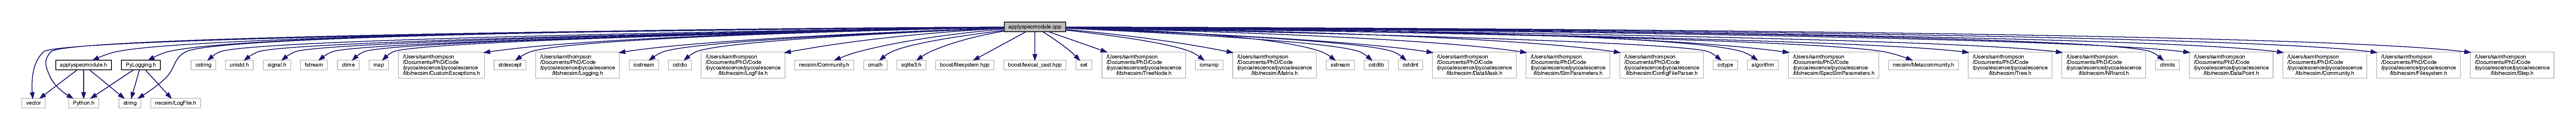
\includegraphics[width=350pt]{applyspecmodule_8cpp__incl}
\end{center}
\end{figure}
\subsection*{Macros}
\begin{DoxyCompactItemize}
\item 
\#define {\bfseries P\+Y\+T\+H\+O\+N\+\_\+\+C\+O\+M\+P\+I\+LE}\hypertarget{applyspecmodule_8cpp_a9302692bd9a9cf56478cbae301f04d53}{}\label{applyspecmodule_8cpp_a9302692bd9a9cf56478cbae301f04d53}

\item 
\#define {\bfseries I\+N\+I\+T\+E\+R\+R\+OR}~return\hypertarget{applyspecmodule_8cpp_a3d94077229c2876134769daeeb28fa8a}{}\label{applyspecmodule_8cpp_a3d94077229c2876134769daeeb28fa8a}

\end{DoxyCompactItemize}
\subsection*{Functions}
\begin{DoxyCompactItemize}
\item 
{\footnotesize template$<$class T $>$ }\\void \hyperlink{applyspecmodule_8cpp_ac7b006cc638258663ff8ebd5b55920e4}{create\+Community} (string database\+\_\+str, bool use\+\_\+spatial, string sample\+\_\+file, string time\+\_\+config\+\_\+file, string fragment\+\_\+file, vector$<$ double $>$ \&speciation\+\_\+rates, double min\+\_\+speciation\+\_\+gen, double max\+\_\+speciation\+\_\+gen, unsigned long metacommunity\+\_\+size, double metacommunity\+\_\+speciation\+\_\+rate)
\begin{DoxyCompactList}\small\item\em Applies the speciation parameters to the provided template class, which can be a \hyperlink{class_metacommunity}{Metacommunity} or a \hyperlink{class_community}{Community}. \end{DoxyCompactList}\item 
Py\+M\+O\+D\+I\+N\+I\+T\+\_\+\+F\+U\+NC {\bfseries initapplyspecmodule} (void)\hypertarget{applyspecmodule_8cpp_a1d49241e65981fb4ceca59a7e420decf}{}\label{applyspecmodule_8cpp_a1d49241e65981fb4ceca59a7e420decf}

\end{DoxyCompactItemize}
\subsection*{Variables}
\begin{DoxyCompactItemize}
\item 
Py\+Object $\ast$ {\bfseries loggingmodule}\hypertarget{applyspecmodule_8cpp_ae269920327ad06583db48e0bb122605e}{}\label{applyspecmodule_8cpp_ae269920327ad06583db48e0bb122605e}

\item 
Py\+G\+I\+L\+State\+\_\+\+S\+T\+A\+TE {\bfseries gstate}\hypertarget{applyspecmodule_8cpp_ae2ea2c066f7e65f192b08f50adb4ad1d}{}\label{applyspecmodule_8cpp_ae2ea2c066f7e65f192b08f50adb4ad1d}

\item 
bool {\bfseries log\+\_\+set} = false\hypertarget{applyspecmodule_8cpp_a304b2017ec52852821aced29cb2fe2ed}{}\label{applyspecmodule_8cpp_a304b2017ec52852821aced29cb2fe2ed}

\item 
bool {\bfseries logger\+\_\+set} = false\hypertarget{applyspecmodule_8cpp_a08d9fbb3de64e2e37d485a6fb7c413c9}{}\label{applyspecmodule_8cpp_a08d9fbb3de64e2e37d485a6fb7c413c9}

\item 
Py\+Object $\ast$ \hyperlink{applyspecmodule_8cpp_ac5c8cc1b55a6d2753d51817bd568aada}{logger}\hypertarget{applyspecmodule_8cpp_ac5c8cc1b55a6d2753d51817bd568aada}{}\label{applyspecmodule_8cpp_ac5c8cc1b55a6d2753d51817bd568aada}

\begin{DoxyCompactList}\small\item\em A python object container for the logger object for outputting using python\textquotesingle{}s logging module. \end{DoxyCompactList}\end{DoxyCompactItemize}


\subsection{Detailed Description}
Contains the module for python integration for additional applying speciation rates after a simulation is completed. 

\begin{DoxyAuthor}{Author}
Samuel Thompson 
\end{DoxyAuthor}
\begin{DoxyDate}{Date}
01/08/2017
\end{DoxyDate}
\begin{DoxyCopyright}{Copyright}
\href{https://opensource.org/licenses/BSD-3-Clause}{\tt B\+S\+D-\/3 Licence.} Requires command line parameters and generates a data object from them. Contact\+: \href{mailto:samuel.thompson14@imperial.ac.uk}{\tt samuel.\+thompson14@imperial.\+ac.\+uk} or \href{mailto:thompsonsed@gmail.com}{\tt thompsonsed@gmail.\+com} 
\end{DoxyCopyright}


\subsection{Function Documentation}
\index{applyspecmodule.\+cpp@{applyspecmodule.\+cpp}!create\+Community@{create\+Community}}
\index{create\+Community@{create\+Community}!applyspecmodule.\+cpp@{applyspecmodule.\+cpp}}
\subsubsection[{\texorpdfstring{create\+Community(string database\+\_\+str, bool use\+\_\+spatial, string sample\+\_\+file, string time\+\_\+config\+\_\+file, string fragment\+\_\+file, vector$<$ double $>$ \&speciation\+\_\+rates, double min\+\_\+speciation\+\_\+gen, double max\+\_\+speciation\+\_\+gen, unsigned long metacommunity\+\_\+size, double metacommunity\+\_\+speciation\+\_\+rate)}{createCommunity(string database_str, bool use_spatial, string sample_file, string time_config_file, string fragment_file, vector< double > &speciation_rates, double min_speciation_gen, double max_speciation_gen, unsigned long metacommunity_size, double metacommunity_speciation_rate)}}]{\setlength{\rightskip}{0pt plus 5cm}template$<$class T $>$ void create\+Community (
\begin{DoxyParamCaption}
\item[{string}]{database\+\_\+str, }
\item[{bool}]{use\+\_\+spatial, }
\item[{string}]{sample\+\_\+file, }
\item[{string}]{time\+\_\+config\+\_\+file, }
\item[{string}]{fragment\+\_\+file, }
\item[{vector$<$ double $>$ \&}]{speciation\+\_\+rates, }
\item[{double}]{min\+\_\+speciation\+\_\+gen, }
\item[{double}]{max\+\_\+speciation\+\_\+gen, }
\item[{unsigned long}]{metacommunity\+\_\+size, }
\item[{double}]{metacommunity\+\_\+speciation\+\_\+rate}
\end{DoxyParamCaption}
)}\hypertarget{applyspecmodule_8cpp_ac7b006cc638258663ff8ebd5b55920e4}{}\label{applyspecmodule_8cpp_ac7b006cc638258663ff8ebd5b55920e4}


Applies the speciation parameters to the provided template class, which can be a \hyperlink{class_metacommunity}{Metacommunity} or a \hyperlink{class_community}{Community}. 


\begin{DoxyTemplParams}{Template Parameters}
{\em T} & either a \hyperlink{class_metacommunity}{Metacommunity} of \hyperlink{class_community}{Community} object to calculate community structure for \\
\hline
\end{DoxyTemplParams}

\begin{DoxyParams}{Parameters}
{\em database\+\_\+str} & path to the database input/output \\
\hline
{\em use\+\_\+spatial} & flag for lineage location analysis \\
\hline
{\em sample\+\_\+file} & path to spatial sampling file, or \char`\"{}null\char`\"{} \\
\hline
{\em time\+\_\+config\+\_\+file} & path to temporal sampling file, or \char`\"{}null\char`\"{} \\
\hline
{\em fragment\+\_\+file} & path to fragment list, or \char`\"{}\+T\char`\"{} for fragment detection, or \char`\"{}null\char`\"{} \\
\hline
{\em speciation\+\_\+rates} & speciation rates to apply \\
\hline
{\em min\+\_\+speciation\+\_\+gen} & minimum speciation rate for protracted simulations \\
\hline
{\em max\+\_\+speciation\+\_\+gen} & maximum speciation rate for protracted simulations \\
\hline
{\em metacommunity\+\_\+size} & size of the metacommunity to apply \\
\hline
{\em metacommunity\+\_\+speciation\+\_\+rate} & speciation rate to use in metacommunity generation \\
\hline
\end{DoxyParams}

\hypertarget{applyspecmodule_8h}{}\section{applyspecmodule.\+h File Reference}
\label{applyspecmodule_8h}\index{applyspecmodule.\+h@{applyspecmodule.\+h}}


Contains the module for python integration for additional applying speciation rates after a simulation is completed.  


{\ttfamily \#include $<$Python.\+h$>$}\\*
{\ttfamily \#include $<$vector$>$}\\*
{\ttfamily \#include $<$string$>$}\\*
{\ttfamily \#include \char`\"{}Apply\+Spec.\+h\char`\"{}}\\*
{\ttfamily \#include \char`\"{}Logging.\+h\char`\"{}}\\*
Include dependency graph for applyspecmodule.\+h\+:
% FIG 0
This graph shows which files directly or indirectly include this file\+:
% FIG 1
\subsection*{Classes}
\begin{DoxyCompactItemize}
\item 
struct \hyperlink{structmodule__state}{module\+\_\+state}
\end{DoxyCompactItemize}
\subsection*{Macros}
\begin{DoxyCompactItemize}
\item 
\#define {\bfseries A\+P\+P\+L\+Y\+\_\+\+S\+P\+E\+C\+\_\+\+I\+M\+P\+O\+RT}\hypertarget{applyspecmodule_8h_acb552735854a92b373d5c9c832ca1219}{}\label{applyspecmodule_8h_acb552735854a92b373d5c9c832ca1219}

\item 
\#define {\bfseries G\+E\+T\+S\+T\+A\+TE}(m)~(\&\+\_\+state)\hypertarget{applyspecmodule_8h_a6d1f389576656b98c42c69f7cf1d55c0}{}\label{applyspecmodule_8h_a6d1f389576656b98c42c69f7cf1d55c0}

\item 
\#define {\bfseries I\+N\+I\+T\+E\+R\+R\+OR}~return\hypertarget{applyspecmodule_8h_a3d94077229c2876134769daeeb28fa8a}{}\label{applyspecmodule_8h_a3d94077229c2876134769daeeb28fa8a}

\end{DoxyCompactItemize}
\subsection*{Functions}
\begin{DoxyCompactItemize}
\item 
Py\+M\+O\+D\+I\+N\+I\+T\+\_\+\+F\+U\+NC {\bfseries initapplyspecmodule} (void)\hypertarget{applyspecmodule_8h_a1d49241e65981fb4ceca59a7e420decf}{}\label{applyspecmodule_8h_a1d49241e65981fb4ceca59a7e420decf}

\end{DoxyCompactItemize}


\subsection{Detailed Description}
Contains the module for python integration for additional applying speciation rates after a simulation is completed. 

\begin{DoxyAuthor}{Author}
Samuel Thompson 
\end{DoxyAuthor}
\begin{DoxyDate}{Date}
01/08/2017
\end{DoxyDate}
\begin{DoxyVersion}{Version}
1.\+0 
\end{DoxyVersion}
\begin{DoxyCopyright}{Copyright}
\href{https://opensource.org/licenses/BSD-3-Clause}{\tt B\+S\+D-\/3 Licence.} For use on the S\+QL database outputs of N\+E\+C\+Sim v3.\+1+. It requires command line parameters and generates a data object from them. Contact\+: \href{mailto:samuel.thompson14@imperial.ac.uk}{\tt samuel.\+thompson14@imperial.\+ac.\+uk} or \href{mailto:thompsonsed@gmail.com}{\tt thompsonsed@gmail.\+com} 
\end{DoxyCopyright}

\hypertarget{_custom_exceptions_8h}{}\section{Custom\+Exceptions.\+h File Reference}
\label{_custom_exceptions_8h}\index{Custom\+Exceptions.\+h@{Custom\+Exceptions.\+h}}


Contains the various exceptions used by N\+E\+C\+Sim.  


{\ttfamily \#include $<$stdexcept$>$}\\*
Include dependency graph for Custom\+Exceptions.\+h\+:
% FIG 0
This graph shows which files directly or indirectly include this file\+:
% FIG 1
\subsection*{Classes}
\begin{DoxyCompactItemize}
\item 
struct \hyperlink{struct_main___exception}{Main\+\_\+\+Exception}
\begin{DoxyCompactList}\small\item\em These are used for non-\/fatal exception thrown from within the main simulation where no-\/more specific location information is possible. \end{DoxyCompactList}\item 
struct \hyperlink{struct_fatal___exception}{Fatal\+\_\+\+Exception}
\begin{DoxyCompactList}\small\item\em This is called any time a fatal exception is called and the program is unwound and ended. \end{DoxyCompactList}\item 
struct \hyperlink{struct_map___exception}{Map\+\_\+\+Exception}
\begin{DoxyCompactList}\small\item\em The non-\/fatal exception thrown when a problem is encountered in any \hyperlink{class_map}{Map} object processes. \end{DoxyCompactList}\item 
struct \hyperlink{struct_map___fatal___exception}{Map\+\_\+\+Fatal\+\_\+\+Exception}
\begin{DoxyCompactList}\small\item\em The fatal exception thrown when a problem is encountered in any \hyperlink{class_map}{Map} object processes. \end{DoxyCompactList}\item 
struct \hyperlink{struct_config___exception}{Config\+\_\+\+Exception}
\begin{DoxyCompactList}\small\item\em A structure for all exceptions thrown within config processes. \end{DoxyCompactList}\item 
struct \hyperlink{struct_species_exception}{Species\+Exception}
\begin{DoxyCompactList}\small\item\em An exception thrown whenever a non-\/fatal Species exception is thrown. \end{DoxyCompactList}\end{DoxyCompactItemize}


\subsection{Detailed Description}
Contains the various exceptions used by N\+E\+C\+Sim. 

\begin{DoxyAuthor}{Author}
Samuel Thompson
\end{DoxyAuthor}
\begin{DoxyCopyright}{Copyright}
\href{https://opensource.org/licenses/BSD-3-Clause}{\tt B\+S\+D-\/3 Licence.} 
\end{DoxyCopyright}

\hypertarget{_datapoint_8h}{}\section{Datapoint.\+h File Reference}
\label{_datapoint_8h}\index{Datapoint.\+h@{Datapoint.\+h}}


Contains the \hyperlink{class_datapoint}{Datapoint} class for storing objects during simulation run time.  


{\ttfamily \#include $<$iostream$>$}\\*
{\ttfamily \#include \char`\"{}Logging.\+h\char`\"{}}\\*
Include dependency graph for Datapoint.\+h\+:
% FIG 0
This graph shows which files directly or indirectly include this file\+:
% FIG 1
\subsection*{Classes}
\begin{DoxyCompactItemize}
\item 
class \hyperlink{class_datapoint}{Datapoint}
\begin{DoxyCompactList}\small\item\em A data object used in coalescence simulations for calculating the output. Data from this object is outputted to an S\+Q\+Lite database after simulations are complete. \end{DoxyCompactList}\end{DoxyCompactItemize}


\subsection{Detailed Description}
Contains the \hyperlink{class_datapoint}{Datapoint} class for storing objects during simulation run time. 

\begin{DoxyAuthor}{Author}
Samuel Thompson 
\end{DoxyAuthor}
\begin{DoxyDate}{Date}
30/08/2016
\end{DoxyDate}
\begin{DoxyVersion}{Version}
2.\+01 
\end{DoxyVersion}
\begin{DoxyCopyright}{Copyright}
\href{https://opensource.org/licenses/BSD-3-Clause}{\tt B\+S\+D-\/3 Licence.} This class is only used during simulation runs and is not outputted to a database. A \hyperlink{class_row}{Row} of \hyperlink{class_datapoint}{Datapoint} objects is utilised by the main \hyperlink{class_tree}{CoalescenceTree} objects.
\end{DoxyCopyright}

\hypertarget{_dispersal_coordinator_8cpp}{}\section{Dispersal\+Coordinator.\+cpp File Reference}
\label{_dispersal_coordinator_8cpp}\index{Dispersal\+Coordinator.\+cpp@{Dispersal\+Coordinator.\+cpp}}


Contains the \hyperlink{class_dispersal_coordinator}{Dispersal\+Coordinator}, which contains all routines related to dispersal including utilisation of density maps and dispersal probability maps.  


{\ttfamily \#include \char`\"{}Dispersal\+Coordinator.\+h\char`\"{}}\\*
Include dependency graph for Dispersal\+Coordinator.\+cpp\+:
% FIG 0


\subsection{Detailed Description}
Contains the \hyperlink{class_dispersal_coordinator}{Dispersal\+Coordinator}, which contains all routines related to dispersal including utilisation of density maps and dispersal probability maps. 

\begin{DoxyAuthor}{Author}
Samuel Thompson 
\end{DoxyAuthor}
\begin{DoxyDate}{Date}
07/08/2017
\end{DoxyDate}
\begin{DoxyCopyright}{Copyright}
\href{https://opensource.org/licenses/BSD-3-Clause}{\tt B\+S\+D-\/3 Licence.} 
\end{DoxyCopyright}

\hypertarget{_dispersal_coordinator_8h}{}\section{necsim/\+Dispersal\+Coordinator.h File Reference}
\label{_dispersal_coordinator_8h}\index{necsim/\+Dispersal\+Coordinator.\+h@{necsim/\+Dispersal\+Coordinator.\+h}}


Contains the \hyperlink{class_dispersal_coordinator}{Dispersal\+Coordinator}, which contains all routines related to dispersal including utilisation of density maps and dispersal probability maps.  


{\ttfamily \#include $<$cstring$>$}\\*
{\ttfamily \#include $<$cstdio$>$}\\*
{\ttfamily \#include $<$iostream$>$}\\*
{\ttfamily \#include $<$fstream$>$}\\*
{\ttfamily \#include $<$stdexcept$>$}\\*
{\ttfamily \#include $<$cmath$>$}\\*
{\ttfamily \#include \char`\"{}N\+Rrand.\+h\char`\"{}}\\*
{\ttfamily \#include \char`\"{}Matrix.\+h\char`\"{}}\\*
{\ttfamily \#include \char`\"{}Step.\+h\char`\"{}}\\*
{\ttfamily \#include \char`\"{}Map.\+h\char`\"{}}\\*
Include dependency graph for Dispersal\+Coordinator.\+h\+:\nopagebreak
\begin{figure}[H]
\begin{center}
\leavevmode
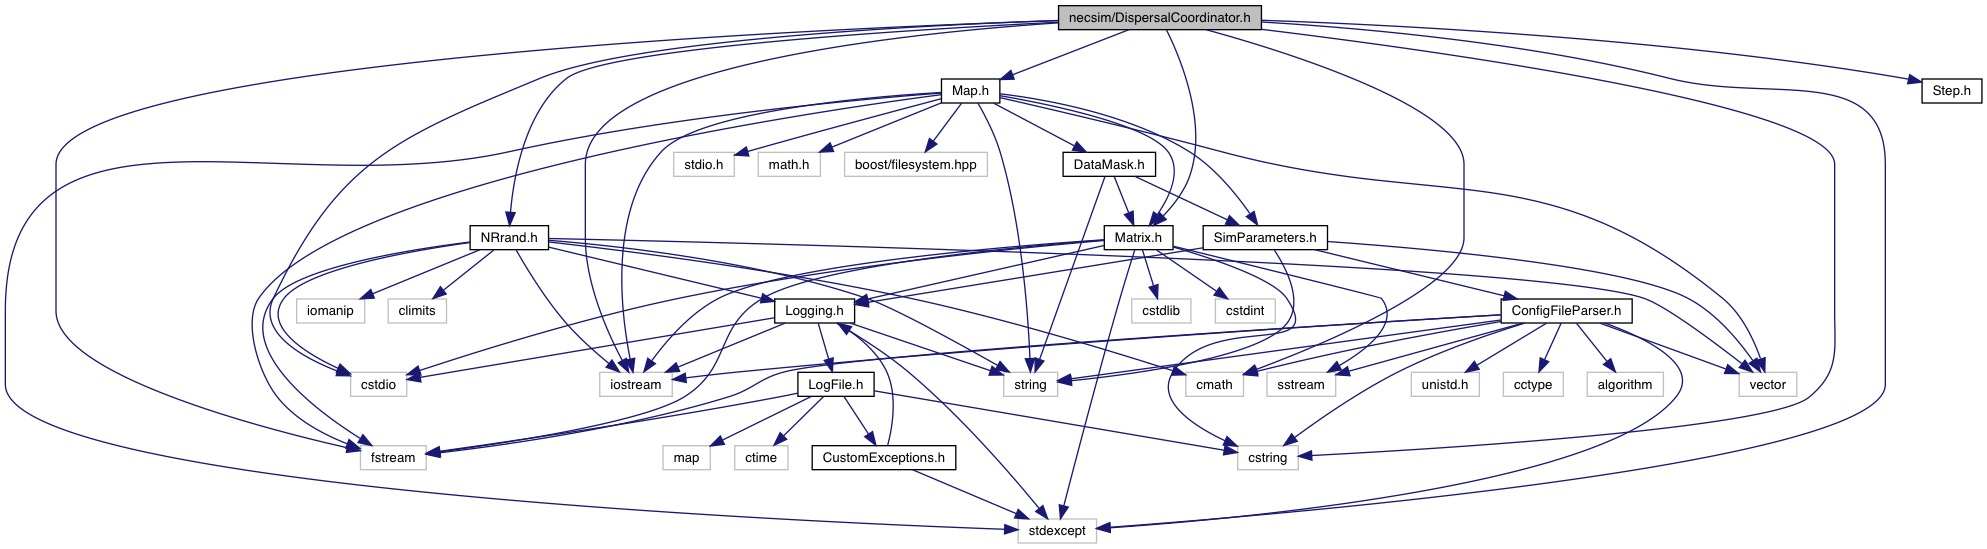
\includegraphics[width=350pt]{_dispersal_coordinator_8h__incl}
\end{center}
\end{figure}
This graph shows which files directly or indirectly include this file\+:\nopagebreak
\begin{figure}[H]
\begin{center}
\leavevmode
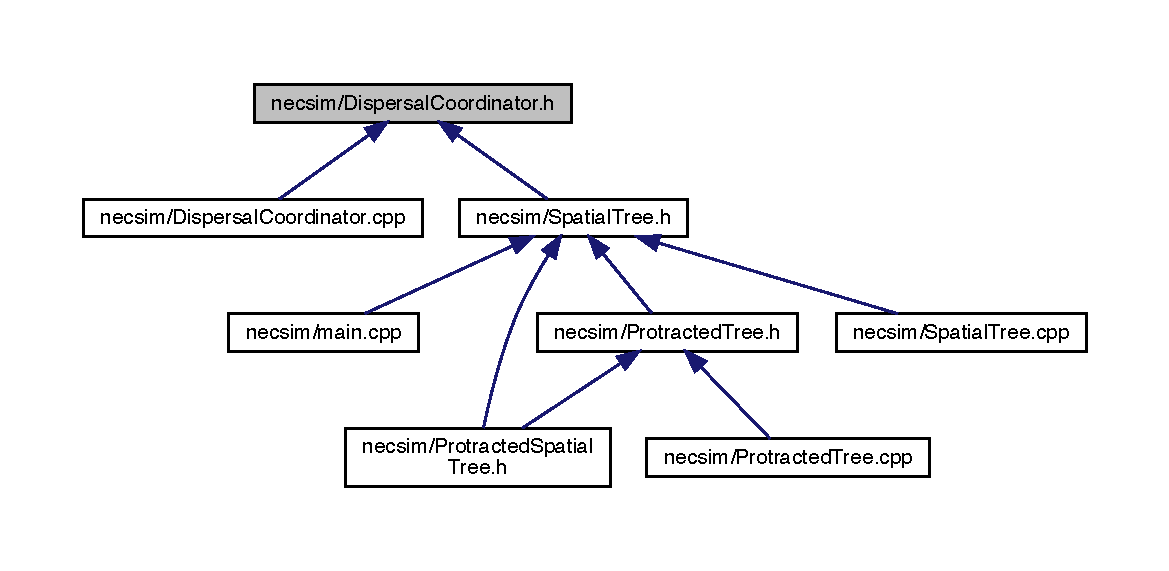
\includegraphics[width=350pt]{_dispersal_coordinator_8h__dep__incl}
\end{center}
\end{figure}
\subsection*{Classes}
\begin{DoxyCompactItemize}
\item 
class \hyperlink{class_dispersal_coordinator}{Dispersal\+Coordinator}
\begin{DoxyCompactList}\small\item\em Class for generating dispersal distances and provide routines for reading dispersal distance maps as a unwound map-\/of-\/maps. This class also handles reading density maps for rejection sampling. \end{DoxyCompactList}\end{DoxyCompactItemize}


\subsection{Detailed Description}
Contains the \hyperlink{class_dispersal_coordinator}{Dispersal\+Coordinator}, which contains all routines related to dispersal including utilisation of density maps and dispersal probability maps. 

\begin{DoxyAuthor}{Author}
Samuel Thompson 
\end{DoxyAuthor}
\begin{DoxyDate}{Date}
07/08/2017
\end{DoxyDate}
\begin{DoxyCopyright}{Copyright}
\href{https://opensource.org/licenses/BSD-3-Clause}{\tt B\+S\+D-\/3 Licence.} 
\end{DoxyCopyright}

\hypertarget{dispersalmodule_8cpp}{}\section{dispersalmodule.\+cpp File Reference}
\label{dispersalmodule_8cpp}\index{dispersalmodule.\+cpp@{dispersalmodule.\+cpp}}


Contains the functions for testing dispersal methods using efficient c++ routines.  


{\ttfamily \#include $<$Python.\+h$>$}\\*
{\ttfamily \#include $<$vector$>$}\\*
{\ttfamily \#include $<$string$>$}\\*
{\ttfamily \#include $<$cstring$>$}\\*
{\ttfamily \#include $<$unistd.\+h$>$}\\*
{\ttfamily \#include $<$signal.\+h$>$}\\*
{\ttfamily \#include \char`\"{}dispersalmodule.\+h\char`\"{}}\\*
Include dependency graph for dispersalmodule.\+cpp\+:
% FIG 0
\subsection*{Macros}
\begin{DoxyCompactItemize}
\item 
\#define {\bfseries P\+Y\+T\+H\+O\+N\+\_\+\+C\+O\+M\+P\+I\+LE}\hypertarget{dispersalmodule_8cpp_a9302692bd9a9cf56478cbae301f04d53}{}\label{dispersalmodule_8cpp_a9302692bd9a9cf56478cbae301f04d53}

\item 
\#define {\bfseries I\+N\+I\+T\+E\+R\+R\+OR}~return\hypertarget{dispersalmodule_8cpp_a3d94077229c2876134769daeeb28fa8a}{}\label{dispersalmodule_8cpp_a3d94077229c2876134769daeeb28fa8a}

\end{DoxyCompactItemize}
\subsection*{Functions}
\begin{DoxyCompactItemize}
\item 
Py\+M\+O\+D\+I\+N\+I\+T\+\_\+\+F\+U\+NC {\bfseries initdispersalmodule} (void)\hypertarget{dispersalmodule_8cpp_a6bb4c0faf0e3fd0b77bbad879dfec993}{}\label{dispersalmodule_8cpp_a6bb4c0faf0e3fd0b77bbad879dfec993}

\end{DoxyCompactItemize}
\subsection*{Variables}
\begin{DoxyCompactItemize}
\item 
Py\+Object $\ast$ {\bfseries loggingmodule}\hypertarget{dispersalmodule_8cpp_ae269920327ad06583db48e0bb122605e}{}\label{dispersalmodule_8cpp_ae269920327ad06583db48e0bb122605e}

\item 
Py\+G\+I\+L\+State\+\_\+\+S\+T\+A\+TE {\bfseries gstate}\hypertarget{dispersalmodule_8cpp_ae2ea2c066f7e65f192b08f50adb4ad1d}{}\label{dispersalmodule_8cpp_ae2ea2c066f7e65f192b08f50adb4ad1d}

\item 
bool {\bfseries log\+\_\+set} = false\hypertarget{dispersalmodule_8cpp_a304b2017ec52852821aced29cb2fe2ed}{}\label{dispersalmodule_8cpp_a304b2017ec52852821aced29cb2fe2ed}

\item 
bool {\bfseries logger\+\_\+set} = false\hypertarget{dispersalmodule_8cpp_a08d9fbb3de64e2e37d485a6fb7c413c9}{}\label{dispersalmodule_8cpp_a08d9fbb3de64e2e37d485a6fb7c413c9}

\item 
Py\+Object $\ast$ {\bfseries logger}\hypertarget{dispersalmodule_8cpp_ac5c8cc1b55a6d2753d51817bd568aada}{}\label{dispersalmodule_8cpp_ac5c8cc1b55a6d2753d51817bd568aada}

\end{DoxyCompactItemize}


\subsection{Detailed Description}
Contains the functions for testing dispersal methods using efficient c++ routines. 

\begin{DoxyAuthor}{Author}
Samuel Thompson
\end{DoxyAuthor}
\begin{DoxyCopyright}{Copyright}
\href{https://opensource.org/licenses/BSD-3-Clause}{\tt B\+S\+D-\/3 Licence.} 
\end{DoxyCopyright}

\hypertarget{dispersalmodule_8h}{}\section{dispersalmodule.\+h File Reference}
\label{dispersalmodule_8h}\index{dispersalmodule.\+h@{dispersalmodule.\+h}}


Contains the functions for testing dispersal methods using efficient c++ routines.  


{\ttfamily \#include $<$Python.\+h$>$}\\*
{\ttfamily \#include $<$vector$>$}\\*
{\ttfamily \#include $<$string$>$}\\*
Include dependency graph for dispersalmodule.\+h\+:\nopagebreak
\begin{figure}[H]
\begin{center}
\leavevmode
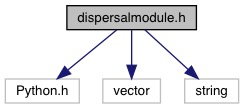
\includegraphics[width=255pt]{dispersalmodule_8h__incl}
\end{center}
\end{figure}
This graph shows which files directly or indirectly include this file\+:\nopagebreak
\begin{figure}[H]
\begin{center}
\leavevmode
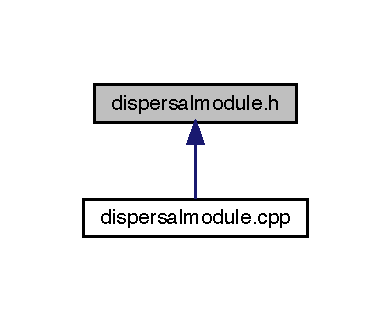
\includegraphics[width=188pt]{dispersalmodule_8h__dep__incl}
\end{center}
\end{figure}
\subsection*{Classes}
\begin{DoxyCompactItemize}
\item 
struct \hyperlink{structmodule__state}{module\+\_\+state}
\end{DoxyCompactItemize}
\subsection*{Macros}
\begin{DoxyCompactItemize}
\item 
\#define {\bfseries D\+I\+S\+P\+E\+R\+S\+A\+L\+\_\+\+I\+M\+P\+O\+RT}\hypertarget{dispersalmodule_8h_a11c30aa5aed370a0aa25f1f735501459}{}\label{dispersalmodule_8h_a11c30aa5aed370a0aa25f1f735501459}

\item 
\#define {\bfseries G\+E\+T\+S\+T\+A\+TE}(m)~(\&\+\_\+state)\hypertarget{dispersalmodule_8h_a6d1f389576656b98c42c69f7cf1d55c0}{}\label{dispersalmodule_8h_a6d1f389576656b98c42c69f7cf1d55c0}

\item 
\#define {\bfseries I\+N\+I\+T\+E\+R\+R\+OR}~return\hypertarget{dispersalmodule_8h_a3d94077229c2876134769daeeb28fa8a}{}\label{dispersalmodule_8h_a3d94077229c2876134769daeeb28fa8a}

\end{DoxyCompactItemize}
\subsection*{Functions}
\begin{DoxyCompactItemize}
\item 
Py\+M\+O\+D\+I\+N\+I\+T\+\_\+\+F\+U\+NC {\bfseries initdispersalmodule} (void)\hypertarget{dispersalmodule_8h_a6bb4c0faf0e3fd0b77bbad879dfec993}{}\label{dispersalmodule_8h_a6bb4c0faf0e3fd0b77bbad879dfec993}

\end{DoxyCompactItemize}


\subsection{Detailed Description}
Contains the functions for testing dispersal methods using efficient c++ routines. 

\begin{DoxyAuthor}{Author}
Samuel Thompson
\end{DoxyAuthor}
\begin{DoxyCopyright}{Copyright}
\href{https://opensource.org/licenses/BSD-3-Clause}{\tt B\+S\+D-\/3 Licence.} 
\end{DoxyCopyright}

\hypertarget{_fattaildeviate_8h}{}\section{Fattaildeviate.\+h File Reference}
\label{_fattaildeviate_8h}\index{Fattaildeviate.\+h@{Fattaildeviate.\+h}}


Contains a generic random number generator. Provided by James Rosindell (\href{mailto:j.rosindell@imperial.ac.uk}{\tt j.\+rosindell@imperial.\+ac.\+uk}) with moderate modifications by Samuel Thompson (\href{mailto:thomsonsed@gmail.com}{\tt thomsonsed@gmail.\+com}).  


{\ttfamily \#include $<$stdio.\+h$>$}\\*
{\ttfamily \#include $<$string$>$}\\*
{\ttfamily \#include $<$iomanip$>$}\\*
{\ttfamily \#include $<$math.\+h$>$}\\*
{\ttfamily \#include $<$vector$>$}\\*
{\ttfamily \#include $<$iostream$>$}\\*
{\ttfamily \#include $<$fstream$>$}\\*
{\ttfamily \#include \char`\"{}Logging.\+h\char`\"{}}\\*
Include dependency graph for Fattaildeviate.\+h\+:
% FIG 0
This graph shows which files directly or indirectly include this file\+:
% FIG 1
\subsection*{Classes}
\begin{DoxyCompactItemize}
\item 
class \hyperlink{class_n_rrand}{N\+Rrand}
\begin{DoxyCompactList}\small\item\em Contains the functions for random number generation. \end{DoxyCompactList}\end{DoxyCompactItemize}
\subsection*{Macros}
\begin{DoxyCompactItemize}
\item 
\#define {\bfseries I\+M1}~2147483563\hypertarget{_fattaildeviate_8h_a78325bdf48423acef7c012567628b391}{}\label{_fattaildeviate_8h_a78325bdf48423acef7c012567628b391}

\item 
\#define {\bfseries I\+M2}~2147483399\hypertarget{_fattaildeviate_8h_ad8c519de7e5de4ae35344ddcf21fd062}{}\label{_fattaildeviate_8h_ad8c519de7e5de4ae35344ddcf21fd062}

\item 
\#define {\bfseries AM}~(1.\+0/I\+M1)\hypertarget{_fattaildeviate_8h_ad301e6a88b1c01108f4867f2ea6f683c}{}\label{_fattaildeviate_8h_ad301e6a88b1c01108f4867f2ea6f683c}

\item 
\#define {\bfseries I\+M\+M1}~(I\+M1-\/1)\hypertarget{_fattaildeviate_8h_a87a6e0054f9d827c979c43aa0d5e621a}{}\label{_fattaildeviate_8h_a87a6e0054f9d827c979c43aa0d5e621a}

\item 
\#define {\bfseries I\+A1}~40014\hypertarget{_fattaildeviate_8h_a6ef2749dca39c605c3d033f788afe6e3}{}\label{_fattaildeviate_8h_a6ef2749dca39c605c3d033f788afe6e3}

\item 
\#define {\bfseries I\+A2}~40692\hypertarget{_fattaildeviate_8h_a372a58d7e9e25912fd79e7afaa06cc7a}{}\label{_fattaildeviate_8h_a372a58d7e9e25912fd79e7afaa06cc7a}

\item 
\#define {\bfseries I\+Q1}~53668\hypertarget{_fattaildeviate_8h_a9afa86ff22da69bda72fe271ae71ad46}{}\label{_fattaildeviate_8h_a9afa86ff22da69bda72fe271ae71ad46}

\item 
\#define {\bfseries I\+Q2}~5277\hypertarget{_fattaildeviate_8h_abae040385946a6acdf5e10d2efd86f3d}{}\label{_fattaildeviate_8h_abae040385946a6acdf5e10d2efd86f3d}

\item 
\#define {\bfseries I\+R1}~12211\hypertarget{_fattaildeviate_8h_a7b2b32709f9770a283701ffcf3723497}{}\label{_fattaildeviate_8h_a7b2b32709f9770a283701ffcf3723497}

\item 
\#define {\bfseries I\+R2}~3791\hypertarget{_fattaildeviate_8h_a5a08e4f5cb3582e623cc14a6c92d48de}{}\label{_fattaildeviate_8h_a5a08e4f5cb3582e623cc14a6c92d48de}

\item 
\#define {\bfseries N\+T\+AB}~32\hypertarget{_fattaildeviate_8h_a0e93cfb2d62849853fd34957ba6e6fdc}{}\label{_fattaildeviate_8h_a0e93cfb2d62849853fd34957ba6e6fdc}

\item 
\#define {\bfseries N\+D\+IV}~(1+I\+M\+M1/N\+T\+AB)\hypertarget{_fattaildeviate_8h_a62339d74dd5d9d00480e1a288cf88fe8}{}\label{_fattaildeviate_8h_a62339d74dd5d9d00480e1a288cf88fe8}

\item 
\#define {\bfseries E\+PS}~1.\+2e-\/8\hypertarget{_fattaildeviate_8h_a6ebf6899d6c1c8b7b9d09be872c05aae}{}\label{_fattaildeviate_8h_a6ebf6899d6c1c8b7b9d09be872c05aae}

\item 
\#define {\bfseries R\+N\+MX}~(1.\+0-\/E\+PS)\hypertarget{_fattaildeviate_8h_aa7436c9270ffb06f8c1eae8d2e605cec}{}\label{_fattaildeviate_8h_aa7436c9270ffb06f8c1eae8d2e605cec}

\end{DoxyCompactItemize}


\subsection{Detailed Description}
Contains a generic random number generator. Provided by James Rosindell (\href{mailto:j.rosindell@imperial.ac.uk}{\tt j.\+rosindell@imperial.\+ac.\+uk}) with moderate modifications by Samuel Thompson (\href{mailto:thomsonsed@gmail.com}{\tt thomsonsed@gmail.\+com}). 

\begin{DoxyAuthor}{Author}
James Rosindell 
\end{DoxyAuthor}
\begin{DoxyDate}{Date}
31/08/16
\end{DoxyDate}
The definitions for the constants defined here should not be altered. \begin{DoxyCopyright}{Copyright}
\href{https://opensource.org/licenses/BSD-3-Clause}{\tt B\+S\+D-\/3 Licence.} 
\end{DoxyCopyright}

\hypertarget{_logging_8cpp}{}\section{necsim/\+Logging.cpp File Reference}
\label{_logging_8cpp}\index{necsim/\+Logging.\+cpp@{necsim/\+Logging.\+cpp}}


Routines for writing to cout. Intended to be overloaded for pythonic versions with the logging module.  


{\ttfamily \#include $<$sstream$>$}\\*
{\ttfamily \#include \char`\"{}Logging.\+h\char`\"{}}\\*
Include dependency graph for Logging.\+cpp\+:\nopagebreak
\begin{figure}[H]
\begin{center}
\leavevmode
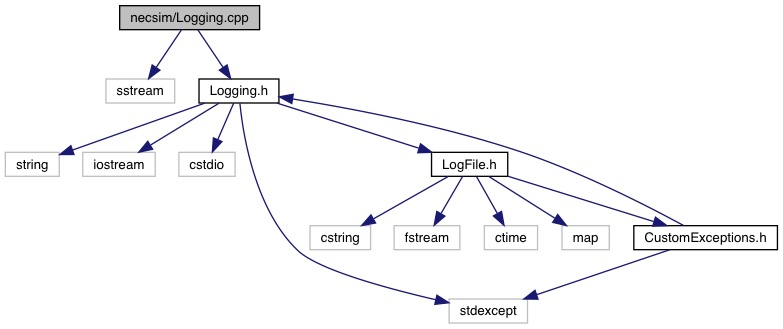
\includegraphics[width=350pt]{_logging_8cpp__incl}
\end{center}
\end{figure}
\subsection*{Functions}
\begin{DoxyCompactItemize}
\item 
void {\bfseries write\+Info} (string message)\hypertarget{_logging_8cpp_a4489578cda60bd87e9f634bc97ccfba1}{}\label{_logging_8cpp_a4489578cda60bd87e9f634bc97ccfba1}

\item 
void {\bfseries write\+Warning} (string message)\hypertarget{_logging_8cpp_ae911b2f9a56fe4054c9e72613eb73562}{}\label{_logging_8cpp_ae911b2f9a56fe4054c9e72613eb73562}

\item 
void {\bfseries write\+Error} (string message)\hypertarget{_logging_8cpp_a36370a5a1bc7559a8c29f35453158bb5}{}\label{_logging_8cpp_a36370a5a1bc7559a8c29f35453158bb5}

\item 
void {\bfseries write\+Critical} (string message)\hypertarget{_logging_8cpp_ae237237ebe013cbaa842ee6b43db15ba}{}\label{_logging_8cpp_ae237237ebe013cbaa842ee6b43db15ba}

\end{DoxyCompactItemize}


\subsection{Detailed Description}
Routines for writing to cout. Intended to be overloaded for pythonic versions with the logging module. 

\begin{DoxyAuthor}{Author}
Sam Thompson
\end{DoxyAuthor}
\begin{DoxyCopyright}{Copyright}
\href{https://opensource.org/licenses/BSD-3-Clause}{\tt B\+S\+D-\/3 Licence.} 
\end{DoxyCopyright}

\hypertarget{_logging_8h}{}\section{necsim/\+Logging.h File Reference}
\label{_logging_8h}\index{necsim/\+Logging.\+h@{necsim/\+Logging.\+h}}


Routines for writing to cout. Intended to be overloaded for pythonic versions with the logging module.  


{\ttfamily \#include $<$string$>$}\\*
{\ttfamily \#include $<$iostream$>$}\\*
{\ttfamily \#include $<$cstdio$>$}\\*
{\ttfamily \#include $<$stdexcept$>$}\\*
{\ttfamily \#include \char`\"{}Log\+File.\+h\char`\"{}}\\*
Include dependency graph for Logging.\+h\+:\nopagebreak
\begin{figure}[H]
\begin{center}
\leavevmode
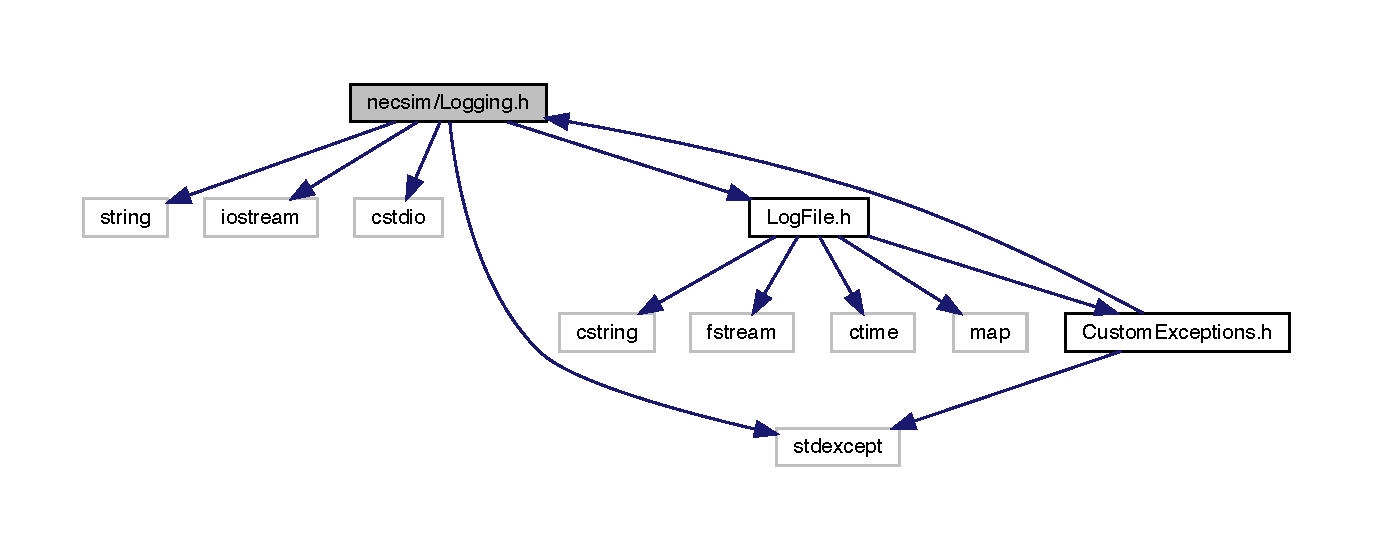
\includegraphics[width=350pt]{_logging_8h__incl}
\end{center}
\end{figure}
This graph shows which files directly or indirectly include this file\+:
\nopagebreak
\begin{figure}[H]
\begin{center}
\leavevmode
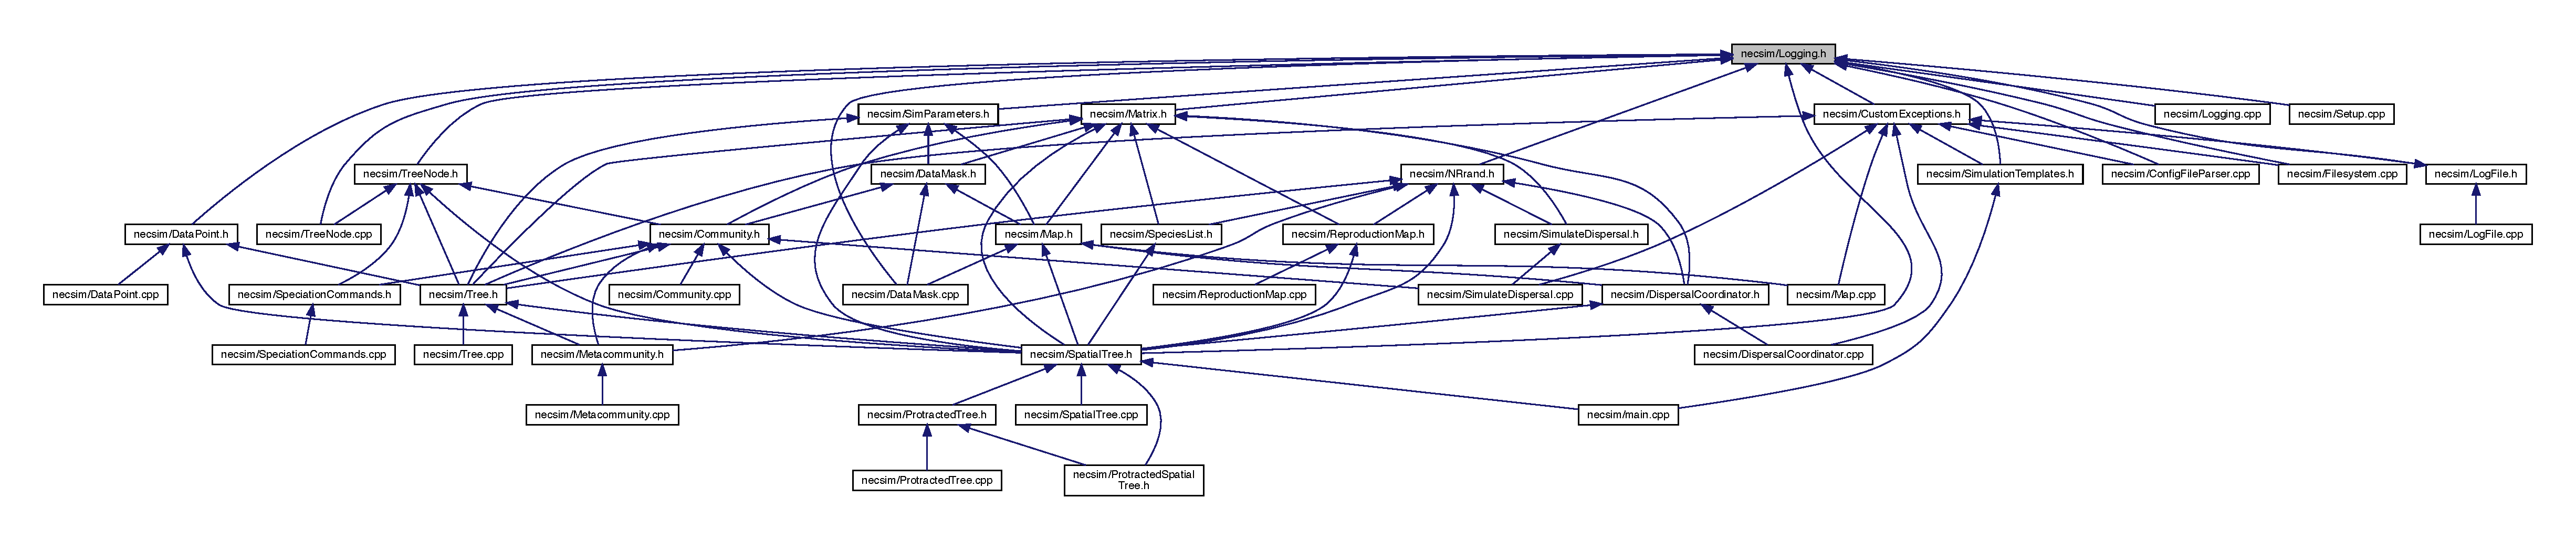
\includegraphics[width=350pt]{_logging_8h__dep__incl}
\end{center}
\end{figure}


\subsection{Detailed Description}
Routines for writing to cout. Intended to be overloaded for pythonic versions with the logging module. 

\begin{DoxyAuthor}{Author}
Sam Thompson
\end{DoxyAuthor}
\begin{DoxyCopyright}{Copyright}
\href{https://opensource.org/licenses/BSD-3-Clause}{\tt B\+S\+D-\/3 Licence.} 
\end{DoxyCopyright}

\hypertarget{main_8cpp}{}\section{main.\+cpp File Reference}
\label{main_8cpp}\index{main.\+cpp@{main.\+cpp}}


A generic simulator for spatially explicit coalescence models suitable for H\+PC applications. It contains all functions for running large-\/scale simulations backwards in time using coalescence techniques. Outputs include an S\+Q\+Lite database containing spatial and temporal information about tracked lineages, and allow for rebuilding of the coalescence tree. Currently, a fat-\/tailed dispersal kernel or normal distribution can be used for dispersal processes.  


{\ttfamily \#include $<$stdio.\+h$>$}\\*
{\ttfamily \#include \char`\"{}Setup.\+h\char`\"{}}\\*
Include dependency graph for main.\+cpp\+:
% FIG 0
\subsection*{Functions}
\begin{DoxyCompactItemize}
\item 
int \hyperlink{main_8cpp_a0ddf1224851353fc92bfbff6f499fa97}{main} (int argc, char $\ast$argv\mbox{[}$\,$\mbox{]})
\begin{DoxyCompactList}\small\item\em Main function containing program structure. \end{DoxyCompactList}\end{DoxyCompactItemize}


\subsection{Detailed Description}
A generic simulator for spatially explicit coalescence models suitable for H\+PC applications. It contains all functions for running large-\/scale simulations backwards in time using coalescence techniques. Outputs include an S\+Q\+Lite database containing spatial and temporal information about tracked lineages, and allow for rebuilding of the coalescence tree. Currently, a fat-\/tailed dispersal kernel or normal distribution can be used for dispersal processes. 

Run with -\/h to see full input options.

Outputs include
\begin{DoxyItemize}
\item habitat map file(s)
\item species richness and species abundances for the supplied minimum speciation rate.
\item S\+QL database containing full spatial data. This can be later analysed by the Speciation\+\_\+\+Counter program for applying higher speciation rates.
\end{DoxyItemize}

Contact\+: \href{mailto:samuel.thompson14@imperial.ac.uk}{\tt samuel.\+thompson14@imperial.\+ac.\+uk} or \href{mailto:thompsonsed@gmail.com}{\tt thompsonsed@gmail.\+com}

Based heavily on code written by James Rosindell

Contact\+: \href{mailto:j.rosindell@imperial.ac.uk}{\tt j.\+rosindell@imperial.\+ac.\+uk}

\begin{DoxyAuthor}{Author}
Samuel Thompson 
\end{DoxyAuthor}
\begin{DoxyVersion}{Version}
3.\+6 
\end{DoxyVersion}
\begin{DoxyCopyright}{Copyright}
\href{https://opensource.org/licenses/BSD-3-Clause}{\tt B\+S\+D-\/3 Licence.} 
\end{DoxyCopyright}


\subsection{Function Documentation}
\index{main.\+cpp@{main.\+cpp}!main@{main}}
\index{main@{main}!main.\+cpp@{main.\+cpp}}
\subsubsection[{\texorpdfstring{main(int argc, char $\ast$argv[])}{main(int argc, char *argv[])}}]{\setlength{\rightskip}{0pt plus 5cm}int main (
\begin{DoxyParamCaption}
\item[{int}]{argc, }
\item[{char $\ast$}]{argv\mbox{[}$\,$\mbox{]}}
\end{DoxyParamCaption}
)}\hypertarget{main_8cpp_a0ddf1224851353fc92bfbff6f499fa97}{}\label{main_8cpp_a0ddf1224851353fc92bfbff6f499fa97}


Main function containing program structure. 


\begin{DoxyParams}{Parameters}
{\em argc} & the number of command-\/line arguments provided \\
\hline
{\em argv} & a pointer to the arguments \\
\hline
\end{DoxyParams}
\begin{DoxyReturn}{Returns}
a program exit code, 0 if successful, -\/1 (generally) indicates an error. 
\end{DoxyReturn}

\hypertarget{_map_8cpp}{}\section{necsim/\+Map.cpp File Reference}
\label{_map_8cpp}\index{necsim/\+Map.\+cpp@{necsim/\+Map.\+cpp}}


Contains the \hyperlink{class_map}{Map} class implementation for easy referencing of the respective coarse and fine map within the same coordinate system.  


{\ttfamily \#include \char`\"{}Map.\+h\char`\"{}}\\*
{\ttfamily \#include \char`\"{}Filesystem.\+h\char`\"{}}\\*
{\ttfamily \#include \char`\"{}Custom\+Exceptions.\+h\char`\"{}}\\*
Include dependency graph for Map.\+cpp\+:\nopagebreak
\begin{figure}[H]
\begin{center}
\leavevmode
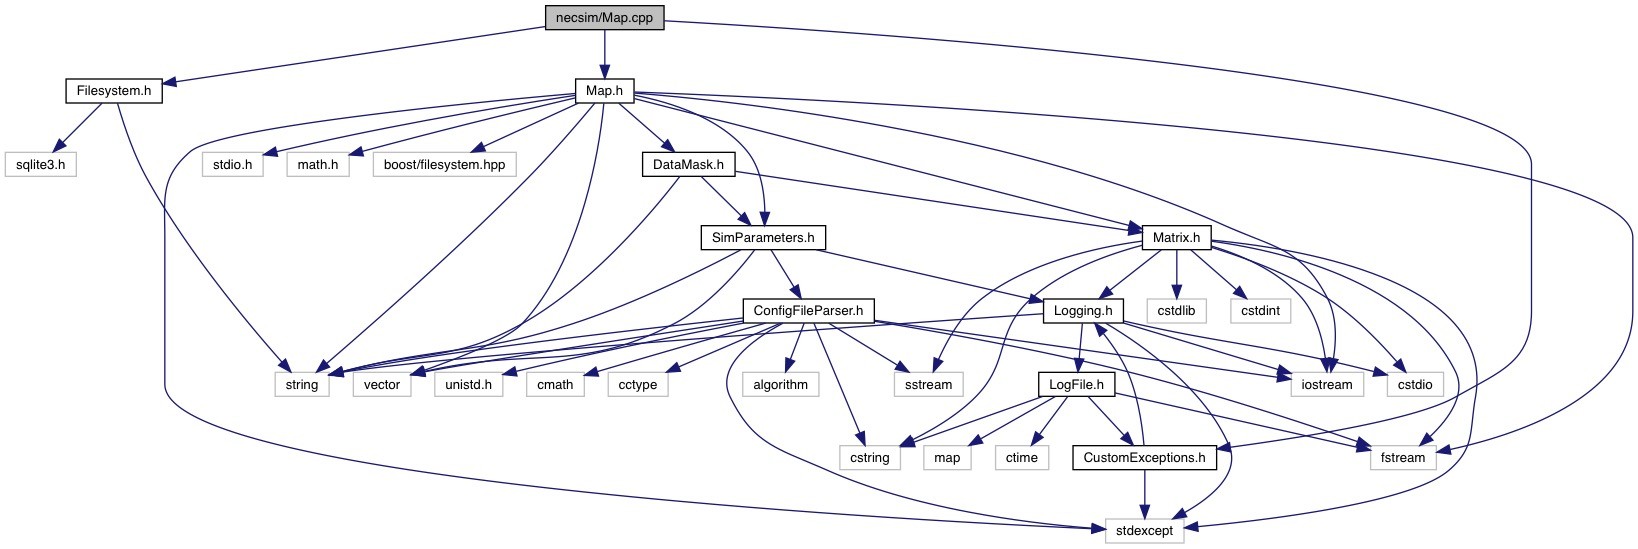
\includegraphics[width=350pt]{_map_8cpp__incl}
\end{center}
\end{figure}


\subsection{Detailed Description}
Contains the \hyperlink{class_map}{Map} class implementation for easy referencing of the respective coarse and fine map within the same coordinate system. 

\begin{DoxyAuthor}{Author}
Samuel Thompson
\end{DoxyAuthor}
\begin{DoxyCopyright}{Copyright}
\href{https://opensource.org/licenses/BSD-3-Clause}{\tt B\+S\+D-\/3 Licence.} 
\end{DoxyCopyright}

\hypertarget{_map_8h}{}\section{Map.\+h File Reference}
\label{_map_8h}\index{Map.\+h@{Map.\+h}}


Contains the \hyperlink{class_map}{Map} object for easy referencing of the respective coarse and fine map within the same coordinate system.  


{\ttfamily \#include $<$string$>$}\\*
{\ttfamily \#include $<$stdio.\+h$>$}\\*
{\ttfamily \#include $<$vector$>$}\\*
{\ttfamily \#include $<$iostream$>$}\\*
{\ttfamily \#include $<$fstream$>$}\\*
{\ttfamily \#include $<$math.\+h$>$}\\*
{\ttfamily \#include $<$stdexcept$>$}\\*
{\ttfamily \#include \char`\"{}Config\+File\+Parser.\+h\char`\"{}}\\*
{\ttfamily \#include $<$boost/filesystem.\+hpp$>$}\\*
{\ttfamily \#include \char`\"{}Matrix.\+h\char`\"{}}\\*
{\ttfamily \#include \char`\"{}Logging.\+h\char`\"{}}\\*
{\ttfamily \#include \char`\"{}Datamask.\+h\char`\"{}}\\*
{\ttfamily \#include \char`\"{}Sim\+Parameters.\+h\char`\"{}}\\*
Include dependency graph for Map.\+h\+:
% FIG 0
This graph shows which files directly or indirectly include this file\+:
% FIG 1
\subsection*{Classes}
\begin{DoxyCompactItemize}
\item 
class \hyperlink{class_map}{Map}
\begin{DoxyCompactList}\small\item\em Contains all maps and provides the functions for accessing a grid cell in the correct temporal and spacial location. The function \hyperlink{class_map_a7c5b0623134a33511d7c17626c967176}{run\+Dispersal()} also provides the move routine, provided two alternative methods for moving individuals. \end{DoxyCompactList}\end{DoxyCompactItemize}


\subsection{Detailed Description}
Contains the \hyperlink{class_map}{Map} object for easy referencing of the respective coarse and fine map within the same coordinate system. 

\begin{DoxyAuthor}{Author}
Samuel Thompson 
\end{DoxyAuthor}
\begin{DoxyDate}{Date}
31/08/16
\end{DoxyDate}
\begin{DoxyVersion}{Version}
1.\+3 
\end{DoxyVersion}
\begin{DoxyCopyright}{Copyright}
\href{https://opensource.org/licenses/BSD-3-Clause}{\tt B\+S\+D-\/3 Licence.} 
\end{DoxyCopyright}

\hypertarget{_matrix_8h}{}\section{necsim/\+Matrix.h File Reference}
\label{_matrix_8h}\index{necsim/\+Matrix.\+h@{necsim/\+Matrix.\+h}}


Contains a template for a matrix with all the basic matrix operations overloaded.  


{\ttfamily \#include $<$cstdio$>$}\\*
{\ttfamily \#include $<$iostream$>$}\\*
{\ttfamily \#include $<$sstream$>$}\\*
{\ttfamily \#include $<$fstream$>$}\\*
{\ttfamily \#include $<$cstdlib$>$}\\*
{\ttfamily \#include $<$cstring$>$}\\*
{\ttfamily \#include $<$stdexcept$>$}\\*
{\ttfamily \#include $<$cstdint$>$}\\*
{\ttfamily \#include \char`\"{}Logging.\+h\char`\"{}}\\*
Include dependency graph for Matrix.\+h\+:\nopagebreak
\begin{figure}[H]
\begin{center}
\leavevmode
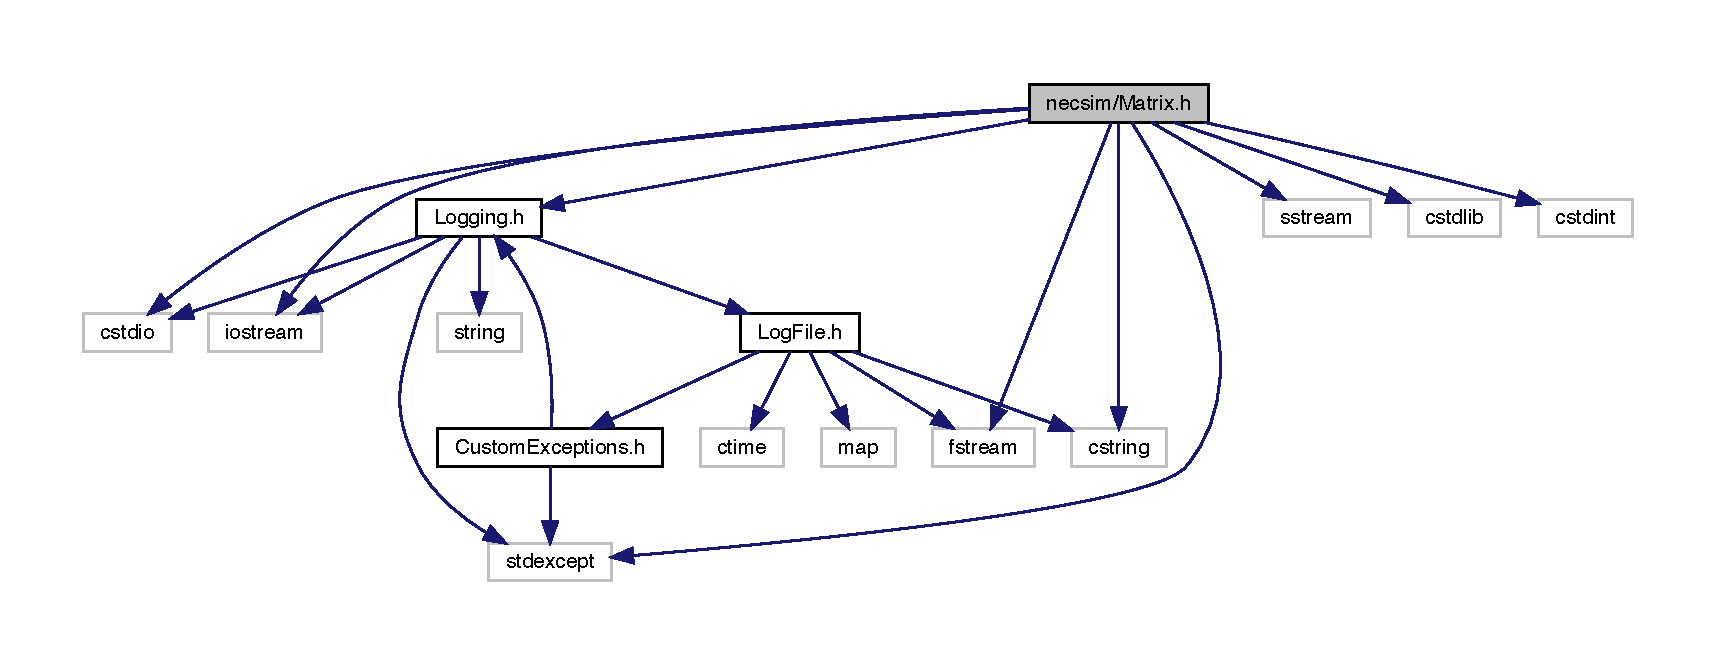
\includegraphics[width=350pt]{_matrix_8h__incl}
\end{center}
\end{figure}
This graph shows which files directly or indirectly include this file\+:\nopagebreak
\begin{figure}[H]
\begin{center}
\leavevmode
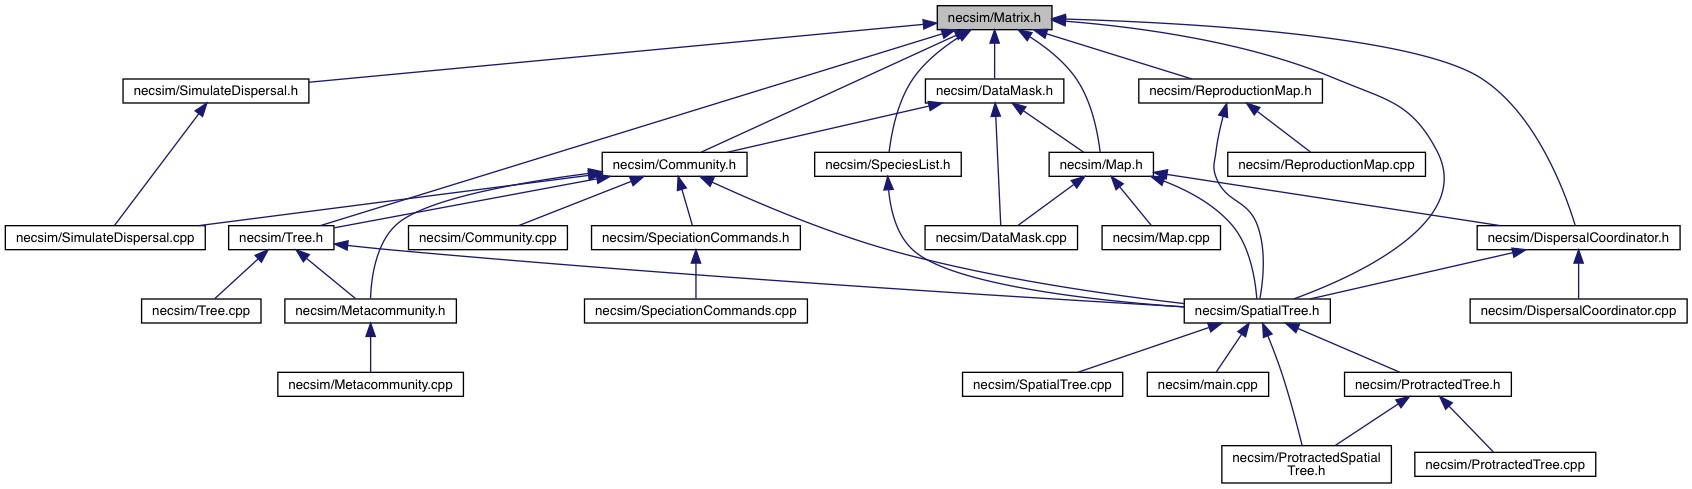
\includegraphics[width=350pt]{_matrix_8h__dep__incl}
\end{center}
\end{figure}
\subsection*{Classes}
\begin{DoxyCompactItemize}
\item 
class \hyperlink{class_row}{Row$<$ T $>$}
\begin{DoxyCompactList}\small\item\em Contains a template \hyperlink{class_row}{Row} class and basic operations. Uses an array to store the row. \end{DoxyCompactList}\item 
class \hyperlink{class_matrix}{Matrix$<$ T $>$}
\begin{DoxyCompactList}\small\item\em A class containing the \hyperlink{class_matrix}{Matrix} object, set up as an array of \hyperlink{class_row}{Row} objects. Includes basic operations, as well as the \hyperlink{class_matrix_aab2f77cfbdbeffcfe67d63d876581b2e}{import\+Csv()} function for more advanced reading from file. \end{DoxyCompactList}\end{DoxyCompactItemize}
\subsection*{Macros}
\begin{DoxyCompactItemize}
\item 
\#define {\bfseries null}~0\hypertarget{_matrix_8h_ac97b8ee753e4405397a42ad5799b0f9e}{}\label{_matrix_8h_ac97b8ee753e4405397a42ad5799b0f9e}

\end{DoxyCompactItemize}
\subsection*{Variables}
\begin{DoxyCompactItemize}
\item 
const int {\bfseries gdal\+\_\+data\+\_\+sizes} \mbox{[}$\,$\mbox{]} = \{0, 8, 16, 16, 32, 32, 32, 64\}\hypertarget{_matrix_8h_a02aa962cfe49d9cc0a492fd0aaf74bd9}{}\label{_matrix_8h_a02aa962cfe49d9cc0a492fd0aaf74bd9}

\end{DoxyCompactItemize}


\subsection{Detailed Description}
Contains a template for a matrix with all the basic matrix operations overloaded. 

\begin{DoxyAuthor}{Author}
Samuel Thompson
\end{DoxyAuthor}
\begin{DoxyCopyright}{Copyright}
\href{https://opensource.org/licenses/BSD-3-Clause}{\tt B\+S\+D-\/3 Licence.}
\end{DoxyCopyright}
Code supplied by James Rosindell with large usage of  href = \char`\"{}http\+://www.\+devarticles.\+com/c/a/\+Cplusplus/\+Operator-\/\+Overloading-\/in-\/\+C-\/plus/1\char`\"{}$>$ this website , and modified and updated by Samuel Thompson. There are two distinct classes, \hyperlink{class_row}{Row} and \hyperlink{class_matrix}{Matrix}. Most operations are low-\/level, but some higher level functions remain, such as import\+Csv().

Contact\+: \href{mailto:thompsonsed@gmail.com}{\tt thompsonsed@gmail.\+com} 
\hypertarget{necsimmodule_8cpp}{}\section{necsimmodule.\+cpp File Reference}
\label{necsimmodule_8cpp}\index{necsimmodule.\+cpp@{necsimmodule.\+cpp}}


Contains the functions allowing integration of the Py\+Coalescence python module directly to the c++.  


{\ttfamily \#include $<$Python.\+h$>$}\\*
{\ttfamily \#include $<$vector$>$}\\*
{\ttfamily \#include $<$string$>$}\\*
{\ttfamily \#include $<$unistd.\+h$>$}\\*
{\ttfamily \#include $<$signal.\+h$>$}\\*
{\ttfamily \#include \char`\"{}Setup.\+h\char`\"{}}\\*
{\ttfamily \#include \char`\"{}Logging.\+h\char`\"{}}\\*
{\ttfamily \#include \char`\"{}CoalescenceTree.\+h\char`\"{}}\\*
{\ttfamily \#include \char`\"{}Protracted\+CoalescenceTree.\+h\char`\"{}}\\*
{\ttfamily \#include \char`\"{}necsimmodule.\+h\char`\"{}}\\*
Include dependency graph for necsimmodule.\+cpp\+:
% FIG 0
\subsection*{Macros}
\begin{DoxyCompactItemize}
\item 
\#define {\bfseries P\+Y\+T\+H\+O\+N\+\_\+\+C\+O\+M\+P\+I\+LE}\hypertarget{necsimmodule_8cpp_a9302692bd9a9cf56478cbae301f04d53}{}\label{necsimmodule_8cpp_a9302692bd9a9cf56478cbae301f04d53}

\item 
\#define {\bfseries I\+N\+I\+T\+E\+R\+R\+OR}~return\hypertarget{necsimmodule_8cpp_a3d94077229c2876134769daeeb28fa8a}{}\label{necsimmodule_8cpp_a3d94077229c2876134769daeeb28fa8a}

\end{DoxyCompactItemize}
\subsection*{Functions}
\begin{DoxyCompactItemize}
\item 
Py\+M\+O\+D\+I\+N\+I\+T\+\_\+\+F\+U\+NC {\bfseries initnecsimmodule} (void)\hypertarget{necsimmodule_8cpp_af5f34a40faeb40208ed217296d73dc1e}{}\label{necsimmodule_8cpp_af5f34a40faeb40208ed217296d73dc1e}

\end{DoxyCompactItemize}
\subsection*{Variables}
\begin{DoxyCompactItemize}
\item 
Py\+Object $\ast$ {\bfseries loggingmodule}\hypertarget{necsimmodule_8cpp_ae269920327ad06583db48e0bb122605e}{}\label{necsimmodule_8cpp_ae269920327ad06583db48e0bb122605e}

\item 
Py\+G\+I\+L\+State\+\_\+\+S\+T\+A\+TE {\bfseries gstate}\hypertarget{necsimmodule_8cpp_ae2ea2c066f7e65f192b08f50adb4ad1d}{}\label{necsimmodule_8cpp_ae2ea2c066f7e65f192b08f50adb4ad1d}

\item 
bool {\bfseries log\+\_\+set} = false\hypertarget{necsimmodule_8cpp_a304b2017ec52852821aced29cb2fe2ed}{}\label{necsimmodule_8cpp_a304b2017ec52852821aced29cb2fe2ed}

\item 
bool {\bfseries logger\+\_\+set} = false\hypertarget{necsimmodule_8cpp_a08d9fbb3de64e2e37d485a6fb7c413c9}{}\label{necsimmodule_8cpp_a08d9fbb3de64e2e37d485a6fb7c413c9}

\item 
Py\+Object $\ast$ {\bfseries logger}\hypertarget{necsimmodule_8cpp_ac5c8cc1b55a6d2753d51817bd568aada}{}\label{necsimmodule_8cpp_ac5c8cc1b55a6d2753d51817bd568aada}

\end{DoxyCompactItemize}


\subsection{Detailed Description}
Contains the functions allowing integration of the Py\+Coalescence python module directly to the c++. 

\begin{DoxyAuthor}{Author}
Samuel Thompson
\end{DoxyAuthor}
\begin{DoxyCopyright}{Copyright}
\href{https://opensource.org/licenses/BSD-3-Clause}{\tt B\+S\+D-\/3 Licence.} 
\end{DoxyCopyright}

\hypertarget{necsimmodule_8h}{}\section{necsimmodule.\+h File Reference}
\label{necsimmodule_8h}\index{necsimmodule.\+h@{necsimmodule.\+h}}


Contains the functions allowing integration of the Py\+Coalescence python module directly to the c++.  


{\ttfamily \#include $<$Python.\+h$>$}\\*
{\ttfamily \#include $<$vector$>$}\\*
{\ttfamily \#include $<$string$>$}\\*
Include dependency graph for necsimmodule.\+h\+:\nopagebreak
\begin{figure}[H]
\begin{center}
\leavevmode
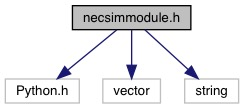
\includegraphics[width=255pt]{necsimmodule_8h__incl}
\end{center}
\end{figure}
This graph shows which files directly or indirectly include this file\+:\nopagebreak
\begin{figure}[H]
\begin{center}
\leavevmode
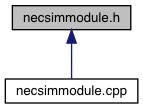
\includegraphics[width=179pt]{necsimmodule_8h__dep__incl}
\end{center}
\end{figure}
\subsection*{Classes}
\begin{DoxyCompactItemize}
\item 
struct \hyperlink{structmodule__state}{module\+\_\+state}
\end{DoxyCompactItemize}
\subsection*{Macros}
\begin{DoxyCompactItemize}
\item 
\#define {\bfseries G\+E\+T\+S\+T\+A\+TE}(m)~(\&\+\_\+state)\hypertarget{necsimmodule_8h_a6d1f389576656b98c42c69f7cf1d55c0}{}\label{necsimmodule_8h_a6d1f389576656b98c42c69f7cf1d55c0}

\item 
\#define {\bfseries I\+N\+I\+T\+E\+R\+R\+OR}~return\hypertarget{necsimmodule_8h_a3d94077229c2876134769daeeb28fa8a}{}\label{necsimmodule_8h_a3d94077229c2876134769daeeb28fa8a}

\end{DoxyCompactItemize}
\subsection*{Functions}
\begin{DoxyCompactItemize}
\item 
Py\+M\+O\+D\+I\+N\+I\+T\+\_\+\+F\+U\+NC {\bfseries initnecsimmodule} (void)\hypertarget{necsimmodule_8h_af5f34a40faeb40208ed217296d73dc1e}{}\label{necsimmodule_8h_af5f34a40faeb40208ed217296d73dc1e}

\end{DoxyCompactItemize}


\subsection{Detailed Description}
Contains the functions allowing integration of the Py\+Coalescence python module directly to the c++. 

\begin{DoxyAuthor}{Author}
Samuel Thompson
\end{DoxyAuthor}
\begin{DoxyCopyright}{Copyright}
\href{https://opensource.org/licenses/BSD-3-Clause}{\tt B\+S\+D-\/3 Licence.} 
\end{DoxyCopyright}

\hypertarget{_protracted_tree_8cpp}{}\section{necsim/\+Protracted\+Tree.cpp File Reference}
\label{_protracted_tree_8cpp}\index{necsim/\+Protracted\+Tree.\+cpp@{necsim/\+Protracted\+Tree.\+cpp}}


Contains the \hyperlink{class_protracted_tree}{Protracted\+Tree} class for running simulations and outputting the phylogenetic trees using protracted speciation.  


{\ttfamily \#include \char`\"{}Protracted\+Tree.\+h\char`\"{}}\\*
Include dependency graph for Protracted\+Tree.\+cpp\+:\nopagebreak
\begin{figure}[H]
\begin{center}
\leavevmode
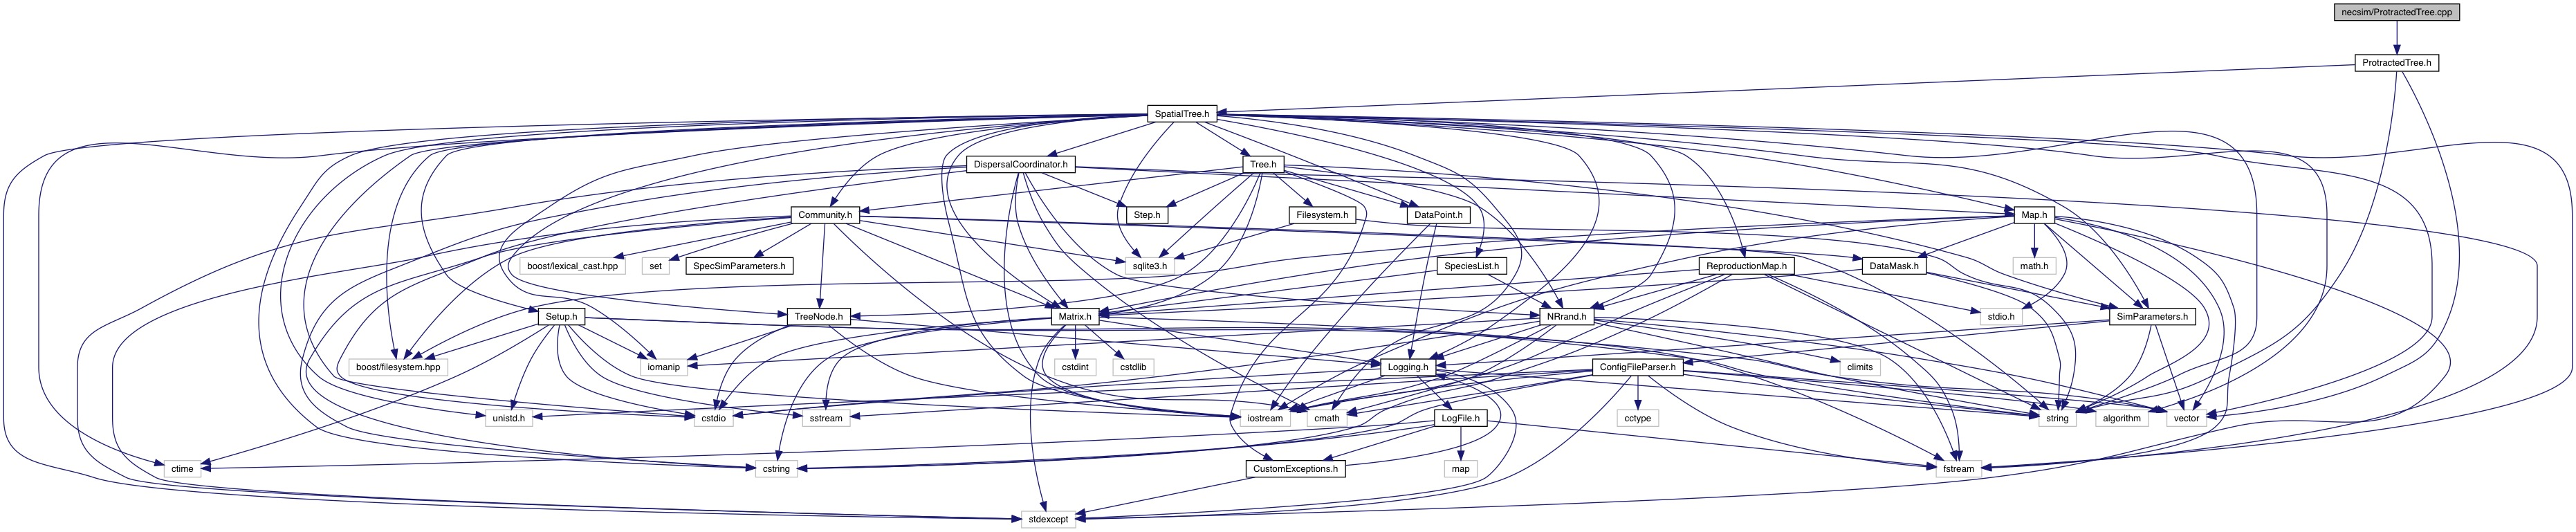
\includegraphics[width=350pt]{_protracted_tree_8cpp__incl}
\end{center}
\end{figure}


\subsection{Detailed Description}
Contains the \hyperlink{class_protracted_tree}{Protracted\+Tree} class for running simulations and outputting the phylogenetic trees using protracted speciation. 

\begin{DoxyAuthor}{Author}
Sam Thompson 
\end{DoxyAuthor}
\begin{DoxyDate}{Date}
12/07/2017
\end{DoxyDate}
Contact\+: \href{mailto:samuel.thompson14@imperial.ac.uk}{\tt samuel.\+thompson14@imperial.\+ac.\+uk} or \href{mailto:thompsonsed@gmail.com}{\tt thompsonsed@gmail.\+com} \begin{DoxyCopyright}{Copyright}
\href{https://opensource.org/licenses/BSD-3-Clause}{\tt B\+S\+D-\/3 Licence.} 
\end{DoxyCopyright}

\hypertarget{_protracted_tree_8h}{}\section{Protracted\+CoalescenceTree.\+h File Reference}
\label{_protracted_tree_8h}\index{Protracted\+CoalescenceTree.\+h@{Protracted\+CoalescenceTree.\+h}}


Contains the \hyperlink{class_protracted_tree}{Protracted\+CoalescenceTree} class for running simulations and outputting the phylogenetic trees using protracted speciation.


{\ttfamily \#include $<$vector$>$}\\*
{\ttfamily \#include $<$string$>$}\\*
{\ttfamily \#include \char`\"{}CoalescenceTree.\+h\char`\"{}}\\*
Include dependency graph for Protracted\+CoalescenceTree.\+h\+:
% FIG 0
This graph shows which files directly or indirectly include this file\+:
% FIG 1
\subsection*{Classes}
\begin{DoxyCompactItemize}
\item 
class \hyperlink{class_protracted_tree}{Protracted\+CoalescenceTree}
\end{DoxyCompactItemize}
\subsection*{Functions}
\begin{DoxyCompactItemize}
\item 
int \hyperlink{_protracted_tree_8h_a694b43a1b415f99e0b6dc5ba43cc156d}{run\+Main\+Protracted} (int argc, vector$<$ string $>$ argv)
\begin{DoxyCompactList}\small\item\em Runs the main simulation using protracted speciation, including all parsing of command line arguments. \end{DoxyCompactList}\end{DoxyCompactItemize}


\subsection{Detailed Description}
Contains the \hyperlink{class_protracted_tree}{Protracted\+CoalescenceTree} class for running simulations and outputting the phylogenetic trees using protracted speciation.

Contains the protracted tree class, for running simulations with procated speciation.

\begin{DoxyAuthor}{Author}
Sam Thompson 
\end{DoxyAuthor}
\begin{DoxyDate}{Date}
12/07/2017
\end{DoxyDate}
Contact\+: \href{mailto:samuel.thompson14@imperial.ac.uk}{\tt samuel.\+thompson14@imperial.\+ac.\+uk} or \href{mailto:thompsonsed@gmail.com}{\tt thompsonsed@gmail.\+com} \begin{DoxyCopyright}{Copyright}
\href{https://opensource.org/licenses/BSD-3-Clause}{\tt B\+S\+D-\/3 Licence.} 
\end{DoxyCopyright}
\begin{DoxyVersion}{Version}
1.\+1
\end{DoxyVersion}


\subsection{Function Documentation}
\index{Protracted\+CoalescenceTree.\+h@{Protracted\+CoalescenceTree.\+h}!run\+Main\+Protracted@{run\+Main\+Protracted}}
\index{run\+Main\+Protracted@{run\+Main\+Protracted}!Protracted\+CoalescenceTree.\+h@{Protracted\+CoalescenceTree.\+h}}
\subsubsection[{\texorpdfstring{run\+Main\+Protracted(int argc, vector$<$ string $>$ argv)}{runMainProtracted(int argc, vector< string > argv)}}]{\setlength{\rightskip}{0pt plus 5cm}int run\+Main\+Protracted (
\begin{DoxyParamCaption}
\item[{int}]{argc, }
\item[{vector$<$ string $>$}]{argv}
\end{DoxyParamCaption}
)}\hypertarget{_protracted_tree_8h_a694b43a1b415f99e0b6dc5ba43cc156d}{}\label{_protracted_tree_8h_a694b43a1b415f99e0b6dc5ba43cc156d}


Runs the main simulation using protracted speciation, including all parsing of command line arguments. 


\begin{DoxyParams}{Parameters}
{\em argv} & \\
\hline
\end{DoxyParams}
\begin{DoxyReturn}{Returns}

\end{DoxyReturn}

\begin{DoxyParams}{Parameters}
{\em argc} & the number of arguments (size of argv) \\
\hline
{\em argv} & the arguments \\
\hline
\end{DoxyParams}
\begin{DoxyReturn}{Returns}
int 0 if successful 
\end{DoxyReturn}

\hypertarget{_reproduction_map_8cpp}{}\section{necsim/\+Reproduction\+Map.cpp File Reference}
\label{_reproduction_map_8cpp}\index{necsim/\+Reproduction\+Map.\+cpp@{necsim/\+Reproduction\+Map.\+cpp}}


Contains the \hyperlink{class_reproduction_map}{Reproduction\+Map}, which inherits from \hyperlink{class_matrix}{Matrix} and adds a few extra parameters.  


{\ttfamily \#include \char`\"{}Reproduction\+Map.\+h\char`\"{}}\\*
Include dependency graph for Reproduction\+Map.\+cpp\+:\nopagebreak
\begin{figure}[H]
\begin{center}
\leavevmode
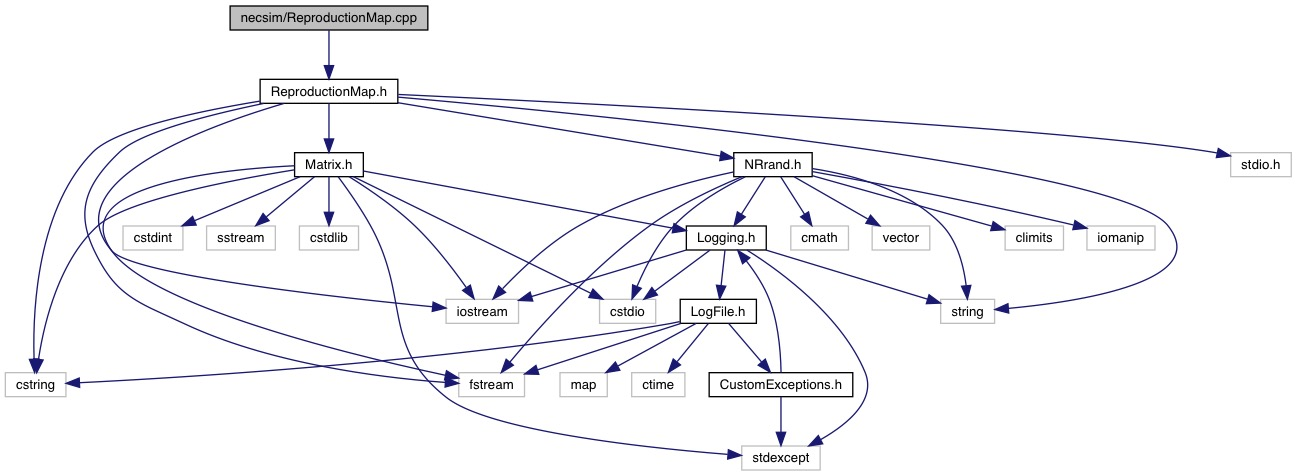
\includegraphics[width=350pt]{_reproduction_map_8cpp__incl}
\end{center}
\end{figure}


\subsection{Detailed Description}
Contains the \hyperlink{class_reproduction_map}{Reproduction\+Map}, which inherits from \hyperlink{class_matrix}{Matrix} and adds a few extra parameters. 

\begin{DoxyAuthor}{Author}
Samuel Thompson 
\end{DoxyAuthor}
\begin{DoxyDate}{Date}
16/08/2017
\end{DoxyDate}
\begin{DoxyCopyright}{Copyright}
\href{https://opensource.org/licenses/BSD-3-Clause}{\tt B\+S\+D-\/3 Licence.} 
\end{DoxyCopyright}

\hypertarget{_reproduction_map_8h}{}\section{necsim/\+Reproduction\+Map.h File Reference}
\label{_reproduction_map_8h}\index{necsim/\+Reproduction\+Map.\+h@{necsim/\+Reproduction\+Map.\+h}}


Contains the \hyperlink{class_reproduction_map}{Reproduction\+Map}, which inherits from \hyperlink{class_matrix}{Matrix} and adds a few extra parameters.  


{\ttfamily \#include $<$cstring$>$}\\*
{\ttfamily \#include $<$string$>$}\\*
{\ttfamily \#include $<$stdio.\+h$>$}\\*
{\ttfamily \#include $<$iostream$>$}\\*
{\ttfamily \#include $<$fstream$>$}\\*
{\ttfamily \#include \char`\"{}Matrix.\+h\char`\"{}}\\*
{\ttfamily \#include \char`\"{}N\+Rrand.\+h\char`\"{}}\\*
Include dependency graph for Reproduction\+Map.\+h\+:\nopagebreak
\begin{figure}[H]
\begin{center}
\leavevmode
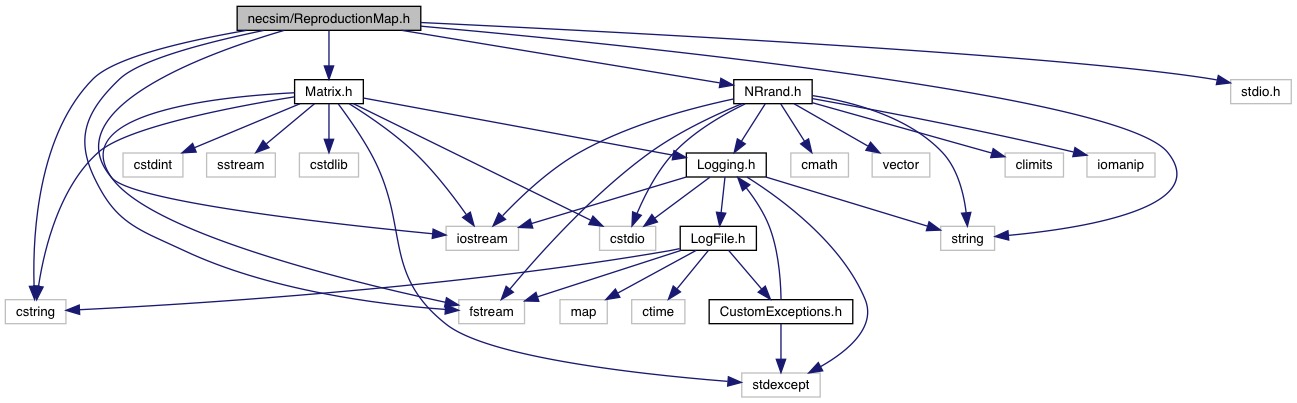
\includegraphics[width=350pt]{_reproduction_map_8h__incl}
\end{center}
\end{figure}
This graph shows which files directly or indirectly include this file\+:\nopagebreak
\begin{figure}[H]
\begin{center}
\leavevmode
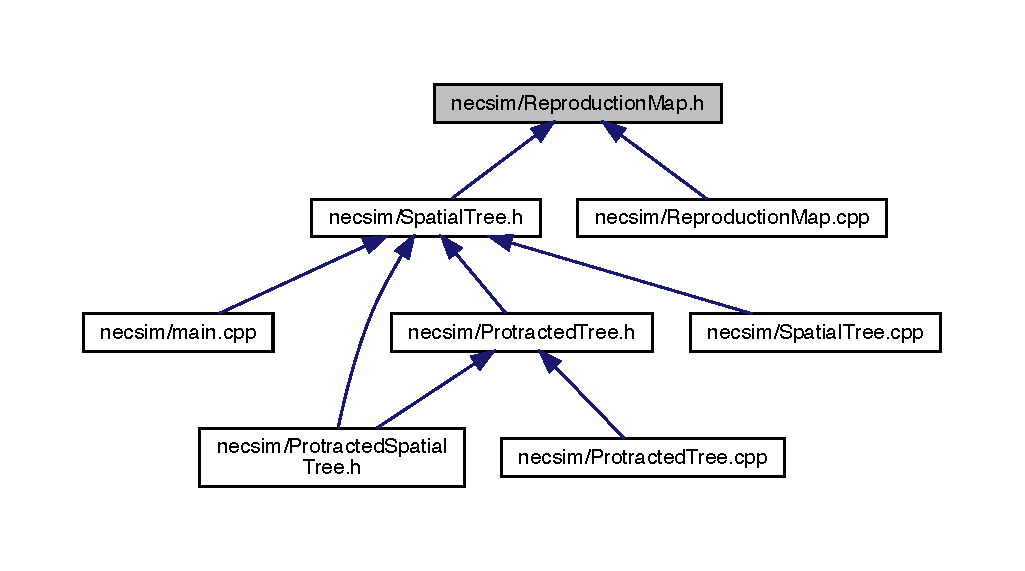
\includegraphics[width=350pt]{_reproduction_map_8h__dep__incl}
\end{center}
\end{figure}
\subsection*{Classes}
\begin{DoxyCompactItemize}
\item 
class \hyperlink{class_reproduction_map}{Reproduction\+Map}
\begin{DoxyCompactList}\small\item\em Contains the routines for importing the reproduction map and getting a cell value from the map. \end{DoxyCompactList}\end{DoxyCompactItemize}


\subsection{Detailed Description}
Contains the \hyperlink{class_reproduction_map}{Reproduction\+Map}, which inherits from \hyperlink{class_matrix}{Matrix} and adds a few extra parameters. 

\begin{DoxyAuthor}{Author}
Samuel Thompson 
\end{DoxyAuthor}
\begin{DoxyDate}{Date}
16/08/2017
\end{DoxyDate}
\begin{DoxyCopyright}{Copyright}
\href{https://opensource.org/licenses/BSD-3-Clause}{\tt B\+S\+D-\/3 Licence.} 
\end{DoxyCopyright}

\hypertarget{_setup_8cpp}{}\section{necsim/\+Setup.cpp File Reference}
\label{_setup_8cpp}\index{necsim/\+Setup.\+cpp@{necsim/\+Setup.\+cpp}}


Contains the command line parsing and setup options for N\+E\+C\+Sim.  


{\ttfamily \#include \char`\"{}Setup.\+h\char`\"{}}\\*
{\ttfamily \#include \char`\"{}Logging.\+h\char`\"{}}\\*
Include dependency graph for Setup.\+cpp\+:\nopagebreak
\begin{figure}[H]
\begin{center}
\leavevmode
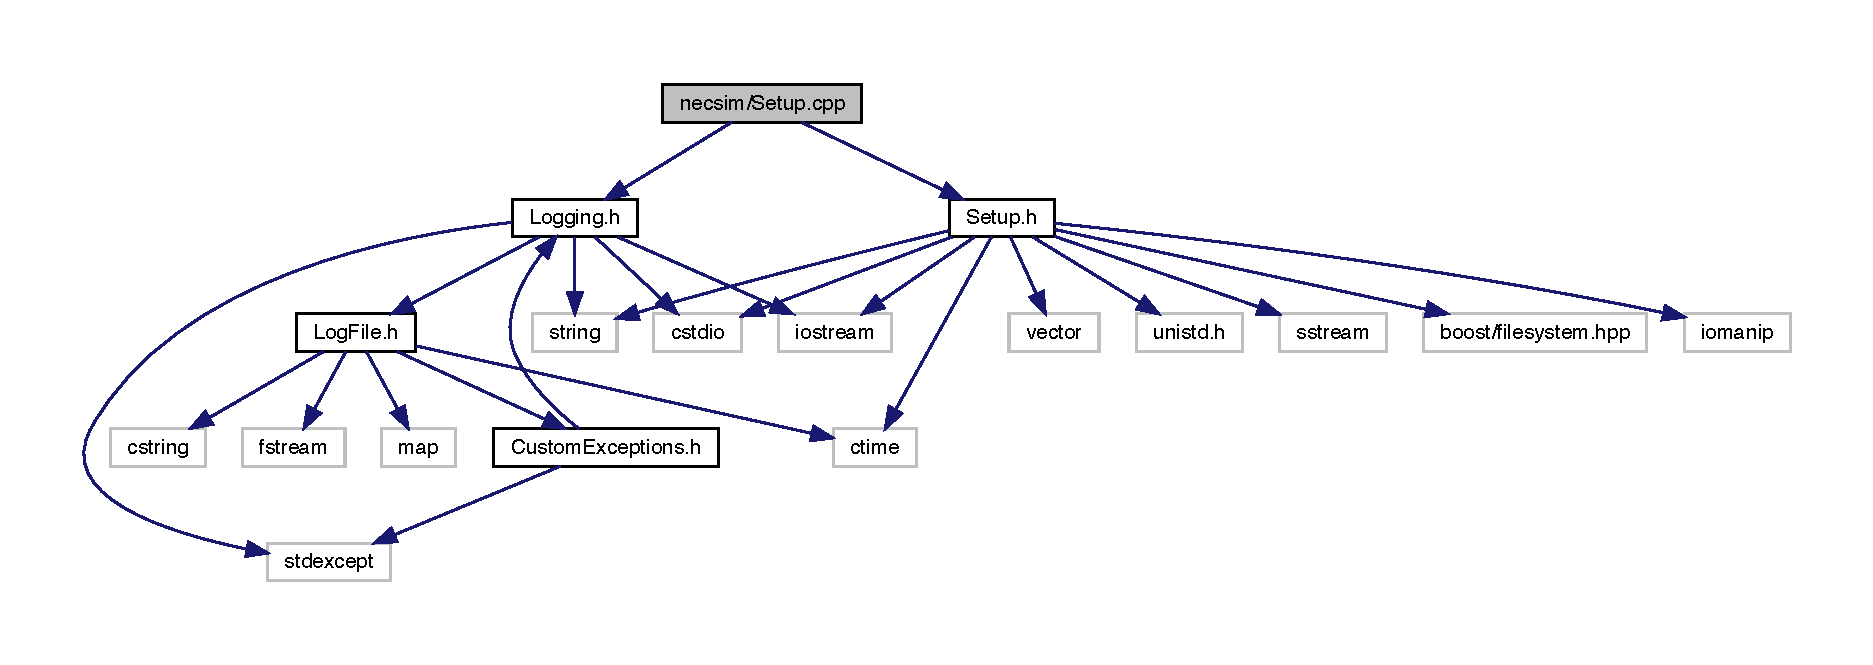
\includegraphics[width=350pt]{_setup_8cpp__incl}
\end{center}
\end{figure}
\subsection*{Functions}
\begin{DoxyCompactItemize}
\item 
void {\bfseries open\+Log\+File} (bool append)\hypertarget{_setup_8cpp_a25e6e7ae1e07841be7b7872521e8ad8b}{}\label{_setup_8cpp_a25e6e7ae1e07841be7b7872521e8ad8b}

\item 
void \hyperlink{_setup_8cpp_ae5f0fe9d930f0bf31869e95f1d284e73}{run\+As\+Default} (vector$<$ string $>$ \&comargs)
\begin{DoxyCompactList}\small\item\em Sets up the command-\/line arguments for default parameters. \end{DoxyCompactList}\item 
void \hyperlink{_setup_8cpp_ae630bc537fa43724bcb8e13905640d4f}{run\+Large} (vector$<$ string $>$ \&comargs)
\begin{DoxyCompactList}\small\item\em Sets up the command-\/line arguments for larger-\/scale default parameters. \end{DoxyCompactList}\item 
void \hyperlink{_setup_8cpp_ac712ff5a067a5d07f3b4c3dc6e5bfad1}{run\+XL} (vector$<$ string $>$ \&comargs)
\begin{DoxyCompactList}\small\item\em Sets up the command-\/line arguments for default very large scale parameters. \end{DoxyCompactList}\item 
void \hyperlink{_setup_8cpp_a297d1a4ce3dd8aa2c7c06c578bd5d80a}{remove\+Com\+Option} (unsigned long \&argc, vector$<$ string $>$ \&comargs)\hypertarget{_setup_8cpp_a297d1a4ce3dd8aa2c7c06c578bd5d80a}{}\label{_setup_8cpp_a297d1a4ce3dd8aa2c7c06c578bd5d80a}

\begin{DoxyCompactList}\small\item\em Removes the command line options supplied, leaving just a clean vector with the correct data in. \end{DoxyCompactList}\end{DoxyCompactItemize}
\subsection*{Variables}
\begin{DoxyCompactItemize}
\item 
string {\bfseries log\+\_\+name} = \char`\"{}null\char`\"{}\hypertarget{_setup_8cpp_a2b3e7c0f4a5a17a01a5157ab01e59a60}{}\label{_setup_8cpp_a2b3e7c0f4a5a17a01a5157ab01e59a60}

\item 
int {\bfseries saved\+\_\+stdout}\hypertarget{_setup_8cpp_abc860612bcc3ce0f446f60f8314195d0}{}\label{_setup_8cpp_abc860612bcc3ce0f446f60f8314195d0}

\end{DoxyCompactItemize}


\subsection{Detailed Description}
Contains the command line parsing and setup options for N\+E\+C\+Sim. 

\begin{DoxyAuthor}{Author}
Sam Thompson
\end{DoxyAuthor}
Contact\+: \href{mailto:samuel.thompson14@imperial.ac.uk}{\tt samuel.\+thompson14@imperial.\+ac.\+uk} or \href{mailto:thompsonsed@gmail.com}{\tt thompsonsed@gmail.\+com} \begin{DoxyCopyright}{Copyright}
\href{https://opensource.org/licenses/BSD-3-Clause}{\tt B\+S\+D-\/3 Licence.} 
\end{DoxyCopyright}


\subsection{Function Documentation}
\index{Setup.\+cpp@{Setup.\+cpp}!run\+As\+Default@{run\+As\+Default}}
\index{run\+As\+Default@{run\+As\+Default}!Setup.\+cpp@{Setup.\+cpp}}
\subsubsection[{\texorpdfstring{run\+As\+Default(vector$<$ string $>$ \&comargs)}{runAsDefault(vector< string > &comargs)}}]{\setlength{\rightskip}{0pt plus 5cm}void run\+As\+Default (
\begin{DoxyParamCaption}
\item[{vector$<$ string $>$ \&}]{comargs}
\end{DoxyParamCaption}
)}\hypertarget{_setup_8cpp_ae5f0fe9d930f0bf31869e95f1d284e73}{}\label{_setup_8cpp_ae5f0fe9d930f0bf31869e95f1d284e73}


Sets up the command-\/line arguments for default parameters. 

This is intended for testing purposes only. 
\begin{DoxyParams}{Parameters}
{\em comargs} & a vector of command-\/line arguments for putting the parameters into. \\
\hline
\end{DoxyParams}
\index{Setup.\+cpp@{Setup.\+cpp}!run\+Large@{run\+Large}}
\index{run\+Large@{run\+Large}!Setup.\+cpp@{Setup.\+cpp}}
\subsubsection[{\texorpdfstring{run\+Large(vector$<$ string $>$ \&comargs)}{runLarge(vector< string > &comargs)}}]{\setlength{\rightskip}{0pt plus 5cm}void run\+Large (
\begin{DoxyParamCaption}
\item[{vector$<$ string $>$ \&}]{comargs}
\end{DoxyParamCaption}
)}\hypertarget{_setup_8cpp_ae630bc537fa43724bcb8e13905640d4f}{}\label{_setup_8cpp_ae630bc537fa43724bcb8e13905640d4f}


Sets up the command-\/line arguments for larger-\/scale default parameters. 

This is intended for testing purposes only. 
\begin{DoxyParams}{Parameters}
{\em comargs} & a vector of command-\/line arguments for putting the parameters into. \\
\hline
\end{DoxyParams}
\index{Setup.\+cpp@{Setup.\+cpp}!run\+XL@{run\+XL}}
\index{run\+XL@{run\+XL}!Setup.\+cpp@{Setup.\+cpp}}
\subsubsection[{\texorpdfstring{run\+X\+L(vector$<$ string $>$ \&comargs)}{runXL(vector< string > &comargs)}}]{\setlength{\rightskip}{0pt plus 5cm}void run\+XL (
\begin{DoxyParamCaption}
\item[{vector$<$ string $>$ \&}]{comargs}
\end{DoxyParamCaption}
)}\hypertarget{_setup_8cpp_ac712ff5a067a5d07f3b4c3dc6e5bfad1}{}\label{_setup_8cpp_ac712ff5a067a5d07f3b4c3dc6e5bfad1}


Sets up the command-\/line arguments for default very large scale parameters. 

This is intended for testing purposes only. 
\begin{DoxyParams}{Parameters}
{\em comargs} & a vector of command-\/line arguments for putting the parameters into. \\
\hline
\end{DoxyParams}

\hypertarget{_setup_8h}{}\section{necsim/\+Setup.h File Reference}
\label{_setup_8h}\index{necsim/\+Setup.\+h@{necsim/\+Setup.\+h}}


Contains declarations for the command line parsing and setup options for N\+E\+C\+Sim.  


{\ttfamily \#include $<$string$>$}\\*
{\ttfamily \#include $<$vector$>$}\\*
{\ttfamily \#include $<$unistd.\+h$>$}\\*
{\ttfamily \#include $<$sstream$>$}\\*
{\ttfamily \#include $<$ctime$>$}\\*
{\ttfamily \#include $<$boost/filesystem.\+hpp$>$}\\*
{\ttfamily \#include $<$cstdio$>$}\\*
{\ttfamily \#include $<$iostream$>$}\\*
{\ttfamily \#include $<$iomanip$>$}\\*
Include dependency graph for Setup.\+h\+:\nopagebreak
\begin{figure}[H]
\begin{center}
\leavevmode
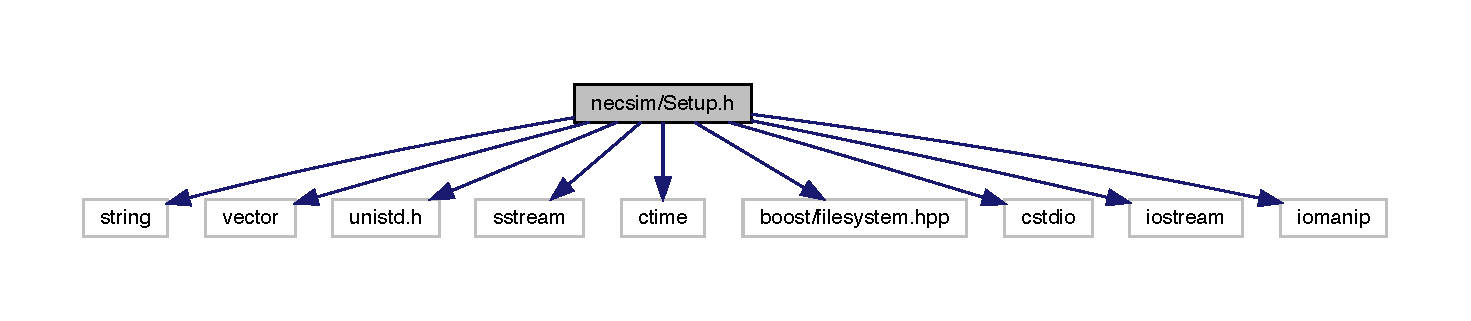
\includegraphics[width=350pt]{_setup_8h__incl}
\end{center}
\end{figure}
This graph shows which files directly or indirectly include this file\+:\nopagebreak
\begin{figure}[H]
\begin{center}
\leavevmode
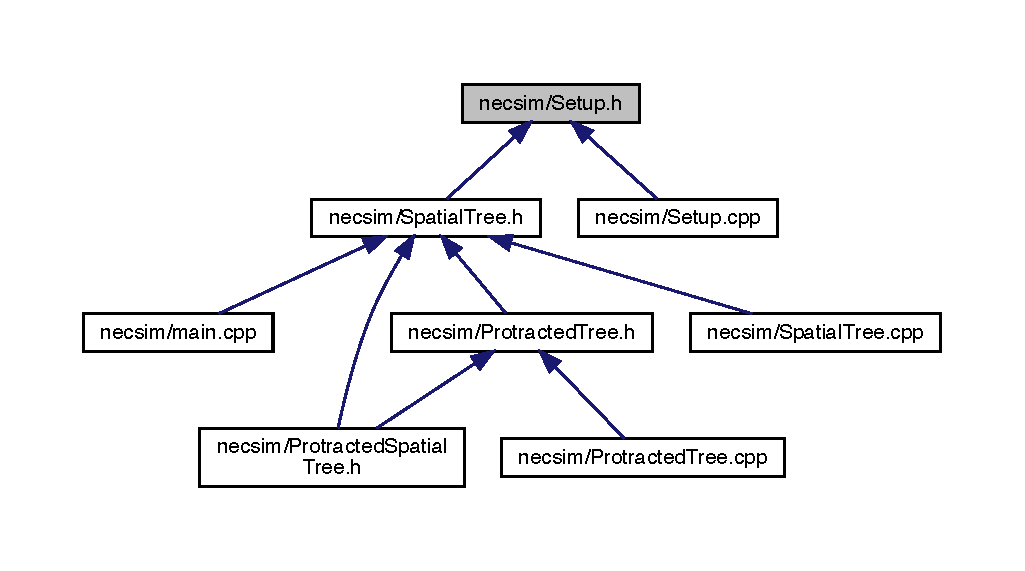
\includegraphics[width=350pt]{_setup_8h__dep__incl}
\end{center}
\end{figure}
\subsection*{Functions}
\begin{DoxyCompactItemize}
\item 
void \hyperlink{_setup_8h_ae5f0fe9d930f0bf31869e95f1d284e73}{run\+As\+Default} (vector$<$ string $>$ \&comargs)
\begin{DoxyCompactList}\small\item\em Sets up the command-\/line arguments for default parameters. \end{DoxyCompactList}\item 
void \hyperlink{_setup_8h_ae630bc537fa43724bcb8e13905640d4f}{run\+Large} (vector$<$ string $>$ \&comargs)
\begin{DoxyCompactList}\small\item\em Sets up the command-\/line arguments for larger-\/scale default parameters. \end{DoxyCompactList}\item 
void \hyperlink{_setup_8h_ac712ff5a067a5d07f3b4c3dc6e5bfad1}{run\+XL} (vector$<$ string $>$ \&comargs)
\begin{DoxyCompactList}\small\item\em Sets up the command-\/line arguments for default very large scale parameters. \end{DoxyCompactList}\item 
void \hyperlink{_setup_8h_a297d1a4ce3dd8aa2c7c06c578bd5d80a}{remove\+Com\+Option} (unsigned long \&argc, vector$<$ string $>$ \&comargs)\hypertarget{_setup_8h_a297d1a4ce3dd8aa2c7c06c578bd5d80a}{}\label{_setup_8h_a297d1a4ce3dd8aa2c7c06c578bd5d80a}

\begin{DoxyCompactList}\small\item\em Removes the command line options supplied, leaving just a clean vector with the correct data in. \end{DoxyCompactList}\end{DoxyCompactItemize}
\subsection*{Variables}
\begin{DoxyCompactItemize}
\item 
string {\bfseries log\+\_\+name}\hypertarget{_setup_8h_a2b3e7c0f4a5a17a01a5157ab01e59a60}{}\label{_setup_8h_a2b3e7c0f4a5a17a01a5157ab01e59a60}

\item 
int {\bfseries saved\+\_\+stdout}\hypertarget{_setup_8h_abc860612bcc3ce0f446f60f8314195d0}{}\label{_setup_8h_abc860612bcc3ce0f446f60f8314195d0}

\end{DoxyCompactItemize}


\subsection{Detailed Description}
Contains declarations for the command line parsing and setup options for N\+E\+C\+Sim. 

\begin{DoxyAuthor}{Author}
Sam Thompson
\end{DoxyAuthor}
Contact\+: \href{mailto:samuel.thompson14@imperial.ac.uk}{\tt samuel.\+thompson14@imperial.\+ac.\+uk} or \href{mailto:thompsonsed@gmail.com}{\tt thompsonsed@gmail.\+com} \begin{DoxyCopyright}{Copyright}
\href{https://opensource.org/licenses/BSD-3-Clause}{\tt B\+S\+D-\/3 Licence.} 
\end{DoxyCopyright}


\subsection{Function Documentation}
\index{Setup.\+h@{Setup.\+h}!run\+As\+Default@{run\+As\+Default}}
\index{run\+As\+Default@{run\+As\+Default}!Setup.\+h@{Setup.\+h}}
\subsubsection[{\texorpdfstring{run\+As\+Default(vector$<$ string $>$ \&comargs)}{runAsDefault(vector< string > &comargs)}}]{\setlength{\rightskip}{0pt plus 5cm}void run\+As\+Default (
\begin{DoxyParamCaption}
\item[{vector$<$ string $>$ \&}]{comargs}
\end{DoxyParamCaption}
)}\hypertarget{_setup_8h_ae5f0fe9d930f0bf31869e95f1d284e73}{}\label{_setup_8h_ae5f0fe9d930f0bf31869e95f1d284e73}


Sets up the command-\/line arguments for default parameters. 

This is intended for testing purposes only. 
\begin{DoxyParams}{Parameters}
{\em comargs} & a vector of command-\/line arguments for putting the parameters into. \\
\hline
\end{DoxyParams}
\index{Setup.\+h@{Setup.\+h}!run\+Large@{run\+Large}}
\index{run\+Large@{run\+Large}!Setup.\+h@{Setup.\+h}}
\subsubsection[{\texorpdfstring{run\+Large(vector$<$ string $>$ \&comargs)}{runLarge(vector< string > &comargs)}}]{\setlength{\rightskip}{0pt plus 5cm}void run\+Large (
\begin{DoxyParamCaption}
\item[{vector$<$ string $>$ \&}]{comargs}
\end{DoxyParamCaption}
)}\hypertarget{_setup_8h_ae630bc537fa43724bcb8e13905640d4f}{}\label{_setup_8h_ae630bc537fa43724bcb8e13905640d4f}


Sets up the command-\/line arguments for larger-\/scale default parameters. 

This is intended for testing purposes only. 
\begin{DoxyParams}{Parameters}
{\em comargs} & a vector of command-\/line arguments for putting the parameters into. \\
\hline
\end{DoxyParams}
\index{Setup.\+h@{Setup.\+h}!run\+XL@{run\+XL}}
\index{run\+XL@{run\+XL}!Setup.\+h@{Setup.\+h}}
\subsubsection[{\texorpdfstring{run\+X\+L(vector$<$ string $>$ \&comargs)}{runXL(vector< string > &comargs)}}]{\setlength{\rightskip}{0pt plus 5cm}void run\+XL (
\begin{DoxyParamCaption}
\item[{vector$<$ string $>$ \&}]{comargs}
\end{DoxyParamCaption}
)}\hypertarget{_setup_8h_ac712ff5a067a5d07f3b4c3dc6e5bfad1}{}\label{_setup_8h_ac712ff5a067a5d07f3b4c3dc6e5bfad1}


Sets up the command-\/line arguments for default very large scale parameters. 

This is intended for testing purposes only. 
\begin{DoxyParams}{Parameters}
{\em comargs} & a vector of command-\/line arguments for putting the parameters into. \\
\hline
\end{DoxyParams}

\hypertarget{_simulate_dispersal_8cpp}{}\section{Simulate\+Dispersal.\+cpp File Reference}
\label{_simulate_dispersal_8cpp}\index{Simulate\+Dispersal.\+cpp@{Simulate\+Dispersal.\+cpp}}


Contains the ability to simulate a given dispersal kernel on a specified density map, outputting the effect dispersal distance distribution to an S\+QL file after n number of dispersal events (specified by the user).  


{\ttfamily \#include \char`\"{}Simulate\+Dispersal.\+h\char`\"{}}\\*
Include dependency graph for Simulate\+Dispersal.\+cpp\+:
% FIG 0


\subsection{Detailed Description}
Contains the ability to simulate a given dispersal kernel on a specified density map, outputting the effect dispersal distance distribution to an S\+QL file after n number of dispersal events (specified by the user). 

\begin{DoxyAuthor}{Author}
Samuel Thompson
\end{DoxyAuthor}
\begin{DoxyCopyright}{Copyright}
\href{https://opensource.org/licenses/BSD-3-Clause}{\tt B\+S\+D-\/3 Licence.} 
\end{DoxyCopyright}

\hypertarget{_simulate_dispersal_8h}{}\section{Simulate\+Dispersal.\+h File Reference}
\label{_simulate_dispersal_8h}\index{Simulate\+Dispersal.\+h@{Simulate\+Dispersal.\+h}}


Contains the ability to simulate a given dispersal kernel on a specified density map, outputting the effect dispersal distance distribution to an S\+QL file after n number of dispersal events (specified by the user).  


{\ttfamily \#include $<$string$>$}\\*
{\ttfamily \#include $<$stdio.\+h$>$}\\*
{\ttfamily \#include $<$vector$>$}\\*
{\ttfamily \#include $<$iostream$>$}\\*
{\ttfamily \#include $<$fstream$>$}\\*
{\ttfamily \#include $<$math.\+h$>$}\\*
{\ttfamily \#include $<$stdexcept$>$}\\*
{\ttfamily \#include $<$sqlite3.\+h$>$}\\*
{\ttfamily \#include \char`\"{}Matrix.\+h\char`\"{}}\\*
{\ttfamily \#include \char`\"{}Custom\+Exceptions.\+h\char`\"{}}\\*
{\ttfamily \#include \char`\"{}Fattaildeviate.\+h\char`\"{}}\\*
Include dependency graph for Simulate\+Dispersal.\+h\+:
% FIG 0
This graph shows which files directly or indirectly include this file\+:
% FIG 1
\subsection*{Classes}
\begin{DoxyCompactItemize}
\item 
class \hyperlink{struct_cell}{Cell}
\begin{DoxyCompactList}\small\item\em Simple structure containing the x and y positions of a cell. \end{DoxyCompactList}\item 
class \hyperlink{class_simulate_dispersal}{Simulate\+Dispersal}
\begin{DoxyCompactList}\small\item\em Contains routines for importing a density map file, running a dispersal kernel n times on a landscape and record the dispersal distances. \end{DoxyCompactList}\end{DoxyCompactItemize}


\subsection{Detailed Description}
Contains the ability to simulate a given dispersal kernel on a specified density map, outputting the effect dispersal distance distribution to an S\+QL file after n number of dispersal events (specified by the user). 

\begin{DoxyAuthor}{Author}
Samuel Thompson
\end{DoxyAuthor}
\begin{DoxyCopyright}{Copyright}
\href{https://opensource.org/licenses/BSD-3-Clause}{\tt B\+S\+D-\/3 Licence.} 
\end{DoxyCopyright}

\hypertarget{_speciation_counter_8cpp}{}\section{Speciation\+Counter.\+cpp File Reference}
\label{_speciation_counter_8cpp}\index{Speciation\+Counter.\+cpp@{Speciation\+Counter.\+cpp}}


Performs calculations of the coalescence tree structure and generates the S\+QL database objects.  


{\ttfamily \#include \char`\"{}necsim/\+Speciation\+Commands.\+h\char`\"{}}\\*
Include dependency graph for Speciation\+Counter.\+cpp\+:\nopagebreak
\begin{figure}[H]
\begin{center}
\leavevmode
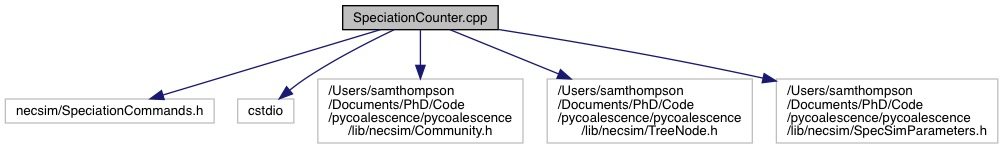
\includegraphics[width=350pt]{_speciation_counter_8cpp__incl}
\end{center}
\end{figure}
\subsection*{Functions}
\begin{DoxyCompactItemize}
\item 
int \hyperlink{_speciation_counter_8cpp_a3c04138a5bfe5d72780bb7e82a18e627}{main} (int argc, char $\ast$$\ast$argv)
\begin{DoxyCompactList}\small\item\em The main Speciation\+Counter routine. \end{DoxyCompactList}\end{DoxyCompactItemize}


\subsection{Detailed Description}
Performs calculations of the coalescence tree structure and generates the S\+QL database objects. 

\begin{DoxyAuthor}{Author}
Samuel Thompson 
\end{DoxyAuthor}
\begin{DoxyDate}{Date}
31/08/16
\end{DoxyDate}
\begin{DoxyCopyright}{Copyright}
\href{https://opensource.org/licenses/BSD-3-Clause}{\tt B\+S\+D-\/3 Licence.} Requires command line parameters and generates a data object from them. Contact\+: \href{mailto:samuel.thompson14@imperial.ac.uk}{\tt samuel.\+thompson14@imperial.\+ac.\+uk} or \href{mailto:thompsonsed@gmail.com}{\tt thompsonsed@gmail.\+com} 
\end{DoxyCopyright}


\subsection{Function Documentation}
\index{Speciation\+Counter.\+cpp@{Speciation\+Counter.\+cpp}!main@{main}}
\index{main@{main}!Speciation\+Counter.\+cpp@{Speciation\+Counter.\+cpp}}
\subsubsection[{\texorpdfstring{main(int argc, char $\ast$$\ast$argv)}{main(int argc, char **argv)}}]{\setlength{\rightskip}{0pt plus 5cm}int main (
\begin{DoxyParamCaption}
\item[{int}]{argc, }
\item[{char $\ast$$\ast$}]{argv}
\end{DoxyParamCaption}
)}\hypertarget{_speciation_counter_8cpp_a3c04138a5bfe5d72780bb7e82a18e627}{}\label{_speciation_counter_8cpp_a3c04138a5bfe5d72780bb7e82a18e627}


The main Speciation\+Counter routine. 


\begin{DoxyParams}{Parameters}
{\em argc} & the number of command line arguments. \\
\hline
{\em argv} & a pointer to an array of the command line arguments. \\
\hline
\end{DoxyParams}
\begin{DoxyReturn}{Returns}
an integer, 0 representing success, anything else representing program failure. 
\end{DoxyReturn}

\hypertarget{_species_list_8h}{}\section{necsim/\+Species\+List.h File Reference}
\label{_species_list_8h}\index{necsim/\+Species\+List.\+h@{necsim/\+Species\+List.\+h}}


Contains the \hyperlink{class_species_list}{Species\+List} class for usage in coalescence simulations.  


{\ttfamily \#include \char`\"{}Matrix.\+h\char`\"{}}\\*
{\ttfamily \#include \char`\"{}N\+Rrand.\+h\char`\"{}}\\*
Include dependency graph for Species\+List.\+h\+:\nopagebreak
\begin{figure}[H]
\begin{center}
\leavevmode
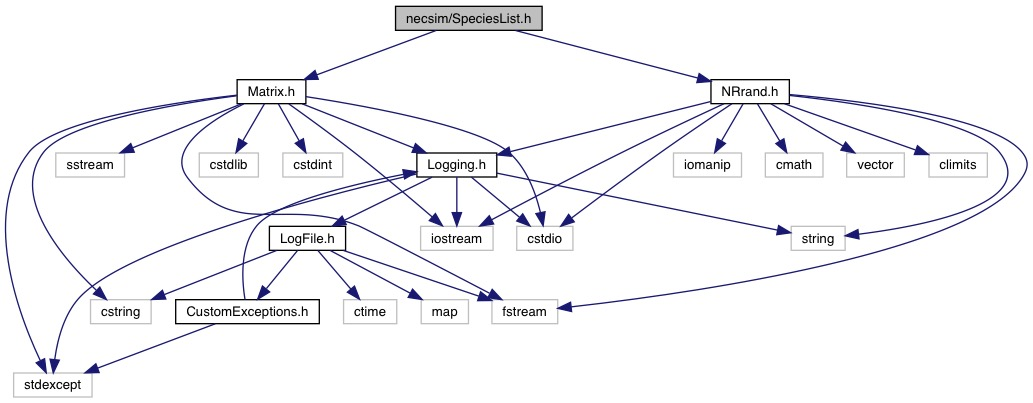
\includegraphics[width=350pt]{_species_list_8h__incl}
\end{center}
\end{figure}
This graph shows which files directly or indirectly include this file\+:\nopagebreak
\begin{figure}[H]
\begin{center}
\leavevmode
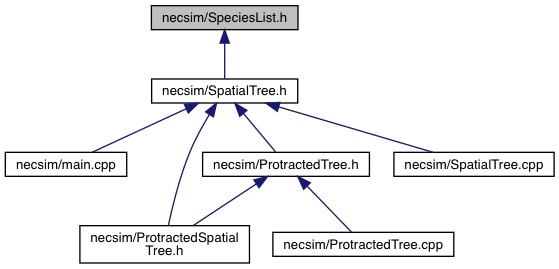
\includegraphics[width=350pt]{_species_list_8h__dep__incl}
\end{center}
\end{figure}
\subsection*{Classes}
\begin{DoxyCompactItemize}
\item 
class \hyperlink{class_species_list}{Species\+List}
\begin{DoxyCompactList}\small\item\em Contains a list of the species that exist at one location. The \hyperlink{class_row}{Row} object, list, contains the active reference number, for looking up the lineage in a \hyperlink{class_row}{Row} of Datapoint objects. Also contains the functions for correctly generating coalescence probabilities and list management. \end{DoxyCompactList}\end{DoxyCompactItemize}


\subsection{Detailed Description}
Contains the \hyperlink{class_species_list}{Species\+List} class for usage in coalescence simulations. 

\begin{DoxyAuthor}{Author}
Samuel Thompson
\end{DoxyAuthor}
\begin{DoxyCopyright}{Copyright}
\href{https://opensource.org/licenses/BSD-3-Clause}{\tt B\+S\+D-\/3 Licence.} 
\end{DoxyCopyright}

\hypertarget{_step_8h}{}\section{necsim/\+Step.h File Reference}
\label{_step_8h}\index{necsim/\+Step.\+h@{necsim/\+Step.\+h}}


Contains the \hyperlink{struct_step}{Step} class for storing required data during a single step of a coalescence simulation.  


This graph shows which files directly or indirectly include this file\+:
\nopagebreak
\begin{figure}[H]
\begin{center}
\leavevmode
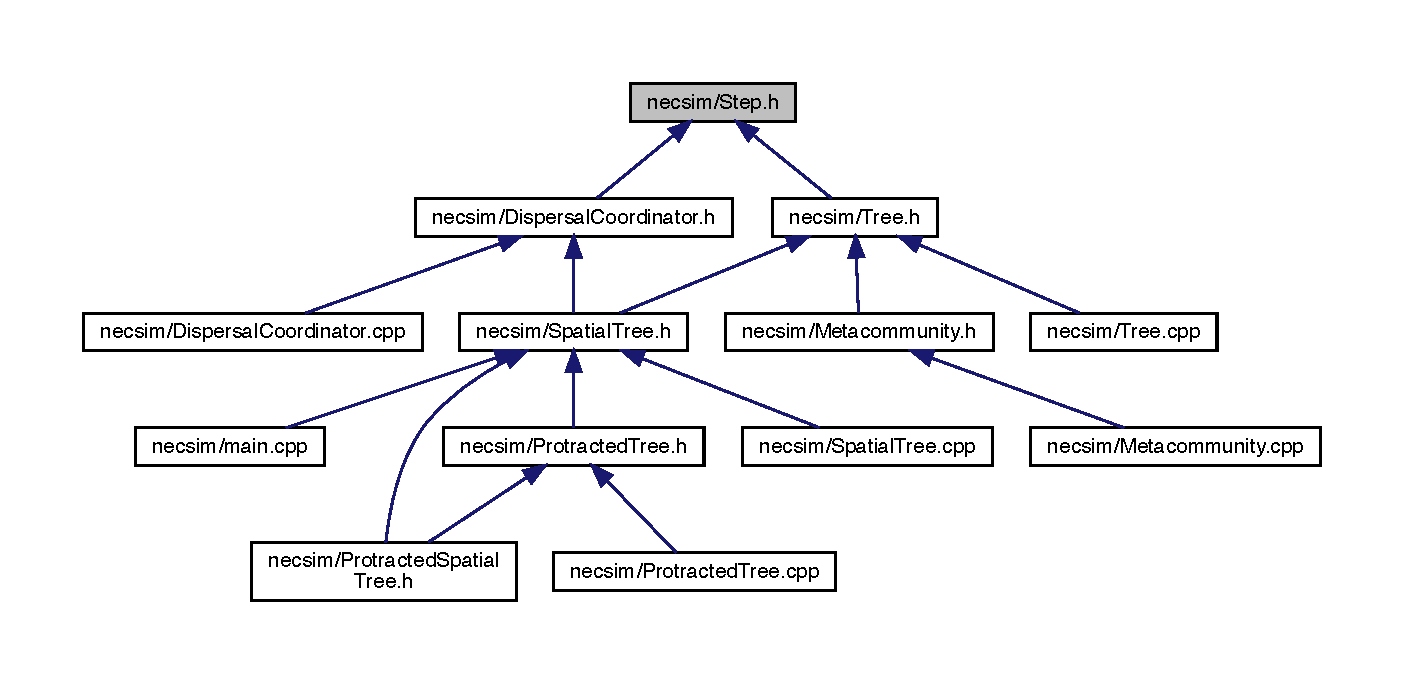
\includegraphics[width=350pt]{_step_8h__dep__incl}
\end{center}
\end{figure}
\subsection*{Classes}
\begin{DoxyCompactItemize}
\item 
class \hyperlink{struct_step}{Step}
\begin{DoxyCompactList}\small\item\em Stores the elements associated with a single step in a coalescence simulation. \end{DoxyCompactList}\end{DoxyCompactItemize}


\subsection{Detailed Description}
Contains the \hyperlink{struct_step}{Step} class for storing required data during a single step of a coalescence simulation. 

\begin{DoxyAuthor}{Author}
Sam Thompson 
\end{DoxyAuthor}
\begin{DoxyDate}{Date}
09/08/2017
\end{DoxyDate}
\begin{DoxyCopyright}{Copyright}
\href{https://opensource.org/licenses/BSD-3-Clause}{\tt B\+S\+D-\/3 Licence.} 
\end{DoxyCopyright}

\hypertarget{_tree_8cpp}{}\section{CoalescenceTree.\+cpp File Reference}
\label{_tree_8cpp}\index{CoalescenceTree.\+cpp@{CoalescenceTree.\+cpp}}


Contains the \hyperlink{class_tree}{CoalescenceTree} class implementation as the main simulation object for spatially-\/explicit coalescence simulations.


{\ttfamily \#include \char`\"{}CoalescenceTree.\+h\char`\"{}}\\*
Include dependency graph for CoalescenceTree.\+cpp\+:
% FIG 0
\subsection*{Functions}
\begin{DoxyCompactItemize}
\item 
int \hyperlink{_tree_8cpp_af60f51c97037bdbe5e9ac92db838ebfd}{run\+Main} (int argc, vector$<$ string $>$ \&argv)
\begin{DoxyCompactList}\small\item\em Runs the main simulation, including all parsing of command line arguments. \end{DoxyCompactList}\end{DoxyCompactItemize}


\subsection{Detailed Description}
Contains the \hyperlink{class_tree}{CoalescenceTree} class implementation as the main simulation object for spatially-\/explicit coalescence simulations.

\begin{DoxyAuthor}{Author}
Samuel Thompson 
\end{DoxyAuthor}
\begin{DoxyDate}{Date}
24/03/17
\end{DoxyDate}
\begin{DoxyVersion}{Version}
1.\+1 
\end{DoxyVersion}
\begin{DoxyCopyright}{Copyright}
\href{https://opensource.org/licenses/BSD-3-Clause}{\tt B\+S\+D-\/3 Licence.} 
\end{DoxyCopyright}


\subsection{Function Documentation}
\index{CoalescenceTree.\+cpp@{CoalescenceTree.\+cpp}!run\+Main@{run\+Main}}
\index{run\+Main@{run\+Main}!CoalescenceTree.\+cpp@{CoalescenceTree.\+cpp}}
\subsubsection[{\texorpdfstring{run\+Main(int argc, vector$<$ string $>$ \&argv)}{runMain(int argc, vector< string > &argv)}}]{\setlength{\rightskip}{0pt plus 5cm}int run\+Main (
\begin{DoxyParamCaption}
\item[{int}]{argc, }
\item[{vector$<$ string $>$ \&}]{argv}
\end{DoxyParamCaption}
)}\hypertarget{_tree_8cpp_af60f51c97037bdbe5e9ac92db838ebfd}{}\label{_tree_8cpp_af60f51c97037bdbe5e9ac92db838ebfd}


Runs the main simulation, including all parsing of command line arguments. 


\begin{DoxyParams}{Parameters}
{\em argc} & the number of arguments (size of argv) \\
\hline
{\em argv} & the arguments \\
\hline
\end{DoxyParams}
\begin{DoxyReturn}{Returns}
int 0 if successful 
\end{DoxyReturn}

\hypertarget{_tree_8h}{}\section{necsim/\+Tree.h File Reference}
\label{_tree_8h}\index{necsim/\+Tree.\+h@{necsim/\+Tree.\+h}}


Contains the \hyperlink{class_tree}{Tree} class implementation as the main simulation object for spatially-\/implicit coalescence simulations. Provides the basis for spatially-\/explicit versions in \hyperlink{class_spatial_tree}{Spatial\+Tree}, and protracted speciation versions in \hyperlink{class_protracted_tree}{Protracted\+Tree} and \hyperlink{class_protracted_spatial_tree}{Protracted\+Spatial\+Tree}.  


{\ttfamily \#include $<$sqlite3.\+h$>$}\\*
{\ttfamily \#include \char`\"{}Tree\+Node.\+h\char`\"{}}\\*
{\ttfamily \#include \char`\"{}Matrix.\+h\char`\"{}}\\*
{\ttfamily \#include \char`\"{}Sim\+Parameters.\+h\char`\"{}}\\*
{\ttfamily \#include \char`\"{}N\+Rrand.\+h\char`\"{}}\\*
{\ttfamily \#include \char`\"{}Data\+Point.\+h\char`\"{}}\\*
{\ttfamily \#include \char`\"{}Community.\+h\char`\"{}}\\*
{\ttfamily \#include \char`\"{}Filesystem.\+h\char`\"{}}\\*
{\ttfamily \#include \char`\"{}Custom\+Exceptions.\+h\char`\"{}}\\*
{\ttfamily \#include \char`\"{}Step.\+h\char`\"{}}\\*
Include dependency graph for Tree.\+h\+:\nopagebreak
\begin{figure}[H]
\begin{center}
\leavevmode
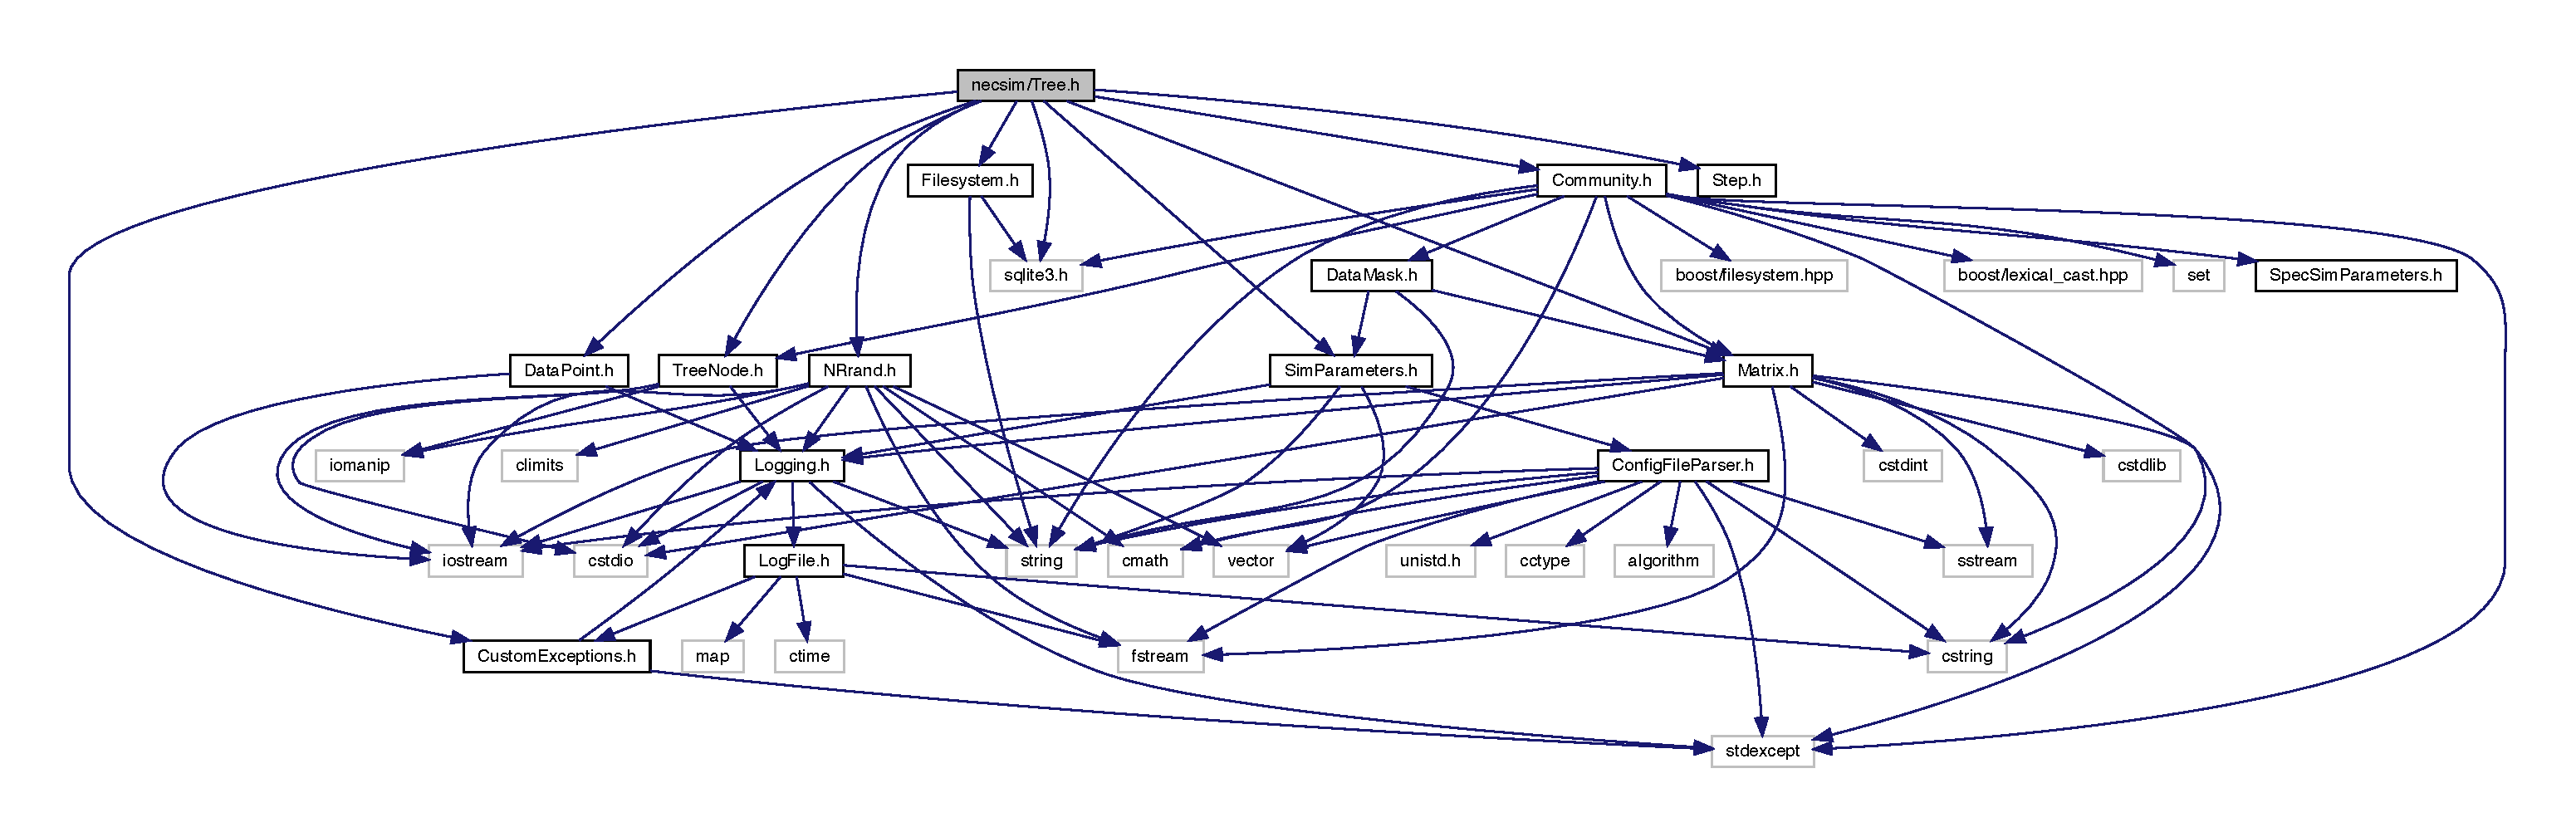
\includegraphics[width=350pt]{_tree_8h__incl}
\end{center}
\end{figure}
This graph shows which files directly or indirectly include this file\+:\nopagebreak
\begin{figure}[H]
\begin{center}
\leavevmode
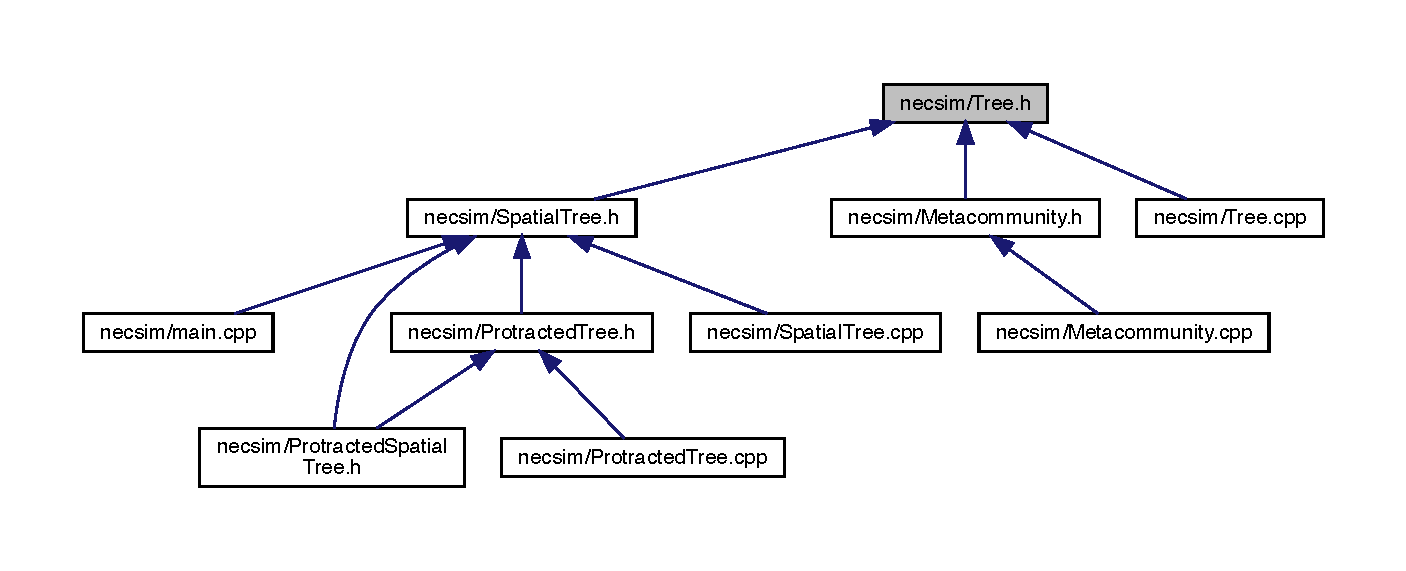
\includegraphics[width=350pt]{_tree_8h__dep__incl}
\end{center}
\end{figure}
\subsection*{Classes}
\begin{DoxyCompactItemize}
\item 
class \hyperlink{class_tree}{Tree}
\end{DoxyCompactItemize}


\subsection{Detailed Description}
Contains the \hyperlink{class_tree}{Tree} class implementation as the main simulation object for spatially-\/implicit coalescence simulations. Provides the basis for spatially-\/explicit versions in \hyperlink{class_spatial_tree}{Spatial\+Tree}, and protracted speciation versions in \hyperlink{class_protracted_tree}{Protracted\+Tree} and \hyperlink{class_protracted_spatial_tree}{Protracted\+Spatial\+Tree}. 

Main simulation class for performing a non-\/spatial neutral simulation and generating the phylogenetic tree of the individuals.

\begin{DoxyAuthor}{Author}
Samuel Thompson 
\end{DoxyAuthor}
\begin{DoxyDate}{Date}
24/03/17
\end{DoxyDate}
\begin{DoxyCopyright}{Copyright}
\href{https://opensource.org/licenses/BSD-3-Clause}{\tt B\+S\+D-\/3 Licence.}
\end{DoxyCopyright}

\hypertarget{_treelist_8cpp}{}\section{Treelist.\+cpp File Reference}
\label{_treelist_8cpp}\index{Treelist.\+cpp@{Treelist.\+cpp}}


Contains the \hyperlink{class_treelist}{Treelist} class implementation, which is used for reconstructing the coalescence tree after simulations are complete. The primary file used by \hyperlink{_treelist_8cpp}{Treelist.\+cpp} and \hyperlink{_speciation_counter_8cpp}{Speciation\+Counter.\+cpp}.  


{\ttfamily \#include \char`\"{}Treelist.\+h\char`\"{}}\\*
Include dependency graph for Treelist.\+cpp\+:
% FIG 0
\subsection*{Functions}
\begin{DoxyCompactItemize}
\item 
bool \hyperlink{_treelist_8cpp_a1c73a46f1e683f85654b643e85a379b8}{check\+Speciation} (const long double \&random\+\_\+number, const long double \&speciation\+\_\+rate, const int \&no\+\_\+generations)
\begin{DoxyCompactList}\small\item\em Checks whether speciation has occured for the provided parameters. Provided here for ease of use when bug-\/fixing. \end{DoxyCompactList}\item 
bool \hyperlink{_treelist_8cpp_a7d6dcddec98b5a2e2310370a2a11b3ab}{double\+Compare} (double d1, double d2, double epsilon)
\begin{DoxyCompactList}\small\item\em Compares two doubles and returns a boolean of whether they are equal, within the epsilon deviation. This is useful for floating point errors in saving and reading doubles from file. \end{DoxyCompactList}\end{DoxyCompactItemize}


\subsection{Detailed Description}
Contains the \hyperlink{class_treelist}{Treelist} class implementation, which is used for reconstructing the coalescence tree after simulations are complete. The primary file used by \hyperlink{_treelist_8cpp}{Treelist.\+cpp} and \hyperlink{_speciation_counter_8cpp}{Speciation\+Counter.\+cpp}. 

\begin{DoxyAuthor}{Author}
Samuel Thompson
\end{DoxyAuthor}
For use with Coal\+\_\+sim 3.\+1 and above. \begin{DoxyCopyright}{Copyright}
\href{https://opensource.org/licenses/BSD-3-Clause}{\tt B\+S\+D-\/3 Licence.} 
\end{DoxyCopyright}


\subsection{Function Documentation}
\index{Treelist.\+cpp@{Treelist.\+cpp}!check\+Speciation@{check\+Speciation}}
\index{check\+Speciation@{check\+Speciation}!Treelist.\+cpp@{Treelist.\+cpp}}
\subsubsection[{\texorpdfstring{check\+Speciation(const long double \&random\+\_\+number, const long double \&speciation\+\_\+rate, const int \&no\+\_\+generations)}{checkSpeciation(const long double &random_number, const long double &speciation_rate, const int &no_generations)}}]{\setlength{\rightskip}{0pt plus 5cm}bool check\+Speciation (
\begin{DoxyParamCaption}
\item[{const long double \&}]{random\+\_\+number, }
\item[{const long double \&}]{speciation\+\_\+rate, }
\item[{const int \&}]{no\+\_\+generations}
\end{DoxyParamCaption}
)}\hypertarget{_treelist_8cpp_a1c73a46f1e683f85654b643e85a379b8}{}\label{_treelist_8cpp_a1c73a46f1e683f85654b643e85a379b8}


Checks whether speciation has occured for the provided parameters. Provided here for ease of use when bug-\/fixing. 


\begin{DoxyParams}{Parameters}
{\em random\+\_\+number} & the random number associated with a lineage \\
\hline
{\em speciation\+\_\+rate} & the global speciation rate \\
\hline
{\em number\+\_\+of\+\_\+generations} & the number of generations the lineage has existed \\
\hline
\end{DoxyParams}
\begin{DoxyReturn}{Returns}
bool the speciation state of the lineage 
\end{DoxyReturn}
\index{Treelist.\+cpp@{Treelist.\+cpp}!double\+Compare@{double\+Compare}}
\index{double\+Compare@{double\+Compare}!Treelist.\+cpp@{Treelist.\+cpp}}
\subsubsection[{\texorpdfstring{double\+Compare(double d1, double d2, double epsilon)}{doubleCompare(double d1, double d2, double epsilon)}}]{\setlength{\rightskip}{0pt plus 5cm}bool double\+Compare (
\begin{DoxyParamCaption}
\item[{double}]{d1, }
\item[{double}]{d2, }
\item[{double}]{epsilon}
\end{DoxyParamCaption}
)}\hypertarget{_treelist_8cpp_a7d6dcddec98b5a2e2310370a2a11b3ab}{}\label{_treelist_8cpp_a7d6dcddec98b5a2e2310370a2a11b3ab}


Compares two doubles and returns a boolean of whether they are equal, within the epsilon deviation. This is useful for floating point errors in saving and reading doubles from file. 


\begin{DoxyParams}{Parameters}
{\em d1} & the first double. \\
\hline
{\em d2} & the second double. \\
\hline
{\em epsilon} & the deviation within which the values are assumed to be equal. \\
\hline
\end{DoxyParams}
\begin{DoxyReturn}{Returns}

\end{DoxyReturn}

\hypertarget{_treelist_8h}{}\section{Treelist.\+h File Reference}
\label{_treelist_8h}\index{Treelist.\+h@{Treelist.\+h}}


Contains the \hyperlink{class_treelist}{Treelist} object, which is used for reconstructing the coalescence tree after simulations are complete. The primary file used by \hyperlink{_treelist_8cpp}{Treelist.\+cpp} and \hyperlink{_speciation_counter_8cpp}{Speciation\+Counter.\+cpp}.  


{\ttfamily \#include $<$math.\+h$>$}\\*
{\ttfamily \#include $<$sqlite3.\+h$>$}\\*
{\ttfamily \#include $<$cstring$>$}\\*
{\ttfamily \#include $<$cmath$>$}\\*
{\ttfamily \#include $<$stdexcept$>$}\\*
{\ttfamily \#include $<$string$>$}\\*
{\ttfamily \#include $<$boost/filesystem.\+hpp$>$}\\*
{\ttfamily \#include $<$boost/lexical\+\_\+cast.\+hpp$>$}\\*
{\ttfamily \#include \char`\"{}Custom\+Exceptions.\+h\char`\"{}}\\*
{\ttfamily \#include \char`\"{}Logging.\+h\char`\"{}}\\*
{\ttfamily \#include \char`\"{}Treenode.\+h\char`\"{}}\\*
{\ttfamily \#include \char`\"{}Matrix.\+h\char`\"{}}\\*
{\ttfamily \#include \char`\"{}Datamask.\+h\char`\"{}}\\*
Include dependency graph for Treelist.\+h\+:
% FIG 0
This graph shows which files directly or indirectly include this file\+:
% FIG 1
\subsection*{Classes}
\begin{DoxyCompactItemize}
\item 
struct \hyperlink{struct_previous_calc_pair}{Previous\+Calc\+Pair}
\begin{DoxyCompactList}\small\item\em A struct for containing pairs of previous calculations to make sure that aren\textquotesingle{}t repeated. \end{DoxyCompactList}\item 
struct \hyperlink{struct_calc_pair_array}{Calc\+Pair\+Array}
\begin{DoxyCompactList}\small\item\em A structure for containing an array of previous calculation information, including which fragments have been already calculated for. \end{DoxyCompactList}\item 
struct \hyperlink{struct_fragment}{Fragment}
\begin{DoxyCompactList}\small\item\em Contains the information needed for defining a fragment. Fragments can be detected from the \hyperlink{class_samplematrix}{Samplematrix} object (which only detects rectangular fragments), or (preferably) is read from an input file. Currently all fragments must be rectangular, although they can be larger than the intended shape if necesssary. \end{DoxyCompactList}\item 
class \hyperlink{class_samplematrix}{Samplematrix}
\begin{DoxyCompactList}\small\item\em A child of the \hyperlink{class_matrix}{Matrix} class as booleans. Used for determining where to sample species from. \end{DoxyCompactList}\item 
class \hyperlink{class_treelist}{Treelist}
\begin{DoxyCompactList}\small\item\em A class to contain the tree object lineages and reconstructing the coalescence tree. Contains functions for calculating the number of species for a given speciation rate, outputting spatial data and generating species abundance distributions. Requires a link to the S\+Q\+Lite database from simulation output, and produces results within the same database file. \end{DoxyCompactList}\end{DoxyCompactItemize}
\subsection*{Functions}
\begin{DoxyCompactItemize}
\item 
bool \hyperlink{_treelist_8h_a1c73a46f1e683f85654b643e85a379b8}{check\+Speciation} (const long double \&random\+\_\+number, const long double \&speciation\+\_\+rate, const int \&no\+\_\+generations)
\begin{DoxyCompactList}\small\item\em Checks whether speciation has occured for the provided parameters. Provided here for ease of use when bug-\/fixing. \end{DoxyCompactList}\item 
bool \hyperlink{_treelist_8h_a7d6dcddec98b5a2e2310370a2a11b3ab}{double\+Compare} (double d1, double d2, double epsilon)
\begin{DoxyCompactList}\small\item\em Compares two doubles and returns a boolean of whether they are equal, within the epsilon deviation. This is useful for floating point errors in saving and reading doubles from file. \end{DoxyCompactList}\end{DoxyCompactItemize}


\subsection{Detailed Description}
Contains the \hyperlink{class_treelist}{Treelist} object, which is used for reconstructing the coalescence tree after simulations are complete. The primary file used by \hyperlink{_treelist_8cpp}{Treelist.\+cpp} and \hyperlink{_speciation_counter_8cpp}{Speciation\+Counter.\+cpp}. 

\begin{DoxyAuthor}{Author}
Samuel Thompson 
\end{DoxyAuthor}
\begin{DoxyDate}{Date}
31/08/16
\end{DoxyDate}
\begin{DoxyVersion}{Version}
1.\+1 For use with Coal\+\_\+sim 3.\+1 and above. 
\end{DoxyVersion}
\begin{DoxyCopyright}{Copyright}
\href{https://opensource.org/licenses/BSD-3-Clause}{\tt B\+S\+D-\/3 Licence.} 
\end{DoxyCopyright}


\subsection{Function Documentation}
\index{Treelist.\+h@{Treelist.\+h}!check\+Speciation@{check\+Speciation}}
\index{check\+Speciation@{check\+Speciation}!Treelist.\+h@{Treelist.\+h}}
\subsubsection[{\texorpdfstring{check\+Speciation(const long double \&random\+\_\+number, const long double \&speciation\+\_\+rate, const int \&no\+\_\+generations)}{checkSpeciation(const long double &random_number, const long double &speciation_rate, const int &no_generations)}}]{\setlength{\rightskip}{0pt plus 5cm}bool check\+Speciation (
\begin{DoxyParamCaption}
\item[{const long double \&}]{random\+\_\+number, }
\item[{const long double \&}]{speciation\+\_\+rate, }
\item[{const int \&}]{no\+\_\+generations}
\end{DoxyParamCaption}
)}\hypertarget{_treelist_8h_a1c73a46f1e683f85654b643e85a379b8}{}\label{_treelist_8h_a1c73a46f1e683f85654b643e85a379b8}


Checks whether speciation has occured for the provided parameters. Provided here for ease of use when bug-\/fixing. 


\begin{DoxyParams}{Parameters}
{\em random\+\_\+number} & the random number associated with a lineage \\
\hline
{\em speciation\+\_\+rate} & the global speciation rate \\
\hline
{\em number\+\_\+of\+\_\+generations} & the number of generations the lineage has existed \\
\hline
\end{DoxyParams}
\begin{DoxyReturn}{Returns}
bool the speciation state of the lineage 
\end{DoxyReturn}
\index{Treelist.\+h@{Treelist.\+h}!double\+Compare@{double\+Compare}}
\index{double\+Compare@{double\+Compare}!Treelist.\+h@{Treelist.\+h}}
\subsubsection[{\texorpdfstring{double\+Compare(double d1, double d2, double epsilon)}{doubleCompare(double d1, double d2, double epsilon)}}]{\setlength{\rightskip}{0pt plus 5cm}bool double\+Compare (
\begin{DoxyParamCaption}
\item[{double}]{d1, }
\item[{double}]{d2, }
\item[{double}]{epsilon}
\end{DoxyParamCaption}
)}\hypertarget{_treelist_8h_a7d6dcddec98b5a2e2310370a2a11b3ab}{}\label{_treelist_8h_a7d6dcddec98b5a2e2310370a2a11b3ab}


Compares two doubles and returns a boolean of whether they are equal, within the epsilon deviation. This is useful for floating point errors in saving and reading doubles from file. 


\begin{DoxyParams}{Parameters}
{\em d1} & the first double. \\
\hline
{\em d2} & the second double. \\
\hline
{\em epsilon} & the deviation within which the values are assumed to be equal. \\
\hline
\end{DoxyParams}
\begin{DoxyReturn}{Returns}

\end{DoxyReturn}

\hypertarget{_treenode_8h}{}\section{Treenode.\+h File Reference}
\label{_treenode_8h}\index{Treenode.\+h@{Treenode.\+h}}


Contains the \hyperlink{class_treenode}{Treenode} class for storing the coalescence tree.  


{\ttfamily \#include $<$stdio.\+h$>$}\\*
{\ttfamily \#include $<$iostream$>$}\\*
{\ttfamily \#include $<$iomanip$>$}\\*
{\ttfamily \#include \char`\"{}Logging.\+h\char`\"{}}\\*
Include dependency graph for Treenode.\+h\+:
% FIG 0
This graph shows which files directly or indirectly include this file\+:
% FIG 1
\subsection*{Classes}
\begin{DoxyCompactItemize}
\item 
class \hyperlink{class_treenode}{Treenode}
\begin{DoxyCompactList}\small\item\em The \hyperlink{class_treenode}{Treenode} class that acts as a data storage object for the phylogenetic tree. \end{DoxyCompactList}\end{DoxyCompactItemize}


\subsection{Detailed Description}
Contains the \hyperlink{class_treenode}{Treenode} class for storing the coalescence tree. 

\begin{DoxyAuthor}{Author}
Samuel Thompson 
\end{DoxyAuthor}
\begin{DoxyDate}{Date}
31/08/16
\end{DoxyDate}
\hyperlink{class_treenode}{Treenode} objects are used both during simulation runs and afterwards, when different calculations need to be performed on the coalescence tree. 
%--- End generated contents ---

% Index
\backmatter
\newpage
\phantomsection
\clearemptydoublepage
\addcontentsline{toc}{chapter}{Index}
\printindex

\end{document}
